% This LaTeX document needs to be compiled with XeLaTeX.
\documentclass[10pt]{article}
\usepackage[utf8]{inputenc}
\usepackage{graphicx}
\usepackage[export]{adjustbox}
\graphicspath{ {./images/} }
\usepackage{hyperref}
\hypersetup{colorlinks=true, linkcolor=blue, filecolor=magenta, urlcolor=cyan,}
\urlstyle{same}
\usepackage{amsmath}
\usepackage{amsfonts}
\usepackage{amssymb}
\usepackage[version=4]{mhchem}
\usepackage{stmaryrd}
\usepackage{multirow}
\usepackage{bbold}
\usepackage[fallback]{xeCJK}
\usepackage{polyglossia}
\usepackage{fontspec}
\setCJKmainfont{Noto Serif CJK JP}
\setCJKfallbackfamilyfont{\CJKrmdefault}{
  {Noto Serif CJK TC}
}

\setmainlanguage{english}
\setmainfont{CMU Serif}

\title{麻醉学 }


\author{第 3 版}
\date{}


%New command to display footnote whose markers will always be hidden
\let\svthefootnote\thefootnote
\newcommand\blfootnotetext[1]{%
  \let\thefootnote\relax\footnote{#1}%
  \addtocounter{footnote}{-1}%
  \let\thefootnote\svthefootnote%
}

%Overriding the \footnotetext command to hide the marker if its value is `0`
\let\svfootnotetext\footnotetext
\renewcommand\footnotetext[2][?]{%
  \if\relax#1\relax%
    \ifnum\value{footnote}=0\blfootnotetext{#2}\else\svfootnotetext{#2}\fi%
  \else%
    \if?#1\ifnum\value{footnote}=0\blfootnotetext{#2}\else\svfootnotetext{#2}\fi%
    \else\svfootnotetext[#1]{#2}\fi%
  \fi
}

\begin{document}
\maketitle
“十二五”普通高等教育本科国家级规划教材

\begin{center}

\includegraphics[max width=\textwidth]{2024_07_09_002a177993bd97d1d6d7g-001}
\end{center}

卫生部“十二五”规划教材

全国高等医药教材建设研究会“十ニ五”规划教材

全国高等学校教材

供基础、临床、预防、口腔医学类专业用

\section*{Anesthesiology}
\section*{第 3 版}
主 审 曾因明

主 编 杨拔贤 李文志

副主编 刘 进 姚尚龙 郭曲练 邓小明

“十二五”普通高等教䇌本科国家级规划教材

卫生部“十二五”规划教材

全国高等医药教材建设研究会 “十二五”规划教材全国高等学校教材

供基础、临床、预防、口腔医学类专业用\\

\includegraphics[max width=\textwidth, center]{2024_07_09_002a177993bd97d1d6d7g-002}

\section*{Anesthesiology }
主 审 曾因明

主 编杨拔贤李文志

副主编 刘 进姚尚龙 郭曲练 小明

编 者(以姓氏笔画为序)

马虹(中国医科大学附属第一医院)

张欢(北京大学人民医院)

王东信(北京大学第一医院)

岳云(首都医科大学附属北京朝阳医院)

王国林(天津医科大学总医院)

邓小明(第二军医大学附属长海医院)

姚尚龙(华中科技大学同济医学院附属协和医院)

龙村(中国医学科学院草外心血管病医院)

郭曲练( 中南大学湘雅医院)

黄文起 (中山大学附属第一医院)

刘进(四川大学华西医院)

李文志(哈尔滨医科大学附属第二医院)

曹君利(徐州医学院附属医院)

杨拔贤(北京大学人民医院)

曾因明(徐州医学院附属医院)

缪长虹(复旦大学附属肿癉医院)

闵苏(重庆医科大学附属第一医院)

主编助理 张 欢(兼)\\
图书在版编目(CIP)数据

麻醉学/杨拔贤, 李文志主编. -3 版.一北京: 人民卫生出版社, 2013

ISBN 978-7-117-17076-5

I. (1)麻… II. (1)杨… (2)李… III. (1)麻醉学 - 高等学校-教材 IV. (1) R614

中国版本图书馆 CIP 数据核字 (2013) 第 055525 号

\section*{人卫社官网 www.pmph.com 出版物查询, 在线购书 \\
 人卫医学网 www.ipmph.com 医学考试辅导, 医学数据库服务, 医学教育资源,大众健康资讯}
版权所有, 侵权必究!

主编: 杨拔贤 李文志

出版发行:人民卫生出版社(中继线 010-59780011)

地 址: 北京市朝阳区潘家园南里 19 号

邮 编: 100021

E - mail: pmph @ \href{http://pmph.com}{pmph.com}

购书热线: 010-59787592 010-59787584 0 010-65264830

印刷: 中国农业出版社印刷厂

经 销: 新华书店

开 本: $850 \times 1168 \quad 1 / 16 \quad$ 印张: 16 插页: 8

字数: 440 千字

版次: 2004 年 7 月第 1 版 2013 年 3月第 3 版 2013 年 3 月第 3 版第 1 次印刷(总第 12 次印刷)

标准书号: ISBN 978-7-117-17076-5/R 17077

定 价: 33.00 元

打击盗版举报电话: 010-59787491 E-mail: WQ @ \href{http://pmph.com}{pmph.com}

( 凡属印装质量问题请与本社市场营销中心联系退换 )

\section*{全国高等学校五年制本科临床医学专业第八轮}
全国高等学校五年制本科临床医学专业卫生部规划教材自 1978 年第一轮出版至今已有 35 年的历史。几十年来,在教育部、卫生部的领导和支持下,以表法祖、吴阶平、吴孟超、陈涢珠等院士为代表的我国几代德高望重、有丰富的临床利教学经验、有高度责任感和敬业精神的国内外著名院士、专家、医学家、教育家参与了本套教材的创建和每一轮教材的修订工作,使我国的五年制本科临床医学教材从无到有,从少到多,从多到精,不断丰富、完善与创新,形成了课程门类齐全、学科系统优化、内容衔接合理、结构体系科学的由规划教材、配套教材、配套光盘、数字出版、网络增值服务组成的立体化教材格局。这套教材为我国千百万医学生的培养和成才提供了根本保障, 为我国培养了一代又一代高水平、高素质的合格医学人才, 为推动我国医疗卫生事业的改革和发展做出了历史性巨大贡献, 并通过教材的创新建设和高质量发展,推动了我国高等医学本科教育的改革和发展, 促进了我国医药学相关学科或领域的教材建设和教育发展,走出了一条适合中国医药学教育和卫生事业发展实际的具有中国特色医药学教材建设和发展的道路, 创建了中国特色医药学教育教材建设模式。老一辈医学教育家和科学家们亲切地称这套教材是中国医学教育的“干细胞”教材。

本套第八轮教材修订启动之时, 正是全球医学教育百年反思之际, 更是我国医疗卫生体制改革和医学教育改革全方位深人推进之时,教育部、卫生部共同召开了全国医学教育改革工作会议, 启动了 “ $5+3$ ” 为主体的临床医学教育综合改革,形成了以医改推动教改,教改服务医改的历史发展格局。人民卫生出版社和全国高等医药教材建设研究会紧紧抓住医学教育综合改革的历史发展机遇期,以全国高等学校五年制本科临床医学专业第八轮规划教材全面启动为契机,以规划教材创新建设,全面推进国家级规划教材建设工作,服务于医改和教改。

第八轮教材的修订原则是积极贯彻落实教育部、卫生部关于实施临床医学教育综合改革的意见, 努力优化人才培养结构, 坚持以需求为导向, 构建发展以 “ $5+3$ ” 模式为主体的临床医学人才培养体系; 改革课程体系、教学内容、教学方法和评价考核办法; 将医德教育贯穿于医学教育的全过程, 强化临床实践教学, 采取多种措施, 切实落实好“早临床、多临床、反复临床”的要求,提高矢学生的临床实践能力。

在全国医学教育综合改革精神鼓舞下利老一辈医学家奉献精神的感召下, 全国一大批临床教学、科研、匤疗第一线的中青年专家、学者、教授继承利发扬了老一辈的优秀传统, 以严谨治学的科学态度和无私奉献的敬业精神, 积极参与第八轮教材的修订利建设工作, 紧密结合五年制临床医学专业培养目标、高等医学教育教学改革的需要和医药卫生行业人才的需求,借鉴国内外医学教育教学的经验和成果,不断创新编写思路利编㝍模式,不断完善表现形式利内容,不断提升编写水平和质量, 已逐渐将每一部教材打造成了学科精品教材, 使第八轮全套教材更加成熟、完善和科学, 从而构建了适合“ $5+3$ ”为主体的医学教育综合改革需要和卓越临床医师培养需求的教材体系,推动了适合中国国情的五年制本科湢床垁学专业课程体系的建设

\section*{本次修订和编写特点如下:}
\begin{enumerate}
  \item 教材编写修订工作是在教育部、卫生部的领导和支持下, 按照 “ $5+3$ ” 为主体的临床医学教育综合改革的时间表、路线图利施工图进行顶层设计,由全国高等医药教材建设研究会规划,全国临床医学专业教材评审委员会审定,院士、专家把关,全国各医学院校知名专家、教授编写,人民卫生出版社高质量精品出版。

  \item 教材编写修订工作是根据教育部培养目标、卫生部行业要求、社会用人需求, 在全国进行科学调研的基础上,借鉴国内外医学人才培养模式和教材建设经验, 充分研究论证本专业人才素质要求、学科体系构成、课程体系设计和教材体系规划后,科学进行的。

  \item 在全国广泛、深人调研的基础上, 总结和汲取了前七轮教材的编写经验和成果, 尤其是对一些不足之处进行了大量的修改和完善,并在充分体现科学性、权威性的基础上,更考虑其全国范围的代表性和适用性。

  \item 教材编写修订工作着力进行课程体系的优化改革利教材体系的建设创新一科学整合课程、淡化学科意识、实现整体优化、注重系统科学、保证点面结合。继续坚持“三基、五性、三特定”的教材编写原则, 以确保教材质量

  \item 为配合教学改革的需要、减轻学生负担和体现 “干细胞”教材特色, 全套教材精炼文字、压缩字数, 注重提高内容质量, 并根据学科需要, 采用大 16 开国际开本、双色或彩色印刷, 以提高印装质量和可读性。同时,在每一页都增加了留白,便于学生记录和标记书中重点知识。

  \item 为满足教学资源的多样化需求, 实现教材系列化、立体化和数字化建设, 大部分教材配有配套教材和数字出版的教学资料, 并实现了全套教材的网络增值服务, 方便老师教学和学生自主学习, 实现了数字化资源共享。

\end{enumerate}

第八轮教材共有 53 种, 其中新增 2 种, 即《医患沟通》利《肿㾇学概论》; 更名 1 种, 即《急沴医学》更名为《急沴与灾难医学》; 合并 2 利, 即《生物化学》与《医学分子生物学》合并为《生物化学与分子生物学》。全套教材均为 “十二五” 普通高等教育本科国家级规划教材(除《肿瘤学概论》外) 和卫生部“十二五”规划教材, 于 2013 年 6 月全部出版发行。

本套教材是在我国医学教育综合政革,构建“ $5+3$ ”为主体的临床医学人才培养体系背景下组织编写的, 希望全国各广大院校在使用过程中能够多提供宝贵意见, 反馈使用信息, 以逐步修改和完善教材内容,提高教材质星, 为第九轮教材的修订工作建言献策。

\section*{全国高等学校五年制本科临床医学专业第八轮}
\begin{center}
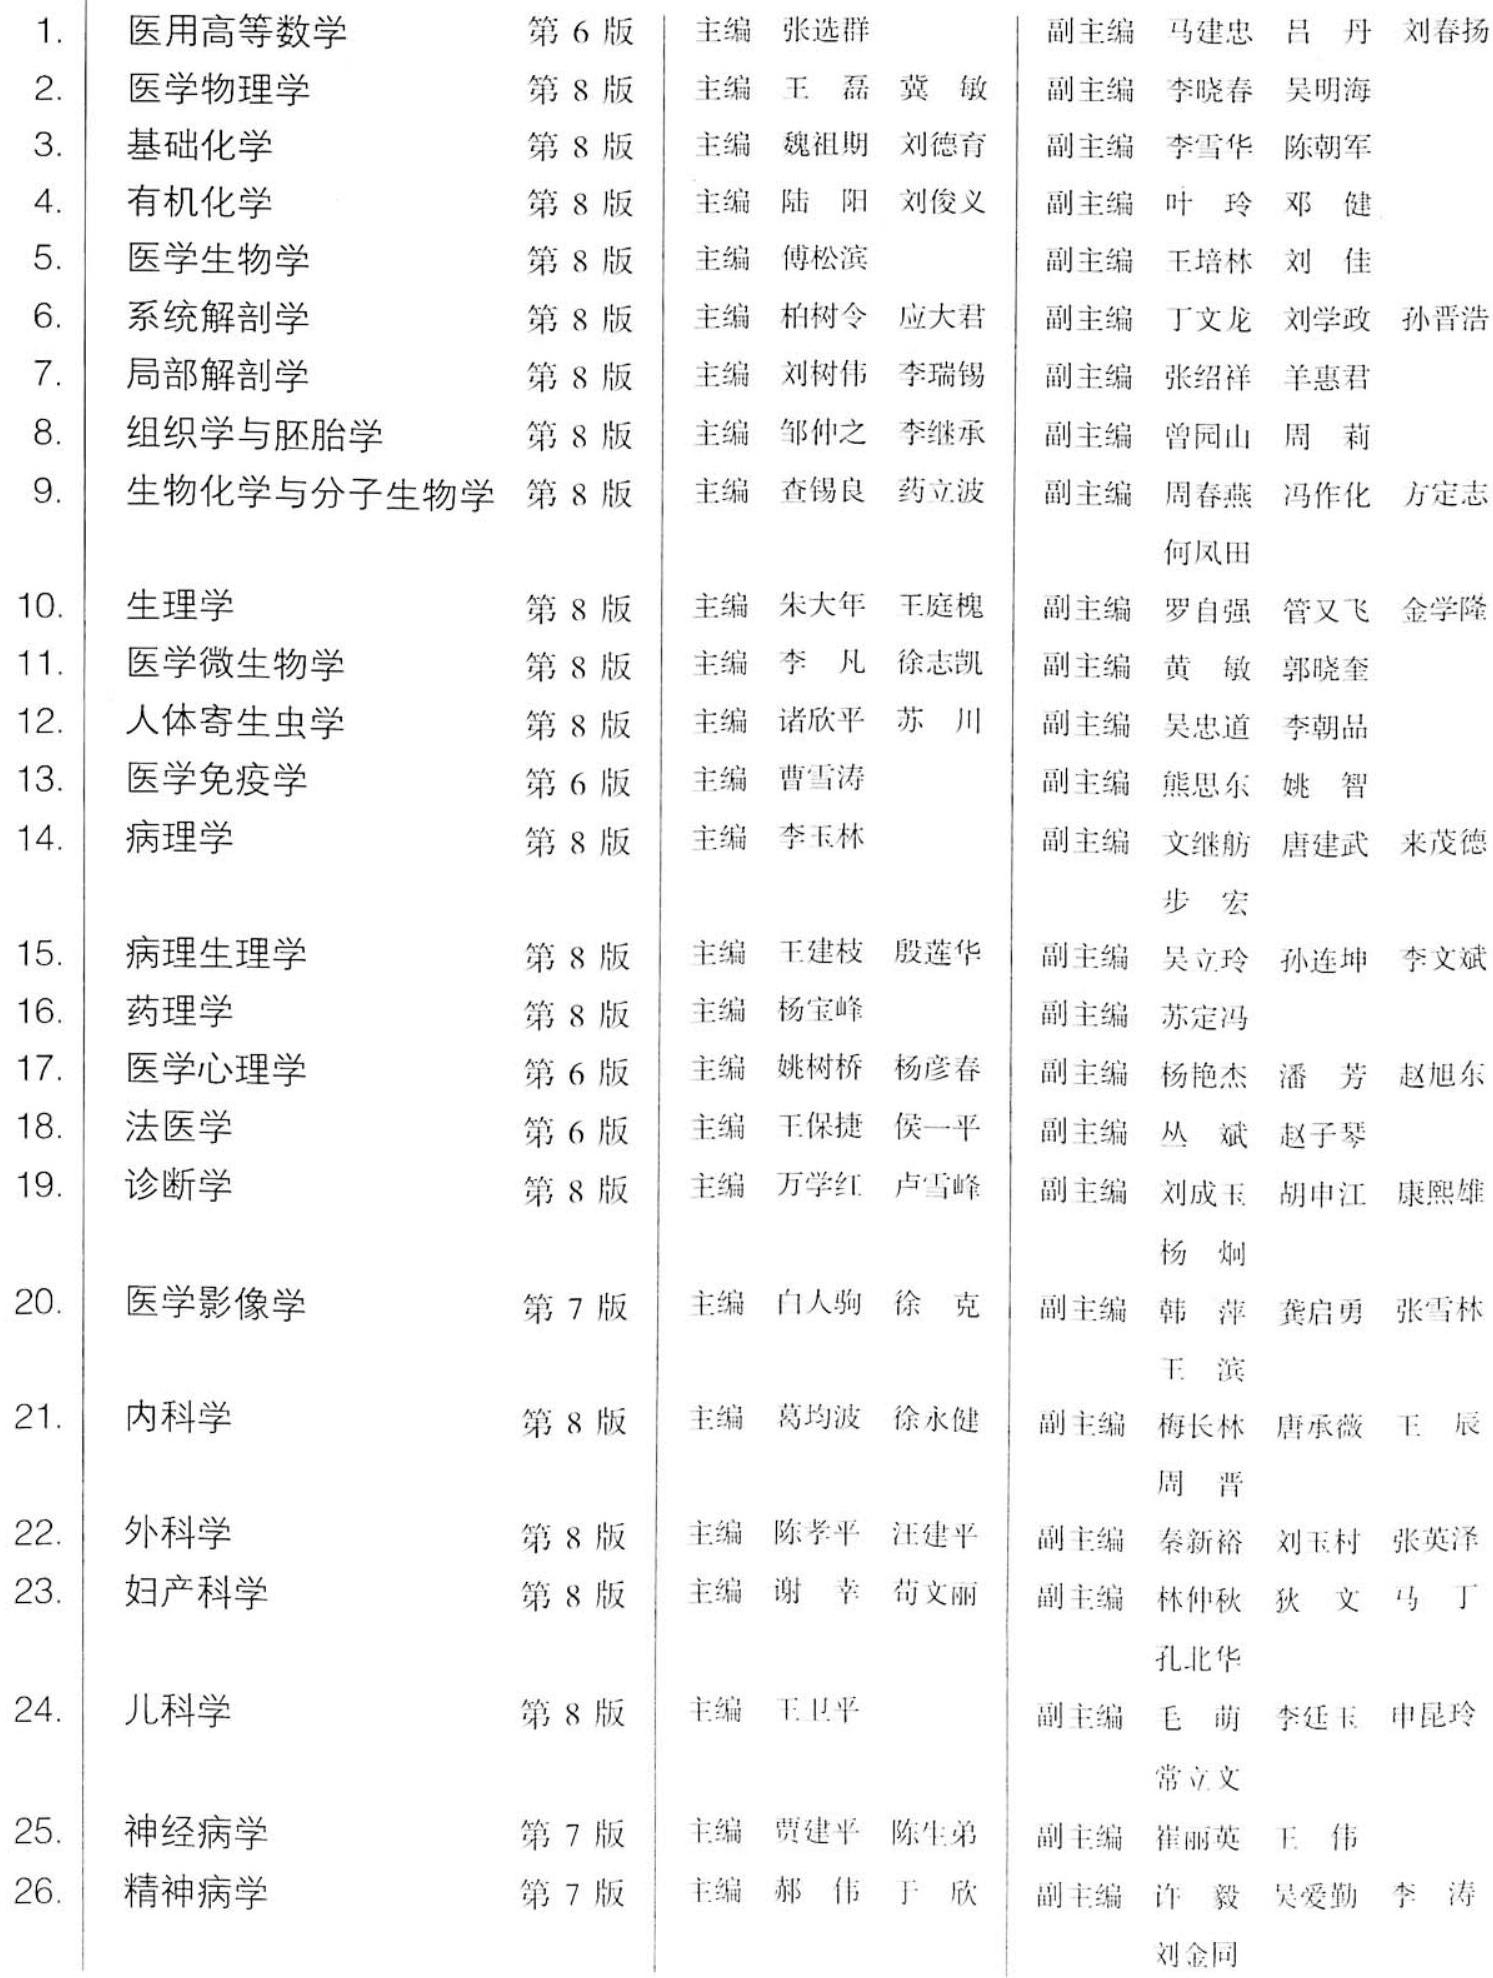
\includegraphics[max width=\textwidth]{2024_07_09_002a177993bd97d1d6d7g-006}
\end{center}

\begin{center}
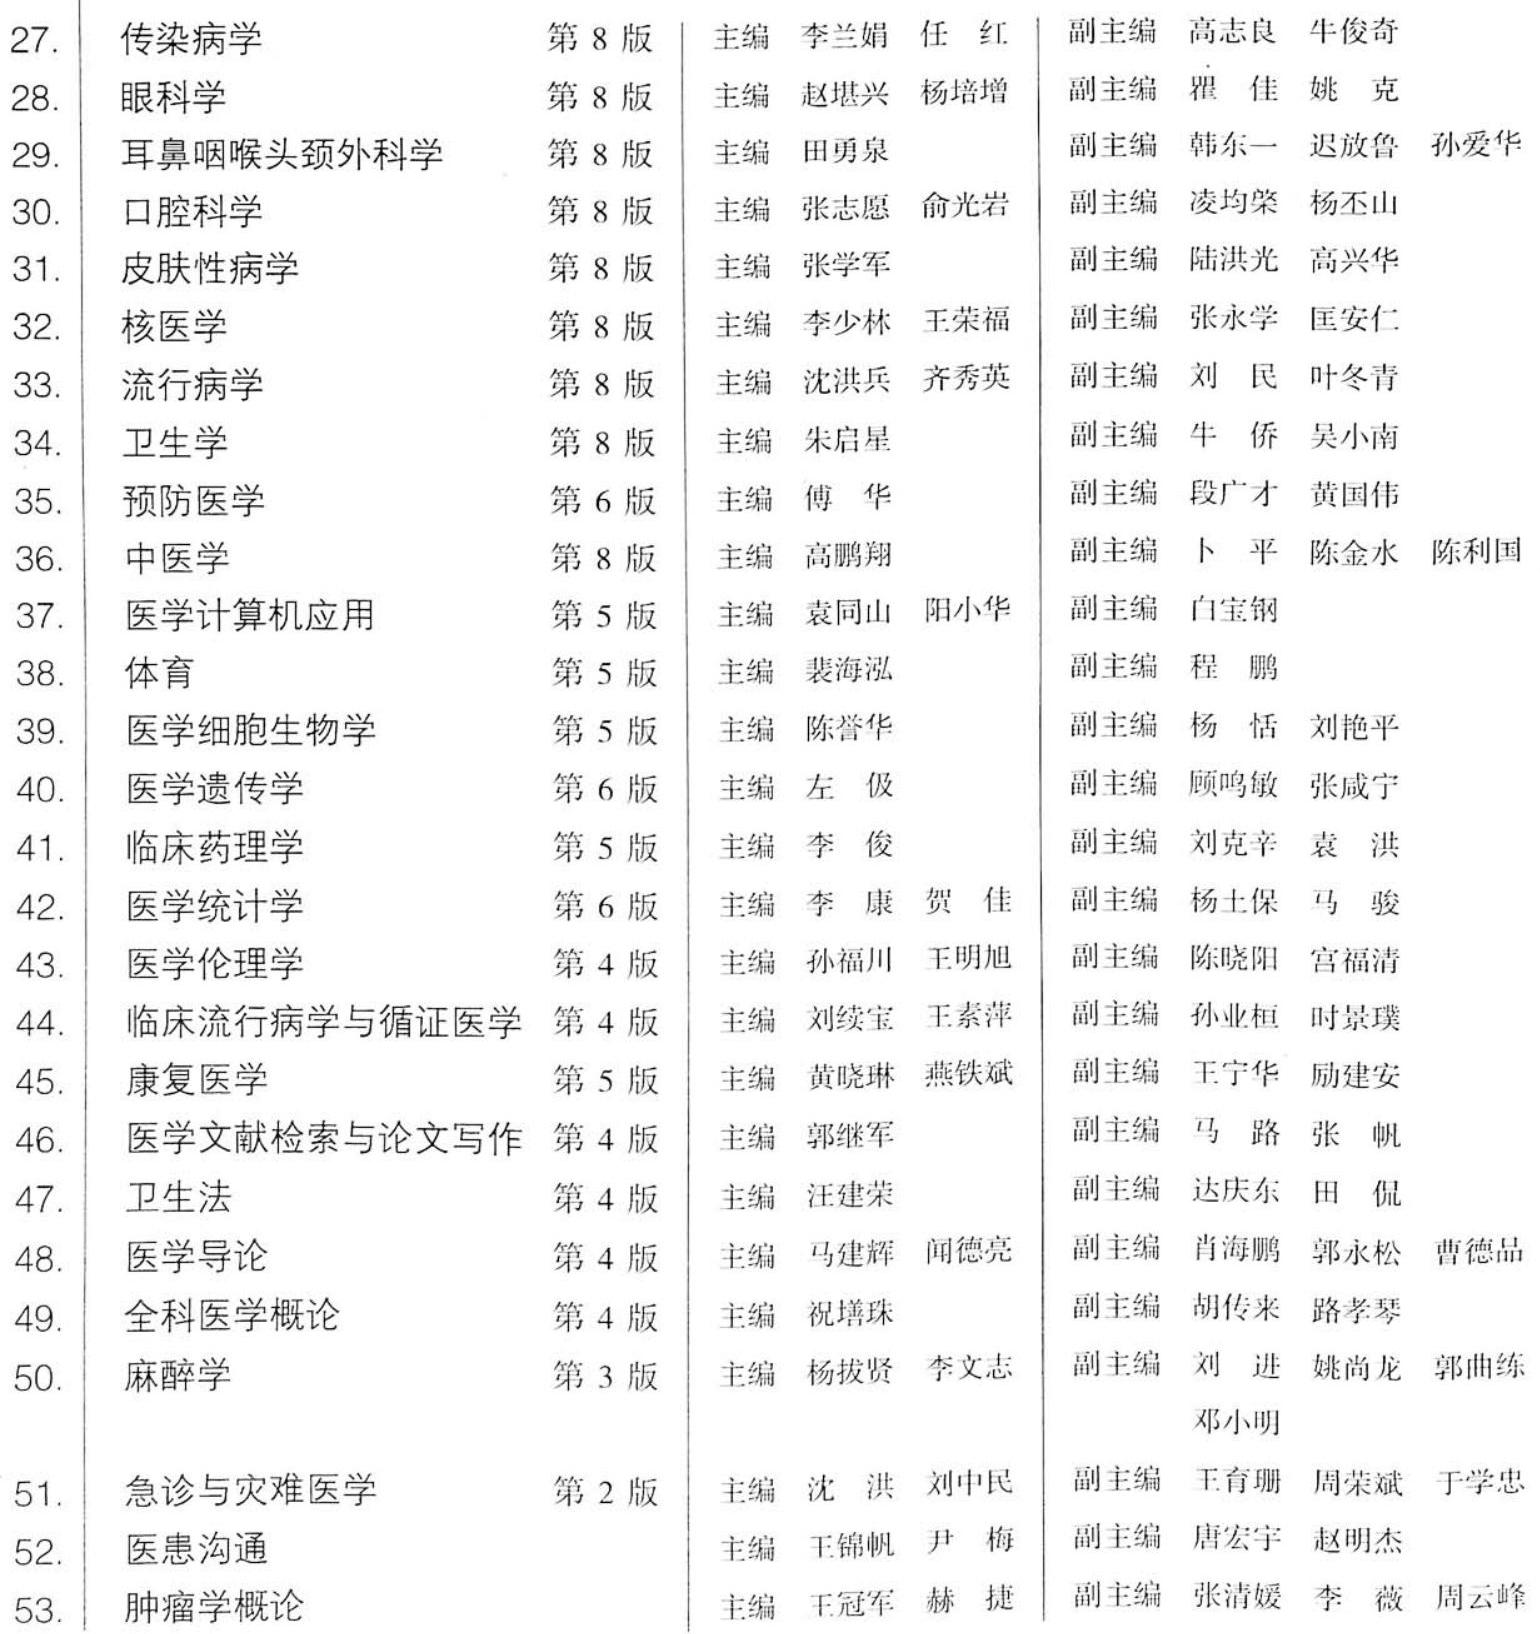
\includegraphics[max width=\textwidth]{2024_07_09_002a177993bd97d1d6d7g-007}
\end{center}

\section*{第六届全国高等学校五年制本科临床医学专业}
顾

问

沈晓明王德炳 刘德培 吴孟超刘允怡

主任委员

陈灏珠 钟南山

副主任委员

王卫平 杨宝峰 龚非力 柯 杨 石应康 郑树森

委 员(以姓氏笔画为序)

王 滨 王冠军 王家良王鸿利文历阳文民刚文继舫

孔北华 田勇泉白波向人驹冯友梅品兆丰 朱明德

刘吉成 国剑群 李玉林 步 宏 吴在德 吴肇汉 汪建平

沈悌 陆再英 郎景和 赵 群赵玉沛南登峕柏树令

曹雪涛 崔慧先 葛均波 曾因明 曾哓荣 雷 寒 䍜 佳

\begin{center}
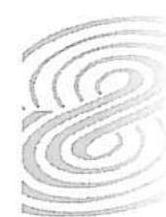
\includegraphics[max width=\textwidth]{2024_07_09_002a177993bd97d1d6d7g-009}
\end{center}

高水平、高质量的医学教育既是办好人民满意教育的重要组成部分,也是医疗卫生事业改革发展的重要支撑。随着我国医药卫生体制改革的不断深人,对高等医学教育改革也提出了更高的要求。如何培养适应国家需要、人民满意的高质量、高水平医学人才是当前医学教育的首要任务。为此,在 “十二五”开局之年,教育部和卫生部共同组织实施了医学教育综合改革。

医学教育综合改革要求我们深人贯彻落实教育规划纲要和医药卫生体制改革的意见,整循医学教育规律, 以改革创新为动力, 着力于医学教育发展与医药卫生事业发展的紧密结合, 着力于人才培养模式和体制、机制的重点突破,着力于医学生职业道德和临床实践能力的显著提升,着力于医学教育质量保障体系的明显加强, 从而全面提高医学人才培养质量,为发展医药卫生事业和提高人民健康水平提供坚实的人才保障。

教材建设在提高人才培养质量中发挥着重要的基础性作用, 对此教育部一直高度重视, 要求以教材建设为抓手,推动医学课程和教学方法改革。一本好的教材,给医学生以正确的引导,给临床医生以正确的指导。人民卫生出版社作为国家级优秀出版单位,承担了大量教材的规划和出版工作,形成了课程种类齐全、学科体系合理、配套服务全面的教材出版模式。尤其是在以吴阶平、裴法祖、吴孟超、陈䫏珠等院士为代表的老一辈医学大家的付出和带领下, 在一大批医学教育精英的努力和参与下,其出版的五年制本科临床医学专业规划教材为我国矢学界培养了一代又一代优秀的医药学人才,为推动我国医疗卫生事业的改革和发展做出了巨大的历史贡献。

此次第八轮五年制本科临床医学专业规划教材的修订工作是在贯彻觉的十八大关于“深化教育领域综合改革” 精神的背景下,在落实卫生部、教育部联合下发的《关于实施临床医学教育综合改革的若干意见》的基础上启动的。修订工作贯穿了医学教育综合改革的要求,特别是注重将医德教育贯穿于医学教育的全过程,增加了《医患沟通》一书,同时强化临床实践教学, 配套编写了相关的实践指导,以提高医学生的临床实践能力。

我们相信, 在教育、卫生系统的通力合作下, 在广大医学教育工作者的大力支持利参与下,第八轮五年制本科临床医学专业规划教材的修订出版对推动矣学教育综合改革,提高矣学人才培养质量将产生积极的推动作用

教育部部长助理

\begin{center}

\includegraphics[max width=\textwidth]{2024_07_09_002a177993bd97d1d6d7g-009(1)}
\end{center}

2013年 3 月

\begin{center}
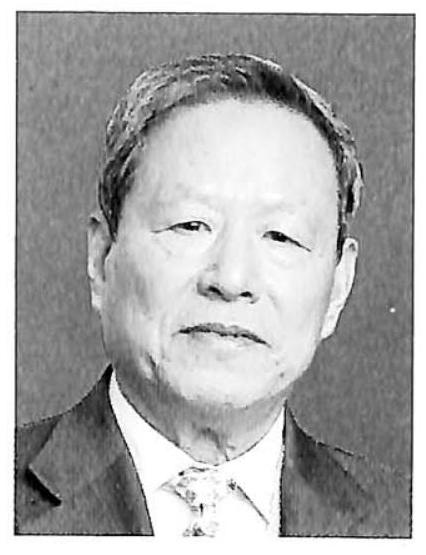
\includegraphics[max width=\textwidth]{2024_07_09_002a177993bd97d1d6d7g-010}
\end{center}

\section*{曾因明}
男, 主任医师, 教授, 榑士研究生导师, 1935 年 11 月出生于江苏江阴县。现任徐州医学院终身教授、麻醉学院名誉院长、江苏省麻醉医学研究所所长。兼任《国际麻醉学与复苏杂志》总编、全国高等医学教育学会麻醉学教育研究会理事长, 江苏省麻醉科医疗质量控制中心主任。享受国务院政府特殊津贴。

1959 年毕业于北京医学院, 从事麻醉学专业五十余年。先后获得:国家教委、人事部授予的全国优秀教师称号; 江苏省政府授子的突出贡献中青年专家, 优秀研究生导师称号; 省教委授了的优秀学科带头人, 省教委红杉树园丁奖金奖;获得江苏省优秀医学重点学科带头人称号与重奖;中国医师协会麻醉学医师分会授予的“终身成就奖”和中华医学会麻醉学分会授予的“突出贡献奖”。承担全国自然科学基金 2 项, 部、省级课题 4 项; 发表论文 108 篇, 其中 20 余篇论文被 SCI 收录; 获国家、省、部级成果奖、科技创新奖 16 项; 获重大发明专利两项。出版专著教材 26 部, 主译 Miller's Anesthesia, 参与主编《现代麻醉学》和《麻醉学新进展》。在担任麻醉学教材编审委员会主任期间, 主持完成“麻醉学专业(本科)教材”一套七部(第3 版); “住院医师培训教材”一套四部; “麻醉学 (临床医学专业用) 教材”(第2版)。

. .\\
.

\begin{center}
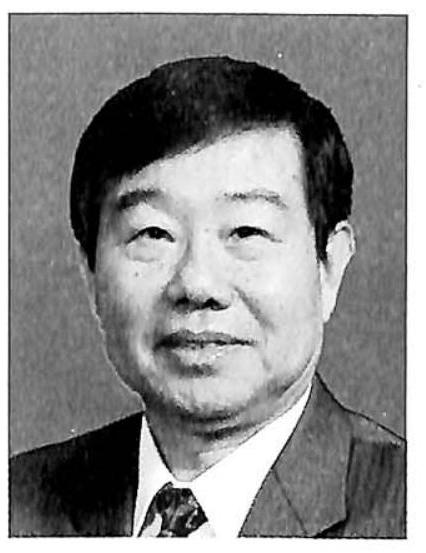
\includegraphics[max width=\textwidth]{2024_07_09_002a177993bd97d1d6d7g-012(1)}
\end{center}

\section*{杨拔贤}
男, 主任医师, 教授, 博士研究生导师。1946 年 4 月出生于江西省鄱阳县。现任北京大学医学部麻醉学系主任、学位与研究生教育委员会委员、医疗质量管理委员会委员, 人民医院学术委员会委员; 卫生部专业技术资格考试委员会麻醉学专家委员会副主任委员; 中华医学会、北京医学会和军队总后勤部医学会医疗事故技术鉴定专家库成员。历任北京大学第一医院麻醉科副主任、人民医院麻醉科主任; 中华医学会麻醉学分会第五、六、七届常务委员,北京医学会麻醉专业委员会副主任委员。

1970 年毕业于北京医学院医疗系, 毕业后在北京大学第一医院和人民医院麻醉科工作, 从事麻醉学医教研 40 多年。1987 年在美国哈佛大学医学院麻省总医院学习。1984 年在谢荣教授领导下在我国率先建立了由麻醉科管理的 SICU。参加制定卫生部《临床住院医师规范化培训大纲》(第 1 版, 1995)。主持 2007 年国家级精品课程《麻醉和重症医学》。培养硕士研究生 16 名, 博士研究生 30 名。参加了各种教材和专著的编写, 包括《麻醉学》(第 3 版), 《外科学》(第 $4 \sim 8$ 版) 和《黄家驱外科学》(第 $6 \sim 8$ 版)。发表论文 90 余篇; 主编或副主编书籍 5 部, 参编书籍 40 多部。

\begin{center}
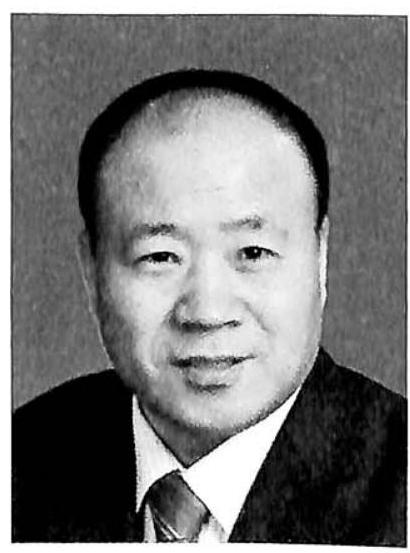
\includegraphics[max width=\textwidth]{2024_07_09_002a177993bd97d1d6d7g-012}
\end{center}

\section*{李文志}
男, 主任医师, 教授,博士研究生导师。1960 年 11 月生于黑龙江省拜泉县。现任哈尔滨医科大学麻醉学系主任、附属第二医院副院长、麻醉教研空主任、麻醉科主任; 黑龙江省麻蟀科质量控制中心主任。民盟黑龙江省委副主委, 第十届、十一届及十二届全国政协委员。黑龙江省 “龙江学者”特聘教授。黑龙江省医学会副会长, 中国医师协会麻醉学医师分会副会长, 中华医学会麻醉学分会常务委员, 黑龙江省医学会麻醉学分会主任委员, 全国高等医学教育学会麻醉学教育研究会副理事长。

从事麻醉学医教研工作 29 年。获得黑龙江省教学名师、省优秀教师、省研究生优秀指导教师等称号。主持的麻醉专业课程《危重病医学》获得国家级精品课程, 哈尔滨医科大学麻醉学专业为国家级特色专业、黑龙江省重点专业。发表论文 204 篇,SCI 收录 30 篇, 获得中华医学会麻醉学分会年度优秀SCI 论文一等奖、二等奖各 1 项。出版著作 20 部, 主持承担国家自然科学基金面上项目 4 项,教育部归国人员基金 1 项,教育部博士点基金 1 项,黑龙江省杰出青年基金 1 项、黑龙江省自然科学基金重点课题 1 项, 黑龙江省攻关重大课题 1 项。获得教育部科技进步二等奖 1 项、黑龙江省政府科技进步二等奖 2 项。

.

.

,

\begin{center}
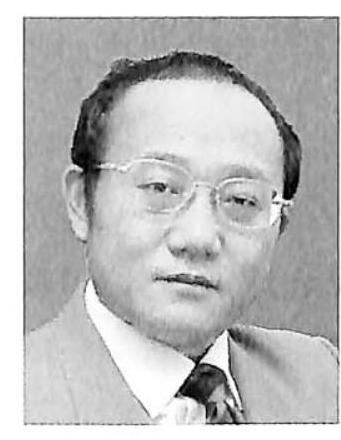
\includegraphics[max width=\textwidth]{2024_07_09_002a177993bd97d1d6d7g-014}
\end{center}

\section*{刘 进}
男, 主任医师,教授,博士研究生导师。1956 年 8 月生于湖北省恩施市。现任中华医学会麻醉学分会主任委员, 四川大学华西医院麻醉与重症医学教研室主任和转化神经科学中心主任。历任中国医师协会麻醉学医师分会首任会长。

从事麻醉学医教研工作 25 年。主要从事吸人麻醉和血液保护的临床和研究工作。国家自然科学基金杰出青年基金获得者和教育部“长江学者奖励计划”特聘教授。发表 SCI 论文 120 余篇。“吸人麻醉的研究”获国家科技进步二等奖, “围手术期血液保护”获四川省科技进步一等奖。

\begin{center}
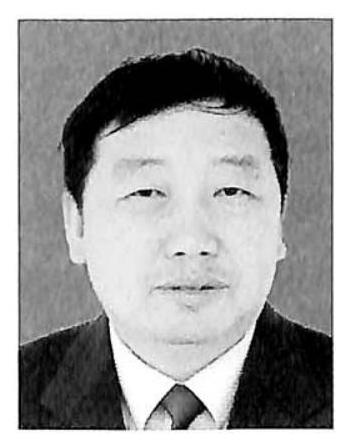
\includegraphics[max width=\textwidth]{2024_07_09_002a177993bd97d1d6d7g-014(2)}
\end{center}

\section*{姚尚龙}
男, 主任医师, 教授,博士研究生导师。1956 年 3 月生于安徽䒴湖。卫生部有突出贡献中青年专家, 享受国务院特殊津贴。现任华中科技大学同济医学院附属协和医院副院长兼麻醉与危重病学教研室主任; 中华医学会麻醉学分会副主任委员; 中国医师协会麻醉学医师分会会长; 世界疼痛医师学会中国分会副主任委员; 世界卫生组织中国初级创伤救治培训副主席等。

从事麻醉学医教研工作 30 余年。先后主持 5 项国家自然基金,获湖北省科技进步一、二等奖, 中华医学会科技进步三等奖, 卫生部优秀教材二等奖等。发表论文 300 余篇, 主编和参编专著 30 余部。

\begin{center}
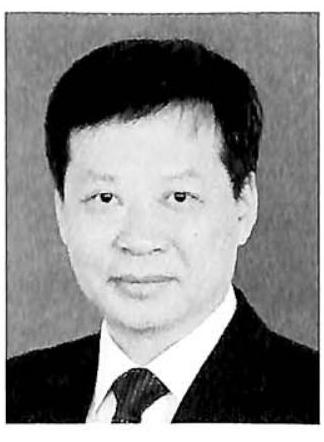
\includegraphics[max width=\textwidth]{2024_07_09_002a177993bd97d1d6d7g-014(1)}
\end{center}

\section*{郭曲练}
男,主任医师,教授,博士研究生导师。1958 年 10 月出生于北京市。现任中南大学湘雅麻醉学系主任、湘雅医院麻醉与重症医学教研室主任; 中华医学会麻醉学分会常委, 湖南省麻醉学会主任委员。

从事麻醇学医教研工作 30 余年。获国家自然科学基金等 5 项、省部级课题 10 余项; 获湖南省科技二等奖 2 项、三等奖 1 项, 获国家专利 4 项。主持国家精品课程《临床麻醉学》和国家临床重点专科项目。主编教村《临床麻醉学》(第 3 版) ; 2007 年获中南大学第三届教学名师。发表论文 200 余篇, 其中 SCI 收录论文 30 余篇。培养博,硕士研究生 80 余人。

\begin{center}
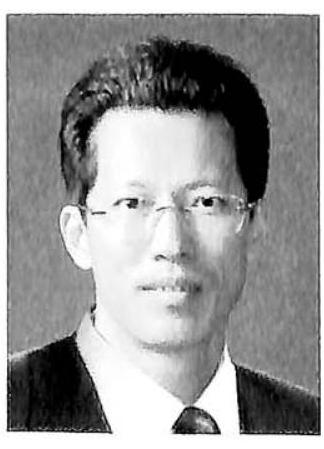
\includegraphics[max width=\textwidth]{2024_07_09_002a177993bd97d1d6d7g-014(3)}
\end{center}

\section*{邓小明}
男, 主任医师, 教授, 博士研究生导师。1963 年 1 月出生于江西吉安。现任第二军医大学附属长海医院麻醉科、麻醰学教研室主任; 中国高等教育学会医学教育专业委员会麻醉学教育研究会副理事长等; 全军麻醉学与复苏专业委员会副主任委员,中华医学会麻醉学分会常务委员,上海市麻醉学专科委员会候任主任委员。

从事麻醉学医教仾工作 29 年, 获国家自然科学基金多项, 获军队医打成果二等奖两项。主编或主译书籍 16 部, 发表 SCI 论文 30 余篇。获得总后勤部“育才奖”银奖, 上海市“曙光学者”、医学领军人才利领军人才等称号。培养博上生 30 名、硕士生: 38 名。

\begin{center}
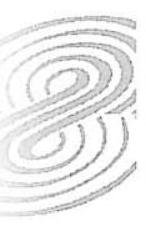
\includegraphics[max width=\textwidth]{2024_07_09_002a177993bd97d1d6d7g-016}
\end{center}

“麻醉学”是临床医学的一个重要学科, 是随着临床医学 (尤其是外科学) 、基础医学和医学生物工程等现代科学的发展而逐渐形成的,同时也促进了临床学科的进步和发展。手术疼痛曾是妨碍外科发展的重要因素之一,1846 年 Morton 在美国麻省总医院 (MGH) 公开演示乙醚麻醉获得成功, 为外科学的发展奠定了基础。然而, 手术对机体的影响不仅是疼痛, 还能引起各种生理功能的变化;麻醉虽然能解决手术疼痛的问题,但也可影响生理功能,甚至可危及生命, 手术无痛是以生理代价而获得的。因此, 在手术麻醉期间如何维持和调控患者的生理功能, 不仅是麻醉学的重要内容,而且其难度和所需知识的深度及广度都比单纯消除手术疼痛更为困难和复杂。在围术期,麻醉科医师使用各种监测技术最为频繁,对呼吸道的控制和呼吸管理最为熟悉,术中大量、快速输液输血, 使用各种血管活性药物的机会最多。因此, 在临床实践中逐渐形成的麻醉学理论和技术,包括病情评估、气道管理、器官功能监测、心肺复苏和疼痛治疗等, 已经广泛地应用于手术室以外的诊疗工作中, 并派生出重症医学科和疼痛诊疗科。对于临床医学生来说,无论将来从事何种专业,都可以应用麻醉学的基本理论和技术来分析、处理临床问题,尤其是对重症患者的监测、病情判断和处理。因此, 学好麻醉学不仅可以拓宽临床思路,而且可在临床工作中增强发现问题、分析问题和解决问题的能力。根据现今医学生知识结构的需要, 在编写本教材的过程中,我们力求从宏观层面介绍临床麻醉的方法和实施,而将麻醉学的核心理论和技术,包括围术期生命功能的监测和调控、重要脏器功能的维护和治疗、疼痛诊疗等, 从理论到实践作了较深人、易懂的介绍, 以适合现代医学教育的需要。

本教材在编写主导思想上听取了多位资深医学专家、知名麻醉学专家的意见和建议, 曾因明教授对教材编写的内容、深度以及质量控制等方面提出了系统的建议,在编写过程中得到了各位编者的理解、支持和无私的奉献。在此表示衷心的感谢。但要成为一本成熟的优秀教材仍需要不断总结、改进和完善,相信在全国麻醉界同仁的共同努力下,在传承中将使《麻醉学》越编越好。

\section*{杨拔贤李文志}
2013 年 2 月\\
第一节 概述 1

第二节 麻醉学的发展 1

第三节 麻醉科的组织结构与内涵 3

一、临床医疗工作 4

二、科研工作 6

三、教育工作 6

第四节 学好麻醉学 6

第一节 术前访视与术前病情评估门诊 7

第二节 手术前病情评估的流程和方法 8

一、手术前病情评估的流程 8

二、手术前病情评估的方法 10

第三节 麻醉前准备和用药 14

一、麻醉前准备 14

二、麻醉前用药 16

第三章 $\quad$ 局部麻醉 19

第一节 局麻药 19

一、分类和理化性质 19

二、作用机制 21

三、临床药理学 21

四、影响局麻药药理作用的因素 22

五、局麻药的毒性反应 23

第二节 局部麻醉 24

一、表面麻醉 24

二、局部浸润麻醉 24

三、区域阻滞 25

四、静脉局部麻醉 25

第三节 神经阻滞 26

一、概述 26

二、颈神经丛阻滞 26\\
第一节 椎管内解剖与麻醉生理 33

一、椎管解剖 33

二、椎管内阻滞的生理 35

第二节 蛛网膜下弥阻滞 36

一、蛛网膜下陌阻滞的临床应用 36

二、蛛网膜下祘阻滞的并发症 38

第三节 硬膜外阻滞 39

一、硬膜外阻滞的临床应用 39

二、硬膜外阻滞的并发症 42

三、骶管阻滞 44

第四节 蛛网膜下隙-硬膜外联合阻滞 44

第一节 全身麻醉药 46

一、吸入麻醉药 46

二、静脉麻醉药 49

三、肌肉松驰药 50

四、麻醉性镇痛药 52

第二节 全身麻醉的实施 52

一、全身麻醉诱导 52

二、全身麻醉维持 53

三、全身麻醉深度的判断 54

四、麻醉苏政 55

第三节 全身麻醉的并发症及其处理 56

\section*{第一节 影响气道通畅的原因 58}
一、气道的结构 58

二、影响解剖气道通畅的常见原因 59

第二节 维持气道通畅的方法 60

一、维持气道通畅的基本方法 60

二、面罩通气 62

三、气管插管术 63

四、气管切开术 67

五、喉罩通气道的应用 68

六、食管一气管联合导管的应用\\
第三节 困难气道的处理 70

一、困难气道的定义及其评估 71

二、困难气道的处理 71

一、控制性降压的生理基础

二、控制性降压对机体的影响

三、控制性降压适应证和禁忌证

四、控制性降压的实施 75

五、控制性降压的并发症及防治

一、体温的生理调节

二、麻醉手术期影响体温的因素

三、围术期体温异常对患者的影响

79

四、围术期体温保护

80

五、低温麻醉

80

第一节 概述 83

第二节 工作常规和离室标准 83

一、工作常规 83

二、离室标准 83

第三节 PACU 常见并发症 84

一、呼吸系统并发症 84

二、循环系统并发症 85

三、术后恶心呕吐 85

四、躁动与寒战 86

五、神经系统并发症 86

六、低体温 86

七、肾脏并发症 86

一、概述

二、ICU 的主要任务与工作职责 87

三、ICU 的收治对象和转出标准 88

四、ICU 监测项目 88

五、ICU 治疗 90

\begin{verbatim}
第一节 呼吸功能的一般监测 91
第二节 通气功能的监测 91
第三节 氧合功能的监测 93
第四节 小气道功能的监测 97
第五节 呼吸力学监测 98
\end{verbatim}

第十二章 急性呼吸衰竭 102

第一节 概述 102

一、概念 102

二、ALJ/ARDS 的病因 102

第二节 病理生理及发病机制 103

一、病理变化 103

二、病理生理改变 103

三、发病机制 104

第三节 临床表现 105

一、症状和体征 105

二、影像学所见 105

三、实验室检查 106

四、ALJ/ARDS 的分期 106

第四节 诊断与治疗 107

一、诊断 107

二、鉴别诊断 108

三、治疗 109

第十三章

呼吸治疗

113\\
第一节 氧治疗 ..... 113\\
第二节 胸部物理疗法 ..... 115\\
第三节 机械通气治疗 ..... 117\\
一、适应证 ..... 118\\
二、机械通气模式 ..... 119\\
三, PEEP ..... 120\\
四、机械通气的并发症 ..... 121\\
五、机械通气的撴离 ..... 122\\
第十四章

体外循环和体外膜肺氧合

124\\
第一节 体外循环 ..... 124\\
一、基本概念和原理 ..... 124\\
第一节 围术期水、电解质平衡的监测

143

一、体液中的水、电解质成分 143

二、水、电解质平衡的调节

143

三、常见水、电解质平衡失常的诊断与处理

第二节 围术期体液渗透浓度平衡的监测 146

一、体液渗透的基本概念 146

二、体液渗透浓度的监测方法 147

三、常见体液渗透平衡失常的诊断与处理 147

第三节 围术期酸碱平衡的监测 149

一、酸碱平衡的基本生理 149

二、酸碱平衡的监测 149

三、常见酸碱平衡失常的诊断与处理 150

第十七章

围术期的液体治疗

第一节 围术期有效循环血容量的评估 153

一、体液量的分析 153

二、无创循环监测指标 154

\begin{center}
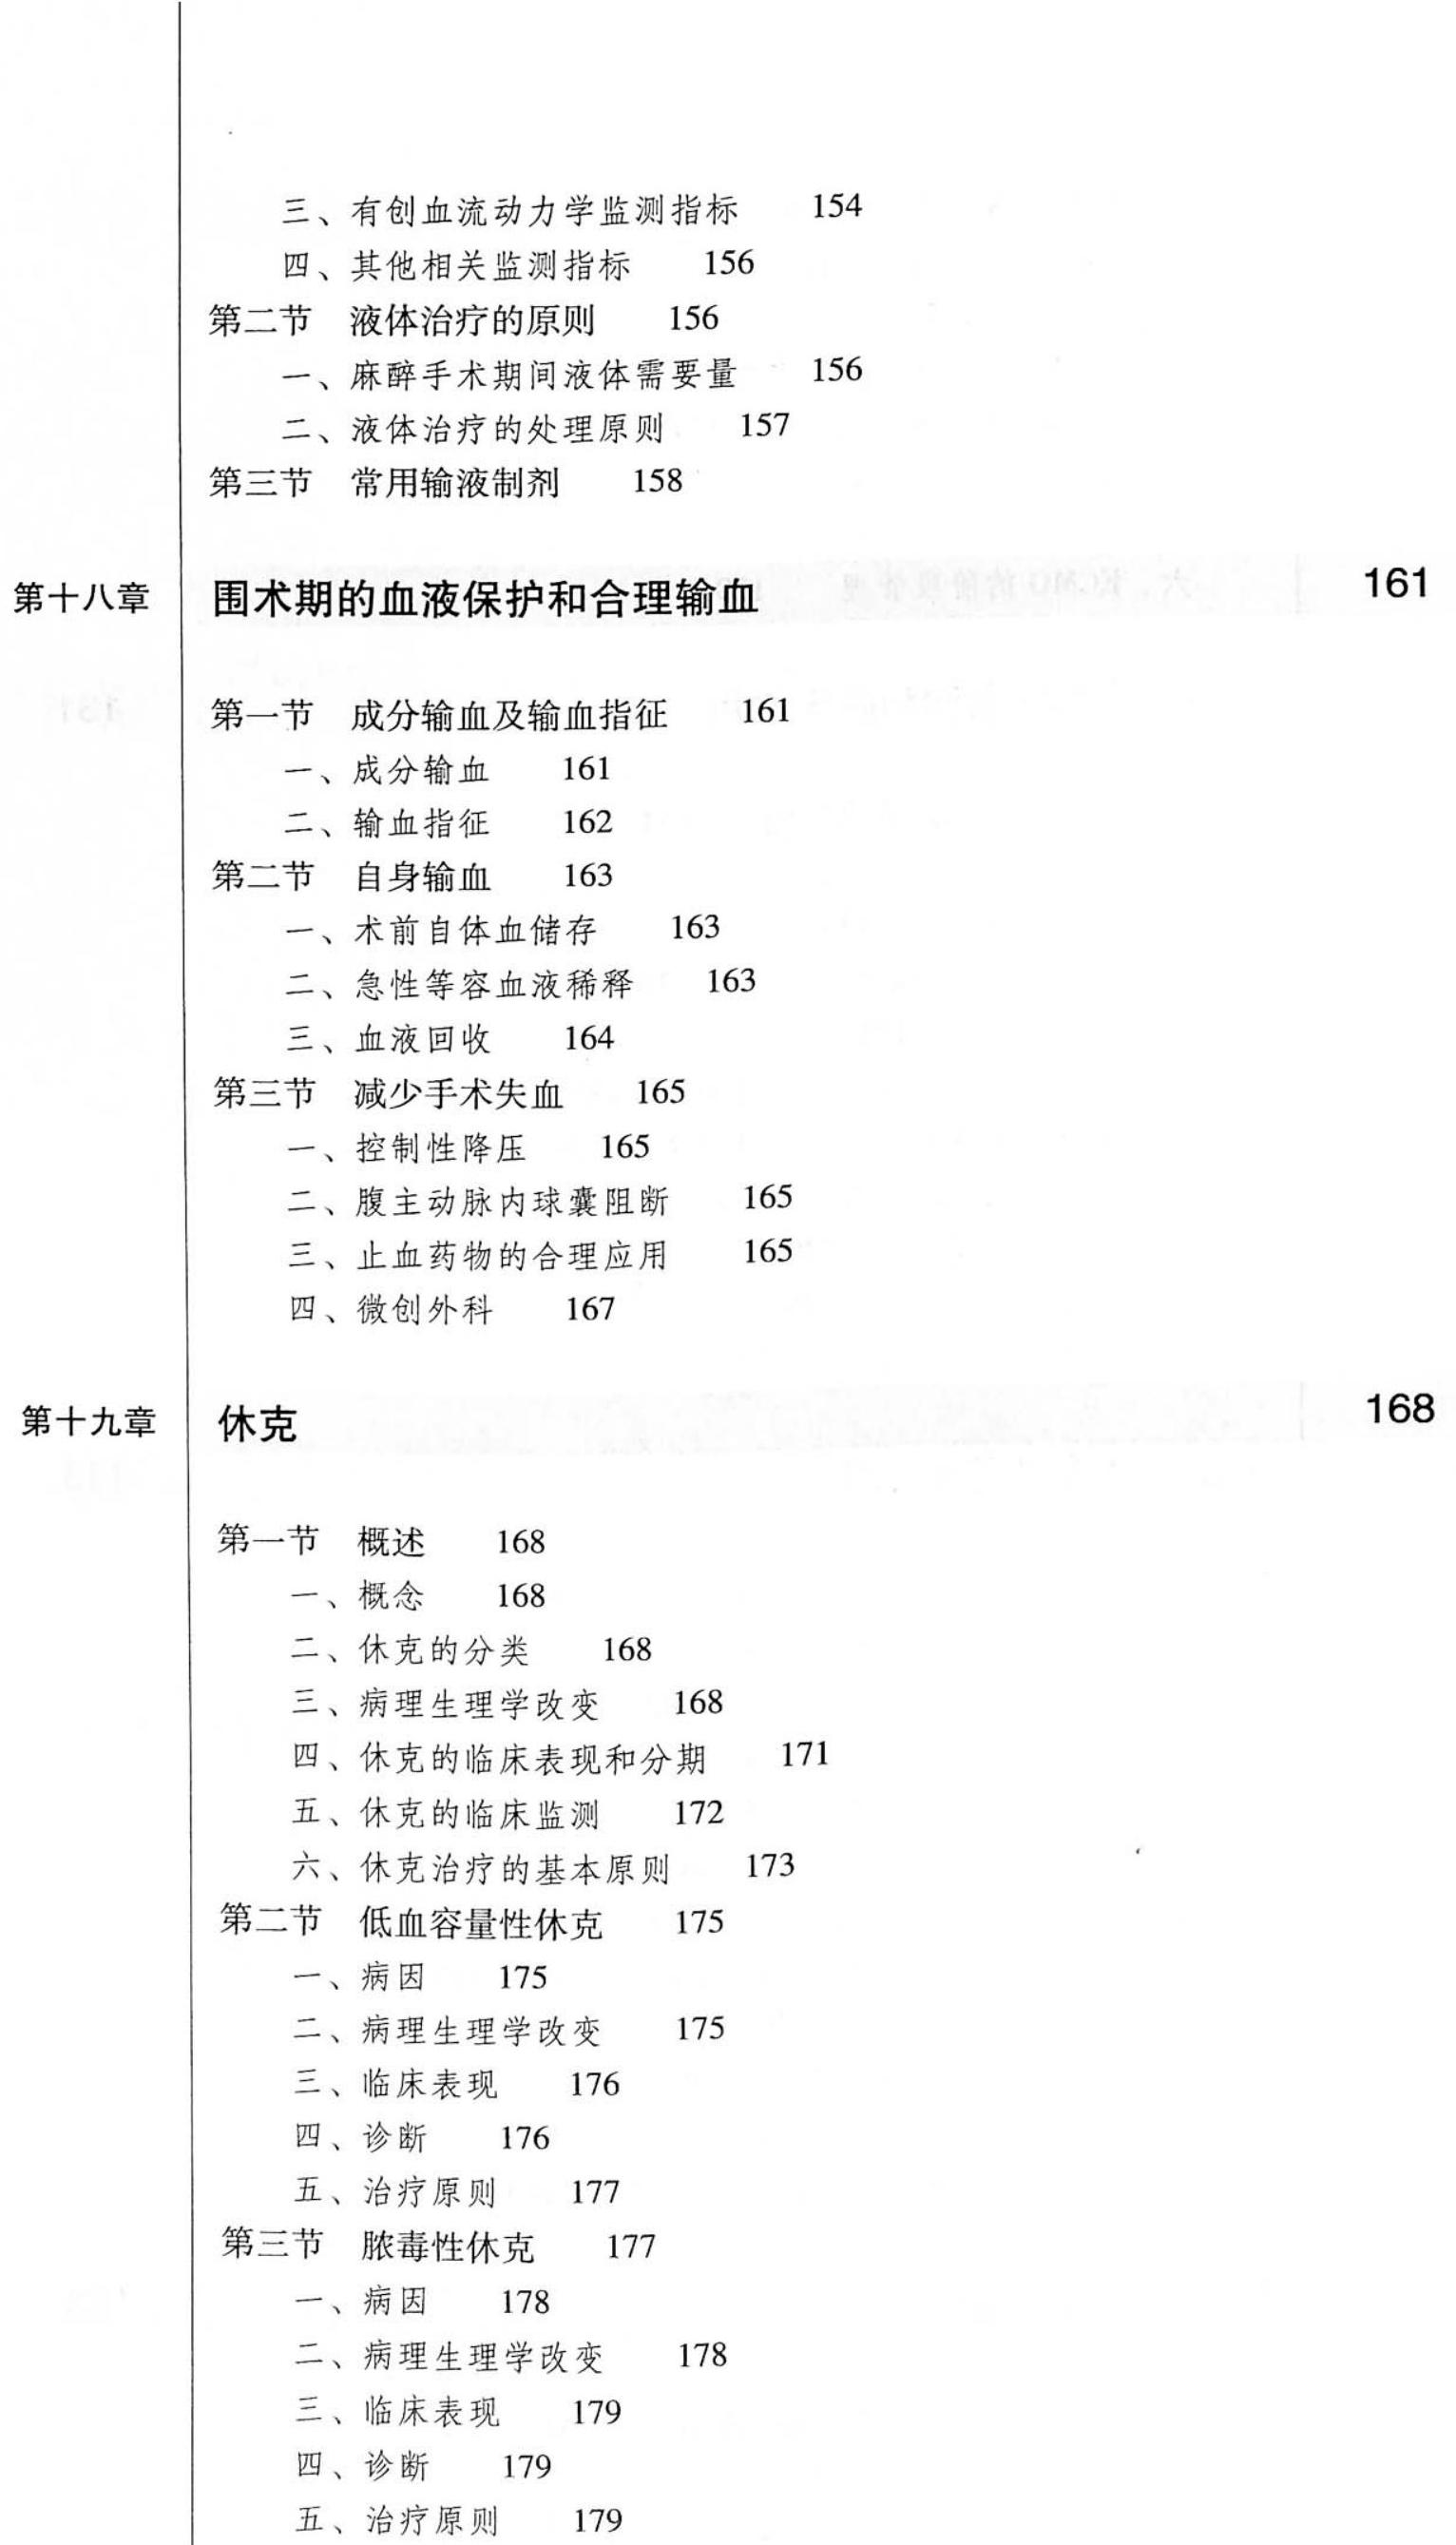
\includegraphics[max width=\textwidth]{2024_07_09_002a177993bd97d1d6d7g-023}
\end{center}

\section*{镇静的临床应用}
第一节 镇静对生理的作用 193

第二节 常用镇静药和拮抗药 194

第三节 镇静的临床应用 196

一、镇静的适应证 196

二、镇静的目标 196

三、镇静期间的监测 196

四、镇静的撒离标准 197

五、常用镇静技术 198

六、镇静的并发症及处理 199

第一节 病因和分型 201

一、病因 201

二、发病过程与分型 202

第二节 发病机制 203

一、缺血-再灌注损伤与 MODS 203

二、全身炎性反应综合征与 MODS 204

三、肠道动力学说 205

第三节 临床诊断、病情评估及监测 206

一、临床诊断及其分期 206

二、MODS 的临床病情评估 208

三、临床监测和检查 209

第四节 MODS 的防治原则 210

一、MODS 的预防 210

二、治疗 211

第一节 基本营养素 214

\begin{center}
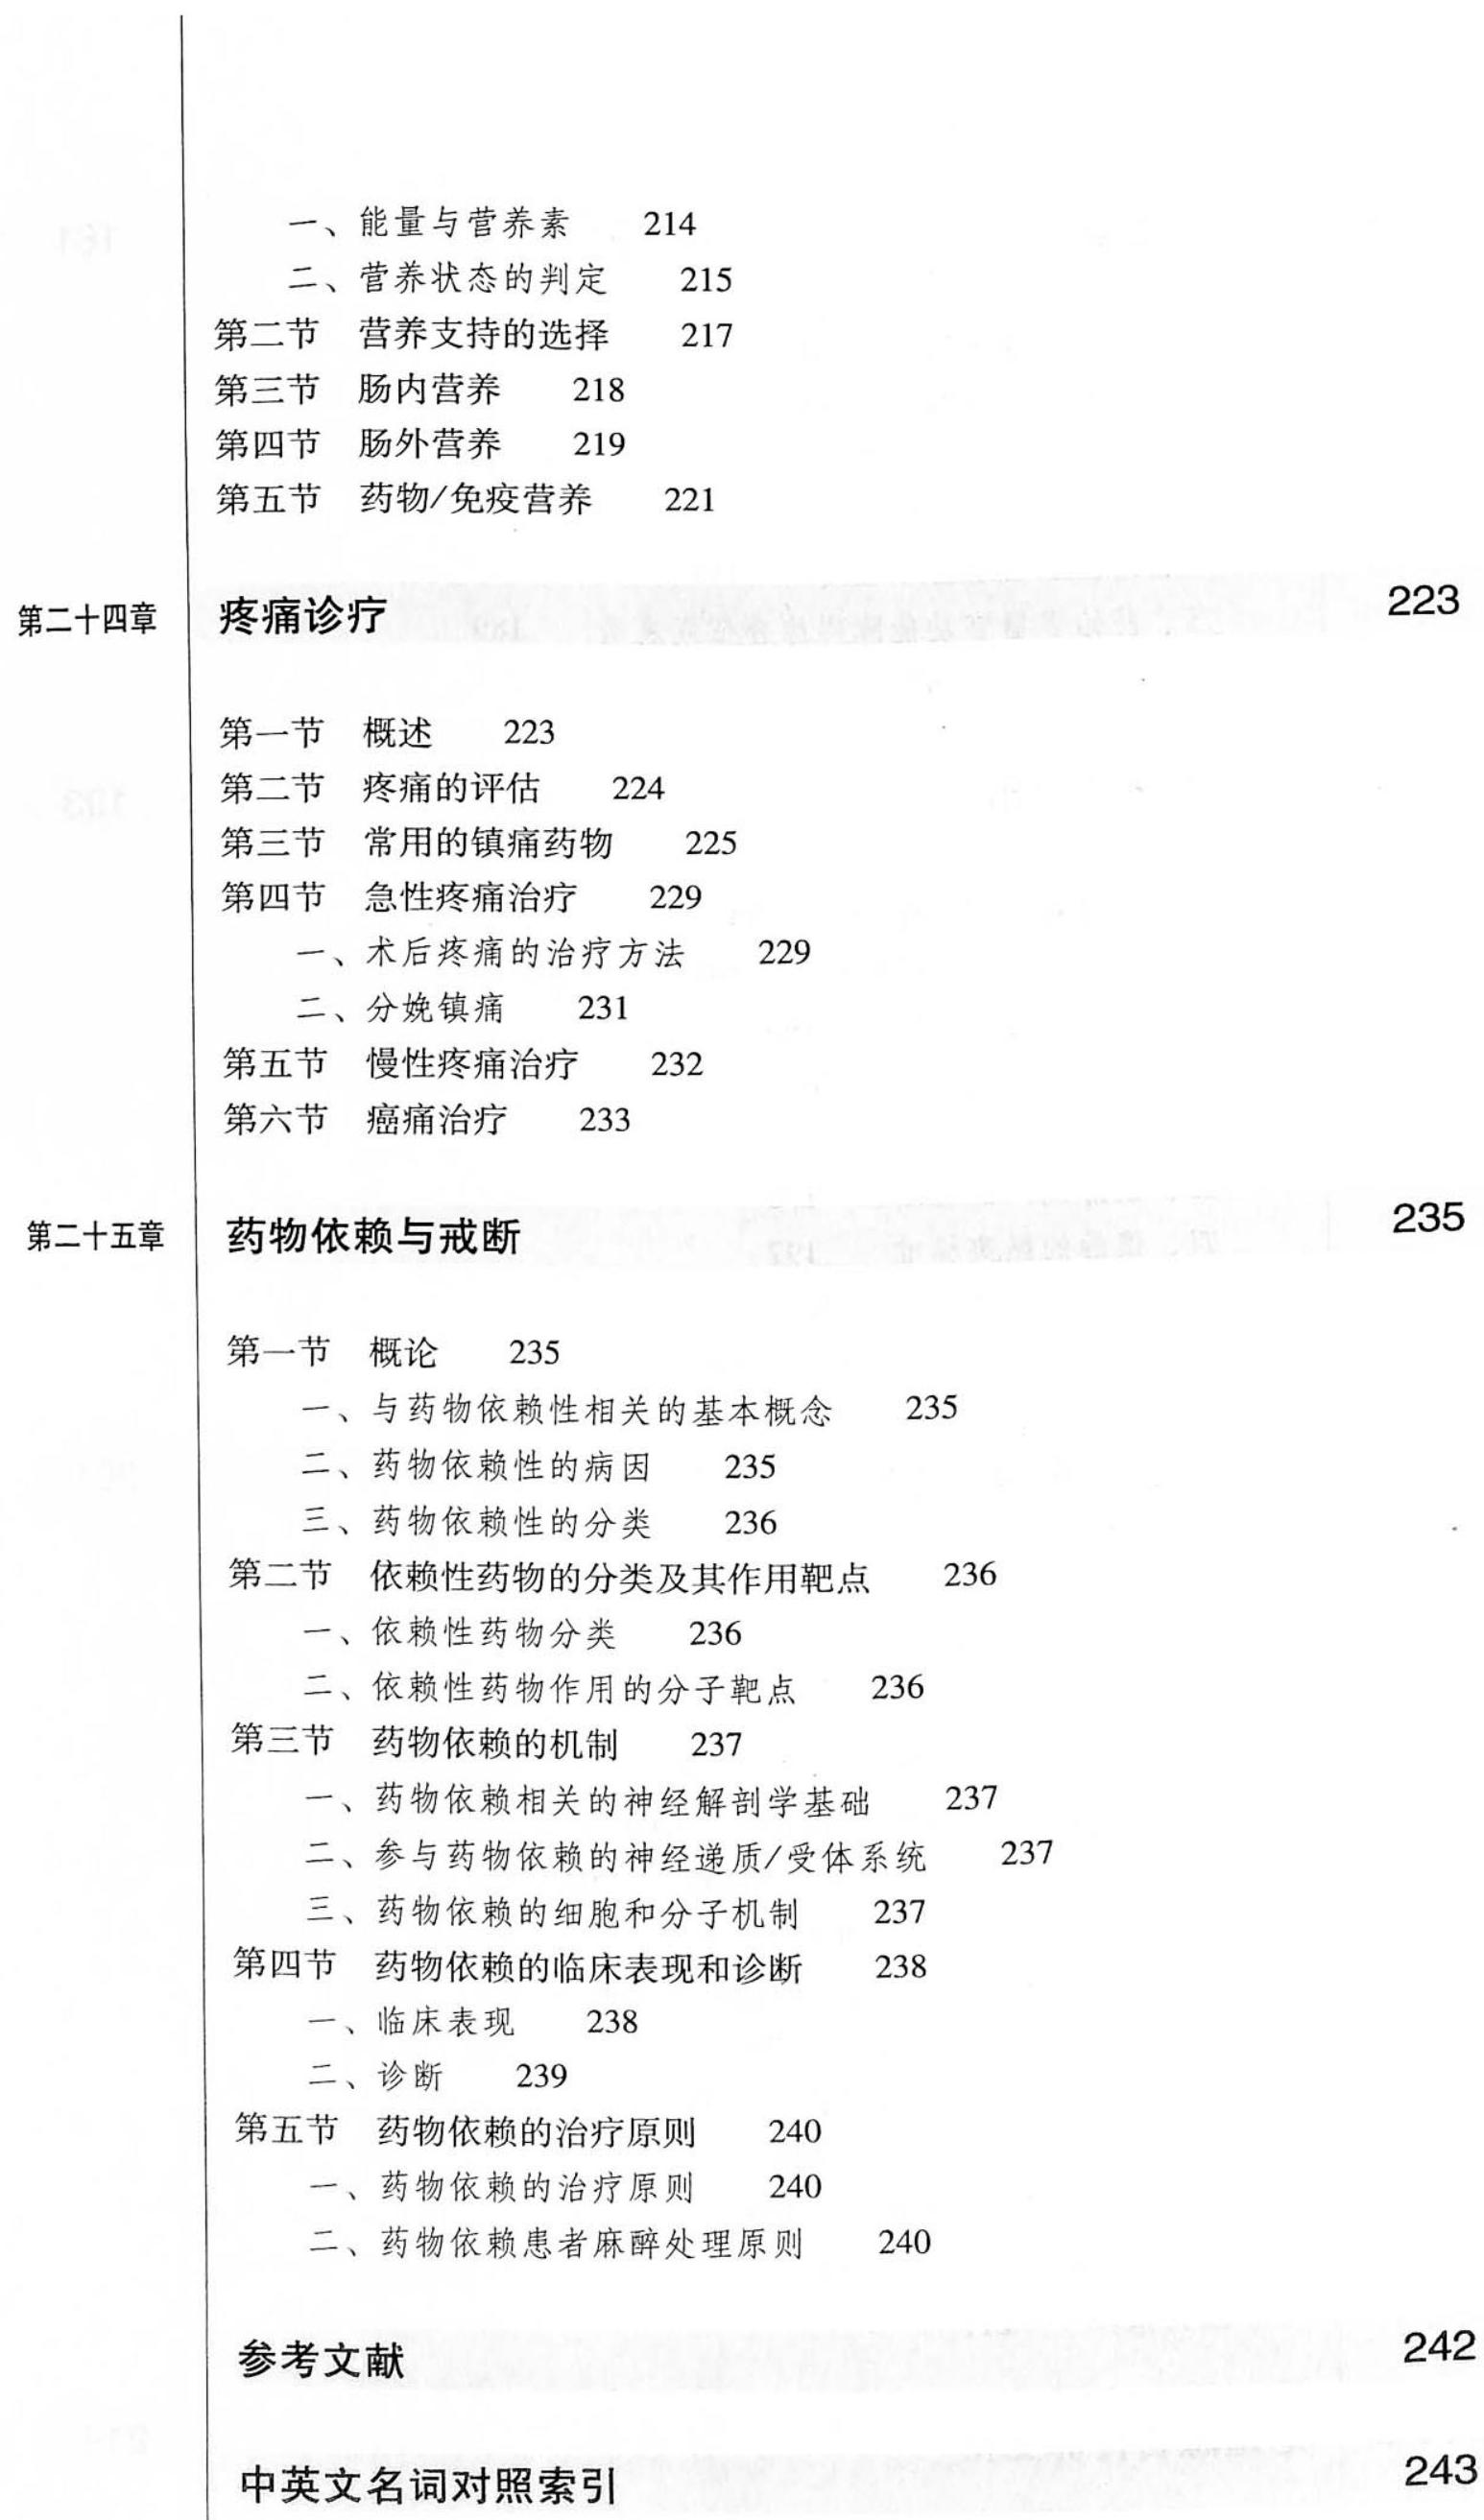
\includegraphics[max width=\textwidth]{2024_07_09_002a177993bd97d1d6d7g-025}
\end{center}

\section*{第一章 绪 论}
\section*{第一节 概 述}
19 世纪 40 年代, 乙醚麻醉成功应用于手术患者, 揭开了近代麻醉学的序幕, 迄今已有 170 多年历史。由于社会和医学科学发展的推动, 以及学科间的互相交叉、渗透与支撑, 麻醉科医师追求的目标与内涵也与时俱进。因此, 现今麻醉科医师的任务不仅是为手术顺利进行提供镇静、无痛、肌松及合理控制应激等必需条件, 更要对围术期患者生命功能进行监测、调节与控制,维护重要脏器功能, 确保患者在术后顺利康复。麻醉科的工作已从手术室内拓展到手术室外,包括门诊和病房; 其时间跨度也延伸到围术期,除术中外, 还包括术前和术后; 其内涵包括一切与患者安全、生存质量有关的领域; 不仅有专业技术, 更有系统的专业理论。因此, 现代麻醉学已是一门研究临床麻醉、生命功能监控、重症监测治疗和疼痛学诊疗的科学。虽然目前疼痛学与重症医学已发展成为一个新的专业, 但这两个专业均具有明显的多学科性, 与麻醉学的联系更是源远流长、难以分割。因此, 疼痛诊疗及围术期重症监测治疗既是麻醉科的责任, 更是麻醉学的一个重要组成部分。

\section*{第二节 麻醉学的发展}
随着社会的不断发展和社会文明的进步,提高生活质量是人类生命活动的一个永恒主题,疼痛及其控制理所当然地成为其重要内容之一。对疼痛的控制以及麻醉实施的探索虽可追溯到几千年以前 (图 1-1), 但是从追求无痛或镇痛 (analgesia) 演变到麻醉术 (anesthetic technique),再发展为临床麻醉 (clinical anesthesia) 和麻醉学( anesthesiology), 却是近代的事态。

近代麻醉学的发展始于 19 世纪 40 年代。1846 年 10 月 Morton 在哈佛大学麻省总医院

\begin{center}
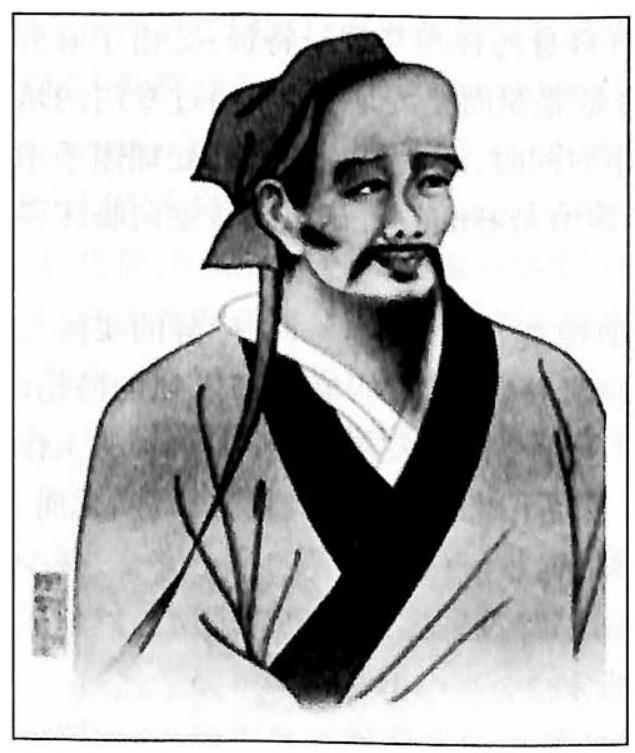
\includegraphics[max width=\textwidth]{2024_07_09_002a177993bd97d1d6d7g-026}
\end{center}

图 1-1 我国麻醉鼻祖一一华佗( 公元 200 年) (MGH) 公开演示在乙醚麻醉下行外科手术并获得成功(图 1-2),揭开了近代麻醉学的序幕。“麻醉” ( anesthesia)一词源于 1846 年 11 月 Oliver Wendell Holmes 给 Morton 的建议, 希腊语中 an 是 “没有”, 而 esthesia 是 “知觉” 的意思。近代麻醉学虽然只经历了 170 余年的历史, 但是, 由于社会的发展、人类的需求以及医学科学发展的驱动, 使得其迅猛发展。综观 170 余年的发展历史, 可将近代麻醉学的发展分为三个互相衔接而又各具特征的重要阶段。

\section*{(一)麻醉术 (anesthetic technique)}
这是近代麻醉学发展的第一阶段, 其时间跨度较长, 从 19 世纪 40 年代起大致经历了近 100 年的发展历程, 是麻醉学的起步阶段。

在这一发展阶段中, 麻醉工作者的主要任务是解决手术创伤所造成的疼痛, 即以无痛为目的, 为了能有效地控制疼痛, 麻醉工作的先驱们致力于药物和

\begin{center}
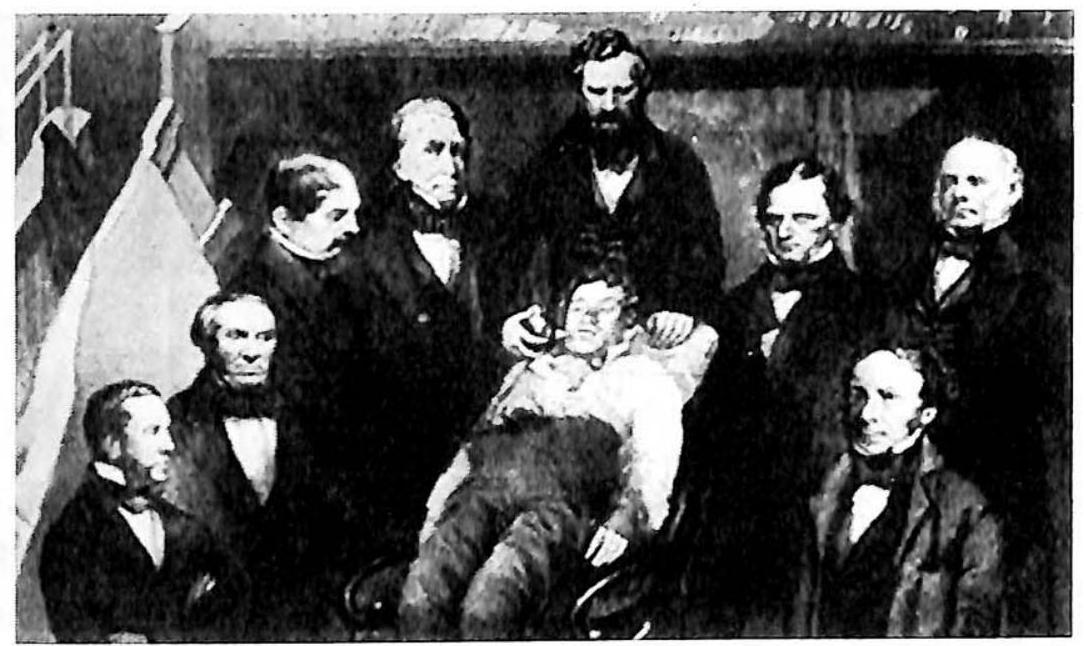
\includegraphics[max width=\textwidth]{2024_07_09_002a177993bd97d1d6d7g-027}
\end{center}

图 1-2 1846 年 10 月 16 日乙醚麻醉演示成功的场面

(或)麻醉方法的开发、创新和临床应用。继吸人麻醉后,还相继应用了局部麻醉及神经阻滞麻醉,诸如 Carl Koller 在 1884 年用可卡因滴眼进行表面麻醉, William Halsted 进行皮肤神经传导阻滞;1898 年 August Bier 应用可卡因进行蛛网膜下陁阻滞麻醉; 1911 年 G. Hirschel 用 $2 \%$ 普鲁卡因进行臂丛神经阻滞; 1921 年 Fidel Pages 应用普鲁卡因进行硬膜外阻滞等。在全身麻醉领域中,气管内插管成功应用于临床麻醉 (William Macewen,1878),便携式喉镜、紧闭式麻醉机以及 $\mathrm{CO}_{2}$ 吸收罐 (Ralph Waters,1923) 等相继问世。麻醉迅速风靡世界, 推动着外科学乃至整个医学的发展。但当时麻醉工作者的主要职责是掌握并使用这些技术。因此,麻醉学具有明显的医技科室特征。但这一发展阶段是十分重要的,因为它茲定了现代麻醉学的方法学基础,至今临床麻醉方法学仍以局部麻醉(含表面麻醉)、阻滞麻醉(包括神经阻滞、神经丛阻滞和椎管内阻滞)和全身麻醉为其三大重要内涵。与此同步,麻醉技术的发展与临床应用迫切要求麻醉工作者去解决许多相应的理论问题和临床实际问题,诸如解剖、生理、病理生理、并发症的防治等。因而积累和丰富了麻醉学的理论内容,麻醉学理论的发展不仅对临床实践起到指导作用,而且还是学科不断发展的重要基础。

\section*{(二)临床麻醉(clinical anesthesia)}
麻醉学发展的第二阶段时间跨度相对较短, 大约从 20 世纪 30 年代初至 50 年代末。其特点是:(1)由于第一阶段理论与技术的积累,使麻醉学初步具有自身的技术与理论特征; (2)由于麻醉技术的专业性以及保障患者安全的需要, 麻醉工作者不再是兼职而是专职, 必须经过专门的培训,已形成了麻醉专业队伍;(3)麻醉科医师在实施麻醉操作的同时,还要监测并早期处理因手术创伤、失血、并存疾病及麻醉本身引起的各种并发症, 临床诊治是麻醉学科从医技科室向临床科室发展的重要标志。

临床麻醉学具有六大组成部分, 即: (1)对患者进行术前检查、评估与准备; (2)麻醉的实施与管理;(3)专科患者的麻醉; (4)危重疑难患者的麻醉; (5)麻醉期间的监测; (6)麻醉并发症的防治。不难发现,在这一阶段中麻醉学已迅速地从医疗技术向临床诊治方面发展,麻醉工作者的工作领域已从术中拓展到围术期包括术前与术后, 临床麻醉除了为手术的顺利进行提供镇静、无痛、肌松、无不愉快记忆、合理控制应激及其他所必需的条件外,更要能保障患者的术中安全,减少并发症并促进患者术后顺利康复。麻醉学已具备明显的临床诊疗特征,因此也就理所当然地成为临床医学的重要组成部分, 即外科学中的一个重要分支学科。

在这一发展阶段中,麻醉学曾以其卓越的成就为推动外科学的发展而瞩目于世,诸如肌肉松驰药的临床应用(右旋筒箭毒碱, Harold R. Griffith 和 Enid Johnson,1942); 气管内插管和人工通气使胸外科能打开胸控禁区; 支气管麻醉技术 (Carlens 和 Bjork, 1950) 使“湿肺”患者获得安全\\
保障; 低温麻醉 (Bigelow,1950)的应用为阻断循环、打开心脏禁区进行心内直视手术奠定了基础。此外, 控制性降压及 “人工冬眠” 等也相继应用于临床。在麻醉学的支撑下, 外科学所属各专科如顾脑外科、心脏外科、胸外科、小儿外科等专科手术以及危重疑难患者的手术治疗均有迅猛的发展。为保障患者麻醉恢复期的安全,1951 年麻醉后恢复室 (recovery room,RR)正式成立。因此,临床麻醉是麻醉学趋于完善与成熟的重要发展阶段。

\section*{(三)麻醉学(anesthesiology)}
从 20 世纪 50 年代末至今, 麻醉学经历了又一次重要的飞跃。其特点是麻醉学在经历了 170 余年的发展, 特别是从 20 世纪 50 年代末以后 40 年的发展后, 通过长期的实践与开拓, 在其自身发展中不断地汲取着基础医学、临床医学、生物医学工程以及多种边缘学科中与麻醉学有关的理论与技术, 经发展形成了麻醉学自身的理论与技术体系, 从而成为临床医学中一个重要的二级学科。

从 20 世纪 50 年代开始, 发达国家医院对患者的管理提出 “分级治疗” 的新观念, 即将危重患者和重大手术患者集中管理, 并给予精良的设备及优秀的医护条件, 目的是提高危重患者的抢救成功率。在建立麻醉后恢复室取得成功经验的基础上,1958 年麻醉科第一个重症监测治疗病房( intensive care unit, ICU) 在美国建立, 从而将麻醉科工作领域从手术室拓展到病房及重症监护和治疗。不仅工作领域从手术室拓展到门诊与病房, 临床麻醉的工作重点也转移到对患者生命功能的监测、调节与控制。由 RR 发展起来的麻醉后苏醒室 (postanesthesia care unit,PACU )和麻醉科 ICU 的建立与管理已成为医院现代化的重要标志, 更为重大手术及重症患者的安全提供了强有力的保障。而疼痛诊疗工作的开展, 为麻醉学的理论与技术服务于疼痛患者开辟了新的途径, 麻醉学的印迹正走向医院的每个科室与角落。因此,临床麻醉、重症监测治疗及疼痛诊疗 (pain clinic) 已成为麻醉学的三个重要分支学科 (三级学科), 而围术期生命功能的调控则是麻醉学的精髓(图 1-3)。此外, 急救中心的工作, 药物依赖与戒断( “戒毒”)以及呼吸治疗等领域也越来越多地有赖于麻醉科医师的参与, 正在成为麻醉学的重要组成部分。正因为如此, “麻醉科” 的名称已越来越不能反映麻醉科工作的真正内涵。所以,当今世界有些国家已对麻醉科的名称进行修正, 如

\begin{center}
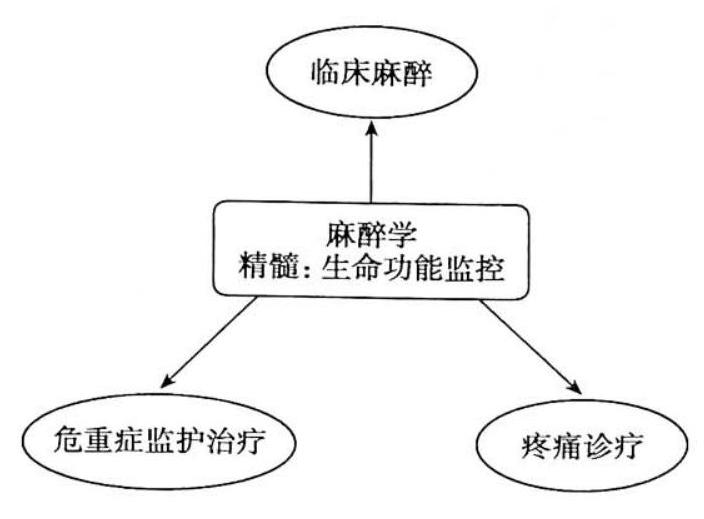
\includegraphics[max width=\textwidth]{2024_07_09_002a177993bd97d1d6d7g-028}
\end{center}

图 1-3 麻醉学的三个重要分支学科改称为麻醉复苏科 (department of anesthesiology and resuscitation)、麻醉与重症医学科 (department of anesthesiology and critical care medicine) 、麻醉与围术期医学科 (department of anesthesia and perioperative medicine) 等,为了突出当今麻醉学的突破性进展, 较多的出版物又将麻醉学冠以现代麻醉学 (modern anesthesiology) 的名称。

我国教育部和卫生部已分别下文将麻醉学归列为医学门类临床医学 (一级学科)之中, 明确是与内、外、妇产科等并列的二级学科, 是医院中一级临床诊疗科室。目前, 我国麻醉学科的建设与发展正在迅速向临床二级学科的平台前进。

\section*{第三节 麻醉科的组织结构与内满}
麻醉学属于临床医学中重要的二级学科, 麻醉科是医院中具有枢纽性的一级诊疗科室, 麻醉科主任在院长领导下工作。麻醉科的工作任务包括临床医疗、教育与科研等方面。一个符合二级学科内涵的麻醉科应由麻醉科门诊、临床麻醉 (含 PACU )、ICU、疼痛诊疗和实验室等部门组成。麻醉科的建设虽应根据医院规模及其所承担的工作任务不同而有所区别, 但各级医院均\\
应努力按二级学科的内涵加以健全与提高。

\section*{一、临床医疗工作}
\section*{(一)麻醉科门诊}
随着医院管理工作的进步, 特别是保证质量、提高效率和减轻患者负担, 麻醉科门诊 (或麻醉前评估中心) 将日益成为医院门诊工作的重要组成部分。麻醉科门诊的主要工作内容如下:

\begin{enumerate}
  \item 麻醉前检查、评估与准备 为缩短患者的住院周期 (床位周转率), 保证麻醉前充分准备, 凡拟接受择期手术的患者,在手术医师进行术前检查与准备的基础上, 人院前应由麻醉科医师在麻醉科门诊按要求作进一步的检查与准备。其优点是: (1)患者人院后即可安排手术, 甚至在当日即可安排手术, 可显著缩短住院日期, 提高床位周转率; (2)可避免因麻醉前检查不全面而延迟手术; (3)杜绝外科医师与麻醉科医师因对术前准备的意见不一致而发生矛盾; (4) 患者人院前麻醉科已能了解到病情及麻醉处理的难度, 便于恰当地安排麻醉工作。麻醉前检查、评估与准备工作目前均在病房进行, 随着医院现代化进程的加速, 有条件的医院应逐步将这一工作转移到门诊。

  \item 对麻醉并发症的随访和诊疗 麻醉后并发症由麻醉科医师亲自诊治是十分必要的。目前, 麻醉并发症的诊治并不是由麻醉科医师负责, 尤其是在患者出院后, 麻醉科医师无机会对这些患者进行诊疗, 疗效也不理想。随着麻醉科门诊的建立, 将改变这种状况, 对患者是有益的。

  \item 麻醉前会诊或咨询。

  \item 呼吸治疗、药物依赖戒断治疗 (“戒毒”)等。

  \item 疼痛诊疗可单独开设疼痛诊疗门诊或多学科疼痛诊疗中心,并可建立相应的病房。

\end{enumerate}

\section*{(二)临床麻醉}
临床麻醉的工作场所主要在手术室内, 目前已拓展到手术室外,其发展迅速,已成为临床麻醉的一个重要分支。手术室外麻醉广义是指病房手术室外的麻醉处理,包括门诊手术。狭义是门诊 (急诊) 及病房手术室外的麻醉、镇痛与镇静,包括介人治疗、内镜检查及各科无痛治疗等。在规模较大、条件较好的麻醉科,还应建立临床麻醉的分支学科 (或称为亚科),如心血管外科、胸外科、脑外科、产科和小儿外科麻醉等,以培养专门人才,提高专科麻醉的医疗质量。

\section*{1. 临床麻醉的主要工作内容}
(1)对患者进行术前检查、病情评估与准备。

(2)为手术顺利进行提供镇静、无痛、无不愉快记忆、肌松并合理控制应激反应等基本条件。

(3)提供完成手术所必需的特殊条件,如气管、支气管内插管, 控制性降压, 人工通气,低温及体外循环等。

(4) 对手术患者的生命功能进行全面、连续、定量的监测,并调节与控制在正常或预期的范围内,以维护患者的生命安全。应当指出,对患者生命功能进行监测与调控已是临床麻醉的精髓所在。因此, 麻醉科不仅必须配备有完备与先进的仪器及设备, 更要不断提高麻醉科医师的知识、素质与能力, 只有这样才能进行及时准确的判断与治疗。

(5) 建立 PACU 并进行科学管理,预防并早期诊治各种并发症, 确保患者术后顺利康复。

(6)积极创造条件,开展“手术室外麻醉”或“非住院患者的麻醉”, 以方便患者、节约医疗资源。但要有准备地实施,实施前必须建立相应的规范与制度,以确保患者安全。

(7) 开展术后镇痛工作,有条件的麻醉科应建立术后镇痛信息管理系统及信息资料数据库。

(8)建立麻醉科信息管理系统,强化科学管理,以提高医疗质量和工作效率。

\begin{enumerate}
  \setcounter{enumi}{1}
  \item 临床麻醉常用方法 临床麻醉的方法 (技术)和药物虽然众多,根据麻醉药作用于神经系统的不同部位,可分为局部(区域)麻醉和全身麻醉两大类(表1-1)。
\end{enumerate}

表 1-1 临床麻醉基本方法分类

\begin{center}
\begin{tabular}{|c|c|c|c|}
\hline
分 类 & 麻 醉 方 法 & 麻醉药给药方式 & 麻醉药作用的部位 \\
\hline
\multirow[t]{2}{*}{全身麻醉} & 吸人全麻 & \begin{tabular}{l}
经呼吸道吸人 \\
静脉注射 \\
\end{tabular} & 中枢神经系统 \\
\hline
 & 静脉全麻 & \begin{tabular}{l}
肌内注射 \\
直肠灌注 \\
\end{tabular} &  \\
\hline
局部(区域)麻醉 & \begin{tabular}{l}
蛛网膜下隙阻滞 \\
硬膜外阻滞 \\
神经干 (丛) 阻滞 \\
局部浸润麻醉 \\
\end{tabular} & \begin{tabular}{l}
局麻药注人蛛网膜下隙 \\
局麻药注人硬脊膜外隙 \\
局麻药注人神经干(丛) \\
局麻药局部浸润 \\
\end{tabular} & \begin{tabular}{l}
蛛网膜下脊神经 \\
硬脊膜外脊神经 \\
神经干 (丛) \\
皮肤、黏膜神经末梢 \\
\end{tabular} \\
\hline
\end{tabular}
\end{center}

目前已较少使用单一的药物或单一的方法进行麻醉, 临床上使用较多的是复合麻醉或称平衡麻醉 (balanced anesthesia)和联合麻醉 (combined anesthesia)。复合麻醉系指同时使用两种或两种以上麻醉药和(或)辅助药物以达到麻醉的基本要求,以能减少单个药物的用量及副作用,例如使用镇静、麻醉镇痛与肌肉松驰药进行静脉复合全麻。联合麻醉系指同时使用两种或两种以上方法以达到麻醉的基本要求, 以能取长补短、综合发挥各种方法的优越性, 例如全身麻醉与硬膜外阻滞联合应用等。

\section*{(三)麻醉后苏醒室(postanesthesia care unit,PACU)}
PACU 是手术结束后继续观察病情, 预防和处理麻醉后近期并发症, 保障患者安全, 提高医疗质量的重要场所。PACU 应配备有专门的护士与医师管理患者, 待患者清醒、生命体征稳定后即可送回病房。PACU 可有效预防麻醉后早期并发症, 杜绝恶性医疗事故, 还可缩短患者在手术室停留时间, 提高手术台利用率, 是国际、国内成功而又成熟的经验。若患者病情不稳定, 如呼吸、循环功能障碍者应及时送人 ICU。

\section*{(四)麻醉科 ICU}
是指由麻醉科主管的 ICU, 主要针对手术后患者, 是围术期危重病诊治、保障重大手术安全、提高医疗质量的重要环节, 是现代高水平、高效益医院的必然产物。ICU 的特点是: (1)配备有先进的设备以能对患者生命功能进行全面、连续和定量的监测; (2)具备早期诊断及先进的治疗设备与技术; (3)采用现代化管理,因而具有高工作效率和抢救成功率; (4)拥有一支训练有素的医疗护理队伍。

进人 ICU 的患者由麻醉科医师和手术医师共同负责, 麻醉科医师的主要任务是: 对患者进行全面、连续、定量的监测; 维护患者的体液内稳态 (homeostasis); 支持循环、呼吸等功能的稳定;防治感染;早期诊治各种并发症及营养支持等。手术医师侧重于原发病和专科处理。待患者重要脏器功能基本稳定后即可转回原病室。

\section*{(五)疼痛诊疗}
疼痛诊疗是麻醉科工作的重要组成部分。鉴于疼痛的多学科性及麻醉科的工作特性, 麻醉科疼痛诊疗以急性疼痛诊疗为基础、慢性疼痛诊疗为特色。麻醉科疼痛诊疗的工作内容主要包括:术后止痛及急性疼痛的诊疗,慢性疼痛的诊疗,无痛诊疗乃至无痛医院是麻醉科的重任。在进行慢性疼痛诊疗时, 应当强调疼痛诊疗的多学科性和临床诊断的重要性, 因此, 从事慢性疼痛诊疗医师必须有扎实的、相关科室的临床诊疗功底,必须具有麻醉科主治医师的资格再经专业培训后才能胜任。

\section*{二. 科 研 工 作}
科学研究是麻醉科的重要工作内容,学科内涵建设要以临床为基础、科研为先导、教育为根本。科研工作要明确研究方向、制订计划、组织实施、定期总结。科研工作要特别注意两个问题,一是要树立 “临床工作向前一步就是科研” 的意识,即在日常工作中要做有心人,善于提出问题,注意选准主题,通过研究、创新去解决问题,要完善记录、积累资料,统计分析,并撰写论文。二是要努力使麻醉学研究从指标依赖性向思维依赖性发展, 要从依赖指标切实转变到依赖思维,思维的核心是创新,思维的方式是实践-理论-再实践,要产、学、研相结合。这是提高临床医疗水平和麻醉科学术地位的重要途径。在有条件的医院麻醉科可成立麻醉学实验室或麻醉学研究室。麻醉科成立研究室(或实验室)时,麻醉科主任(或副主任)应兼任研究室(或实验室)主任。成立研究室(或实验室)时必须具备以下基本条件:

\begin{enumerate}
  \item 要有学术水平较高, 治学严谨, 具有副教授或副主任医师以上职称的学科或学术带头人;

  \item 形成相对稳定的研究方向并有相应的研究课题或经费;

  \item 配备有开展研究所必需的专职实验室人员和仪器设备;

  \item 要形成一支结构合理的人才队伍, 主要包括研究骨干、研究人员、技术人员和管理人员。

\end{enumerate}

\section*{三、教育工作}
21 世纪初期我国医学教育的目标是建立包括学校基础教育( basic education, BE)、毕业后教育 (postgraduate education, PGE) 和继续医学教育 (continuous medical education, CME) 在内的连续统一的终生医学教育体系, 麻醉学科也不例外。BE 主要是《麻醉学》在临床医学专业独立授课和研究生教育,《麻醉学》独立开课是医学生知识结构的需要, 是学校基础教育与毕业后教育衔接的需要, 是麻醉学二级学科建设与发展的需要。PGE 指住院医师培训, 或称规范化住院医师培训,即大学本科毕业后再经 3 年的住院医师培训 (“ $5+3$ ”或“7+2”模式); CME 主要针对主治医师以上人员。这是提高麻醉科医师素质与水平的重要途径, 应努力使之不断规范化、制度化、法律化。为能在我国更好地推动 ICU 和疼痛诊疗工作的开展, 应积极创造条件, 实施 ICU 及疼痛诊疗医师的培训和准人制度。医学院 (校)附属医院应积极创造条件成立麻醉学教研室, 有多所附属医院的医学院校可以成立麻醉学系,以能统一组织完成上述任务。

\section*{第四节 学好麻醉学}
为了在医学院校临床医学专业学生中做好麻醉学的基础教育, 本课程的内容除扼要叙述麻醉学的基本技术和方法外,重点介绍: (1)对人体生命功能的监测、调节与控制, 诸如气道管理以及呼吸、氧供需平衡、血流动力学及体液平衡的监控等; (2)休克、ALI 及 ARDS、MODS 和心肺脑复苏等危重患者的急救和诊治知识; (3)疼痛诊疗及药物依赖与戒断的基本知识。应当指出, 这些内容是做好一个临床医师必备的共同基础, 因此, 是医学生知识结构的需要, 更是医学生进人临床各专科后进一步发展的基础与需要, 是临床医师对患者诊疗的宏观调控、应急能力以及对危重患者诊治能力的重要基础。要认真学习, 重在理解, 注意与相关课程之间的联系与沟通, 以能举一反三。

应当强调,我国麻醉学科近 20 年已取得长足的进步,但发展很不平衡,就整体而言, 学科目前正处于从三级学科向二级学科平台发展的重要阶段,相信通过努力我国麻醉学将迅速进人国际先进平台。

\section*{第二章手术患者术前病情评估与准备}
手术患者术前病情评估是保障手术患者安全的重要环节。术前病情评估不仅对麻醉科医师, 而且对手术科室医师都是至关重要的工作。其意义涉及保障患者麻醉和手术中的安全, 以及减少围术期并发症的发生率和病死率。多数麻醉药对机体的重要生命器官和系统的功能, 例如呼吸、心血管系统等都有非常明显的影响。麻醉药的治疗指数 (半数致死量/半数有效量)仅为 $3 \sim 4$ 。相比之下, 大多数非麻醉药的治疗指数却是数百甚至数千。麻醉药这么窄的安全范围, 说明了麻醉自身的风险性, 然而更重要的方面是来自患者的病情和手术的复杂性, 以及患者对麻醉和手术的承受能力。因此, 麻醉的危险性、手术的复杂性和患者的承受能力是麻醉前病情评估的要点。

麻醉的诞生是外科学发展的里程碑, 现代麻醉学的发展极大地推动和保障了外科学的进步。一个普通的外科手术患者可能会并存有严重的内科疾病, 例如心脏病、高血压、糖尿病等。随着老龄化社会的到来, 百岁老人做手术已不再是稀奇事。科学发展到今天, 许多过去认为是手术的禁忌证, 如今却因为能够改善器官功能成为手术的适应证, 如急性心肌梗死的患者做急诊冠状动脉搭桥术, 晚期严重的慢性阻塞性肺疾病的患者做肺减容手术, 终末期器官功能衰竭的患者行器官移植手术等。外科已几乎无手术禁忌证可言。然而面对这样的手术却给麻醉带来极大的风险和挑战。

手术患者术前病情评估与准备 (preoperative evaluation and preparation)工作包括: (1)全面了解患者的全身健康情况和具体病情; (2)评估患者接受麻醉和手术的耐受性; (3)明确各脏器疾病和特殊病情的危险所在, 术中可能会发生哪些并发症, 需采取哪些防治措施; (4)选择麻醉前用药和麻醉方法, 拟订具体麻醉实施方案和麻醉器械准备。为了切实做好术前病情评估和准备工作,要求: (1)充分认识手术患者术前病情评估与准备的重要性; (2)了解麻醉前访视与检查的流程; (3)对麻醉前准备的特殊性有初步概念; (4)掌握麻醉前用药原则。

\section*{第一节 术前访视与术前病情评估门诊}
\section*{(一)麻醉科医师手术前访视}
目前在国内, 对大多数患者通常都是在手术日前一天, 接到外科手术通知后, 麻蟀科医师进行手术前访视。对于高危和有特殊情况的患者, 外科医师于手术日前几天请麻醉科医师会诊,必要时进行多学科术前讨论。因此, 术前访视的时间受到患者基础疾病、手术种类以及医疗体制的影响。

麻醉科医师手术前访视的流程主要包括: 复习病历, 察看各项术前实验室检查, 访视患者了解麻醉相关病史和进行各系统回顾, 进行体格检查和对重要系统进行功能测试, 最后对患者做出麻醉和手术风险评估和判断, 制订出围术期麻醉计划。向患者和患者家属交代病情、麻醉方式和手术麻醉的风险以及必要的术前准备,如术前禁食等,并签署麻醉知情同意书。

为保证麻醉科医师的术前访视, 外科医师需要在术前完成所有必要的准备和检查。患者人院后各项术前实验室检查一般需要 $2 \sim 3$ 天才能回报, 因此患者在手术前需要等待约一周时间,明显延长住院时间。

在国际上, 随着日间手术的发展, 快通道和缩短住院时间、平均住院天数, 加强病房床位周转率等方面的需求, 手术患者, 即便是冠状动脉旁路移植术, 往往是手术当天人院, 人院后即手\\
术, 术后视病情和恢复情况决定留观和住院。这就使手术前评估的时机发生了很大变化, 要求患者于手术前在门诊完成术前检查和评估。因此, 麻醉科手术前病情评估门诊应运而生。手术前病情评估门诊的开展, 使发达国家的普通外科手术平均住院天数减为 $3 \sim 4$ 天、神经外科和心脏外科手术的平均住院天数为 $6 \sim 8$ 天。等于在不增加投资或仅增加少量投资的情况下, 增加了医疗资源。

\section*{(二)麻醉科手术前病情评估门诊}
麻醉科手术前病情评估门诊在我国仅在少数医院刚刚起步。麻醉科术前评估门诊的建立和工作是为了医院和医疗工作发展的需要, 离不开医院和各学科的支持。外科医师对门诊就诊准备择期手术的患者, 完成必要的常规检查和专科检查后, 在决定人院前建议患者去麻醉科手术前病情评估门诊就诊。麻醉科门诊通常由资深的麻醉科医师负责,根据患者的病史、体格检查、化验和辅助检查等结果, 对患者耐受麻醉的情况进行评估。对于化验和辅助检查不全的患者, 针对其具体疾病要求进一步完善相关检查。对于合并症控制不理想的患者, 建议到相关科室会诊,以调整治疗方式和药物剂量。最后向患者解释相关手术可能采取的麻醉方式。完成一份简单的术前病情评估病历或评估表, 并列出该患者的主要问题。患者人院当天, 负责麻醉的医师通过复习患者的术前病情评估病历或评估表, 并询问患者一些基本情况,一目了然患者的具体病情,选择合适的麻醉方式和监测方法,以保证麻醉的安全性。

开设麻醉评估门诊除了减少住院时间、加快床位周转等作用外,更重要的是对伴有合并症的患者在术前进行了系统全面的检查, 并得到及时治疗和良好控制。患者人院后可以当天或尽快安排手术; 避免因合并症控制不良, 或术前检查结果不全, 而推迟手术; 也提高了手术麻醉的安全性。美国圣路易斯华盛顿大学医院开设麻醉科术前病情评估门诊以来, 已达到 $80 \%$ 的择期手术患者都经过术前评估门诊, 避免了因故而推迟手术的情况。此外, 患者可以在住院前对麻醉有初步了解,以减少对麻醉的恐惧感和不必要的担心。

\section*{第二节 手术前病情评估的流程和方法}
\section*{一、手术前病情评估的流程}
\begin{enumerate}
  \item 复习病历 (史) 麻醉前病情评估首要的是从病历中获得足够的病史, 主要包括外科疾病和手术情况, 以及并存的内科疾病和治疗情况。
\end{enumerate}

外科情况要了解外科疾病的诊断, 手术的目的, 部位、切口, 切除脏器范围, 手术难易程度,预计出血程度, 手术需时长短和手术危险程度, 以及是否需要专门的麻醉技术 (如低温、控制性降压等)。

内科情况要了解患者的个人史、既往史、以往手术、麻醉史和治疗用药史。明确并存的内科疾病及严重程度, 当前的治疗情况, 近期的检查结果, 是否需要进一步做有关的实验室检查和特殊的功能测定。必要时请有关专科医师会诊, 协助评估有关器官功能状态, 商讨进一步手术准备措施。

\begin{enumerate}
  \setcounter{enumi}{1}
  \item 分析各项术前检查和化验结果 择期手术患者通常要进行一系列常规的术前检查(表 2-1)。但是哪些是术前必需或常规的检查与化验项目, 目前并无统一定论和指南。通常人院患者在手术前完成血、尿、粪三大常规化验, 出凝血时间,血生化(肝、肾功能)检查,心电图以及感染疾病方面的检查(如乙型病毒性肝炎、HIV 等)。对合并有内科疾病者,根据病情做进一步检查:胸部 X 线检查、肺功能测定、动脉血气分析、心功能测定, 以及必要的专科检查和化验。其目的是有助于医务人员对患者的病情有全面或充分的了解, 以便做出正确的评估,降低影响麻醉管理的不利因素,增加手术和麻醉的安全性。\\
表 2-1 手术患者术前进行实验室和特殊检查的标准 (最低标准)
\end{enumerate}

\begin{center}
\begin{tabular}{ll}
\hline
必需检查项目 & 1. 血常规 包括血小板计数,有条件加做血细胞比容(Hct) \\
2. 尿常规 包括镜检及尿比重 &  \\
3. 苼常规 &  \\
4. 肝功能 包括血浆蛋白、胆色素、转氨酶测定 &  \\
5. 肾功能 包括血尿素氮(BUN)和血肌酎(Cr)测定 &  \\
6. 感染疾病方面的检查 主要包括 HBV、HIV 等的相应检查 &  \\
7. 凝血机制 包括凝血酶原时间 (PT)、部分凝血活酶时间 (APTT) 和纤维蛋 &  \\
白原含量 &  \\
\end{tabular}
\end{center}

\begin{enumerate}
  \setcounter{enumi}{2}
  \item 术前访视和检查 麻醉科医师术前应访视患者,从麻醉科医师的角度进一步了解患者与麻醉可能相关的病史,并进行系统问诊和体检,往往可以获得十分重要的第一手资料。同时可以帮助患者了解有关麻醉的问题, 消除紧张、焦虑情绪,建立良好的医患关系。如果患者是小儿,应重视帮助患儿及家长对手术麻醉做好心理上的准备。
\end{enumerate}

体检主要是检查患者的生命体征,观察患者的全身情况。系统问诊的重点是心血管系统、呼吸系统、神经系统、凝血、肝功能、肾功能和内分泌系统。所有这些术前检查的最终目的是对患者做出麻醉和手术风险的判断。

\begin{enumerate}
  \setcounter{enumi}{3}
  \item 进行麻醉和手术风险判断根据麻醉前访视的结果对手术、麻醉的风险进行综合分析。美国麻醉医师协会 (American Society of Anesthesiologists, ASA)颁布的患者全身体格健康状况分级是目前临床麻醉较常采用的评估分级方法之一, 其分级标准见表 2-2。I、II 级患者的麻醉耐受性一般均良好, 麻醉经过平稳; III级患者对接受麻醉存在一定的危险, 麻醉前需尽可能做好充分准备,对麻醉中和麻醉后可能发生的并发症,要采取积极有效的预防措施; IV 、V 级患者的麻醉危险性极大,充分、细致的麻醉前准备尤为重要。
\end{enumerate}

表 2-2 ASA 麻醉病情评估分级

\[
\begin{aligned} & 分级 \multicolumn{1}{c}{ 标 准 } \\ & I 级 无器质性疾病,发育、营养良好,能耐受麻醉和手术 \\ & II 级 心、肺、肝、肾等实质器官虽然有轻度病变,但代偿健全,能耐受一般麻醉和手术 \\ & III级 心、肺、肝、肾等实质器官病变严重,功能减低,尚在代偿范围内,对麻醉和手术的耐受稍差 \\ & IV级 上述实质器官病变严重,功能代偿不全,威胁着生命安全,施行麻醉和手术需冒很大风险 \\ & V 级 病情危重,随时有死亡的威胁,麻醉和手术非常危险 \end{aligned}
\]

注:如系急症,在每级数字前标注“急”或“ $E$ (emergency)”字

\begin{enumerate}
  \setcounter{enumi}{4}
  \item 知情同意 知情同意是术前评估的必要内容,已经成为不可缺少的法律文书。向患者解释治疗或诊断性操作的副作用、危险性及并发症后, 患者认可并签字, 就获得了知情同意。目的是向患者提供使其做出合理选择所需要的信息。解释麻醉计划和可能的并发症对于建立患者与医师之间的良好关系是非常重要的, 并且可以预防以后可能发生的纠纷。某些情况下, 只能\\
由患者亲属或被授权人签署知情同意书。
\end{enumerate}

\section*{二、手术前病情评估的方法}
\section*{(一)总体评估方法}
手术前病情评估既是科学也是艺术。经验丰富的麻醉科医师能迅速抓住一些要点,做出基本评估判断。包括患者的自身条件、全身情况、有无合并症及严重程度、重要的脏器功能和外科手术的复杂性等。

\begin{enumerate}
  \item 患者的自身条件 随着我国已步人老龄化社会,患者的年龄成为重要的麻醉风险因素。患者实施的手术可能是一般手术, 但是如果是一高龄患者, 其麻醉的风险性较年轻者要高得多。

  \item 全身情况 对判断其对麻醉的耐受性非常重要,如精神状态、发育、营养、有无贫血、脱水、水肿、发绀、发热、过度消瘦或肥胖症等。

  \item 并存疾病及器官功能 患者实施的可能是普通手术, 但是如果并存一种或多种疾病, 就会使麻醉的风险性增加,如合并有心脏病、糖尿病、慢性阻塞性肺疾病等。然而即便是高龄患者, 又并存多种疾病, 其对麻醉的耐受性主要取决于重要生命器官的功能状态, 特别是心、肺功能的代偿与好坏。所以在系统评估中,重点是呼吸系统和心血管系统。

  \item 外科手术的复杂性 看似不属于患者的病情范畴,但却与病情息息相关。麻醉的风险性与手术大小并非完全一致,复杂的手术可使麻醉的风险性明显增加, 而有时手术并不复杂,但患者的病情和并存疾病却为麻醉带来更多风险。手术复杂、手术时间长、出血量大等因素都显著增加患者麻醉和手术的风险性。然而, 有的手术虽然复杂, 但可以改善或恢复患者的器官功能, 如冠状动脉搭桥术、肺减容术、器官移植术等, 这无疑给术前病情评估带来了新的挑战。

\end{enumerate}

\section*{(二)心血管风险的评估}
对非心脏手术的患者要注意有无心血管方面的疾病, 如先天性心脏病、心脏瓣膜病、冠状动脉硬化性心脏病、心肌病、大血管病, 以及高血压和心律失常。与麻醉风险相关的主要是心功能状态, 以及某些特别的危险因素, 例如, 不稳定性心绞痛、近期 ( $<6$ 个月) 心肌梗死、致命性心律失常等。术前心功能好往往反映患者有较强的代偿能力和对手术麻醉的承受能力。超声心动图检查除可以提供心内解剖结构的变化外, 还可以评估心室功能。其中最重要的一个指标是心室射血分数 $(\mathrm{EF})$ 。如 $\mathrm{EF}<50 \%$ 属中度危险患者, $\mathrm{EF}<25 \%$ 则为高度危险患者。

\begin{enumerate}
  \item 床旁试验方法 麻醉科医师可以通过一些简易的床旁试验来判断患者当前的心肺储备能力:
\end{enumerate}

(1) 屏气试验 (breath holding test): 先让患者做数次深呼吸,然后在深吸气后屏住呼吸,记录其能屏住呼吸的时间。一般以屏气时间在 30 秒以上为正常; 屏气时间短于 20 秒, 可认为其心肺功能属显著不全。

(2)爬楼梯试验:患者能按自己的步伐不弯腰爬上三层楼,说明心肺储备能力尚好,围术期发病率和死亡率明显低。

(3) 6 分钟步行试验: 一个定量分析心肺功能的方法。测量运动期间最大耗氧量 (maximal oxygen consumption, $\left.\mathrm{VO}_{2} \mathrm{max}\right)$ 是判断患者开胸后是否发生肺部并发症的一个准确的术前评估方法。如果患者 $\mathrm{VO}_{2} \max \geqslant 20 \mathrm{ml} /(\mathrm{min} \cdot \mathrm{kg})$, 肺部并发症少; $\mathrm{VO}_{2} \max \leqslant 10 \mathrm{ml} /(\mathrm{min} \cdot \mathrm{kg})$ 时, 有高危险性, 短期内死亡率大于 $30 \%$ 。6 分钟步行试验和 $\mathrm{VO}_{2}$ max 有很好的相关性。如果患者 6 分钟的步行距离达到 $360 \mathrm{~m}$, 则 $\mathrm{VO}_{2} \mathrm{max}$ 大约是 $12 \mathrm{ml} /(\mathrm{min} \cdot \mathrm{kg})$; 若 6 分钟的步行距离小于 $660 \mathrm{~m}$, 表明 $\mathrm{VO}_{2}$ max 小于 $15 \mathrm{ml} /(\mathrm{min} \cdot \mathrm{kg})$ 。

\begin{enumerate}
  \setcounter{enumi}{1}
  \item Goldman 心脏危险指数( cardiac risk index, CRI) 已在临床麻醉中应用达 30 年,虽然有些争论, 但仍为评估围术期心脏风险性的依据(表 2-3), CRI 愈高其心脏危险性愈大( 表 2-4)。\\
在总分 53 分中, 有 28 分是经过积极的术前准备和治疗而可能得以纠正的, 如心力衰竭、心律失常、低氧血症等,病情改善后可使麻醉和手术的风险性降低。
\end{enumerate}

表 2-3.Goldman 心脏危险指数评估

评价项目

指数分

\begin{enumerate}
  \item 病史
\end{enumerate}

(1) 年龄>70 岁

(2) 最近 6 个月内出现心肌梗死

\begin{enumerate}
  \setcounter{enumi}{1}
  \item 心脏检查
\end{enumerate}

(1)存在舒张期奔马律或颈静脉怒张 11

(2)明显的主动脉瓣狭窄

\begin{enumerate}
  \setcounter{enumi}{2}
  \item 心电图
\end{enumerate}

(1)非窦性心律或房性期前收缩 7

(2)室性期前收缩>5 次/分 7

\begin{enumerate}
  \setcounter{enumi}{3}
  \item 病情危重者(有下列任何一项) 3
\end{enumerate}

$\mathrm{PaO}_{2}<60 \mathrm{mmHg}$ 或 $\mathrm{PaCO}_{2}>50 \mathrm{mmHg}$

血清 $\mathrm{K}^{+}<3.0 \mathrm{mmol} / \mathrm{L}$ 或 $\mathrm{HCO}_{3}^{-}<20 \mathrm{mmol} / \mathrm{L}$

BUN>17. $85 \mathrm{mmol} / \mathrm{L}$ 或>50mg $/ \mathrm{dl}$ (正常为 $2.5 \sim 8.0 \mathrm{mmol} / \mathrm{L}$ 或 $7 \sim 22 \mathrm{mg} / \mathrm{dl}$ )

$\mathrm{Cr}>265.2 \mu \mathrm{mol} / \mathrm{L}$ 或 $>3 \mathrm{mg} / \mathrm{dl}$ (正常为 $45 \sim 120 \mu \mathrm{mol} / \mathrm{L}$ 或 $0.5 \sim 1.4 \mathrm{mg} / \mathrm{dl}$ )

ALT 异常, 有慢性肝病征象

\begin{enumerate}
  \setcounter{enumi}{4}
  \item 实施手术
\end{enumerate}

(1)腹腔内、胸腔内或主动脉手术 3

(2)急诊手术 4

表 2-4 不同的 CRI 分级和死亡率

\begin{center}
\begin{tabular}{ccc}
\hline
分级 & CRI 分 & 心脏原因死亡率 (\%) \\
\hline
I & $0 \sim 5$ & $0.3 \sim 3$ \\
II & $6 \sim 12$ & $1 \sim 10$ \\
III & $13 \sim 25$ & $3 \sim 30$ \\
IV & $26 \sim 53$ & $19 \sim 75$ \\
\hline
\end{tabular}
\end{center}

\begin{enumerate}
  \setcounter{enumi}{2}
  \item 对冠心病患者的风险评估 对冠心病患者进行围术期风险评估通常基于三个基本要素: (1)患者存在的风险因素;(2)患者的功能状态;(3)手术存在的风险因素。应根据三者各自的风险程度,对患者围术期的风险性进行综合评估。
\end{enumerate}

(1)患者存在的风险:(1)高危风险因素:新发心肌梗死 ( $<6$ 周),不稳定心绞痛,心肌梗死后仍存在的心肌缺血, 缺血性及充血性心力衰竭, 严重心律失常, 近 40 天内接受冠脉再血管化术等。高危患者只适合进行急诊或挽救患者生命的手术。(2) 中危风险因素: 近期发生心肌梗死 ( $>6$ 周且 $<3$ 个月) 而未遗留后遗症或处于危险状态的心肌, 在药物控制下的稳定性心绞痛 ( I ~II 级), 既往发生过围术期缺血性事件, 糖尿病, 心脏射血分数低 ( EF<0.35), 心力衰竭代偿期。(3)低危风险因素: 年龄 $\geqslant 70$ 岁, 高血压, 左心室肥厚, 6 年内施行过冠状动脉旁路移植术 (CABG)或经皮冠状动脉腔内成形术(PTCA)且未残留心肌缺血症状。

(2)患者的功能状态: 通常以其对体力活动的耐受能力来评价。运动耐量试验 (exercise tolerance test) 是评估患者围术期风险的一个重要方法。蹬车运动试验中,低耐量运动 (心率< 100 次/分)即产生心肌缺血者为高危患者;大运动量时 (心率>130 次/分)仍无缺血表现者为低\\
危患者。不能持续走上两层楼梯者,术后发生心肺并发症者占 $89 \%$ 。患者对活动的耐受能力还可以代谢当量 (metabolic equivalent of task, METs) 表示, $1 \mathrm{MET}$ 大约耗氧 $3.5 \mathrm{ml} /(\mathrm{kg} \cdot \mathrm{min})$ 。根据患者平常的活动能力可间接判断其耗氧量, 从而评价其对麻醉、手术的耐受性(表 2-5)。功能状态评估: $>10 \mathrm{METs}$ 为极好, $7 \sim 10 \mathrm{METs}$ 为好, $4 \sim 7 \mathrm{METs}$ 为中等, $<4 \mathrm{METs}$ 为差。研究发现, 若患者活动量低于 $4 \sim 5$ 个代谢当量, 围术期易发生各种并发症。对于功能状态良好者, 任何进一步检查的结果都很少会改变治疗方案,可按原计划手术。

表 2-5 代谢当量评估表

\begin{center}
\begin{tabular}{cl}
\hline
代谢当量(METs) & \multicolumn{1}{c}{患者活动能力} \\
\hline
1 & 能自己进食,穿衣,看电脑、上网 \\
2 & 能室内步行,或下楼,或胜任烹调 \\
3 & 能步行 $1 \sim 2$ 个街区 \\
4 & 能完成花园修剪、除草等工作 \\
5 & 能爬一层楼梯,或跳舞,或骑自行车 \\
6 & 能打高尔夫球 \\
7 & 能胜任单打网球 \\
8 & 快速爬楼梯,慢跑 \\
10 & 慢速跳绳或骑独轮车 \\
11 & 能快速游泳、跑步 \\
12 & 能滑雪或打满场篮球 \\
\hline
\end{tabular}
\end{center}

(3) 手术存在的风险: (1)高风险手术: 器官移植手术, 特别是心、肺、肝、胰的移植手术; 主动脉和大血管手术以及外周血管手术; 浈腔内大手术以及持续时间较长的手术 (易致体内体液转移) 等。(2)中度风险手术: 头颈部手术; 胸腔内或腹腔内手术; 颈内动脉内膜切除术; 矫形外科手术;前列腺手术等。(3)低风险手术:体表部位手术;乳腺手术;扁桃体切除; 白内障手术等。

此外, 近期研究表明, 术前肌酎水平高于 $176.8 \mu \mathrm{mol} / \mathrm{L}(2 \mathrm{mg} / \mathrm{dl})$ 是大型非心脏手术术后发生心脏并发症的一项独立危险因素。与没有肾脏疾病的患者比较, 患有肾脏疾病, 如术前血肌酎水平 $>124 \mu \mathrm{mol} / \mathrm{L}(1.4 \mathrm{mg} / \mathrm{dl})$, 是术后发生肾功能不全和增加远期发病率及死亡率的危险因素。

\section*{(三)呼吸功能的评估}
\begin{enumerate}
  \item 危险因素 术后肺部并发症在围术期死亡原因中仅次于心血管居第二位。其危险因素包括: (1)肺功能损害程度; (2)慢性肺部疾病, 术后呼吸衰竭的危险性增加; (3)并存中至重度肺功能不全,行胸部和上腹部手术者; (4) $\mathrm{PaO}_{2}<60 \mathrm{mmHg}, \mathrm{PaCO}_{2}>45 \mathrm{mmHg}$ 者; (5)有吸烟史; (6)有哮碝史; (7)有支气管肺部并发症。
\end{enumerate}

\section*{2. 评估方法}
(1)一般评估方法: 可根据相关病史和体征排除有无呼吸道的急、慢性感染; 有无哮喘病史, 是否属于气道高反应性 (airway hyperresponsiveness) 患者; 对于并存有慢性阻塞性肺疾病 (COPD)的患者, 术前需通过各项检查, 如胸部影像学检查、肺功能试验 (pulmonary function testing)、血气分析(blood gas analysis) 等, 来评估患者的肺功能。

(2) 肺功能的评估:术前对患者肺功能的评估十分重要, 特别是原有呼吸系统疾病, 或需进行较大手术, 或手术本身可进一步损害肺功能者, 肺功能评估显得更为重要。对肺功能的评估可为术前准备及术中、术后的呼吸管理提供可靠的依据。尽管现代检测肺功能的方法甚多且日\\
益先进, 但在常规测定中最重要的仍是一些最基本的指标 (图 2-1)。例如, 肺活量低于预计值的 $60 \%$ 、通气储备百分比 $<70 \%$ 、第一秒用力呼气量与用力肺活量的百分比 $\left(\mathrm{FEV}_{1.0} / \mathrm{FVC} \%\right)<60 \%$或 $50 \%$,术后有发生呼吸功能不全的危险。当 $\mathrm{FVC}<15 \mathrm{ml} / \mathrm{kg}$ 时, 术后肺部并发症的发生率常明显增加。最大通气量(MVV) 也是一项有价值的指标。一般以 MVV 占预计值的 $50 \% \sim 60 \%$ 作为手术安全的指标, 低于 $50 \%$ 为低肺功能, 低于 $30 \%$ 者一般列为手术禁忌证。对于有可能做全肺切除者最好能行健侧肺功能测定或分侧肺功能测定。动脉血气分析简单易行, 可以了解患者的肺通气功能和换气功能。

\begin{center}
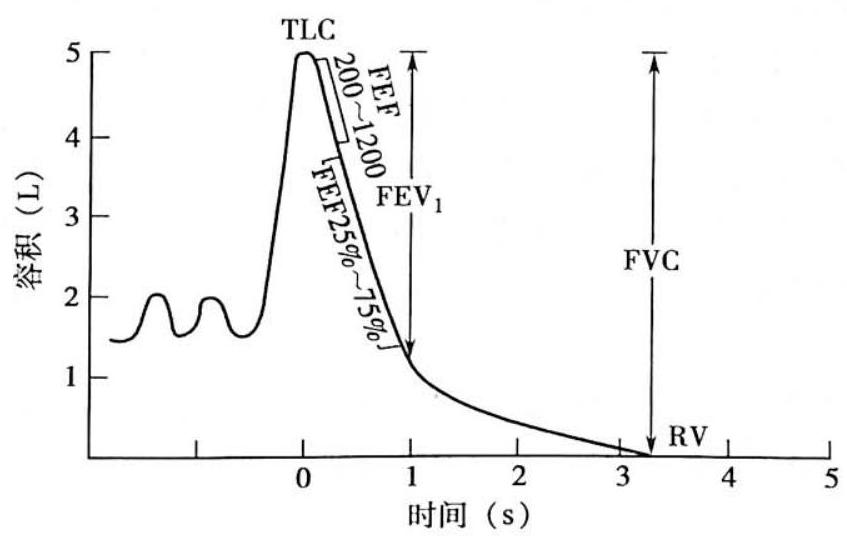
\includegraphics[max width=\textwidth]{2024_07_09_002a177993bd97d1d6d7g-038}
\end{center}

图 2-1 肺功能曲线图

(3)手术部位的影响: 评估术后发生肺部并发症的危险时,手术部位十分重要。切口邻近膈肌时风险增加; 上腹部手术和剖胸手术发生术后呼吸系统并发症的风险性最大, 为 $10 \%$ $40 \%$ 。上腹部手术后功能残气量和肺活量降低, 可持续 5 7 天。非胸、腹部手术术后呼吸系统并发症相对较少。

此外, 睡眠呼吸暂停综合征患者的围术期麻醉管理尤其是气道管理非常困难。睡眠呼吸暂停综合征的定义为睡眠期间反复发作的阻塞性呼吸暂停, 伴有日间嗜睡, 情绪改变, 心肺功能改变。这种疾病非常常见, 大约有 $2 \% \sim 4 \%$ 的中年人患有此疾病。睡眠呼吸暂停综合征常见于肥胖患者。睡眠呼吸暂停患者日间血压升高, 夜间心律失常, 肺动脉高压, 右心和左心衰竭, 缺血性心脏病和脑卒中的危险性增加。

\section*{(四)中枢神经系统功能的评估}
除颅内疾患和顾脑外伤涉及患者意识和颅内压等方面问题外, 目前临床上更多遇见的是认知功能障碍的老年患者以及抑郁症患者。麻醉药是否存在神经毒性问题, 是否对术后认知功能有近期和远期的影响, 还是个有争议的课题。抑郁症患者要注意是否长期服用抗抑郁药物, 特别是单胺氧化酶抑制剂。由于抗抑郁药物可能增加麻醉风险, 涉及麻醉前是否停药的问题。应用单胺氧化酶抑制剂患者的麻醉风险是术中可能出现某些不良反应, 包括高血压危象( 尤其应用间接血管收缩药者)、心律失常、低血压、苏醒延迟或昏迷和体温过高。因此,有学者推荐术前应停药至少 2 周 (清除单胺氧化酶抑制剂的时间)。但临床研究表明,如果能加强监测和谨慎用药很少发生麻醉意外。基于上述研究结果,现在建议长期服用单胺氧化酶抑制剂的患者其药物可用至手术当天,但应注意单胺氧化酶抑制剂与麻醉药物 (如哌替啶、麻黄碱)间的相互作用,同时应避免兴奋交感神经系统的事件发生(低血压、低血容量、贫血和高碳酸血症)。

伴有中枢神经系统合并症的患者, 如脑梗死后遗症、脊椎疾患伴神经症状等, 也并非麻醉禁忌证。但是应慎用椎管内麻醉和区域阻滞麻醉, 避免与这类麻醉的神经并发症混淆。

\section*{(五)凝血功能的评估}
着重了解患者有无异常出血的情况。术前应常规检查凝血功能,主要是测定凝血酶原时间

(PT) 、部分凝血活酶时间 (APTT) 和纤维蛋白原含量。异常出血有先天性或后天性的原因。根据凝血机制检查的结果, 明确引起出血的原因及并发症情况, 以便在术前准备中给予相应的病因治疗与全身支持治疗。手术患者常见凝血异常有:血小板减少性紫㿂、肝功能损害或维生素 $\mathrm{K}$缺乏所致的凝血因子缺乏、血友病 (甲型) 等。

抗凝药已成为治疗心血管疾病和预防围术期静脉血检的常规疗法, 在选择椎管内麻醉时要特别加以注意,一旦发生硬膜外血肿 (epidural hematoma), 后果十分严重。对于使用抗凝药者术前是否停药和停药时间虽然仍有不同看法, 但一般认为, 肝素类的抗凝药手术前应停用, 停药后经 4 5 个半衰期, 可全部从体内排出。华法林 (warfarin) 为维生素 $K$ 抑制药, 使用者术前须停药 $3 \sim 5$ 天, 必要时加用维生素 $K$; 急症手术者宜备新鲜冷冻血浆或 (和)凝血酶原复合物 (内含维生素 K 依赖性凝血因子 II、VII、IX、X ) 酌情输用, 亦可加用维生素 $\mathrm{K}$ 。阿司匹林是血小板抑制药,其抑制作用是不可逆的, 术前如果需要停药, 需要 1 周以上新生的血小板才能发挥作用。但目前认为, 阿司匹林无需术前停药, 特别是对近期行冠状动脉球露扩张或放支架的患者, 常采用双抗法抗凝治疗, 硫酸氯吡格雷(波立维)和阿司匹林。这类患者如需紧急手术, 按指南要求, 必须服阿司匹林进手术室。

对于术前停用抗凝药有风险的手术患者, 低分子肝素成为良好的替代。通常低分子肝素每日 2 次, 只需术日晨停药一次即可。表 2-6 介绍了硬膜外阻滞或硬膜外术后镇痛时低分子肝素使用指南。

表 2-6 硬膜外阻滞或术后镇痛时低分子肝素使用指南

\begin{enumerate}
  \item 硬膜外置管应于用肝素前 $1 \mathrm{~h}$ 以上 (心脏手术前 $24 \mathrm{~h}$ )

  \item 硬膜外拔管应于停用肝素后 $10 \sim 12 \mathrm{~h}$ 以上

  \item 硬膜外拔管 $2 \mathrm{~h}$ 后,方可继续使用肝素

  \item 硬膜外置管期间,建议低分子肝素 2 次/日改为 1 次/日

\end{enumerate}

\section*{第三节 麻醉前准备和用药}
\section*{一、麻醉前准备}
麻醉前准备与手术前准备在涵义上并无严格的区别, 因为它们的目的和主要内容是相同的或完全一致的,所以这两个词经常是通用的。究竟使用哪一个词完全取决于使用者的专业或习惯。麻醉科医师的任务之一是参与手术前的准备, 但他们不可能独立地完成麻醉前准备的全部任务。因此, 良好的麻醉前或术前准备需要麻醉科医师与手术科室医师通力合作来完成。

麻醉前准备的目的在于使患者在体格和精神方面均处于最佳状态,以增强患者对麻醉和手术的耐受能力, 提高患者在麻醉中的安全性, 避免麻醉意外的发生, 减少麻醉后的并发症。麻醉前准备的任务包括: (1)做好患者体格和精神方面的准备, 这是首要任务; (2)给予患者恰当的麻醉前用药; (3)做好麻醉用具、设备、监护仪器和药品 (包括急救药品) 等的准备。麻醉前有充分准备与无充分准备是大不一样的。有些麻醉不良事件的发生是与准备不足相关的,例如患者病情严重而未做充分准备, 麻醉器材在使用中失灵或存在故障而事先却疏于检查、维护,未经仔细核对而误将其他气体当作氧气使用等。总之,掉以轻心、疏忽大意、夘忙上阵是难免会出问题的。如能加强责任感, 认真做好麻醉前准备,则与此有关的麻醉不良事件是可以预防的。

\section*{(一)改善患者全身状况}
麻醉手术前应尽力改善患者的全身情况, 采取相应措施使各脏器功能处于最佳状态。同时\\
乱; 停止吸烟; 术前思想和精神状态的准备; 增强体力, 改善心肺储备功能, 增加对麻醉和手术的耐受能力。

营养不良可导致血浆白蛋白降低、贫血、血容量不足以及某些维生素缺乏, 使患者耐受麻醉、手术创伤及失血的能力降低。因此, 术前应改善营养不良状态, 一般要求血红蛋白 $\geqslant 80 \mathrm{~g} / \mathrm{L}$,血浆白蛋白 $\geqslant 30 \mathrm{~g} / \mathrm{L}$, 并纠正脱水、电解质紊乱和酸碱平衡失调。虽然目前尚无证据证明达到此数值可改善患者围术期结局, 但在急性贫血伴有心肺疾病的患者, 行中、大型手术 (胸内、大血管 、上腹部、顾内手术) 前提高血红蛋白可能对患者有益; 而由肾脏疾病引起的慢性贫血且无心肺疾病的透析患者,可很好地耐受一定程度的贫血。权衡血红蛋白水平与患者基础疾病间的相互关系可能更有意义。

外科所遇到的休克患者多为低血容量性或脓毒性休克, 均需补充血容量以改善循环功能和组织灌注。一般应待休克得到纠正后才能进行麻醉和手术。但如果手术本身即是消除休克病因的手段或主要措施, 不进行手术就难以纠正休克甚或危及患者生命时, 应边纠正休克边进行麻醉和手术。

\section*{(二)呼吸系统的准备}
术前有急性呼吸道感染的择期手术者, 手术应暂停。一般在感染得到充分控制后一周再手术, 否则术后呼吸系统的并发症发生率明显增高。对合并有慢性呼吸系统感染者, 如肺结核、慢性肺脓肿、重症支气管扩张等,术前尽可能使感染得到控制。

气道高反应性常见于有哮喘、支气管痉挛发作史和慢性阻塞性肺疾病 (COPD) 的患者。为了预防术中发生支气管痉挛, 术前可应用支气管扩张药和皮质激素来降低其危险性。 $\beta_{2}$-拟交感气雾剂是治疗和预防术中支气管痉挛的有效药物。对于 COPD 患者术前准备的原则是:控制呼吸道感染; 清除气道分泌物; 治疗支气管痉挛;改善呼吸功能; 提高患者的运动能力和耐受力。已发展为肺源性心脏病的患者, 还应注意控制肺动脉高压, 改善心功能。

吸烟者术前应常规停止吸烟至少 2 周。但有证据表明,停止吸烟 4 周以上,才可能有效地减少术后肺部并发症的发生。

对于术前存在以下因素者应进行肺功能检查:(1)有肺部疾病史; (2)有肺通气限制因素者,包括肥胖 (超过标准体重 $20 \%$ ) 、脊柱后侧凸和有神经肌肉接头疾病者; (3)明显影响肺通气的手术,如膈疝、胸内及胸壁手术、60 岁以上行上腹部手术者; (4)吸烟严重者 (每月超过 20 包); (5)近期 (<30 天)患有上呼吸道感染者;(6)年龄超过 65 岁者。

\section*{(三)心血管系统的准备}
随着社会和医学的发展, 先天性心脏病大多数在早期就已经得到治疗。日常手术患者中时常遇到患有后天性心脏病的患者行非心脏手术者。最常见的是缺血性心脏病, 并且成为围术期死亡的主要原因。主要危险因素包括: (1)充血性心力衰竭史; (2)不稳定性心绞痛; (3)陈旧性心肌梗死 (<6 个月) ; (4)高血压; (5)心律失常; (6)曾接受过心脏手术。次要危险因素: (1) 糖尿病; (2)吸烟; (3)高脂血症; (4)肥胖; (5)高龄。麻醉和手术前评估与准备的关键是正确评估心功能的状况和切实改善心功能。心功能的好坏直接关系到麻醉和手术的危险性。对其他次要危险因素应在术前尽最大可能得以控制, 调整在可能的最佳状态。

原发性高血压也是术前常见的合并症。对高血压患者要了解内科治疗的方法、用药情况及副作用, 有无带来重要器官的损害和心血管疾病的相关证据, 并决定在高血压控制不好时是否要进行外科手术。如果术前评估高血压为轻或中度, 且无代谢絮乱或心血管系统异常, 则手术可按原计划进行。血压显著升高 [即收缩压 $>180 \mathrm{mmHg}$ 和 (或)舒张压 $>110 \mathrm{mmHg}$ ] 患者应在术前控制血压。术前血压控制欠佳的患者围术期可出现血压明显波动及心肌缺血的心电图表现。术前采取有效措施控制难治性高血压有利于维持围术期血流动力学稳定, 有效地控制围术期血压波动, 减少围术期冠状动脉缺血事件发作次数和持续时间。患有冠状动脉疾病或有冠状动脉

\section*{第二章 手术患者术前病情评估与准备}
疾病危险因素的患者术前应用 $\beta$ 受体拮抗药,可减少非心脏手术围术期心血管疾病发病率和死亡率。舒张压高于 $110 \mathrm{mmHg}$ 时,除急症外所有外科手术都应推延。如舒张压低于 $110 \mathrm{mmHg}$, 外科手术可以进行, 因为尚无研究表明此水平舒张压与术后心脏或肾脏并发症有直接关系。但是值得注意的是,术前高血压患者 (治疗或未经治疗)围术期血压波动剧烈, 或因气管内插管和手术强烈刺激而导致血压急剧升高,或在维持同样麻醉深度而手术刺激轻时发生严重低血压。血流动力学不稳定可能会增加围术期心脏并发症的发病率。

手术患者术前服用各类治疗药物,如抗高血压药、抗心绞痛药 ( $\beta$ 受体拮抗药)、抗心律失常药、洋地黄类、内分泌用药(胰岛素), 一般不主张麻醉手术前停药。否则导致反跳性心率增快或血压增高。不能口服的患者,可经肠外给药。

\section*{(四)其他方面的准备}
手术对肝、肾功能的影响往往较麻醉更为显著, 其中尤以影响肝血流或 (和) 腹控脏器血管阻力的因素为重。如果不是进行部分朋切除或改变肝血流(如门-腔静脉分流)的手术, 这些影响多为一过性的。一般情况下, 轻中度肝功能异常者应在麻醉前准备中注意对肝功能的维护和改善,但不致成为麻醉和手术的禁忌证。重度肝功能不全者( 如晚期肝硬化, 有严重营养不良、消瘦、贫血、低蛋白血症、大量腹水、凝血机制障碍、全身出血或肝性昏迷前期脑病等征象), 如果手术治疗不能改善其肝功能, 则手术风险性极高, 不宜行任何择期手术。肝病急性期除急症外禁忌手术,施行急症手术也极易在术中、术后出现严重凝血功能障碍等并发症, 预后不佳。

随着医疗技术的提高, 终末期肾病患者的寿命延长。这类患者常伴有其他脏器、系统的病变, 如高血压、动脉硬化、贫血、代谢和内分泌紊乱等。终末期肾病患者应在围术期适时进行透析治疗, 以降低围术期发生肺水肿和尿毒症所致凝血障碍。术后肾功能不全是手术患者围术期发生死亡的重要原因之一。影响围术期肾功能的危险因素很多,包括: (1)术前肾功能储备降低,如并存有糖尿病、高血压、肝功能不全者; (2)与手术相关的因素, 如夹闭主动脉、体外循环、长时间手术、大量失血等; (3)麻醉和手术中可能造成肾损害的因素,如低血压、低血容量及抗生素等。因此, 术前应正确评估患者的肾功能, 认真做好术前准备和适当治疗, 并针对导致肾功能不全的危险因素制定预防措施以保护肾功能。

娃娠并存外科疾病时, 是否施行手术和麻醉, 必须考虑孕妇和胎儿的安全性。妊娠的头 3 个月期间,缺氧、麻醉药或感染等因素易致胎儿先天性畸形或流产, 故应尽可能避免手术, 择期手术宜尽可能推迟到产后施行。如系急症手术, 麻醉时应避免缺氧和低血压。妊娠 4 6 个月期间一般认为是手术治疗的最佳时机,如有必要可施行限期手术。

择期手术(除在局麻下做小手术外)无论采取何种麻醉方式均需常规排空胃, 目的在于防止术中或术后发生反流、呕吐, 避免因误吸 (aspiration)而导致的肺部感染或窒息等意外发生。正常胃排空时间是 $4 \sim 6$ 小时, 情绪激动、恐惧、焦虑或疼痛不适等可使胃排空显著减慢。一般认为, 择期手术患者, 无论选择何种麻醉方法, 术前都应禁食(fasting)易消化固体食物或非人类乳至少 6 小时; 而禁食油炸食物、富含脂肪或肉类食物至少 8 小时; 如果对以上食物摄人量过多, 胃排空时间可延长,应适当延长禁食时间。新生儿、婴幼儿禁母乳至少 4 小时,易消化固体食物、非人类乳或婴儿配方奶粉至少 6 小时。所有年龄患者术前 2 小时可饮清水,包括饮用水、果汁 (无果肉)、苏打饮料、清茶、纯咖啡,但不包括酒精饮料。急症患者也应充分考虑胃排空问题。对饱胃的急症手术患者应采取措施避免发生误吸,以保证呼吸道通畅和防止严重肺部并发症。

\section*{二、麻醉前用药}
\section*{(一)麻醉前用药的目的}
\begin{enumerate}
  \item 镇静 使患者减少恐惧, 解除焦虑, 情绪安定,产生必要的遗忘。

  \item 镇痛 减轻术前置管、局麻、搬动体位时疼痛。

  \item 抑制呼吸道腺体分泌,预防局麻药的毒性反应。

  \item 调整自主神经功能, 消除或减弱一些不利的神经反射活动。

\end{enumerate}

\section*{(二)常用药物}
\begin{enumerate}
  \item 镇痛药 ( narcotics) 能提高痛阈,且能与全身麻醉药起协同作用, 从而减少全身麻醉药的用量。对于手术前疼痛剧烈的患者, 麻醉前应用镇痛药可使患者安静合作。椎管内麻醉时辅助应用镇痛药能减轻腹部手术的内脏牵拉痛。常用的镇痛药有吗啡 (morphine)、哌替啶 (pethidine)和芬太尼 (fentanyl) 等,一般于麻醉前半小时肌注。

  \item 苯二氮草类药物 ( benzodiazepines) 有镇静、催眠、解除焦虑、遗忘、抗惊厥及中枢性肌肉松驰作用, 对局麻药毒性反应也有一定的预防和治疗效果。常用药物有地西泮 (diazepam, 安定)、咪达唑仑 (midazolam, dormicum)等。咪达夾仑还可以产生顺行性遗忘作用, 其特点是即刻记忆完整, 事后记忆受损, 无逆行性遗忘作用。术前应用具有遗忘作用的药物对预防术中知晓有明显作用。

  \item 巴比妥类药物 主要抑制大脑皮层, 有镇静、催眠和抗惊厥作用,并能预防局麻药的毒性反应。常用苯巴比妥(phenobarbital, 鲁米那)。年老、体弱、休克和甲状腺功能低下的患者, 应减量应用;有巴比妥类药物过敏史者应禁用。

  \item 抗胆碱药 能阻断节后胆碱能神经支配的效应器上的胆碱受体, 主要使气道黏膜及唾液腺分泌减少, 便于保持呼吸道通畅。阿托品 (atropine)还有抑制迷走神经反射的作用, 使心率增快。但现在不主张在麻醉前用药中常规使用抗胆碱药,而应根据具体情况酌用。成人剂量: 阿托品 $0.5 \mathrm{mg}$ 或东莨菪碱 ( scopolamine) $0.3 \mathrm{mg}$, 于麻醉前半小时肌注。

\end{enumerate}

我国首创的新型药物盐酸戊乙奎醚 (penehyclidine hydrochloride, 长托宁) 对中枢和外周抗胆碱作用均明显强于阿托品, 对 $M$ 胆碱受体的亚型 $\left(M_{1} 、 M_{2} 、 M_{3}\right)$ 有明显的选择性, 即主要选择作用于 $M_{1} 、 M_{3}$ 受体, 而对 $M_{2}$ 受体作用较弱或不明显。由于这种选择性, 在人体具有中枢镇静作用,对心脏无明显影响, 不出现心率增快, 也不出现用药后尿潴留、肠麻廙等不良反应。肌注后 10 分钟血药浓度达较高水平, $20 \sim 30$ 分钟达峰值。作为麻醉前用药时, 特别适用于需避免心率增快者 (如甲状腺功能元进、心脏疾病)。临床推荐剂量为: (1)成人, $0.5 \sim 1 \mathrm{mg}$, 肌内注射; (2)小儿, $0.01 \sim 0.02 \mathrm{mg} / \mathrm{kg}$, 肌内注射。\\
5. $\mathrm{H}_{2}$ 受体阻断药 西咪替丁 (cimetidine) 或雷尼替丁 (ranitidine) 抗组胺作用强, 术前 $60 \sim$ 90 分钟给患者口服, 可使胃液的 $\mathrm{pH}$ 明显提高, 胃液容量也减少。此药对急腹症患者和临产妇未来得及作空腹准备者,可以减少麻醉和手术中反流、误吸的危险。

\section*{(三)用药方法}
麻醉前用药应根据患者情况和麻醉方法, 来确定用药的种类、剂量、给药途径和时间。手术前晚可口服镇静、催眠药, 消除患者的紧张情绪, 使其能安眠休息。手术当日的麻醉前用药根据麻醉方法选择如下:

\begin{enumerate}
  \item 全身麻醉 麻醉前 30 分钟肌内注射哌替啶 $50 \mathrm{mg}$ 和阿托品 $0.5 \mathrm{mg}$ 或东茛若碱 $0.3 \mathrm{mg}$ 。心脏病患者常用吗啡 $5 \sim 8 \mathrm{mg}$ 及东莨菪碱 $0.3 \mathrm{mg}$ 肌注。

  \item 局部麻醉 手术范围较大的, 麻醉前 2 小时口服地西泮 $10 \mathrm{mg}$ 有预防局麻药毒性反应的作用。术前肌注哌替啶 $50 \sim 100 \mathrm{mg}$, 能增强麻醉效果。

  \item 椎管内麻醉 麻醉前 2 小时口服地西泮 $10 \mathrm{mg}$; 对预计椎管内麻醉阻滞范围较广的患者可酌情肌注阿托品 $0.5 \mathrm{mg}$ 。

\end{enumerate}

\section*{(四)注意事项}
要使麻醉前用药发挥预期的效果,其剂量还需要根据病情和麻醉方法作适当的调整:(1)般情况欠佳、年老、体弱、恶病质、休克和甲状腺功能低下的患者, 吗啡、哌替啶、巴比妥类等药物应酌减剂量; 呼吸功能不全、项内压升高或临产妇,禁用吗啡和哌替啶。(2)年轻、体壮、情绪紧张\\
或甲状腺功能元进的患者, 麻醉前用药应适当增加剂量; 创口剧痛者应给予镇痛药。(3)心动过速或甲状腺功能元进者,或周围环境温度高时, 可不用或少用抗胆碱药, 必须用者以用盐酸戊乙奎醚或东莨宕碱为宜。(4)施行硫喷妥钠或含卤素吸人麻醉时,阿托品剂量应该增大,因为它能减低迷走神经张力, 对硫喷妥钠麻醉时迷走神经兴奋所引起的喉痉挛有一定的预防效果, 且能对抗心率减慢作用。(5)小儿对吗啡的耐量小, 剂量应酌减。但因小儿腺体分泌旺盛, 全麻前抗胆碱药的剂量应略大。(6)多种麻醉前用药复合给药时, 剂量应酌减。

\section*{第三章 局 部 麻 醉}
\section*{第一节 局 麻 药}
局部麻醉药 ( local anaesthetics) 是一类能暂时地、可逆性地阻断神经冲动的发生与传递,引起相关神经支配的部位出现感觉或 (和)运动丧失的药物, 简称局麻药。最早应用的局麻药是从南美洲古柯树叶中提出的生物碱可卡因 (cocaine), 1884 年 Koller 首次将可卡因作为表面麻醉药应用于眼科手术。1905 年 Einhorn 合成了普鲁卡因 ( procaine), 1943 年 Lofgren 和 Lundguist 合成了酰胺类局麻药利多卡因 ( lidocaine)。目前,临床上常用的局麻药已有十余种。

\section*{一、分类和理化性质}
\section*{(一)分类}
\begin{enumerate}
  \item 按化学结构分类 典型的局麻药均具有相似的芳香基-中间链-胺基的化学结构,中间链通常可分为酯链和酰胺链。因此,根据中间链的不同, 可将局麻药分为酯类局麻药 (如普鲁卡因)和酰胺类局麻药(如利多卡因), 其结构如图 3-1 所示。芳香基为亲脂基团, 酯类局麻药的芳香基为苯甲胺,酰胺类局麻药则为苯胺; 胺基为亲水基团,大多数局麻药的胺基为叔胺,少数为仲胺。常用酯类局麻药有: 普鲁卡因、氯普鲁卡因和丁卡因。常用酰胺类局麻药有: 利多卡因、布比卡因和罗哌卡因等。
\end{enumerate}


\includegraphics{smile-lyefuty13x63nmxrq25.png}


图 3-1 局麻药结构图

\begin{enumerate}
  \setcounter{enumi}{1}
  \item 按作用时间分类 根据临床上局麻药作用时间的长短进行分类:普鲁卡因和氯普鲁卡因属于短效局麻药; 利多卡因、甲哌卡因和丙胺卡因属于中效局麻药; 布比卡因、丁卡因、罗哌卡因和依替卡因属于长效局麻药。
\end{enumerate}

\section*{(二)理化性质}
局麻药的理化性质和麻醉作用取决于其分子结构, 与芳香基上的取代基、中间链类型和胺基上的烷基密切相关(表 3-1)。

\begin{enumerate}
  \item 亲脂性和亲水性 由于局麻药分子结构的特点,局麻药既具有亲脂性,也具有亲水性。其亲水性有利于局麻药向神经膜附近转运; 其亲脂性有利于局麻药透过细胞膜, 以发挥神经阻滞的作用, 因此也是决定局麻药性能的重要因素。局麻药的亲水性和亲脂性与局麻药分子中芳
\end{enumerate}

\section*{第三章 局 部 麻 醉}
香基或胺基上面碳链的多少有关: 碳链越长, 其亲脂性越高, 作用增强, 时效延长, 但毒性也随之增加。

表 3-1 常用局麻药的理化特性

\begin{center}
\begin{tabular}{|c|c|c|c|c|}
\hline
常用名 & 化学结构式 & 脂溶性 & $\operatorname{pKa}\left(25^{\circ} \mathrm{C}\right)$ & 蛋白结合率(%) \\
\hline
普鲁卡因 & $\mathrm{OOC}$ & + & 8. 9 & 6 \\
\hline
丁卡因 & $-\mathrm{COC}$ & ++++ & 8. 2 & 76 \\
\hline
利多卡因 &  & ++ & 7. 8 & 70 \\
\hline
布比卡因 &  & ++++ & 8.1 & 95 \\
\hline
罗哌卡因 &  & ++++ & 8.1 & 94 \\
\hline
\end{tabular}
\end{center}

\begin{enumerate}
  \setcounter{enumi}{1}
  \item 离解常数 ( $\mathrm{pKa}$ ) 合成的局麻药大多为结晶性粉末, 难溶于水, 且暴露于空气中其化学性质也不稳定。所有局麻药均属弱碱性,易与酸结合成盐类,此种盐类易溶于水,化学性质稳定。因此,临床常用的局麻药多为盐酸盐,如盐酸利多卡因。在水溶液中,复合盐将解离为不带电荷的碱基 $(\mathrm{B})$ 和带电荷的阳离子 $\left(\mathrm{BH}^{+}\right)$,如下反应式所示。
\end{enumerate}

\[
\mathrm{BH}^{+} \rightleftarrows \mathrm{B}+\mathrm{H}^{+}
\]

(阳离子)(碱基)

在平衡状态下, 上述离解常数:

\[
\mathrm{Ka}=\frac{\left[\mathrm{H}^{+}\right][\text {碱基 }]}{[\text { 阳离子 }]}
\]

Ka 一般以其负对数 $\mathrm{pKa}$ 表示,故:

\[
\mathrm{pKa}=\mathrm{pH}-\log \frac{\text { [碱基] }}{[\text { 阳离子 }]}
\]

以酸碱滴定法使溶液中的碱基和阳离子浓度相等时的 $\mathrm{pH}$,即为该药的 $\mathrm{pKa}$ 。不同局麻药各有其固定的 $\mathrm{pKa}$ 值。当局麻药进人组织后,由于组织液的 $\mathrm{pH}$ 接近 7.4 ,局麻药发生离解, 碱基与组织或血浆的蛋白结合, 暂时失去药理活性。因此,局麻药的 $\mathrm{pKa}$ 越大,离子部分越多,碱基部分越少,其弥散性能越差, 不易透过神经鞘和膜, 起效时间也越长。

\begin{enumerate}
  \setcounter{enumi}{2}
  \item 脂溶性 是决定局麻药麻醉强度的重要因素, 脂溶性越大, 麻醉性能越强。由于神经细胞膜基本上是脂蛋白层,含类脂 $90 \%$,含蛋白质 $10 \%$ 。因此,脂溶性高的局麻药较容易穿透神经细胞膜,易于发挥局麻药的阻滞作用。

  \item 蛋白结合率 局麻药的血浆蛋白结合率与作用时间有密切关系,结合率越高,作用时间越长。因为局麻药可以与钠通道内的蛋白受体相结合而阻断神经传导功能。与受体结合越紧密,作用持续时间也越长。同样,局麻药与膜蛋白结合的程度与其蛋白结合率也密切相关。

\end{enumerate}

\section*{二. 作用机制}
局麻药可以作用于神经系统的任何部位以及各种神经纤维, 使其支配区域的感觉和运动受到影响, 但不同类型的神经纤维对局麻药的敏感性各不相同。局麻药的作用与神经细胞或神经纤维的直径大小及神经组织的解剖特点有关。一般规律是神经纤维末梢、神经节及中枢神经系统的突触部位对局麻药最为敏感,细神经纤维比粗神经纤维更易被阻断。对无髓鞘的交感、副交感神经节后纤维在低浓度时可产生作用;对有䯕鞘的感觉和运动神经纤维则需高浓度才能产生作用。对混合神经产生作用时, 首先消失的是持续性钝痛 (如压痛), 其次是短暂性锐痛, 继之依次为冷觉、温觉、触觉、压觉消失,最后发生运动麻痹。神经冲动传导的恢复则按相反的顺序进行。

局麻药主要作用于神经细胞膜。在正常情况下神经细胞膜的除极化有赖于钠离子内流, 局麻药可以阻断神经细胞膜上的电压门控钠通道而抑制钠内流, 阻止动作电位的产主和神经冲动的传导, 产生局麻作用。局麻药对钠通道的阻断作用与钠通道的状态有关。电压门控钠通道包括三种状态:静息状态、活化状态和失活状态。和静息状态相比, 局麻药与活化和失活状态钠通道亲和力明显增强。

\section*{三.临床药理学}
在临床使用时, 一般将局麻药注射在需阻滞神经的周围, 不可以将局麻药直接注人神经内,以免引起神经损伤和压迫神经的供养血管。故临床上局麻药的血浆浓度以及药理作用不仅与注射部位的解剖结构有关, 而且取决于药物的注射剂量、注射部位的药物吸收率、组织分布速率和生物转化清除率,以及患者的相关因素包括年龄、心血管系统状态、肝脏功能等。

\section*{(一)药动学}
\begin{enumerate}
  \item 吸收 局麻药的全身吸收取决于药物的注射部位、剂量、容量、局部组织血液灌流、是否辅助使用血管收缩药, 以及药物本身的药理学特性。血药峰值浓度与单次注药的剂量成正比,为了避免血药峰值浓度过高而引起局麻药中毒,对每一局麻药都规定了单次用药的限量。经不同途径给药后测定药物的血药浓度并进行比较, 发现局麻药血管外给药时, 血药浓度呈下列递减顺序: 气管内注射>肋间神经阻滞>骶管阻滞>宫颈旁注射>硬脊膜外隙阻滞>臂神经丛阻滞>坐骨-股神经阻滞>皮下注射。这在临床上有重要意义,因为相同剂量的局麻药,由于使用部位不同可能会对患者产生不同影响。例如,应用 $400 \mathrm{mg}$ 利多卡因(不含肾上腺素)进行肋间神经阻滞时, 其血药浓度平均峰值可达到 $7 \mu \mathrm{g} / \mathrm{ml}$, 这在某些患者中足以引起中枢神经系统毒性症状。而同样剂量的利多卡因用于臂神经丛阻滞, 产生的最大血药浓度为 $3 \mu \mathrm{g} / \mathrm{ml}$, 很少引起毒性反应。当局麻药溶液注射至血运丰富的区域,其吸收更快、更强。例如,对临产孕妇进行宫颈旁阻滞时, 因其子宫周围血管丛充盈, 有可能加速对局麻药的吸收,以致引起胎儿的毒性反应。
\end{enumerate}

局麻药溶液中经常添加血管收缩药, 常用 $1: 200000$ 的肾上腺素 $(5 \mu \mathrm{g} / \mathrm{ml})$, 也可用去氧肾上腺素。肾上腺素可以使注药局部血管收缩, 从而减少注射部位的药物经血管吸收, 提高阻滞效果, 延长局麻药作用时间, 并减少毒性反应的发生。血管收缩药对长效局麻药( 如布比卡因和依替卡因) 的影响较小。血管收缩药不适用于患心血管疾病或甲状腺功能元进的患者。对手指、足趾或阴茎行局部阻滞时, 也禁用肾上腺素。

\begin{enumerate}
  \setcounter{enumi}{1}
  \item 分布 局麻药从注射部位经毛细血管吸收分布至各器官。各器官对局麻药的摄取决定了该药物的分布情况。局麻药吸收人血液后,首先分布至肺,并有部分被肺组织摄取,随后很快分布到血液灌流好的器官, 如心、脑、肔和肾脏, 随后以较慢的速率再分布到灌流较差的肌肉、脂肪和皮肤。不同组织中局麻药的相对浓度各不相同, 高灌注器官比低灌注器官所含的局麻药浓度更高。尽管骨骼肌对局麻药并没有特殊的亲和力,但由于全身骨骼肌含量大,所以局麻药注\\
射剂量的大部分分布于骨骼肌。

  \item 生物转化和清除 局麻药的代谢途径和速率与其化学结构有关。酯类局麻药主要通过血浆假性胆碱酯酶水解,水溶性代谢产物经肾脏排出。不同药物的代谢速率各不相同。酰胺类局麻药主要通过月脏微粒体混合功能氧化酶和酰胺酶进行代谢, 代谢过程比较复杂, 代谢速度也远低于酯类局麻药水解。酰胺类局麻药在肝内代谢的速率各不相同, 代谢产物主要经肾脏排出,约 $5 \%$ 的药物以原型随尿排出。利多卡因还有小部分可通过胆汁排泄。

\end{enumerate}

\section*{(二)对全身脏器的作用}
\begin{enumerate}
  \item 对中枢神经系统的作用 局麻药多经血流而进人大脑。静脉给予利多卡因 $(1.5 \mathrm{mg} / \mathrm{kg})$可降低脑血流, 减弱由于气管插管引起的顾内压增高, 从而降低顾脑并发症的发生。局麻药对中枢神经系统的作用, 取决于血内局麻药的浓度。低浓度(如普鲁卡因)有抑制、镇痛、抗惊厥作用,高浓度可诱发惊厥。局麻药所诱发的惊厥,被视为局麻药的毒性反应。

  \item 对心血管系统的作用 局麻药对心脏和外周血管具有直接作用, 并可通过阻滞交感神经或副交感神经传出纤维间接影响循环系统功能。局麻药对心功能的影响主要是阻碍去极化期间的钠转移,使心肌兴奋性降低,复极减慢,不应期延长。对心房、房室结、室内传导和心肌收缩力均呈与剂量相关性抑制。对心肌收缩力抑制与局麻药阻滞效能有一定关系, 布比卡因和丁卡因比利多卡因和普鲁卡因对心脏抑制作用更强。除可卡因外,所有局麻药均可以松驰血管平滑肌,引起一定程度的小动脉扩张, 血压下降。

  \item 对呼吸系统的作用 利多卡因抑制机体对低氧时的通气反应。由于膈神经和肋间神经阻滞或局麻药直接作用于延髓呼吸中枢, 可引起呼吸暂停。局麻药可松驰支气管平滑肌, 静脉给予利多卡因 $(1.5 \mathrm{mg} / \mathrm{kg})$, 可抑制气管插管时引起的支气管收缩反射。但对于气道高反应的患者, 给予利多卡因气雾剂, 可能因直接刺激而诱发支气管痉挛。

\end{enumerate}

\section*{四、影响局麻药药理作用的因素}
\begin{enumerate}
  \item 药物剂量 通过增加局麻药的容积或浓度均可增加局麻药的剂量, 从而缩短药物的起效时间, 延长作用时间。

  \item 注射部位 注射部位不同可影响局麻药的弥散速率和血管吸收速率。局麻药鞘内和皮下注射起效最快, 臂神经丛阻滞起效时间最长。在蛛网膜下隙阻滞时, 脊神经没有外鞘包绕, 因而起效迅速。

  \item 添加药物 局麻药中添加肾上腺素对阻滞时间的影响取决于局麻药的种类和注射部位。肾上腺素可延长短效局麻药(如利多卡因)局部浸润麻醉和神经阻滞的作用时间; 但不能延长硬膜外阻滞时布比卡因或依替卡因的运动神经阻滞时间。鞘内应用局麻药时添加 $\alpha_{2}$ 受体激动剂,能缩短感觉阻滞起效时间, 延长运动与感觉阻滞时间。

  \item 年龄 患者年龄不同可影响局麻药的清除。例如,22 26岁健康志愿者静注利多卡因后, 其半衰期平均为 80 分钟, 而 $61 \sim 71$ 岁的健康志愿者的半衰期可延长至 138 分钟。由于新生儿的肝酶系统尚未成熟, 可使利多卡因和布比卡因的消除半衰期延长。

  \item 脏器功能 肝功能严重受损、严重贫血或营养不良的患者, 血浆内假性胆碱酯酶水平可能低下, 从而导致酯类局麻药的水解代谢速率降低, 易发生毒性反应。肝脏功能也会影响酰胺类局麻药的降解速率, 与肝功能正常患者相比, 肝血流下降或肝功能受损者, 血液中酰胺类局麻药的水平升高, 半衰期也延长。充血性心力衰竭的患者, 利多卡因的清除速率也呈明显的延缓。

  \item 娃娠 妊娠妇女硬膜外阻滞和腰麻的麻醉平面及深度均超过未妊娠妇女, 除机械性因素 (硬膜外静脉扩张减少了硬脊膜外隙和蛛网膜下腙)影响外,妊娠期间的激素水平改变可增强对局麻药的敏感性。因此,妊娠患者应适当减少局麻药用量。

\end{enumerate}

\section*{五、局麻药的毒性反应}
局麻药可阻滞机体电压门控钠通道, 影响动作电位的传导, 因此局麻药具有全身毒性作用。当血液中局麻药浓度超过一定阈值时, 就会发生局麻药的全身毒性反应, 主要累及中枢神经系统和心血管系统, 严重者可致死。引起全身毒性反应的常见原因有: 局麻药的剂量或浓度过高,误将药物注人血管内以及患者的耐受力降低等。毒性反应程度和血药浓度直接相关, 与局麻药的作用强度成正比。一般认为局麻药混合应用时, 毒性作用累加。

\section*{(一)中枢神经系统毒性反应}
中枢神经系统比心血管系统对局麻药更敏感, 对于清醒患者来说, 中枢神经系统症状常为局麻药中毒反应的先兆。初期症状包括眩晕、口周麻木, 然后患者会出现耳鸣和视物不清 (注视困难或眼球震颤)、多语、寒战、惊恐不安和定向障碍等。如果继续发展, 则可出现意识丧失、昏迷,并出现面部肌群和四肢远端震潩、肌肉抽搐,最终发生强直阵挛性惊厥。如果局麻药大剂量、快速人血时, 将迅速出现中枢神经系统抑制状态, 呼吸循环抑制, 甚至发生心搏骤停。

呼吸性或代谢性酸中毒可增加局麻药致中枢神经系统毒性的危险性。 $\mathrm{PaCO}_{2}$ 升高使脑血流量增加,局麻药人脑更迅速,并且还可以降低大脑惊厥阈值;高碳酸血症和(或)酸中毒可降低局麻药的血浆蛋白结合率, 将增加弥散人脑组织的药物量。抽搐发作可引起通气不足以及呼吸性合并代谢性酸中毒, 从而进一步加重中枢神经系统毒性。此外, 高热也将增加大脑对局麻药的敏感性。

\section*{(二)心血管系统毒性反应}
多数局麻药产生心血管系统毒性反应的血药浓度是产生惊厥时血药浓度的 3 倍以上, 但布比卡因和依替卡因例外,其中枢神经系统和心血管系统毒性几乎同时发生。心血管系统毒性反应初期表现为由于中枢神经系统兴奋而间接引起的心动过速和血压升高; 晚期则由局麻药的直接作用,使心肌收缩力减弱、心排出量降低,引起心律失常; 松驰血管平滑肌, 使小动脉扩张, 血压下降。当血药浓度极高时, 可出现周围血管广泛扩张, 心脏传导阻滞, 心率缓慢, 甚至心搏骤停。

在动物实验中,布比卡因可引起包括心室颤动 (简称 “室颤”)在内的严重心律失常,而利多卡因、丁卡因、甲哌卡因很少引起室性心律失常。与其他局麻药相比, 布比卡因引发的心血管功能衰竭进行心脏复苏的成功率低。妊娠患者对布比卡因的心血管系统毒性更敏感, 故美国产科麻醉中不推荐使用 $0.75 \%$ 的布比卡因。酸中毒和缺氧也可增强布比卡因的心脏毒性。

\section*{(三)过敏反应}
局麻药过敏反应是指使用少量局麻药后,出现皮肤红斑、荨麻疹、咽喉水肿、支气管痉挛、血管神经性水肿, 甚至休克等症状,危及患者生命安全。过敏反应是抗原抗体反应, 使肥大细胞释放组胺和 5-羟色胺等活性物质,引起机体快速而严重的全身防御性反应。真正的局麻药过敏反应并不常见, 临床上常易将毒性反应或对局麻药中添加的肾上腺素所发生的不良反应, 误认作过敏反应。与酰胺类局麻药相比,酯类局麻药的过敏反应较多见。同类型的局麻药, 由于结构相似可能出现交叉性过敏反应, 因此对普鲁卡因过敏的患者, 应避免使用丁卡因或氯普鲁卡因。

\section*{(四)毒性反应的防治}
\begin{enumerate}
  \item 预防 预防措施包括: (1)重视麻醉前准备:对患者进行充分的术前评估,低蛋白血症患者易于发生局麻药的毒性反应。准备好抢救设备与药物。(2)控制局麻药剂量和注意操作技术: 目前没有完全可靠的方法能确定局麻药意外血管内注射,因此,除了注射器回抽外,可采取间隔时
\end{enumerate}

\section*{第三章 局 部 麻 醉}
间够长、剂量逐步递增的方法使用局麻药,观察毒性反应体征,并保持与患者的交流以便及时发现毒性反应症状。

\begin{enumerate}
  \setcounter{enumi}{1}
  \item 治疗 治疗措施包括:(1)一般处理:发现局麻药中毒症状和体征后,应立即停止注人局麻药, 同时维持气道通畅, 给予吸氧, 以防止或纠正缺氧和 $\mathrm{CO}_{2}$ 蓄积。(2)轻度毒性反应多属一过性,吸氧可使患者的主观感觉明显改善;对于紧张或烦躁者,给适量苯二氮草类药即可控制症状。(3)惊厥的处理:发生抽搐或惊厥时,静脉用药首选苯二氮草类药物,也可使用丙泊酚或硫喷妥钠,但在患者血流动力学不稳定时不推荐使用丙泊酚。在使用苯二氮草类药物后仍持续惊厥发作,可使用小剂量琥珀胆碱等肌肉松驰药。如发生心搏曻停, 立即心肺复苏, 并建议:肾上腺素初始剂量为小剂量 (成人每次 $10 \sim 100 \mu \mathrm{g}$ ); 不建议使用血管加压素,避免使用铔通道阻滞药和 $\beta$ 受体拮抗药; 发生室性心律失常时, 建议使用胺碘酮, 不建议使用利多卡因。目前在局麻药中毒时使用脂肪乳剂治疗的效果尚存在争议。使用 $20 \%$ 的脂肪乳剂治疗时,负荷量给予 $1.5 \mathrm{ml} / \mathrm{kg}$, 持续 1 分钟, 维持剂量为 $0.25 \mathrm{ml} /(\mathrm{kg} \cdot \mathrm{min})$, 持续输注至循环稳定后 10 分钟。
\end{enumerate}

\section*{第二节 局 部 麻 醉}
局部麻醉( regional anesthesia)是指在患者神志清醒的状态下,应用局部麻醉药暂时阻断身体某一区域的神经传导的麻醉方式。感觉神经被阻滞时,产生局部痛觉及感觉的抑制或消失;运动神经同时被阻滞时,产生肌肉运动减弱或完全松驰。这种阻滞是暂时且完全可逆的。狭义的局部麻醉包括表面麻醉、局部浸润麻醉、区域阻滞、静脉局部麻醉和神经阻滞。广义的局部麻醉还包括椎管内麻醉。

\section*{一、表面麻醉}
表面麻醉( surface anesthesia)是将渗透作用强的局麻药与局部黍膜表面接触,使其透过黏膜而阻滞黍膜下的浅表神经末梢产生无痛的方法。多用于眼、鼻腔、咽喉、气管、尿道等处的浅表手术或内镜检查。

多种局麻药可用于表面麻醉,如利多卡因、丁卡因、苯佐卡因和丙胺卡因等,可制成溶液、乳剂、软弯、气雾剂, 单独或与其他药物合用于皮肤、黏膜、口咽部、气管、直肠等部位。表面麻醉前可静脉给予阿托品,使黍膜干燥, 避免分泌物妨碍局麻药与黏膜的接触。不同部位的黏膜吸收局麻药的速度不同,气管及支气管应用气雾剂时,局麻药吸收最快。大面积黏膜应用高浓度及大剂量局麻药时易出现毒性反应, 使用时应严格控制剂量。

\section*{二、局部浸润麻蟀}
将局麻药沿手术切口分层注射于手术区的组织内,阻滞组织中的神经末梢,称为局部浸润麻醉(local infiltration anesthesia)。操作时,在拟定手术切口一端进针,针头斜面紧贴皮肤,进入皮内以后推注局麻药液,形成柕皮样皮丘,自此皮丘继续向前推进同时浸润注射至切口全长,再向皮下组织逐层注人局麻药。膜面、肌膜下和骨膜等处神经末梢分布较多,可适当加大局麻药量。注人组织的局麻药液需要有一定容积, 使其在组织内形成张力性浸润, 与神经末梢广泛接触,以增强麻醉效果。感染及癌痹部位不宜使用局部浸润麻醉。

可根据需要来选择不同浓度的局麻药;药液中加人适量肾上腺素可延长局麻药的持续时间; 浸润面积较大时,为防止局麻药毒性反应,可降低局麻药浓度以免用药量超过限量。局部浸润麻醉常用局麻药见表 3-2。\\
表 3-2 局部浸润麻醉常用局麻药

\begin{center}
\begin{tabular}{|c|c|c|c|c|c|}
\hline
 & \multirow[b]{2}{*}{浓度(%)} & \multicolumn{2}{|c|}{普通溶液} & \multicolumn{2}{|c|}{含肾上腺素溶液} \\
\hline
 &  & \begin{tabular}{c}
最大剂量 \\
(mg)$\cdot$ \\
\end{tabular} & \begin{tabular}{c}
持续时间 \\
(min) \\
\end{tabular} & \begin{tabular}{c}
最大剂量 \\
(mg)$\cdot$ \\
\end{tabular} & \begin{tabular}{c}
持续时间 \\
(min) \\
\end{tabular} \\
\hline
\multicolumn{6}{|l|}{短时效} \\
\hline
普角卡因 & $0.5 \sim 1.0$ & 800 & $15 \sim 30$ & 1000 & $30 \sim 60$ \\
\hline
永㮍隹卡因 & $1.0 \sim 2.0$ & 800 & $15 \sim 30$ & 1000 & $30 \sim 90$ \\
\hline
\multicolumn{6}{|l|}{中时效} \\
\hline
利多卡因 & $0.5 \sim 1.0$ & 400 & $30 \sim 60$ & 500 & $120 \sim 360$ \\
\hline
甲哌卡因 & $0.5 \sim 1.0$ & 300 & $45 \sim 90$ & 500 & $120 \sim 360$ \\
\hline
丙胺卡因 & $0.5 \sim 1.0$ & 500 & $30 \sim 90$ & 600 & $120 \sim 360$ \\
\hline
\multicolumn{6}{|l|}{长时效} \\
\hline
布比卡因 & $0.25 \sim 0.5$ & 150 & $120 \sim 240$ & 225 & $180 \sim 420$ \\
\hline
罗哌卡因 & $0.1 \sim 1.0$ & 200 & $120 \sim 360$ & 225 & $180 \sim 420$ \\
\hline
\end{tabular}
\end{center}

\begin{itemize}
  \item 最大剂量基于体重为 $70 \mathrm{~kg}$ 的成人
\end{itemize}

\section*{三. 区域阻滞}
围绕手术区,在其四周和基底部注射局麻药, 暂时阻滞进人手术区的神经纤维传导, 称为区域阻滞 (regional block)。可通过环绕被切除的组织(如小露肿、肿块活组织等)作包围注射,或在悬噰垂等组织(舌、阴茎或有蒂的肿瘤)环绕其基底部注射。区域阻滞的操作要点与局部浸润麻醉相同, 其主要优点在于避免穿刺病理组织。

\section*{四、静脉局部麻醉}
静脉局部麻醉 (intravenous regional anesthesia) 是指在肢体近端安置止血带,由肢体远端静脉注人局麻药,局麻药从外周血管床弥散至伴行神经来阻滞止血带以下部位肢体的麻醉方法。主要用于成人上肢或下肢手术,手术时间一般不超过 45 分钟。合并有肢体缺血性血管疾病的患者不宜选用本方法。

在手术侧肢体远端开放静脉, 非手术侧肢体也应开放静脉以便静脉输液和应用其他药物。在患肢近端安置两条止血带, 抬高患肢并用弹力绷带驱血后, 将近端止血带充气到高于动脉压 $100 \mathrm{mmHg}$ 左右,以远端触不到动脉搏动为宜。松开去血带后向静脉内缓慢注人局麻药 (注药时间>90 秒), 通常在 5 分钟后即可产生良好的麻醉效果。当患者主诉止血带疼痛时, 可先将远端止血带充气, 再放开近端止血带, 患者可再耐受 15~20 分钟。常用局麻药为利多卡因, 上肢手术为 $0.5 \%$ 利多卡因溶液 $3 \mathrm{mg} / \mathrm{kg}$ ( 总量 $<50 \mathrm{ml}$ ) ; 下肢手术为 $0.25 \%$ 利多卡因 $50 \sim 100 \mathrm{ml}$ 。

为了预防局麻药毒性反应的发生,止血带充气后应严密观察压力表,谨防漏气; 如果手术时间很短, 在注药后 $15 \sim 20$ 分钟才能缓慢松开止血带, 以避免松止血带后大量局麻药进人血液循环。

\section*{第三章 局 部 麻 醉}
\section*{第三节神 经 阻 滞}
\section*{一、概 述}
\section*{$(一)$ 概念}
神经阻滞 (nerve block) 是指将局麻药注射到外周神经干 (丛)附近, 通过暂时阻断神经冲动的传导, 使该神经所支配的区域达到手术无痛的方法。由于神经干 (丛) 是混合性的, 所以阻滞部位不仅有感觉神经的阻滞, 而且运动神经和自主神经也不同程度地被阻滞。神经阻滞同其他所有麻醉方法一样, 术前要访视患者, 并签署麻醉知情同意书。神经阻滞时, 须对患者进行必要的监测、准备供氧及复苏设备和抢救药品。

\section*{(二)适应证和禁忌证}
神经阻滞的适应证主要取决于手术范围、手术时间、患者的精神状态及合作程度。只要手术部位局限于某一或某些神经干(丛)所支配范围, 并且阻滞时间能满足手术需要者均可行神经阻滞麻醉。小儿或患有精神疾病等不合作的患者, 可在基础麻醉下或全身麻醉后行神经阻滞。凝血功能异常者,穿刺部位感染、肿瘤、严重畸形和对局麻药过敏者为神经阻滞的禁忌证。

\section*{(三)神经定位方法}
\begin{enumerate}
  \item 异感定位 当穿刺针直接触及神经时, 在其支配的区域可出现异感, 此时注射局麻药可获得满意的麻醉效果。但有时即使穿刺中出现异感, 麻醉效果并非一定完善; 由于神经分布的部位、患者的状态等原因,可能无法引出异感, 这时就不能完全依赖异感来定位。

  \item 神经刺激仪定位 神经刺激仪的原理为利用电刺激器产生脉冲电流并传送至绝缘穿刺针, 当针尖接近混合神经时, 就会引起混合神经中的运动神经去极化, 并引起其所支配的肌肉颤搐, 这样就可以通过肌肉颤搐反应来定位。通常将刺激器的正极通过表面电极与患者的皮肤相连, 负极连于穿刺针, 设置初始电流为 $1 \sim 1.5 \mathrm{~mA}$; 逐渐将针尖向拟阻滞的神经方向推进, 直至诱发该肌肉的收缩; 然后将电流调至小于 $0.5 \mathrm{~mA}$, 如仍有收缩反应则注人局麻药, 在注射局麻药 1 2ml 后这种收缩反应可很快消退。该方法的优点是定位准确, 提高神经阻滞成功率, 也便于教学。但需要专用设备, 费用较高。

  \item 超声定位 将超声探头扫描神经区域, 使神经在轴平面成像, 穿刺针在探头纵轴侧方进针, 沿着超声声束方向进人组织; 在超声显像的导引下, 调整穿刺针方向直达神经阻滞点。当针尖接近神经, 并穿破神经周围呈高回声的纤维鞘时注人局麻药。超声影像定位技术可直观地了解穿刺部位的肌肉、神经及血管的位置, 引导穿刺针准确进针, 从而提高定位的准确性, 避免神经和血管的损伤; 同时还可以观察到局麻药注射后的扩散规律, 如药液紧密围绕神经分布则表示穿刺位置恰当,从而减少约物用显,提高了穿刺的安全性。

\end{enumerate}

\section*{二、颈神经从阻滞}
\section*{(一) 解剖}
颈神经从 (简称“颈丛”) 是由颈 $\ldots 4$ 脊神经 $\left(\mathrm{C}_{1} \sim \mathrm{C}_{4}\right.$ ) 组成, $\mathrm{C}_{1}$ 主要是运动神经, $\mathrm{C}_{2} \sim \mathrm{C}_{4}$ 均为混合神经。颈神经从又分为浅从和深丛, 分别支配颈部相应的皮肤和肌肉组织。浅丛位于胸锁乳突肌后缘中点, 呈放射状向周围分布于颌下、锁骨、颈部及枕部区域的皮肤浅组织。向前为颈前神经, 向下为锁骨上神经, 向后上为耳大神经, 向后为枕小神经。深丛主要支配颈前及颈侧面的深层组织。

\section*{(二)局麻药的选择}
领部血供丰富, 颈从阻滞较其他部位神经阻滞持续时间短,因此在局麻药安全剂星范围内,\\
可选用一种局麻药或两种局麻药的混合液。临床常用:1\% 1.5\%利多卡因、0.15\% $0.2 \%$ 丁卡因、 $0.25 \% \sim 0.5 \%$ 布比卡因及 $0.25 \% \sim 0.5 \%$ 罗哌卡因, 或 $1 \%$ 利多卡因与 $0.15 \%$ 丁卡因混合液、 $1 \%$ 利多卡因与 $0.25 \%$ 布比卡因混合液等。

\section*{(三)临床应用及方法}
颈丛阻滞 (cervical plexus block)多用于颈淋巴结切除、甲状腺切除、气管切开和颈动脉内膜切除术等。采用颈丛阻滞行单侧颈动脉内膜切除术时, 可使患者术中保持清醒, 有利于及时了解患者意识变化。

\begin{enumerate}
  \item 颈浅丛阻滞 穿刺点位于胸锁乳突肌后缘中点, 常规消毒后将 $22 \mathrm{G}$ 穿刺针垂直刺入皮肤,缓慢进针; 遇到刺破纸样落空感后表明针尖已穿过颈阔肌, 将局麻药注射至颈阔肌和皮下;亦可在颈阔肌表面向横突、锁骨和颈前方作浸润注射, 以阻滞颈浅丛各分支, 一般每侧药量为 $10 \mathrm{ml}$ 左右(图 3-2)。
\end{enumerate}

\section*{2. 颈深丛阻滞}
(1)颈前阻滞法: 是对穿出椎间孔的 $\mathrm{C}_{2} \sim \mathrm{C}_{4}$ 脊神经实施阻滞。传统方法采用 3 点法, 但因并发症较多, 现已不多用。目前常用改良法, 即在 $\mathrm{C}_{4}$ 横突注人局麻药 8 10ml, 局麻药向头侧扩散可将 $\mathrm{C}_{2} 、 \mathrm{C}_{3}$ 神经阻滞。

(2)肌间沟阻滞法: 在前斜角肌和中斜角肌间的肌间沟顶端 (尖端) 平 $\mathrm{C}_{4}$ 水平垂直刺人皮肤, 然后稍向后向下, 有异感或触及横突时注射局麻药, 药液沿斜角肌间隙及椎前筋膜深侧扩散, 使颈丛的根部

\begin{center}
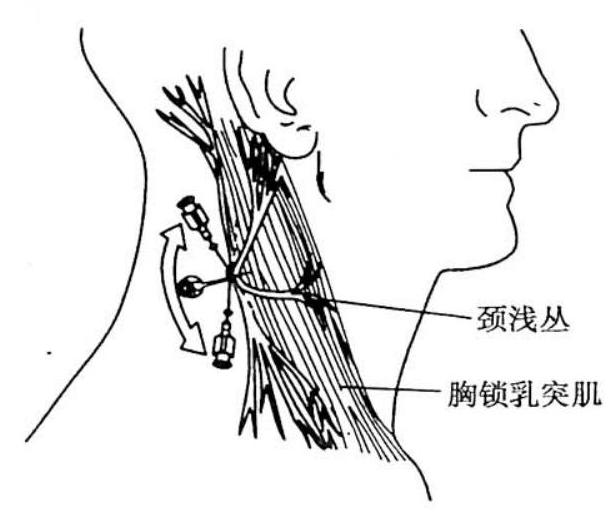
\includegraphics[max width=\textwidth]{2024_07_09_002a177993bd97d1d6d7g-052}
\end{center}

图 3-2 颈浅丛解剖及阻滞方法阻滞。注药时压迫远端或将患者置于头低位有助于局麻药向上扩散。

\section*{(四)颈神经丛阻滞的并发症}
并发症多见于颈深丛阻滞, 发生率较低, 常见并发症有: (1)局麻药毒性反应: 多由穿刺针误人血管所致, 因此每次注药前应回吸; (2)喉返神经阻滞: 可导致患者声音嘶哑或失声, 尤以双侧阻滞时较易发生; (3)膈神经阻滞: 常易累及膈神经, 双侧受累时可出现呼吸困难及胸闷, 应谨慎进行双侧颈深丛阻滞; (4)霍纳综合征: 由于颈交感神经被阻滞,而出现同侧眼睑下垂、瞳孔缩小、球结膜充血、鼻塞、面微红等症状; (5)高位硬膜外阻滞或全脊麻: 主要由于穿刺针进入硬脊膜外隙或蛛网膜下隙而引起。

\section*{三. 譬神经从阴篮}
\section*{(一)解剖}
臂神经丛由颈 ${ }_{5-8}\left(\mathrm{C}_{5} \sim \mathrm{C}_{8}\right)$ 及胸 $丨_{1}\left(\mathrm{~T}_{1}\right)$ 脊神经前支组成, 有时也接受颈 ${ }_{4}\left(\mathrm{C}_{4}\right)$ 及胸 $)_{2}\left(\mathrm{~T}_{2}\right)$ 脊神经前支发出的小分支, 主要支配整个手、臂运动和绝大部分感觉(图 3-3)。组成臂丛的脊神经出椎间孔后在锁骨上部,肌间沟内分为上、中、下三干。上干由 $\mathrm{C}_{5} \sim \mathrm{C}_{6}$ 前支, 中干由 $\mathrm{C}_{7}$ 前支,下干由 $\mathrm{C}_{8}$ 和 $\mathrm{T}_{1}$ 、 $\mathrm{T}_{2}$ 脊神经前支构成。三支神经干穿出肌间沟后,在锁骨下动脉的后上方沿第 1 肋骨上缘穿行。至锁骨后第 1 肋骨的外缘,每个神经干又分为前、后两股,在锁骨中段后方进人腋窝。各股神经在腋窝重新组合成三束,三个后股在腋动脉后方合成后束, 延续为腋神经及桡神经; 上干和中干的前股在腋动脉的外侧合成外侧束, 延续为肌皮神经和正中神经外侧头; 下干的前股延伸为内侧束, 延续为尺神经、前臂内侧皮神经、臂内侧皮神经和正中神经内侧头。覆盖前、中斜角肌的椎前筋膜向外融合包裹臂神经丛形成筋膜鞘,此鞘从椎间孔延伸至上臂上部, 是臂神经丛阻滞的解剖基础。

\section*{(二)局麻药的选择}
臂神经从阻滞药物需要较大容量 (20~40ml)以利于药物在鞘内扩散,而浓度不必太高。可

\begin{center}
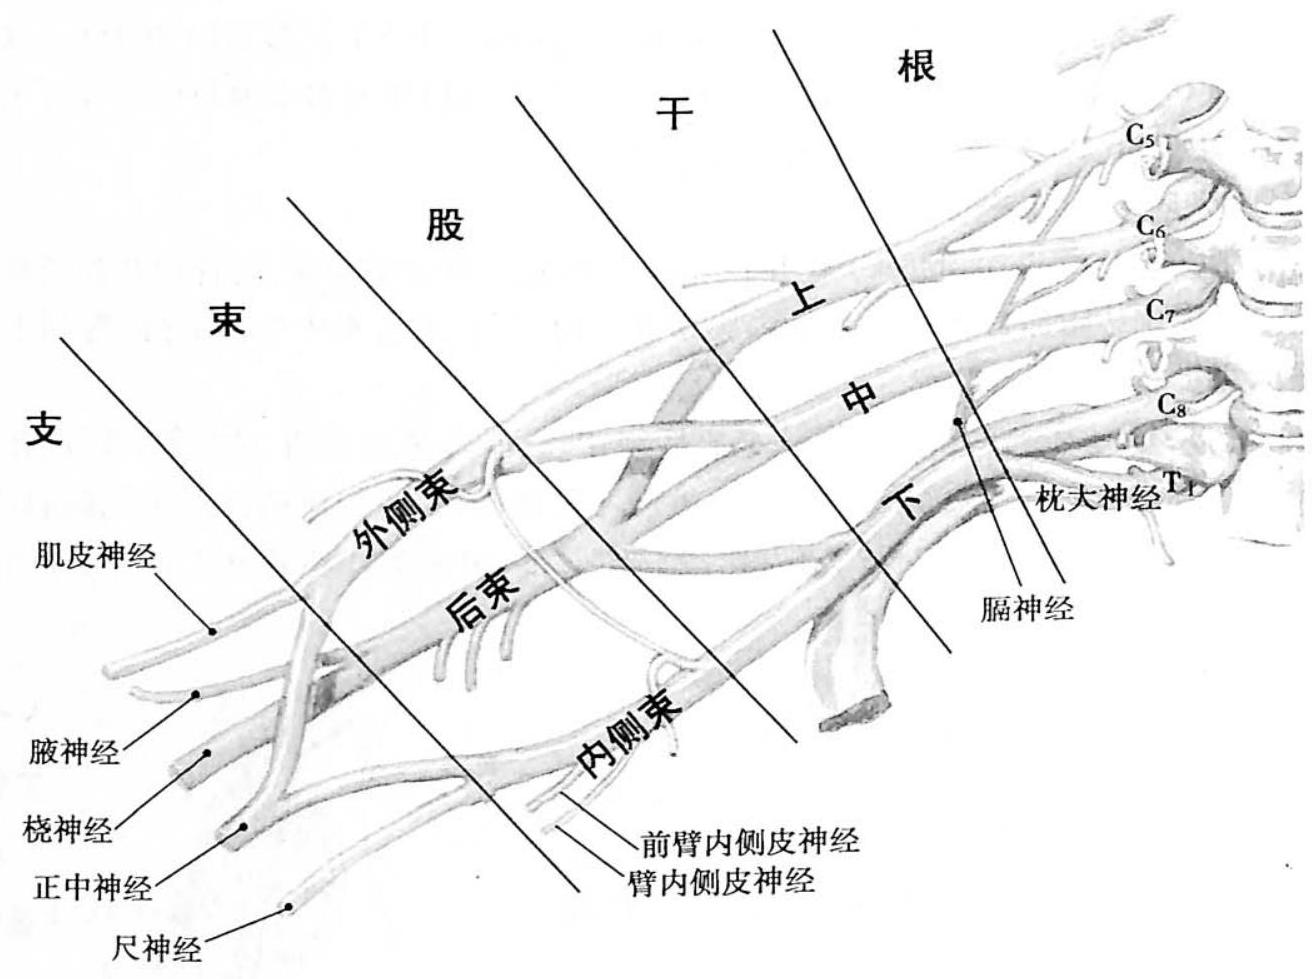
\includegraphics[max width=\textwidth]{2024_07_09_002a177993bd97d1d6d7g-053}
\end{center}

图 3-3 臂神经丛解剖示意图

选用一种局麻药或两种局麻药的混合液。2 4 小时的手术可选用 1\% 1.5\% 利多卡因; 若手术时间较长, 可选用 $0.25 \% \sim 0.5 \%$ 的布比卡因或罗哌卡因。

\section*{(三)操作方法和临床应用}
从包裹臂神经丛筋膜鞘的任何位置注人局麻药均可扩散并阻滞 $\mathrm{C}_{5} \sim \mathrm{T}_{1}$ 神经根, 但神经阻滞的程度随注射部位的变化而不同。临床上常根据手术需要选择不同途径进行臂神经丛阻滞 (brachial plexus block)。常用阻滞途径为肌间沟、腋窝和锁骨上人路。

\begin{enumerate}
  \item 肌间沟入路法 (interscalene block)
\end{enumerate}

(1)适应证: 适用于肩部、上臂和前臂手术。在肌间沟水平注人局麻药, $\mathrm{C}_{5} \sim \mathrm{C}_{7}$ 皮区的阻滞效果最强, 而 $\mathrm{C}_{8} \sim \mathrm{T}$, 皮区的阻滞效果较弱。因此, 肌间沟人路臂丛阻滞不能为尺神经分布区的手术提供良好的麻醉效果。

(2)操作方法: 肌间沟为前、中斜角肌与肩胛舌骨肌共同构成的一个三角区。患者去枕平卧, 头偏向对侧, 手臂贴体旁 (图 3-4)。在胸锁乳突肌锁骨端外缘触及前斜角肌, 再向后外侧滑过前斜角肌肌腹即为前、中斜角肌之间的肌间沟。从环状软骨向后作一水平线,与肌间沟的交点即为穿刺点。皮肤常规消毒后, 用 $22 \sim 25 \mathrm{G}$ 穿刺针垂直刺人皮肤, 略偏向内侧和尾侧方向进针, 同时观察异感或电刺激诱发浅层肌肉收缩反应, 以手臂或肩部出现异感或电刺激引发肌肉收缩为准确定位的标志。准确定位后将针头固定, 回吸无异常可注人局麻药 $20 \sim 30 \mathrm{ml}$ 。一般情况下, 肌间沟人路很难阻滞尺神经,将患者置于头高位并压迫穿刺点上方有助于局麻药向下扩散, 从而阻滞尺神经。

(3) 优缺点

1)优点:(1)易于掌握;(2)上臂、肩部及桡侧阻滞效果好; (3)不易引起气胸。

\begin{enumerate}
  \setcounter{enumi}{1}
  \item 缺点:(1)尺神经阻滞起效慢; (2) 有误人蛛网膜下隙或硬脊膜外弥的危险; (3)有损伤椎动脉的危险; (4)不宜
\end{enumerate}

\begin{center}
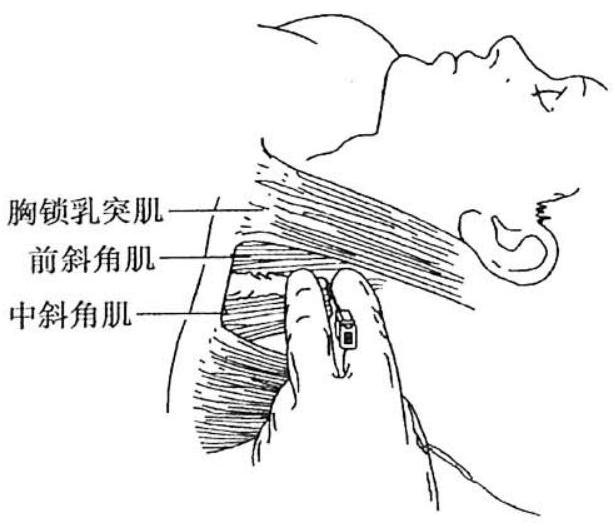
\includegraphics[max width=\textwidth]{2024_07_09_002a177993bd97d1d6d7g-053(1)}
\end{center}

图 3-4 肌间沟入路臂神经丛阻滞\\
同时双侧阻滞, 以免阻滞双侧膈神经或喉返神经。

\begin{enumerate}
  \setcounter{enumi}{1}
  \item 锁骨上入路法(supraclavicular block)
\end{enumerate}

(1)适应证:由于臂神经丛三条主干都集中在锁骨上、第 1 肋骨正上方,因此,通过锁骨上人路阻滞臂神经丛适用于上臂、前臂和手部手术。

(2)操作方法:患者去枕平卧,头转向对侧,上肢紧贴体旁(图 3-5)。穿刺点位于肌间沟最低点, 锁骨下动脉搏动处后上方, 此处位于锁骨中点上方 $1 \sim 1.5 \mathrm{~cm}$ 。以 $22 \mathrm{G}$ 穿刺针向尾侧刺入皮肤,直至引出异感或电刺激引发肌肉收缩反应时,将针头固定, 回吸无异常后注人局麻药 20~ $30 \mathrm{ml}$ 。如针尖碰到第 1 肋骨仍未引出异感,可将穿刺针稍许后退再沿肋骨面向前或向后穿刺,直至引出异感。

(3)优缺点

1)优点: (1)用较小药量可得到较满意的阻滞效果;(2)穿刺中不需移动上肢, 对上肢外伤疼痛者较适合; (3)不易发生误人硬脊膜外隙或蛛网膜下隙的危险。

2)缺点:(1)气胸发生率较高 ( $0.5 \% \sim 6 \%)$, 而且气胸症状可延迟出现; (2)星状神经节及膈神经阻滞的发生率较高。

\section*{3. 腋入路法 ( axillary block)}
(1)适应证: 腋动脉是腋人路阻滞时最重要的定位标志。正中神经位于腋动脉的上方, 尺神经位于其下方,而桡神经位于其后外侧。肌皮神经在腋

\begin{center}
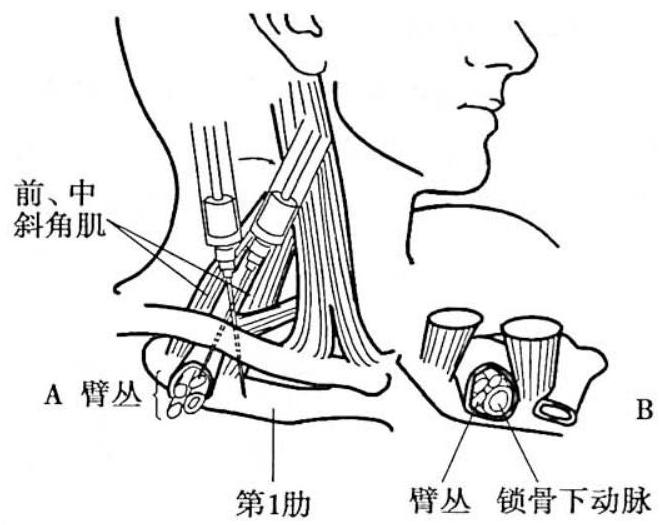
\includegraphics[max width=\textwidth]{2024_07_09_002a177993bd97d1d6d7g-054(1)}
\end{center}

图 3-5 锁骨上入路臂神经丛阻滞

A. 锁骨上人路臂神经丛阻滞方法;

B. 臂神经丛在第 1 肋水平排列窝已经离开了血管神经鞘,进人啄肱肌; 来自 $\mathrm{T}_{2}$ 肋间神经分支的肋间臂神经位于腋动脉的表面。因此, 腋人路臂神经丛阻滞适用于肘部至手部手术, 在 $\mathrm{C}_{7} \sim \mathrm{T}_{1}$ ( 尺神经) 皮区的阻滞效果最强, 但对肩部和上臂 $\left(\mathrm{C}_{5} \sim \mathrm{C}_{6}\right)$ 手术的阻滞效果稍差;同时也难以阻滞肌皮神经, 但可以在腋部或肘部补救。

\begin{center}
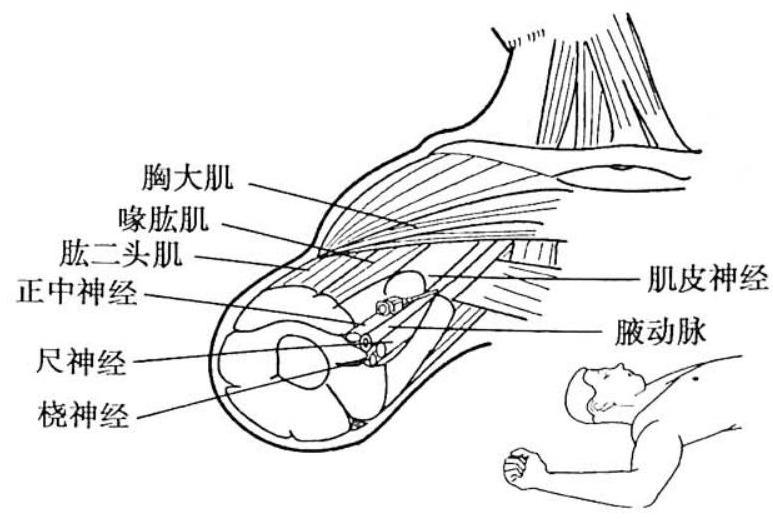
\includegraphics[max width=\textwidth]{2024_07_09_002a177993bd97d1d6d7g-054}
\end{center}

图 3-6 腋入路臂神经丛阻滞

(2)操作方法: 患者平卧,头偏向对侧,被阻滞的上臂外展与躯干成直角, 肘关节屈曲 $90^{\circ}$, 肩部外旋上臂横过头顶, 似行军礼状以充分显露腋窝。先在腋窝触摸腋动脉搏动,再沿腋动脉上行摸到胸大肌下缘动脉搏动最强处即为穿刺点 (图 3-6)。以穿刺针在动脉边缘刺人皮肤, 然后缓慢进针直到出现刺破鞘膜的落空感,或同时出现异感; 松开持针手指, 针头可随动脉搏动而摆动, 即可认为针已进人腋鞘内; 接注射器回抽无血后注人局麻药 $25 \sim 35 \mathrm{ml}$ 。腋人路阻滞一般无需寻找异感, 只要穿刺针进人血管神经鞘内均可获得良好的阻滞效果, 多点注射可提高阻滞效果。经腋人路阻滞时, 肌皮神经和肋间臂神经常不能被完善阻滞, 肌皮神经阻滞是完善的前臂和腕部麻醉的基础, 而肋间臂神经成功阻滞可避免应用止血带部位疼痛。故在注药完毕后, 改变穿刺针方向, 使针头位于腋动脉上方并与皮肤垂直进针, 刺人啄肱肌进行扇形封闭; 然后将针退至皮下,在腋动脉下方腋窝下缘注药以阻滞肋间臂神经, 可获得良好效果。

(3)优缺点

1)优点:(1)位置表浅,动脉搏动明显,易于阻滞; (2)不会引起气胸; (3)不会阻滞膈神经、迷走\\
神经、喉返神经; (4)无误人硬脊膜外隙或蛛网膜下隙的危险; (5)可放人留置针或导管行连续阻滞。

\begin{enumerate}
  \setcounter{enumi}{1}
  \item 缺点:(1)上肢不能外展或腋窝部位有感染、肿瘤的患者不能应用; (2)因局麻药用量较大,局麻药毒性反应发生率较其他方法高。
\end{enumerate}

\section*{四、下肢神经阻滞}
腰麻和硬膜外阻滞是下肢手术最常用的区域麻醉方法, 而下肢神经阻滞不仅可为下肢手术提供良好的麻醉, 而且因不阻滞交感神经, 避免了因血管扩张导致的血压下降, 对某些重症患者具有重要意义。

\section*{(一)解剖}
支配下肢的神经来自于腰丛和骶丛神经。腰丛由腰,$_{1} \sim$ 腰 $_{4}\left(\mathrm{~L}_{1} \sim \mathrm{L}_{4}\right)$ 前支构成, 常有胸 ${ }_{12}$ $\left(\mathrm{T}_{12}\right)$, 偶有腰 $\left(\mathrm{L}_{5}\right)$ 分支参与。由 $\mathrm{L}_{2} \sim \mathrm{L}_{4}$ 组成的腰丛成分主要支配大腿的前、内侧; $\mathrm{L}_{2} \sim \mathrm{L}_{4}$ 的前支组成闭孔神经, 后支组成股神经, 而 $\mathrm{L}_{2}$ 和 $\mathrm{L}_{3}$ 的后支又组成股外侧皮神经 (图 3-7)。腰丛神经位于腰大肌和腰方肌之间的腰大肌间隙内。

\begin{center}
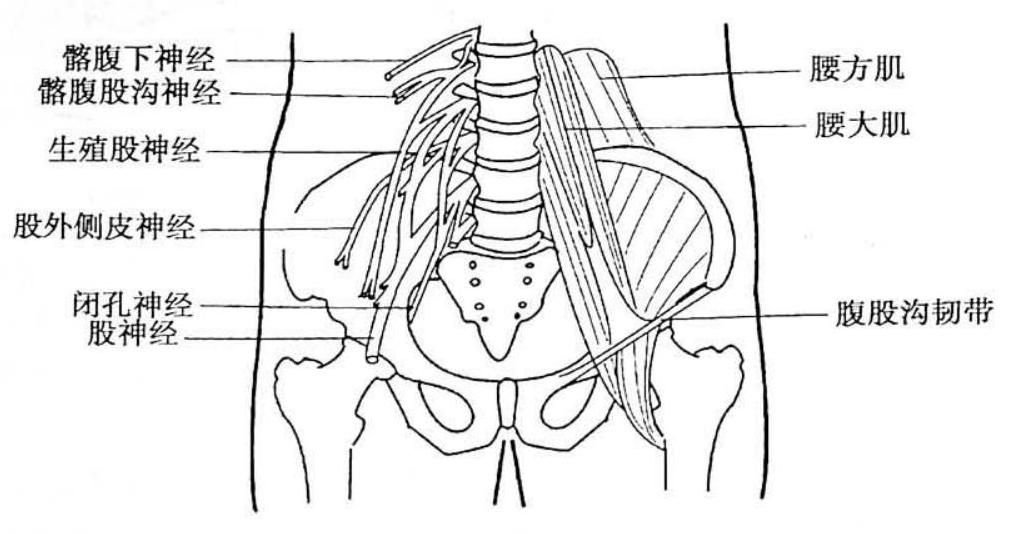
\includegraphics[max width=\textwidth]{2024_07_09_002a177993bd97d1d6d7g-055}
\end{center}

图 3-7 腰神经丛解剖图

髊丛来源于骶 $\sim$ 骶 $\left(\mathrm{S}_{1} \sim \mathrm{S}_{3}\right)$ 骬神经和 $\mathrm{L}_{4}$ 和 $\mathrm{L}_{5}$ 前支的分支, 主要构成股后皮神经和坐骨神经, 一起经过坐骨大孔穿出骨盆, 支配下肢后面和足的运动和感觉。坐骨神经包含胫神经和腓总神经的主于 (由 $\mathrm{L}_{4} 、 \mathrm{~L}_{5} 、 \mathrm{~S}_{1} \sim \mathrm{S}_{3}$ 前支的腹侧支组成胫神经, 背侧支组成腓总神经), 二者在腘窝或腘窝上方从坐骨神经分出后, 胫神经走行在内侧而腓总神经绕到外侧下行。

\section*{(二)腰神经丛阻滞(腰肌间祘阻滞) ( lumbar plexus block)}
\begin{enumerate}
  \item 适应证 腰神经丛阻滞可同时阻滞股外侧皮神经、股神经和闭孔神经。因此,适用于膝部、大腿前部和䯘部手术; 加上坐骨神经阻滞可阻滞整个下肢; 置人导管可用于滕关节和骹关节的术后持续镇痛。

  \item 操作方法一般采用后路法。患者侧卧位, 患肢置于上部。确认双侧骼塍并作一连线,此线常通过第 4 腰椎。在患侧连线上、由脊柱旁开 $5 \mathrm{~cm}$ 处即为穿刺点。穿刺针由穿刺点垂直进针, 直达第 4 腰椎横突; 然后针尖向尾侧滑过第 4 腰椎横突下缘; 继续进针约 $0.5 \mathrm{~cm}$ 后有明显落空感, 表明针已进人腰大肌间隙内; 回吸无异常后注人局麻药 $20 \sim 30 \mathrm{ml}$ (图 3-8)。用神经刺激器定位, 当电流小于 $0.5 \mathrm{~mA}$ 时仍有股四头肌收缩反应, 可确定穿刺针已抵达腰丛。

  \item 并发症 后路法腰丛阻滞进针过深时, 有进人硬脊膜外隙、蛛网膜下隙或血管内的危险;也有导致血肿和神经损伤的可能。

\end{enumerate}

\section*{(三)股神经阻滞(三合一阻滞)(the femoral 3 in 1 block)}
\begin{enumerate}
  \item 适应证 股神经主要支配大腿前部肌肉(股四头肌、缝匠肌和耻骨肌)以及从腹股沟韧带到膝部的皮肤。股神经阻滞可用于大腿前部和膝关节手术,常与其他下肢阻滞技术联合
\end{enumerate}

\begin{center}
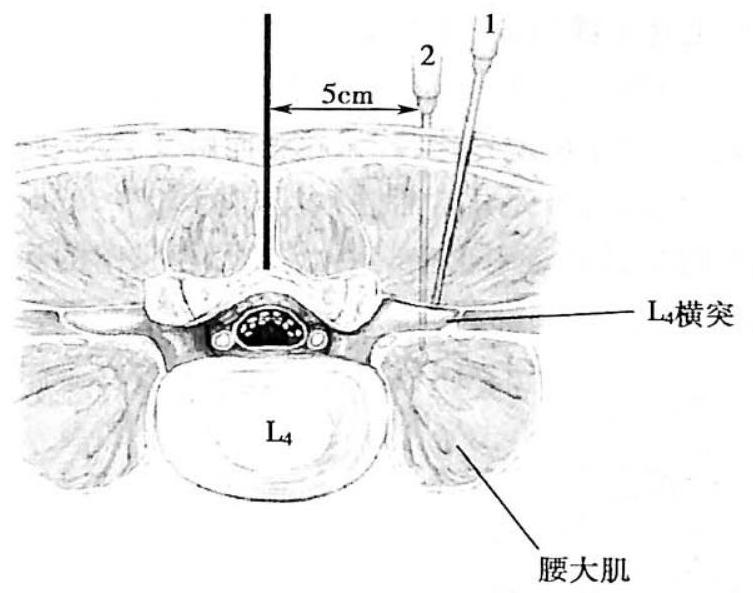
\includegraphics[max width=\textwidth]{2024_07_09_002a177993bd97d1d6d7g-056(2)}
\end{center}

A

\begin{center}
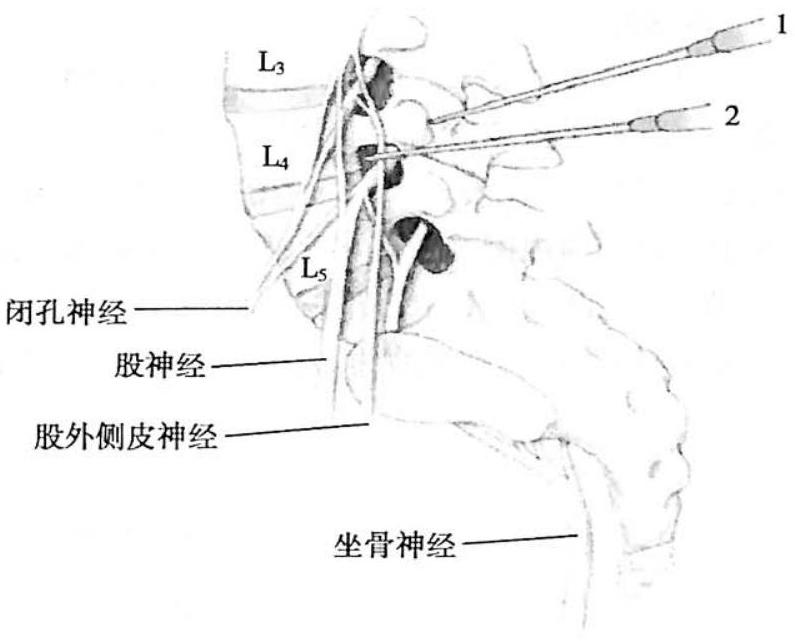
\includegraphics[max width=\textwidth]{2024_07_09_002a177993bd97d1d6d7g-056(1)}
\end{center}

B

图 3-8 腰神经丛阻滞

如图 A 所示,穿刺针先达第 4 腰椎横突 (针 1), 然后针尖向尾侧滑过第 4 腰椎横突下缘 (针 2), 进人腰大肌间隙

应用。

\begin{enumerate}
  \setcounter{enumi}{1}
  \item 操作方法 患者仰卧位,在腹股沟韧带中点可扪及股动脉搏动,穿刺点即在腹股沟韧带下方, 股动脉搏动点外侧。将穿刺针与皮肤呈 $45^{\circ}$ 向头侧方向进针,出现异感则表明位置正确,回抽无异常后注人局麻药 $20 \sim 30 \mathrm{ml}$ 。使用神经刺激仪定位时, 通常先找到股神经前支,表现为大腿内侧缝匠肌收缩, 此时应将针尖稍向外侧重新进针,抵达股神经后支时可引发股四头肌收缩, 回抽无异常后注人局麻药(图 3-9)。注药时同时压迫股管远端, 使局麻药向近端扩散进人腰肌间隙,不仅可阻滞股神经,而且可阻滞闭孔神经和股外侧皮神经, 因此也称为 “三合一阻滞”。但此方法对闭孔神经阻滞常不完善,故一般仅将其视为单纯股神经阻滞。
\end{enumerate}

\begin{center}
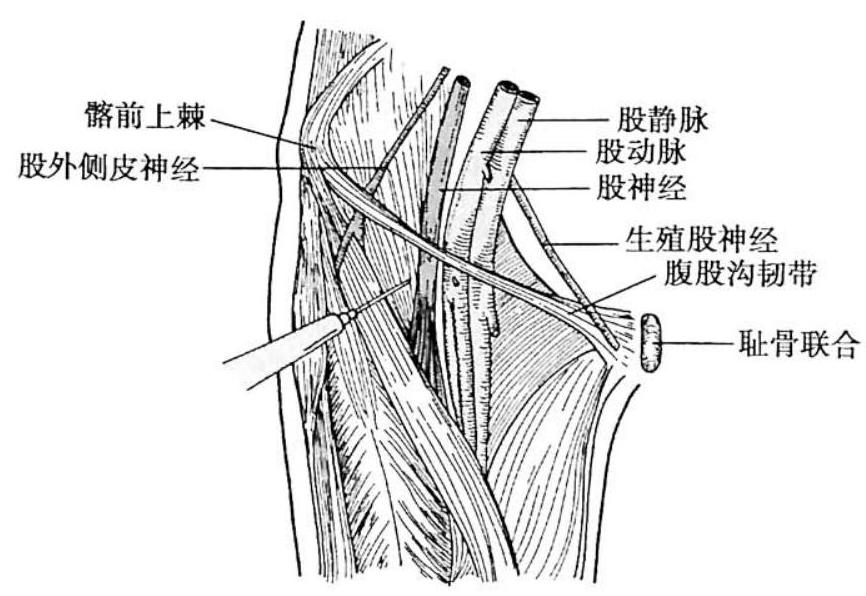
\includegraphics[max width=\textwidth]{2024_07_09_002a177993bd97d1d6d7g-056}
\end{center}

图 3-9 股神经阻滞

\begin{enumerate}
  \setcounter{enumi}{2}
  \item 并发症 由于穿刺点接近动脉,因此容易误伤动脉或将局麻药注人血管内。
\end{enumerate}

\section*{(四)坐骨神经阻滞(sciatic nerve block)}
\begin{enumerate}
  \item 适应证 坐骨神经主要支配迌肌和膝盖远端所有下肢肌肉的运动, 以及除隐神经支配的内侧面外,膝部远端下肢的所有感觉。临床上可联合隐神经或股神经阻滞用于膝关节以下无需止血带的手术。股后皮神经前段与坐骨神经伴行, 支配大腿后部的皮肤,坐骨神经阻滞的同时也阻滞该神经。
\end{enumerate}

\section*{第三章 局 部 麻 醉}
\section*{2. 操作方法}
(1)经典后路法: 患者取侧卧位, 阻滞侧下肢在上并屈髋屈膝, 膝关节呈 $90^{\circ}$ 角, 健侧下肢伸直。由股骨大转子与髂后上棘作一连线, 连线中点作一条垂直线, 与股骨大转子与骶裂孔连线的交点即穿刺点(图 3-10)。使用 $22 \mathrm{G}$ 穿刺针垂直进针, 直至出现异感, 若无异感而触及骨质, 则针尖可略偏向内侧或外侧再穿刺。出现异感后针稍后退, 回吸无异常后注人局麻药 $20 \sim 30 \mathrm{ml}$ 。使用神经刺激仪时, 在出现臀肌刺激反应后, 继续向前进针直至引出坐骨神经支配区肌肉的运动反应(腘肌或腓肠肌收缩、足屈或趾屈),回吸无异常后注人局麻药。

\begin{center}
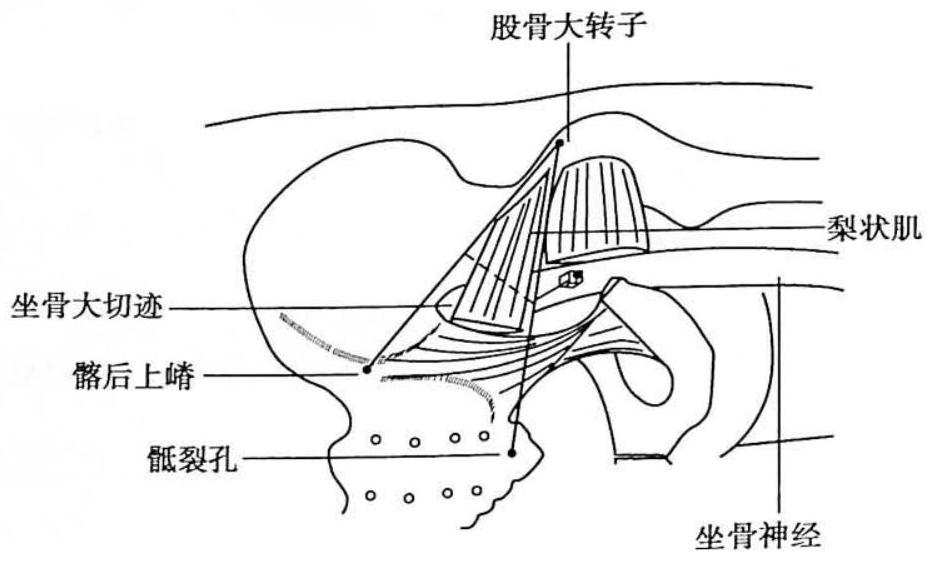
\includegraphics[max width=\textwidth]{2024_07_09_002a177993bd97d1d6d7g-057}
\end{center}

图 3-10 后路法坐骨神经阻滞

(2)前路法:患者仰卧,从大转子作一条平行于腹股沟韧带的直线,再沿腹股沟韧带将髂前上棘到耻骨结节连线分为三等分, 在中、内 $1 / 3$ 处作一垂直线与上述大转子线相交, 交点即为穿刺点。将穿刺针垂直进针后稍偏向外侧, 遇到骨质即为股骨小转子。将针尖向内侧滑过股骨并继续进针 $5 \mathrm{~cm}$ 左右可引出异感,使用神经刺激仪时可出现肌肉收缩反应, 回吸无异常后注人局麻药。该方法穿刺部位较深,操作较为困难。

\begin{enumerate}
  \setcounter{enumi}{2}
  \item 并发症 常见并发症为阻滞不全和神经损伤。
\end{enumerate}

\section*{第四章椎管内麻醉}
椎管内麻醉 (intrathecal anesthesia)包括蛛网膜下弥阻滞[ 简称腰麻 (spinal anesthesia) ] 和硬脊膜外弥阻滞 (epidural anesthesia)(含骶管阻滞)。将局麻药注人蛛网膜下隙, 暂时使脊神经前根和后根的神经传导阻滞的麻醉方法称为蛛网膜下弥阻滞; 将局麻药注人硬脊膜外陌, 暂时阻断脊神经根的神经传导的方法, 称为硬脊膜外隙阻滞, 简称硬膜外阻滞。蛛网膜下弥阻滞的特点为所需麻醉药的剂量和容量较小, 但能使感觉和运动神经阻滞完善, 麻醉效果确切。而硬膜外阻滞则需要局麻药的剂量和容量均较大,药物吸收进人血液循环可能导致全身副作用; 其优点是可以通过置管而连续给药, 有利于时间长短不能确定的手术。蛛网膜下陌-硬膜外联合阻滞 (combined spinal-epidural anesthesia, CSEA) 则可取两者的优点, 在临床麻醉中应用日趋广泛。

椎管内麻醉能有效阻断外科手术刺激对机体产生的应激反应 (stress response)、减少术中出血量、降低术后血检的发生; 应用这些技术能缩短患者的住院时间, 从而更加有效地利用卫生保健经费。

\section*{第一节 椎管内解剖与麻醉生理}
\section*{一、椎管解剖}
\section*{(一) 脊椎的结构}
脊椎由 7 节颈椎、12 节胸椎、5节腰椎、融合成一块的 5 节骶椎及 $3 \sim 4$ 节尾椎组成。成人脊椎有 4 个弯曲, 颈曲和腰曲向前, 胸曲和骶曲向后。仰卧位时, 脊椎的最高点位于第 3 腰椎和第 3 颈椎, 最低点位于第 5 胸椎和骶部(图 4-1)。脊椎由椎体、椎弓及棘突组成, 相邻两个上下椎弓切迹之间构成椎间孔, 脊神经根由此通过。颈椎与腰椎的棘突呈水平状排列, 胸椎棘突呈叠瓦状排列。每个椎体与后方呈半环形的椎弓共同构成椎孔, 所有椎孔连通呈管状, 称为椎管。椎管上起枕骨大孔,下止于骶裂孔;在骶椎部分的椎管称为骶管。

\begin{center}
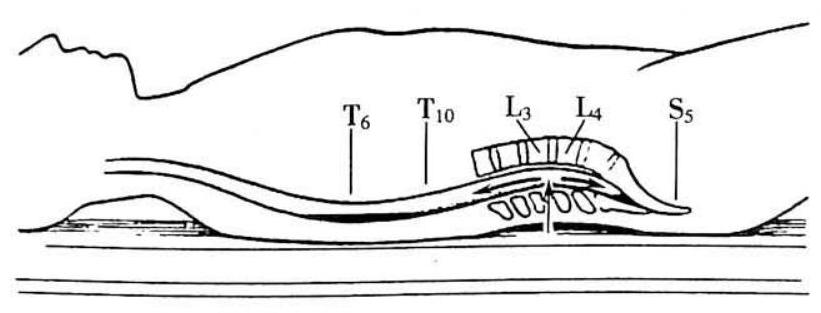
\includegraphics[max width=\textwidth]{2024_07_09_002a177993bd97d1d6d7g-058}
\end{center}

图 4-1 脊柱的生理弯曲示意图

\section*{(二)韧带}
相邻两个椎骨的椎弓板由 3 条韧带相互连接, 从内向外的顺序为: 黄韧带、棘间韧带和棘上韧带( 图 4-2)。黄韧带位于相邻椎弓板之间, 由黄色的弹力纤维构成, 坚韧并富有弹性, 从上位椎板内面的下缘连至下位椎板外面的上缘, 参与构成椎管的后壁和后外侧壁。黄韧带的宽度约为椎管后壁的 $1 / 2$, 腰部最为坚韧厚实, 穿刺时可借助穿刺针触及该韧带有坚韧和阻力感, 而再向前进针, 一旦阻力消失, 便知进人硬脊膜外隙。棘间韧带位于棘突之间, 较薄弱; 而棘上韧带为连接各棘突尖的纵行軔带,老年人棘上韧带可钙化。

\section*{第四章椎管内麻醉}
\begin{center}
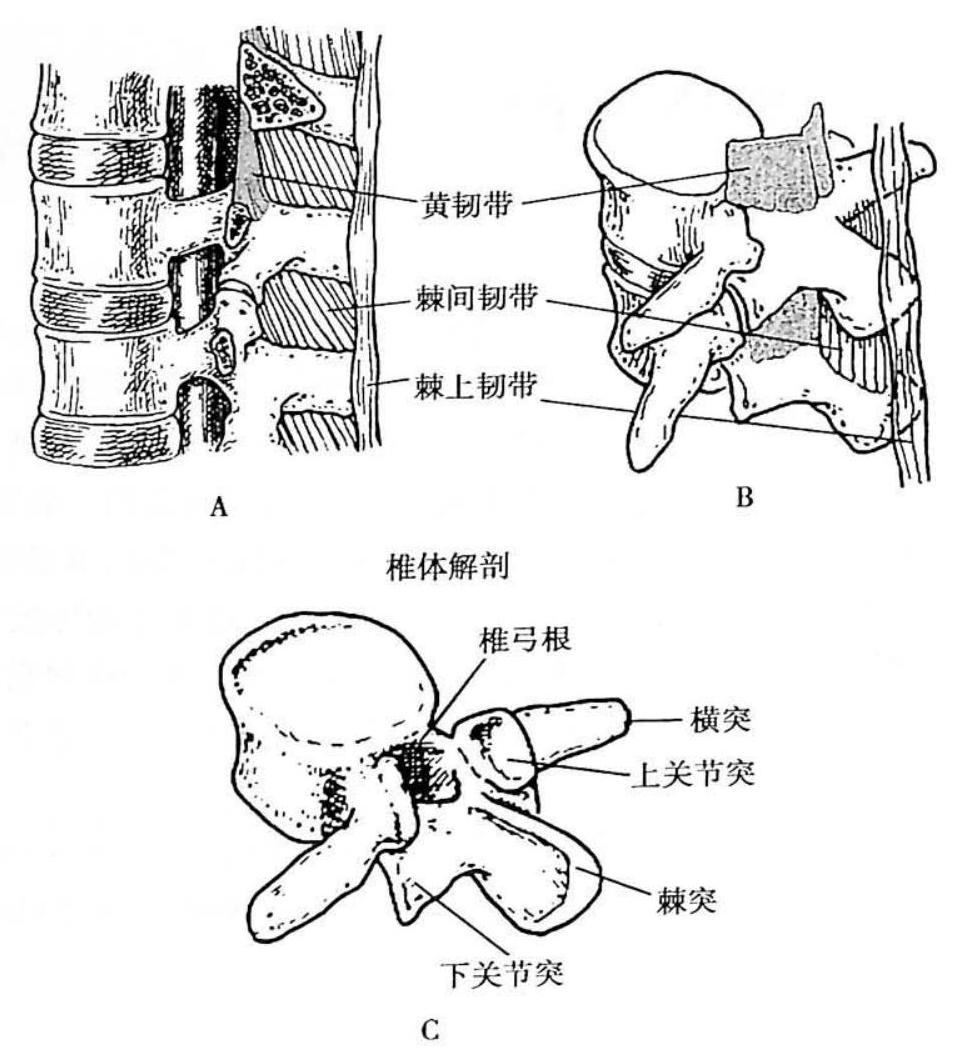
\includegraphics[max width=\textwidth]{2024_07_09_002a177993bd97d1d6d7g-059}
\end{center}

图 4-2 腰椎解剖示意图

A. 矢状图;B. 腰椎骨斜位图;C. 单个腰椎骨斜位图

\section*{(三)脊髓}
脊髓位于椎管内, 上端从枕骨大孔开始, 在胚胎期充满整个椎管腔, 新生儿终止于第 3 或第 4 腰椎, 成人则终止于第 1,2 腰椎之间。在成人第 2 腰椎以下、小儿第 3 腰椎以下的蛛网膜下隙只有脊神经根, 即马尾神经。所以, 蛛网膜下皕穿刺时, 成人应在第 2 腰椎以下、小儿应在第 3 腰椎以下的间隙穿刺,以免损伤脊髓(图 4-3)。

\section*{(四)脊膜与腔隙}
脊髓有三层被膜,即软脊膜、蛛网膜和硬脊膜。软脊膜紧贴于脊髓表面,与蛛网膜之间形成的腔隙为蛛网膜下隙。蛛网膜下弥除有脊髓外, 还充满脑脊液。成人脑脊液总量约 $120 ~$ $150 \mathrm{ml}$, 其中蛛网膜下临含有 $25 \sim 30 \mathrm{ml}$ 。正常脑脊液无色透明, $\mathrm{pH} 7.35$, 比重 $1.003 \sim 1.009$; 压力平卧位时约 $100 \mathrm{mmH}_{2} \mathrm{O}$, 侧卧位时 $70 \sim 170 \mathrm{mmH}_{2} \mathrm{O}$, 坐位时 $200 \sim 300 \mathrm{mmH}_{2} \mathrm{O}$ 。蛛网膜与硬脊膜之间形成的潜在腚隙为硬脊膜下隙, 此间隙在颈部较宽, 在行颈部硬脊膜外隙阻滞或颈从、肌间沟臂丛阻滞时容易误人此间隙。硬脊膜与椎管内壁 (即黄韧带) 之间构成硬脊膜外隙, 其内充满血管、脂肪、淋巴及疏松结缔组织。成人硬脊膜外隙容积约 $100 \mathrm{ml}$, 其中骶管约 $25 \sim 30 \mathrm{ml}$ 。在奼娠晚期, 硬脊膜外隙的静脉丛呈怒张状态, 老年人由于骨质增生及纤维化使椎管变窄, 均可使硬脊膜外隙变小。

硬脊膜、蛛网膜和软脊膜均可沿脊神经根向两侧延伸, 并包裹脊神经根, 分别称为根硬脊膜、根蛛网膜和根软脊膜。根硬脊膜随着向椎间孔延伸而逐渐变薄。根蛛网膜细胞增生可形成线

\begin{center}
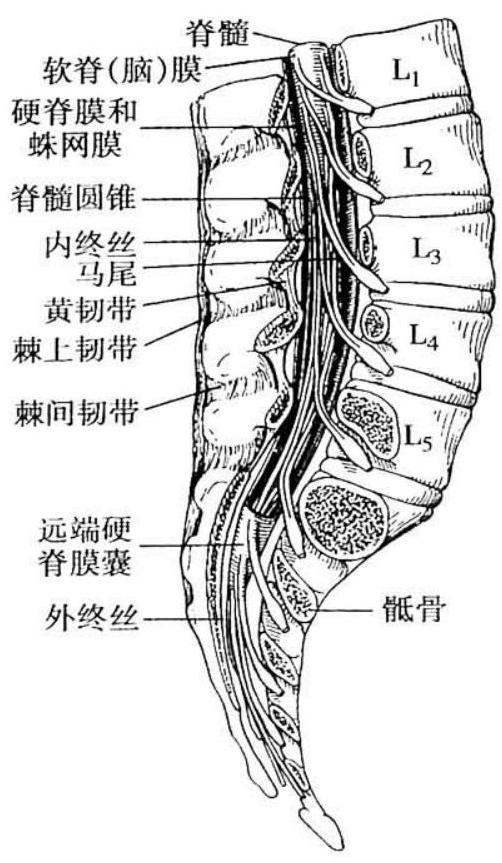
\includegraphics[max width=\textwidth]{2024_07_09_002a177993bd97d1d6d7g-059(1)}
\end{center}

图 4-3 腰骶部脊髓解剖示意图\\
毛结构,并可突进或穿透根硬脊膜。根蛛网膜和根软脊膜之间的腔隙称根蛛网膜下隙, 与脊髓部蛛网膜下隙相通,在椎间孔处闭合成盲淬。在蛛网膜下隙注人墨汁时,可见墨水颗粒聚积在根蛛网膜下隙处, 故又称墨水套襄。蛛网膜线毛有利于引流脑脊液和清除蛛网膜下隙的颗粒物。

\section*{(五)骶管}
骶管是硬脊膜外隙的一部分,呈三角形。骶管上自硬脊膜虂,即第 2 骶椎水平,终止于骶裂孔。行骶管穿刺时,切勿超过第 2 骶椎水平, 以免误人蛛网膜下隙。

\section*{(六)脊神经及体表标志}
脊神经共 31 对,包括 8 对颈神经、 12 对胸神经、 5 对腰神经、 5 对骶神经和 1 对尾神经。每对脊神经分为前根和后根, 前根从脊髓前角发出,由运动纤维和交感神经传出纤维组成;后根由感觉纤维和交感神经传人纤维组成。脊神经在人体皮肤分布的体表标志为: 甲状软骨部位为 $\mathrm{C}_{2}$, 胸骨上缘为 $\mathrm{T}_{2}$, 双乳头连线为 $\mathrm{T}_{4}$, 剑突下为 $\mathrm{T}_{6}$, 平脐为 $\mathrm{T}_{10}$, 耻骨联合水平为 $\mathrm{T}_{12}$ ( 图 4-4)。

\begin{center}
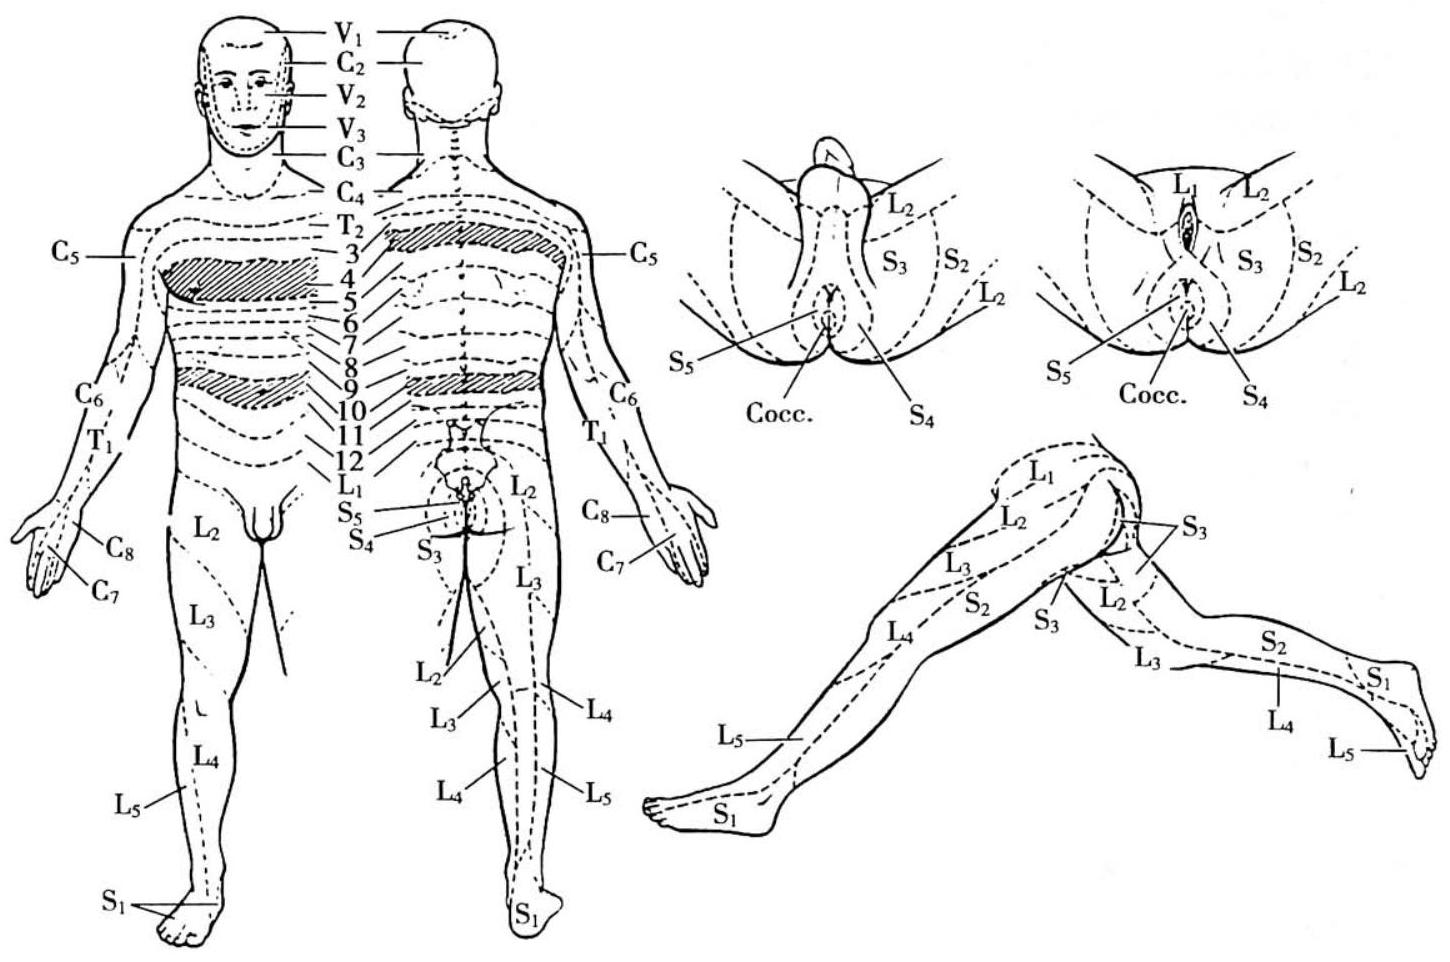
\includegraphics[max width=\textwidth]{2024_07_09_002a177993bd97d1d6d7g-060}
\end{center}

图 4-4 脊神经体表分布示意图

$\mathrm{C}=$ 颈 $; \mathrm{T}=$ 胸 $; \mathrm{L}=$ 腰 $; \mathrm{S}=$ 骶; $\mathrm{Cocc}=$ 尾

\section*{二、椎管内阻滞的生理}
\begin{enumerate}
  \item 椎管内麻醉药物作用部位 目前认为,椎管内麻醉药物作用的主要部位是脊神经。蛛网膜下隙阻滞时, 局麻药经脑脊液稀释和扩散后直接作用于脊神经根和脊髓表面, 但主要是作用于脊神经根。硬膜外阻滞的机制比较复杂,多数意见为:11椎旁阻滞,药液由硬膜外间隙经椎间孔渗出,在椎旁阻滞脊神经根; (2)通过蛛网膜线毛进人根蛛网膜下隙,作用于脊神经根; (3)直接透过硬脊膜和蛛网膜进入蛛网膜下隙,作用于脊神经根和脊髓表面。

  \item 阻滞顺序由于传递冲动的神经纤维互不相同, 局麻药的阻滞顺序为, 自主神经纤维先被阻滞,感觉神经纤维次之,运动神经纤维及有髓鞘的本体感觉纤维 ( $\mathrm{A}_{\gamma}$ 纤维 $)$ 最后被阻滞。不同神经纤维被阻滞顺序依次为: 血管舒缩 $\rightarrow$ 冷感 $\rightarrow$ 温感 $\rightarrow$ 对不同温度的辨别 $\rightarrow$ 慢痛 $\rightarrow$ 快痛 $\rightarrow$ 触觉 $\rightarrow$ 运动 $\rightarrow$ 压力感 $\rightarrow$ 本体感。消退顺序与阻滞顺序相反。

\end{enumerate}

\section*{第四章 椎管内麻醉}
\begin{enumerate}
  \setcounter{enumi}{2}
  \item 阻滞平面差异 交感神经阻滞平面与感觉神经阻滞平面不一致,一般交感神经阻滞平面比感觉消失平面要高 $2 \sim 4$ 个神经节段, 感觉消失平面又比运动神经阻滞平面要高 $1 \sim 4$ 个节段。
\end{enumerate}

\section*{第二节 蛛网膜下隙阻滞}
\section*{一、蛛网膜下隙阻滞的临床应用}
\section*{(一)适应证}
\begin{enumerate}
  \item 下腹及盆腔手术 如阑尾切除术、疝修补术、膀胱及前列腺手术、子宫及附件手术等。

  \item 肛门及会阴部手术 如痔切除术、肚瘘切除术等, 采用鞍区麻醉 (saddle anesthesia) 则更合理。

  \item 下肢手术 如下肢的骨折或脱臼复位术、截肢术等, 其止痛效果比硬膜外阻滞更完全, 并可避免止血带所致不适。

  \item 分娩镇痛。

\end{enumerate}

\section*{(二)禁忌证或相对禁忌证}
\begin{enumerate}
  \item 中枢神经系统疾病 脊髓或脊神经根病变, 脊髓的慢性或退行性病变, 楨内高压患者。

  \item 全身性严重感染以及穿刺部位有炎症或感染者。

  \item 休克患者。

  \item 腹内压明显增高者,如腹腔巨大肿瘤、大量腹水。

  \item 精神病、严重神经官能症以及小儿等不合作患者。

  \item 脊柱外伤或有明显腰背痛病史者, 以及脊柱严重畸形者。

\end{enumerate}

\section*{(三)麻醉前准备和麻醉前用药}
\begin{enumerate}
  \item 术前访视 术前访视患者应明确以下问题:
\end{enumerate}

(1)是否适宜进行腰麻,有无腰麻禁忌证。从手术部位和时间考虑,应用腰麻是否安全可靠,阻滞时间是否合适。

(2)确定拟用局麻药的种类、剂量、浓度和配制方法,以及患者体位和穿刺点。

\begin{enumerate}
  \setcounter{enumi}{1}
  \item 麻醉前用药 蛛网膜下弥阻滞的麻醉前用药量不宜过大, 应使患者保持清醒状态, 以利于调节阻滞平面。
\end{enumerate}

\section*{(四)常用局部麻醉药}
\begin{enumerate}
  \item 普鲁卡因 (procaine) 用于蛛网膜下隙阻滞的普鲁卡因为高纯度的白色晶体。成人用量 $100 \sim 150 \mathrm{mg}$ 。常用浓度为 $5 \%$, 麻醉起效时间为 $1 \sim 5$ 分钟, 麻醉维持时间为 $45 \sim 90$ 分钟, 适用于短小手术。常用 $5 \%$ 普鲁卡因重比重液配制方法为: 普鲁卡因 $150 \mathrm{mg}$ 溶解于脑脊液 $3 \mathrm{ml}$ 中。

  \item 丁卡因 (tetracaine) 成人常用剂量为 $8 \sim 15 \mathrm{mg}$, 常用浓度为 $0.3 \% \sim 0.5 \%$ 。临床上用 $1 \%$ 丁卡因 $1 \mathrm{ml}$, 加 $10 \%$ 葡萄糖及 $3 \%$ 麻黄碱各 $1 \mathrm{ml}$, 配成丁卡因重比重液的标准配方, 即所谓的 $1: 1: 1$ 溶液。起效时间为 $5 \sim 10$ 分钟, 20 分钟后阻滞平面固定, 麻醉维持时间为 $2 \sim 3$ 小时。

  \item 布比卡因 (bupivacaine) 为目前蛛网膜下隙阻滞的最常用药物, 成人常用剂量为 $8 \sim$ $15 \mathrm{mg}$ 。一般用 $0.5 \% \sim 0.75 \%$ 布比卡因 $2 \mathrm{ml}$, 加脑脊液 $1 \mathrm{ml}$, 配成重比重溶液, 麻醉维持时间为 $2 \sim 2.5$ 小时。布比卡因起效时间需 $5 \sim 10$ 分钟, 麻醉平面调节不可操之过急, 以免平面过高。

  \item 左布比卡因 (levobupivacaine) 是布比卡因的 S-对映体, 蛛网膜下隙阻滞剂量与布比卡因相同,阻滞效果也相当。理论上全身毒性反应较布比卡因小。

  \item 罗哌卡因 (ropivacaine) 为新型长效酰胺类局麻药, 毒性较小, 安全性高, 可产生感觉与运动阻滞分离。成人常用剂量为 $8 \sim 15 \mathrm{mg}$ 。一般用 $0.5 \% \sim 0.75 \%$ 罗哌卡因 $2 \mathrm{ml}$, 加脑脊液 $1 \mathrm{ml}$,配成重比重溶液, 麻醉维持时间为 2 小时左右。

\end{enumerate}

\section*{(五)蛛网膜下隙穿刺术}
\begin{enumerate}
  \item 体位 蛛网膜下隙穿刺一般常取侧卧位 (图 4-5)。采用重比重溶液时, 手术侧向下; 采用轻比重溶液时,手术侧向上;鞍区麻醉一般取坐位。

  \item 穿刺方法 穿刺点用 $0.5 \% \sim 1 \%$ 普鲁卡因或利多卡因作皮内、皮下和棘间韧带逐层浸润。常用的蛛网膜下隄穿刺术有以下两种 (图 4-6)。

\end{enumerate}

\begin{center}
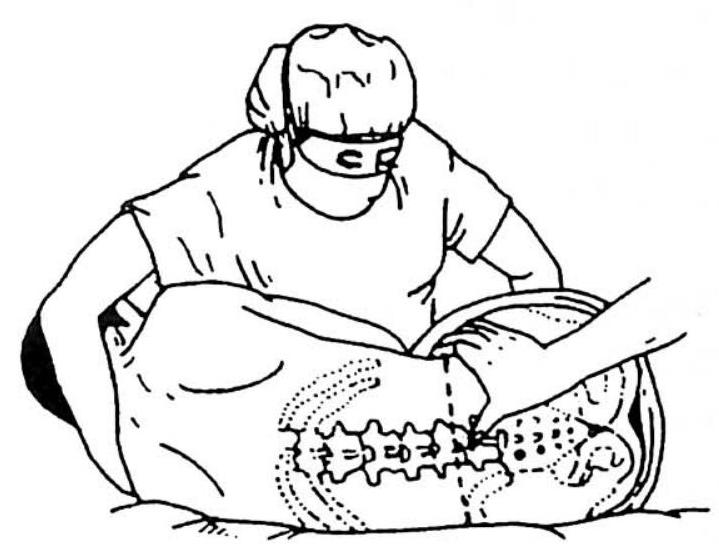
\includegraphics[max width=\textwidth]{2024_07_09_002a177993bd97d1d6d7g-062(1)}
\end{center}

图 4-5 $\quad$ 腰麻穿刺体位和穿刺点定位方法

\begin{center}
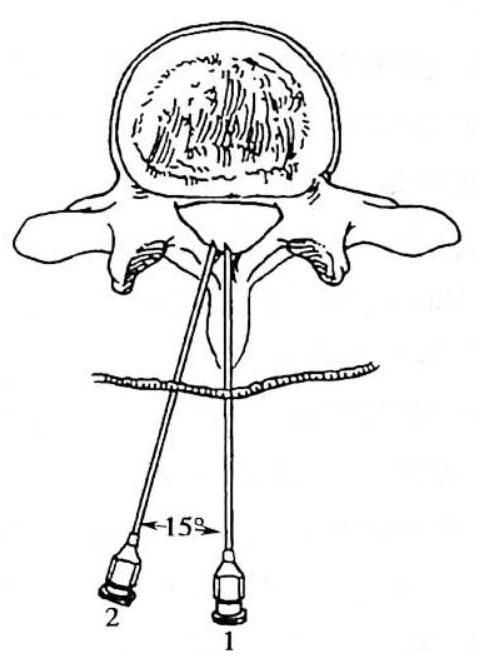
\includegraphics[max width=\textwidth]{2024_07_09_002a177993bd97d1d6d7g-062}
\end{center}

图 4-6 直入法与侧入法

\begin{enumerate}
  \item 直人法; 2 . 侧人法
\end{enumerate}

(1)直人穿刺法: 用左手拇、示指固定穿刺点皮肤。将穿刺针在棘突间隙中点与患者背部垂直、针尖稍向头侧缓慢刺人, 并仔细体会针尖处的阻力变化。当针尖穿过黄韧带时, 有阻力突然消失 “落空” 感觉, 继续推进时常有第二个 “落空” 感觉, 提示已穿破硬脊膜与蛛网膜而进人蛛网膜下隙。

(2) 侧人穿刺法: 于棘突间隙中点旁开 $1.5 \mathrm{~cm}$ 处作局部浸润, 穿刺针与皮肤成 $75^{\circ}$ 角对准棘突间孔刺人, 经黄韧带及硬脊膜而达蛛网膜下陌。本法可避开棘上及棘间韧带, 特别适用于棘上韧带钙化或脊柱畸形的患者。此外,当直人法穿刺未能成功时, 也可改用本方法。

针尖进人蛛网膜下隙后, 拔出针芯即有脑脊液流出; 有时未见脑脊液流出可能系患者脑压过低所致, 可试用压迫颈静脉或让患者屏气等措施, 以促进脑脊液流出; 也可旋转针干 $180^{\circ} \mathrm{C}$, 或用注射器缓慢抽吸。经上述处理仍无脑脊液流出时, 应重新穿刺。穿刺时如遇骨质, 应改变进针方向,避免暴力,以免造成损伤。

\section*{(六)阻滞平面的调节}
阻滞平面是指皮肤感觉消失的界限。临床上常以针刺皮肤测痛的方法来判断, 同时观察运动神经麻痹的进展情况, 也有助于了解其作用范围。如骶神经被阻滞时, 足趾即不能活动, 腰神经被阻滞则不能屈膝。 $\mathrm{T}$, 神经以下被阻滞时, 腹肌松驰, 令患者咳嗽, 可见腹肌松软膨起, 大致判断运动神经纤维被阻滞的平面。

局麻药的剂量大小是决定蛛网膜下弥阻滞平面的主要因素, 影响因素包括:穿刺间隙、患者体位、麻醉药容量和比重、注药速度和针尖斜口方向等。(1)穿刺部位: 由于脊柱有四个生理曲度, 如果经 $\mathrm{L}_{2-3}$ 间隙穿刺注药, 当患者转为仰卧后, 药液将沿着脊柱的坡度向胸段移动, 使麻醉平面偏高。如果在 $\mathrm{L}_{3-4}$ 间陌穿刺注药, 当患者仰卧后, 大部分药液将向骶段方向移动, 骶部及下肢麻醉较好,麻醉平面偏低。(2)患者体位和药液比重:重比重药液向低处扩散,轻比重药液向高处扩散。注药后一般应在 5 10 分钟之内调节患者体位, 以获得所需麻醉平面。(3)注药速度:通常注射的速度愈快,麻醉范围愈广; 相反,注射速度愈慢,药物愈集中,麻醉范围愈小。一般以\\
每 5 秒注人 $1 \mathrm{ml}$ 药液为适宜。鞍区麻醉时,注射速度可减至每 30 秒 $1 \mathrm{ml}$,以使药物集中于骶部。 (4)穿刺针尖斜口方向: 斜口朝向头侧, 麻醉平面易升高; 反之, 麻醉平面不易上升。如果局麻药已经注人, 则只能根据药物比重来调节患者的体位, 以达到预定的麻醉平面。

\section*{(七)麻醉期间的管理}
蛛网膜下腙阻滞后, 可引起一系列生理扰乱, 其程度与阻滞平面密切相关, 平面愈高, 扰乱愈明显。

\begin{enumerate}
  \item 血压下降和心率缓慢 蛛网膜下弥阻滞平面超过 $\mathrm{T}_{4}$ 后, 常出现血压下降, 多数于注药后 15 30 分钟发生, 同时伴心率缓慢。血压下降主要因交感神经节前纤维被阻滞, 使小动脉扩张、周围血管阻力下降, 血液淤积于周围血管、回心血量减少、心排出量下降等造成。心率缓慢是因部分交感神经被阻滞, 迷走神经相对立进所致。处理应首先考虑补充血容量, 可先快速输液 $200 \sim 300 \mathrm{ml}$; 如果无效可静注麻黄碱 $10 \sim 15 \mathrm{mg}$; 对心率缓慢者可静注阿托品 $0.25 \sim 0.5 \mathrm{mg}$ 以拮抗迷走神经的影响。

  \item 呼吸抑制 当胸段脊神经阻滞后可引起肋间肌麻瘰, 表现为胸式呼吸微弱, 腹式呼吸增强; 患者潮气量减少,咳嗽无力, 不能发声, 甚至发绀。遇此情况应迅速吸氧, 或行人工辅助呼吸, 直至肋间肌张力恢复为止。如果发生 “全脊麻” 引起呼吸停止, 血压骤降, 甚至心搏骤停, 应立即施行心肺复苏, 采取气管内插管、机械通气, 胸外心脏按压等抢救措施。

  \item 恶心、呕吐 诱因包括:(1)血压骤降, 使脑供血骤减, 兴奋了呕吐中枢; (2)迷走神经功能元进, 胃肠蠕动增加; (3)手术牵拉内脏。一旦出现恶心、呕吐症状, 应首先检查是否有麻醉平面过高及血压下降,并采取相应治疗措施。

\end{enumerate}

\section*{二、蛛网膜下隙阻滞的并发症}
\begin{enumerate}
  \item 腰麻后头痛 头痛是腰麻后最常见的并发症, 腰麻后头痛的平均发生率外科手术为 $13 \%$, 妇产科为 $18 \%$ 。典型头痛可在穿刺后的 $6 \sim 12$ 小时内发生, 多数发病于腰麻后 $1 \sim 3$ 天, $75 \%$ 病例持续 4 天, $10 \%$ 持续 1 周, 个别可迁延 1 5 个月或更长时间。腰麻后头痛的原因主要系脑脊液经穿刺孔漏出引起颅内压降低和颅内血管扩张所致, 故穿刺针粗细与头痛发生率明显相关。采用 $25 \sim 26 \mathrm{G}$ 穿刺针可显著降低头痛发生率。麻醉后嘱患者仰卧位以减少脑脊液外流,并保证足够睡眠。一旦发生腰麻后头痛, 可依头痛程度分别进行治疗: (1)轻微头痛: 经卧床 $2 \sim 3$天即自行消失; (2)中度头痛: 患者平卧或采用头低位, 每日输液 2000 3000ml, 并应用小剂量镇静药、镇痛药; (3)严重头痛: 除上述措施外, 可行硬膜外间隙充填疗法, 即先抽取自体血 $10 \mathrm{ml}$, 或右旋糖䣲 $15 \sim 30 \mathrm{ml}$, 在 10 秒内经硬膜外穿刺针注人硬膜外间隙, 注后患者平卧 1 小时, 疗效较好。

  \item 尿渚留 由于 $\mathrm{S}_{2-4}$ 的阻滞, 可使膀胱张力丧失, 此时, 膀胱可发生过度充盈, 特别是男性患者。如果术后需大量输液者应在手术前留置导尿管。

  \item 神经并发症 腰麻致神经损害原因包括: 局麻药的组织毒性、意外地带人有害物质及穿刺损伤。

\end{enumerate}

(1) 脑神经受累: 腰麻后脑神经受累的发生率平均为 $0.25 \%$ 。累及第VI对脑神经较多见,约占 $60 \%$, 其次为第的机制相似。多发生于术后 $2 \sim 21$ 天, 症状为剧烈头痛、畏光、眩晕、复视和斜视。治疗除给予适当镇痛药物缓解头痛外, 还应补充维生素 $\mathrm{B}_{1}$ 。

(2)假性脑脊膜炎: 也称无菌性或化学性脑脊膜炎, 发生率约 1:2000, 多在腰麻后 $3 \sim 4$ 天发病, 临床表现主要是头痛及颈项强直, 凯尔尼格征阳性, 有时有复视、晕眩及呕吐。治疗方法与腰麻后头痛相似。

(3)粘连性蛛网膜炎: 急性脑脊膜炎的反应多为渗出性变化, 若炎症刺激严重则继发性地\\
出现增生性改变及纤维化, 此种增生性改变称为粘连性蛛网膜炎。潜伏期为 $1 \sim 2$ 天, 从运动障碍开始, 可发展至完全肢体瘫㾑。多为药物化学刺激所致, 治疗主要是给予促进神经功能恢复的措施。

(4)马尾神经综合征: 发生原因与粘连性蛛网膜炎相同, 患者于腰麻后下肢感觉及运动功能长时间不恢复, 神经系统检查发现骶尾神经受累, 大便失禁及尿道括约肌麻痹, 恢复异常缓慢。

\section*{第三节 硬膜外阻滞}
\section*{一、硬膜外阻滞的临床应用}
\section*{(一)适应证与禁忌证}
硬膜外阻滞主要适用于腹部手术, 颈部、上肢及胸部手术也可应用,但在管理上比较复杂。此外, 凡适于腰麻的下腹部及下肢等部位手术, 均可采用硬膜外阻滞。近年来, 胸科及腹部手术多主张采用全麻复合硬膜外阻滞, 可减少全麻药的应用,使麻醉更加平稳; 留置硬膜外导管可用于术后行患者自控硬膜外镇痛 (patient-controlled epidural analgesia,PCEA)。此外,还可以与腰麻联合应用于分娩镇痛。

硬膜外阻滞对严重贫血、高血压(原发性或特发性高血压)及心脏代偿功能不良者应慎用,严重休克患者应禁用。穿刺部位有炎症或感染病灶者, 也视为禁忌。对呼吸困难的患者也不宜选用颈、胸段硬膜外阻滞。

\section*{(二)麻醉前访视和麻醉前用药}
\begin{enumerate}
  \item 麻醉前访视 目的在于了解病情和手术要求, 决定穿刺部位, 选择局麻药浓度和剂量, 检查患者循环系统功能能否耐受麻醉, 检查脊柱是否有畸形, 穿刺部位是否有感染, 以及麻醉史及药物过敏史、凝血功能、水和电解质平衡等情况。

  \item 麻醉前用药 硬膜外阻滞的局麻药用量较大, 为预防局麻药毒性反应, 术前 $1 \sim 2$ 小时可给予巴比妥类药或苯二氮草类药; 对阻滞平面高、范围大或迷走神经兴奋性高的患者, 应同时加用阿托品, 以防心率减慢。对术前有剧烈疼痛者应适量使用镇痛药。

\end{enumerate}

\section*{(三)常用局麻药(表 4-1)}
表 4-1 硬膜外阻滞常用局麻药的浓度及剂量

\begin{center}
\begin{tabular}{lcccc}
\hline
局麻药 & 浓度(\%) & \begin{tabular}{c}
-次最大剂量 \\
(mg) \\
\end{tabular} & \begin{tabular}{c}
起效时间 \\
(min) \\
\end{tabular} & \begin{tabular}{c}
持续时间 \\
(min) \\
\end{tabular} \\
\hline
氮普㿞卡因 & $2 \sim 3$ & 800 & $10 \sim 15$ & $45 \sim 60$ \\
丁卡因 & $0.2 \sim 0.3$ & 75 & $15 \sim 20$ & $90 \sim 180$ \\
利多卡因 & $1.5 \sim 2.0$ & 400 & $5 \sim 15$ & $80 \sim 120$ \\
布比卡因 & $0.5 \sim 0.75$ & 150 & $10 \sim 20$ & $165 \sim 225$ \\
左布比卡因 & $0.5 \sim 0.75$ & 150 & $10 \sim 20$ & $150 \sim 225$ \\
罗哌卡因 & $0.5 \sim 1.0$ & 200 & $10 \sim 20$ & $140 \sim 180$ \\
\hline
\end{tabular}
\end{center}

\section*{(四)应用局麻药的注意事项}
\begin{enumerate}
  \item 局麻药浓度的选择 决定硬膜外阻滞范围的最主要因素是局麻药的容量, 决定阻滞程度和作用持续时间的主要因素是局麻药的浓度。根据穿刺部位和手术要求不同, 对麻醉药浓度应作适当选择。以利多卡因为例, 颈胸部手术以 $1 \% \sim 1.3 \%$ 为宜, 浓度过高可引起膈肌麻痹; 用于\\
腹部手术为达到腹肌松驰, 需用 $1.5 \% \sim 2 \%$ 浓度。此外, 浓度选择还与患者一般情况有关, 健壮患者所需浓度宜偏高, 虚弱或老年患者浓度应降低, 婴幼儿应用 $1 \%$ 以内的浓度即可取得满意效果。

  \item 注药方法 一般可按下列顺序给药: (1)试验剂量:一般为 $2 \%$ 利多卡因 $3 \sim 5 \mathrm{ml}$, 目的在于排除意外进人蛛网膜下隙的可能。如果注药后 5 分钟内出现下肢痛觉和运动消失,以及血压下降等症状,提示局麻药已进人蛛网膜下隙, 严重时可发生全脊麻, 应立即进行抢救。此外, 从试验剂量所出现的阻滞范围及血压波动幅度,可了解患者对药物的耐受性,以指导继续用药的剂量。(2)追加剂量: 注人试验剂量 5 分钟后, 如无蛛网膜下弥阻滞征象, 方可注人追加剂量。虽然追加剂量的大小因人而异, 给药方法也有不同, 但阻滞范围应能满足手术的要求。试验剂量和追加剂量之和称初量。(3)维持量:术中患者由无痛转而出现痛感,肌肉由松驰转为紧张,应考虑局麻药的阻滞作用开始减退, 可追加维持量, 一般为初量的 $1 / 3 \sim 1 / 2$ 。

\end{enumerate}

\section*{(五)硬膜外间隙穿刺术}
\begin{enumerate}
  \item 体位 分侧卧位及坐位两种, 临床上主要采用侧卧位, 具体要求与蛛网膜下隙阻滞法相同。

  \item 穿刺点的选择 穿刺点应根据手术部位选定,一般取支配手术范围中央的脊神经相应棘突间隙。为确定各棘突的位置, 可参考下列体表解剖标志: (1)颈部最大突起的棘突为第 7 颈椎棘突; (2)两侧肩胛冈连线为第 3 胸椎棘突; (3)肩胛角连线为第 7 胸椎棘突; (4)两侧髂塍最高点的连线为第 4 腰椎棘突或腰 $4-5$ 棘突间隙。临床上可用第 7 颈椎棘突作为标志向尾侧顺数,或以第 4 腰椎棘突为标志向头侧倒数,即可测得穿刺间隙。

  \item 穿刺术 包括直人法和侧人法两种。颈椎、胸椎上段及腰椎的棘突呈平行排列, 多主张用直人法; 胸椎中下段的棘突呈叠瓦状, 间隙狭窄, 穿刺困难时可用侧人法。老年人棘上韧带钙化,脊柱弯曲受限者,一般宜用侧人法。

\end{enumerate}

(1)直人法:在选定的棘突间陌靠近下棘突的上缘处作皮丘,然后再作深层浸润,局麻必须完善,否则疼痛可引起反射性背肌紧张,增加穿刺困难。针的刺人位置必须在脊柱的正中矢状线上。针尖所经的组织层次与腰麻时一样, 穿透黄韧带时有阻力骤然消失感, 提示进人硬膜外间隙。

(2)侧人法:侧人法是在棘突间隙中轴线的中点旁开 $1.5 \mathrm{~cm}$ 处进针, 避开棘上韧带和棘间韧带, 经黄韧带进人硬膜外间隙。操作步骤: 在选定的棘突间隙靠近下棘突旁开 $1.5 \mathrm{~cm}$ 处作皮丘、皮下及肌肉浸润。穿刺针与皮肤成 $45^{\circ} \sim$ $75^{\circ}$ 角对准棘突间孔刺人, 经棘突间孔刺破黄韧带进人硬膜外间弥。

\begin{enumerate}
  \setcounter{enumi}{3}
  \item 硬膜外间隙的确定 穿刺针到达黄韧带后, 根据阻力突然消失、负压的出现以及无脑脊液流出等现象, 即可判断穿刺针已进人硬膜外间隙。
\end{enumerate}

(1)阻力突然消失: 当穿刺针抵达黄韧带时, 阻力增大, 并有韧性感; 将针芯取下, 接上注射器, 推动注射器芯,有回弹感觉,表明针尖已抵达黄韧带; 继续缓慢进针,一旦穿破黄韧带,即有阻力顿时消失的“落空感”, 同时注人生理盐水无阻力,表示针尖已进人硬膜外间隙 (图 4-7)。

(2)负压现象:临床上常用负压现象来判断硬膜外间

\begin{center}
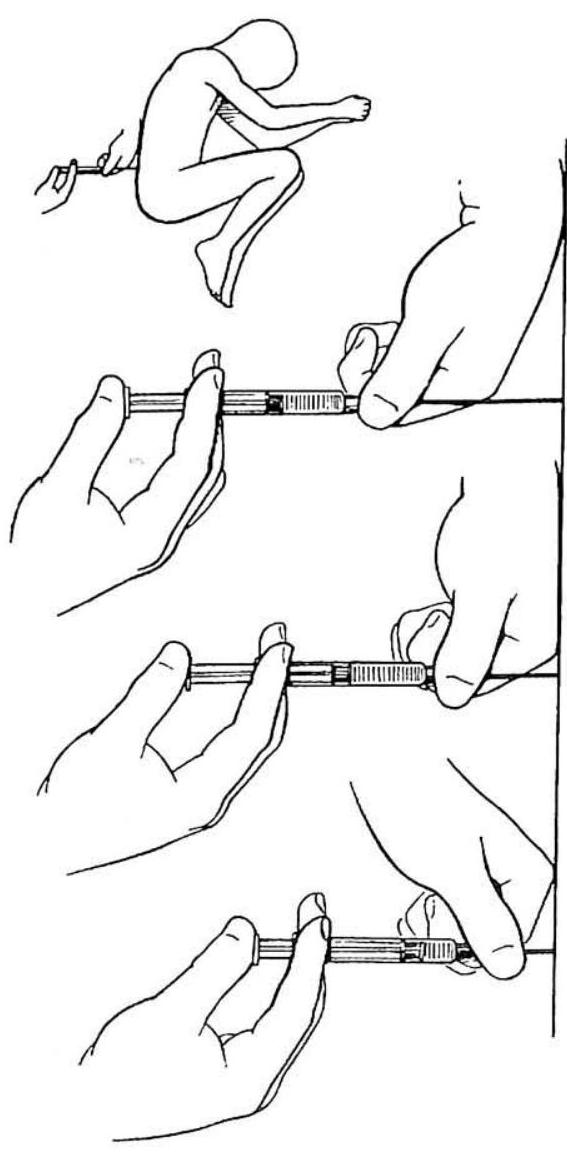
\includegraphics[max width=\textwidth]{2024_07_09_002a177993bd97d1d6d7g-065}
\end{center}

图 4-7 硬膜外穿刺阻力消失示意图\\
隙。当穿刺针抵达黄韧带时, 拔除穿刺针芯, 在针蒂上悬挂一滴生理盐水, 继续缓慢进针。当针尖穿透黄韧带而进人硬膜外间隙时, 可见悬滴被吸人, 此即为负压现象的悬滴法(图 4-8)。负压现象于颈胸段穿刺时比腰段清楚。

\begin{center}
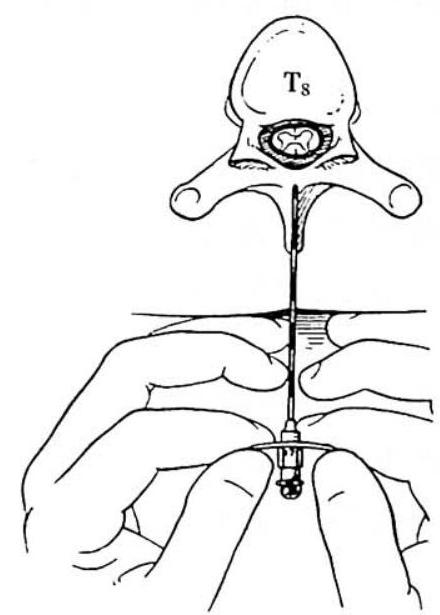
\includegraphics[max width=\textwidth]{2024_07_09_002a177993bd97d1d6d7g-066}
\end{center}

A

\begin{center}
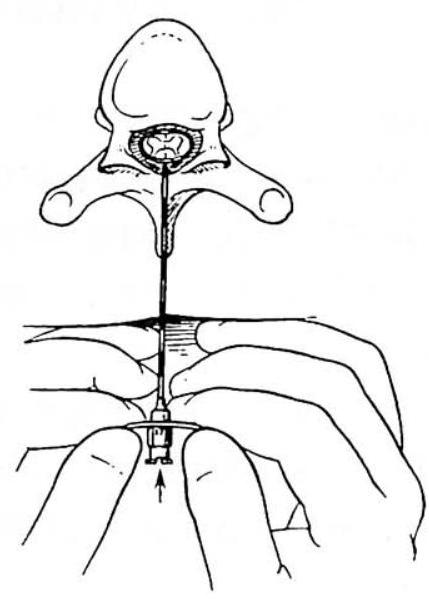
\includegraphics[max width=\textwidth]{2024_07_09_002a177993bd97d1d6d7g-066(1)}
\end{center}

B

图 4-8 悬滴法穿刺示意图

A. 悬滴穿刺;B. 穿刺针进人硬脊膜外院

\section*{(六)连续硬膜外阻滞置管方法}
确定针尖已进人硬膜外间陌后, 即可经针蒂置人硬膜外导管。置管前应根据拟定的置管方向调整好针尖斜面的方向。导管置人长度以 $3 \sim 5 \mathrm{~cm}$ 为宜。

\begin{enumerate}
  \item 置管操作步骤 (1)置管时应先测量从穿刺点皮肤到硬膜外间弥的距离, 即将穿刺针全长减去针蒂至皮肤的距离即得。(2)操作者以左手背贴于患者背部,以拇指和示指固定针蒂, 右手持导管的头端, 经针蒂插人针腔。进至 $10 \mathrm{~cm}$ 处稍有阻力, 表示导管已到达针尖斜口, 稍用力推进, 导管即可滑人硬膜外间隙, 继续缓慢插人 $3 \sim 5 \mathrm{~cm}$, 至导管的 $15 \mathrm{~cm}$ 刻度处停止。(3)拔针时, 应一手退针,另一手固定好导管, 以防将导管带出。在拔针过程中不要随意改变针尖的斜口方向,以防斜口割断导管。(4)调整好导管在硬膜外的长度。如置人过长, 可轻轻将导管向外退拉至预定的刻度。(5)导管尾端接上注射器, 注人少许生理盐水, 无阻力, 回吸无血或脑脊液, 表示导管通畅 , 位置正确, 即可固定导管。

  \item 置管注意事项 (1)导管已越过穿刺针斜口而遇阻力需将导管退出重插时, 必须将导管与穿刺针一并拔出,切忌只拔导管,否则会有针尖斜口割断导管的危险。(2)插管过程中如患者出现肢体异感或弹跳,提示导管已触及脊神经根; 异感严重者, 应将穿刺针与导管一并拔出, 重新穿刺置管。(3)导管内流出全血,提示导管已刺破硬膜外间隙静脉丛,可用含少量肾上腺素的生理盐水作冲洗, 如仍流血时, 应考虑另换间祘作穿刺置管。

\end{enumerate}

\section*{(七)硬膜外阻滞平面的调节}
影响硬膜外阻滞平面的因素很多, 其中最重要的是穿刺部位, 如果选择不当, 将导致阻滞范围不能满足手术要求。此外, 导管的位置和方向、药物容量、注药速度、患者体位以及全身情况等均起重要作用。

\begin{enumerate}
  \item 导管的位置和方向 向头端置管时,药物易向头侧扩散;向尾端置管时,药液多向尾侧扩散。如果导管偏于一侧, 可出现单侧麻醉。如导管误人椎间孔,则只能阻滞单根脊神经。

  \item 药物容量和注药速度 容量愈大,注药速度愈快, 阻滞范围愈广, 反之则阻滞范围较窄。

  \item 体位 硬膜外间弥注人药物, 其扩散很少受体位的影响, 故临床可不必调整体位。

  \item 患者情况 婴幼儿硬膜外间陌窄小,药物易向头侧扩散, 所需药物量小。老年人硬膜外

\end{enumerate}

\section*{第四章 椎管内麻醉}
间隙缩小, 椎间孔狭窄甚至闭锁, 药物的外溢减少, 阻滞范围容易扩大, 用药量须适当减少。临床操作时, 可先注射 $2 \sim 4 \mathrm{ml}$ 作为试验量, 观察阻滞范围大小后再酌情分次减量追加药物。奼娠后期, 由于下腔静脉受压, 硬膜外间隙静脉充盈, 间隙相对变小, 药物容易扩散, 用药量也应减少。有些病理因素, 如全身情况差、脱水、血容量不足、腹内压增高, 可加速药物扩散, 用药量应格外慎重。

\section*{(八)硬膜外阻滞术中患者的管理}
硬膜外间弥注人局麻药 $5 \sim 10$ 分钟内, 在穿刺部位的上下各 2,3 节段的皮肤支配区可出现感觉迟钝,20 分钟内阻滞范围可扩大到所预期的范围, 麻醉也趋完全。由此可引起一系列生理扰乱, 最常见的是血压下降、呼吸抑制和恶心呕吐。因此, 术中应注意麻醉平面, 密切观察病情变化, 及时进行妥善处理。

\begin{enumerate}
  \item 血压下降 多发生于胸段硬膜外阻滞, 由于内脏大小神经麻痹, 导致腹内血管扩张, 回心血量减少而血压下降, 同时副交感神经功能相对六进, 可出现心动过缓。这些变化多于注药后 20 分钟内出现,应先行输液补充血容量, 必要时静注麻黄碱 $10 \sim 15 \mathrm{mg}$ 或去氧肾上腺素 $25 \sim$ $50 \mu \mathrm{g}$, 可获得满意效果。

  \item 呼吸抑制 阻滞平面低于 $\mathrm{T}_{8}$ 对呼吸功能影响很小。颈部及上胸部硬膜外阻滞时, 由于肋间肌和膈肌不同程度麻痹, 可出现呼吸抑制。此外, 颈胸部硬脊膜外隙相对较小, 故应采用小剂量、低浓度局麻药, 以减少对运动神经的阻滞。术中必须仔细观察患者呼吸, 并作好急救准备。

  \item 恶心呕吐 硬膜外阻滞并不能消除牵拉内脏所引起的牵拉痛或牵拉反射, 患者常出现胸闪不适,甚至烦躁、恶心、呕吐, 必要时可静注辅助药物加以控制,如芬太尼 $(50 \mu \mathrm{g})$ 。

\end{enumerate}

\section*{二、硬膜外阻滞的并发症}
\section*{(一)穿破硬脊膜}
\begin{enumerate}
  \item 原因 硬膜外穿刺时穿破硬脊膜的原因有操作因素,也有患者本身的因素。
\end{enumerate}

(1) 操作因素:(1)硬膜外穿刺是一种盲探性操作技术,初学者在穿刺时可能对椎间不同韧带的层次感体会不深; (2)麻醉科医师在穿刺时进针过快, 或遇到骨质而突然滑人; (3)导管质地过硬,也可增加穿破硬脊膜的可能性,且不容易被发现。

(2)患者因素:(1)多次接受硬膜外阻滞,由于反复创伤、出血或药物的化学刺激,硬膜外间隙因粘连而变窄, 往往在穿刺针穿过黄韧带时即可同时穿破硬脊膜; (2)脊柱畸形、病变、腹内巨大肿块或腹水,脊柱不易弯曲而造成穿刺困难, 反复试探性穿刺时有可能穿破硬脊膜; (3)老年人韧带钽化, 常在穿过黄韧带后滑人蛛网膜下隙,故老年人穿破率比年轻人高 2 倍; (4) 因先天性硬脊膜菲薄, 可致穿破率增加; (5)小由于其硬膜外间隙较成人更为狭窄,操作更加困难,且必须在全麻或基础麻醉下进行,更易穿破硬脊膜。

\begin{enumerate}
  \setcounter{enumi}{1}
  \item 处理 一旦硬脊膜被穿破,应改换其他麻醉方法, 如全麻或神经阻滞。如穿刺点在腰 2 以下,手术区域在下腹部、下肢或肛门会阴区者, 可慎用蛛网膜下隙阻滞。
\end{enumerate}

\section*{(二)穿刺针或导管误入血管}
\begin{enumerate}
  \item 硬膜外间隙有丰富的血管丛,穿刺针或导管误人血管并不罕见, 发生率据文献报道在 $0.2 \% \sim 2.8 \%$ 。尤其是足月娃娠者, 因硬膜外间陌静脉怒张, 发生率更高。误人血管会因穿刺针或导管内出血而被发现,少数病例因导管开口处被凝血块阻塞而不易被发现,注药时小凝血块被推开,局麻药便直接注人血管内而发生毒性反应。

  \item 预防措施 (1)导管宜从正中人路置人; (2)导管置放后注局麻药前应轻轻抽吸, 验证有无血液; (3)常规通过导管注人试验剂量局麻药; (4)导管及盛有局麻药的注射器内如有血染, 应警惕导管进人血管内的可能。

  \item 处理 如遇血液由穿刺针或导管流出,可将导管退出 $1 \mathrm{~cm}$ 并以生理盐水 $10 \mathrm{ml}$ 冲洗,多可停止或缓解; 不能缓解者, 或改变间隙重新穿刺, 或改为其他麻醉方法。但有凝血障碍者, 有发生硬膜外血肿的危险, 术后应密切观察, 及时发现和处理。如果导管进入血管内而未及时发现,注人局麻药而引起局麻药毒性反应者, 应立即按局麻药毒性反应处理。

\end{enumerate}

\section*{(三)导管折断}
\begin{enumerate}
  \item 原因 (1)遇导管尖端越过穿刺针斜面后不能继续进人时, 若试图仅将导管退出,导管可能被穿刺针的斜面切断; (2)骨关节炎患者,椎板或棘间韧带将导管夹住,出现拨管困难, 若强力拔出会拉断导管; (3)导管折叠、导管在硬膜外间隙圈绕成结, 导管拔出困难。遇此情况, 须切开各层组织直至折叠或圈结部位, 始能取出。

  \item 处理 由于导管残端可能在硬膜外间隄, 也可能在软组织内, 难以定位, 采取手术取出的创伤较大,手术也不一定能成功。因此,一般都不主张马上手术取出。残留导管一般不会引起并发症, 但事发后应告知患者, 消除顾虑, 取得理解和配合, 同时予以仔细观察和随访。如果术毕即发现导管断端在皮下,可在局麻下作切口取出。

\end{enumerate}

\section*{(四)全脊麻}
行硬膜外阻滞时, 如穿刺针或硬膜外导管误人蛛网膜下陁而未能及时发现, 超过腰麻数倍量的局麻药注人蛛网膜下隙, 可产生异常广泛的阻滞, 产生全脊麻。临床表现为全部脊神经支配的区域均无痛觉、低血压、意识丧失及呼吸停止。全脊麻的症状及体征多在注药后短时间内出现, 若处理不及时可能发生心搏骤停。因此, 应严格操作规程, 不能省略“试验剂量”。

处理原则: (1) 维持患者呼吸和循环功能。如患者神志消失, 应行气管插管和机械通气, 加速输液,必要时给予血管活性药升高血压; (2)如出现心搏骤停, 应立即行心肺复苏。

\section*{(五)脊神经根或脊髓损伤}
\begin{enumerate}
  \item 脊神经根损伤 可因穿刺针直接损伤神经根。穿刺过程中如患者主诉有电击样痛, 并向一侧肢体传导, 应停止进针,避免加重损伤。脊神经根损伤以后根为主,临床表现为受损神经根分布区域烧灼感或疼痛,如损伤胸脊神经根则呈 “束带样痛”, 四肢呈条形分布,可表现为感觉减退或消失。根痛症状的典型伴发现象是脑脊液冲击征, 即咳嗽、喷㖇或用力憋气时疼痛或麻木加重。根痛以损伤后 3 天之内最剧, 然后逐渐减轻, 2 周内多数患者缓解或消失, 遗留片状麻木区也可持续数月以上,可采用对症处理。

  \item 脊髓损伤 穿刺针或导管也可直接损伤脊髓, 当触及脊髓时, 患者肢体有电击样异感。轻者数分钟消失, 重者异感持续不退, 应放弃阻滞麻醉, 以免加重神经并发症。若导管插人脊髓或局麻药注人脊髓, 可造成严重损伤, 甚至横贯性损伤, 患者立即感剧痛, 偶有一过性意识障碍,完全松驰性截瘫。脊髓横贯性损伤时血压偏低而不稳定。严重损伤所致的截痽预后不良。

\end{enumerate}

脊髓损伤早期与脊神经根损伤的鉴别: (1)脊神经根损伤当时有 “触电”或痛感,而脊髓损伤时为剧痛,偶伴一过性意识障碍; (2)脊神经根损伤以感觉障碍为主, 有典型 “根痛”, 很少有运动障碍; (3)脊神经根损伤后感觉缺失仅限于 $1 \sim 2$ 根脊神经支配的皮区, 与穿刺点棘突的平面一致; 而脊髓损伤的感觉障碍与穿刺点不在同一平面, 颈部低一节段, 上胸部低两节段, 下胸部低三节段。

\section*{(六)硬膜外血肿}
硬膜外间隙有丰富的静脉丛, 穿刺出血率约为 $2 \% \sim 6 \%$, 但形成血肿出现并发症者, 发生率仅 $0.0013 \% \sim 0.006 \%$ 。形成血肿的直接原因是穿刺针和置人导管的损伤, 如患者合并凝血功能障碍或服用抗凝药物, 则硬膜外血肿发生的几率增加。硬膜外血肿虽然罕见, 但在硬膜外阻滞并发截痽的原因中却占首位。

临床表现: 开始时背痛, 短时间后出现肌无力及括约肌障碍, 发展至完全截痽。硬膜外阻滞后若出现麻醉作用持久不退, 或消退后再度出现感觉减退、肌无力甚至截瘫等, 为血肿形成压迫\\
脊髓的征兆; 椎管造影、CT 或磁共振对于明确诊断及阻塞部位很有帮助; 脑脊液检查仅蛋白含量略高, 压颈试验提示椎管阻塞。

预后取决于早期诊断和及时手术, 如确诊后尽早 (8 小时内) 行椎板减压术, 清除血肿, 症状多可缓解, 预后较好。如超过 12 小时再行手术, 恢复可能性极小。因此, 对有凝血障碍及正在使用抗凝治疗的患者, 应避免应用硬膜外阻滞; 穿刺操作时应强调避免暴力及反复穿刺。

\section*{三、骶管阻 滞}
骶管阻滞是经骶裂孔穿刺, 将局麻药注人骶管腔内以阻滞骶脊神经, 属硬膜外阻滞。适用于直肠、肛门及会阴部手术, 也用于婴幼儿及学龄前儿童的腹部手术。

\begin{enumerate}
  \item 穿刺点定位方法 从尾骨尖沿中线向头方向 $3 \sim 4 \mathrm{~cm}$ 处 (成人), 可触及一有弹性的 $\mathrm{V}$ 形凹陷, 凹陷两旁可触到蚕豆大骨质隆起的骶角, 位于两骶角连线中点的凹陷即为穿刺点一一骶裂孔(图 4-9)。髂后上棘连线处在第 2 骶椎平面, 是硬脊膜虂的终止部位, 骶管穿刺针如越过此连线, 即有误人蛛网膜下隙发生全脊麻的危险。

  \item 穿刺与注药 患者取侧卧位或俯卧位。侧卧位时, 腰背应尽量向后弓曲, 双膝屈向腹部。俯卧位时, 髋部需垫厚枕以抬高骨盆, 暴露骶部。于骶裂孔中心作皮内小丘, 但不作皮下浸润, 否则将使骨质标志不清, 妨碍穿刺点定位。将穿刺针垂直刺进皮肤, 当刺破骶尾韧带时可有阻力消失感觉。此时将针干向尾侧倾斜, 与皮肤呈 $30^{\circ} \sim 45^{\circ}$ 角顺势推进 $2 \mathrm{~cm}$ 即可到达骶管腔。接上注射器, 抽吸无脑脊液, 注射生理盐水和空气无阻力, 也无皮肤隆起,证实针尖确在骶管空内, 即可注人试验剂量。观察 5 分钟内无蛛网膜下隙阻滞现象, 即可分次注人其余药液。

\end{enumerate}

穿刺成功的要点在于掌握好穿刺针的方向。如果针与尾侧皮肤角度过小, 即针体过度放平,针尖可在骶管的后壁受阻; 若角度过大, 针尖常可触及骶管前壁。

\begin{center}
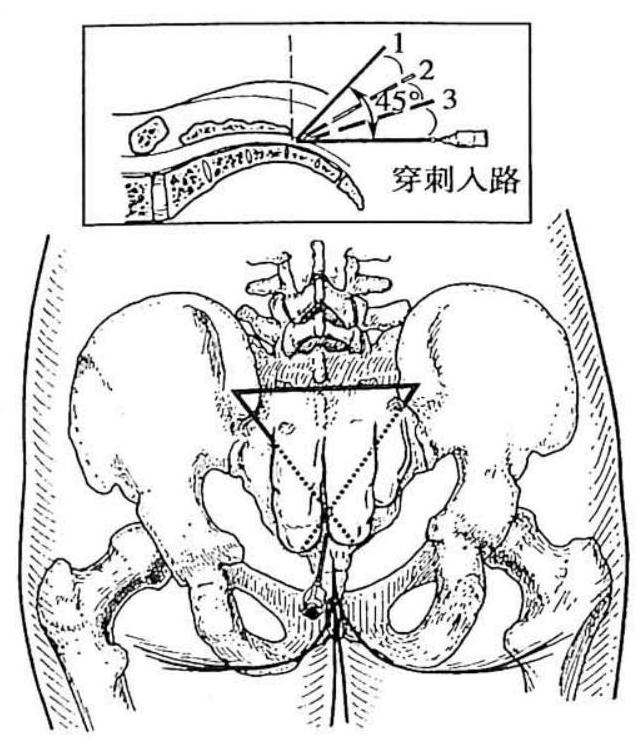
\includegraphics[max width=\textwidth]{2024_07_09_002a177993bd97d1d6d7g-069}
\end{center}

图 4-9 骶管穿刺技术示意图穿刺时如遇骨质, 不宜用暴力, 应退针少许, 调整针体倾斜度后再进针, 以免引起剧痛和损伤骶管静脉丛。当抽吸有较多回血时, 应放弃骶管阻滞, 改用腰部硬膜外阻滞。

\begin{enumerate}
  \setcounter{enumi}{2}
  \item 常用局麻药 常采用 $1 \% \sim 1.5 \%$ 利多卡因、 $0.5 \%$ 布比卡因或 $0.5 \%$ 罗哌卡因, 注人局麻药 $15 \sim 20 \mathrm{ml}$ 即可满足骶管阻滞的麻醉效果。

  \item 并发症 骶管腔内有丰富的静脉丛, 穿刺时容易出血。对局麻药的吸收也快, 易产生局麻药毒性反应。如注药过快, 则可能导致眩晕和头痛。因骶裂孔解剖变异较多, 故阻滞的失败率较高。由于骶神经阻滞时间较长, 术后尿渚留较多。

\end{enumerate}

\section*{第四节 蛛网膜下隙-硬膜外联合阻滞}
蛛网膜下弥-硬膜外联合阻滞 (combined spinal-epidural anesthesia, CSEA; 简称腰麻-硬膜外联合阻滞) 近年来已广泛应用于经腹、盆腔手术, 并取得满意效果。经腹、盆腔手术要求麻醉应充分镇痛与肌松, 因此常需较广泛阻滞, 麻醉上界需达 $\mathrm{T}_{6}$, 下界需达 $\mathrm{S}_{4}$, 手术时间长。如采用硬膜外阻滞, 需选用双管法连续硬膜外阻滞, 此法不仅操作复杂, 局麻药用量也多, 部分患者仍存在盆腔内脏牵拉反应, 常需辅助大量镇痛药方能完成手术操作。腰麻-硬膜外联合阻滞既保留了腰麻起效快、镇痛完善与肌松良好的优点, 也便于调节麻醉平面, 防止麻醉平面过高。经硬膜外导\\
管追加局麻药可弥补单纯腰麻阻滞平面不足或阻滞时间不够的缺点。

腰麻-硬膜外联合阻滞可选用两点穿刺法,也可采用一点穿刺方法。既向蛛网膜下隙注药,同时也经此穿刺针置人硬膜外导管。两点法穿刺时,先根据手术部位选择合适的穿刺间隙行硬膜外穿刺, 留置硬膜外导管备用; 然后再于 $\mathrm{L}_{2-3}$ 或 $\mathrm{L}_{3-4}$ 行蛛网膜下隙穿刺, 注局麻药行腰麻。一点穿刺法时,应用特制的联合穿刺针选择经 $\mathrm{L}_{2-3}$ 间隙穿刺。当硬膜外穿刺成功后, 用 $25 \mathrm{G}$ 腰麻针经硬膜外穿刺针管腔内行腰麻穿刺; 当脑脊液流出后, 将所需局麻药注入蛛网膜下隙 (腰麻);然后退出腰麻穿刺针, 再经硬膜外穿刺针向头端置人硬膜外导管 $3 \sim 5 \mathrm{~cm}$, 置管后将硬膜外穿刺针退出,并将硬膜外导管妥为固定 (图 4-10)。\\
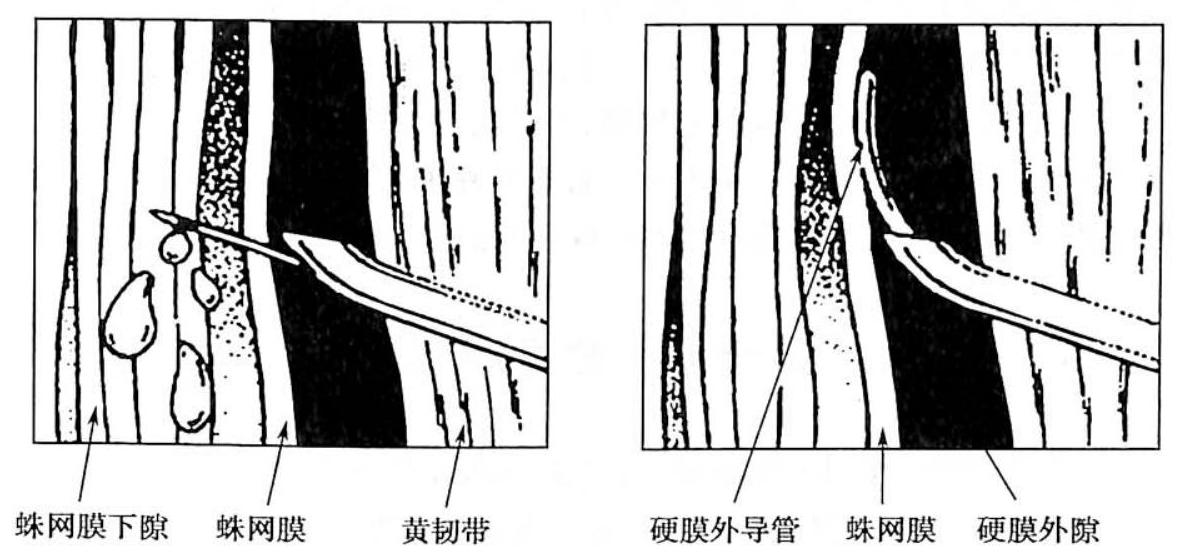
\includegraphics[max width=\textwidth, center]{2024_07_09_002a177993bd97d1d6d7g-070}

图 4-10 腰麻-硬膜外联合阻滞示意图

腰麻-硬膜外联合阻滞时所用的腰麻穿刺针较细, 注药时间需 $45 \sim 60$ 秒, 但腰麻与硬膜外用药量均较两点穿刺法为少。一点穿刺法对患者的损伤小, 由于采用 $25 \mathrm{G}$ 腰麻穿刺针, 术后头疼发生率也明显减低。应用 CSEA 的优点见表 4-2。

表 4-2 CSEA 的优点

\begin{enumerate}
  \item 由硬膜外穿刺针引导腰麻针穿刺至蛛网膜下隙, 减少了腰麻针碰到骨面而使针尖变钝的可能

  \item 经硬膜外导管给药不仅可补充腰麻时间有限的不足, 并可用于术后镇痛

  \item 与单纯硬膜外阻滞比较, 腰麻起效快, 阻滞完善, 可使手术较早开始

  \item 腰麻用药量小,可降低局麻药血药浓度,减少对生理的干扰; 必要时经硬膜外给药,可提高阻滞平面

  \item 用于分娩镇痛时, 可经腰麻针先向蛛网膜下隙注人小剂量阿片类药物, 需要时再经硬膜外导管追加镇痛药和局麻药

\end{enumerate}

\section*{第五章 全 身麻 醉}
麻醉药经呼吸道吸人或静脉、肌内注射进人人体, 产生中枢神经系统的抑制, 临床表现为神志消失、全身的痛觉丧失、遗忘、反射抑制和一定程度的肌肉松驰, 这种方法称为全身麻醉。麻醉药对中枢神经系统抑制的程度与血液内的药物浓度有关, 并且可以调控。这种抑制是完全可逆的, 当药物被代谢或从体内排出后, 患者的神志、感觉和各种反射逐渐恢复。为了确保患者的安全,全身麻醉时一般都要求建立人工气道。对于短小手术、容易保持气道通畅者, 也可不建立人工气道。由于患者呼吸道的通畅性没有保障, 且不易实施有效的人工呼吸, 因此不建立人工气道的全身麻醉可能更危险。全身麻醉不同于普通的睡眠, 全身麻醉对中枢神经系统, 呼吸、循环系统以及对伤害性刺激的反应等均产生不同程度的抑制, 甚至消失。

\section*{第一节 全身麻醉药}
根据用药途径和药物的作用机制不同, 可将全身麻醉药分为吸人麻醉药、静脉麻醉药。肌肉松驰药 (简称 “肌松药”) 和麻醉性镇痛药一般视为全麻辅佐用药。

\section*{一、吸人麻醉药}
吸人麻醉药 (inhalation anesthetics) 是指经呼吸道吸人人体内并产生全身麻醉作用的药物。可用于全身麻醉的诱导和维持。

\section*{(一)理化性质与药理性能}
现今常用的吸人麻醉药多为卤素类,经呼吸道吸人后, 通过与脑细胞膜的相互作用而产生全身麻醉作用。吸人麻醉药的强度是以最低肺泡浓度 (minimum alveolar concentration, MAC) 来衡量的。MAC 是指某种吸人麻醉药在一个大气压下与纯氧同时吸人时, 能使 $50 \%$ 患者在切皮时不发生摇头、四肢运动等反应时的最低肺泡浓度。因为 MAC 是不同麻醉药的等效价浓度, 所以能反映麻醉药的效能, 麻醉药的 MAC 越小其麻醉效能越强。吸人麻醉药的油/气分配系数 (即脂溶性)和血/气分配系数(即药物在血液中的溶解度)对其药理性能有明显影响。由表 5-1 可见, 吸人麻醉药的强度与其油/气分配系数呈正比关系, 油/气分配系数越高, 麻醉强度越大, MAC 则越小。麻醉深度与脑内吸人麻醉药的分压相关, 当肺泡、血液和脑组织中的吸人麻醉药分压达到平衡时,肺泡药物浓度 $\left(\mathrm{F}_{\mathrm{A}}\right)$ 则可反映吸人麻醉药在脑内的分布情况。吸人麻醉药的可

表 5-1 吸入麻醉药的理化性质

\begin{center}
\begin{tabular}{lccccc}
\hline
药物 & 分子量 & 油/气 & 血/气 & 代谢率(\%) & MAC(\%) \\
\hline
乙醚 & 74 & 65 & 12 & $2.1 \sim 3.6$ & 1.9 \\
氧化亚氮 & 44 & 1.4 & 0.47 & 0.004 & 105 \\
氟烷 & 197 & 224 & 2.4 & $15 \sim 20$ & 0.75 \\
恩氟烷 & 184 & 98 & 1.9 & $2 \sim 5$ & 1.7 \\
异氟烷 & 184 & 98 & 1.4 & 0.2 & 1.15 \\
七莪烷 & 200 & 53.4 & 0.65 & $2 \sim 3$ & 2.0 \\
地樉烷 & 168 & 18.7 & 0.42 & 0.02 & 6.0 \\
\hline
\end{tabular}
\end{center}

控性与其血/气分配系数相关,血/气分配系数越低者,在肺泡、血液和脑组织中的分压达到平衡状态的时间越短,因而在中枢神经系统内的浓度越容易控制。因此,氧化亚氮(笑气)、地氟烷和七氟烷的血/气分配系数较低,其诱导和恢复的速度都较快。

\section*{(二)影响肺泡药物浓度的因素}
吸人麻醉药是通过麻醉机以流经吸人麻醉药蒸发器的新鲜气流为载体, 将麻醉药带人呼吸环路进人呼吸道和肺泡内, 使肺泡中吸人麻醉药的分压上升。在分压差的驱动下, 吸人麻醉药以弥散的方式跨过肺泡膜进人流经肺泡的血液内 (即肺循环对药物的摄取), 并通过血液循环将药物转运到中枢神经系统或其他组织。停止吸人麻醉药后, 吸人麻醉药又以弥散方式由体内各器官和组织进人静脉血, 弥散到肺泡气内, 再经过呼吸道排出到体外。肺泡药物浓度 $\left(\mathrm{F}_{\mathrm{A}}\right)$ 是指吸人麻醉药在肺泡内的浓度, 而吸人药物浓度 $\left(F_{1}\right)$ 是指从环路进人呼吸道的药物浓度。临床上常以 $F_{A}$ 和 $F_{A} / F_{1}$ 来比较不同药物肺泡浓度上升的速度。 $F_{A}$ 和 $F_{A} / F_{1}$ 的上升速度取决于麻醉药的输送和由肺循环摄取的速度。影响因素有:

\begin{enumerate}
  \item 通气效应 肺泡通气量增加, 可将更多的药物输送到肺泡以补偿肺循环对药物的摄取, 结果加速了 $F_{A}$ 升高和 $F_{A} / F_{1}$ 上升的速度。药物的血/气分配系数越大, 被血液摄取量也越多。因此, 对于血/气分配系数大的药物来说, 通气量增加对 $\mathrm{F}_{\mathrm{A}}$ 升高和 $\mathrm{FA} / \mathrm{F}_{1}$ 上升的影响则更明显。

  \item 浓度效应 吸人药物浓度 $\left(\mathrm{F}_{1}\right)$ 不仅可影响 $\mathrm{F}_{\mathrm{A}}$ 的高低, 而且影响 $\mathrm{F}_{\mathrm{A}}$ 上升的速度, 即 $\mathrm{F}_{1}$ 越高, $\mathrm{F}_{\mathrm{A}}$ 上升越快, 称为浓度效应。假如吸人浓度为 $100 \%$ (为假设的理论数值, 因为还需同时吸氧), $\mathrm{F}_{\mathrm{A}}$ 上升非常快。因为这时 $\mathrm{F}_{\mathrm{A}}$ 只取决于肺泡通气时向肺内输送气体的速度, 肺循环对药物的摄取已不能限制 $F_{A} / F_{1}$ 的上升速度。

  \item 心排出量 (CO) 麻醉药是在分压差的驱动下, 以弥散方式由肺泡向血液转移的。在肺泡通气量不变时, 心排出量增加, 通过肺循环的血流量也增加, 被血液摄取并移走的麻醉药也增加, 结果 $\mathrm{F}_{\mathrm{A}}$ 上升减慢。心排出量对 $\mathrm{F}_{\mathrm{A}}$ 的影响, 还与药物的血/ 气分配系数有关, 血/气分配系数越大,心排出量增加引起的血液摄取量也越多, $\mathrm{F}_{\mathrm{A}}$ 降低也越明显。

  \item 血/气分配系数 血/气分配系数越高, 被血液摄取的麻醉药越多, $\mathrm{F}_{\mathrm{A}}$ 上升减慢, 麻醉诱导期延长, 麻醉恢复也较慢。从临床角度讲, 血/气分配系数越低表示麻醉诱导期 $\mathrm{F}_{\mathrm{A}}$ 上升快, 麻醉恢复期 $\mathrm{F}_{\mathrm{A}}$ 降低快, 肺泡、血液和脑组织之间容易达到平衡, 麻醉深度容易控制。吸人麻醉药的可控性与血/气分配系数呈反比关系。

  \item 麻醉药在肺泡和静脉血中的浓度差 $\left(F_{A-V}\right) \quad F_{A-V}$ 越大, 肺循环摄取的药量越多, 即肺血从肺泡带走的麻醉药越多。在麻醉诱导早期, 混合静脉血中的麻醉药接近零, $\mathrm{F}_{A-V}$ 很大, 促进了血液对麻醉药的摄取。随着麻醉的加深和时间的延长, 静脉血中麻醉药浓度增加, 使 $\mathrm{F}_{\mathrm{A}-\mathrm{v}}$ 降低, 摄取速度减慢, 摄取量亦减少, 最终达到相对稳定状态。

\end{enumerate}

\section*{(三)代谢和毒性}
大多数吸人麻醉药的脂溶性较大,很难以原型由肾脏排出,绝大部分由呼吸道排出,仅小部分在体内代谢后随尿排出。药物的主要代谢场所是肝脏, 细胞色素 P450 是重要的药物氧化代谢酶, 能加速药物的氧化代谢过程。此外, 有些药物具有药物代谢酶诱导作用, 可加快其自身代谢速度。药物的代谢过程及其代谢产物对肝脏和肾脏的功能都有不同程度的影响, 影响的程度与药物代谢率和代谢中间产物及最终产物的毒性有关。一般来说,药物的代谢率越低,其毒性也越低。从表 5-1 可见,地氟烷和㫒氟烷的代谢率最低, 因而其毒性也最低, 恩氟烷和七氟烷次之, 而氟烷最高。产生肾毒性的原因主要是血中无机氟 $\left(\mathrm{F}^{-}\right)$浓度的升高。一般认为,当 $\mathrm{F}^{-}$浓度低于 $50 \mu \mathrm{mol} / \mathrm{L}$ 时不产生肾毒性; $50 \sim 100 \mu \mathrm{mol} / \mathrm{L}$ 有引起肾毒性的可能; 而高于 $100 \mu \mathrm{mol} / \mathrm{L}$ 则肯定产生肾毒性。在酶诱导下, F-浓度可显著升高。因此,对慢性肾功能不全或应用酶诱导药物者,应慎用卤素类吸人麻醉药。

\section*{第五章 全 身麻 醉}
\section*{(四)常用吸入麻醉药}
\begin{enumerate}
  \item 氧化亚氮 (nitrous oxide, $\mathrm{N}_{2} \mathrm{O}$, 笑气) 为麻醉性能较弱的气体麻醉药, 推算其 $\mathrm{MAC}$ 为 $105 \%$ 。吸人浓度大于 $60 \%$ 时可产生遗忘作用。氧化亚氮对心肌有一定的直接抑制作用, 但对心排出量、心率和血压都无明显影响, 可能与其可兴奋交感神经系统有关。对肺血管平滑肌有收缩作用,使肺血管阻力增加而导致右房压升高, 但对外周血管阻力无明显影响。对呼吸有轻度抑制作用,使潮气量降低和呼吸频率加快, 但对呼吸道无刺激性,对肺组织无损害。因其血/气分配系数很低, 肺泡浓度和吸人浓度的平衡速度非常快, 肺泡通气量或心排出量的改变对肺循环摄取 $\mathrm{N}_{2} \mathrm{O}$ 的速度无明显影响。 $\mathrm{N}_{2} \mathrm{O}$ 可引起脑血流量增加而使倾内压轻度升高。 $\mathrm{N}_{2} \mathrm{O}$ 几乎全部以原型由呼吸道排出, 对肝肾功能无明显影响。
\end{enumerate}

临床应用:常与其他全麻药复合应用于麻醉维持, 常用吸人浓度为 50\% 70\%。吸人 $50 \%$ $\mathrm{N}_{2} \mathrm{O}$ 可用于牙科或产科镇痛。麻醉时必须维持吸人氧浓度 $\left(\mathrm{FiO}_{2}\right)$ 高于 0.3 , 以免发生低氧血症。在 $\mathrm{N}_{2} \mathrm{O}$ 麻醉恢复期有发生弥散性缺氧的可能, 停止吸 $\mathrm{N}_{2} \mathrm{O}$ 后应吸纯氧 $5 \sim 10$ 分钟。 $\mathrm{N}_{2} \mathrm{O}$ 可使体内封闭腔( 如中耳、肠腔等) 内压升高, 因此气胸、肠梗阻、体外循环以及胸腔镜、腹腔镜等手术不宜应用。

\begin{enumerate}
  \setcounter{enumi}{1}
  \item 恩氟烷 (enflurane) 麻醉性能较强。恩氟烷对中枢神经系统(CNS) 有抑制作用, 随着吸入浓度逐渐升高 (>3\%), 脑电图 (EEG) 可出现嘭症样棘波和爆发性抑制。对心肌收缩力有抑制作用,引起血压、心排出量和心肌氧耗量降低。对外周血管有轻度舒张作用, 导致血压下降和反射性心率增快。虽然恩氟烷也可引起心肌对儿茶酚胺的敏感性增加, 但肾上腺素的用量达 $4.5 \mu \mathrm{g} / \mathrm{kg}$ 时仍不至引起心律失常。对呼吸道无刺激性, 不引起唾液和气道分泌物的增加。对呼吸的抑制作用较强, 表现为潮气量降低和呼吸频率增快。可增强非去极化肌松药的作用。主要代谢产物 $\mathrm{F}^{-}$有肾毒性, 长期应用异烟肼治疗者及肥胖患者吸人恩氟烷后, 血浆中的 $\mathrm{F}^{-}$浓度可增加;但一般临床麻醉后,血浆 F・浓度低于肾毒性阈值。
\end{enumerate}

临床应用:常用于麻醉的维持,维持期的吸人浓度为 $0.5 \% \sim 2 \%$ 。恩氟烷可使眼内压降低,对眼内手术有利。因深麻醉时脑电图显示瘚痛样发作, 临床表现为面部及肌肉抽搐, 因此有㿎病病史者应慎用。

\begin{enumerate}
  \setcounter{enumi}{2}
  \item 异氟烷 (isoflurane)麻醉性能强。异氟烷在低浓度时对脑血流无影响, 高浓度时 (>1MAC) 可使脑血管扩张、脑血流增加和赌内压升高。对心肌收缩力的抑制作用较轻, 对心排出量的影响较小, 但可明显降低外周血管阻力而降低动脉压; 不增加心肌对外源性儿茶酚胺的敏感性。对呼吸有轻度抑制作用,对支气管平滑肌有舒张作用。可增强非去极化肌松药的作用。代谢率很低, 最终代谢产物为三氟乙酸。临床麻醉时血浆最高 $\mathrm{F}^{-}$浓度低于 $10 \mu \mathrm{mol} / \mathrm{L}$; 应用酶诱导剂时, 肝内代谢和 $\mathrm{F}^{-}$浓度无明显增加。因此, 对肝肾功能无明显影响。
\end{enumerate}

临床应用: 常用于麻醉的维持。吸人浓度为 $0.5 \% \sim 2 \%$ 时, 可保持循环功能稳定; 停药后苏醒较快, 约 10 15 分钟。因其对心肌收缩力抑制轻微, 而对外周血管扩张明显, 因而可用于控制性降压。

\begin{enumerate}
  \setcounter{enumi}{3}
  \item 七氟烷(sevoflurane) 麻醉性能较强。七氟烷对 CNS 有抑制作用, 对脑血管有舒张作用, 可引起顾内压升高。对心肌收缩力有轻度抑制, 可降低外周血管阻力, 引起动脉压和心排出量降低。对心肌传导系统无影响, 不增加心肌对外源性儿茶酚胺的敏感性。在 1.5MAC 以上时对冠状动脉有明显舒张作用, 有引起冠脉窃流的可能。对呼吸道无刺激性, 不增加呼吸道的分泌物。对呼吸的抑制作用比较强, 对气管平滑肌有舒张作用。可增强非去极化肌松药的作用,并延长其作用时间。主要在肝脏代谢, 产生 $\mathrm{F}^{-}$和有机氟, 临床麻醉后, 血浆 $\mathrm{F}^{-}$浓度一般为 $20 \sim$ $30 \mu \mathrm{mol} / \mathrm{L}$, 低于肾毒性阈值。
\end{enumerate}

临床应用: 可用于麻醉诱导和维持。用面罩诱导时, 呛咳和屏气的发生率很低。维持麻醉

8.6 分钟。苏醒过程平稳, 恶心和呕吐的发生率低。但在钠石灰中可发生分解, 尤其在钠石灰干燥和温度升高时。

\begin{enumerate}
  \setcounter{enumi}{4}
  \item 地氟烷(desflurane) 麻醉性能较弱。可抑制大脑皮层的电活动, 降低脑氧代谢率; 低浓度虽不抑制中枢对 $\mathrm{CO}_{2}$ 的反应, 但过度通气时也不使顽内压降低; 高浓度可使脑血管舒张, 并降低其自身调节能力。对心肌收缩力有轻度抑制作用, 对心率、血压和心排出量影响较轻; 当浓度增加时, 可引起外周血管阻力降低和血压下降。不增加心肌对外源性儿茶酚胺的敏感性。对呼吸有轻度抑制作用, 可抑制机体对 $\mathrm{PaCO}_{2}$ 升高的反应, 对呼吸道也有轻度刺激作用。对神经肌肉接头有抑制作用,可增强非去极化肌松药的效应。几乎全部由肺排出,除长时间或高浓度应用外,其体内代谢率极低, 因而其肝、肾毒性很低。
\end{enumerate}

临床应用:可单独以面罩诱导, 也可单独或与 $\mathrm{N}_{2} \mathrm{O}$ 合用维持麻醉, 麻醉深度可控性强, 肌松药用量减少。因对循环功能的影响较小, 对心脏手术或心脏病患者行非心脏手术的麻醉或可更为有利。因其诱导和苏醒迅速, 也适用于门诊手术患者的麻醉, 而且恶心和呕吐的发生率明显低于其他吸人麻醉药。但需要特殊的蒸发器, 价格也较贵。

\section*{二、静脉麻醉药}
经静脉注射进人体内, 通过血液循环作用于中枢神经系统而产生全身麻醉作用的药物, 称为静脉麻醉药 (intravenous anesthetics)。其优点为诱导快, 对呼吸道无刺激, 无环境污染。常用静脉麻醉药有:

\begin{enumerate}
  \item 硫喷妥钠 ( thiopental sodium) 为超短效巴比妥类静脉全麻药。常用浓度为 $2.5 \%$, 其水溶液呈强碱性, $\mathrm{pH}$ 为 $10 \sim 11$ 。硫喷妥钠容易透过血脑屏障, 增强脑内抑制性递质 $\gamma$-氨基丁酸 (GABA) 的抑制作用, 从而影响突触的传导, 抑制网状结构的上行激活系统。小剂量静脉注射有镇静、催眠作用; 剂量稍大 $(3 \sim 5 \mathrm{mg} / \mathrm{kg})$ 时, 20 秒内即可使患者人睡。可降低脑代谢率及氧耗量, 降低脑血流量和颅内压。有直接抑制心肌及扩张血管作用而使血压下降, 血压下降程度与所用剂量及注射速度有关; 在合并低血容量或心功能障碍者, 血压降低则更加显著。有较强的中枢性呼吸抑制作用, 表现为潮气量降低和呼吸频率减慢, 甚至呼吸暂停。可抑制交感神经而使副交感神经作用相对增强,使咽喉及支气管的敏感性增加,因此对喉头、气管或支气管的刺激, 容易引起喉痉挛及支气管痉挛。主要在肝脏代谢降解, 肝功能障碍者的麻醉后清醒时间可能延长。
\end{enumerate}

临床应用: (1)全麻诱导: 常用剂量为 $4 \sim 6 \mathrm{mg} / \mathrm{kg}$, 辅以肌松药即可完成气管内插管; (2)控制惊厥: 静注 $2.5 \%$ 溶液 $1 \sim 2 \mathrm{mg} / \mathrm{kg}$; 3 )小儿基础麻醉。

\begin{enumerate}
  \setcounter{enumi}{1}
  \item 氮胺酮 (ketamine) 为苯环已哌啶的衍生物, 易溶于水, 水溶液 $\mathrm{pH}$ 为 $3.5 \sim 5.5$ 。主要选择性抑制大脑联络径路和丘脑-新皮质系统,兴奋边缘系统,而对脑干网状结构的影响较轻。镇痛作用显著;静脉注射后 $30 \sim 60$ 秒患者意识消失,作用时间约 $15 \sim 20$ 分钟; 肌内注射后约 5 分钟起效, 15 分钟作用最强。可增加脑血流量、顾内压及脑代谢率。氯胺酮有兴奋交感神经作用,使心率增快、血压及肺动脉压升高; 而对低血容量性休克及交感神经呈高度兴奋者,氯胺酮可呈现心肌抑制作用。对呼吸的影响较轻, 但用量过大或注射速度过快, 或与其他麻醉性镇痛药伍用时, 可引起显著的呼吸抑制, 甚至呼吸暂停。氯胺酮可使唾液和支气管分泌物增加, 对支气管平滑肌有松驰作用。主要在肝脏内代谢, 代谢产物去甲氯胺酮仍具有一定生物活性, 最终代谢产物由肾脏排出。
\end{enumerate}

临床应用:全麻诱导剂量为 $1 \sim 2 \mathrm{mg} / \mathrm{kg}$ (静脉注射); 麻醉维持量为 $15 \sim 45 \mu \mathrm{g} /(\mathrm{kg} \cdot \mathrm{min}$ )。小儿基础麻醉时, 肌注 $5 \sim 10 \mathrm{mg} / \mathrm{kg}$ 可维持麻醉 30 分钟左右。主要副作用: 可引起一过性呼吸暂停;幻觉、㕵梦及精神症状; 眼内压和颅内压升高。

\begin{enumerate}
  \setcounter{enumi}{2}
  \item 依托咪酯 (etomidate) 为短效催眠药,无镇痛作用,作用方式与巴比妥类近似。起效快,
\end{enumerate}

\section*{第五章 全 身麻 醉}
静脉注射后约 30 秒患者意识即可消失,1 分钟时脑内浓度达峰值。可降低脑血流量、颎内压及脑代谢率。对心率、血压及心排出量的影响均很小; 不增加心肌氧耗量, 并有轻度冠状动脉扩张作用。对呼吸的影响明显轻于硫喷妥钠。主要在肝脏内水解, 代谢产物不具有活性。对肝肾功能无明显影响。

临床应用:主要用于全麻诱导, 适用于年老体弱和危重患者的麻醉,一般剂量为 $0.15 \sim$ $0.3 \mathrm{mg} / \mathrm{kg}$ 。副作用: 注射后常发生肌阵挛;对静脉有刺激性;术后易发生恶心、呕吐; 反复用药或持续静滴后可能抑制肾上腺皮质功能。

\begin{enumerate}
  \setcounter{enumi}{3}
  \item 丙泊酚 (propofol, 异丙酚) 具有镇静、催眠作用,有轻微镇痛作用。起效快,静脉注射 $1.5 \sim 2 \mathrm{mg} / \mathrm{kg}$ 后 $30 \sim 40$ 秒患者即人睡, 维持时间仅为 $3 \sim 10$ 分钟, 停药后苏醒快而完全。可降低脑血流量、须内压和脑代谢率。丙泊酚对心血管系统有明显的抑制作用,抑制程度比等效剂量的硫偾妥钠为重。主要表现为对心肌的直接抑制作用及血管舒张作用,结果导致明显的血压下降、心率减慢、外周阻力和心排出量降低。当大剂量、快速注射, 或用于低血容量者及老年人时, 有引起严重低血压的危险。对呼吸有明显抑制作用, 表现为潮气量降低和呼吸频率减慢, 甚至呼吸暂停, 抑制程度与剂量相关。经肝脏代谢, 代谢产物无生物活性。反复注射或静脉持续输注时体内有蓄积, 但对肝肾功能无明显影响。
\end{enumerate}

临床应用:全麻静脉诱导, 剂量为 $1.5 \sim 2.5 \mathrm{mg} / \mathrm{kg}$ 。可静脉持续输注与其他全麻药复合应用于麻醉维持, 用量为 $6 \sim 10 \mathrm{mg} /(\mathrm{kg} \cdot \mathrm{h})$ 。用于门诊手术的麻醉具有较大优越性, 用量约为 $2 \mathrm{mg} /$ $(\mathrm{kg} \cdot \mathrm{h})$, 停药后 10 分钟患者可回答问题。副作用:对静脉有刺激作用; 对呼吸有抑制作用, 必要时应行人工辅助呼吸; 麻醉后恶心、呕吐的发生率约为 $2 \% \sim 5 \%$ 。

\section*{三、肌肉松驰药}
肌肉松驰药 (muscle relaxants)简称肌松药, 能阻断神经肌肉传导功能而使骨骼肌松驰。自从 1942 年筒箭毒碱首次应用于临床后, 肌松药就成为全麻用药的重要组成部分。但是, 肌松药只能使骨骼肌麻痹, 而不产生麻醉作用。肌松药不仅便于手术操作, 也有助于避免深麻醉带来的危害。

\section*{(一)作用机制和分类}
神经肌肉接头处包括突触前膜、突触后膜和介于前后膜之间的突触裂隙。在生理状态下,当神经兴奋传至运动神经末梢时, 引起位于神经末梢内的鋠泡破裂, 将递质乙酰胆碱向突触裂陌释放,并与突触后膜的乙酰胆碱受体相结合,引起突触后膜去极化而诱发肌纤维的收缩。肌松药主要在接合部干扰了正常的神经肌肉兴奋传递。根据干扰方式的不同, 可将肌松药分为两类:去极化肌松药 (depolarizing muscle relaxants)和非去极化肌松药 (nondepolarizing muscle relaxants)。

\begin{enumerate}
  \item 去极化肌松药 以琥珀胆碱为代表。琥珀胆碱的分子结构与乙酰胆碱相似, 能与乙酰胆碱受体结合而引起突触后膜去极化和肌纤维成束收缩。但琥珀胆碱与受体的亲和力较强,而且在神经肌肉接头处不易被胆碱酯酶分解, 因而作用时间较长, 使突触后膜不能复极化而处于持续的去极化状态,对神经冲动释放的乙酰胆碱不再发生反应,结果产生肌肉松驰作用。当琥珀胆碱在接头部位的浓度逐渐降低, 突触后膜发生复极化, 神经肌肉传导功能才恢复正常。琥珀胆碱反复用药后, 肌细胞膜虽可逐渐复极化, 但受体对乙酰胆碱的敏感性降低, 导致肌松作用时间延长,称为脱敏感阻滞。
\end{enumerate}

作用特点:(1)使突触后膜呈持续去极化状态; (2)首次注药后,在肌松作用出现前,可有肌纤维成束震颤, 是肌纤维不协调收缩的结果; (3)胆碱酯酶抑制药不仅不能拮抗其肌松作用, 反而有增强效应。

\begin{enumerate}
  \setcounter{enumi}{1}
  \item 非去极化肌松药 以筒箭毒碱为代表。这类肌松药能与突触后膜的乙酰胆碱受体相结\\
合, 但不引起突触后膜的去极化。当突触后膜 $75 \% \sim 80 \%$ 以上的乙酰胆碱受体被非去极化肌松药占据后, 神经冲动虽可引起神经末梢乙酰胆碱的释放, 但没有足够的受体与之相结合, 突触后膜不能去极化, 从而阻断神经肌肉的传导。肌松药和乙酰胆碱与受体竞争性结合, 具有明显的剂量依赖性。当应用胆碱酯酶抑制药(如新斯的明) 后, 乙酰胆碱的分解减慢、浓度升高, 可反复与肌松药竞争受体。一旦乙酰胆碱与受体结合的数量达到阈值时, 即可引起突触后膜去极化、肌肉收缩。因此,非去极化肌松药的作用可被胆碱酯酶抑制药所拮抗。
\end{enumerate}

作用特点: (1)阻滞部位在神经肌肉接头处, 占据突触后膜上的乙酰胆碱受体; (2)神经兴奋时突触前膜释放乙酰胆碱的量并未减少,但不能发挥作用; (3)出现肌松作用前没有肌纤维成束收缩; (4)能被胆碱酯酶抑制药所拮抗。

\section*{(二)常用肌松药}
\begin{enumerate}
  \item 琥珀胆碱 (succinylcholine, 司可林, suxamethonium,scoline) 为去极化肌松药, 起效快, 肌松作用完全且短暂。静脉注射后 $15 \sim 20$ 秒即出现肌纤维震颤, 在 1 分钟内肌松作用达高峰。静脉注射 $1 \mathrm{mg} / \mathrm{kg}$ 后, 可使呼吸暂停 $4 \sim 5$ 分钟, 肌张力完全恢复约需 $10 \sim 12$ 分钟。对血流动力学的影响不明显, 但可引起血清钾一过性升高, 严重者可导致心律失常。不引起组胺释放, 因而不引起支气管痉挛。可被血浆胆碱酯酶迅速水解,代谢产物随尿排出,以原型排出者不超过 $2 \%$ 。临床主要用于全麻时的气管内插管, 用量为 $1 \sim 2 \mathrm{mg} / \mathrm{kg}$, 由静脉快速注人。副作用为: 有引起心动过缓及心律失常的可能; 广泛骨骼肌去极化过程中, 可引起血清钾升高; 肌强直收缩时可引起眼内压、顾内压及胃内压升高; 有的患者术后主诉肌痛。

  \item 维库溴铵 (vecuronium, 万可松) 为非去极化肌松药, 肌松作用强, 为泮库溴铵的 $1 \sim 1.5$倍, 但作用时间较短。起效时间为 $2 \sim 3$ 分钟, 临床作用时间为 $25 \sim 30$ 分钟。其肌松作用容易被胆碱酯酶抑制药拮抗。在临床用量范围内, 无组胺释放作用, 也无抗迷走神经作用, 因而适用于缺血性心脏病患者。主要在肝脏内代谢, 代谢产物 3-羟基维库溴轱也有肌松作用。 $30 \%$ 以原型经肾脏排出, 其余以代谢产物或原型经胆道排泄。临床可用于全麻气管内插管和术中维持肌肉松驰。静脉注射 $0.07 \sim 0.15 \mathrm{mg} / \mathrm{kg}, 2 \sim 3$ 分钟后可以行气管内插管。术中可间断静注 $0.02 \sim$ $0.03 \mathrm{mg} / \mathrm{kg}$, 或以 $1 \sim 2 \mu \mathrm{g} /(\mathrm{kg} \cdot \mathrm{min})$ 的速度静脉输注, 维持全麻期间的肌肉松驰。在严重肝肾功能障碍者, 作用时效可延长,并可发生蓄积作用。

  \item 罗库溴轱 (rocuronium, 爱可松) 为非去极化肌松药, 肌松作用较弱, 是维库溴轱的 1/7;作用时间是维库溴轱的 $2 / 3$, 属于中效肌松药。罗库溴轱的最大特点 (优点) 是其为目前临床上起效最快的非去极化肌松药, 用量为 $1.2 \mathrm{mg} / \mathrm{kg}$ 时, 60 秒即可行气管内插管, 起效几乎与琥珀胆碱一样快。另一特点是有特异性拮抗剂, 可拮抗罗库溴轱引起的任何程度的神经肌肉阻滞。无组胺释放作用; 有轻微的抗迷走神经作用, 但临床剂量对循环无明显影响。主要从胆汁排泄, 肝衰竭可延长其作用时间。临床应用于全麻气管内插管和术中维持肌肉松驰。静脉注射 $0.6 \sim$ $1.2 \mathrm{mg} / \mathrm{kg}, 60 \sim 90$ 秒后可以行气管内插管。术中可间断静注 $0.1 \sim 0.2 \mathrm{mg} / \mathrm{kg}$, 或以 $9 \sim 12 \mu \mathrm{g} /$ $(\mathrm{kg} \cdot \mathrm{min})$ 的速度静脉输注, 维持全麻期间的肌肉松驰。

  \item 顺阿曲库铵 (cisatracurium) 为非去极化肌松药。起效时间为 $2 \sim 3$ 分钟, 临床作用时间为 $50 \sim 60$ 分钟。最大优点是在临床剂量范围内不会引起组胺释放。代谢途径为霍夫曼降解。临床应用于全麻气管内插管和术中维持肌肉松驰。静脉注射 $0.15 \sim 0.2 \mathrm{mg} / \mathrm{kg}, 1.5 \sim 2$ 分钟后可以行气管内插管。术中可间断静注 $0.02 \mathrm{mg} / \mathrm{kg}$, 或以 $1 \sim 2 \mu \mathrm{g} /(\mathrm{kg} \cdot \mathrm{min})$ 的速度静脉输注, 维持全麻期间的肌肉松驰。

\end{enumerate}

\section*{(三)应用肌松药的注意事项}
\begin{enumerate}
  \item 应建立人工气道 (如气管内插管), 并施行辅助或控制呼吸。

  \item 肌松药无镇静、镇痛作用, 不能单独应用, 应在全麻药作用下应用。

  \item 应用琥珀胆碱后可引起短暂的血清钾升高, 眼内压和顽内压升高; 因此, 严重创伤 , 烧伤、

\end{enumerate}

\section*{第五章 全 身麻 醉}
截瘫、青光眼、顾内压升高者禁忌使用。

\begin{enumerate}
  \setcounter{enumi}{3}
  \item 低体温可延长肌松药的作用时间;吸人麻醉药、某些抗生素 (如链䨰素、庆大霉素、多椥菌素)及硫酸铎等,可增强非去极化肌松药的作用。

  \item 合并有神经肌肉接头疾病者, 如重症肌无力, 禁忌应用非去极化肌松药。

  \item 有的肌松药有组胺释放作用, 有哮喘史及过敏体质者慎用。

\end{enumerate}

\section*{四、麻醉性镇痛药}
麻醉性镇痛药 (narcotics) 是指能作用于中枢神经系统解除或减轻疼痛, 并能消除因疼痛而引起的情绪反应的药物, 经典代表药是吗啡。阿片类药物 (opiates)原义是专指天然的阿片生物碱及半合成的衍生物, 而阿片样物质 ( opioid) 是指能与阿片受体结合并能引起激动效应的天然或合成的物质。麻醉性镇痛药是全身麻醉中不可缺少的药物。常用药物有:

\begin{enumerate}
  \item 吗啡 (morphine) 是从鸦片中提取出的阿片类药物。作用于大脑边缘系统可消除紧张和焦虑, 并引起欣快感, 有成瘾性。能提高痛阈, 解除疼痛。对呼吸中枢有明显抑制作用, 轻者呼吸减慢,重者潮气量降低甚至呼吸停止,并有组胺释放作用而引起支气管痉挛。吗啡能使小动脉和静脉扩张、外周血管阻力下降及回心血量减少,引起血压降低,但对心肌无明显抑制作用。主要用于镇痛,如创伤或手术引起的剧痛、心绞痛等。由于吗啡具有良好的镇静和镇痛作用, 常作为麻醉前用药和麻醉辅助药, 并可与催眠药和肌松药配伍施行全静脉麻醉。成人用量为 $5 \sim 10 \mathrm{mg}$ 皮下或肌内注射。

  \item 芬太尼 (fentanyl) 对中枢神经系统的作用与其他阿片类药物相似,镇痛作用为吗啡的 $75 \sim 125$ 倍, 持续 30 分钟。对呼吸有抑制作用, 芬太尼与咪达莝仑伍用时的呼吸抑制更为明显。芬太尼的镇痛作用持续仅 $20 \sim 30$ 分钟, 其呼吸抑制则可达 1 小时。临床应用镇痛剂量 $(2 \sim$ $10 \mu \mathrm{g} / \mathrm{kg}$ )或麻醉剂量 $(30 \sim 100 \mu \mathrm{g} / \mathrm{kg}$ ) 都很少引起低血压。麻醉期间可作为辅助用药 ( $0.05 \sim$ $0.1 \mathrm{mg})$, 或用以缓解插管时的心血管反应 $(2 \sim 5 \mu \mathrm{g} / \mathrm{kg})$ 。芬太尼静脉复合全麻时, 用量为 $30 \sim$ $100 \mu \mathrm{g} / \mathrm{kg}$, 常用于心血管手术的麻醉。

  \item 舒芬太尼 (sufentanil) 是芬太尼的衍生物, 镇痛作用为后者的 5~10 倍, 持续时间约为后者的 2 倍。对呼吸有抑制作用,程度与等效剂量的芬太尼相似, 但持续时间比后者短。脂溶性高于芬太尼,药动学特点与后者相似。舒芬太尼对循环系统的干扰更小,更适用于心血管手术的麻醉。也可作为麻醉期间的辅助用药 ( $5 \sim 10 \mu \mathrm{g}$, 静脉注射), 或用以缓解气管内插管时的心血管反应 $(0.25 \sim 0.5 \mu \mathrm{g} / \mathrm{kg})$ 。

  \item 瑞芬太尼 (remifentanil) 为超短效镇痛药。单独应用时对循环的影响不明显,但可使心率明显减慢; 与其他全麻药合并使用时可引起血压和心率的降低。剂量 $\leqslant 5 \mu \mathrm{g} / \mathrm{kg}$ 时不会引起组胺释放。可产生剂量依赖性呼吸抑制, 但停药后 5~8 分钟自主呼吸可恢复。引起肌强直的发生率较高。用于麻醉诱导和维持, 单次静注量为 $0.5 \sim 1 \mu \mathrm{g} / \mathrm{kg}$, 维持麻醉的推荐剂量为 $0.025 \sim$ $1.0 \mu \mathrm{g} /(\mathrm{kg} \cdot \mathrm{min})$ 。如果以靶控输注法 (TCI) 控制瑞芬太尼血浆浓度大于 $4 \mathrm{ng} / \mathrm{ml}$, 可有效抑制气管插管时的反应; 维持麻醉的血药浓度为 $4 \sim 8 \mathrm{ng} / \mathrm{ml}$ 。因停止输注瑞芬太尼后, 镇痛作用很快消失, 应在停药前采取适当的镇痛措施, 如给予小剂量芬太尼、硬膜外镇痛等。

\end{enumerate}

\section*{第二节 $\quad$ 全身麻醉的实施}
全身麻醉过程分为麻醉诱导、麻醉维持和麻醉苏醒三个阶段。

\section*{一、金身麻酡诱导}
全身麻醉诱导 (induction of anesthesia)是指患者接受全麻药后, 由清醒状态到神志消失, 并\\
进入全麻状态后进行气管内插管, 这一阶段称为全麻诱导期。全麻诱导方法虽然有吸人诱导和静脉诱导之分, 但现在都主张采用联合诱导方法,利用药物间的相互作用,以达到相同临床效果而减少各种药物的用量、副作用及其对生理的影响。诱导前应准备好麻醉机、气管插管用具及吸引器等, 开放静脉和胃肠减压管, 测定血压和心率的基础值, 并应监测心电图和脉搏血氧饱和度 $\left(\mathrm{SpO}_{2}\right)$ 。全麻诱导方法有:

\section*{(一)吸入诱导法}
\begin{enumerate}
  \item 开放点滴法 以金属丝网面罩绑以纱布扣于患者的口鼻部, 将挥发性麻醉药滴于纱布上, 患者呼吸时将麻醉药挥发气吸人并逐渐进人麻醉状态。以往主要用于乙醚麻醉, 现在基本弃用,仅偶尔将其他吸人麻醉药用于小儿麻醉的诱导。

  \item 面罩吸入诱导法 将麻醉面罩扣于患者的口鼻部,开启麻醉药蒸发器并逐渐增加吸人浓度, 待患者意识消失并进人麻醉状态时,静注肌松药后行气管内插管。

\end{enumerate}

\section*{(二)静脉诱导法}
静脉诱导开始时, 先以面罩吸人纯氧 $2 \sim 3$ 分钟, 增加氧储备并排出肺及组织内的氮气。根据病情选择合适的静脉麻醉药及剂量, 从静脉缓慢注人并严密监测患者的意识、循环和呼吸的变化。患者神志消失后再注人肌松药, 待全身骨骼肌及下领逐渐松驰, 呼吸由浅到完全停止时,应用麻醉面罩进行人工呼吸,然后进行气管内插管。插管成功后, 立即与麻醉机相连接并行人工呼吸或机械通气。与吸人诱导法相比, 静脉诱导较迅速, 患者也较舒适, 无环境污染; 但麻醉深度的分期不明显,对循环的干扰较大。

\section*{二、全身麻醉维持}
全麻维持是从患者意识消失到手术或检查结束或基本结束, 停止追加全身麻醉药的这段时期。全麻维持期的主要任务是维持适当的麻醉深度以满足手术的要求,如切皮时麻醉需加深,开、关腹膜及腹腔探查时需良好肌肉松他。同时, 加强对患者的管理和调控, 保证循环和呼吸等生理功能的稳定。

\begin{enumerate}
  \item 吸入麻醉药的维持 经呼吸道吸人一定浓度的吸入麻醉药以维持适当的麻醉深度。目前吸人的气体麻醉药为氧化亚氮,挥发性麻醉药为氟化类麻醉药, 如异氟烷、七氟烷等。由于氧化亚氮的麻醉性能弱, 高浓度吸人时有发生缺氧的危险, 因而难以单独用于维持麻醉。挥发性麻醉药的麻醉性能强, 高浓度吸人可使患者意识、痛觉消失, 能单独用于维持麻醉; 但肌松作用并不满意, 而且吸人浓度越高, 对生理的影响越严重。因此, 临床上常将 $\mathrm{N}_{2} \mathrm{O}_{-}-\mathrm{O}_{2}$-挥发性麻醉药合用来维持麻醉, 必要时可加用肌松药。使用氧化亚氮时, 应监测吸人氧浓度或 $\mathrm{SpO}_{2}$, 吸人氧浓度不低于 $30 \%$ 为安全。挥发性麻醉药应采用专用蒸发器以控制其吸人浓度。有条件者可连续监测吸人和呼出的吸人麻醉药浓度,使麻醉深度更容易控制。

  \item 静脉麻醉药的维持 为全麻诱导后经静脉给药以维持适当麻醉深度的方法。静脉给药方法有单次、分次和连续注人法三种, 应根据手术需要和不同药物的药理特点来选择给药方法。目前所用的静脉麻醉药中, 除氮胺酮外, 多数都属于催眠药, 缺乏良好的镇痛作用。有的药物如硫喷妥钠, 在深麻醉时虽有一定的镇痛作用, 但对生理的影响也很大。因此, 单一的静脉全麻药仅适用于全麻诱导和短小手术的麻醉维持, 而对复杂或时间较长的手术, 多选择复合全身麻醉。

\end{enumerate}

由于不同患者对静脉麻醉药反应的个体差异性, 手术中刺激强度也不断变化, 以及连续注射后静脉麻醉药在体内产生蓄积等因素, 恒速输注已不能满足临床麻醉调控的要求。随着对静脉麻醉药药动学的深人认识和计算机技术在临床的应用, 靶浓度控制输注法( 靶控输注法, target-controlled infusion, TCI) 已广泛应用于临床麻醉。TCI 是在静脉麻醉药输注时, 应用药代学和药效学原理,通过调节靶位(血浆或效应部位)的药物浓度来控制或维持麻醉在适当的深度,

以满足临床要求的一种静脉给药方法。TCI 可以依据手术刺激强度和患者的反应随时调节血药\\
浓度或效应室浓度,可维持一个稳定的、符合临床要求的血浆或效应室浓度。但目前用于临床的还只限于快速短效且无蓄积作用的药物, 如丙泊酚和瑞芬太尼等。

\begin{enumerate}
  \setcounter{enumi}{2}
  \item 复合全身麻醉的维持 是指两种或两种以上的全麻药或(和)麻醉方法复合应用, 彼此取长补短, 以达到最佳临床麻醉效果。随着静脉和吸人全麻药品种的日益增多、麻醉技术的不断完善,应用单一麻醉药(如乙醚)达到所有全麻作用的方法基本上不再应用,而复合麻醉越来越广泛地应用于临床。根据给药的途径不同,复合麻醉 (combined anesthesia)可大致分为全静脉麻醉和静脉与吸人麻醉药复合的静-吸复合麻醉。
\end{enumerate}

全静脉复合麻醉: 又称全静脉麻醉 (total intravenous anesthesia,TIVA), 是指在静脉麻醉诱导后, 采用多种短效静脉麻醉药复合应用维持麻醉。现在常用静脉麻醉药的镇痛作用很弱, 在麻醉过程中需加用强效麻醉性镇痛药, 以加强麻醉效果、抑制应激反应。为了达到肌肉松驰的目的, 必须给予肌松药。因此, 全静脉麻醉是将静脉麻醉药、麻醉性镇痛药和肌松药复合应用。这样既可发挥各种药物的优点, 又可克服其不良作用; 具有诱导快、操作简便、可避免吸人麻醉药引起的环境污染等优势; 如果用药适时、适量, 可使麻醉过程平稳, 恢复也较快。但是, 由于是多种药物的复合应用, 如何根据各种药物的药理特点选择给药时机及剂量是十分重要的, 也是相当困难的。而且, 全静脉麻醉下的麻醉体征与麻醉分期也难以辨别, 麻醉后清醒延迟及肌松药的残余作用也可带来严重并发症。

静-吸复合麻醉: 全静脉麻醉的深度较难判断, 给药时机较难掌握, 有时麻醉可突然减浅。因此, 常在静脉麻醉的基础上,持续或间断吸人低浓度的挥发性麻醉药, 如异氟烷、七氟烷或地氟烷等, 这样既可维持麻醉相对稳定, 又可减少吸人及静脉麻醉药的用量, 有利于麻醉后迅速苏醒。静-吸复合麻醉适应范围较广, 麻醉操作和管理较容易掌握, 极少发生麻醉突然减浅的被动局面。

\section*{三、全身麻醉深度的判断}
对于麻醉深度的定义目前仍有争议。一般认为, 麻醉状态是多种药理效应和伤害性刺激并存时的综合结果,麻醉深度是指麻醉药物对患者的意识、感觉、运动、神经反射及内环境稳定性的影响程度。因此,临床体征的观察仍是目前判断麻醉深度的基本方法。在电生理方法中, 脑电双频谱指数 (BIS) 对于判断患者的镇静程度方面比较敏感。

\section*{(一)麻醉深度的临床判断}
20 世纪 30 年代, Guedel 总结了乙醚麻醉分期的各种体征和表现。由于乙醚本身的特性, 对生理影响的过程较慢, 临床表现明确且层次分明, 临床上也容易理解和掌握。尽管新的麻醉药及麻醉方法应用于临床,乙醚麻醉时判断麻醉深度的各种标志并未因此而完全改变。乙醚麻醉分期的基本点仍可作为当今临床麻醉中判断和掌握麻醉程度的参考。乙醚麻醉分期是以药物对患者意识、痛觉、反射活动、肌肉松驰、呼吸及循环抑制的程度为标准,描述了典型的全身麻醉过程,即全麻药对中枢神经系统的抑制过程。

复合麻醉时同时应用了多种药物, 有针对性地抑制生理功能, 以达到意识丧失或遗忘、疼痛消失、反射抑制及肌肉松驰, 而对血流动力学又不产生明显抑制的目的。某些情况下, 由于强效镇痛药和肌松药的应用, 患者可无疼痛反应, 肌肉也完全松驰, 但知道术中发生的事情而无法表示, 称为术中知晓 (intraoperative awareness), 表明患者的意识并未完全消失。因此, 麻醉深度应根据复合应用的药物 (包括各种全麻药、安定药、催眠药、肌松药、镇痛药等)对意识、感觉、运动、神经反射及内环境稳定性的影响程度来综合判断。例如,有自主呼吸者,手术刺激时呼吸增强、加速为浅麻醉的表现。眼泪“汪汪”为浅麻醉的表现,而角膜干燥无光为麻醉过深的表现。循环的稳定性仍为判断麻醉深浅的重要标志, 循环严重抑制多为麻醉过深, 心率增快、血压升高则多为浅麻醉的表现。挥发性麻醉药的麻醉性能强,大量吸人虽可使患者意识、痛觉消失,但肌松作\\
用并不满意, 如盲目追求肌松势必付出深麻醉的代价, 故复合麻醉仍在于合理的药物配伍, 避免深麻醉。吸人麻醉药的肺泡浓度达 $1.3 \mathrm{MAC}$ 以上时痛觉方可消失, 而在 $0.3 \mathrm{MAC}$ 以下时患者即可苏醒。维持适当的麻醉深度是重要而复杂的, 应密切观察患者, 综合各项反应做出合理判断,并根据手术刺激的强弱及时调节麻醉深度, 以适应手术麻醉的需要。临床上通常根据临床体征将麻醉分为浅麻醉期、手术麻醉期和深麻醉期 (表 5-2), 对于掌握麻醉深度具有参考意义。

表 5-2 通用临床麻醅深度判断标准

\begin{center}
\begin{tabular}{|c|c|c|c|c|}
\hline
麻醉分期 & 吸 & 环 & 征 & 他 \\
\hline
浅麻醉期 & \begin{tabular}{l}
不规则, 呛咳, 气道 \\
阻力 个, 喉痉挛 \\
\end{tabular} & 血压 $\uparrow$,心率 $\uparrow$ & \begin{tabular}{l}
睫毛反射 $(-)$, 眼脸 \\
反射 $(+)$, 眼球运动 \\
$(+)$,流泪 \\
\end{tabular} & \begin{tabular}{l}
吞咽反射 $(+)$, 出汗, \\
分泌物 $\uparrow$, 刺 激时 \\
体动 \\
\end{tabular} \\
\hline
手术麻醉期 & 规律, 气道阻力 $\downarrow$ & \begin{tabular}{l}
血压稍低但稳定, \\
手术刺激无改变 \\
\end{tabular} & \begin{tabular}{l}
眼脸反射 $(-)$, 眼球 \\
固定中央 \\
\end{tabular} & \begin{tabular}{l}
刺激时无体动, 黏膜 \\
分泌物消失 \\
\end{tabular} \\
\hline
深麻醉期 & 腷肌呼吸, 呼吸 $\uparrow$ & 血压 $\downarrow$ & \begin{tabular}{l}
对光反射 ( - ), 瞳孔 \\
散大 \\
\end{tabular} &  \\
\hline
\end{tabular}
\end{center}

\section*{(二)麻醉深度测定的电生理方法}
在监测患者意识方面, 以脑电双频谱指数 ( bispectral index, BIS) 的临床应用较为广泛。BIS 是应用非线性相位锁定原理对原始脑电图(EEG)波形进行回归处理的一种方法。BIS 数值范围为 $0 \sim 100$, 数值越大, 患者的神志越清醒, 反之提示大脑皮质的抑制越严重。目前认为, 当麻醉期间将 BIS 值控制在 60 以下时, 术中知晓发生率很小。因此, 建议麻醉期间控制 BIS 在 $40 \sim 60$为适宜。

监测 BIS 能较好地反映催眠药对 CNS 的抑制效应, 但对镇痛药效应的敏感性较差。因此,在临床应用 BIS 监测时应对麻醉的催眠成分与镇痛成分区别对待。当 BIS 升高但无体动反应和血流动力学反应时应加用催眠药, 而在 BIS 较低仍有血流动力学和体动反应时则应加用镇痛药以增加麻醉中的镇痛成分。但 BIS 的域值可受多种麻醉药联合应用时的影响, 这是其局限性所在。因此,BIS 可为麻醉深度监测提供有用的趋势信息,但单独使用尚不能完全预防麻醉中知晓的发生。

\section*{四、麻 醉 苏醒}
麻醉苏醒是从停止追加全身麻醉药到患者意识完全恢复正常的时段。由于麻醉苏醒需要一定时间, 此期间的并发症也较多, 为保证患者的安全, 全身麻醉后的患者应送到麻醉恢复室进行严密观察,待患者完全清醒和生命体征平稳后再送回普通病房。

\section*{(一)吸入麻醉的苏醒}
吸人麻醉的苏醒必须将吸人麻醉药从体内经呼吸道排出体外, 这个药动学的过程基本上与吸人麻醉的诱导和加深过程相反。因此, 在确保吸人气中无吸人麻醉药的前提下, 麻醉科医师可以通过加大肺泡通气量来加快吸人麻醉药经呼吸系统排出体外。在停止吸人麻醉药后, 影响吸人麻醉清醒速度的主要因素有:

\begin{enumerate}
  \item 药物的血/气分配系数 血/气分配系数越小者, 清醒越快。

  \item 麻醉时间 时间越短者, 清醒越快。

  \item 肺泡通气量 在一定范围内肺泡通气量越大者, 清醒越快。

\end{enumerate}

\section*{(二)静脉麻醉的苏醒}
静脉麻醉的苏醒有赖于药物在体内的再分布、生物转化和排泄, 待中枢神经系统中麻醉药的浓度下降到一定水平后, 患者才开始苏醒。目前尚无有效办法来主动干预和调控。影响静脉

\section*{第五章 全身麻 醉}
麻醉苏醒速度的因素有:

\begin{enumerate}
  \item 药物的半衰期 半衰期越短, 清醒越快。单次给药后血药浓度减少一半的时间用分布半衰期 $\left(\mathrm{t}_{1 / 2} \alpha\right)$ 和清除半衰期 $\left(\mathrm{t}_{1 / 2} \beta\right)$ 表示。单次给药就能完成的静脉麻醉若需尽早清醒,应选用分布半衰期和消除半衰期短的药物。

  \item 麻醉时间和药物用量 时间越长和用药总量越大,麻醉苏醒越慢。为了维持适当的麻醉深度,手术中往往需要重复给药或持续静脉输注。由于多数药物在重复和持续给药后在体内都有一定程度的蓄积, 此时血药浓度降低的规律再也不能用分布半衰期或消除半衰期来准确反映, 而与持续静脉输注敏感半衰期 (context-sensitive half time, $\mathrm{t}_{1 / 2} \mathrm{cs}$ )相关。 $\mathrm{t}_{1 / 2} \mathrm{cs}$ 表示药物持续恒速输注一定时间后,血药浓度减少一半的时间。 $t_{1 / 2} \mathrm{cs}$ 越短的药物, 清醒越快。

  \item 影响药物代谢和排泄的因素 如某种药物主要经肝脏代谢,肝功能不全的患者苏醒较慢; 如果某种麻醉药的原型或有麻醉作用的代谢产物主要由肾脏排泄, 则肾功能不全者的苏醒较慢; 低温可降低所有药物的代谢率, 麻醉苏醒也会延长。

\end{enumerate}

\section*{第三节 全身麻醉的并发症及其处理}
\section*{(一)反流与误吸}
全麻时容易发生反流和误吸,尤其以产科和小儿外科患者的发生率较高。因反流或误吸物的性质和量的不同,其后果也不同。误吸人大量胃内容物的死亡率可高达 $70 \%$ 。全麻诱导时,因患者的意识消失、咽喉部反射消失,一旦有反流物即可发生误吸。无论误吸物为固体食物还是胃液,都可引起急性呼吸道梗阻。完全性呼吸道梗阻可立即导致窒息、缺氧,危及患者的生命。误吸胃液可引起肺损伤、支气管痉挛和毛细血管通透性增加,结果导致肺水肿和肺不张。肺损伤的程度与胃液量和 $\mathrm{pH}$ 相关,吸人量越大、 $\mathrm{pH}$ 越低,肺损伤越重; $\mathrm{pH}$ 低于 2.5 、容量大于 $0.4 \mathrm{ml} / \mathrm{kg}$ 者危险性明显增加。麻醉期间预防反流和误吸是非常重要的, 主要措施包括: 减少胃内容物的滞留, 促进胃排空, 提高胃液的 $\mathrm{pH}$, 降低胃内压, 加强对呼吸道的保护。

\section*{(二)呼吸道梗阻(airway obstruction)}
以声门为界, 呼吸道分为上、下呼吸道, 声门以上 (包括声门) 为上呼吸道, 声门以下为下呼吸道。上呼吸道梗阻和下呼吸道梗阻的常见原因、临床表现和处理详见本书“第六章气道管理”。

\section*{(三)通气不足(hypoventilation)}
麻醉期间和全麻后都可能发生通气不足,主要表现为 $\mathrm{CO}_{2}$ 潴留,可伴有低氧血症。血气分析显示 $\mathrm{PaCO}_{2}$ 高于 $50 \mathrm{mmHg}$, 同时 $\mathrm{pH}$ 小于 7.30 。颅脑手术的损伤和全身麻醉药、麻醉性镇痛药及镇静药的残余作用,是引起中枢性呼吸抑制的主要原因,应以机械通气维持呼吸直到呼吸功能的完全恢复,必要时以拮抗药逆转。术后肌松药的残余作用可导致通气不足,应辅助或控制呼吸直至呼吸肌力的完全恢复,必要时给予拮抗药。

\section*{(四)低氧血症(hypoxemia)}
吸空气时, $\mathrm{SpO}_{2}<90 \%, \mathrm{PaO}_{2}<60 \mathrm{mmHg}$, 或吸纯氧时, $\mathrm{PaO}_{2}<90 \mathrm{mmHg}$ 即可诊断为低氧血症。临床表现为呼吸急促、发绀、躁动不安、心动过速、心律失常、血压升高等。常见原因和处理原则为:11麻醉机的故障、氧气供应不足可引起吸人氧浓度过低; 气管内导管插人一侧支气管或脱出气管外以及呼吸道梗阻均可引起低氧血症,应及时发现和纠正。(2)弥散性缺命: 可见于 $\mathrm{N}_{2} \mathrm{O}$ 吸人麻醉。停止吸人 $\mathrm{N}_{2} \mathrm{O}$ 后应继续吸氧至少 5~10 分钟。(3)肺不张:可通过吸痰、增大通气量、肺复张等措施纠正。(4)误吸:轻者应用氧治疗有效, 严重者应行机械通气治疗。(5)肺水肿:可发生于急性左心衰竭或肺毛细血管通透性增加。应在增加吸人氧浓度的同时积极治疗原发病。

\section*{(五)低血压(hypotension)}
麻醉期间收缩压下降幅度超过基础值的 $30 \%$ 或绝对值低于 $80 \mathrm{mmHg}$ 者应及时处理。常见原因有: (1)麻醉过深可导致血压下降、脉压变窄, 若麻醉前已有血容量不足者, 表现更为明显。 (2)术中失血过多可引起低血容量性休克。(3)过敏反应、肾上腺皮质功能低下及复温时,均可引起血管张力降低而导致低血压。治疗包括补充血容量、恢复血管张力 (应用血管收缩药) 及病因治疗。(4)术中牵拉内脏时常可引起反射性血压下降, 同时发生心动过缓。应及时解除刺激, 必要时给予阿托品治疗。

\section*{(六)高血压(hypertension)}
麻醉期间舒张压高于 $100 \mathrm{mmHg}$ 或收缩压升高幅度超过基础值的 $30 \%$, 都应根据原因进行适当治疗。常见原因有:(1)与并存疾病有关,如原发性高血压、嗜铬细胞瘤、颅内压增高等; (2)与手术、麻醉操作有关,如手术探查、气管插管等; (3)通气不足引起 $\mathrm{CO}_{2}$ 蓄积; (4)药物所致血压升高,如氯胺酮。处理原则: 气管插管时可复合镇痛药如芬太尼, 以减轻插管时的心血管反应; 根据手术刺激的程度调节麻醉深度; 对于顽固性高血压者, 可行控制性降压以维持循环稳定。

\section*{(七)心律失常}
窦性心动过速与高血压同时出现时, 常为浅麻醉的表现, 应适当加深麻醉。存在低血容量、贫血及缺氧时, 心率均可增快, 应针对病因进行治疗。当手术牵拉内脏(如胆黹, 可引起胆心反射) 或发生眼心反射时, 可因迷走神经反射致心动过缓, 严重者可致心搏骤停, 应及时停止手术操作, 必要时静注阿托品。发生期前收缩时, 应先明确其性质并观察其对血流动力学的影响。因浅麻醉或 $\mathrm{CO}_{2}$ 蓄积所致的室性期前收缩, 适当加深麻醉或排出 $\mathrm{CO}_{2}$ 后多可缓解。如室性期前收缩为多源性、频发或伴有 R-on-T 现象, 表明有心肌灌注不足, 应积极治疗。

\section*{(八)高热、抽搐和惊厥}
常见于小儿麻醉。由于婴幼儿的体温调节中枢尚未发育完善,体温极易受环境温度的影响。如对高热处理不及时, 可引起抽搐甚至惊厥, 应积极进行物理降温。恶性高热表现为持续肌肉收缩、 $\mathrm{PaCO}_{2}$ 迅速升高、体温急剧上升 (速度可达 $1^{\circ} \mathrm{C} / 5 \mathrm{~min}$ ), 可超过 $42^{\circ} \mathrm{C}$ 。最容易诱发恶性高热的药物是琥珀胆碱和氟烷。恶性高热在欧美国家的发病率稍高, 而国人较罕见, 但死亡率很高, 应提高警惕。治疗恶性高热的特效药物是丹曲林(dantrolene)。

\section*{第六章 气道管理}
在临床麻醉和危重病患者急救过程中, 建立和维持完整而通畅的气道是保证患者正常通气和氧合的前提, 也是保证患者安全和进行后续治疗的先决条件。气道控制技术不仅是麻醉科医师必须掌握的基本技术,也是其他科室临床医师在处理危重病患者时所必须具备的基本技能,尤其是重症监测治疗病房(ICU)和急诊科医师。

\section*{第一节 影响气道通畅的原因}
\section*{一、气道的结构}
呼吸系统由气道 (airway) 和肺两部分组成。气道又可分为上呼吸道和下呼吸道。临床上将口、鼻、咽和喉部称为上呼吸道 (图 6-1) ; 将气管、支气管及其肺内各级分支支气管称为下呼吸道。其中口、鼻、咽部也是呼吸系统与消化系统的共同通道。上述解剖结构中的任一环节出现问题,都可能造成气道梗阻。

\begin{center}
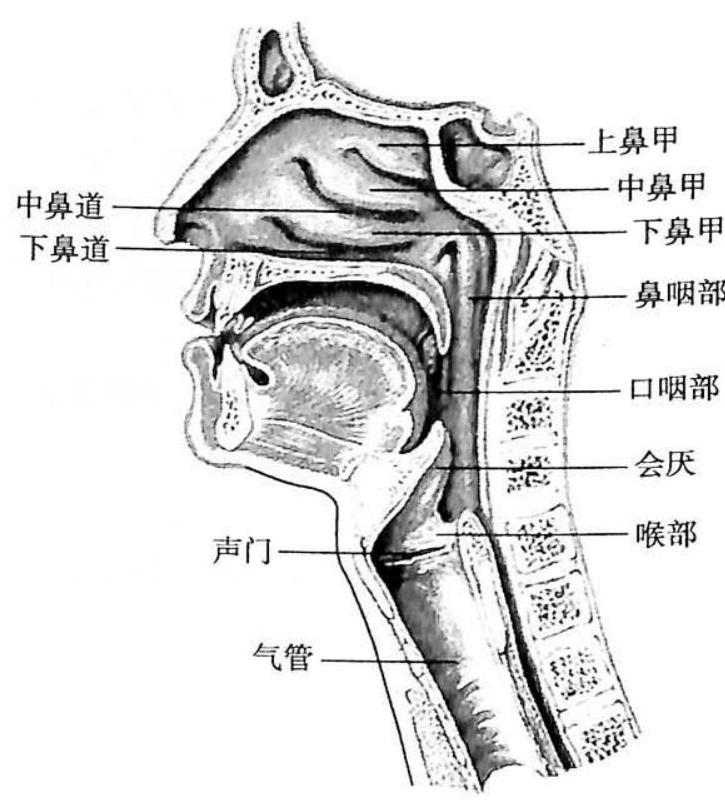
\includegraphics[max width=\textwidth]{2024_07_09_002a177993bd97d1d6d7g-083}
\end{center}

图 6-1 上呼吸道剖面示意图

\begin{enumerate}
  \item 领面及口部 领面部的解剖结构与面罩辅助通气时的气密性和气管内插管操作等有着密切的联系。张口度过小、下颌的退缩、颊部的消瘦凹陷以及突起的大鼻等都可能增加操作难度。口腔和牙齿的解剖异常也与插管困难密切相关, 如舌体过大、口腔内的增殖体或肿瘤、缺齿、残齿、门齿过长或前突、全口无牙等, 都可增加面罩通气和气管内插管的难度。

  \item 鼻 鼻是呼吸道的起始部分, 吸人的气体通常在这里被湿化和加温; 鼻毛和黏液还可起到过滤作用, 以阻挡空气中的粉尘和细小颗粒。平静呼吸时, $2 / 3$ 的气道阻力是气流通过鼻控时所产生的。经鼻呼吸时的气道阻力几乎是经口呼吸时的两倍, 这亦是剧烈运动时人类通常选择张口呼吸的重要原因。鼻腔顶部,尤其是鼻中隔前上区的黏膜,具有来自上领动脉分支极丰富的血管丛分布, 该区域亦称为鼻易出血区 (亦即 Little 区)。与置管损伤相关的鼻出血 $90 \%$ 以上都发生在该区域。经鼻置管时,严禁气管导管或胃肠引流管等进人上鼻道,以免造成难以控制的损伤和出血。鼻部气道梗阻的常见原因包括:鼻息肉、鼻中隔扭曲、炎症引起的䵑膜水肿和分泌物增加等。

  \item 咽 咽腔为呈漏斗状的肌性管道, 上接鼻后孔, 下至食管上端、梨状窝附近。以软腭下缘和会厌软骨上缘为界, 可将咽腔人为地区分为鼻咽腔、口咽腔和喉咽腔。鼻咽部和口咽部引起气道梗阻的主要原因分别是扁桃体肿大和颏舌肌松驰引起的舌后坠。

  \item 喉 喉位于第 3 颈椎至第 6 颈椎之间, 主要作用是发声和保护下气道。喉由肌肉、韧带\\
和软骨组成。软骨包括甲状软骨、环状软骨、会厌软骨以及三对成对的软骨 (杓状软骨、小角状软骨和楔状软骨), 其表面由䵗膜覆盖。喉部的肌肉非常活跃, 主要由迷走神经的分支支配。插管刺激或喉部的操作刺激可引起喉痉挛, 这也是气道梗阻的常见原因。

  \item 气管和主支气管 如图 6-2 所示,气管通常由 $12 \sim 20$ 个马蹄形软骨环组成,一般为 $15 \sim$ 16 个。成人气管长度为 $10 \sim 15 \mathrm{~cm}$, 平均约 $10.5 \mathrm{~cm}$ 。上部起始于环状软骨 (相当于第 6 颈椎水平),下部止于气管隆塍处(相当于第 4 胸椎下缘, 胸骨角水平), 向下气管分为左、右主支气管。气管和支气管黏膜表面有丰富的迷走神经纤维末梢分布,尤其是气管隆嘴部位,遇刺激后易引起剧烈的咳嫩和支气管㾤挛。引起气管和支气管梗阻的主要原因为: 气道分泌物或异物等阻塞、颈部巨大肿瘤侵犯或压迫以及严重支气管痉挛等。

\end{enumerate}

\begin{center}
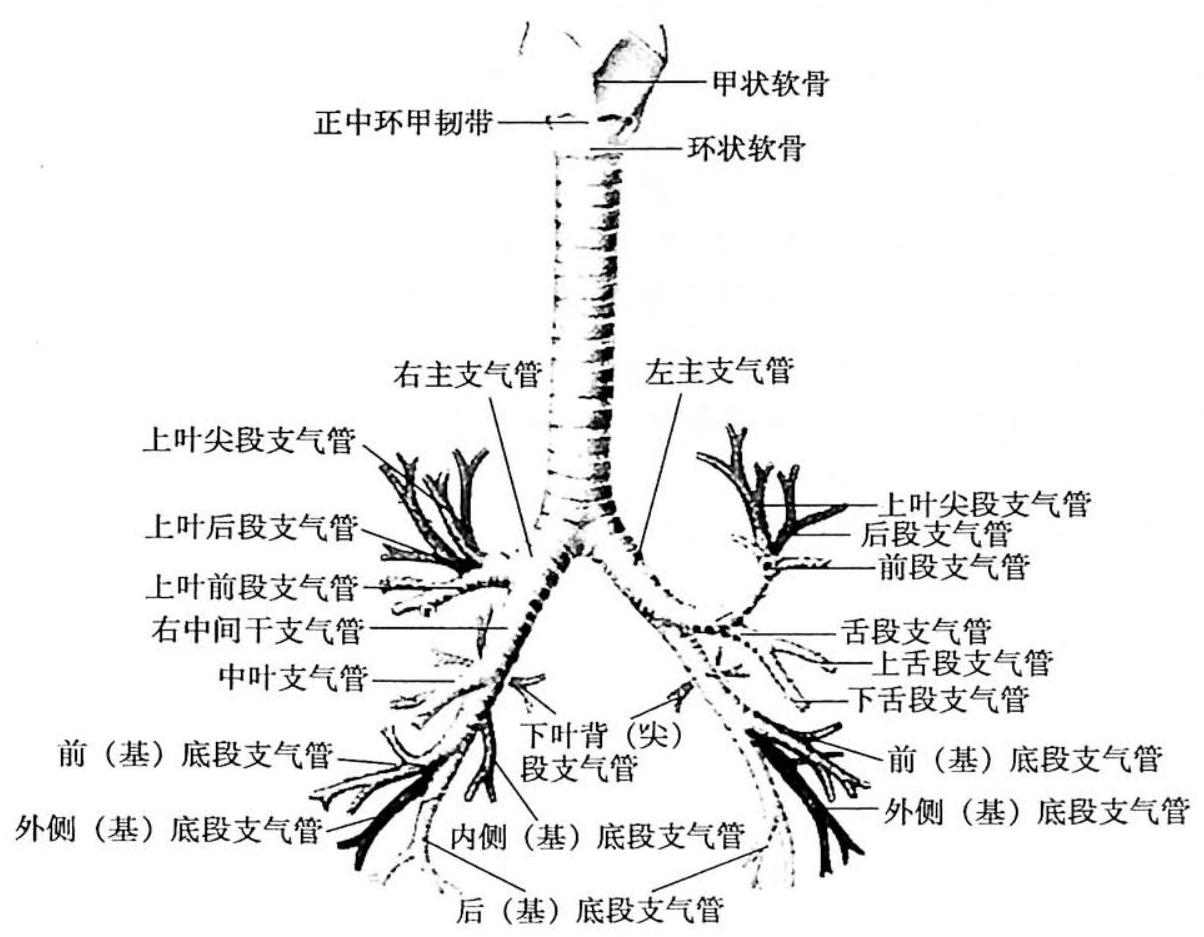
\includegraphics[max width=\textwidth]{2024_07_09_002a177993bd97d1d6d7g-084}
\end{center}

图 6-2 气管和支气管

\section*{二、影响解剖气道通畅的常见原因}
相对于气管导管等人工气道而言, 人体自身的气道属于解剖气道。临床上, 凡是能引起上至口咽部, 下至支气管等部位的气道狭窄或梗阻的因素, 都是影响解剖气道通畅的原因。常见原因有:

\begin{enumerate}
  \item 分泌物、出血和异物 分泌物、血液凝块以及异物阻塞是急诊患者气道梗阻的常见原因,在意识不清的患者中更容易出现。咽喉部分泌物多或有异物时, 常引起不完全性呼吸道阻塞,表现为吸气性呼吸困难, 听诊时可听到患者喉头部和(或)胸部有痰鸣音和高调的哮鸣音。
\end{enumerate}

处理原则: 尽快清除分泌物或异物。在气道通畅前, 应力争保留患者的咳嗽反射和自主呼吸,防止分泌物或异物向下呼吸道移行, 以致造成气道的完全性梗阻。分泌物过多或咽喉部有血液时, 应及时以负压吸引器吸除; 当异物或血凝块阻塞气道时, 可将患者舌头拉出, 用手或其他辅助器械将其清理干净; 当暴露或操作困难时, 可在直接喉镜下吸引或将异物取出, 以恢复气道通畅。

\begin{enumerate}
  \setcounter{enumi}{1}
  \item 舌后坠 是临床上气道梗阻最常见的原因,多发生于意识不清、全身麻醉诱导期与苏醒期患者以及非全身麻醉患者辅用镇静镇痛药时。患者仰卧位时, 在重力作用下下领骨和垓舌肌松驰,可造成舌体坠向咽后壁而阻塞气道。当舌后坠引起不完全性气道梗阻时, 最明显的表现\\
为随呼吸发出的强弱不等的萛声以及喉头拖曳征; 当舌后坠引起完全性气道梗阻时, 诅声消失,患者早期即出现明显的胸腹反常呼吸、三凹征和口鼻部的呼吸气流完全中断, 随即出现 $\mathrm{SpO}_{2}$ 进行性下降和发绀等,此时必须紧急处理。
\end{enumerate}

处理原则: 可采用单手抬下㬵法或双手托下领法, 或放置口咽或鼻咽通气管(详见本章第二节)。

\begin{enumerate}
  \setcounter{enumi}{2}
  \item 喉痉挛 喉痉挛是由于咽喉部应激性增高, 支配喉部的迷走神经兴奋性增加, 使声门关闭、活动增强所致。多发生在全麻诱导插管或术后苏醒拔管期, 特别是在浅麻醉或低氧和 $\mathrm{CO}_{2}$ 蓄积时, 进行喉部操作更容易诱发喉痉挛。临床表现为吸气性呼吸困难, 可伴有干咳及典型的高调吸气性喉鸣音。轻度喉痉挛仅假声带挛缩, 声门变窄, 吸气时出现喉鸣; 中度喉痉挛时, 真假声带均发生挛缩, 但声门未完全关闭, 吸气和呼气时都出现喉鸣音; 重度喉痉挛时, 声门紧闭, 呼吸道完全梗阻,呼吸音消失, $\mathrm{SpO}_{2}$ 迅速下降, 患者发绀。
\end{enumerate}

处理原则: 应强调以预防为主, 避免在低氧和 $\mathrm{CO}_{2}$ 蓄积或者浅麻醉下刺激喉部黍膜。轻度的喉痉挛一般在刺激解除后可自行缓解; 中度者需以面罩加压给氧,必要时以短效的麻醉药加深麻醉, 并辅助通气; 对于重度喉痉挛必须十分迅速地加深麻醉, 甚至可加用肌松药以解除痉挛,必要时行紧急气管内插管以解除梗阻; 当情况更危急或麻醉药物和器械不具备时, 可用粗针头等锐器紧急行环甲膜穿刺, 然后再准备行气管内插管或气管切开术。

\begin{enumerate}
  \setcounter{enumi}{3}
  \item 支气管痉挛 常因过敏、呕吐物反流误吸、分泌物过多, 以及气管内插管或异物刺激气管䵔膜而引起。临床表现以呼气性呼吸困难为特征, 患者的呼气期延长且费力, 听诊两肺满布哮鸣音, 常伴有窦性心动过速甚至更严重的心律失常。最严重的情况下, 患者肺部的呼吸气流完全中断, 听诊肺部哮鸣音反而消失, 出现 “寂静肺”。机械通气时, 最显著的特征为气道压显著升高,甚至难以通气。
\end{enumerate}

处理原则: 轻度支气管痉挛通过吸氧或以面罩加压给氧即可缓解。中重度时一般需用药物治疗, 如沙丁胺醇(舒喘宁) 或异丙托溑铵 (爱全乐)气雾剂吸人、静脉注射或雾化吸人糖皮质激素等。围术期出现急性支气管痉挛者, 往往为有哮喘病史或气道高反应性的患者, 麻醉过浅是最常见的诱因, 因此, 及时加深麻醉常能起到事半功倍的效果。

\begin{enumerate}
  \setcounter{enumi}{4}
  \item 药物残余作用所致通气障碍 除了神经肌肉系统的病变可导致限制性通气功能障碍外,能抑制中枢神经系统的麻醉药以及肌松药的应用过量、蓄积或残余作用等, 也可造成患者的通气功能障碍, 表现为低氧血症和高碳酸血症。
\end{enumerate}

处理原则: 轻者可应用简易呼吸器或麻醉机面罩辅助呼吸, 重者宜气管内插管辅助/控制呼吸。同时, 可针对性地应用麻醉药和肌松药的特异性拈抗剂, 如氟马西尼、纳洛酮和新斯的明等。

\section*{第二节 维持气道通畅的方法}
目前已有多种方法可用于控制气道。针对患者的不同情况, 在选择何种方法控制气道时,所遵循的基本原则是:选择最简便、有效、安全而又被操作者所熟悉的方法。临床上,除了全麻患者气管内插管是在手术室内实施以外, 多数需紧急气道处理的患者都位于手术室外, 难以在数分钟内紧急呼叫麻醉科医师到场处理气道。这时, 如果临床医师被动地等待专业医师来建立人工气道, 往往使患者丧失了宝贵的救治时机。此时,一些简单的清理气道、手法辅助通气以及简便的人工气道建立方法, 常常可以发挥难以估量的作用。

\section*{一、维持气道通畅的基本方法}
\section*{(一)单手抬下放法和双手托下领法}
这两种手法是解除因舌后坠所致上呼吸道机械性梗阻最简便有效的方法, 也是各临床工作\\
者均需掌握的基本方法。

\begin{enumerate}
  \item 单手抬下㬵法 如图 6-3A 所示, 患者取仰卧位, 操作者将患者的头后仰, 以一只手在下垓部向患者的上方抬举下颏, 力争将患者的舌体抬离咽后壁, 从而解除舌后坠造成的气道梗阻。此方法在临床使用时的局限性较多。当患者存在头颈部粗短、肥胖、鼻道阻塞、牙关紧闭、颈部强直等情况时, 往往难以奏效。此时需考虑采用双手托下颌法或其他方法。

  \item 双手托下领法 如图 6-3B 所示, 患者取仰卧位, 操作者立于患者的头端, 将患者的头略后仰, 双手的示指或中指置于患者下领角的后支, 向前、上方托举下领。为了有效地将患者的舌体抬离咽后壁,应尽量使患者下门齿的高度超过上门齿(俗称为“地包天”)。\\
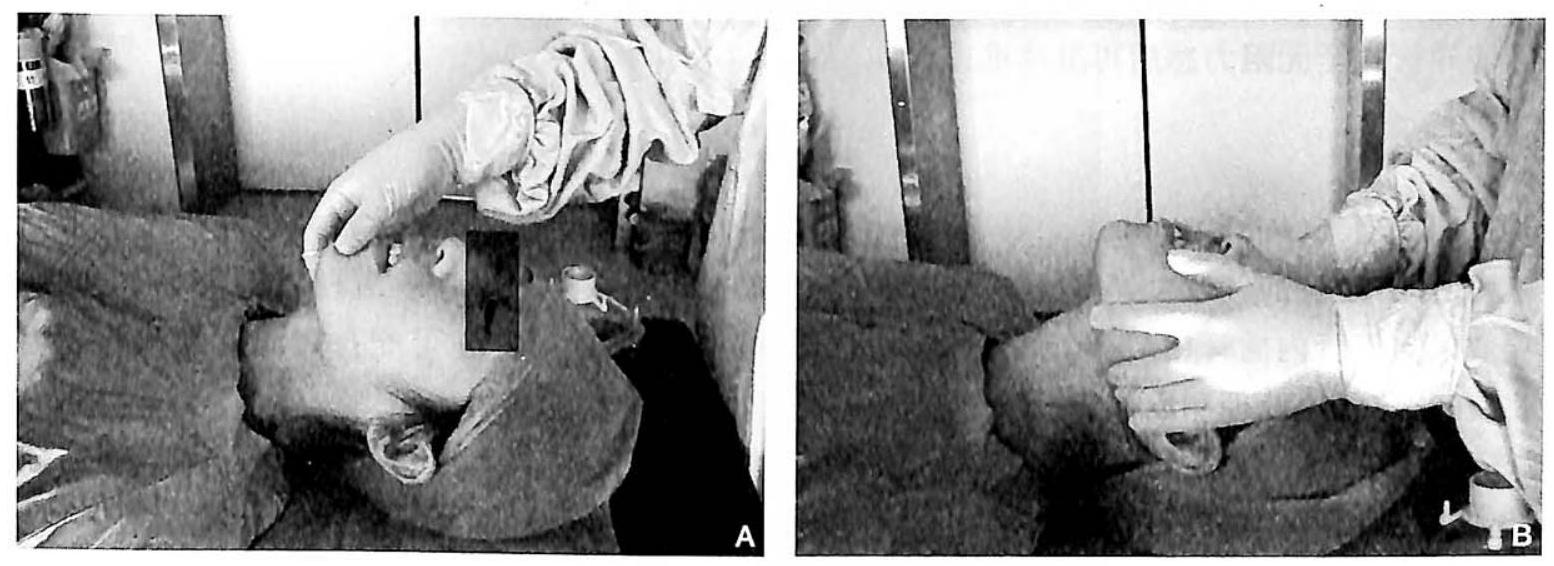
\includegraphics[max width=\textwidth, center]{2024_07_09_002a177993bd97d1d6d7g-086(1)}

\end{enumerate}

图 6-3 手法维持气道通畅

A. 单手抬下㬵法; B. 双手托下领法

\section*{(二) 口咽、鼻咽通气管的使用}
如需较长时间解除梗阻或手法托举无效时, 可放置口咽通气管或鼻咽通气管, 以帮助开放气道。

\begin{enumerate}
  \item 口咽通气管 (oropharyngeal airway) 是用金属、硬橡胶或硬塑料制成的、外观略呈 J 形、中空的人工气道(图 6-4)。
\end{enumerate}

\begin{center}
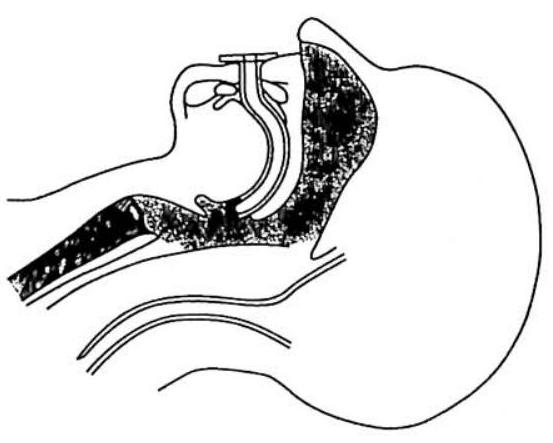
\includegraphics[max width=\textwidth]{2024_07_09_002a177993bd97d1d6d7g-086}
\end{center}

图 6-4 放置口咽通气管

操作方法: 依据患者的体型选择适当大小的通气管。向患者头侧方向将通气管的前端 (其凹面朝向头端) 插人口腔, 然后一边旋转通气管 $180^{\circ}$ 、一边推进通气管直至咽腔。此方法可避免在推送通气管的过程中将舌体推向口腔深部,造成置管困难。也可利用压舌板或喉镜片压迫舌体后,将通气管放人口咽部。此时口咽通气管的弯曲弧线恰好与患者舌体的自然弧度贴合。

注意事项: (1)清醒或浅麻醉患者使用口咽通气管时,可出现恶心呕吐、呛咳、喉痉挛和支气管痉挛等反射, 因此只适用于非清醒或麻醉深度恰当的患者; (2)通气管位置放置不恰当时, 反而会将舌根推至咽腔深部而加重梗阻或引起喉痉挛、舌及咽部损伤等; (3)如患者不能开口, 又不宜使用鼻咽通气管时, 可先将两个压舌板分别置人双侧上下后臼齿之间, 利用杜杆作用援开口腔, 再置人口咽通气管。

\begin{enumerate}
  \setcounter{enumi}{1}
  \item 鼻咽通气管 (nasopharyngeal airway) 是用橡胶或塑料等制成的软质中空导管,长度约 $15 \mathrm{~cm}$, 外形与气管导管相似。其前端斜口较短而钝圆, 不带套露。主要用于解除舌后㓌等所致的上呼吸道梗阻,尤其是咬肌痉挛的患者(图 6-5)。由于患者对其耐受性好,较少发生恶心、呕\\
吐和喉疼挛。由于通气管是由患者的鼻孔插人, 且管径较大,易致出血, 因此, 对于凝血功能异常、顾底骨折、鼻咽腔感染或鼻中隔外伤移位等患者禁忌使用。
\end{enumerate}

操作方法: (1)选择通畅的一侧鼻孔置人。插人前在鼻腔内滴人适量血管收缩药, 如麻黄碱等, 以减少鼻腔出血的风险。(2)先于通气管表面涂以含局部麻醉药的医用润滑剂 (导管胶)。(3)通气管的插人长度一般为鼻尖至外耳道的距离,这样通气管前端恰好位于会厌的上方。(4)通气管必须沿下鼻道插人,保持插人方向与面部完全垂直,严禁指向鼻

\begin{center}
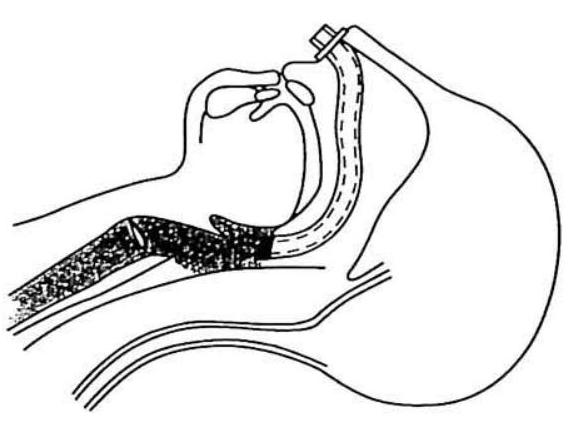
\includegraphics[max width=\textwidth]{2024_07_09_002a177993bd97d1d6d7g-087}
\end{center}

图 6-5 放置鼻咽通气管顶部方向插人, 以免造成损伤出血。(5)插人动作应轻柔、缓慢, 遇有阻力不应强行插人, 可稍稍旋转导管直至无阻力感后再继续推进。

\section*{二、面罩通气}
面罩通气(mask ventilation)技术是各级临床医师必须掌握的一项基本技能。其设备要求简单、操作方便且通气效果确切, 且可提供较高浓度的氧疗; 在无明显呼吸道梗阻的情况下, 其通气效果与气管内插管相似; 患者的耐受性良好, 不需要较深的麻醉亦可配合完成通气操作。因此,在紧急气道处理和危重病救治中,至今仍发挥着不可替代的作用。

\begin{enumerate}
  \item 适应证 (1)为无胃内容物反流、误吸危险者的短小手术施行全身麻醉通气; (2)气管内插管前为患者预充氧去氮; (3)紧急情况下进行辅助或控制呼吸,如心肺复苏的现场急救。
\end{enumerate}

\section*{2. 操作方法}
(1) 物品的准备: 选择大小合适的透明通气面罩, 以使面罩能紧贴鼻梁、面颊和口, 并可观察到口唇颜色和分泌物情况。检查贮气球蘦, 使之与供氧管相连接, 并确保无漏气。应备有适当的口咽通气管、鼻咽通气管, 以及负压吸引装置等。

(2) 面罩的放置:单人操作时, 操作者左手持面罩, 用小指提起下领角, 中指与无名指置于下领骨处, 示指与拇指置于面罩上, 适当用力以保持面罩的气密性; 右手控制发气球起行手法通气(图 6-6A)。如患者头面部较大、面罩难以密闭时, 则可能需要双人操作。这时, 操作者双手维持面罩于良好的位置,助手控制发气球覀( 图 6-6B、C)。也可使用四头带帮助将面罩固定于患者的面部。要求既要保证面罩与患者面部的紧密贴合、无明显漏气, 又要能通过托举下领角的动作解除舌后坠造成的气道梗阻。

(3) 辅助或控制呼吸的操作要点:在操作者用右手或由助手行辅助或控制呼吸时, 应通过观察或手感来判断患者胸廓起伏的幅度和通气阻力的大小, 并评估通气效果。可通过使患者头部略后仰、抬起㬵部或托起下领的方法, 使患者下领骨向前上抬起并张口, 来改善通气效果 (图 6-6)。必要时可置人口咽或鼻咽通气管。吹人一次潮气量 $(6 \sim 8 \mathrm{ml} / \mathrm{kg})$ 的时间一般不少于 1 秒。缓慢而均匀地供气可最大限度地避免胃膨胀的发生。

\begin{enumerate}
  \setcounter{enumi}{2}
  \item 注意事项 由于在进行面罩通气时, 并没有将人工气道与下呼吸道紧密连接, 因而使用时需要注意:
\end{enumerate}

(1)必须彻底清除气道内的分泌物、血液和异物等, 否则在正压通气下, 有加重气道梗阻的风险。

(2)面罩通气时,气体有进人胃肠道的风险,使患者发生反流误吸的风险增加。

(3) 对于下呼吸道梗阻, 面罩通气往往效果差或无效。

\begin{enumerate}
  \setcounter{enumi}{3}
  \item 常见并发症 较长时间面罩通气引起的口、眼或鼻周围软组织压伤最为常见, 而胃内容物反流误吸是其最严重的并发症。保持患者镇静和(或)配合、控制通气压力和潮气量等是防止反流误吸最有效的措施。\\
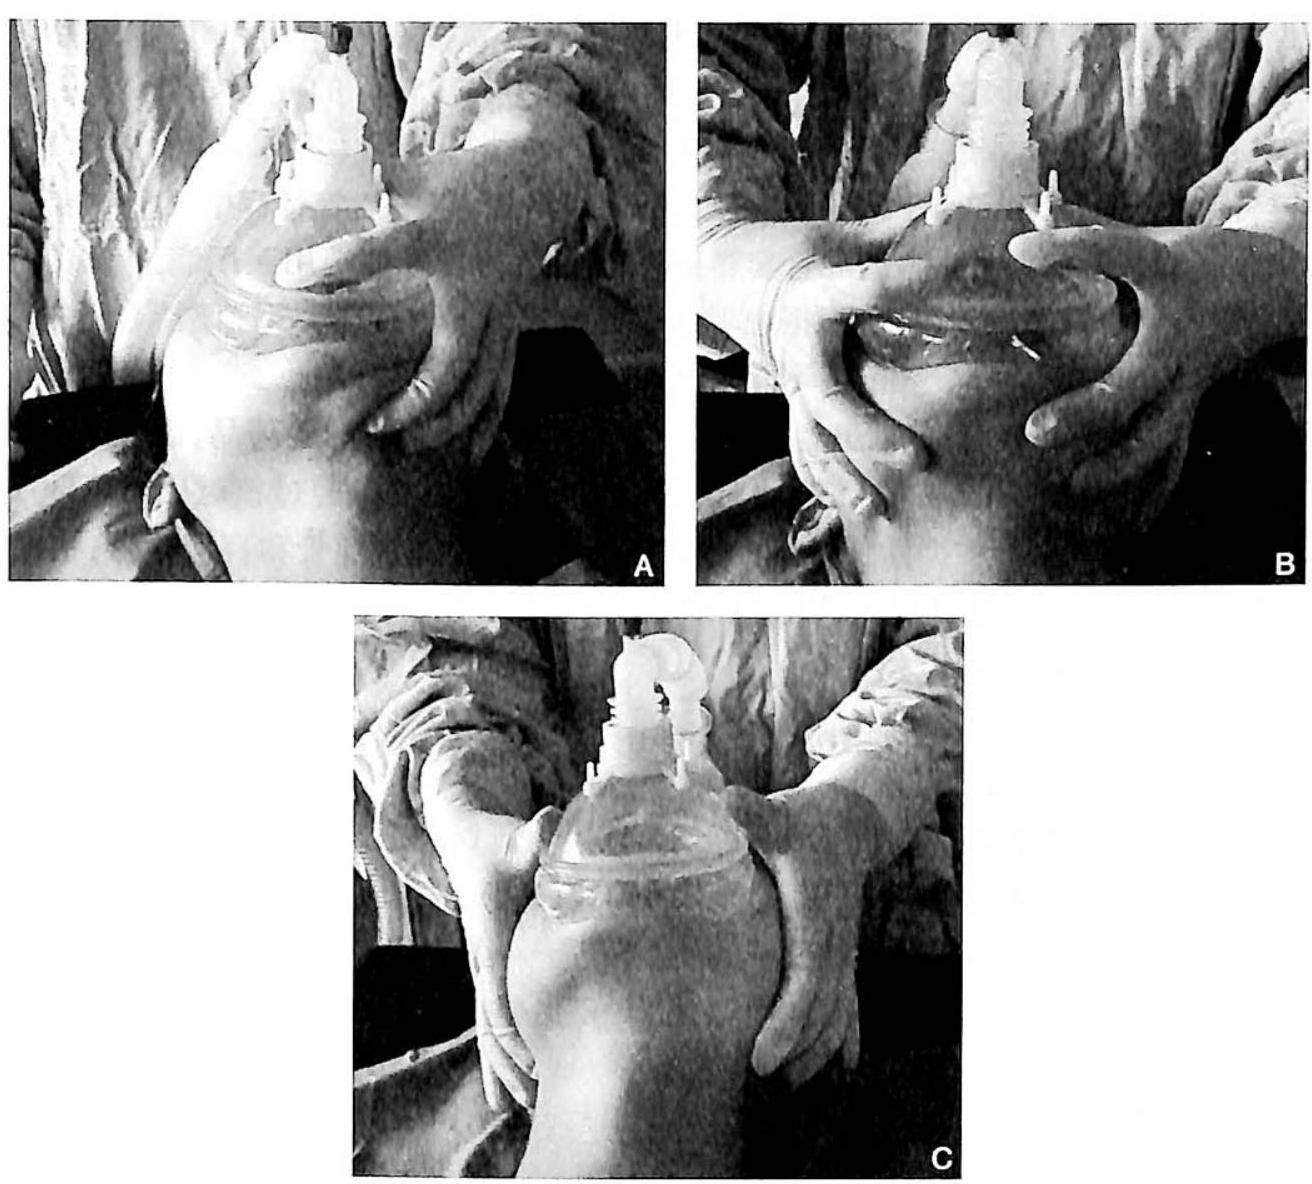
\includegraphics[max width=\textwidth, center]{2024_07_09_002a177993bd97d1d6d7g-088}
\end{enumerate}

图 6-6 面罩通气的手法

\section*{三、气管插管术}
气管插管术通常又可分为气管内插管 (endotracheal intubation)和支气管内插管 (broncheal intubation)两类。气管内插管是将人工气道与解剖气道连接的最可靠的方法, 也是麻醉科医师和急诊医师 (包括 ICU 医师)所必须掌握的基本技能之一。

\section*{(一)气管内插管}
\begin{enumerate}
  \item 适应证 气管内插管可保持患者的呼吸道通畅, 防止异物进人呼吸道, 便于及时吸出气管内分泌物或血液; 进行有效的人工或机械通气; 便于吸人全身麻醉药的应用。因此, 凡是在全身麻醉时, 难以保证患者呼吸道通畅者(如顾内手术、开胸手术、俯卧位手术等), 因疾病难以保持呼吸道通畅者(如肿痹压迫气管), 全麻药对呼吸有明显抑制或应用肌松药者,都应行气管内插管。因各种原因需要进行机械通气者、心肺复苏以及新生儿严重窒息时, 都是气管内插管的适应证。

  \item 插管前准备 插管前必须做到所有设备和器材就位且功能正常, 人员到位, 相关药品 (麻醉药、血管活性药等) 准备到位。插管前准备不足或对困难气道预计不够, 不仅可导致插管失败, 更可能威胁患者的生命安全。常用器械包括:喉镜、气管导管、牙垫或口塞、表面麻醉用喷雾器, 衔接管、管芯、插管钳、固定胶带以及负压吸引装置等。

\end{enumerate}

(1)插管前对患者的检查和评估: 插管前应常规对患者进行有关检查和评估, 并了解气管内插管的难易程度。患者既往的手术麻醉史对判断插管的难易度有重要参考价值。

(2)喉镜的选择和检查: 临床上可供选择的直接喉镜种类较多,其用途和使用方法也各不相同,应根据操作者使用习惯及患者情况加以选择。目前最常用的仍是最传统的 Macintosh 喉镜( 弯喉镜片)。成人气管内插管多选择3 号或 4 号 Macintosh 喉镜。使用前须检查喉镜电池的\\
电量是否充足、喉镜片前端的灯泡或光纤是否明亮。

(3) 气管导管的选择和检查:成人一般选择内径 $7.0 \sim 7.5 \mathrm{~mm}$ 的气管导管, 小儿气管导管内径 $(\mathrm{mm})$ 可根据经验公式进行选择, 即导管内径 $(\mathrm{mm})=$ 患儿年龄 $($ 岁 $) / 4+4$ 。选择好导管后,应另外再备两根分别大于和小于该导管内径 $0.5 \mathrm{~mm}$ 的导管, 以备插管过程中根据患者的实际情况及时调整气管导管的型号。检查导管套䓡是否漏气,并将导管前端用医用润滑剂或生理盐水润滑; 将导管芯置于气管导管腔内, 根据患者的喉部位置情况, 将气管导管保持合适的弯曲度,以便提高插管的成功率。导管芯前端不能超出气管导管。

(4)药品的准备和核对: 根据患者的病情,选择和准备合适的麻醉药品, 以及辅助用药,包括镇静催眠药、麻醉性镇痛药和肌松药等。麻醉期间所用药品,必须经过核对后方可使用。

\begin{enumerate}
  \setcounter{enumi}{2}
  \item 气管内插管方法 根据插管时是否需要显露声门分为明视插管和盲探插管; 根据插管路径分为经口插管和经鼻插管; 根据插管前麻醉方法分为慢诱导插管 、快诱导插管和清醒插管等。
\end{enumerate}

(1) 经口明视气管内插管术

1)预充氧去氮:患者插管前以面罩吸纯氧至少 3 分钟, 以排出患者体内的氮气,增加肺内的氧气储备, 延长插管的安全时限。

\begin{enumerate}
  \setcounter{enumi}{1}
  \item 插管的体位:自患者的口腔至气管之间可以人为地划出三条解剖轴线: 口轴线为口腔至咽后壁的轴线 $(\mathrm{OA})$ 、咽轴线为咽后壁至喉头的轴线 (PA) 、喉轴线为喉腔至气管上段的轴线 (LA)。患者仰卧时, 这三轴线彼此相交成角,并不处于一条直线。如果在患者枕下垫一薄枕,使患者的头部垫高约 $10 \mathrm{~cm}$, 并头后仰( “嗅花位”), 可以使患者咽、口、喉三轴线接近重叠, 插管径路接近为一条直线, 利于显露声门(图 6-7)。
\end{enumerate}

\begin{center}
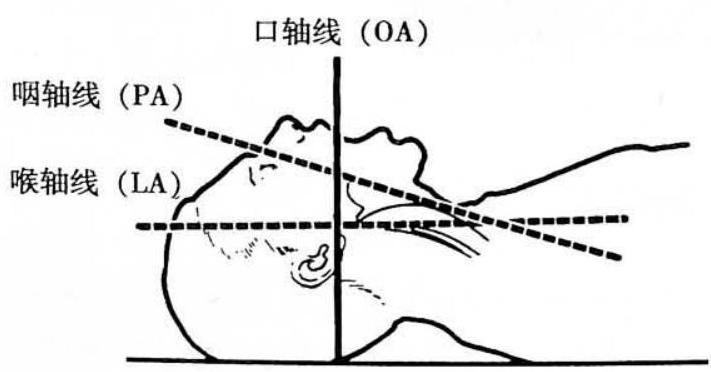
\includegraphics[max width=\textwidth]{2024_07_09_002a177993bd97d1d6d7g-089}
\end{center}

A\\
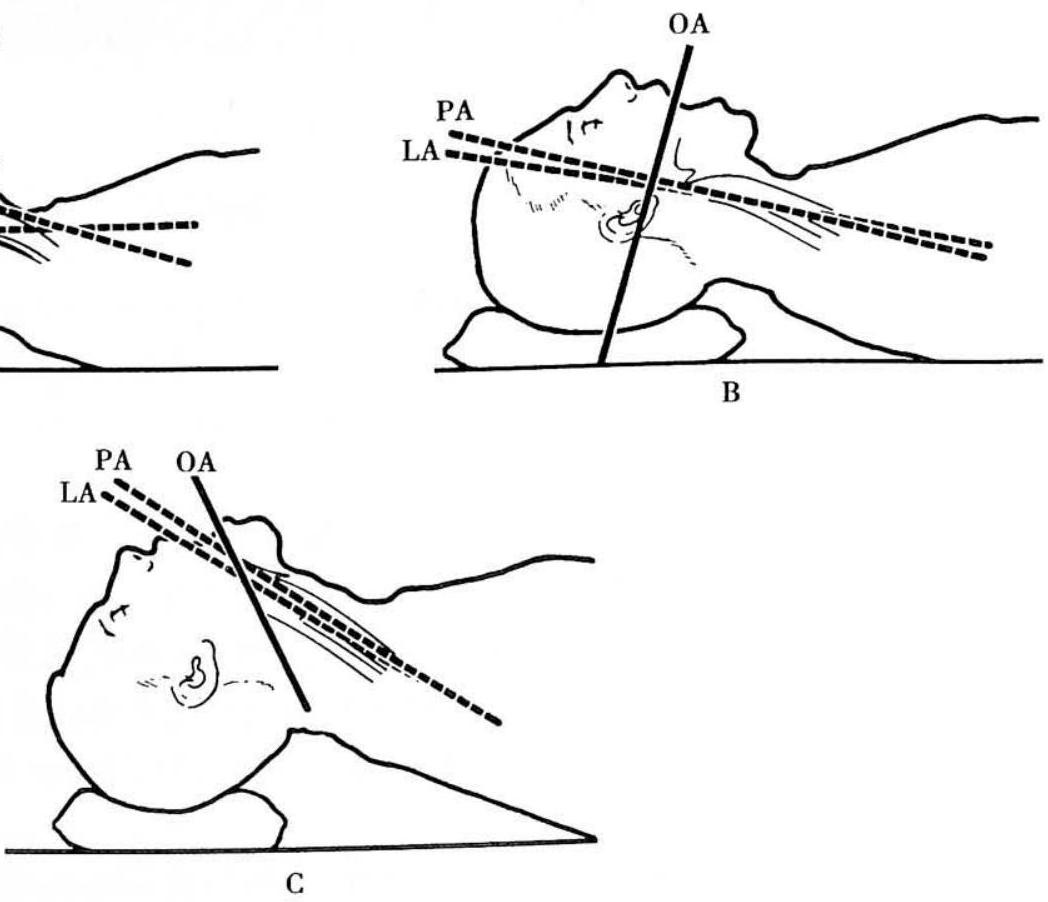
\includegraphics[max width=\textwidth, center]{2024_07_09_002a177993bd97d1d6d7g-089(1)}

图 6-7 气管内插管时头部位置示意图

A. 平卧位时,三轴线相互成角;B. 枕下垫高约 $10 \mathrm{~cm}$ 后, PA 与 LA 接近重叠,但仍与 OA 明显成角;

C. 枕下垫高约 $10 \mathrm{~cm}$ 、头后仰(“嗅花位”)时,三轴线的成角变小,接近重叠,便于喉镜显露声门

\begin{enumerate}
  \setcounter{enumi}{2}
  \item 插管操作方法: 操作者左手持喉镜柄, 右手提颏张口并拨开上下唇。从患者右侧口角置人喉镜片, 边沿患者的舌背面向下滑行, 在将喉镜片逐渐移至口正中部的同时, 将舌体略压向左侧。显露悬雍垂后, 继续沿舌背部的曲线轻箱地将喉镜片向下滑人, 直至看见会厌软骨。使用弯喉镜片时, 在明视下将喉镜片的前端伸人舌根与会厌软骨根部之间的会厌谷, 再向上、略向前
\end{enumerate}

\begin{center}
\includegraphics[max width=\textwidth]{2024_07_09_002a177993bd97d1d6d7g-090(3)}
\end{center}

A

\begin{center}
\includegraphics[max width=\textwidth]{2024_07_09_002a177993bd97d1d6d7g-090(2)}
\end{center}

C

\begin{center}
\includegraphics[max width=\textwidth]{2024_07_09_002a177993bd97d1d6d7g-090(1)}
\end{center}

B

\begin{center}
\includegraphics[max width=\textwidth]{2024_07_09_002a177993bd97d1d6d7g-090}
\end{center}

图 6-8 Macintosh喉镜(弯喉镜片) 操作示意图

方上提喉镜, 使会厌向上翅起紧贴喉镜片, 以显露声门 (图 6-8)。如果使用直喉镜片 (如 Miller 喉镜) 时, 在暴露会厌软骨后, 将镜片置于会厌软骨的喉面, 直接向前上方挑起会厌, 即可显露声门。注意上提喉镜时, 用力的方向应与喉镜柄的方向一致,即朝向患者脚部上方天花板的方向,大致为前上方 $45^{\circ}$ 。这时注意不要弯曲自己的腕部或将喉镜片在患者的牙齿上琵动, 以免损伤牙齿或软组织。

置管时右手以持笔式持气管导管, 在明视声门的情况下将气管导管沿患者的右口角置人,避免导管阻挡操作者的视野,亦不要使牙齿刮破导管套䗱。气管导管进人声门后, 将导管内的导管芯拔出, 继续置管, 直到气管导管的套蓌进人声带下 $3 \sim 4 \mathrm{~cm}$ 的位置。然后将牙垫置人患者的门齿之间, 退出喉镜。使用注射器将导管套垩充气, 最佳充气标准是使套露内压力为手控呼吸下套露周围无漏气时的最小压力。成年人置管平均深度 (即气管导管前端至门齿距离) 为 $18 \sim 22 \mathrm{~cm}$ 。

4)气管导管位置的判定: 理想的导管位置其前端应位于气管的中段, 气管隆塍上 $3 \sim 7 \mathrm{~cm}$ 。确认气管导管位置的常用方法包括: (1)将气管导管与 $\mathrm{CO}_{2}$ 探测器或呼气末 $\mathrm{CO}_{2}$ 监测相连, 行数次人工通气, 以检测气道内出现的 $\mathrm{CO}_{2}$; 出现正常的 $\mathrm{P}_{\mathrm{ET}} \mathrm{CO}_{2}$ 波形是气管导管位于气管内的可靠指标。(2)以听诊器依次置于患者两侧的胸前区及腋中线, 听诊并观察正压通气时双肺的呼吸音和胸廓起伏幅度是否一致。插管后若患者一侧肺呼吸音消失, 提示导管可能过深而进人了另一侧主支气管, 需要缓慢地退管, 直到双肺呼吸音对称。(3)若条件允许, 可以胸片来判断导管的位置。要确保导管上的标志线前端位于气管中部, 而没有进人一侧支气管。但该方法并不能可靠地判断导管是否位于食管内。

5)气管导管的固定: 最好采用专用的导管固定器来固定导管; 也可采用胶带或气管导管固定带固定导管。ICU 患者插管后应用适当的镇静药物, 并限制患者上肢的活动, 以防患者自己意外拔管。

6)注意事项:(1)插管时患者应处于适当的麻醉深度, 以使咬肌松弛、张口满意, 并抑制咽喉反射; (2)暴露过程中如发现咽喉反射活跃, 宜暂停插管, 在辅助通气下适当加深麻醉; 清醒插管\\
者可作喉部表面麻醉; (3)喉镜的着力点应始终位于喉镜片的顶端, 并采用上提喉镜的手法, 严禁将上门齿作为支点,以防损伤牙齿; (4)导管插人声门时必须动作轻柔, 避免使用暴力。

(2) 经鼻气管内插管术

1)适应证: 与经口明视气管内插管相似。尤其适于一些不适合经口明视气管内插管的特殊患者选用,如颈椎不稳、下领骨骨折、口咽部感染、需较长时间带管者等。

2)禁忌证:此操作的创伤程度高于经口明视气管内插管。主要禁忌用于凝血功能障碍、面部中段创伤、颎底骨折以及可能有颅内压升高等患者。

3)操作要点:经鼻气管内插管包括经鼻明视法和盲探法两种。

经鼻明视气管内插管时, 喉镜的操作要领与经口明视气管内插管相似。选择通气较好的一侧鼻孔插管。气管导管应使用医用润滑剂充分润滑,鼻腔内施行表面麻醉, 并滴人数滴 $3 \%$ 麻黄碱以使鼻腔黏膜血管收缩, 减少出血风险。置管时注意气管导管应与面部垂直置人冝孔, 沿下鼻道插管, 以免出现损伤和难以控制的出血。导管难以进人声门时, 可采用插管钳辅助置管。

经鼻盲探气管内插管是在保留患者自主呼吸的情况下, 导管置人鼻腔后, 通过患者呼吸气流的导引而盲探置管的一种方法, 既往多用于喉镜暴露困难或不适于喉镜暴露而需气管内插管的患者。该方法要求操作者具备丰富的插管经验, 成功率也难以保障, 并不适合初学者使用。近年来,随着纤维支气管镜等辅助插管技术日益成熟和推广, 该方法在临床上的使用日渐减少。

\section*{(二)支气管内插管}
支气管内插管是将支气管导管置人气管隆塍以下的支气管内, 以建立单肺或双肺分别人工通气的方法。其目的是将两侧肺隔开分别通气,并可分别吸除双侧肺内的分泌物。主要用于咯血患者、肺脓肿或罼肿患者、其他肺部或食管手术以及支气管肺泡灌洗等患者,以保护非手术侧肺功能或提高胸腔内手术野的显露质量。

支气管内插管需要特制的支气管导管。支气管导管主要有两种: 双腔支气管导管 (分为左侧管和右侧管) 和 Univent 导管。双腔支气管导管型号包括 $28 \sim 41 \mathrm{~F}$ (一般成年男性为 $39 \sim 41 \mathrm{~F}$,女性为 $35 \sim 37 \mathrm{~F}$ ), 每一型号均有专门用于左侧或右侧的双腔支气管导管。多数情况下使用左侧双腔支气管导管即可完成手术,以降低右上叶支气管被导管阻塞的风险。但有不少学者主张选择非手术侧双腔支气管导管, 这可保证导管不会妨碍需行主支气管切除的手术操作, 也可避免手术操作牵拉肺门而影响支气管导管的位置。

\section*{(三)气管内插管的常见并发症}
\begin{enumerate}
  \item 气管内插管所引起的创伤 气管内插管可能造成口唇、舌、牙齿、咽喉或气管黍膜的损伤, 偶可引起环杓关节脱位或声带损伤。只要细心操作, 避免暴力, 一般不会发生或症状轻微。

  \item 气管导管不畅 气管导管扭曲、导管气並充气过多阻塞导管开口、俯卧位时头部扭曲、头过度后仰等体位使导管前端斜开口处贴向气管壁,以及导管衔接处内径过细等多种原因, 均可能导致气道不全或完全阻塞。此时应根据原因做好预防。一旦发生, 经处理仍不能解除时, 可用纤维支气管镜检查以明确原因, 并给予相应处理, 或立即更换气管内导管。

  \item 痰液过多或痰研痰液过多或痰痻阻塞气管导管常见于小儿或长时间留置导管的患者。对于长时间留置导管的患者要定期吸痰, 并且进行气道湿化, 以防痰痢形成。在充气套露上方的气管与导管之间的缝陌内可存留较多的分泌物或痰液, 一旦套霮放气, 即可能流人气道内引起气道梗阻,所以要定期清理干净。

  \item 气管导管插入过深阻塞一侧支气管 气管导管插人过深容易误人一侧支气管而使另一侧支气管无通气, 特别是在插管后头部位置变动, 以及腹腔镜气腹手术引起膈肌和气管上抬时易发生。最好的诊断方法是听诊两肺呼吸音和观察两侧胸部呼吸动度。一旦发生应及时调整好气管导管的位置。

  \item 麻醉机或呼吸机故障 麻醉机或呼吸机活瓣失灵、管道脱落、呼吸机湿化水在管道内凝\\
结过多阻塞气道以及其他机械因素均可引起气道阻塞。及时发现并处理非常重要, 必要时更换麻醉机或呼吸机。

\end{enumerate}

\section*{四、气管切开术}
气管切开术 ( tracheostomy) 是通过切开颈段气管开放下呼吸道, 并可置人金属或硅胶气管切开套管, 以解除上呼吸道梗阻。这是建立通畅人工气道的一种常见手术操作, 是临床医师应掌握的急救技能之一,尤其是麻醉与危重病医学专业医师。

目前, 除传统的气管切开术外, 可供选择的气管切开方法, 还包括环甲膜穿刺术、环甲膜切开术和经皮扩张气管切开术 (percutaneous dilational tracheostomy,PDT)。其主要适应证包括: (1)各种原因所致的急性上呼吸道梗阻, 如急性喉炎、严重喉痉挛和上呼吸道异物阻塞等; (2) 口腔领面部严重外伤, 无法行气管内插管者; (3)各种原因所致的气管内插管失败, 尤其是出现非预见性的困难气道时; (4)下呼吸道痰液或分泌物渚留或阻塞, 为便于及时清理气道、维持下呼吸道通畅时;(5)需较长时间保持人工气道和机械通气等。

气管切开术常见的并发症主要包括: 皮下气肿、气胸、纵隔气肿、出血、气道梗阻、喉部神经损伤、食管损伤甚至气管食管瘘、声带损伤、声门下狭窄以及气管狭窄等。

\section*{(一)常规气管切开术}
\begin{enumerate}
  \item 术前准备 除需准备制式的气管切开包外, 还应准备好氧气、负压吸引器、气管切开套管、简易呼吸皮露或呼吸机以及各种急救药品等。对于非紧急气管切开的患者,可考虑先行气管内插管和氧疗, 待呼吸困难缓解后, 再行气管切开术。

  \item 体位一般取仰卧位, 肩颈部适当垫高, 使头后仰、气管尽量接近皮肤, 便于手术的暴露和操作。颈部常规消毒、铺单或洞巾。

  \item 麻醉 对于全麻状态下或严重意识障碍的患者,可不必麻醉。其他多选用局部浸润麻醉,阻滞范围上自甲状软骨下缘,下至胸骨上窝。

  \item 操作方法 一般为双人操作, 作颈部正中直切口, 自甲状软骨下缘至接近胸骨上窝处切开皮肤及皮下组织。以血管钳沿正中线钝性分离胸骨舌骨肌和胸骨甲状肌,暴露出甲状腺峡部。向上牵引甲状腺峡部, 或切断并缝扎峡部, 以暴露出气管环。一般于第 $2 \sim 4$ 气管环处用尖刀片自下向上切开两个气管环;以弯血管钳撑开气管切口,置人适当大小的气管切开套管;拔出管芯, 吸净术野及气管内的血液和分泌物, 并检查无明显出血。将气管切开套管与呼吸机连接行机械通气或维持开放气道自主呼吸。以套管上的系带环绕颈部将切开套管固定, 注意避免固定过紧或过松,以免压迫颈部血管或切开套管意外脱出。皮肤切口一般不需缝合, 以无菌纱布垫覆盖于皮肤切口与套管之间即可。

\end{enumerate}

\section*{(二)环甲膜穿刺术}
该方法是仅在急性严重上呼吸道梗阻情况下采取的急救措施。一般尽量选用大口径的静脉套管针或金属针头, 经环甲膜穿刺。穿刺时,针体与患者皮肤成 $30^{\circ}$ 角,针尖指向患者足端, 当感觉到明显落空感、回抽有空气时, 表明针尖进人气管, 即可退出针芯将套管针留在气管内。通过套管针可进行高频喷射通气或接麻醉机行小潮气量手法快速通气。该方法只能作为困难气道的紧急处理措施, 应同时准备和尽快施行常规气管切开或气管内插管。

\section*{(三)环甲膜切开术}
与环甲膜穿刺术相似, 环甲膜切开术通常也是作为一种解除上呼吸道梗阻的紧急措施, 应同时准备和尽快进行常规气管切开或气管内插管。操作时尽量将患者置于与常规气管切开术相同的体位, 于甲状软骨和环状软骨间作一长约 $2 \sim 4 \mathrm{~cm}$ 的皮肤横切口, 于接近环状软骨处切开环甲膜, 以弯血管针撑大切口。此时即可解除上呼吸道梗阻, 经环甲膜切口置人适当大小的气管切开套管或气管导管,与呼吸机或麻醉机连接可行机械通气。

\section*{(四)经皮扩张气管切开术}
目前国内大多数医院中, 传统的气管切开术仍需要专科医师 (如耳鼻喉科医师) 进行, 且需要特殊的手术器械和导管, 从而极大地限制了其在紧急困难气道处理中的应用。为了适应麻醉与重症医学发展的需要, 近十余年来, 已研制了多种可供临床选择的微创经皮扩张气管切开套件。图 6-9 为经皮扩张气管切开套件的基本组成。

\begin{center}
\includegraphics[max width=\textwidth]{2024_07_09_002a177993bd97d1d6d7g-093}
\end{center}

图 6-9 经皮扩张气管切开套件

A. 穿刺套管针与注射器; B. 导引钢丝;C F. 不同管径的扩张器, 依次从小到大;G. 气管切开套管

操作方法 取颈前正中第 $1 \sim 2$ 或第 $2 \sim 3$ 气管环间陌处作一长约 $1 \mathrm{~cm}$ 的皮肤横切口; 以穿刺套管针在切口正中垂直向下穿刺人气管内; 当穿刺针有明显落空感且注射器回抽见空气后,退出针芯并经套管针置人导引钢丝至气管内; 退出套管针并将导引钢丝留在气管内; 使用不同管径的扩张器经导引钢丝依次从小到大钝性扩张穿刺径路; 退出扩张器, 经导引钢丝置人气管切开导管并留置在气管内。确认气管切开导管进人气管内后拔出导引钢丝, 将切开导管套霟充气。清理气道和导管固定方法与气管切开术相同。有的经皮扩张气管切开套件是在置人导引钢丝后, 采用特制的弯血管钳沿导引钢丝进行钝性扩张, 然后置人气管切开导管。对于操作熟练者来说,该方法能更迅速地建立人工气道。

经皮扩张气管切开术由于无需切开气管软骨环, 亦无需逐层手术分离颈前组织, 因而具有操作更简单、迅速、安全且创伤小的优点。术后发生声带损伤、严重出血、气道狭窄和食管损伤等并发症的风险亦显著降低。

\section*{五、喉罩通气道的应用}
喉罩通气道( laryngeal mask airway, LMA) 是一种特殊形状的通气管, 多由硅胶或塑料制成。自 1983 年首次应用于临床以来,已广泛应用于临床,并由最初用于困难气道处理,逐渐扩展到临床麻醉与重症医学中的气道处理。目前喉罩 (laryngeal mask)的种类和型号多样,可根据不同患者、临床需要、个人习惯和经验选择合适的喉罩。

\begin{enumerate}
  \item 喉罩的优点 (1)携带方便(2操作方法易学;3对喉头的刺激小,经适当镇静的患者在保留自主呼吸的情况下即可置人; (4)呛咳、喉痉挛等的发生率低; (5)误插人食管的可能性极低; (6)能较好地避免或减轻声带和气道损伤; (7)不需特殊的辅助器械或设备,一般都以盲探法置人; (8)气道阻力往往低于气管内插管。

  \item 喉罩的局限性喉罩作为一种声门上的通气技术,其本身并未能完全控制气道,因而在使用中具有一定的局限性。主要包括: (1)难以完全避免反流误吸的发生; (2)在气道压过高或置管位置不佳时,有致胃扩张或漏气的风险; (3)气道梗阻的发生率较高, 主要是喉罩推挤会厌致其\\
变形或卷曲所致;(4)长时间使用可造成咽喉部压迫性损伤, 甚至出现会厌水肿和气道梗阻; (5)术后部分患者可出现暂时性构音障碍。

  \item 喉罩的适应证 随着新型喉罩的不断出现和临床应用范围的不断拓展, 喉罩通气道的适应证仍在不断地扩展中。目前其主要适应证包括: (1) 无反流误吸风险的手术麻醉, 尤其是非预见性气管内插管困难的患者; (2)颈椎不稳定患者, 施行气管内插管需移动头部而有较大顾虑时; (3)短小手术需人工通气或保留自主呼吸的患者; (4)紧急气道处理和心肺复苏时及时建立人工通气等。

  \item 喉罩的禁忌证 主要包括: (1)饱胃、腹内压过高、有反流误吸高风险的患者; (2)张口度过小 $(<2.5 \sim 3.0 \mathrm{~cm})$ 的患者; (3)咽喉部感染、水肿、活动性出血、血管瘤和组织损伤等病变的患者; (4)通气压力需大于 $25 \mathrm{cmH}_{2} \mathrm{O}$ 的气道狭窄和慢性阻塞性肺疾病患者等。

  \item 放置喉罩的方法 因喉罩种类众多, 放置方法略有差异。本文仅以经典喉罩 (LMA-classic) 为例, 简要介绍喉罩的放置方法。LMA-classic 喉罩在其通气管的前端连接一扁长凹形 ( 勺状) 套歧。套䕉充气后, 其大小恰好能盖住喉头, 从而将人工气道与患者的自然气道 (喉及下呼吸道) 相连。一般设有 $1 、 2 、 2.5 、 3 、 4$ 和 5 号六种型号, 分别适用于新生儿、婴儿、儿童和成人。多根据患者的体重选择相应推荐体重范围内使用的喉罩型号。

\end{enumerate}

(1)置管前应检查喉罩各部分的连接是否可靠, 套露是否漏气。在喉罩勺状套蛼的背面作适度润滑备用。由于喉罩不进人气管内, 故对患者的刺激性较小, 可在适度镇静加咽喉部表面麻醉下置人。不能配合者也可应用肌松药后置人。

(2)一般采用盲探法放置。患者仰卧位, 操作者用左手推下领或下唇使患者张口, 右手持喉罩, 罩口朝向患者下领方向, 将喉罩顶向患者硬腭方向置人口腔; 沿舌正中线贴咽后壁向下推送, 直至遇阻力不能再推进为止。不可将喉罩以垂直的方式插人口腔, 以免喉罩打折或卷曲而难以保持正确的置人方向。置人后将套鿒充气后检查倁罩位置是否合适。

(3)喉罩位置的判断: 喉罩置人的最佳位置应该为: 前端位于下咽底部, 紧贴食管上段括约肌的前壁, 两侧位于梨状窝内, 勺状套苼的上边界贴住舌根, 将其抵向前方。这时, 会厌应位于喉罩的勺状凹陷内, 罩内的通气口正对声门(图 6-10)。一般通过连接麻醉机或呼吸皮囊行正压通气进行初步判断。如胸廓起伏良好, 且经皮听诊咽喉部无明显的漏气, 多提示喉罩位置良好。采用纤维支气管镜检查是判断喉罩位置最确切的方法。然而, 即使喉罩的位置欠佳, 只要没有明显的漏气和气道阻力增高, 也多能维持较好的通气。

\begin{center}
\includegraphics[max width=\textwidth]{2024_07_09_002a177993bd97d1d6d7g-094}
\end{center}

图 6-10 喉罩的正确位置

(4)喉罩位置的调整: 喉罩置人后,如有漏气应及时调节其位置:(1)喉罩后退一段距离后重新置管并适当充气,充气过度反而增加漏气的风险;(2)调节患者头颈部的屈曲度; (3)轻轻压迫患者的甲状软骨部位; (4)更换为大一号的喉罩; (5)选择不同类型的喉罩;(6)如仍漏气明显, 应考虑行气管内插管。

\begin{enumerate}
  \setcounter{enumi}{5}
  \item 喉罩的常见并发症 (1)拨管后口咽喉部不适和疼痛,多可自行恢复; (2)长时间留置、套虂压力过高或喉罩位置不佳时, 可引起暂时性的构音障碍、喉头水肿、声门梗阻等;(3)胃内容物反流误吸是最严重的并发症, 多与喉罩漏气及气道压力过高有关。带有引流管的双管喉罩( 如 LMA-Proseal), 可置人胃肠引流管引流。
\end{enumerate}

\section*{六、食管-气管联合导管的应用}
食管-气管联合导管 (esophageal-tracheal combitube,ETC) 是一种具有食管阻塞式通气管和常规气管内插管双重功能的双腔、双气莏导管。最早主要用于院前急救、心肺复苏及困难气道时的紧急气道处理。与常规气管内插管和喉罩等通气技术相比, 它具有使用简单和置管迅速等优\\
点,且能较可靠地减少胃内容物反流误吸的风险, 已成为困难气道急救处理的有效措施之一。

\begin{enumerate}
  \item ETC 的结构 ETC 是由硅胶或塑料制成的双腔导管(图 6-11),远端有一套恶, 可充气约 $10 \sim 15 \mathrm{ml}$, 近端有一套苼可充气约 $100 \mathrm{ml}$ 。其中一个腔直达导管远端并开放, 称为气管腔; 另一个腔在远端套輾的近端形成盲端, 并于两套聇之间有侧孔, 称为食管腔。当 ETC 置人后, 可通过听诊来确定导管的位置。当导管进人食管时, 可经食管腔借助套倠之间的开孔进行通气, 双肺可听到呼吸音; 当导管进人气管时, 可经气管腔直接进行通气, 咽部套襄可放气。导管上距近端套閧约 $8 \mathrm{~cm}$ 处有一标记线, 当该标记线与门齿平齐时, 提示插管深度适当。
\end{enumerate}

\begin{center}
\includegraphics[max width=\textwidth]{2024_07_09_002a177993bd97d1d6d7g-095}
\end{center}

图 6-11 食管-气管联合导管

A. 食管腔, 远端为盲端, 于两套业间有侧孔;B. 气管腔,远端为开放端; C. 标志线,标示推荐的置管深度; D. 近端套竬, 容积约 $100 \mathrm{ml}$; E. 远端套㐮, 容积约 $10 \sim 15 \mathrm{ml}$; F. 食管腔侧孔; G. 标准连接管, 可与呼吸

\begin{enumerate}
  \setcounter{enumi}{1}
  \item ETC 的禁忌证 主要包括: (1)意识存在或机或麻醉机连接咽反射活跃者; (2)上呼吸道外伤、感染、出血、肿瘤、服用腐蚀性液体者;3明确或可疑存在食管疾患或食管静脉曲张者; (4)16岁以下的患者; (5)身高< $150 \mathrm{~cm}$ 或 $>200 \mathrm{~cm}$ 的患者; (6)怀疑有颈椎损伤或需要颈椎制动的患者等。对于饱胃和反流误吸的高危患者, 应属于相对禁忌证, 急需时应谨慎采用。
\end{enumerate}

\section*{3. ETC 的置入方法}
(1)使用前准备: 应仔细检查 ETC, 确保导管无损伤; 检查两个套露是否漏气、损伤或套虂部分凸起等;检查完毕后,尽量抽尽套㜊内的气体;以导管胶充分润滑导管外壁。

(2)操作方法: 患者去枕平卧位,头适当后仰。操作者以左手上提下垓张口并拨开上下唇; 右手以持笔式握住 ETC, 沿口腔正中线舌体表面将导管插人口内; 顺势推进 ETC 直到标志线与患者门齿水平平齐, 停止置管。分别为近端套装和远端套㱬充气约 $100 \mathrm{ml}$ 和 $15 \mathrm{ml}$ 。

(3) 导管位置的测试:先将 ETC 的食管腔与麻醉机相连,手法行间歇正压通气,以听诊或监测 $\mathrm{ETCO}_{2}$ 的方法, 来确定导管的位置。听诊双肺呼吸音和上腹部的胃内气过水声。如双肺呼吸音清晰、对称, 胸廓起伏良好, 上腹部未能闻及气过水声, 且可监测到正常的 $\mathrm{CO}_{2}$ 波形, 说明此时 ETC 的气管控位于患者的食管内, 即可以经食管腔进行机械通气。若未听到双肺呼吸音, 也未监测到 $\mathrm{CO}_{2}$ 波形, 则应将气管腔与麻醉机相连进行正压通气, 若可听到双肺呼吸音, 并能监测到 $\mathrm{CO}_{2}$ 波形, 说明导管的气管腔进人气管内, 可经气管腔进行机械通气。

(4) ETC 的常见并发症: 包括: 软组织损伤和出血、食管撕裂甚至穿孔、声带损伤等, 极少数甚至可能出现动脉破裂、气胸和空息死亡等严重后果。因此, 在操作中应强调动作轻柔, 遇有置管困难时, 应及时改用其他方法,以避免严重并发症的发生。

\section*{第三节 困难气道的处理}
困难气道( difficult airway) 是临床麻醉与重症医学实践中比较多见而又十分危急的情况。据统计, $30 \% \sim 50 \%$ 的麻醉相关严重并发症都与气道管理有关。因此, 掌握困难气道的相关知识和处理流程具有十分重要的临床意义。本节内容主要依据中华医学会麻醉学分会于 2009 年制定的《困难气道管理专家意见》而编撰。

\section*{一、困难气道的定义及其评估}
\section*{(一)困难气道的定义}
困难气道是指有经验的麻醉科医师(一般指具有 5 年以上临床麻醉经验的麻醉科医师)在面罩通气时遇到困难(上呼吸道梗阻),或气管内插管时遇到困难,或两者兼有的一种临床情况。一般包括困难面罩通气(difficult mask ventilation)和困难气管内插管(difficult intubation)两种情况。

\begin{enumerate}
  \item 困难面罩通气指有经验的麻醉科医师在无他人帮助的情况下, 不能维持患者正常的氧合和(或)适当的通气,使用面罩纯氧正压通气时, 无法维持患者的 $\mathrm{SpO}_{2}$ 在 $90 \%$ 以上。

  \item 困难气管内插管 指使用直接喉镜插管时出现的困难。一般包括两种情况: (1)在常规喉镜暴露下无法看到声门的任何部分; (2)在常规唉镜暴露下, 插管时间超过 10 分钟或尝试 3 次以上插管失败。

\end{enumerate}

临床上, 当仅有气管内插管困难而无面罩通气困难时, 定义为非急症气道。因为这时患者多可维持适当的通气和氧合, 麻醉科医师有充足时间考虑采用其他技术建立人工气道。而面罩通气困难兼有气管内插管困难者, 定义为急症气道。因为患者可在数分钟内进人缺氧状态, 必须紧急建立人工气道。

\section*{(二)困难气道的评估}
麻醉前对气道的评估非常重要, 有利于选择合适的麻醉诱导方式和气管内插管技术, 避免急症气道的出现。虽然目前尚无一种可靠的方法能完全准确地预测困难气道,但约 $90 \%$ 的困难气道可以通过麻醉诱导前评估而被识别。临床评估主要从以下几个方面进行:

\begin{enumerate}
  \item 病史了解患者病史,尤其是气道附近有无外伤、炎症、畸形和肿瘤及其治疗或手术史,麻醉史以及困难气道病史, 有无喉鸣、打算或阻塞性睡眠性呼吸暂停、鼻出血史等。

  \item 一般体检 检查有无肥胖、门齿前突或松动、小下领、颈短粗、预领关节强直; 有无舌、腔、领面、颈部病变及气管移位。拟经鼻插管者, 还需检查鼻道通气情况及有无鼻部病变。

\end{enumerate}

\section*{3. 特殊检查}
(1) 张口度: 张口度指最大张口时上下门齿之间的距离。正常值为 $3.5 \sim 5.6 \mathrm{~cm}$; 小于 $3 \mathrm{~cm}$气管内插管可能有困难; 小于 $1.5 \mathrm{~cm}$ 或无法张口者多置人喉镜困难, 即使能置人喉镜, 显露声门亦不佳,可造成困难气道。

(2)甲颏间距: 甲垓间距指患者头部后仰至最大限度时, 甲状软骨切迹至下领骨频突间的距离。正常值 $\geqslant 6.5 \mathrm{~cm}$; 间距为 $6 \sim 6.5 \mathrm{~cm}$ 时, 插管可能困难; 小于 $6 \mathrm{~cm}$, 则插管困难几率高。

(3) 颈部活动度:颈部屈伸度是指患者最大限度地屈颈到伸颈的活动范围,正常值大于 $90^{\circ}$; 颈部中立位到最大后仰位可达 $35^{\circ}$ 。颈部屈伸度小于 $80^{\circ}$, 插管多有困难。

(4)舌咽的相对大小:舌体太大或咽埪太小都会影响直接喉镜显露声门。通常可通过改良 Mallampati 试验评估: 患者端坐,面向检查者,头部正中位,用力张口和伸舌至最大限度。根据咽部结构的可见度分为四级: I 级:可见软腭、咽腭弓、悬雍垂; II 级:可见软腭、咽腭弓, 悬雍垂部分被舌根遮盖; III 级: 仅见软䏹; IV 级:未能见软腭。I ~II 级者气管内插管一般无困难, III $\sim$ IV 级者插管多有困难。

\begin{enumerate}
  \setcounter{enumi}{3}
  \item 放射影像学检查 颈部及胸部正侧位影像 ( 线、CT 及 MRI 等检查) 有助于鉴别困难气道及其可能原因。
\end{enumerate}

\section*{二、困难气道的处理}
按处理流程的不同, 一般将困难气道的处理分为已预料的困难气道和未预料的困难气道两类。

\section*{(一)已预料的困难气道处理流程}
已预料的困难气道通常按图 6-12 所示的步骤进行处理。

\begin{center}
\includegraphics[max width=\textwidth]{2024_07_09_002a177993bd97d1d6d7g-097}
\end{center}

图 6-12 已预料的困难气道处理流程示意图

\begin{enumerate}
  \item 明确告知患者及其家属困难气道的风险性,并签署知情同意书。

  \item 由对困难气道处理有经验的麻醉科医师主持气道管理, 并配有助手参加。

  \item 麻醉前应确定气管内插管的首选方案和备选方案, 并做好相应准备。尽量选用麻醉科医师本人最熟悉的方法和器具。

  \item 气道处理前以面罩吸氧去氮,以延长患者对无通气的耐受时间。

  \item 首选清醒气管内插管方法,防止可预料的困难气道变成急症气道。

  \item 在轻度镇静、镇痛和充分表面麻醉 (包括环甲膜穿刺气管内表面麻醉) 后, 尝试用喉镜显露声门。若能显露声门, 则可直接进行气管内插管; 若声门显露不佳, 可采用常规喉镜结合插管探条(喉镜下至少能看见会厌时)、光棒、纤维支气管镜或经鼻盲探等技术,进行插管;也可采用可视喉镜或用插管型喉罩插管。

  \item 在困难气道处理过程中要以保证患者生命安全为首要目标, 密切监测 $\mathrm{SpO}_{2}$, 确保患者的通气和氧合。

  \item 反复 3 次以上仍未能成功插管时, 应放弃麻醉和推迟手术, 待总结经验后再次进行气道处理。

\end{enumerate}

\section*{(二)未预料的困难气道处理流程}
对未预料的困难气道通常按图 6-13 所示的步骤进行处理。

\begin{enumerate}
  \item 提倡在进行快速麻醉诱导时分两步给药。首先是使用实验量的全麻药, 使患者意识消失即可; 在注射主要的全麻诱导药和肌松药之前, 应常规进行面罩通气实验, 以判断能否借助面罩实施控制通气。对于借助面罩难以进行控制通气者, 应放弃使用肌松药和后续的全麻药, 以防止出现急症气道。

  \item 对于借助面罩能进行有效通气, 但声门暴露或插管困难者, 应按照已预料的困难气道处理流程来处理。插管时间原则上不大于 1 分钟,或 $\mathrm{SpO}_{2}$ 不低于 $92 \%$ 。插管不成功时, 应再次进行通气至达到最佳氧合,然后调整插管方法或人员后再次试行插管。

  \item 对于全麻诱导后出现的面罩通气困难,应立即寻求帮助; 同时力争在最短的时间内解决通气问题, 如面罩正压通气(使用口咽或鼻咽通气道) 、喉罩通气等。若能改善通气, 可考虑唤醒患者。

  \item 若通气困难仍难以纠正, 应考虑立即采用急症气道处理措施, 如食管-气管联合导管、喉

\end{enumerate}

\begin{center}
\includegraphics[max width=\textwidth]{2024_07_09_002a177993bd97d1d6d7g-098}
\end{center}

图 6-13 未预料的困难气道处理流程示意图

罩通气、纤维支气管镜辅助气管内插管、逆行引导气管内插管、环甲膜穿刺高频喷射通气和环甲膜切开置管等。

\begin{enumerate}
  \setcounter{enumi}{4}
  \item 为了保障患者的生命安全,可考虑及时终止麻醉,并取消手术。
\end{enumerate}

\section*{第七章围术期控制性降压}
在麻醉和手术期间, 有意识地降低患者的血压,并能主动调整降压程度和持续时间,称为控制性降压 (controlled hypotension)。控制性降压能改善手术条件, 有利于手术操作, 减少或控制出血以减少或避免输异体血。

\section*{一、控制性降压的生理基础}
血液循环的功能是供给机体组织氧及营养物质, 并运输组织产生的 $\mathrm{CO}_{2}$ 和代谢产物, 因此组织器官充足的血液灌注比单纯的血压高低更为重要。正常人组织的血流量 $(Q)$ 与供应该组织血管两端的压差 $(\Delta P)$ 成正比, 与血流阻力 $(R)$ 成反比, 关系式为: $Q=\Delta P / R$ 。

其中血管两端的压差与动脉压呈正相关; 当血液黏度不变时,血流阻力(即血管阻力) 与血管口径呈负相关。控制性降压时, 循环血量和血液黏度不变, 虽然动脉压降低, 但由于周围血管扩张, 使血管阻力降低, 可维持组织的血液灌注不变。这与休克时的低血压有本质区别。休克时, 心排出量减少, 周围血管阻力增加, 组织灌注的血流量减少和不足, 局部代谢产物堆积。

\section*{二、控制性降压对机体的影响}
控制性降压时对各器官血供的影响很复杂, 其影响程度与管理经验、所用药物、降压程度、持续时间及器官本身的生理状态有关,脑缺血和心肌缺血为控制性降压的主要危险 (表 7-1)。

表 7-1 器官丧失血流自身调节能力的最低限

\begin{center}
\begin{tabular}{cc}
\hline
器官 & 自身调节能力的灌注压最低限 \\
\hline
肌肉 & $20 \sim 30 \mathrm{mmHg}$ \\
肠 & $30 \sim 40 \mathrm{mmHg}$ \\
脑 & $50 \sim 60 \mathrm{mmHg}$ \\
肾 & $60 \sim 70 \mathrm{mmHg}$ \\
皮肤、结缔组织 & $100 \mathrm{mmHg}$ \\
\hline
\end{tabular}
\end{center}

脑血管具有自动调节机制, 当平均动脉压 (MAP) 在 $50 \sim 150 \mathrm{mmHg}$ 范围内时, 可维持脑血流 (CBF) 恒定在 $50 \mathrm{ml} /(100 \mathrm{~g} \cdot \mathrm{min})$; 一旦 MAP 降至 $50 \mathrm{mmHg}$ 以下, CBF 随血压下降而下降。高血压患者的自动调节机制受到损害,血压低限明显增高,可达 $100 \mathrm{mmHg}$; 如经系统治疗,自动调节机制和血压低限仍可恢复正常。

正常心脏冠脉循环有高度的压力-流量自身调节能力, 冠状血流通过心肌代谢活动进行调节。冠脉循环正常者应用控制性降压很少发生心肌缺血事件,除非舒张压降至 $40 \mathrm{mmHg}$ 以下。但有缺血性心脏病时, 冠状动脉的舒张功能受损,难以自身调节, 冠状动脉灌注量更依赖于灌注压的改变。所以疑有缺血性心脏病患者不宜进行控制性降压。

正常肾脏血流具有良好的自身调节能力, MAP 在 $80 \sim 180 \mathrm{mmHg}$ 范围内, 肾血流量维持恒定。当 MAP 在 $75 \mathrm{mmHg}$ 以上可维持肾小球滤过率, $75 \mathrm{mmHg}$ 以下虽可出现无尿,但血流灌注量仍能满足肾细胞代谢所需, 停止降压后可很快恢复尿量。门静脉无自身调节机制, 肝动脉的压力-血流自身调节功能有限, 收缩压低于 $60 \mathrm{mmHg}$ 可能诱发肝损伤。但正常肝功能患者应用控制性降压极少出现肝功能障碍。胃肠道血管的自身调节能力较肾及脑差, 严重低血压时易产生胃肠道低灌注状态。

MAP 下降可引起眼内压下降, 偶可诱发视力障碍, 甚至失明。所以控制性降压时应避免采用眼部受压的体位。控制性降压时, 皮肤和肌肉的血流量明显减少, 组织内氧分压下降, 但不会导致皮肤、肌肉缺血坏死。

\section*{三、控制性降压适应证和禁忌证}
\section*{(一) 适应证}
控制性降压的目的是减少失血和输血量, 改善术野条件和增加手术操作的安全性。近年来, 随着控制性降压技术和药物的日益改进, 血源紧缺和对输异体血并发症的认识, 其适应证也日益扩大。包括:

\begin{enumerate}
  \item 预计出血较多、止血困难的手术,如巨大脑膜瘤、盆腔手术。

  \item 血管手术,如主动脉痹、动脉导管未闭、顾内血管畸形。

  \item 显微外科手术、区域狭小而要求术野清晰的精细手术, 如中耳手术、鼻内镜手术。

  \item 大量输血有困难或有输血禁忌证者;或因宗教信仰而拒绝输血者。

  \item 麻醉期间血压、顾内压和眼内压过度升高,可能导致严重不良后果者。

\end{enumerate}

\section*{(二)禁忌证}
麻醉科医师对控制性降压技术缺乏认识和经验不足, 可视为绝对禁忌证。此外, 下列情况应禁用或慎用:

\begin{enumerate}
  \item 重要脏器实质性病变 如脑血管疾病、心功能不全、严重肝或肾功能不全。

  \item 血管病变 严重高血压、动脉硬化、外周血管性跛行及器官灌注不良等。

  \item 严重贫血或低血容量。

  \item 颅内压增高患者, 在手术开颅前禁忌降压。

  \item 对有明显机体、器官、组织氧运输降低的患者, 应仔细衡量术中控制性降压的利弊后再酌情使用。

\end{enumerate}

\section*{四、控制性降压的实施}
血压是决定手术创面出血多少的主要因素, 控制性降压必须达到一定的低血压水平, 才能达到减少出血的目的。目前施行控制性降压多采用药物诱导的方法。理想的降压药物具有以下特点: (1)给药方便; (2)有剂量依赖效应; (3)显效迅速,停药后血压快速恢复; (4) 消除迅速且代谢产物无毒性; (5)对重要脏器的血流量影响小; (6)在神经外科手术中应用不会增加顾内压及不影响脑血流自身调节等。目前临床应用的降压药物都存在一定的缺陷, 但可以多种药物联合应用以达到满意的效果。

\section*{(一)常用控制性降压药物与方法}
\begin{enumerate}
  \item 吸入麻醉药物降压 常用异氟烷或七氟烷降压, 恩氟烷、地氟烷亦有应用。吸人麻醉药主要通过扩张外周血管和抑制心肌收缩力来降低血压。降压时氧耗降低, 对肺气体交换无损害, 操作简单。但其扩张血管能力不强, 降压程度有限, 多与其他降压药物合用。如吸人高浓度吸人麻醉药则对心肌收缩力抑制增强, 使心排出量降低, 导致器官灌注不足。

  \item 静脉麻醉药物降压 常用丙泊酚复合瑞芬太尼的全静脉麻醉来降压, 丙泊酚具有扩张血管、抑制心肌并降低颅内压的作用。也可同时复合硝普钠等血管活性药物进行控制性降压, 达到更满意的效果。

\end{enumerate}

\section*{3. 血管扩张药降压}
(1)硝普钠( sodium nitroprusside): 主要作用于小动脉, 直接作用于血管平滑肌使其松驰,降低外周血管阻力, 很少影响心肌收缩力。该药作用迅速、效果可靠、易于调节。常配备含硝普钠 $100 \sim 200 \mu \mathrm{g} / \mathrm{ml}$ 的溶液, 按 $0.5 \sim 8 \mu \mathrm{g} /(\mathrm{kg} \cdot \mathrm{min}$ ) 速度静脉滴注或使用注射袙泉注。1 分钟左

\section*{第七章 围术期控制性降压}
右血压开始下降, 4 6 分钟可将血压降低到预定值。停药后数秒内血压开始回升, 2 5 分钟后可恢复到降压前水平。短期应用硝普钠无严重副作用。但大剂量或长时间 (超过 24 小时) 输人, 可引起代谢产物氮化物蓄积, 导致细胞缺氧的后果。配制后的硝普钠溶液及输液管路需避光, 3 小时未用完应弃去重配。

(2) 硝酸甘油 (nitroglycerin): 主要作用于容量血管, 直接抑制血管平滑肌使静脉扩张后, 减少回心血量, 导致心排出量减少和血压降低。使用硝酸甘油降压时毛细血管灌注量无改变, 心肌及肝组织氧分压保持正常, 但其降压效应不如硝普钠。常配备含硝酸甘油 $100 \sim 200 \mu \mathrm{g} / \mathrm{ml}$ 的溶液静脉输注, 从 $10 \mu \mathrm{g} / \mathrm{min}$ 开始, 根据降压反应调节速度。血压下降较为缓慢, 常需 $2 \sim 5$ 分钟,停药 $5 \sim 10$ 分钟后血压可回复正常。

(3) 肾上腺素能受体拮抗药: 酚妥拉明为 $\alpha$ 肾上腺素能受体拮抗药, 具有较强的直接血管舒张作用, 静脉注射后起效迅速, 2 分钟内作用达到高峰, 维持 5 分钟左右。主要用于控制围术期高血压, 特别适用于嗜铬细胞瘤手术探查及分离肿瘤时控制血压。乌拉地尔可阻断外周 $\alpha$ 受体及激动脑内 5 -羟色胺受体, 产生扩血管效应, 且无交感活性, 也不影响顾内压、顾内顺应性及脑血流。艾司洛尔是短效选择性 $\beta_{1}$ 受体拮抗药, 起效极快, 可单独用于降压。由于艾司洛尔通过降低心排出量降压,所以应限于需要轻度降压患者或并用其他降压药物者。

(4) 钺通道阻滞药: 具有扩张周围血管、冠状动脉及脑血管的作用, 降压同时不引起心动过速。控制性降压时, 应用尼卡地平 $100 \sim 250 \mu \mathrm{g} /(\mathrm{kg} \cdot \mathrm{h})$ 滴注, 多用于短时降压的患者。

\section*{(二)控制性降压的安全限度}
控制性降压的理想水平取决于患者的年龄、身体状况、体位及手术需要。一般认为, 收缩压或 MAP 允许降至基础血压的 $2 / 3$, 青年人收缩压可降至 $60 \sim 70 \mathrm{mmHg}$, 而老年人降至 $80 \mathrm{mmHg}$ 以上为宜。MAP 不应低于 $50 \mathrm{mmHg}$, 必须降至 $50 \mathrm{mmHg}$ 时, 持续时间不应超过 30 分钟。手术时间较长者, 若以降低基础血压 $30 \%$ 为标准, 每次降压时间最长不宜超过 1.5 小时。从临床角度看,根据皮肤、结缔组织的血供减少早于重要脏器血供变化的生理特性, 施行控制性降压期间, 应密切监测手术创面出血量。观察到出血、渗血量明显减少, 术野无活跃渗血即可, 这就是该患者最佳低血压水平。若术野毫无渗血或渗血呈暗红色, 则表明血压过低。降压过程中, 只要心电图出现缺血性改变,应放弃降压,以确保安全。

\section*{(三)控制性降压的监测与管理}
\begin{enumerate}
  \item 监测 降压期间应常规监测血压、 $\mathrm{ECG} 、 \mathrm{SpO}_{2}$ 和尿量。动脉血压最好是直接动脉测压, 可及时、准确地测定动脉压力变化。心电图可监测心肌缺血的发生。尿量是重要的监测指标, 应保持在 $1 \mathrm{ml} /(\mathrm{kg} \cdot \mathrm{h})$ 以上。手术时间长者, 应监测 $\mathrm{CVP} 、 \mathrm{P}_{\mathrm{ET}} \mathrm{CO}_{2} 、 \mathrm{Hct}$ 、体温、动脉血气分析及血电解质等。监测 CVP 用于评估心脏前负荷和血容量; 监测 $\mathrm{P}_{\mathrm{ET}} \mathrm{CO}_{2}$ 有助于避免过度通气。
\end{enumerate}

\section*{2. 降压期间的管理}
(1)控制性降压一般在气管内插管全麻下进行, 便于呼吸管理。降压期间肺内分流和无效腔量均可能增加, 因此必须充分供氧, 避免通气不足或过度通气, $\mathrm{PaCO}_{2}$ 过高或过低均可造成脑缺血缺氧。

(2)降压及升压过程应缓慢。无论采用何种措施施行控制性降压, 降压开始或停止时都应使血压逐渐降低或回升,让机体尤其是脑血管等有一个适应过程。

(3)利用体位调节血压。由于降压药使血管舒缩功能抑制, 血液分布可受重力影响随体位变动而改变。让手术野处于最高点可减少渗血。

(4)降压效果不明显时应及时更换降压措施, 或联合应用其他降压药物。

(5) 及时补充血容量, 有效循环血量不足可造成血压剧降或重要脏器灌注不足。另外, 适当输液可轻度降低血液黏度,防止血流减慢导致的血栓形成。

(6)尽量减少降压幅度和缩短降压时间,在主要手术步骤结束后, 立即终止降压措施。

(7)俯卧位时注意眼部保护,避免局部长期受压而导致术后视力受损。

\begin{enumerate}
  \setcounter{enumi}{2}
  \item 降压停止后的管理 停止降压后并不意味着降压药的作用已完全消失,仍应加强对患者呼吸和循环系统的监测, 保持良好的氧供及补足血容量, 减少患者体位的变化, 并严密观察尿量。
\end{enumerate}

\section*{五、控制性降压的并发症及防治}
控制性降压有一定潜在的风险, 需引起警惕。常见并发症有: (1)脑栓塞与脑缺氧; (2)冠状动脉供血不足,心肌梗死,心力衰竭甚至心搏掱停; (3)急性肾损伤; (4)血管栓塞; (5)降压后反跳性出血;(6)持续性低血压, 休克; (7)嗜睡、苏醒延迟或苏醒后精神障碍;(8)呼吸功能障碍;(9)失明。

并发症的发生可能与降压适应证的选择, 或降压技术的掌握以及管理有关。可能导致并发症的因素包括:血压过低及持续时间过长; 降压期间输血、输液不足; 造成血容量不足; 呼吸及体位管理不善; 对患者术前潜在危险性因素缺乏应有的了解等。

\section*{第八章 围术期体温管理}
体温( body temperature)是人体主要的生命体征之一, 体温的相对稳定对于维持人体各项生理功能至关重要。正常成人体温约为 $37^{\circ} \mathrm{C}$, 自身体温调节系统通常使中心温度维持在正常值上下 $0.2^{\circ} \mathrm{C}$ 之内, 较大的偏差将引起机体代谢功能紊乱, 甚至导致患者死亡。麻醉期间影响体温的因素很多,体温异常对人体的影响也很大。因此,我们应高度认识麻醉期间影响体温的因素及其危害,正确预防和处理体温异常变化。

\section*{一、体温的生理调节}
\begin{enumerate}
  \item 体温调节中枢 体温调节是指温度感受器接受体内、外环境温度的刺激, 通过体温调节中枢的活动, 相应地引起内分泌腺、骨骼肌、皮肤血管和汗腺等组织器官活动的改变, 从而调整机体的产热和散热过程,使体温保持在相对恒定的水平。人体的体温调节主要由三部分组成:外周和中枢的温度感受器,下丘脑体温调节中枢及外周和中枢体温调节效应器。体温调节的基本中枢在下丘脑,下丘脑前部存在散热中枢,而下丘脑后部存在产热中枢,两个中枢之间有交互抑制的关系。温度感受器的传人冲动经下丘脑整合后, 中枢便发出冲动 (或引起垂体释放激素),使内分泌腺、内脏、骨骼肌、皮肤血管和汗腺等效应器的活动发生改变, 调整了机体的产热和散热过程, 从而可以保持体温的相对稳定。

  \item 体温调节方式 人体的体温调节是个自动控制系统,控制的最终目标是深部温度,以心肺温度为代表。体温调节方式有两种, 即行为性体温调节和自主性体温调节。行为性体温调节指人体通过其行为使体温不致过高或过低的调节过程,如人在严寒中原地踏步、跑动以取暖,均属此种调节。自主性体温调节指人体在体温调节中枢的控制下,通过调节机体产热和散热的生理活动,如寒战、发汗、血管舒缩等,以保持体温相对恒定的调节过程。

\end{enumerate}

(1) 产热: 是指机体代谢过程中除去 $20 \% \sim 25 \%$ 的能量用于做功外, 其余以热能形式发散于体外。产热最多的器官是内脏( 尤其是肝脏) 和骨骼肌。内脏器官的产热量约占机体总产热量的 $52 \%$; 骨骼肌产热量约占 $25 \%$ 。运动时, 肌肉产热量剧增, 可达总热量的 $90 \%$ 以上。冷环境刺激可引起骨骼肌的寒战反应, 使产热量增加 4 5 倍。产热过程主要受交感-肾上腺髓质系统及甲状腺激素等因素控制。因热能来自物质代谢的化学反应, 所以产热过程又称为化学性体温调节。

(2)散热: 指体表皮肤通过辐射、传导、对流以及蒸发等物理方式散热, 又称为物理性体温调节。散热的速度主要取决于皮肤与环境之间的温度差, 皮肤温度越高或环境温度越低, 则散热越快。当环境温度与皮肤温度接近或相等时, 上述三种散热方式便无效。皮肤温度决定于皮肤的血流量和血液温度,当交感神经兴奋时皮肤血管收缩, 血流量减少, 则皮肤温度降低。反之,皮肤温度则升高。因此皮肤血管的舒张、收缩是重要的体温调节形式。蒸发是很有效的散热方式, 每克水蒸发时可吸收 $0.58 \mathrm{kcal}(1 \mathrm{kcal}=4.2 \mathrm{~kJ})$ 的汽化热。常温下, 经机体表层透出而蒸发掉的水分叫做无感蒸发, 每天约为 $1000 \mathrm{ml}$ 。其中, 通过皮肤蒸发约 $600 \sim 800 \mathrm{ml}$, 通过肺和呼吸道蒸发约 $200 \sim 400 \mathrm{ml}$ 。一般在环境温度升到 $25 \sim 30^{\circ} \mathrm{C}$ 时, 汗腺即开始分泌汗液, 叫做发汗或可感蒸发。环境温度等于或高于体温时, 汗和水分的蒸发即成为唯一的散热方式。

\section*{二、麻醉手术期影响体温的因素}
麻醉手术期患者容易受到多种因素影响而发生体温的变化, 被动性体温降低是常见现象,\\
偶尔也可发生体温升高。

\begin{enumerate}
  \item 全身麻醉对体温调节的影响 在全身麻醉下, 由于患者的意识消失和肌松药的应用, 机体的行为性体温调节减弱甚至消失, 而自主性体温调节也可被全麻药抑制。其特点为体温调节反应的阈值范围增大, 体温调节反应强度降低。
\end{enumerate}

(1)全麻中体温下降的原因:机体的代谢率下降, 产热减少; 中枢抑制,下丘脑体温调定点下移,对体温变化的敏感性下降; 血管扩张,散热增加等。

(2)全麻中体温升高的原因:诱导不平顺、麻醉过浅等可使骨骼肌张力增加, 产热增加; 麻醉机故障等导致的 $\mathrm{CO}_{2}$ 蓄积可导致体温升高; 极少数患者可发生恶性高热。

\begin{enumerate}
  \setcounter{enumi}{1}
  \item 椎管内麻醉对体温调节的影响 因神经传人和传出冲动被阻滞, 干扰了温度感受, 抑制了正常的体温调节反应, 如降低血管收缩与寒战的阈值。交感神经阻滞后引起血管扩张和散热增加。局麻药毒性反应可引起肌张力增强、抽搐等,使体温升高。

  \item 其他药物的影响 (1)肾上腺素能受体激动药, 如肾上腺素等可使皮肤血管收缩、肌张力增强, 体温升高; (2)单胺氧化酶抑制剂、苯丙胺和三环类抗抑郁药均可导致高代谢状态; (3)抗胆碱药如阿托品可抑制汗腺分泌,影响散热。

  \item 环境温度的影响 室温过低, 患者麻醉后容易发生体温降低; 室温过高、手术无菌单覆盖范围及湿度增大,均可限制机体散热,使体温升高。

  \item 年龄的影响 小儿体表面积大,体温调节中枢发育不完善,尤其是新生儿、早产儿,易出现体温异常。老年人代谢率较低, 自主体温调节能力差, 围术期易发生低体温。

  \item 手术操作的影响 (1)下丘脑附近手术可影响下丘脑的体温调定点,导致中枢性体温升高; (2)胸腹腔手术, 暴露面积大、时间长,可引起体温明显下降; (3)术中大量低温液体冲洗体腔或进行局部低温保护脏器,可引起全身降温。

  \item 其他影响因素 (1)炎症、感染和脓毒血症时机体释放炎性介质,脱水、甲元、输血输液反应等, 都可使体温升高; (2体弱消瘦者术中输注大量低温液体或库存血者、酒精皮肤消毒等, 可使体温降低。

\end{enumerate}

\section*{三、围术期体温异常对患者的影响}
体温的恒定是维持机体各项生理功能的基本保证, 体温严重异常可引起机体一系列代谢功能的絮乱。一般认为, 患者体温低于 $36^{\circ} \mathrm{C}$ 时为低体温 (hypothermia)。

\begin{enumerate}
  \item 低体温的影响 低体温是麻醉手术期间常见的并发症, 在施行外科手术的患者中有 $50 \% \sim 70 \%$ 发生低体温; 约有 $1 / 2$ 患者体温低于 $36^{\circ} \mathrm{C}$, 约有 $1 / 3$ 患者体温低于 $35^{\circ} \mathrm{C}$ 。低体温可导致诸多并发症的发生,需引起重视。
\end{enumerate}

(1) 循环系统:术中低体温的患者术后心肌缺血的发生率是术中体温正常者的 3 倍。低体温直接抑制窦房结功能、减慢传导, 心率和心排出量随体温降低而下降。增加心肌细胞对钙离子敏感性,易出现室颤。严重低体温可导致外周血管阻力升高、室性心律失常和心肌抑制。

(2)能量代谢: 在无御寒反应的情况下, 人体代谢率随体温降低而降低, 但各器官氧耗量并不一致, 脑氧耗量在 $31^{\circ} \mathrm{C}$ 以上时较少改变。低体温可引起器官血流量明显减少, 无氧代谢产物增加。低体温引起的寒战可使产热量增加 $100 \% \sim 300 \%$, 氧耗量和 $\mathrm{CO}_{2}$ 的产生也增加。

(3)血液系统: 低体温可抑制血小板功能, 并使各种凝血因子及纤维蛋白原减少, 造成凝血功能絮乱, 渗血及出血增加。另外, 低体温增加毛细血管静水压, 血管内液向组织间隙转移, 血容量减少, 血液浓缩, 血液黏度增高,使发生血栓的可能性增加。

(4)神经系统: 低体温可降低中枢神经系统氧耗量, 一定范围内有利于降低颅内压和脑保护; 脑血流减少, 脑血管阻力增高; 减慢周围神经传导速度, 但动作电位反而增强, 故肌张力增加。

(5) 呼吸系统: 呼吸节律随体温下降而减慢加深, 体温低于 $25^{\circ} \mathrm{C}$ 时, 呼吸变弱甚至停止; 降低呼吸中枢对低氧和高二氧化碳的通气反应; 扩张支气管, 增加无效腔; 氧解离曲线左移, 不利于组织供氧等。

(6)肝、肾功能: 低体温可降低肝脏代谢率和解毒能力, 降低肾小球滤过率, 抑制肾小管的重吸收和分泌功能。同时, 低体温也可增加肝脏对缺氧的耐受性, 对肾缺血也有保护作用。

(7) 切口感染率: 即使轻度的体温降低也可直接损害机体免疫功能, 尤其是抑制中性粒细胞的氧化杀伤作用,使切口感染率增加。

(8)对麻醉的影响: 低体温可增加中枢神经系统对麻醉药的敏感性, 尤其是吸人麻醉药, 如体温每下降 $1^{\circ} \mathrm{C}$, 氟烷和异氟烷的最低肺泡浓度 (MAC) 减小约 $5 \%$; 静脉麻醉药、肌松药和阿片类镇痛药的作用时间明显延长,显著延长麻醉恢复时间;布比卡因的心脏毒性增加。

\begin{enumerate}
  \setcounter{enumi}{1}
  \item 高体温(hyperthermia) 的影响
\end{enumerate}

(1)机体代谢率增高,氧耗量增大。

(2)心率加快,心脏负荷增加,容易发生心律失常和心肌缺血。

(3)代侄性每分通气量增加,并可导致呼吸性碱中毒。

(4)出汗和血管扩张可导致血容量降低及静脉回流减少。

(5) 严重的水、电解质絮乱和酸碱失衡。

(6)体温升至 $40^{\circ} \mathrm{C}$ 以上时, 常导致惊厥。

\section*{四、围术期体温保护}
\section*{1. 低体温的预防和治疗}
(1)维持或升高周围环境温度可减少辐射散热。若室温低于 $21^{\circ} \mathrm{C}$,麻醉患者很可能发生低体温。

(2)使用加热毯和电热毯保温,但温度应低于 $40^{\circ} \mathrm{C}$ 以免㲽伤。

(3)对输人的液体和血液进行加温, 尤其是需要输注大量液体的患者。在大量液体冲洗体腔 (胸腔、腹腔、膀胱等) 时, 应使用加温液体,避免热量丢失。

(4)对暴露的体表面进行覆盖,可减少传导和对流散热,一层覆盖物可减少约 $30 \%$ 的热量丢失。但不应对缺血组织采取加温措施, 如当主动脉夹闭时。

(5)使用紧闭式或低流量半紧闭麻醉环路,可降低蒸发散热, 减少热量丧失。在麻醉环路中使用加热湿化器,可减少肺的蒸发散热。

(6)使用辐射加热器和加热灯保温。但加热灯应距离患者至少 $70 \mathrm{~cm}$,以免惣伤。

\section*{2. 高热的预防和治疗}
(1) 避免和消除引起高热的因素,并连续监测体温。

(2)可用冰、降温毯或降低周围环境温度以降低暴露皮肤的温度,或用冷盐水体腔内灌洗法降温, 如腹腔、胸浣灌洗。

(3)使用挥发性液体 (如酒精) 帴于皮肤可加快蒸发散热。

(4)应用硝普钠或硝酸甘油等药物扩张血管以增加传导性散热。

(5)经胃管或直肠给予中枢作用的药物, 如阿司匹林和对乙酰氨基酚。

(6)恶性高热,是指某些麻醉药诱发的全身肌肉强直性收缩并引起体温急剧上升及进行性循环衰竭的代谢亢进危象。可使用特效药物丹曲林治疗。

\section*{五、低温麻醇}
低温麻醉又称全身低温,即在全身麻醉的基础上,用物理方法人为地降低患者的体温,旨在降低全身及各组织器官尤其是脑组织的温度和代谢率, 减少氧耗量, 增加细胞对缺氧的耐受力,\\
从而保护大脑及其他代谢率较高的器官。低温按其程度分为浅低温 $\left(32 \sim 35^{\circ} \mathrm{C}\right)$ 、中低温 (28~ $\left.32^{\circ} \mathrm{C}\right)$ 和深低温 ( $28^{\circ} \mathrm{C}$ 以下)。

\section*{(一)降温方法}
\begin{enumerate}
  \item 体表降温法常用于浅低温和中低温的实施,最常用的方法包括:冰水浴或冰屑降温法,冰袋、冰帽降温法和变温毯降温法。冰水浴或冰屑降温法常用于一些大血管手术或神经外科手术。冰袋、冰帽降温法常用于小儿降温。在脑复苏、术中高热的情况下, 可采用头部重点降温加冰袋的方法。变温毯降温法主要适用于浅低温或低温的维持。

  \item 体腔降温法 主要作为在体腔手术时采用低温的一种辅助手段和补救方法,很少单独使用。

  \item 体外循环血液降温法 在体外循环时, 应用人工心肺机及变温器进行血流降温, 将体温降至预计值。该方法降温迅速、安全, 常在中低温和深低温时应用,或与体表降温法合用。

  \item 静脉输入冷液体 $\left(4 \sim 6^{\circ} \mathrm{C}\right)$ 降温 一般在特殊情况下应用。因受输液量的限制, 降温程度受限。此外,应警惕冷液体输注过快所导致的心律失常。

\end{enumerate}

\section*{(二)复温}
手术步骤基本完成后,可开始复温。常用复温方法有:体表复温、胸腔或腹腔用 $40 \sim 45^{\circ} \mathrm{C}$ 盐水复温和体外循环下血液复温。体温升至 $32^{\circ} \mathrm{C}$ 以上可停止复温, 对体温已达 $32^{\circ} \mathrm{C}$ 者一般不必复温。

\section*{(三)低温麻醉注意事项}
\begin{enumerate}
  \item 麻醉处理 降温前必须以全身麻醉为先导, 降温开始时麻醉要深, 肌松要充分, 以达到抑制应激反应和御寒反应的目的。低温下要保持适当的麻醉深度, 充分供氧, 注意改善微循环, 维持酸碱平衡,以减轻低温带来的损害。

  \item 体温监测核心温度可在肺动脉、鼓膜、食管远端或鼻咽部测量到, 但临床上也可通过口腔、腋窝或直肠的温度进行大致估计。各部位温度可间接代表某一器官的温度,如食管远端温度可代表心脏温度;直肠代表身体内部温度;鼻咽或鼓膜温度代表大脑温度。

  \item 降温速度与幅度 影响体温下降的因素有很多, 主要有: ①降温方法, 体外循环法降温最快; (2)年龄、体表面积和肥胖程度, 小儿快, 肥胖患者慢; (3)麻醉深度, 麻醉过浅时不能完全抑制御寒反应, 影响降温; (4)室温与季节。降温幅度由手术部位、阻断血液循环器官不同温度下的缺血安全时限决定。

\end{enumerate}

\section*{(四)低温麻醉的适应证}
\begin{enumerate}
  \item 心血管手术 低温与体外循环结合现已广泛应用于需要阻断循环的复杂心内直视手术和大血管手术。

  \item 神经外科手术 巨大顾内动脉瘤、颈内动脉海绵窦及脑血管瘤手术等。

  \item 中毒性疾病或高代谢状态 在甲状腺危象、病毒性脑炎及恶性高热等情况下, 应施行低温,以降低代谢, 减少氧耗量。

  \item 脑复苏 心搏骤停后的脑复苏, 选择头部重点降温的方法, 可延长中断脑循环时间, 改善预后。

  \item 肝和肾的手术 低温可增加肝和肾对缺血缺氧的耐受性, 延长阻断时间。

\end{enumerate}

\section*{(五)低温麻醉的并发症}
\begin{enumerate}
  \item 御寒反应 降温过程中患者可出现御寒反应,表现为寒战、血管收缩、皮肤苍白、肌张力增加等。应适当加深麻醉、应用肌松药或神经节阻滞药。

  \item 心律失常 在降温过程中可出现各种心律失常, 其中最严重的是心室颤动, 体温在 $30^{\circ} \mathrm{C}$以上时, 很少发生室颤, 而体温在 $28^{\circ} \mathrm{C}$ 以下时, 室额的发生率明显增加。因此, 应加强体温监测,维持循环稳定, 防止缺氧和 $\mathrm{CO}_{2}$ 蓄积, 避免酸碱失衡和电解质紊乱。

  \item 组织损伤 在体表降温时, 耳廓及指/趾接触冰屑或冰袋与皮肤直接接触, 可造成冻伤。复温过程中, 温度过高可造成萡伤。

  \item 酸中毒 低温时组织灌注不足, 可出现代谢性酸中毒。在全麻过程中, 应密切监测血液酸碱变化, 及早发现, 及时处理。

  \item 胃肠出血 发生应激性溃疡或小肠动脉栓塞致内脏出血。

\end{enumerate}

\section*{第九章 $\quad$ 麻醉后苏醒室}
\section*{第一节 概 述}
麻醉后苏醒室 (postanesthesia care unit,PACU)亦称为麻醉后监测治疗室或麻醉恢复室。 PACU 的主要任务是为当天麻醉后患者, 在完全清醒前和转人普通病房前, 提供密切的监护和治疗,以保障患者安全度过麻醉恢复期; 如病情危重需进一步加强监护和治疗者则转人重症监测治疗病房(ICU)。

PACU 在麻醉科主任领导下,由分管医师与护士长共同管理。苏酲室一般为日间开放,晚间急症手术者可直接送 ICU。如果本单位的手术量及急诊手术量大,也可 24 小时开放。苏醒室由专职医师和护士负责日常工作,护士的编制可按病床与护士之比 $2 \sim 3: 1$ 。PACU 应宽敞明亮,便于病床的进出; 配备急救药品和设备, 包括: 多功能监测仪、呼吸机、除颤器、输液泉, 以及气道管理用具等;配备中心供氧、压缩空气和中心吸引等装置;多功能电源插座等。

\section*{第二节 工作常规和离室标准}
\section*{一、工 作 常规}
PACU 接收全麻后未苏酲以及术后病情尚未稳定者。患者在麻醉科医师的监视下从手术室转运到 PACU。患者人 PACU 后, 应立即安置好患者, 建立必要的监测并记录生命体征; 保持呼吸道通畅、吸氧和输液; 保留气管插管及呼吸功能未恢复者, 以呼吸机辅助或控制呼吸。

麻醉科医师应向 PACU 医师和护士提供患者的相关信息,包括: (1) 患者的一般资料、现病史、既往史及治疗情况等;(2)手术方式、时间及麻醉方法; (3)麻醉诱导和维持用药及其他药物使用情况, 麻醉性镇痛药和肌松药的用量及最后一次用药时间和剂量, 拮抗药及其他药物的应用; (4)术中生命体征; (5)术中失血量, 输液、输血量及尿量; (6)术中病情变化, 如: 困难气道、ECG 改变、血流动力学异常、异常出血等; (7)目前存在的问题、处理措施及可能的并发症; (8)向 PACU 提供完整的记录单,PACU 医护人员接管后方可离开。

常规监测包括: 呼吸频率、心电图、血压、 $\mathrm{SpO}_{2}$ 和体温; 保留气管内插管者接呼吸机行机械通气并监测相关呼吸参数; 保留桡动脉和中心静脉置管者监测直接动脉压和 CVP。PACU 管理内容包括: (1) 每 5 10 分钟监测和记录 $\mathrm{BP} 、 \mathrm{HR} 、 \mathrm{RR}$ 和 $\mathrm{SpO}_{2}$ 以判断恢复程度和速度。对于恢复缓慢者应进行治疗,如残余肌松药或麻醉性镇痛药的拮抗等。(2)观察意识状态、瞳孔变化、颜面与口唇颜色、保持呼吸道通畅。(3)各种管道妥善固定、引流通畅。(4)保持伤口帴料完好, 观察患者的伤口情况。(5)约束好患者。

\section*{二、离室标准}
\begin{enumerate}
  \item 神志状态 患者的神志清醒, 能按照指令活动; 定向能力恢复, 能辨认时间和地点。

  \item 呼吸方面 自主呼吸恢复并能保持呼吸道通畅;咳嗽、吞咽反射恢复,有清除口腔异物的能力; 无呼吸困难, 吸空气时 $\mathrm{SpO}_{2}$ 在 $95 \%$ 以上, 皮肤、䵑膜色泽红润。如果病情严重需行呼吸支持者应转至 ICU。

  \item 循环系统 血流动力学稳定,心率、血压不超过术前值的 $\pm 20 \%$ 并稳定 30 分钟以上; 不用\\
血管活性药物或抗心律失常药物; 心律正常, ECG 无明显急性缺血改变。如仍需血管活性药物支持循环功能者,应转人 ICU。

  \item 由于疼痛或躁动等原因用过麻醉性镇痛药和镇静药者, 观察 30 分钟无异常反应。

  \item 局部麻醉或椎管内麻醉者,运动功能和本体感觉恢复,循环、呼吸稳定,不用血管活性药。

  \item 苏醒程度评价 可参考:Steward 苏醒评分 (表9-1),评分在 4 分以上方能离开恢复室;或 Alderete 评分标准 (表 9-2),最高分为 10 分时,说明患者术后恢复良好,一般达 9 分可以转人普通病房。

\end{enumerate}

表 9-1 Steward 苏醒评分

\begin{center}
\begin{tabular}{clll}
\hline
评分 & \multicolumn{1}{c}{清醒程度} & \multicolumn{1}{c}{呼吸道通畅程度} & \multicolumn{1}{c}{肢体活动度} \\
\hline
2 & 完全苏醒 & 可按医师吩咐咳嗽 & 肢体能作有意识的活动 \\
1 & 对刺激有反应 & 不用支持可以维持呼吸道通畅 & 肢体无意识活动 \\
0 & 对刺激无反应 & 呼吸道需要予以支持 & 肢体无活动 \\
\hline
\end{tabular}
\end{center}

表 9-2 Alderete 评分标准

\begin{center}
\begin{tabular}{ccl}
\hline
项目 & 评分 & \multicolumn{1}{c}{标 准} \\
\hline
活动 & 0 & 不可活动 \\
 & 1 & 两肢可活动 \\
呼吸 & 2 & 四肢可活动 \\
 & 0 & 䆓息,气道梗阻 \\
循环 & 1 & 呼吸浅表,但通气足够 \\
 & 2 & 可深呼吸,可咳嗽,饱和度满意 \\
 & 0 & 血压变化在 $50 \%$ 以上,ECG 明显变化 \\
清醒 & 1 & 血压变化在术前 $20 \% \sim 50 \%$ 内, ECG 轻微变化 \\
 & 2 & 血压变化在术前 $20 \%$ 内,无 ECG 变化 \\
 & 0 & 无反应 \\
皮肤颜色 & 1 & 能唤醒 \\
 & 2 & 完全清醒 \\
 & 0 & 发绀 \\
 & 1 & 苍白 \\
\hline
\end{tabular}
\end{center}

注:由于 Alderete 评分标准尚不能准确反映患者是否无尿、疼痛、严重恶心、呕吐或心律失常等,故有一定的局限性

\section*{第三节 PACU 常见并发症}
麻醉恢复期是停用麻醉药到患者生命体征平稳或清醒的时期,也是具有危险因素的特殊时期,随时可能突发危及生命安全的并发症,需要密切监测和及时处理。PACU 是手术结束后继续观测病情、预防麻醉后期并发症、保障患者安全、提高医疗质量的重要场所。PACU 并发症的发生率因患者组成不同而发生变化, 且 PACU 并发症在合并轻中度疾病的患者中更为常见。研究显示,PACU 的一般并发症发生率大约为 $5 \%$ 。

\section*{一、呼吸系统并发症}
\begin{enumerate}
  \item 呼吸道梗阻(airway obstruction)麻醉苏醒期,特别是患者拔除气管导管后, 容易发生呼吸道梗阻。关于呼吸道梗阻的原因、临床表现和处理详见本书“第六章气道管理”。

  \item 通气不足 (hypoventilation) 每分通气量过低,可导致 $\mathrm{PaCO}_{2}$ 升高和急性呼吸性酸中毒。\\
术后通气不足的临床表现为高碳酸血症和低氧血症; 潮气量不足, 或呼吸频率慢; 动脉血气分析: $\mathrm{PaCO}_{2}>45 \mathrm{mmHg}$, 同时 $\mathrm{pH}<7.30$ 。常见原因和处理: (1)中枢性呼吸抑制: 包括顾脑手术的损伤, 麻醉药、麻醉性镇痛药和镇静药的残余作用。应以机械通气维持呼吸直到呼吸功能完全恢复。必要时以拮抗药逆转。(2)肌松药的残余作用: 肝肾功能不全、电解质絮乱及抗生素的应用等, 可使肌松药的代谢速度减慢, 加重术后肌松药的残余作用。应辅助或控制呼吸直到呼吸肌力完全恢复, 必要时给子拮抗。(3)术后低肺容量综合征: 胸腹部手术后、疼痛刺激、腹胀、胸腹带过紧及过度肥胖等因素, 可限制肺膨胀, 导致通气不足, 尤其是 COPD 患者。应加强术后镇痛, 鼓励和帮助患者深呼吸和咳嗽, 必要时行预防性机械通气。(4)气胸: 是手术及一些有创操作的并发症, 听诊或胸部 X 线片可以确诊。应立即行胸控闭式引流。(5)支气管㾤挛: 合并 COPD、哮喘或近期呼吸道感染者容易发生。可以静注氨茶碱、皮质激素或肾上腺素。

  \item 低氧血症 (hypoxemia) 全身麻醉可抑制缺氧性和高二氧化碳性呼吸驱动, 减少功能残气量(FRC), 这些变化可持续到术后一段时间,易导致通气不足和低氧血症。临床表现: 吸空气时, $\mathrm{SpO}_{2}<90 \%, \mathrm{PaO}_{2}<60 \mathrm{mmHg}$; 呼吸急促, 发绀, 神志改变, 躁动不安, 迟钝; 心动过速, 心律索乱心律失常, 血压升高。常见原因和处理: (1)上呼吸道梗阻, 通气不足或气胸; (2)弥散性缺氧: 多见于 $\mathrm{N}_{2} \mathrm{O}$ 吸人麻醉, 停止吸人 $\mathrm{N}_{2} \mathrm{O}$ 后应吸纯氧 $5 \sim 10$ 分钟; (3)肺不张:鼓励患者深吸气、咳嫩及胸部物理治疗; (4)肺误吸人: 轻者对氧治疗有效, 严重者应行机械通气治疗; (5)肺梗死: 主要是支持治疗,包括氧治疗和机械通气治疗;(6)肺水肿: 可发生于急性左心衰竭或肺毛细血管通透性增加。治疗包括强心、利尿、扩血管、吸氧及以 PEEP 行机械通气治疗。

\end{enumerate}

\section*{二、循环系统并发症}
\begin{enumerate}
  \item 术后低血压 (postoperative hypotension) 临床表现为收缩压比术前降低 $30 \%$ 以上; 少尿或代谢性酸中毒; 器官灌注不足体征, 如心肌缺血、中枢神经功能障碍等。发生原因与前负荷下降, 心肌功能受抑制及外周阻力下降有关。因低血容量引起低血压者, 应排除术后隐性出血的可能。心肌功能受抑制可降低心排出量而发生低血压。心脏肌力效应下降的原因很多, 如原已存在的充血性心力衰竭、心肌缺血和心律失常等。在任何负性肌力影响下, 前负荷下降会增加低血压的严重程度。麻醉恢复期由于全身麻醉作用使外周血管阻力下降, 心脏后负荷明显降低也可引起低血压。应针对病因进行治疗。

  \item 术后高血压 (postoperative hypertension) 为麻醉清醒期较多见的并发症。临床表现为收缩压比术前升高 $30 \%$ 以上; 有高血压病史者, 收缩压高于 $180 \mathrm{mmHg}$ 或 (和) 舒张压高于 $110 \mathrm{mmHg}$ 。术后高血压的常见原因有: 疼痛、躁动不安、低氧血症和(或)高碳酸血症、顾内压升高、尿濐留、高血压患者术前停用抗高血压药等。处理应针对病因治疗, 如镇痛、纠正低氧血症和高碳酸血症、降频压等。一般情况下,血压中度升高可不处理;但对合并冠心病、主动脉或脑血管瘤及顽内手术者, 应以药物控制血压。

  \item 心律失常 (arrhythmia) 发生心律失常的常见原因包括:交感神经兴奋、低氧血症、高二氧化碳血症、电解质和酸碱失衡、心肌缺血、顾内压增高等。房性期前收缩和偶发室性期前收缩一般不需要治疗。窦性心动过速常继发于疼痛、躁动不安、发热或低血容量, 如不合并低血压或心肌缺血, 只需针对病因处理。窦性心动过缓可因麻醉性镇痛药、 $\beta$ 受体阻断药或迷走神经兴奋引起,一般对阿托品治疗有效。快速室上性心律失常包括:阵发性房性心动过速、多源性房性心动过速、交界性心动过速、心房颤动及扑动, 若不及时治疗可导致心肌缺血。应依据病因对症处理, 可考虑应用短效 $\beta$ 受体阻断药、钙通道阻滞药、洋地黄类药物治疗。对于室性期前收缩和稳定非持续性室性心动过速一般不需要立即处理, 应寻找可逆性原因(低氧、心肌缺血、酸中毒、低钾低镁和中心静脉导管的刺激); 如果室性期前收缩为多源性、频发、或伴有 R on T 现象, 表明有心肌灌注不足, 应积极治疗。

\end{enumerate}

\section*{三、术后恶心䝙叶}
术后恶心呕吐 (postoperative nausea and vomiting, PONV) 是全麻术后常见的并发症, 其原因

\section*{第九章 麻醉后苏醒室}
可能与患者因素、麻醉药物、手术类型、术后镇痛等有关。术后恶心呕吐的高危因素包括:女性、有晕动史、使用氧化亚氮、不吸烟、上腹部手术等。临床观察发现,通过规范术前用药、合理应用镇吐药、优化全麻用药及 PACU 管理,可降低 PONV 的发生率。

\section*{四、躁动与寒战}
引起术后躁动 (agitation) 的原因有:麻醉药残余作用;术后伤口疼痛; 留置尿管的刺激; 苏醒初期对陌生环境的恐惧感,尤其是小儿患者。应根据病因对症处理, 必要时可给予适当的镇静、镇痛药。PACU 患者发生寒战 (shivering) 可能与麻醉变浅、患者低体温 (冬季和夏季室温低、切口暴露、输液等) 、术后疼痛、输液反应、苏醒时恐惧心理等有关。对 PACU 患者应加强保温措施, 必要时可给予适当的镇静、镇痛药。

\section*{五、神经系统并发症}
\begin{enumerate}
  \item 苏醒延迟 (failure to regain consciousness) 全麻结束后 90 分钟患者意识仍不恢复,称为全麻后苏醒延迟。苏醒延迟的原因很多, 包括年龄、手术种类、手术时间、药物作用、患者的一般情况及手术情况等。老年人、婴幼儿及营养不良和低温等患者对麻醉药的需求量减少, 需注意麻醉中的用药量, 术毕耐心观察, 不主张使用催醒药, 耐心待其平稳度过麻醉恢复期。此外, 苏醒延迟的原因还包括麻醉药的残余作用,如术中使用阿片类药物易引起术后苏醒延迟。目前以超短效吸人麻醉药(如七氟烷)、静脉全麻药(如丙泊酚)和阿片类药物 (如瑞芬太尼)复合应用,很少因为麻醉过深造成苏醒延迟。另外, 肝肾功能障碍、低蛋白血症等患者, 因代谢功能降低,容易发生麻醉苏醒延迟, 麻醉中用药量应酌减。术中长时间低脑灌注不仅可引起苏醒延迟, 还有可能发生脑梗死, 尤其是高血压患者。其他代谢因素, 如低血糖、高渗高糖无酮症性昏迷、低钠血症等也可导致术后苏醒延迟, 应加强对血糖、电解质的监测并做相应处理。

  \item 术中知晓 (intraoperative awareness) 术中知晓的发生率为 $0.1 \% \sim 0.4 \%$, 对患者的情感和精神健康可能带来一定影响。但目前还没有一种可靠方法能 $100 \%$ 地预防其发生。通常是浅麻醉技术的结果, 尤其在创伤、心脏和产科手术麻醉中较易发生。危险因素包括: 年轻患者、药物滥用史、ASA 分级 III $\sim \mathrm{V}$ 和肌松药的使用。

\end{enumerate}

\section*{六、低 体 温}
低体温可使全身麻醉患者苏醒延迟, 对于容易发生术中低体温者, 如高龄、手术时间长、开胸开腹手术等患者, 应监测体温并加强保温措施,如应用保暖毯、提高环境温度、对输液输血加温等。

\section*{七、肾脏并发症}
\begin{enumerate}
  \item 少尿(oliguria) 尿量少于 $0.5 \mathrm{ml} / \mathrm{kg}$ 为少尿。常见原因:低血容量、低血压、低心排出量。肾后性原因有导尿管梗阻或脱离, 膀胱破裂或肾静脉受压等, 首先应检查导尿管是否通畅、膀胱是否充盈等, 不应盲目应用利尿药, 以免加重因低血容量引起的少尿。术后少尿在适当补充容量及血压恢复后, 即可得到纠正。必要时可静注呋塞米,或持续葲人多巴胺,或静脉滴人甘露醇。

  \item 多尿 (polyuria) 尿量不成比例地多于液体输人量。常见原因: 输液过多、药物性利尿、高血糖症、高渗盐水及甘露醇引发的渗透性利尿、尿崩症等。应对症处理。

  \item 电解质紊乱(disorders of electrolytes) 因多尿或少尿以及合并有内分泌疾病者, 围术期可发生不同程度的电解质絮乱, 如低钾/高钾、低钠、低镁、低钙血症等并发症, 严重者可诱发心律失常。应及时纠正,以避免发生严重心律失常,甚至死亡。

\end{enumerate}

\section*{第十章重症监测治疗病房}
\section*{一、概 述}
重症监测治疗病房 (intensive care unit, ICU) 是集中了各有关专业知识和技术,先进的监测和治疗设备, 由专业人员对重症患者的生理功能进行严密监测和积极治疗的专业学科。ICU 的发展与麻醉学专业有着密切关系。在麻醉期间, 麻醉科医师使用各种监测技术最为频繁, 尤其是对呼气、循环及中枢神经系统功能的监测; 对呼吸道的控制和呼吸管理最为熟悉,包括呼吸模式的观察、人工气道的建立、人工/机械通气等;术中经常进行大量、快速输液输血, 使用多种血管活性药物及其他强效、速效药物; 对心肺脑复苏知识和技术也最为熟悉。应用这些监测技术能及时发现危及生命的潜在高危因素, 以便及时采取预防和治疗措施; 能准确判断病情, 进行有效治疗。ICU 的专业化是发展的趋势。由麻醉科主管 ICU 是麻醉学科建设的重要组成部分, 由于各地区发展不平衡, 麻醉科可依据本专业的发展方向和特长, 管理具有本科特色的 ICU, 例如,以收治术后重症患者为主的外科 ICU(SICU)、以收治创伤和休克患者为主的 ICU、以收治呼吸功能障碍患者为主的呼吸 ICU(RICU)等。

ICU 配备有先进的设备, 可以进行全面、连续和定量的监测; 具备早期诊断及先进的治疗手段;采用现代化管理,具有较高的工作效率和成功抢救率;拥有一支训练有素的医疗护理队伍。 ICU 在麻醉科主任领导下开展工作, 其日常工作由 ICU 主管医师负责。收人 ICU 的患者主要由 ICU 主治医师负责管理与治疗, 但患者原病情仍应由原主管医师负责处理。因 ICU 患者的病情复杂, 常需要多专业共同研讨和处理。因此, ICU 医师必须与心脏病学、药理学、影像医学、营养学等专家保持密切合作,以提高临床疗效。每个 ICU 管理单元床数以 $8 \sim 12$ 张为宜。ICU 护士总数与床位数的比例为 $3: 1 \sim 4: 1$, 护士长 $1 \sim 2$ 名, 负责护理和护士培训工作, 并参与行政管理;并配备专业治疗师(如呼吸治疗师)及工程技术人员等。

\section*{二、ICU 的主要任务与工作职责}
\begin{enumerate}
  \item 主要任务 对重症患者进行严密的观察和监测, 及时发现和处理高危因素, 对病情进行分析和评估, 及时诊断并积极预防和治疗原发病及病症。特别是在麻醉手术结束后, 麻醉药的作用尚未完全消失, 各种反射尚未完全恢复, 麻醉和手术对患者生理功能的干扰, 或患者并存的疾病等因素的影响, 更需要医护人员的精心监测、治疗和护理, 以防止各种意外及并发症的发生,使患者安全度过围术期。收人 ICU 的患者由麻醉科主管医师和原病房医师负责。

  \item ICU 医护的职责 患者主要由 ICU 医师与护士负责监测与相关治疗。ICU 护士应坚持床边监护,医师应强调直视诊治。具体要求如下:

\end{enumerate}

(1)根据病情建立适当的监测方法和其他辅助检查,如胸部 X 线片、血液生化等。

(2)维持体液和内环境稳定:包括水、电解质、酸碱和渗透压平衡等。

(3)呼吸管理和治疗:呼吸道管理、氧疗、机械通气治疗等。

(4)循环管理和支持治疗:如抗心律失常药及血管活性药的使用等。

(5)重要器官功能的管理和障碍的处理。

(6)发现专科情况应及时与原病房主管医师沟通,以便及时诊治。

(7) ICU 主治医师每日至少查房 2 次, 科主任每周总查房 $1 \sim 2$ 次。疑难问题要及时向科主任报告或组织会诊。

\section*{第十章 重症监测治疗病房}
(8)承担专业范围内的院内外会诊任务,主要包括: (1)心肺脑复苏; (2) 严重休克的治疗; (3)呼吸治疗; (4)多脏器功能障碍; (5)床边监测技术的实施等。

\section*{3. 原病房主管医师的职责}
(1)原发病的专科治疗,包括手术、术后恢复过程及并发症的诊治等。

(2) 对患者的治疗提出意见,并参加特殊治疗方案的研讨和决策, 如输液、输血、抗生素及其他特殊药物的应用, 气管切开、机械通气等。

(3)每天查房,根据病情提出相关专科医师会诊、特殊检查或检验项目等。

(4)必要时应与 ICU 医师共同向患者家属交代病情。

(5) 与 ICU 医师密切合作, 互相尊重; 发生意见分歧时, 应各自请上级医师或科主任协商解决。

\section*{三、ICU 的收治对象和转出标准}
\section*{(一)收治对象}
ICU 主要收治那些经过严密监测和积极治疗后有可能恢复的各类重症患者。所收治的患者在 ICU 通过监测、治疗和护理, 能获得在普通病房所不能达到的疗效。而晚期肿瘤及其他易于交叉感染或传染病患者,均不宜收人普通 ICU。ICU 应根据本身的专业特点收治相应的患者。一般来说,麻醉科管理的 ICU 主要收治术后患者。包括:

\begin{enumerate}
  \item 麻醉手术后需继续使用机械通气和麻醉手术期间发生严重并发症的患者, 如心搏骤停、休克、大出血等。

  \item 需严密监测治疗的、有生命危险的患者, 如心肺脑复苏、呼吸衰竭、循环衰竭、休克、多器官功能障碍综合征等。

  \item 手术前并存严重的病理生理状况,术后需要继续加强监测治疗的患者, 如高龄、各种心脏病、高血压、糖尿病、重要脏器功能障碍及其他严重疾病等。

  \item 重大或新开展的大型手术后的患者。

\end{enumerate}

\section*{(二) 转出 ICU 的标准}
ICU 是实施重症监测治疗的场所, 当患者重要器官功能状况稳定后即应转人普通病房。其参考标准如下:

\begin{enumerate}
  \item 患者神志清醒,能辩认时间、地点和人物等;能自主有意识活动或按指令活动。

  \item 自主呼吸平稳,能主动做深呼吸和有效咳嗽, $\mathrm{PaO}_{2}$ 及 $\mathrm{PaCO}_{2}$ 在正常范围。

  \item 循环功能稳定, 表现为血压和心率稳定, 不用血管活性药物, 末梢循环良好, 无严重心律失常。

  \item 无严重外科并发症, 无严重水、电解质和酸碱平衡失调。

  \item 肝、肾功能无急性衰竭征象。

\end{enumerate}

\section*{四、ICU 监测项目}
ICU 大量的工作是对重症患者进行观察和监测, 以便能及时判断病情并采取相应的处理和治疗措施。虽然有许多先进的监测方法, 但临床检查以及监测数据资料仍然要靠医师来分析判断。监测不是目的,而是为治疗提供依据,选用监测的原则必须利大于弊,并尽可能选用无创监测法。

\section*{(一) 循环系统监测}
\begin{enumerate}
  \item 心电图 监测心电图的临床意义主要是能了解心率的快慢, 对心律失常的类型进行确切诊断, 对心肌缺血状况的判断也有重要价值。

  \item 动脉血压 血压是衡量循环功能状态的基本参数。决定血压高低的因素包括:心排出\\
量、外周血管阻力、血容量、血管弹性和血液黏度等。但组织和器官的灌注取决于血压和血管阻力两个因素, 当外周血管过度收缩、阻力升高时, 血压虽然可以维持正常, 但组织灌注反而减少。因此, 血压并不是衡量循环状态的唯一指标。对于循环不稳定者常选用直接动脉测压, 可持续监测血压的动态变化, 根据动脉波形分析心肌收缩力,并可重复采集动脉血气标本。

  \item 中心静脉压 (central venous pressure, CVP) 是指位于胸控内的上、下腔静脉或平均右心房的压力, 主要反映右心功能与静脉回心血量之间的平衡关系。监测 CVP 对于评估右心功能与其前负荷之间的关系具有十分重要的临床意义。

  \item 肺动脉漂浮导管 ( pulmonary artery catheter,PAC) 也称 Swan-Ganz 导管, 对于病情复杂或循环功能极不稳定的病例, 置人 Swan-Ganz 导管可以取得一系列的血流动力学数据, 包括: CVP、右房压 (RAP)、肺动脉压(PAP) 及肺动脉楔压 (PAWP), 测定心排出量 (CO), 计算心指数 $(C I)$ 、每搏量 $(S V)$ 和每搏指数 $(S I)$ 等, 是现今较好的血流动力学监测手段。

  \item 其他监测 如观察皮肤黏膜色泽、毛细血管再充盈时间、尿量、体温等。

\end{enumerate}

\section*{(二)呼吸功能监测}
能够在床边测定的指标最适于对重危患者的监测。患者现有肺功能状态及能否承受某种治疗的估计, 基础是对原病史的采集,呼吸系统的物理检查、胸部 X 线片及血液气体分析等。表 10-1 为常用呼吸功能监测参数。

表 10-1 常用呼吸功能监测参数

\begin{center}
\begin{tabular}{lc||lc}
\hline
\multicolumn{1}{c|}{参 数} & 正常值 & \multicolumn{1}{c}{参 数} & 正常值 \\
\hline
潮气量 $\left(\mathrm{V}_{\mathrm{T}}, \mathrm{ml} / \mathrm{kg}\right)$ & $5 \sim 7$ & 氧分压 $\left(\mathrm{PaO}_{2}, \mathrm{mmHg}\right)$ & $80 \sim 100$ \\
呼吸频率 $(\mathrm{RR}$, 次/分) & $12 \sim 20$ & 脉搏血氧饱和度 $\left(\mathrm{SpO}_{2}, \%\right)$ & $96 \sim 100$ \\
每分通气量 $(\mathrm{MV}, \mathrm{L} / \mathrm{min})$ & $6 \sim 8$ & 肺内分流 $\left(\mathrm{Qs}_{\mathrm{s}} / \mathrm{Q}_{\mathrm{T}}, \%\right)$ & $3 \sim 5$ \\
无效腔量 $/$ 潮气量 $\left(\mathrm{V}_{\mathrm{D}} / \mathrm{V}_{\mathrm{T}}\right)$ & $0.25 \sim 0.40$ & 肺活荲 $(\mathrm{VC}, \mathrm{ml} / \mathrm{kg})$ & $65 \sim 75$ \\
二氧化碳分压 $\left(\mathrm{PaCO}_{2}, \mathrm{mmHg}\right)$ & $35 \sim 45$ & 最大吸气力 $\left(\mathrm{MIF}, \mathrm{cmH}_{2} \mathrm{O}\right)$ & $75 \sim 100$ \\
\hline
\end{tabular}
\end{center}

\section*{(三)神经系统监测}
以临床观察最常用,观察记录患者的意识、反射、瞳孔变化等。采用 Glasgow 昏迷评分法 (Glasgow coma scale)可评估意识障碍程度 (表 10-2):最高 15 分,表示清醮;8 分以下,表示昏迷;最低3 分, 表示濒死状态。顾脑损伤或手术后必要时可监测脑血流图、脑电图或诱发电位、频内压等。

表 10-2 Glasgow 昏迷评分法

\begin{center}
\begin{tabular}{cc||cc||lc}
\hline
睁眼反应 & 评分 & 言语反应 & 评分 & 运动反应 & 评分 \\
\hline
自动睁眼 & 4 & 回答正确 & 5 & 遵漏活动 & 6 \\
呼唤睁眼 & 3 & 回答错误 & 4 & 刺痛定位 & 5 \\
刺誦睁眼 & 2 & 语无伦次 & 3 & 躲避刺痛 & 4 \\
无反应 & 1 & 只能发声 & 2 & 肢体屈曲 & 3 \\
 &  & 不能发声 & 1 & 肢体过伸 & 2 \\
\hline
\end{tabular}
\end{center}

\section*{(四)肾功能监测}
连续监测肾功能的动态变化不仅能评价肾脏本身的功能状态, 而且在评估全身的组织灌注、体液平衡状态及心血管功能等方面都有重要价值。及时发现肾功能不全的早期征兆,可采取有力的治疗和预防措施,以免发生急性肾衰竭。

(五)其他监测

记录 24 小时的出人荲, 血清钢、钠、氯等; 检查血红蛋白、血细胞比容、白细胞计数及分类、

\section*{第十章 重症监测治疗病房}
血小板计数, 凝血障碍时查凝血因子及纤溶活性等; 肝功能常监测血胆红素、白蛋白、球蛋白以及酶学改变; 观察腹痛、肠鸣音变化, 注意肠梗阻、胃肠道出血等; 根据需要监测内分泌功能、血糖、营养状态等。

\section*{五、ICU 治疗}
\section*{(一)呼吸治疗}
\begin{enumerate}
  \item 氧疗 (oxygen therapy) 是通过不同的供氧装置, 使患者的吸人氧浓度 $\left(\mathrm{FiO}_{2}\right)$ 高于大气的氧浓度以达到纠正低氧血症和提高氧供的目的。如鼻导管吸氧、面罩吸氧。

  \item 胸部物理治疗 胸部物理治疗是维护呼吸道卫生、促进分泌物排出、预防或逆转肺萎陷方法的总称,包括体位引流、拍背、胸部震颤、辅助咳嗽和呼吸功能训练等。

  \item 机械通气机械通气是治疗呼吸衰竭的有效方法, 任何原因导致的肺通气功能障碍都是机械通气的指征, 持续呼吸道正压还可通过增加功能残气量改善肺弥散功能, 减轻肺水肿, 防止肺不张。机械通气期间要加强呼吸道湿化及分泌物的清除,预防肺部感染。

\end{enumerate}

\section*{(二)循环治疗}
在 ICU 维持重症患者的循环功能稳定十分重要, 有赖于对心率、心律、心脏前负荷、后负荷和心肌收缩性的正确评价和维持。维持正常循环血容量是循环稳定的基础; 改善心肌功能是循环稳定的动力, 必要时可应用血管活性药物以增加心排出量; 适当的后负荷是改善组织灌注的必要条件。在治疗心律失常时,除了合理选用抗心律失常药外, 应同时纠正缺氧、 $\mathrm{CO}_{2}$ 蓄积、酸碱失衡及电解质絮乱。

\section*{(三)纠正水电解质平衡絮乱}
ICU 重症患者可因多种原因导致脱水或水过多、低钠或高钠、低钾或高钾、钙镁失衡、酸中毒或碱中毒等, 可加重循环、呼吸、肝肾功能障碍, 需及时纠正。

\section*{(四)营养支持}
由于多种原因, 重症患者对能量的需求明显增加, 但又不能正常地摄取营养, 对于病情的恢复十分不利。合理的营养支持能加速疾病的恢复,减少并发症及降低病死率。一般可采用静脉补充葡萄糖、氨基酸等, 严重或病情较长者需采用深静脉营养支持, 最好是肠道营养支持。

\section*{(五)其他治疗}
预防和控制感染, 连续肾脏替代疗法 (CRRT) 维持内环境稳定以及适当的镇静镇痛等, 对于重症患者都是非常重要的。

\section*{第十一章呼吸功能监测和临床应用}
呼吸功能监测除观察临床表现外,还可借助仪器测定呼吸功能数据并绘制图形进行分析。呼吸功能监测的项目、范围及方法不断增加和改进,目前多采用电子化、自动化综合监测仪进行连续监测。

\section*{第一节 呼吸功能的一般监测}
\begin{enumerate}
  \item 呼吸运动的监测 包括呼吸频率、幅度、模式等。正常呼吸时两侧胸廓对称, 胸腹同步;呼吸频率为 $10 \sim 16$ 次/分, 超过 20 次/分即提示有潜在的呼吸障碍, 大于 30 次/分常表现为明显的呼吸謇迫。呼吸频率过慢可见于严重缺氧、中枢神经系统病变或阿片类药物过量。上呼吸道梗阻可呈现三凹征, 并可见颈部呼吸辅助肌收缩。下呼吸道梗阻表现为呼气时腹肌紧张、呼气期延长。

  \item 胸部的听诊与叩诊 听诊与叩诊是了解肺部病变的基本方法。干、湿性啰音、哮鸣音等病理性呼吸音均提示相应肺部的病变; 而呼吸音不对称,除表示一侧肺不张、炎症、气胸或胸腔积液外, 在气管内插管者提示导管位置过深并进人一侧主支气管(通常为右侧)。胸部吒诊有助于气胸、胸腔积液及胸膜病变的诊断。

\end{enumerate}

\section*{第二节 通气功能的监测}
\section*{(一)常用通气量监测}
\begin{enumerate}
  \item 潮气量( tidal volume, $\mathrm{V}_{\mathrm{T}}$ ) 是指平静呼吸时, 每次吸人或呼出的气体量, 正常自主呼吸时潮气量为 $5 \sim 7 \mathrm{~mL} / \mathrm{kg}$ 。当 $\mathrm{V}_{\mathrm{T}}$ 不足时, 为了维持 $\mathrm{PaCO}_{2}$ 在正常范围, 必须增加呼吸频率来代偿。但呼吸频率越快, 无效腔通气就越大, 呼吸做功越增加。当呼吸频率超过 35 次/分时, 可因呼吸做功显著增加而导致呼吸衰竭。因此, 观察呼吸频率的变化是最简单而实用的呼吸功能监测方法。

  \item 每分通气量 (minute ventilation, $\mathrm{V}_{\mathrm{E}}$ ) 和肺泡通气量 (alveolar ventilation, $\mathrm{V}_{\mathrm{A}}$ ) $\mathrm{V}_{\mathrm{E}}$ 指在静息状态下每分钟吸人或呼出气体的总量, 等于潮气量与呼吸频率的乘积。正常值: 成年男性约 6. $6 \mathrm{~L}$, 成年女性约 $5.0 \mathrm{~L}$ 。由于无效腔的存在, $\mathrm{V}_{\mathrm{E}}$ 并不能代表肺泡通气量。 $\mathrm{V}_{\mathrm{A}}$ 指每分钟吸人肺泡的新鲜气量,计算公式如下:

\end{enumerate}

\[
V_{1}=(\text { 潮气量 }- \text { 无效腔量 }) \times \text { 呼吸频率 }
\]

成人 $\mathrm{V}_{\mathrm{E}}$ 低于 $3 \mathrm{~L}$ 表示通气不足, 或呼吸频率降低或潮气量不足; 超过 $10 \mathrm{~L}$ 为过度通气。 $\mathrm{V}_{\mathrm{E}}$ 或 $\mathrm{V}_{\mathrm{A}}$ 过小将导致缺氧和 $\mathrm{CO}_{2}$ 蓄积, 过大可发生 $\mathrm{CO}_{2}$ 排出过多导致呼吸性碱中毒。行机械通气时, 由于机械无效腔的增加, $\mathrm{V}_{\mathrm{E}}$ 可高于非机械通气时的 $20 \%$ 左右。

\begin{enumerate}
  \setcounter{enumi}{2}
  \item 无效腔量/潮气量 $\left(V_{D} / V_{T}\right)$ 无效腔量是指潮气量中没有参加气体交换的气体。临床常用 $\mathrm{V}_{\mathrm{D}} / \mathrm{V}_{\mathrm{T}}$ 来表示无效腔量的大小, $\mathrm{V}_{\mathrm{D}} / \mathrm{V}_{\mathrm{T}}$ 的正常值为 $0.2 \sim 0.3, \mathrm{~V}_{\mathrm{D}} / \mathrm{V}_{\mathrm{T}}$ 升高表示无效腔通气量增加。自主呼吸时, 如果 $V_{\mathrm{D}} / V_{\mathrm{T}}$ 大于 0.6 , 肺泡通气效率很低, 呼吸做功显著增加, 可导致呼吸衰竭。在机械通气时, 因气道内正压使呼吸传导系统的容量扩张, 导致无效捾通气增加, $\mathrm{V}_{\mathrm{D}} / \mathrm{V}_{\mathrm{T}}$ 升高。当 $\mathrm{V}_{\mathrm{D}} / \mathrm{V}_{\mathrm{T}}$ 达 0.5 时仍可被临床所接受, 而高于 0.6 时则很难撤离呼吸器。计算方法: $\mathrm{V}_{\mathrm{D}} / \mathrm{V}_{\mathrm{T}}=$ $\left(\mathrm{PaCO}_{2}-\mathrm{P}_{\mathrm{ET}} \mathrm{CO}_{2}\right) / \mathrm{PaCO}_{2}$ 。
\end{enumerate}

\section*{第十一章 呼吸功能监测和临床应用}
\begin{enumerate}
  \setcounter{enumi}{3}
  \item 最大通气量 (maximum voluntary ventilation, MVV) 指尽力作深快呼吸时, 每分钟所能吸人或呼出的最大气量。一般测量 15 秒最深最快的呼出或吸人气量, 再换算成每分钟最大通气量。正常值:成年男性约 104L;成年女性约 82L。一般以实测值占预计值的百分比作为判断指标, 低于 $80 \%$ 为减少。MVV 反映了个体的通气储备功能。临床上常以通气储軍百分比表示通气功能的储备能力:
\end{enumerate}

\section*{通气储量百分比 $=($ 最大通气量 - 每分通气量) $/$ 最大通气量 $\times 100 \%$}
通气储量百分比高于 $93 \%$ 者为正常, 低于 $86 \%$ 者提示通气储备不佳, $70 \%$ 以下为通气功能严重受损, 胸科手术应慎重。MVV 常用于胸外科患者手术前的肺功能评价, MVV<50\% 预计值提示患者不能耐受肺切除术。

\begin{enumerate}
  \setcounter{enumi}{4}
  \item 用力肺活量 (forced vital capacity, FVC) 和用力呼气量 (forced expiratory volume, FEV ) FVC 指最大吸气后, 尽快呼气所能呼出的最大气量。FEV 是根据 FVC 计算出单位时间内所呼出的气量及占用力肺活量的百分比, 如 1 秒、2秒、 3 秒的用力呼气量以 $\mathrm{FEV}_{1} 、 \mathrm{FEV}_{2} 、 \mathrm{FEV}_{3}$ 表示, 以 $\mathrm{FEV}_{1}$ 最有意义。 $\mathrm{FEV}_{1} 、 \mathrm{FEV}_{2} 、 \mathrm{FEV}_{3}$ 百分比分别为 $83 \% 、 96 \%, 99 \%$ 。正常人 $\mathrm{FEV} / \mathrm{FVC}(\%)$ 一般大于 $80 \%$,主要用于判断较大气道是否有阻塞。
\end{enumerate}

正常者 FVC 在 3 秒内呼完, 如在第 1,2 秒呼完提示存在限制性通气障碍, 阻塞性通气障碍时呼气延长。 $\mathrm{FEV}_{1} \%<70 \%$ 说明气流阻塞, 见于支气管哮喘、肺气肿、慢性支气管炎的阻塞性肺病。 $\mathrm{FEV}_{1} \%$ 大于正常值提示存在限制性通气功能障碍, 见于胸膜增厚粘连、胸廓畸形等。在 COPD 患者 FEV 降低比 FVC 更明显, 因而 FEV $\%$ 也降低; 而在限制性肺疾病患者 FEV , 和 FVC 均降低,但 $\mathrm{FEV}, \%$ 仍可正常, 甚至超过 $80 \%$ 。

\begin{enumerate}
  \setcounter{enumi}{5}
  \item 最大呼气中段流量 (maximal mid-expiratory flow, MMEF) 将用力呼气中段曲线起、止点间分成四等分,计算中间两等分 $(25 \% \sim 75 \%)$ 的平均流量。正常值: 成年男性约 $3.36 \mathrm{~L} / \mathrm{s}$, 成年女性约 $2.38 \mathrm{~L} / \mathrm{s}$, 或以实测值占预计值百分比表示, 大于 $75 \%$ 者为正常。MMEF 较 MVV 或 $\mathrm{FEV}$更为敏感, 对评估阻塞性通气障碍有一定价值。主要取决于 FVC 的非用力依赖部分, 所以对识别气道阻塞较 $\mathrm{FEV}, \%$ 和 MVV 更敏感。
\end{enumerate}

$V_{E} 、$ MVV、FVC 由肺量计测出, FEV 和 MMEF 须根据由肺量计描出的用力肺活量曲线计算。

\section*{(二)二氧化碳的监测}
\section*{1. 监测指标和方法}
(1) 动脉血二氧化碳分压 (arterial partial pressure of carbon dioxide): 是血液中物理溶解的 $\mathrm{CO}_{2}$ 分子所产生的分压, 可采动脉血或由血管内电极连续测定。正常值约为 $35 \sim 45 \mathrm{mmHg}$, 是反映肺通气功能的可靠指标。

(2) 经皮二氧化碳分压 ( transcutaneous $\mathrm{PCO}_{2}$ ) : 增加局部皮肤温度可使其毛细血管的血流量和气体经皮肤角质层弥散的速率升高, 以电极测定皮肤表面的 $\mathrm{CO}_{2}$ 分压即为 $\mathrm{P}_{6} \mathrm{CO}_{2}$ 。 $\mathrm{P}_{1 \mathrm{rc}} \mathrm{CO}_{2}$一般较 $\mathrm{PaCO}_{2}$ 高 $5 \sim 20 \mathrm{mmHg}$, 在成人和赑幼儿中与 $\mathrm{PaCO}_{2}$ 相关性较好, 但有滞后现象, 可反映 $\mathrm{PaCO}_{2}$ 变化趋势。

(3) 呼气末二氧化碳分压 (end-tidal $\mathrm{PCO}_{2}, \mathrm{P}_{\mathrm{ET}} \mathrm{CO}_{2}$ ) 和 $\mathrm{CO}_{2}$ 波形图 (capnography) : $\mathrm{PaCO}_{2}$ 是衡业肺泡有效通气量的最佳指标, 由于 $\mathrm{CO}_{2}$ 的弥散能力很强, 肺毛细血管血中的 $\mathrm{CO}_{2}$ 可迅速透过肺毛细血管膜进人肺泡内, 并达到平衡状态。所以临床上常用肺泡 $\mathrm{CO}_{2}$ 分压 $\left(\mathrm{P}_{1} \mathrm{CO}_{2}\right)$ 代替 $\mathrm{PaCO}_{2}$; 而呼吸末的 $\mathrm{CO}_{2}$ 浓度与肺泡 $\mathrm{CO}_{2}$ 浓度很接近, 因此 $\mathrm{P}_{\mathrm{EI}} \mathrm{CO}_{2}$ 可反映 $\mathrm{PaCO}_{2}$, 一般较 $\mathrm{PaCO}_{2}$ 低 $3 \sim 5 \mathrm{mmHg}$ 。可应用红外线分析仪或质谱仪以主气流或垪气流形式连续测定 $\mathrm{P}_{\mathrm{ET}} \mathrm{CO}_{2}$, 并同步绘制出 $\mathrm{CO}_{2}$ 波形图。

分析 $\mathrm{CO}_{2}$ 波形图应从以下几个方面进行:(1波形高度代表肺泡气 $\mathrm{CO}_{2}$ 浓度,即 $\mathrm{P}_{\mathrm{BT}} \mathrm{CO}_{2}$; (2) 基线代表吸人气 $\mathrm{CO}_{2}$ 浓度, 正常应为零; (3)形态: 只有出现正常形态的图像时, 特别是肺泡气平台出现时, $\mathrm{P}_{\mathrm{EF}} \mathrm{CO}_{2}$ 才能代表 $\mathrm{PaCO}_{2}$; (4)频率: 反映自主呼吸或机械通气的频率; (5)节律: 反映患者呼吸中枢或通气机的工作状态。正常图形如图 11-1 所示。图中 A、B 部分衣示呼气开始, 㭔出的气

\begin{center}
\includegraphics[max width=\textwidth]{2024_07_09_002a177993bd97d1d6d7g-118}
\end{center}

图 11-1 正常 $\mathrm{CO}_{2}$ 波形图

体为不含 $\mathrm{CO}_{2}$ 的无效腔气。随肺泡气排出, $\mathrm{CO}_{2}$浓度急剧上升,形成曲线的 B、C 段。C、D 段代表含 $\mathrm{CO}_{2}$ 的肺泡气被持续呼出, 形成平台。下次吸气时, 由于吸人不含 $\mathrm{CO}_{2}$ 的新鲜气, $\mathrm{CO}_{2}$ 快速下降为零水平,形成 $\mathrm{D} 、 \mathrm{E}$ 段。

\section*{2. 二氧化碳监测的临床应用}
(1) $\mathrm{PaCO}_{2}: \mathrm{PaCO}_{2}$ 直接反映患者的通气状况, 同时也是判断呼吸性酸碱失衡的重要指标。 $\mathrm{PaCO}_{2}>45 \mathrm{mmHg}$ 见于: (1) $\mathrm{CO}_{2}$ 生成增加, 如高热、寒战、输人碳酸氢钠等。(2)中枢性或外周性呼吸抑制导致肺泡通气不足,如术后全身麻碎药残余作用、椎管内麻醉平面过高时。(3)手术需要行 $\mathrm{CO}_{2}$ 气腹导致腹内压增加和膈肌上移,使呼吸受限。 $\mathrm{CO}_{2}$ 吸收人血也可使 $\mathrm{PaCO}_{2}$ 增高。(4)机械通气时也可由于通气设罱过低、无效腔量过大或钠石灰失效、呼出活辫失灵导致重复吸人使 $\mathrm{PaCO}_{2}$ 增高。 $\mathrm{PaCO}_{2}<35 \mathrm{mmHg}$ 常见于: 过度通气或低体温, 机体代谢率降低, $\mathrm{CO}_{2}$ 生成减少。

(2) $\mathrm{CO}_{2}$ 波形图:图 11-2 为常见的异常 $\mathrm{CO}_{2}$ 波形图。

\begin{center}
\includegraphics[max width=\textwidth]{2024_07_09_002a177993bd97d1d6d7g-118(1)}
\end{center}

图 11-2 几种常见的异常 $\mathrm{CO}_{2}$ 波形图

波幅增高:(1)在波形不变的情况下,波幅逐渐升高可能与每分通气量不足、 $\mathrm{CO}_{2}$ 产量增加或 $\mathrm{CO}_{2}$ 气腹时 $\mathrm{CO}_{2}$ 吸收有关; (2) 如同时伴有基线抬高提示有 $\mathrm{CO}_{2}$ 重复吸人,见于呼吸环路中活辫失灵、 $\mathrm{CO}_{2}$ 吸收剂耗竭、无效腔量增加等; 3 波幅突然增高可能由于静脉注射碳酸氢钠或松解肢体止血带引起。

波幅降低:11突然降低为零,可见于呼吸环路断开、气管导管脱出或采样管阻塞等;(2)波幅呈指数形式降低, 见于短时间内循环血容是快速减少致血压下降、肺检塞及心搏骤停等; ③突然降低但不为零,可能是气管导管扭折、回路部分脱连接等。

麻醉中还可根据 $\mathrm{CO}_{2}$ 波形图判断患者自主呼吸恢复情况和肌松药的残留作用。

\section*{第三节 氧合功能的监测}
氧合功能 (oxygenation) 的监测对于早期纠正和预防组织缺氧具有重要意义。呼吸过程包括三个环节:(1)外呼吸(肺㭔吸),空气被吸入肺,肺泡内气体与肺毛细血管血液中气体进行交换,氧进人血液循环, $\mathrm{CO}_{2}$ 进入肺泡并随呼吸排出体外; (2)氧与 $\mathrm{CO}_{2}$ 在血液中的运输; (3)内呼吸 (组织

\section*{第十一章 呼吸功能监测和临床应用}
呼吸), 气体在血液与组织细胞间的交换, 氧从血液中进人组织细胞, 而 $\mathrm{CO}_{2}$ 则由组织进人血液中。

\section*{(一)氧交换功能}
\begin{enumerate}
  \item 吸入氧浓度 (insprired oxygen fraction) 即吸人气中的氧浓度。现代通气机、麻醉机均配备有氧浓度监测仪,但应用前均应校正。

  \item 动脉血氧分压 (arterial partial pressure of oxygen) 指物理溶解在动脉血浆内的氧所产生的张力。它不仅反映了血浆中溶解的氧量, 而且影响与血红蛋白结合的氧量。所以, $\mathrm{PaO}_{2}$ 是决定氧运输量的重要因素, 也是判断低氧血症 (hypoxemia)的唯一指标。健康人在海平面呼吸空气时, $\mathrm{PaO}_{2}$ 的正常值为 $80 \sim 100 \mathrm{mmHg}$ 。 $60 \sim 79 \mathrm{mmHg}$ 为轻度低氧血症; $40 \sim 59 \mathrm{mmHg}$ 为中度低氧血症; 低于 $40 \mathrm{mmHg}$ 为重度低氧血症。但 $\mathrm{PaO}_{2}$ 正常值随着年龄的增大而降低, 60 岁以上者,每增长 1 岁, $\mathrm{PaO}_{2}$ 降低 $1 \mathrm{mmHg}$ 。根据氧解离曲线, 当 $\mathrm{PaO}_{2}$ 为 $60 \mathrm{mmHg}$ 时, 血氧饱和度为 $90 \%$, 如 $\mathrm{PaO}_{2}$ 低于 $60 \mathrm{mmHg}$, 血氧饱和度则显著降低。因此认为, 人类可耐受的最低 $\mathrm{PaO}_{2}$ 为 $60 \mathrm{mmHg}$ 。测定 $\mathrm{PaO}_{2}$需取动脉血进行血气分析。

  \item 氧合指数 (oxygenation index) 为 $\mathrm{PaO}_{2}$ 与吸人氧浓度的比值, 即 $\mathrm{PaO}_{2}(\mathrm{mmHg}) / \mathrm{FiO}_{2}$ $(\%)$, 正常者应大于 $300 \mathrm{mmHg}$ 。当肺弥散功能正常时, $\mathrm{FiO}_{2}$ 增加 $\mathrm{PaO}_{2}$ 也相应升高, 否则提示肺弥散功能障碍或有不同程度的肺内分流。如 $\mathrm{PaO}_{2} / \mathrm{FiO}_{2}$ 为 $400 \sim 500 \mathrm{mmHg}$, 提示肺氧交换效率正常; $\mathrm{PaO}_{2} / \mathrm{FiO}_{2} \leqslant 300 \mathrm{mmHg}$ 提示肺的氧弥散功能受损, 患者存在急性肺损伤 ( $\left.\mathrm{ALI}\right) ; \mathrm{PaO}_{2} / \mathrm{FiO}_{2} \leqslant$ $200 \mathrm{mmHg}$ 提示发生急性呼吸謇迫综合征 (ARDS)。

\end{enumerate}

最近欧洲会议将氧合指数在诊断 ARDS 时的标准进行了修改, 并将病程分为三类, 内容如下:

轻度 ARDS $200<\mathrm{PaO}_{2} / \mathrm{FiO}_{2} \leqslant 300$ ( PEEP 或 $\mathrm{CPAP} \geqslant 5 \mathrm{cmH}_{2} \mathrm{O}$ )

中度 ARDS $100<\mathrm{PaO}_{2} / \mathrm{FiO}_{2} \leqslant 200\left(\mathrm{PEEP} \geqslant 5 \mathrm{cmH}_{2} \mathrm{O}\right)$

重度 ARDS $\mathrm{PaO}_{2} / \mathrm{FiO}_{2} \leqslant 100\left(\mathrm{PEEP} \geqslant 5 \mathrm{cmH}_{2} \mathrm{O}\right)$

\begin{enumerate}
  \setcounter{enumi}{3}
  \item 动脉血氧含量 (arterial oxygen content) 为 $100 \mathrm{ml}$ 血液中实际携带的氧量, 正常值为 $19 \mathrm{ml} / 100 \mathrm{ml}$ 。 $\mathrm{CaO}_{2}$ 是决定氧供的主要因素之一。

  \item 氧摄取率 (oxygen extraction ration, $\mathrm{O}_{2} \mathrm{ER}$ ) 是指在毛细血管处组织细胞从动脉血中摄取氧的百分比, 可用公式 $\mathrm{O}_{2} \mathrm{ER}=\mathrm{VO}_{2} / \mathrm{DO}_{2}$ (氧耗/氧供)计算。正常值为 $22 \% \sim 32 \%$ 。正常情况下组织可以通过改变氧摄取率而保持 $\mathrm{VO}_{2}$ 处在稳定状态, 当机体的氧需求高于氧耗量时, 说明氧供不足, 已发生无氧代谢。氧需求随机体各组织代谢速度改变而变化, 在正常生理状态和病理状态下也各不相同。机体可调节呼吸系统、循环系统及微循环系统等以满足机体代谢的需要。若氧摄取率低于 0.22 , 表明存在氧摄取障碍, 可能原因为心排出量过多、血流灌注异常分布等;若氧摄取率大于 0.30 , 表明氧需求增加, 输送到组织的氧不能满足细胞代谢的需要。

  \item 脉搏血氧饱和度 (pulse oxygen saturation, $\mathrm{SpO}_{2}$ ) $\quad \mathrm{SpO}_{2}$ 是用脉搏血氧饱和度仪经皮测得的动脉血氧饱和度值, 为临床常用的评价氧合功能的指标。脉搏血氧饱和度仪 (pulse oximeter)是根据氧合血红蛋白和还原血红蛋白具有不同的吸收光谱, 并通过动脉搏动信号排除静脉和毛细血管的干扰而设计的。影响 $\mathrm{SpO}_{2}$ 准确的因素有: (1)当低温 $\left(<35^{\circ} \mathrm{C}\right)$ 、低血压 $(<50 \mathrm{mmHg})$ 或应用血管收缩药物使脉搏搏动减弱时, 可影响其准确性; (2)当血液中存在与氧合血红蛋白和还原血红蛋白可吸收光一致的物质如亚甲蓝、高铁血红蛋白 $(\mathrm{MetHb})$ 、碳氧血红蛋白 $(\mathrm{COHb})$ 时, 可影响其准确性; (3)不同测定部位、外部光源干扰等也影响其结果。连续监测 $\mathrm{SpO}_{2}$ 能及时发现因各种原因引起的低氧血症。正常 $\mathrm{SpO}_{2}>94 \%$; 若 $\mathrm{SpO}_{2}<90 \%$ 常提示有低氧血症。

  \item 混合静脉血氧饱和度 (mixed venous saturation of oxygen, $\mathrm{SvO}_{2}$ ) 是反映由心排出量、动脉血氧饱和度、血红蛋白量决定的氧供与氧耗之间平衡关系的指标, 氧供减少或氧耗增加都将会导致 $\mathrm{SvO}_{2}$ 下降。麻醉手术中一段时间内如无意外,动脉血氧饱和度 $\left(\mathrm{SaO}_{2}\right)$ 、血红蛋白量和全身\\
氧耗相对恒定, 此时 $\mathrm{SvO}_{2}$ 的变化主要反映心排出量的改变。当发生缺氧时机体的代偿机制主要有两个方面,第一是增加心排出量,第二是从毛细血管中摄取更多的氧。正常时 $\mathrm{SaO}_{2}$ 为 $97 \%$,动、静脉血氧饱和度差为 $22 \%$, 而心功能有很大的代偿潜力。正常人在活动时可以通过增加心排出量来增加氧供, 同时组织摄取氧量也有所增加,所以运动时 $\mathrm{SvO}_{2}$ 可以下降至 $31 \%$, 动、静脉血氧饱和度差可以从 $22 \%$ 增加到 $66 \%$ 。

\end{enumerate}

连续监测 $\mathrm{SvO}_{2}$ 的主要意义是: (1)连续反映心排出量的变化; (2)反映全身氧供和氧耗之间的平衡; (3)确定输血指征: $\mathrm{SvO}_{2}<50 \%$ 。

$\mathrm{SvO}_{2}$ 正常值为 $75 \%(65 \% \sim 85 \%), \mathrm{SvO}_{2}>65 \%$ 为氧贮备适当, $\mathrm{SvO}_{2} 50 \% \sim 60 \%$ 为氧贮备有限, $\mathrm{SvO}_{2} 35 \% \sim 50 \%$ 为氧贮备不足 (表 11-1)。

表 11-1 $\mathrm{SvO}_{2}$ 及 $\mathrm{PvO}_{2}$ 变化的常见原因

\begin{center}
\begin{tabular}{ccccc}
\hline
\begin{tabular}{c}
$\mathrm{SvO}_{2}$ \\
$(\%)$ \\
\end{tabular} & \begin{tabular}{c}
$\mathrm{PvO}_{2}$ \\
$(\mathrm{mmHg})$ \\
\end{tabular} & 氧供 & 氧耗 & \multicolumn{1}{c}{常见 原 因} \\
\hline
$>80$ & $>44$ & 升高 & 降低 & \begin{tabular}{l}
$\mathrm{CO}$ 增加,左向右分流, $\mathrm{FiO}_{2}$ 增加,高压氧, 测量错误, \\
脓毒血症,低温,全麻,使用肌松药, 甲状腺功能低下 \\
\end{tabular} \\
$60 \sim 80$ & $31 \sim 44$ & 正常 & 正常 & \begin{tabular}{l}
$\mathrm{CO}$ 正常, $\mathrm{SaO}_{2}$ 正常,机体代谢状态正常 \\
\end{tabular} \\
$<60$ & $<31$ & 下降 & 下降 & \begin{tabular}{l}
贫血,低血容量,心源性休克, 低氧血症, 右向左分 \\
流,通气/血流比值失调,发热,抽搐,寒战, 疼痛, 体 \\
力劳动, 甲状腺功能元进 \\
\end{tabular} \\
\hline
\end{tabular}
\end{center}

\begin{enumerate}
  \setcounter{enumi}{7}
  \item 中心静脉血氧饱和度 (central venous saturation of oxygen, $\mathrm{ScvO}_{2}$ ) 是指上腔静脉血或右心房血的 $\mathrm{SO}_{2}$, 近年来临床应用较为普遍。研究表明, $\mathrm{ScvO}_{2}$ 与 $\mathrm{SvO}_{2}$ 具有很好的相关性, 在临床上更具可操作性, 所代表的趋势是相同的, 可以反映组织灌注和氧合状态; 监测 $\mathrm{ScvO}_{2}$ 能够在病程早期判断和治疗潜在的组织缺氧, 对预后更有利。 $\mathrm{ScvO}_{2}$ 的正常值为 $70 \% \sim 80 \%$ 。

  \item 肺泡气-动脉血氧分压差 (alveolar-arterial gradient of oxygen) $\mathrm{P}_{(\mathrm{A-a})} \mathrm{O}_{2}$ 是指肺泡气和动脉血之间的氧分压差值, 是衡量肺弥散功能及肺内分流的重要参数。健康人吸空气时, $\mathrm{P}_{(A-2)} \mathrm{O}_{2}$ 的正常值为 $5 \sim 10 \mathrm{mmHg}$, 而吸纯氧时为 $40 \sim 50 \mathrm{mmHg}$ 。

\end{enumerate}

临床监测 $\mathrm{P}_{(A-a)} \mathrm{O}_{2}$ 对判断低氧血症的原因很有帮助。(1) $\mathrm{P}_{(A-a)} \mathrm{O}_{2}$ 正常的低氧血症: 通气不足或 $\mathrm{FiO}_{2}$ 过低均可使 $\mathrm{P}_{\mathrm{A}} \mathrm{O}_{2}$ 和 $\mathrm{PaO}_{2}$ 同时下降, 而 $\mathrm{P}_{(\mathrm{A}-\mathrm{s})} \mathrm{O}_{2}$ 不变; 如同时伴有 $\mathrm{PaCO}_{2}$ 升高, 提示低氧血症由通气不足引起; 如 $\mathrm{PaCO}_{2}$ 不变或降低, 则可能为 $\mathrm{FiO}_{2}$ 过低; (2) $\mathrm{P}_{(A-\mathrm{a})} \mathrm{O}_{2}$ 升高的低氧血症: 除受 $\mathrm{FiO}_{2}$ 、年龄、呼吸商和心排出量的影响外, 通气/血流比值失调、肺内分流及气体弥散障碍均可使 $\mathrm{P}_{(A-2)} \mathrm{O}_{2}$ 升高。动态观察 $\mathrm{P}_{(A-a)} \mathrm{O}_{2}$ 变化能反映分流的改变, 是判断病情严重程度和转归的指标。\\
10. $\mathrm{P}_{50}$ 当 $\mathrm{SaO}_{2}$ 为 $50 \%$ 时的 $\mathrm{PaO}_{2}$ 称为 $\mathrm{P}_{50}$, 是反映血红蛋白 $(\mathrm{Hb})$ 与 $\mathrm{O}_{2}$ 亲和力的指标, 正常值为 $26.5 \mathrm{mmHg}$ 。以 $\mathrm{PaO}_{2}$ 为横坐标, 相应的 $\mathrm{SaO}_{2}$ 为纵坐标可绘制出氧解离曲线 (图 11-3)。氧解离曲线右移, 促进氧合血红蛋白解离, 向组织中释放氧; 若左移则导致 $\mathrm{Hb}$ 与 $\mathrm{O}_{2}$ 亲和力增加而不易解离, 氧释放减少。影响氧解离曲线右移的因素包括 $\mathrm{pH}$ 降低、 $\mathrm{PaCO}_{2}$ 升高、温度升高和 2,3 -二磷酸甘油酸 (2,3-DPG) 增加; 氧解离曲线左移的因素包括 $\mathrm{pH}$ 升高、 $\mathrm{PaCO}_{2}$ 降低、温度降低和 $2,3-$ DPG 下降等。输注大量库存血时, 红细胞内 2,3 -DPG 含量下降, 氧解离曲线左移。

\section*{(二) 肺内分流 $\left(Q_{S} / Q_{T}\right)$}
$\mathrm{Q}_{\mathrm{S}} / \mathrm{Q}_{\mathrm{r}}$ 指每分钟未经氧合即直接进人左心的血流量占心排出量的比率。正常生理情况下,来自支气管、胸膜和心小静脉的血液未经过肺毛细血管床和气体交换直接进人肺静脉, 称为解剖分流 (anatomic shunt), 一般不超过 3\% 5\%。合并肺血管瘤, 动静脉漏以及先天性心脏病右向左分流时, 可使解剖分流增加。某些病理情况下, 如肺不张、COPD 、肺水肿等, 血液流经不通气或通气不良的肺泡时, 通气/血流比值失调, 血液得不到充分的氧合, 导致病理性分流增加。

\begin{center}
\includegraphics[max width=\textwidth]{2024_07_09_002a177993bd97d1d6d7g-121}
\end{center}

图 11-3 氧解离曲线及影响解离曲线左移和右移的因素

$\mathrm{Q}_{\mathrm{S}} / \mathrm{Q}_{\mathrm{T}}$ 大于 $10 \%$ 时说明有病理性分流。 $\mathrm{Q}_{\mathrm{S}} / \mathrm{Q}_{\mathrm{T}}$ 大于 $30 \%$ 即使吸人高浓度氧也难以改善低氧血症, 需要进行呼吸支持治疗。 $Q_{S} / Q_{T}$ 的计算方法:

\[
\mathrm{Q}_{\mathrm{S}} / \mathrm{Q}_{\mathrm{T}}=\left(\mathrm{CcO}_{2}-\mathrm{CaO}_{2}\right) /\left(\mathrm{CcO}_{2}-\mathrm{CvO}_{2}\right)
\]

式中: $\mathrm{CcO}_{2}$ 为肺泡毛细血管末端血氧含量; $\mathrm{CaO}_{2}$ 为动脉血氧含量; $\mathrm{CvO}_{2}$ 为混合静脉血氧含量。 $\mathrm{CcO}_{2}$ 可由下式计算:

\[
\mathrm{CcO}_{2}=1.38 \times \mathrm{Hb} \times \mathrm{SaO}_{2}+0.0031 \times \mathrm{PaO}_{2}
\]

\section*{(三)氧供与氧耗}
\begin{enumerate}
  \item 氧供 (oxygen delivery, $\mathrm{DO}_{2}$ ) 氧供是机体通过循环系统在单位时间内向组织提供的氧量, 也就是动脉血单位时间内运送氧的速率。其数值为心脏指数与 $\mathrm{CaO}_{2}$ 的乘积, 即:
\end{enumerate}

\[
\begin{gathered}
\mathrm{DO}_{2}=\mathrm{CI} \times \mathrm{CaO}_{2} \\
\mathrm{CaO}_{2}=1.38 \times \mathrm{Hb} \times \mathrm{SaO}_{2}+0.0031 \times \mathrm{PaO}_{2}
\end{gathered}
\]

其中 1.38 为每克 $\mathrm{Hb}$ 结合最大氧量的系数; 0.0031 为氧在血液中的物理溶解系数。从公式中可以看出, 决定向组织供氧量的因素有:循环因素、呼吸因素和血液因素。 $\mathrm{DO}_{2}$ 正常值为 $520 \sim$ $720 \mathrm{ml} /\left(\mathrm{min} \cdot \mathrm{m}^{2}\right)$ 。在临床中, 麻醉药物抑制心脏功能使心排出量降低、出血或通气不足使 $\mathrm{Hb}$或 $\mathrm{SaO}_{2}$ 降低均可导致 $\mathrm{DO}_{2}$ 下降。

\begin{enumerate}
  \setcounter{enumi}{1}
  \item 氧耗 (oxygen consumption, $\mathrm{VO}_{2}$ ) 氧耗是指单位时间全身组织消耗氧的总量, 取决于机体的功能代谢状态。正常值为 $110 \sim 180 \mathrm{ml} /\left(\mathrm{min} \cdot \mathrm{m}^{2}\right)$ 。正常生理状态下, $\mathrm{DO}_{2}$ 与 $\mathrm{VO}_{2}$ 相互匹配维持组织氧供需平衡。
\end{enumerate}

氧耗的测定方法: (1)反向 Fick 法: 根据 Fick 原理, 氧由器官掫取或释放的总量等于到达该器官的血流量与动、静脉血氧含量差的乘积, 可以用下式来表示: $\mathrm{VO}_{2}=\mathrm{CI} \times\left(\mathrm{CaO}_{2}-\mathrm{CvO}_{2}\right)$ 。(2)直接法:直接测定单位时间内吸人气中的氧含量与呼出气中的氧含量之差即为氧耗, 可以表示为: $\mathrm{VO}_{2}=\left(\mathrm{FiO}_{2} \times \mathrm{Vi}\right)-\left(\mathrm{FeO}_{2} \times \mathrm{Ve}\right)$, 其中 $\mathrm{FiO}_{2}$ 为吸人气的氧浓度、 $\mathrm{FeO}_{2}$ 为呼出气的氧浓度、 $\mathrm{Vi}$ 为每分吸人气量、Ve 为每分呼出气量。

影响氧耗增加的因素主要有:(1)温度升高,体温每升高 $1^{\circ} \mathrm{C}$, 氧耗增加 $10 \% \sim 15 \%$; (2)感染或全身炎症反应综合征; (3)烧伤、创伤或手术; (4)交感神经兴奋、疼痛、寒战或㿏痛发作等,如寒战可使氧耗增加 $100 \%$; (5) $\beta_{2}$ 受体激动剂, 苯丙胺和三环类抗抑郁药等; (6)高代谢状态或摄人高糖饮食等。应用镇静药、镇痛药或肌肉松驰药等可以降低细胞代谢率, 使机体氧耗降低。

\section*{第四节 小气道功能的监测}
小气道是指气道内径在 $2 \mathrm{~mm}$ 以内的细支气管。小气道病变早期在临床上多无症状, 胸部 X 线检查及常规肺功能测定也基本正常, 小气道功能测定有助于病变的早期发现和诊断。

\section*{(一) 监测指标和方法}
\begin{enumerate}
  \item 闭合气量( closing volume, $\mathrm{CV}$ ) 闭合气量是指一次呼气过程中, 肺低垂部位小气道开始闭合时所能继续呼出的气量。闭合容量 (closing capacity, CC) 是指小气道开始闭合时肺内存留的气量, 即闭合气显与残气量之和。临床常用氮气为示踪气体, 根据呼气量与呼气瞬时氮气浓度的关系进行测定。测星结果以 CV/VC 和 CC/TLC 表示。

  \item 最大呼气流量-容积 (MEFV) 曲线 MEFV 曲线是指在最大用力呼气过程中, 流速和容量变化用 X-Y 记录仪进行描记而形成的一条曲线 (图 11-4)。曲线前半部分的最大呼气流量取决于受试者呼气时用力的大小, 而后半部分的最大呼气流量与受试者呼气用力大小无关, 主要取决于肺泡弹性回缩力和外周气道的生理功能。因此,曲线的形状及从曲线中测出的若干流量参数, 可作为小气道阻塞的早期诊断依据。

\end{enumerate}

\begin{center}
\includegraphics[max width=\textwidth]{2024_07_09_002a177993bd97d1d6d7g-122}
\end{center}

图 11-4 最大呼气流量-容积曲线

\begin{enumerate}
  \setcounter{enumi}{2}
  \item 动态肺顺应性的频率依赖性(FDC) 在吸气和呼气时, 肺泡充气和排空的速度取决于时间常数, 后者为顺应性和阻力的乘积。在正常情况下, 各肺单位时间常数应相同, 故动态肺顺应性不受呼吸频率的影响。平静呼吸时,动态肺顺应性接近或略小于静态肺顺应性。当快速呼吸时, 由于吸气时间短, 有病变的肺单位不能及时充盈。小气道疾患时肺顺应性受呼吸频率的影响, 呼吸频率增快, 顺应性降低。动态肺顺应性随呼吸频率增加而明显降低的现象称为 FDC,是检测早期小气道功能异常的最敏感指标。
\end{enumerate}

\section*{(二)小气道功能监测的临床应用}
\begin{enumerate}
  \item CV/VC 的增高可由小气道阻塞或肺弹性回缩力下降而引起。常见于长期大量吸烟者、大气污染、长期接触挥发性化学物质、细支气管感染、慢性阻塞性肺疾病早期、结缔组织病引起的肺部病变或肺间质纤维化。

  \item MEFV 曲线主要用于检查小气道阻塞疾病。主要指标为 $50 \%$ 肺活量最大呼气流量及 $25 \%$ 肺活量最大呼气流量。以实测值占正常预计值百分数表示。如实测值 $/$ 预计值 $<80 \%$ 时即为异常, 提示有小气道功能障碍。

  \item 正常人动态肺顺应性与相同潮气量时的静态肺顺应性比值保持在 0.8 以上。小气道病变时, 快速呼吸 (频率>60 次/分)引起小气道闭合, 肺泡充气量减少, 导致动态肺顺应性下降, 动态肺顺应性与静态肺顺应性之比小于 0.8 。

\end{enumerate}

\section*{第五节 呼吸力学监测}
\section*{(一)监测指标和方法}
\section*{1. 气道压力(图 11-5)}
\begin{center}
\includegraphics[max width=\textwidth]{2024_07_09_002a177993bd97d1d6d7g-123}
\end{center}

图 11-5 气道压力波形

(1)吸气峰压 (peak pressure, $\mathrm{P}_{\mathrm{pk}}$ ): 指呼吸周期中气道内达到的最高压力。在胸肺顺应性正常的患者应低于 $20 \mathrm{cmH}_{2} \mathrm{O}$ 。吸气峰压与气道阻力和胸肺顺应性相关, 峰压过高可损伤肺泡和气道, 导致气胸、纵隔气肿等气压伤,一般限制峰压在 $35 \mathrm{cmH}_{2} \mathrm{O}$ 以下。

(2) 平台压 (plateau pressure, $\mathrm{P}_{\text {plat }}$ ) : 为吸气末到呼气开始前气道内压力。此时肺内各处压力相等, 并无气流, 因此在潮气量不变的情况下, $\mathrm{P}_{\text {plat }}$ 只与胸肺顺应性有关, 可用于计算静态肺顺应性。正常情况下, $\mathrm{P}_{\text {plan }}$ 约 $9 \sim 13 \mathrm{cmH}_{2} \mathrm{O}$, 平台压维持时间约占整个呼吸周期的 $10 \%$ 。平台压能真正反映肺泡内的最大压力, 平台压过高和吸气时间过长可增加肺循环的负荷。

(3) 呼气末压(end-expiratory pressure): 为呼气末至吸气开始前肺内平均压力值, 自主呼吸情况下应为零。在机械通气治疗中经常应用呼气末正压 ( positive end expiratory pressure, PEEP)或持续气道正压 (continuous positive airway pressure, CPAP) 呼吸模式, 此时呼气末压按设定值提升。

气道压力监测是全麻期间及 ICU 中行机械通气必不可少的监测内容。如气道压力超过报警限, 通气机可发出声光报警以提醒医师注意。

\begin{enumerate}
  \setcounter{enumi}{1}
  \item 气道阻力 (airway resistance, $\mathrm{R}_{\mathrm{aw}}$ ) $\mathrm{R}_{\mathrm{aw}}$ 是指气体流经呼吸道时由气体分子间和气体分子与气道壁之间产生的摩擦力, 可用单位时间内维持一定量气体进人肺泡所需的压力差表示。通过测定体积描记仪仓内压力或容积变化, 以及受试者的口腔压(气流暂时阻断时等于肺泡压) 和呼吸流量仪算出受试者气道阻力。通气机内附有流量仪时, 可直接测得气流流量,按下式计算:
\end{enumerate}

\[
\mathrm{R}_{\mathrm{aw}}=\left(\mathrm{P}_{\mathrm{pk}}-\mathrm{P}_{\mathrm{plat}}\right) / \text { 气流流量 }
\]

$\mathrm{R}_{\mathrm{aw}}$ 正常值为 $1 \sim 3 \mathrm{cmH}_{2} \mathrm{O} /(\mathrm{L} \cdot \mathrm{s})$, 麻醉状态下机械通气时 $\mathrm{R}_{\mathrm{aw}}$ 可增加至 $9 \mathrm{cmH} \mathrm{c}_{2} \mathrm{O} /(\mathrm{L} \cdot \mathrm{s})$ 。

\begin{enumerate}
  \setcounter{enumi}{2}
  \item 肺顺应性 ( lung compliance, $\mathrm{C}_{1}$. ) 是指单位跨肺压改变时所引起的肺容量的变化, 即 $\mathrm{C}_{\mathrm{L}}=$肺容量的改变 $(\Delta \mathrm{V})$ / 经肺压 $\left(\mathrm{P}_{\mathrm{tp}}\right)$ 。跨肺压 $=$ 肺泡压 $\left(\mathrm{P}_{\mathrm{alv}}\right)$-胸腔内压 $\left(\mathrm{P}_{\mathrm{pl}}\right)$ 。肺顺应性又分为静态肺顺应性( static compliance, Cst) 和动态肺顺应性 (dynamic compliance, Cdyn)。Cst 系指在呼吸周期中, 气流暂时阻断时所测得的顺应性, 相当于肺组织的弹性, 正常值为 $50 \sim 100 \mathrm{ml} / \mathrm{cmH}_{2} \mathrm{O}_{\text {。 }}$ 。 Cdyn 则指在呼吸周期中, 气流未阻断时测得的顺应性, 由于受到气道阻力的影响, 只能反映呼吸系统的弹性。Cdyn 正常值为 $40 \sim 80 \mathrm{ml} / \mathrm{cmH}_{2} \mathrm{O}$ 。可用床边呼吸功能检测仪或呼吸机监测。在使用机械通气的患者,顺应性可通过气道压力和监测潮气量按下式计算:
\end{enumerate}

\[
\begin{aligned}
& \text { Cst }=\mathrm{V}_{\mathrm{T}} /\left(\mathrm{P}_{\mathrm{pk}}-\mathrm{PEEP}\right) \\
& \text { Cdyn }=\mathrm{V}_{\mathrm{T}} /\left(\mathrm{P}_{\text {plat }}-\mathrm{PEEP}\right)
\end{aligned}
\]

\begin{enumerate}
  \setcounter{enumi}{3}
  \item 压力-容量环( $P-V$ 环) P-V 环是指受试者在平静呼吸或接受机械通气时,用肺功能测定仪描绘的一次呼吸周期潮气量与相应气道压力(或气管隆塍压力、胸腔内压、食管内压)相互关系的曲线环(图 11-6)。因其表示呼吸肌运动产生的力以克服肺弹性阻力(肺顺应性)和非弹性阻力 (气道阻力和组织黏性) 而使肺泡膨胀的压力-容量关系, 故也称为肺顺应性环。P-V 环反映呼吸肌克服阻力维持通气量所做的功(呼吸功)。P-V 环吸气支具有低位和高位折点。低位折点是 P-V 环吸气支的低肺容积处出现的一个转折点, 表示肺泡开始开放时对应的压力和容积。高位折点是 P-V 环吸气支在接近肺总容积时出现的转折点, 提示部分肺泡和 (或)胸壁过度膨胀。ARDS 患者易出现高位折点。围术期多采用旁气流(SSS)技术作连续气道监测(CAM)。
\end{enumerate}

\begin{center}
\includegraphics[max width=\textwidth]{2024_07_09_002a177993bd97d1d6d7g-124}
\end{center}

a\\
\includegraphics[max width=\textwidth, center]{2024_07_09_002a177993bd97d1d6d7g-124(1)}

胸膜腔内压力( mbar)

c

图 11-6 动态压力-容量环

a. 正常平静呼吸;b. 阻塞性通气障碍;c. 限制性通气障碍

\begin{enumerate}
  \setcounter{enumi}{4}
  \item 流速-容量环( F-V 环) 显示呼吸时流速和容量的动态关系(图 11-7)。呼吸功能监测仪或多功能呼吸机可监测。

  \item 呼吸功 (work of breathing, WOB) 监测 呼吸功是指呼吸肌克服阻力 (气道阻力、肺及胸疰的弹性回缩力和组织阻力) 维持通气量所做的功。正常 WOB 为 $0.4 \sim 0.6 \mathrm{~J} / \mathrm{L}$, 占全身氧耗的 $1 \% \sim 2 \%$ 。气道阻力增加、肺及胸廓顺应性降低时可增加数十倍。患者呼吸做功 (WOBp), 即患者呼吸肌收缩将一定量气体送人肺内所做的功。可利用患者自主呼吸或机械辅助通气时所测得 P-V 环来计算。呼吸机做功( WOBv), 即呼吸机输送潮气量至患者肺内所做的功。可利用机械通气时所测得的 P-V 环来计算。图 11-6 中 ABC 三角形面积表示呼吸时消耗于弹性阻力的

\end{enumerate}

\begin{center}
\includegraphics[max width=\textwidth]{2024_07_09_002a177993bd97d1d6d7g-125}
\end{center}

图 11-7 流速-容量环

A. 正常;B. 气道有分泌物

功; 而半圆形 D 的面积表示呼吸时消耗于非弹性阻力的功。WOB 的增加提示肺弹性和非弹性阻力的增加。可用多功能呼吸机监测。

\section*{(二)呼吸力学监测的临床应用}
\begin{enumerate}
  \item 气道压力 气道压力是机械通气的常规监测项目, 其意义在于:
\end{enumerate}

(1)为实施肺保护通气策略, 及时、合理调节通气机工作参数提供依据。

(2)根据气道压力变化趋势判断病情进展和治疗效果。

(3)有助于及时发现呼吸回路连接脱落、气管导管打折、分泌物阻塞等异常情况。

\begin{enumerate}
  \setcounter{enumi}{1}
  \item 气道阻力 气道阻力受气流速度、气流形式和管径大小影响。术中一旦发现气道阻力异常增加就应立刻检查其原因并做出合理的处置, 如清理呼吸道分泌物、更换气管导管、应用支气管扩张药等。
\end{enumerate}

\section*{3. 肺顺应性}
(1)评价肺组织的弹性:Cst 降低常见于肺实质损害、肺表面活性物质功能障碍或肺容积减少,如 ARDS、肺不张、弥散性肺间质纤维化、肺水肿、肺炎等限制性肺疾病等; 还见于肺外疾患,如胸膜肥厚, 脊髓灰质炎,胸廓成形术后,心脏疾患如二尖瓣狭窄、心房(室)间隔缺损等。Cst 增加多见于肺气肿、肢端肥大症。

(2)检测小气道疾患:在小气道疾患时,随呼吸频率增加,Cdyn 可明显减少(称动态肺顺应性的频率依赖性,FDC)。FDC 是检测小气道疾患最敏感的指标之一。

(3)指导机械通气模式的调整和 PEEP 的应用。

\section*{4. 压力-容量环(P-V环)}
(1) 可以根据 P-V 环的形状对某些疾病状态做出判断。

(2)机械通气时,在重症肺部疾病患者(如 ARDS), 监测 P-V 环意义重大。P-V 环吸气支低位折点对选择最佳 PEEP 有重要意义。目前认为最佳 PEEP 为高于低位折点 $2 \sim 3 \mathrm{cmH}_{2} \mathrm{O}$ 。P-V 环吸气支高位折点对应的容积可作为潮气量大小的高限。ARDS 患者易出现高位折点。为避免肺损伤应将潮气量设置在高位折点以下。

(3)利用 P-V 环可以计算呼吸功。呼吸功能不全的患者,特别是机械通气患者, 监测 WOB 具有重要意义。但是,利用 P-V 环计算呼吸功有其局限性。在无容积改变时 P-V 环就计算不出呼吸功,如气道明显阻塞、高水平内源性呼气末正压时。另外,在压力测量部位不同也影响呼吸功的计算。

\section*{5. 流速-容量环(F-V 环) F-V 环的临床意义有:}
(1)监测呼吸近叫路是否有游':若呼吸回路有漏气, 则 F-Y 环不能闭合, 呈开放状或面积缩小。

(2)自主侢吸时,波形出现锯北状提示有分泌物。

(3)判断文管扩张䇋的治疗效果: 呼气流里波形变化可反映气道阻力变化, 从而判断用药后支气管河以扩张的䙹妾

(4)监测内源性 PEEP: 媢果”流唨力过大. 流速过慢, 导致呼气不充分, 可发生内源性 PEEP, 阻力环1: 衣观多持续的时暴流。环不能闭合。

\begin{enumerate}
  \setcounter{enumi}{5}
  \item 呼吸功(WOB)对跇吸以能不全, 特别是机械通气患者, 监测 WOB 具有以下临床意义:
\end{enumerate}

(1)河以说掻利评价哏吸支持模式。调整机栈通气的支持水平, 为压力支持通气(PSV) 的应用提供客观的起指标 为使思者呼吸肌得到完全休息, 可以用较高的压力支持, 使呼吸做功为零; 如息花閉桨呯吸段炼。可逐步降低 PSY 水平, 使呼吸做功逐渐增加至正常水平, 以恢复患者的呼吸肌力

(2)指导坪吸忾撒变, 则呼吸做功小于 $0.75 \mathrm{~J} / \mathrm{L}$ 撤机多能成功, 呼吸做功大于 $0.75 \mathrm{~J} / \mathrm{L}$ 可导致呼吸肌疲爫

(3)定冸断呼吸湘难的程度。呼吸做功为 $0.85 \sim 1.15 \mathrm{~J} / \mathrm{L}$ 时提示典型的呼吸肌运动负荷增加; 呼吸做功大了 $1.25 \mathrm{~J} / \mathrm{L}$, 为 啃量呼吸肌疲劳的高负荷状态。

(4)评价管抵管,呼吸机和其他治疗对呼吸功的影响。

(5)寻找 WOB 增杊的原因, 便于迅速纠正。 WOB 增加可见于气道阻力增加、胸肺顺应性减退、呵吸机的蛼发水平调节不龸、患者和呼吸机对抗、通气方式选择不当、存在内源性 PEEP 等,

(李文志 崔晓光)

\section*{第十二章 急性呼吸衰竭}
\section*{第一节 概 述}
\section*{一、概 念}
\begin{enumerate}
  \item 急性呼吸衰竭的定义 原来呼吸功能正常,由各种原因引起的急性严重肺通气和 (或)换气功能障碍, 以致在静息状态下亦不能维持足够的气体交换, 导致低氧血症伴(或不伴)高碳酸血症, 进而引起一系列病理生理改变和相应临床表现的综合征被称为急性呼吸衰竭 (acute respiratory failure, ARF)。ARF 常在数分钟至数小时内发生, 机体难以及时代偿, 所以必须及时诊断, 尽早抢救,避免发生多器官功能损害。ARF 的诊断有赖于动脉血气分析:在海平面静息状态下吸人一个大气压空气、排除心内解剖分流等因素条件下 $\mathrm{PaO}_{2}<60 \mathrm{mmHg}$, 或伴有 $\mathrm{PaCO}_{2}>$ $50 \mathrm{mmHg}$ 时, 即可诊断为呼吸衰竭。

  \item 急性肺损伤与急性呼吸窘迫综合征的定义 急性肺损伤 (acute lung injury, ALI) 、急性呼吸謇迫综合征 (acute respiratory distress syndrome,ARDS)是在严重感染、创伤、休克及烧伤等非心源性疾病过程中,肺毛细血管内皮细胞和肺泡上皮细胞损伤造成弥漫性肺间质及肺泡水肿,导致的急性低氧性呼吸功能不全或衰竭。以肺容积减少、肺顺应性降低、严重的通气/血流比值失调为病理生理特征,临床上表现为进行性低氧血症和呼吸害迫,肺部影像学上表现为非均一性的渗出性病变。在过去, 有很多命名来描述这种疾病状态,如:休克肺、非心源性肺水肿、成人呼吸謇迫综合征等。

\end{enumerate}

ALI 和 ARDS 并非一种特异性的疾病, 而是一个动态变化的复杂的临床综合征。ALI 和 ARDS 为同一疾病过程的两个阶段,ALI 代表早期和病情相对较轻的阶段,而 ARDS 代表后期病情较严重的阶段。提出 ALI 概念的主要意义在于强调了 ARDS 的发病是一个动态过程, 可对患者在 ALI 阶段进行早期治疗以提高临床疗效,同时还可以按不同发展阶段对患者进行分类(病情的严重程度分级), 有利于判断临床疗效。

\begin{enumerate}
  \setcounter{enumi}{2}
  \item ARF 与 ALI、ARDS 的关系 从 ARF 的定义看,其病因种类繁多,患者并非都有肺部病变, 诊断强调动脉血气分析结果, 即自主呼吸条件下 $\mathrm{PaO}_{2}<60 \mathrm{mmHg}$, 或伴有 $\mathrm{PaCO}_{2}>50 \mathrm{mmHg}$ 。而 ALV/ARDS 的诊断条件更为严格 (见下文), 肺部改变是其诊断的必备条件, 患者的低氧血症往往更严重, 常规的氧疗常常难以奏效, 机械通气仍然是最主要的呼吸支持手段。并非所有的 ARF 患者均具有 ALI, 而 ALI/ARDS 是急性呼吸衰竭的特殊类型。
\end{enumerate}

\section*{二. ALU/ARDS 的病因}
ALI 和 ARDS 的常见病因如表 12-1 所示:

表 12-1 ALI 和 ARDS 的病因

\begin{center}
\begin{tabular}{l||l}
\hline
\multicolumn{1}{c||}{危险因素} & \multicolumn{1}{c}{危险因素} \\
\hline
肺炎 & 严重烧伤 \\
非肺源性脓青血症 & 非心源性休克 \\
误吸胃内容物 & 药物过量 (海洛因、美沙酮、噻嗪类、水杨酸 \\
严重创伤 & 盐等) \\
肺挫伤 & 大量输液输血导致的肺损伤 \\
胰腺炎 & 肺血管炎 \\
吸人性损伤(毒气、烟雾、氧中毒等) & 溺水 \\
\hline
\end{tabular}
\end{center}

ALI 和 ARDS 的病因可原发于肺自身或源于肺外器官。病因不同, ARDS 患病率也明显不同。严重感染时 ALI/ARDS 患病率可高达 $25 \% \sim 50 \%$,大量输血可达 $40 \%$, 多发性创伤达到 $11 \% \sim 25 \%$, 而严重误吸时, ARDS 患病率也可达 $9 \% \sim 26 \%$ 。同时存在两个或三个危险因素时, ALI/ARDS 患病率进一步升高。另外,危险因素持续作用时间越长, ALI/ ARDS 的患病率越高,危险因紫持续 24 小时、 48 小时及 72 小时时, ARDS 患病率分别为 $76 \%, 85 \%$ 和 $93 \%$ 。

\section*{第二节 病理生理及发病机制}
\section*{一、病理变化}
$\mathrm{ALI}$ 病理改变的特征是弥漫性肺泡损伤 (diffuse alveolar damage, DAD), 表现为肺广泛性充血水肿和肺泡内透明膜形成, 但 DAD 并非 ALI 特有, 它是肺脏对多种损伤因素的非特异性反应。各种原因所致 ARDS 的病理改变基本相同、经过渗出期、增生期和纤维化期三个阶段, 三个阶段常重叠存在。

ARDS 肺组织的大体表现为肺呈暗红或暗紫红的肝样变,可见水肿、出血,重量明显增加,切面有液体渗出, 故有“湿肺”之称。显微镜下可见肺微血管充血、出血、微血检形成, 肺间质和肺泡内有富含蛋白质的水肿液及炎症细胞浸润。约经 72 小时后, 由凝结的血浆蛋白、细胞碎片、纤维素及残余的肺表面活性物质混合形成透明膜,伴灶性或大片肺泡萎陷。可见 I 型肺泡上皮受损坏死。经 1 3 周以后, 逐渐过渡到增生期和纤维化期。可见 II 型肺泡上皮、成纤维细胞增生和胶原沉积。部分肺泡的透明膜经吸收消散而修复,亦可有部分形成纤维化。ARDS 患者容易合并肺部继发感染,可形成肺小脓肿等炎症改变。

ARDS 病理改变具有以下特征:

\begin{enumerate}
  \item 病变部位的不均一性 ARDS 病变可分布于下肺, 也可能分布于上肺, 呈现不均一分布的特征。另外,病变分布有一定的重力依赖性,即下肺区和背侧肺区病变较重,而上肺区和前侧肺区病变轻微, 中间部分介于两者之间。

  \item 病理过程的不均一性 不同病变部位可能处于不同的病理阶段,即使同一病变部位的不同部分, 可能也处于不同的病理阶段。

  \item 病因相关的病理改变多样性 不同病因引起的 ARDS,肺的病理形态变化有一定差异。全身性感染和急性胰腺炎所致的 ARDS, 肺内中性粒细胞浸润十分明显。创伤后 ARDS 患者肺血管内常有纤维蛋白和血小板微血栓形成,而脂肪栓塞综合征则往往造成严重的肺小血管炎症改变。

\end{enumerate}

\section*{二、病理生理改变}
ALI 和 ARDS 是由各种病因引起的肺泡毛细血管膜损害,造成肺毛细血管通透性增加, 使水分甚至蛋壬质聚积于肺间质和肺泡内,引起肺顺应性降低, 功能残气量减少, 通气/ 血流比值失调,肺内分流增加和严重低氧血症等一系列病理生理改变

\begin{enumerate}
  \item 非心源性高通透性肺水肿 正常情况下肺淋巴系统有清除肺间质及肺泡中过多液体和蛋白质的能力。当进人肺间质的液体量超过淋巴引流歨的最大负荷时, 液体即聚集于肺内引起肺水肿。ARDS 时发生肺水肺主要是由于肺泡毛细血管膜损害,内皮细胞的间隙增加或扩大,液体和蚟门通过损伤的内皮细胞膜的速度加快而引起的肺水肿。ARDS 初期,液体多聚集于肺间质,称为间质性肺水肿;当水肿继续进展,液体进人并充悪肺泡称为肺泡性肺水肿。临床所见,间质性肺水肿与肺泡性肺水肿多共存。
\end{enumerate}

\section*{第十二章 急性呼吸衰竭}
\section*{2. 肺呼吸功能变化}
(1)肺内分流增加: 由于 II 型肺泡上皮细胞表面活性物质生成、分泌不足和活性下降, 以及肺泡液对表面活性物质的稀释和破坏, 导致肺表面张力升高, 肺顺应性下降, 引起弥漫性肺泡萎陷, 致肺内分流增加, 有时达 $30 \%$ 以上。肺血管内微血检形成、血管活性物质引起的肺血管收缩, 以及肺间质水肿对微血管的压迫, 不仅可增加肺血管阻力使肺动脉压升高, 而且使流经肺泡的血流量减少, 造成无效腔样通气。因此肺泡通气/血流比值严重失调、肺内分流增加, 是 ARDS 时出现进行性低氧血症的主要原因。

(2)气体弥散功能障碍: ARDS 患者,由于肺间质和肺泡水肿、透明膜形成、肺纤维化,均可增加气体弥散的距离, 导致弥散功能障碍, 使肺泡血液间气体达到平衡的时间延长(正常 0.3 秒), 导致流经肺泡周围毛细血管内的静脉血得不到充分氧合,引起静脉血的掺杂增加, 从而加重低氧血症。

(3)肺泡通气量减少: ARDS 患者由于肺水肿、肺顺应性下降和小气道的阻塞, 可引起部分肺泡通气量减少, 这也是 ARDS 低氧血症的重要原因之一。未受累或病变轻的肺泡则代偿性通气增强, 以及因呼吸加快, 排出二氧化碳过多,故早期患者常表现为通气过度、低二氧化碳血症。到了晚期,肺泡-毛细血管膜损伤更为严重, 肺通气量进一步减少,可引起二氧化碳蓄积而发生高二氧化碳血症。

(4)肺顺应性降低和呼吸功增加: 由于功能残气量减少、肺间质水肿、肺组织充血以及肺泡表面活性物质减少等原因导致肺顺应性下降。后期发展为肺纤维化, 肺顺应性进一步减退。顺应性减退必然引起机体代偿性呼吸频率增加, 呼吸肌耗氧量上升。在 ARDS 患者有时呼吸肌做功的耗氧量占全身耗氧量的 $30 \% \sim 50 \%$ 。

(5) 肺循环功能改变:肺血管阻力增高是 ARDS 肺循环功能改变的主要表现。由于缺氧、酸中毒、细菌内毒素及血管活性物质作用, 引起肺小动脉痉挛收缩; 此外, 由于白细胞和血小板的䵑附, 造成肺毛细血管网的检塞, 也是肺循环阻力增加的因素之一。晚期由于肺纤维化使肺毛细血管床破坏,肺血管阻力的增加,使右心室后负荷加重,甚至发生右心功能不全。

\section*{三、发病机制}
ALI 及 ARDS 发病机制错综复杂, 是细胞和体液因素相互作用下炎性反应和免疫调节失控的结果。除有些致病因素对肺泡膜的直接损伤外,更重要的是多种炎性细胞 (巨噬细胞、中性粒细胞、血小板) 及其释放的炎性介质和细胞因子间接介导的肺炎性反应, 最终引起肺泡膜损伤、毛细血管通透性增加和微血栓形成;并可造成肺泡上皮损伤, 肺表面活性物质减少或消失, 加重肺水肿和肺不张, 从而引起肺的氧合功能障碍, 导致顽固性低氧血症。目前参与 ALVARDS 发病过程的细胞学与分子生物学机制, 尚有待深人研究。中性粒细胞在肺内聚集、激活, 并通过 “呼吸爆发”释放氧自由基、蛋白酶和炎性介质,以及巨噬细胞、肺毛细血管内皮细胞的参与是 ALJ/ARDS 发病的重要细胞学机制。生理情况下, 衰老的中性粒细胞以调亡的形式被吞噬细胞清除, 但目前研究发现, 很多导致 ALI 发生的因素能够延迟中性粒细胞调亡, 使中性粒细胞持续发挥作用, 引起过度和失控的炎性反应, 因此促进中性粒细胞调亡有可能成为 ALI/ARDS 颇具希望的治疗手段之一。除中性粒细胞外,巨噬细胞及血管内皮细胞可分泌肿瘤坏死因子- $\alpha$ ( tumor necrosis factor- $\alpha, \mathrm{TNF}-\alpha$ )、白细胞介素-1 (interleukin-1, IL-1) 等炎性介质, 对启动早期炎性反应与维持炎性反应起重要作用。肺内炎性介质和抗炎介质的平衡失调, 是 ALI/ARDS 发生、发展的关键环节。除炎性介质增加外, 还有 IL-4、IL-10、IL-13 等抗炎介质释放不足。随着全身炎性反应综合征 (systemic inflammatory response syndrome, SIRS) 和代偿性抗炎性反应综合征 ( compensatory anti-inflammatory response syndrome, CARS) 概念的提出, 使人们对炎症这一基本病理生理过程的认识更为深刻。根据近年研究进展, 可将 ARDS 归结为 SIRS 与 CARS 的失衡。

SIRS 是指各利严重的感染、损伤等原因引起的全身炎性反应的一种临床过程。在 ARDS 发病过程中,致病因子作用于机体,可导致多种炎性细胞的激活和一系列炎性介质的释放,造成机体的损伤。但更重要的是, 这些炎性介质可再激活炎性细胞, 以自分泌和旁分泌的方式, 释放更多的炎性介质和细胞因子, 形成瀑布式炎性反应, 使机体的损伤信号进一步增大和加强。这种炎性反应是全身性的,如果肺脏受损即为 ALI 或 ARDS。CARS 指机体在创伤、感染和休克等引起的 SIRS 的同时伴发代偿性抗炎性反应, 释放内源性抗炎介质以对抗炎症过程, 这有助于防止和减轻 SIRS 引起的自身组织损伤。目前发现的内源性抗炎介质有 IL-1 受体拮抗剂、可溶性肿瘤坏死因子受体和 IL-8 自身抗体等。

ARDS 在炎性反应发展过程中逐渐形成,可分为三个阶段:(1)局限性炎性反应阶段。局部损伤或感染导致炎性介质在组织局部释放, 诱导炎性细胞向局部聚集, 促进病原微生物清除和组织修复,对机体发挥保护作用。(2)有限全身炎性反应阶段。少量炎性介质进人循环诱发 SIRS,由于内源性抗炎介质释放增加导致 CARS, 使二者处于动态平衡状态, 炎性反应仍为生理性, 可增强局部防御作用。(3)SIRS 与 CARS 失衡阶段。二者失衡可表现为大量炎性介质释放人循环引起炎性介质瀑布样释放, 而内源性抗炎介质又不足以抵消其作用, 结果导致严重 SIRS。另一种情况为内源性抗炎介质释放过多导致过度 CARS。失衡的后果是炎性反应扩散和失控, 使其由保护性作用转变为自身破坏作用, 不但损伤局部组织细胞, 同时也打击远隔器官, 可导致 ARDS 等㗊官功能损害。

\section*{第三节 临床表 现}
\section*{一、症状和体征}
\begin{enumerate}
  \item 症状 ALI/ARDS 多于创伤、休克或大手术等原发病起病后 5 天内发生, 约半数发生于 24 小时内。除原发病的相应症状和体征外, 最早出现的症状是呼吸加快, 呼吸频率可达 $30 \sim 50$次/分, 呼吸困难呈进行性加重。随着呼吸增快、呼吸困难症状的发展, 缺氧症状也愈明显, 患者常伴有烦躁、焦虑、出汗等。ARDS 患者呼吸困难的特点是呼吸深快、费力, 常感到胸廓紧束、严重憼气, 即呼吸容迫, 不能用通常的吸氧疗法改善, 亦不能用其他原发心肺疾病(如气胸、肺气肿、肺不张、肺炎、心力衰竭)解释。

  \item 体征 发病早期除呼吸频率加快以外, 体征可无异常, 或仅在双肺闻及少量细湿啰音; 随着病程进展, 多可闻及水泡音, 可有管状呼吸音。此外, 在痔病后期, 多伴有肺部感染, 表现为发热、畏寒等症状。

\end{enumerate}

\section*{二、影像学所见}
\begin{enumerate}
  \item $\mathrm{X}$ 线胸片 ARDS 患者早期胸片常为阴性, 或呈轻度间质改变, 进而出现肺纹理增加和斑片状阴影, 后期为大片实变阴影, 并可见支气管充气征。ARDS 时的 X 线改变往往在临床症状出现后 $12 \sim 24$ 小时才出现, 而且受治疗干预的影响很大。为纠正休克而大量液体复苏时, 常使肺水肿加重, $\mathrm{X}$ 线胸片上斑片状阴影增加,而加强利尿使肺水肿减轻, 阴影减少; 机械通气, 特别是呼气末正压(PEEP) 和其他提高平均气道压力的手段, 也增加肺充气程度, 使胸片上阴影减少,但气体交换异常并不一定能缓解。

  \item CT与正位胸片相比, CT能更准确地反映病变肺区域的大小。通过病变范围可较准确地判定气体交换和肺顺应性病变的程度。另外, CT 可发现气压伤及小灶性的肺部感染,并且与气体交换及肺顺应性具有较好的相关性。

\end{enumerate}

\section*{三、实验室检查}
\begin{enumerate}
  \item 动脉血气分析 动脉血气分析是评价肺气体交换的主要临床手段。ARDS 患者典型的改变为 $\mathrm{PaO}_{2}$ 降低, $\mathrm{PaCO}_{2}$ 降低, $\mathrm{pH}$ 升高。根据动脉血气分析和吸人氧浓度可计算肺氧合功能指标, 如肺泡-动脉氧分压差 $\left[\mathrm{P}_{(A-2)} \mathrm{O}_{2}\right]$ 、肺内分流 $\left(\mathrm{Q}_{\mathrm{S}} / \mathrm{Q}_{\mathrm{T}}\right)$ 、呼吸指数 $\left[\mathrm{P}_{(A-2)} \mathrm{O}_{2} / \mathrm{PaO}_{2}\right] 、 \mathrm{PaO}_{2} / \mathrm{FiO}_{2}$等指标, 对建立诊断、严重性分级和疗效评价等均有重要意义。目前在临床上以 $\mathrm{PaO}_{2} / \mathrm{FiO}_{2}$ 最为常用。其具体计算方法为 $\mathrm{PaO}_{2}$ 的 $\mathrm{mmHg}$ 值除以吸人氧分数 ( $\mathrm{FiO}_{2}$, 吸人氧的分数值 $) 。 \mathrm{PaO}_{2} /$ $\mathrm{FiO}_{2}$ 降低是诊断 ARDS 的必要条件。正常值为 $400 \sim 500$, 在 ALI 时 $\leqslant 300$, ARDS 时 $\leqslant 200$ 。在早期, 由于过度通气而出现呼吸性碱中毒, $\mathrm{pH}$ 可高于正常, $\mathrm{PaCO}_{2}$ 低于正常。在后期, 如果出现呼吸肌疲劳或合并代谢性酸中毒, 则 $\mathrm{pH}$ 可低于正常, 甚至出现 $\mathrm{PaCO}_{2}$ 高于正常。

  \item 肺力学监测 肺力学监测是反映肺机械特征改变的重要手段,可通过床边呼吸功能监测仪监测。主要改变包括顺应性降低和气道阻力增加。

  \item 肺功能检测 肺容量和肺活量、FRC 和残气容积均减少; 呼吸无效腔增加, 无效腔量/潮气量 $>0.5$; 肺动-静脉分流量增加。

  \item 血流动力学监测 血流动力学监测对 ARDS 的诊断和治疗具有重要意义。心脏超声和 Swan-Ganz 导管检查有助于明确心脏情况和指导治疗。通过置人 Swan-Ganz 导管可测定肺动脉楔压(PAWP), 这是反映左心房压较可靠的指标。一般情况下, PAWP $<12 \mathrm{mmHg}$, 若 PAWP $>$ $18 \mathrm{mmHg}$ 则支持左心衰竭的诊断。ARDS 的血流动力学常表现为 PAWP 正常或降低。监测 PAWP, 有助于与心源性肺水肿的鉴别; 同时, 可直接指导 ARDS 的液体治疗, 避免输液过多或容量不足。

  \item 支气管肺泡灌洗液 支气管肺泡灌洗液(BALF)及保护性支气管刷片是诊断肺部感染及细菌学调查的重要手段。ARDS 患者 BALF 的检查常可发现中性粒细胞明显增高 (非特异性改变), 可高达 $80 \%$ (正常小于 5\%)。BALF 中发现大量嗜酸粒性细胞, 对诊断和治疗有指导价值。另外, 测定 BALF 中蛋白浓度或 BALF 蛋白浓度与血浆蛋白浓度的比值, 可反映从肺泡毛细血管中漏人肺泡的蛋白量, 是评价肺泡毛细血管屏障损伤的常用方法。ARDS 患者毛细血管通透性增加,引起大量血浆蛋白外渗, 支气管液与血浆蛋白渗透压的比值> $75 \%$, 即所谓“肺毛细血管渗漏综合征”。

  \item 经胸热稀释法测定血管外肺水 肺泡毛细血管屏障功能受损是 ARDS 的重要特征, ARDS 患者的血管外肺水含量明显高于心源性肺水肿患者。近年来,使用脉搏指数连续心排出量 (pulse indicator continuous cardiac output, PiCCO)监测系统进行血流动力学监测已经广泛应用于重症患者。PiCCO 系统将肺热稀释法与动脉脉搏波形分析技术结合, 具备连续监测心排出量和容量指标的功能, 并可以监测血管阻力的变化以及血管外肺水指数。PiCCO 是可以对血管外肺水进行量化监测的一种方法。血管外肺水在胸腔内血容量所占的比例, 即肺通透性指数的正常值为 $20 \% \sim 30 \%$, 升高则为通透性升高型即非心源性肺水肿。此外, PiCCO 可帮助判断脓毒血症诱发急性肺损伤的严重程度及预后。

\end{enumerate}

\section*{四、ALI/ARDS 的分期}
\begin{enumerate}
  \item 第一期 (急性损伤期) 损伤后数小时, 原发病为主要临床表现。呼吸频率开始增快, 导致过度通气, 无典型的呼吸蹇迫。可不出现 ARDS 症状, 血气分析示低二氧化碳血症, $\mathrm{PaO}_{2}$ 尚属正常或正常低值。X 线胸片无阳性发现。

  \item 第二期 (相对稳定期) 多在原发病发生 6 48 小时后, 表现为呼吸增快、浅速, 逐渐出现呼吸困难,肺部听诊可闻及湿啰音或少量干啰音。血气分析示低二氧化碳血症, $\mathrm{PaO}_{2}$ 下降, 肺\\
内分流增加。X 线胸片显示细网状浸润阴影, 反映肺血管周围液体积聚增多, 肺间质液体含量增加。

  \item 第三期( 急性呼吸衰竭期) 此期病情发展迅速,出现发绀,并进行性加重。呼吸困难加剧, 表现为呼吸管迫。肺部听诊湿啰音增多, 心率增快。 $\mathrm{PaO}_{2}$ 进一步下降, 常规氧疗难以纠正。 $\mathrm{X}$ 线胸片因间质与肺泡水肿而出现典型的、弥漫性雾状浸润阴影。

  \item 第四期( 终末期) 呼吸容迫和发绀持续加重, 患者严重缺氧,出现神经精神症状如嗜睡、谵安、昏迷等。血气分析示严重低氧血症、高二氧化碳血症,常有混合性酸碱失衡,最终导致心力衰竭或休克。 $\mathrm{X}$ 线胸片显示融合成大片状阴影,呈“白肺” (毛玻璃状)。

\end{enumerate}

不同病因所致的 ARDS,发病和临床表现可能会有所差别,肺挫伤、胃酸误吸等直接肺损伤的患者, 浅而快的呼吸可能在受伤后 1 小时就出现, 但在脓毒症患者气促症状往往在发病后 $3 \sim$ 4 天才出现, 多数患者急性呼吸衰竭的症状和体征发生于起病 $24 \sim 48$ 小时以后。总的来说, ARDS 的病程往往是急性过程, 但也有一部分经治疗度过急性期, 病程较长, 最终可能死于进行性肺纤维化、气压伤和难以纠正的顽固性低氧血症。

\section*{第四节 诊断与治疗}
\section*{一、诊 断}
\begin{enumerate}
  \item 诊断依据 具有全身性感染、休克、重症肺部感染、大量输血、急性胰腺炎等引起 ARDS 的原发病; 疾病过程中出现呼吸频数、呼吸謇迫、低氧血症和发绀, 常规氧疗难以纠正缺氧; 血气分析示肺换气功能进行性下降; X 线胸片示肺纹理增多,边缘模糊的斑片状或片状阴影, 排除其他肺部疾病和左心衰竭。

  \item 诊断标准 目前临床上广泛应用的为 1994 年美国欧洲联合会议提出的诊断标准,该标准如下:

\end{enumerate}

(1)急性起病。

(2) 低氧血症: $\mathrm{ALl}$ 时 $\mathrm{PaO}_{2} / \mathrm{FiO}_{2} \leqslant 300 ; \mathrm{ARDS}$ 时 $\mathrm{PaO}_{2} / \mathrm{FiO}_{2} \leqslant 200$ (无论是否使用 PEEP)。

(3) X 线胸片示双肺浸润影。

(4)肺动脉楔压 (PAWP $) \leqslant 18 \mathrm{mmHg}$ 或无左房压力增高的临床证据。

目前,此诊断标准已被我国等许多国家广泛认可和采用。在过去的十几年里,该诊断标准对于 ARDS 患者的诊断与治疗发挥了巨大的作用。然而, 该标准在具体实际使用过程中也存在一些问题。首先,急性起病的期限没有界定,不同的医师在对其作出诊断时存在着很大的主观随意性。其次,在使用不同的 PEEP 时,患者的氧合状态是可以改变的。另外, 胸片的表现和诊断也存在不可靠性。最后, 如何排除心源性肺水肿的问题也较为突出, 临床上的监测指标往往是不准确的, 而且右心导管的使用越来越少, PAWP 的监测也随之减少。即使监测了 PAWP, 其值往往在 $18 \mathrm{mmHg}$ 上下波动, 临床上难以界定, 并且心力衰竭也不是引起 PAWP 升高的唯一因素。

针对上述问题, 欧洲重症医学会于 2011 年在柏林召开会议, 并于 2012 年在权威医学杂志 JAMA 上发表了新的诊断标准( 表 12-2)。该诊断标准在上述标准的基础上进行了修正,去除了 ALI 这一阶段,而是根据不同 PEEP 下的氧合指标以及胸部影像学检查所显示的双肺浸润范围将 ARDS 分级。在排除心源性肺水肿时, 不再强调 PAWP 的监测。在发病的时间范围上世给子了明确的界定\\
表 12-2 柏林会议对 ARDS 的诊断标准

\begin{center}
\begin{tabular}{|c|c|}
\hline
发病时间 & 原始创伤后一周内出现新的呼吸系统症状或已有症状加重 \\
\hline
胸部检查(a) & 不能完全用渗出、肺不张以及肿瘤解释的双肺浸润影 \\
\hline
水肿病因 & \begin{tabular}{l}
不能完全用心力衰竭、输液过量解释的呼吸衰竭;若不伴有 ARDS 的危险因紫, \\
则需要使用其他检查(如心动超声)来排除静水压增高型肺水肿 \\
\end{tabular} \\
\hline
\multicolumn{2}{|l|}{氧合指标 (b)} \\
\hline
轻 & $200<\mathrm{PaO}_{2} / \mathrm{FiO}_{2} \leqslant 300\left[\mathrm{PEEP}\right.$ 或 $\left.\mathrm{CPAP} \geqslant 5 \mathrm{cmH}_{2} \mathrm{O}(\mathrm{c})\right]$ \\
\hline
中 & $100<\mathrm{PaO}_{2} / \mathrm{FiO}_{2} \leqslant 200\left(\mathrm{PEEP} \geqslant 5 \mathrm{cmH}_{2} \mathrm{O}\right)$ \\
\hline
重 & $\mathrm{PaO}_{2} / \mathrm{FiO}_{2} \leqslant 100\left(\mathrm{PEEP} \geqslant 5 \mathrm{cmH}_{2} \mathrm{O}\right)$ \\
\hline
\end{tabular}
\end{center}

注: CPAP: 持续气道正压; $\mathrm{a}: \mathrm{X}$ 线胸片或 $\mathrm{CT}$; $\mathrm{b}$ : 如果海拔超过 $1000 \mathrm{~m}$, 则 $\mathrm{PaO}_{2} / \mathrm{FiO}_{2}$ 需要矫正, 即矫正的 $\mathrm{PaO}_{2} / \mathrm{FiO}_{2}=$ $\mathrm{PaO}_{2} / \mathrm{FiO}_{2} \times($ 大气压值 $/ 760) ; \mathrm{c}$ 本组内可以使用无创呼吸支持

\section*{二、鉴别诊断}
ARDS 应与其他原因引起的急性肺水肿和呼吸衰竭相鉴别。

\begin{enumerate}
  \item 心源性肺水肿 常见于高血压性心脏病、冠心病、主动脉瓣膜病变、心肌炎、心肌病等引起的左心衰竭。患者均有心脏病史和相应的体征。结合胸部 X 线和心电图变化,一般诊断不难。要注意心源性肺水肿和 ARDS 可同时存在,特别是在老年患者。心源性肺水肿的形成主要由于肺静脉压增高,其水肿液蛋白质含量不高, 使用利尿剂、血管扩张剂降低肺动脉压可使肺水肿缓解; ARDS 引起的肺水肿主要由于肺毛细血管内皮损伤, 通透性增加, 其水肿液蛋白质含量较高。心源性肺水肿引起的呼吸困难常可因吸氧而缓解, 但 ARDS 引起的呼吸謇迫吸氧不能奏效。

  \item 非心源性肺水肿 ARDS 属于非心源性肺水肿的一种,但其他多种疾病也可导致非心源性非水肿。如输液过量, 肺静脉闭塞性疾病如纵隔肿瘤、肺静脉纤维化,血浆胶体渗透压降低如肝硬化、肾病综合征、营馐不良等,其他还可见于胸腔抽液过快所致的复张性肺水肺。此类患者的共同特点为有明确的病史,肺水肿的症状、体征及 X线征象出现较快,治疗后消失也快。低氧血症一般不重, 通过吸氧比较容易纠正。而 ARDS 患者低氧血症比较顽固, 肺部阴影一旦出现,短期内难以消失。

  \item 急性肺栓塞血栓多来自下肢深静脉和盆腔静脉, 手术后或长期卧床不起者多见,脂肪栓塞常见于长骨骨折。本病起病突然,以呼吸困难、胸痛、咯血、发绀等为主要临床表现。血气分析 $\mathrm{PaO}_{2}$ 与 $\mathrm{PaCO}_{2}$ 均降低,与 $\mathrm{ARDS}$ 有些相似,但胸部 X 线检查肺内可见典型的圆形或三角形阴影,心电图 I 导联出现 $\mathrm{S}$ 波加深, II 导联出现大 $\mathrm{Q}$ 波及倒置 $\mathrm{T}$ 波。放射性核素肺扫描及肺动脉造影可明确诊断。

  \item 慢性阻塞性肺疾病并发呼吸衰竭此类患者既往有慢性胸、肺疾患病史, 常于感染后发病; 临床表现为发热、咳嗽、气促、呼吸困难和发纣; 血气分析示 $\mathrm{PaO}_{2}$ 降低,多合并有 $\mathrm{PaCO}_{2}$ 升高。而 ARDS 患者既往心肺功能正常, 血气分析早期以低氧血症为主, $\mathrm{PaCO}_{2}$ 正常或降低; 常规余疗不能改善低氧血症。可见,根据病史、体征、X 线胸片、肺功能和血气分析等检查不难与 ARDS 鉴别。

  \item 特发性肺间质纤维化 病因不明,临床表现为刺激性干咳、进行性呼吸困难、发绀和持续性低氧血症, 逐渐出现呼吸衰竭,可与 ARDS 相混淆。但本病起病隐袭,多属慢性经过,少数呈亚急性; 肺部听诊可闻及高调的、爆裂性湿啰音, 声音似乎非常表浅,如同在耳边发生一样,具有特征性; 血气分析表现为 $\mathrm{PaO}_{2}$ 降低, $\mathrm{PaCO}_{2}$ 降低或不变; $\mathrm{X}$ 线胸片可见网状结节影,有时呈蜂窝样改变;血清免疫学检查示 $\operatorname{Ig} G$ 和 IgM 常有异常;病理上以厂泛间质性肺炎和肺间质纤维化为特点;肺功能检查叮见限制性通气功能障碍和弥散功能降低。

\end{enumerate}

\section*{三、治 疗}
目前对 ALI 及 ARDS 尚无特效的治疗方法,其治疗原则是消除原发病因、支持呼吸、改善循环和组织氧供及防治并发症, 维护重要脏器的功能。在治疗上可分为病因治疗和支持治疗。治疗上要取得突破, 必须探索有效的病因治疗手段, 并改进支持治疗措施。

\section*{(一)病因治疗}
\begin{enumerate}
  \item 原发病的治疗 原发病是影响 ARDS 预后和转归的关键, 及时去除或控制致病因素是 ARDS 治疗最关键的环节。主要包括充分引流感染灶、有效的清创和合理应用抗菌药物。

  \item 抗感染与控制炎性反应治疗 感染、创伤后的全身炎性反应是导致 ALV/ARDS 的根本病因, 遏制其导致的全身失控性炎性反应是预防和治疗 ALI/ARDS 的必要措施。ALI/ARDS 患者易并发感染,所以对于所有患者都应怀疑感染的可能,除非有明确的其他导致 ALD/ARDS 的原因存在。积极防治各种感染能避㑆肺损伤进一步加重。ARDS 作为机体过度炎性反应的后果, SIRS 是其根本原因, 调控炎性反应不但是 ARDS 病因治疗的重要手段,而且也可能是控制 ARDS、降低病死率的关键。近年来研究表明: 糖皮质激素、前列腺素 $\mathrm{E}_{1}$ 、环氧化酶抑制剂、已焖同可可碱、酮康唑、内毒素及细胞因子单克隆抗体等对调控过度炎症反应可能具有一定作用, 但有些研究结果还存在争议, 其在 ALI/ARDS 中的治疗价值尚不确定, 目前不足以支持在临床常规应用。

\end{enumerate}

\section*{(二)机械通气支持治疗}
\begin{enumerate}
  \item 机械通气支持治疗的目的与策略 机械通气的主要目标是维持合适的气体交换和充分的组织氧合, 避免或减少对血流动力学的干扰, 减少呼吸机相关肺损伤 ( ventilator induced lung injury, VILI) 的发生, 避免发生氧中毒, 为病因治疗和肺损伤的修复䟾得时间。早期有效的呼吸功能支持对保证全身氧输送, 改善组织细胞缺氧具有重要作用。患者一旦发生低氧血症, 首先应采用面罩法持续气道正压治㜿; 如效果不佳,则应该尽快实施气管插管机械通气。近些年来,机械通气进行呼吸功能支持已经取得了长足的进步, 并系统地提出了机械通气治疗的策略, 其内容主要包括以下儿个方面:
\end{enumerate}

(1)肺保护性通气策略: 在对重症监测治疗病房中的患者治疗时发现,一些通气技术可导致或加重肺损伤, 即“呼吸机相关肺损伤( VILI)”, 故临床上提倡采用肺保护性通气策略。该策略的核心内容为采用低潮气量 $\left(6 \sim 8 \mathrm{ml} / \mathrm{kg}\right.$ ) 或严格限制通气压 (平台压 $\left.<30 \mathrm{cmH}_{2} \mathrm{O}\right)$, 加用适度 PEEP 的通气方式满足患者呼吸需求, 避免了高潮气量和高气道平台压力对气道造成的损伤。小潮气量通气是 ARDS 病理生理改变的要求和结果。大量研究显示, 常规或大潮气量通气易导致肺泡过度膨胀和气道平台压力过高, 激活炎性细胞, 促进炎性介质释放增加, 引起或加重肺泡上皮细胞和肺泡毛细血管内皮细胞损伤, 产生肺间质或肺泡水肿, 导致呼吸机相关肺损伤以及肺外器官如肠道、肾脏损伤, 诱发多器官功能障碍综合征(MODS)。而许多动物实验与临床研究结果均表明, 小潮气量通气可以降低炎性因子的水平, 减轻肺损伤。

采用小潮气量的同时,经常会导致动脉血二羍化碳分压 $\left(\mathrm{PaCO}_{2}\right)$ 的升高, 而 $\mathrm{PaCO}_{2}$ 升高的不利影响主要是引起中枢神经系统及心血管系统功能的改变。在权衡了 VILI 和高二氧化碳的危害性后,允许 $\mathrm{PaCO}_{2}$ 有一定程度的升高,即所谓“允许性高碳酸血症”。虽然目前尚缺乏大规模随机对照研究, 但小规模非随机试验已经表明, ARDS 采用小潮气量和限制气道平台压力通气并发的中等程度高一氧化碳血症是安全的。

(2)肺泡复张策略:ARDS广泛肺泡菱陷和肺水肿不但导致顽固性低氧血症,而且导致可复张肺泡反复吸气复张与呼气萎陷产生勏切力, 导致呼吸机相关肺损伤。所以, 促进萎陷肺泡复张并防止呼乞末肺泡蒉陷对 ARDS 的治疗具有重要意义。大趿研究结果表明,适当水平 PEEP 可以防止呼气末肺泡㜪陷,改善通气/血流比值失调和低氧血症。PEEP能够消除肺泡反复开放\\
与萎陷产生的剪切力损伤。另外,PEEP 还可减少肺泡毛细血管内液体渗出, 减轻肺水肿。因此, ARDS 患者应采用适当水平的 PEEP 进行机械通气。目前 ARDS 最佳 PEEP 的水平存在争议,其设置方法也缺乏大规模、前瞻、随机、对照研究,无统一标准。目前主要有以下两种方法: (1)肺泡充分复张后依据 PEEP 变化引起的 $\mathrm{PaO}_{2}$ 变化来选择 PEEP: 复张萎陷肺泡后逐步降低 $\mathrm{PEEP}$, 当 $\mathrm{PaO}_{2}$ 较前一次 $\mathrm{PEEP}$ 对应的值降低 $5 \%$ 以上时提示肺泡重新萎陷, 则 $\mathrm{PaO}_{2}$ 显著降低前的 PEEP 为最佳 PEEP。(2)测定恒定流速、容量控制通气条件下气道压力时间曲线吸气支的应激指数 (stress index) 来确定 ARDS 患者的 PEEP 水平:应激指数为 $0.9 \sim 1.1$ 时,提示萎陷肺泡充分复张, 该指数对应的 PEEP 为最佳 PEEP。在临床上, 有些情况下仅靠 PEEP 无法达到足够的压力使已经塌陷的肺泡复张, 因此在机械通气时可采用高频通气、叹息样呼吸模式或逐步增加平均气道压的方法来复张肺。此外,也可在小潮气量通气时或高频通气时给予较高的压力 ( $30 \sim$ $45 \mathrm{cmH}_{2} \mathrm{O}$ ) 持续 $20 \sim 120$ 秒, 使塌陷的肺充分开放。

(3)尽可能保留自主呼吸:采用保留部分自主呼吸的通气模式可部分减少对机械通气的依赖,降低气道峰压值, 减少对静脉回流和肺循环的影响, 从而可能通过提高心排出量而增加全身氧输送; 有助于使萎陷肺泡复张,而改善通气/血流比值;可减少镇静药和肌松药的使用,保留患者主动运动能力和呼吸道排痰能力, 减少对血流动力学和胃肠运动的干扰, 同时, 有助于早期发现并发症。当然,部分通气支持尚存在一些问题,例如自主呼吸引起胸腔内压降低,可能使肺泡的跨肺压增大, 有可能增加气压伤的危险性,需进一步研究观察。

(4)限制吸人氧浓度:大量研究已经证实, 长时间吸人高浓度氧可导致氧中毒, 诱导类似于 ARDS 的肺损伤,其机制可能主要与高氧环境下机体会释放大量氧自由基从而损伤肺实质细胞有关; 此外, 吸氧浓度过高还可能导致吸收性肺不张。因此,长时间吸人高浓度氧可使 ARDS 病情加重。对 ARDS 治疗时, 应该在保证机体足够氧合的基础上尽量降低吸人氧浓度, $\mathrm{FiO}_{2}$ 应避免高于 $60 \%$,如仍存在严重的低氧血症, 可吸人纯氧, 但不宜超过 24 小时。

\begin{enumerate}
  \setcounter{enumi}{1}
  \item 通气模式的选择 在遵循上述策略的基础上, 多种机械通气模式均可用于 ARDS 患者的治疗。目前认为, 对于 ARDS 患者在治疗过程中采用减速气流的通气模式可能更为有益。常用的支持自主呼吸的压力预设通气主要包括气道压力释放通气(APRV)、压力支持通气(PSV)、容量支持通气(VSV) 及双相气道正压(BiPAP) 等。气道压力释放通气可以在限制压力的同时允许自主呼吸存在, 这样就可减少镇静药、镇痛药和肌松药的使用。VSV 是 PSV 的改进模式, 通过自动调节 PSV 支持水平, 使潮气量保持恒定, 具有较好的应用前景。BiPAP 是一种定时改变 CPAP 水平的通气模式, 可支持患者的自主呼吸。高水平 CPAP 促使肺泡扩张, CPAP 的压力梯度、肺顺应性、气道阻力及转换频率决定肺泡通气量。目前认为 BiPAP 是实施低潮气量通气的最佳模式之一。成比例通气(PAV) 是一种新型的通气模式, 该模式能够在吸气期提供与患者吸气气道压力成比例的辅助压力, 而不控制患者的呼吸方式。采用 PAV 时患者较舒适, 能减少人机对抗和对镇静药的需求量, 同时也有利于恢复和提高患者的呼吸控制能力, 适应自身通气的需求。

  \item 机械通气时的一些辅助方法 由于对 VILI 的逐步认识, 各种改善机械通气效果并减少其并发症的方法愈来愈受到人们的重视。(1)俯卧位通气: 可以促进分泌物引流和肺内液体移动, 促进萎陷肺组织的复张、减少肺内分流, 有效改善通气/血流比值, 明显改善氧合。对于常规机械通气治疗无效的重度 ARDS 患者,可考虑采用俯卧位通气。严重的低血压、室性心律失常、颜面部创伤及未处理的不稳定性骨折为俯卧位通气的相对禁忌证。改善 ARDS 患者的氧合, 是一种简便有效的机械通气辅助手段。(2)部分液体通气: 是在常规机械通气的基础上经气管向肺内注人相当于功能残气量的全氟碳化合物 (PFC) 以消除肺泡内的气液界面, 改善通气的方法。全氟化碳具有比重高、低表面张力、携氧能力强等特点, 因此可促进肺泡复张、提高肺顺应性、改善通气/血流比值失调, 从而纠正低氧血症。(3)气管内吹气和无效腔内气体吸出技术: 在小潮气量通气条件下能够有效促进解剖无效腔内 $\mathrm{CO}_{2}$ 排出, 防止 $\mathrm{PaCO}_{2}$ 过度增高, 主要用于允许性高碳\\
酸血症的实施利调节中。(4)经气管注人的肺表面活性物质可降低肺泡表面张力,有助于肺泡复张并改善低絴血症。但大规模临床观察表明, 效果并不确切, 这可能与给药方法和给药时机不当有关。

  \item 无创机械通气( NIV) 在 ALI 和 ARDS 患者中的应用 与气管插管患者相比, 无创机械通气患者呼吸机相关肺损伤( VILI)、呼吸机相关肺炎 (VAP)及严重全身感染发生率显著降低, 因此无创机械通气逐渐开始使用于 ARDS 患者。使用该方法时应注意患者的选择必须满足下列条件: (1)病情稳定, 可与医务人员合作, 能够排出气道分泌物; (2)无多器官系统功能衰竭; (3)简化急性生理评分 ( simplified acute physiology score II ,SAPS II ) <34 分者。在以下情况时不适宜应用 NIV : (1)神志不消; (2) 血流动力学不稳定; (3)气道分泌物明显增加而且气道自洁能力不足; (4)因面部畸形、创伤或手术等不能佩载息、面睪; (5)上消化道出血、剧烈呕吐、肠梗阻和近期食管及上腹部手术;©危及生命的低余血症。免疫功能低下的患者发生 ALVARDS, 早期可首先试用 NIV。使用过程中必须密切观察患者的生命体征及治疗反应, 防止呼吸骤停引起严重后果。如果在无创机械通气 1 小时后患者的 $\mathrm{PaO}_{2} / \mathrm{FiO}_{2} \leqslant 175 \mathrm{mmHg}$, 应立即行气管插管通气。

  \item 机械通气患者镇静、镇痛药及肌松药的使用 适度合理地使用镇静、镇痛药和肌松药可以缓解患者焦虑、躁动、疼痛, 减少羍耗。对机械通气的 ARDS 患者应用镇静药时应确定镇静水平并根据镇静评分调整药星。应避免持续镇静, 必要时实施每日唤醮, 这样患者的机械通气时间、ICU 住院时间和总住院时间均可明显缩短。应用肌松药可能延长机械通气时间、导致肺泡塌陷和增加 VAP 发生率, 机械通气的 ARDS 患者除非在严重的人机对抗情况下, 应尽量避免使用肌肉松驰药物。

\end{enumerate}

\section*{(三)其他治疗}
\begin{enumerate}
  \item 营养代谢支持 ARDS 患者分解代谢增强, 处于负氮平衡和能量摄人不足状态, 这些均影响损伤肺组织的修复, 严重时机体免疫和防御功能下降而易发生感染, 故应尽早给予强有力的营养支持治珃。肠道内营养可预防肠黏膜萎缩及肠道细菌和内毒素移位, 可优先采用, 而对于病情急重、消化功能差者也可采用全胃肠外营养。

  \item 液体管理 液体管理是 ARDS 治疗的重要部分。对于 ARDS 患者, 应在维持足够心排出荲的前提下, 通过利水和适当限制输液芷, 保持较低前负荷, 使 PAWP 不超过 $12 \mathrm{mmHg}$ 。ARDS 时补液的种米, 如输注胶体或晶体, 一直存在争议。由于毛细血管通透性增加, 胶体物质可渗至肺间质,所以目前一般主张在 ARDS 早期输注晶体液; 当血浆白蛋白浓度降低时, 可输注胶体液如血浆和代血浆制品,必要时应用白蛋白。对于创伤出血多者, 最好输新鲜血; 用库存 1 周以上的血时, 应加用微过滤器, 以免发生微检塞而加重 ARDS。

  \item 氧自由基清除剂和抗氧化剂 氧化代谢产物在中性粒细胞介导的急性肺损伤中起重要作用, 因而抗氧化剂被用于治疗 ARDS。常用约物有蛋白性氧自由基清除剂和水泬性氧自由基清除剂, 前者包括超氧化物歧化酶、过氧化氢酶等, 后者包括别嘌醇、甘露醇和谷胱甘肽等。抗氧化剂 $\mathrm{N}$-乙酰半胱氨酸 (NAC) 和丙半胱璌酸 (procysteine) 通过提供合成谷胱甘肽 (GSH) 的前体物质半胱氨酸, 提高细胞内 GSH 水平, 依靠 GSH 筆化还原反应来清除体内氧自由基, 从而减轻肺损伤。此外, 可溶性抗氧化剂如维生素 E、维生素 C 等也可试用。

  \item 体外膜肺氧合 (extracorporeal membrane oxygenation, ECMO) 由体外循环发展而来的生命支持技术, 是将静脉血引到体外经膜氧合器使其动脉化后再犟回患者体内的治疗方法, 可部分或完全替代肺脏,使受损的肺脏得到休息利修复。ECMO 主要用于患者肺脏不能维持氧合以满足机体需要时, 如严重 ARDS 患者。使用 ECMO 可进行较长时间的心肺支持, 最适用于治疗可逆性呼吸衰竭, 尤其是新生儿和小儿 ARDS 的存活率何明显提高。由于使用了肝素处理膜氧合器和管路使ECMO更为安全,伹因技术设备复杂,价格昂贵、创伤较大应用受到限制。

  \item 一氧化氮 吸人外源性一 一触化氮可选择性扩张肺血管、降低肺动脉压力, 抑制血小板聚\\
集和白细胞黏附, 理论上可减轻 ALI, 但目前其临床效果还不确切, 建议在其他疗法无效时试用吸人 NO。

  \item 维护重要脏器功能,防止多器官功能障碍综合征 由于肺脏接受全身的血液循环并具有最为丰富的毛细血管内皮等因素, ALI 和 ARDS 可能是 SIRS 的首发表现。随着病情的发展,可能序贯出现多个脏器衰竭, 也可由于 ALI 和 ARDS 导致的严重缺氧、合并感染以及不适当的治疗使其他脏器损伤, 而肺外器官功能的衰竭反过来又可加重 ARDS。在有力的通气功能支持下, 因严重低氧血症死亡者已较少见,多器官功能障碍综合征在病程后期是主要死因。所以, 在 ARDS 治疗中应对循环功能、肾功能、肝功能及胃肠等器官功能予以支持和监测, 如减轻心脏负荷、加强心肌血供,监测肾功能、防治消化道出血,监测凝血机制和预防 DIC 的发生等。

\end{enumerate}

(李文志 徐咏梅)

\section*{第十三章 呼吸治疗}
呼吸治姼 (respiratory care) 是一门心肺功能支持和康复的治疗学科。学科体系主要以心肺生理学、病理生理学和医学工程学为基础, 由呼吸与重症医学、麻醉学、物理治疗、康复和护理等多学科交叉渗透而成。呼吸治疗的核心是专注于心肺功能的支持和康复。呼吸治疗的目的是通过各种手段改善患者的呼吸功能, 维持机体的氧供需平衡, 改善预后, 提高患者生存质量。氧气是维持人生命所必需的物质, 但人体自身储备的氧极少, 维持机体代谢所需的氧全靠呼吸系统不断地从外界摄取, 借助循环和血液系统运往全身各个器官系统。氧进人人体细胞的任何环节受损均会导致组织缺氧。因此采取积极有效的呼吸治疗策略是十分必要的。

在我国大多数医院, 呼吸治疗工作是由医师和护士共同承担的, 仅在少数单位有专业的呼吸治疗师 (respiratory care practitioner, RCP)。RCP 是从事呼吸治疗的专业技术人员, 在医师的指导下,运用专业手段对呼吸功能障碍者给予评价、治疗和指导功能训练等。工作内容主要包括:人工气道的建立与管理、机械通气模式与参数的调节、胸部物理治疗、家庭治疗及健康宣教等。无论呼吸治疗工作是由谁承担, 患者对此项工作的需求是不变的, 这些需求也正是呼吸治疗学科体系所关注的。因此, 在一个健全的学科体系的指引下, 对 RCP 进行严格规范的专业培训, 对于保证工作质量和提高临床疗效具有重要意义。

\section*{第一节 氧 治 疗}
氧是机体进行有氧代谢、产生能量所必需的特殊“药物”。氧疗 (oxygen therapy, 简称氧疗)是通过不同的供氧装置或技术,使患者的吸入氧浓度 $\left(\mathrm{FiO}_{2}\right)$ 高于大气的氧浓度 $(21 \%)$, 以达到纠正低氧血症和组织缺氧的目的。氧气从外界空气输送到组织细胞的这一供应过程需要呼吸、循环和血液系统的协同作用, 气道开口与组织细胞间存在的氧分压差决定了氧在体内的转运方向。氧气由肺从外界大气摄人, 在肺泡与血液进行气体交换后, 通过血液循环输送到组织器官,其分压呈梯级逐渐降低,形成多级瀑布样落差。因此,在氧的交换和转运过程中,任何原因在任何环节上所造成的氧分压差明显缩小都将导致缺氧。氧气作为一种特殊药物, 既有其有益的治疗作用, 又可能带来不良的反应甚至毒性。因此,必须结合病情的特点和变化,严格把握吸人浓度与时间,以提高治疗效果,增强安全性。

\section*{(一)缺氧和低氧血症}
循环功能的好坏是输送氧的关键, 而氧供 (oxygen delivery, $\mathrm{DO}_{2}$ ) 取决于动脉血氧合的程度、血液携氧能力、心排出量以及组织细胞利用氧的能力。

\begin{enumerate}
  \item 缺氧症 ( hypoxia) 是指组织细胞水平的氧不足而引起的全身性缺氧。引起缺氧症的原因有: (1)低氧性缺氧: 指氧跨肺泡毛细血管膜弥散的哩降低, 使动脉血氧分压 $\left(\mathrm{PaO}_{2}\right)$ 低于正常值。原因包括: $\mathrm{FiO}_{2}$ 降低、肺内分流增加、心排出量降低等。(2)贫血性缺氧: 指血红蛋白含量低或其质量发生变化,引起血液撨氧能力降低。原因包括:贫血、一氧化碳中毒、正铁血红蛋白含量增加以及氧解离曲线右移等。(3)缺血性缺氧: 是指由于心排出量降低、组织灌注压低或血液循环迟滞等原因, 引起组织或器官的血流灌注不足, 不能输送足够的氧到达组织而导致的缺氧。 (4)中毒性缺氧:是指组织细胞利用羍的能力受损害,如氮化物中毒等。

  \item 低氧血症 (hypoxemia) 是指 $\mathrm{PaO}_{2}$ 低于正常。引起低氧血症的原因包括 $\mathrm{FiO}_{2}$ 低、肺泡通气不足或肺弥散障碍、肺内真正分流星增加和通气血流比值失调等。如果 $\mathrm{FiO}_{2}$ 在 0.50 以上,

\end{enumerate}

\section*{第十三章 呼 吸 治 疗}
而 $\mathrm{PaO}_{2}$ 仍低于 $60 \mathrm{mmHg}$, 或当 $\mathrm{FiO}_{2}$ 增加 0.20 , 而 $\mathrm{PaO}_{2}$ 上升低于 $10 \mathrm{mmHg}$ 时, 称为顽固性低氧血症, 是肺内真正分流量增加的结果。由于通气/血流比值失调引起的低氧血症, 对氧治疗的反应较好, 可通过增加 $\mathrm{FiO}_{2}$ 来改善 $\mathrm{PaO}_{2}$ 。

\section*{(二)氧治疗的适应证}
因任何原因引起的组织氧合障碍都应进行氧治疗, 但应针对引起低氧血症或缺氧的原因进行治疗。因为氧治疗并不能治疗所有的缺氧症。

\begin{enumerate}
  \item 纠正低氧血症 吸氧可以提高 $\mathrm{FiO}_{2}$, 当患者的通气功能无障碍时,其肺泡氧浓度也相应升高。结果,肺泡气和肺毛细血管血的氧分压差增加, 有利于氧由肺泡向血流方向弥散,使 $\mathrm{PaO}_{2}$升高。但是,当肺泡完全萎陷,或肺泡的血液灌流完全停止,则气体交换不能进行。这时肺泡氧分压再高, 也难以进人血液中。当因各种原因引起的吸人氧浓度降低或肺泡通气/血流比例失调而导致的低氧血症, 如轻度通气不足、肺部感染、肺水肿等, 对氧治疗较为敏感, 疗效较好。对于其他原因引起的缺氧,必须针对病因治疗,如贫血性缺氧必须纠正贫血,心排出量降低者必须改善循环状态等。

  \item 阻断因缺氧而引起的不良反应 缺氧可引起呼吸频率增快和呼吸幅度加深进行代偿,但代偿的结果是呼吸做功明显增加,氧消耗量也增加,并可因呼吸肌疲劳而导致呼吸衰竭。当氧治疗使 $\mathrm{PaO}_{2}$ 上升, 纠正了缺氧症后, 即可阻断因缺氧引起的恶性循环。同样,心血管系统对缺氧和低氧血症的反应是增加心肌收缩力和心率,以增加心排出量来增加向组织输送的氧量。但代偿的结果是增加了心脏做功和心肌耗氧量, 有可能导致循环功能障碍或衰竭, 尤其是缺血性心脏病和有心功能障碍者, 危险性更大。氧治疗可阻断以上代偿反应, 从而降低心脏做功和心肌耗氧量。

  \item 氧治疗的临床病症 包括呼吸衰竭、心力衰竭或心肌梗死,任何原因引起的休克,因烧伤、复合伤或严重感染引起的代谢增加,心搏骤停进行复苏者, 术后患者及一氧化碳中毒等。

\end{enumerate}

\section*{(三)氧治疗的方法和装置}
临床吸氧的方法及供氧装置较多, 但从输送氧浓度的恒定程度和可控性来说, 主要分为两种:低流量系统和高流量系统。

\begin{enumerate}
  \item 低流量系统 低流量系统供气的流速低于患者吸气时的最大吸气流速,患者的每分通气量不能完全由供氧装置来提供, 而需要吸人一定量的空气。因此, 其 $\mathrm{FiO}_{2}$ 是不稳定的, 并受供氧的流速、供氧装置及人体的解剖无效腔量, 以及肺泡通气量的影响。在氧流量不变时, 如果患者的每分通气量增加, $\mathrm{FiO}_{2}$ 即降低, 因为吸人空气的比例增加了; 相反, 每分通气量减少, $\mathrm{FiO}_{2}$ 将升高, 因为吸人的空气减少了。为了能进一步提高 $\mathrm{FiO}_{2}$, 可在吸氧装置上附加一贮气露。在呼气末相,贮气露内可充满 $100 \%$ 氧, 当患者吸气时, 贮气露则可供给氧气, 提高 $\mathrm{FiO}_{2}$ 。
\end{enumerate}

常用吸氧方法有: (1)双鼻导管吸氧法: 两个开口分别插人两侧鼻孔内; (2) 鼻导管吸氧法: 将单孔导管插人一侧鼻孔内或置于鼻咽部; (3)面罩吸氧法:面罩可使无效腔量增加,使氧财存量增加, 可提高 $\mathrm{FiO}_{2}$; (4)贮氧露面罩:使贮存的氧量增加, 使 $\mathrm{FiO}_{2}$ 进一步提高。应用低流量系统供氧时, $\mathrm{FiO}_{2}$ 与氧流量的关系可参考表 13-1。

\begin{enumerate}
  \setcounter{enumi}{1}
  \item 高流量系统 该系统提供气体的流速超过患者吸气时的最高气流速度, 患者的每分通气量全部由供氧装置提供。供气流速至少为患者每分通气量的 4 倍, 才能满足吸气时最高气体流速的需要。高流量系统吸氧可以比较准确地调节 $\mathrm{FiO}_{2}$, 并维持稳定。常用方法为文丘里 (Venturi)面罩吸氧。其原理是通过氧气高速流过一特定口径的管道时, 在其周围产生负压 (即 Venturi 效应), 空气即可通过侧孔进人并与氧气混合, 形成更高的气流量。通过改变氧流量、管道口径和侧孔的大小, 可以调控吸人空气的流量以调节 $\mathrm{FiO}_{2} 。 \mathrm{FiO}_{2}$ 与氧流量的关系可参考表 $13-2$ 。\\
表 13-1 低流量系统供氧时, $\mathrm{FiO}_{2}$ 与氧流量的关系
\end{enumerate}

\begin{center}
\begin{tabular}{|c|c|c|}
\hline
吸氧方法 & 氧流量(L/min) & $\mathrm{FiO}_{2}$ \\
\hline
\multirow[t]{4}{*}{符导管} & 1 & 0.24 \\
\hline
 & 2 & 0.28 \\
\hline
 & 4 & 0.36 \\
\hline
 & 6 & 0.44 \\
\hline
\multirow[t]{3}{*}{面蝟} & 5 & 0.40 \\
\hline
 & 6 & 0.50 \\
\hline
 & 7 & 0.60 \\
\hline
\includegraphics[max width=\textwidth]{2024_07_09_002a177993bd97d1d6d7g-140}
 & $7 \sim 10$ & $0.7 \sim 0.8$ \\
\hline
\end{tabular}
\end{center}

表 13-2 文丘里面罩供氧时, $\mathrm{FiO}_{2}$ 与氧流量的关系

\begin{center}
\begin{tabular}{cccc}
\hline
$\mathrm{FiO}_{2}$ & 氧/空气比 & 氧流量( $\mathrm{L} / \mathrm{min})$ & 总流量( $\mathrm{L} / \mathrm{min})$ \\
\hline
0.24 & $1 / 25$ & 4 & 104 \\
0.28 & $1 / 10$ & 4 & 44 \\
0.35 & $1 / 5$ & 8 & 48 \\
0.40 & $1 / 3$ & 8 & 32 \\
0.50 & $1 / 1.7$ & 12 & 32 \\
0.60 & $1 / 1$ & 12 & 24 \\
0.7 & $1 / 0.6$ & 12 & 19 \\
\hline
\end{tabular}
\end{center}

\section*{(四)氧治疗的并发症}
\begin{enumerate}
  \item 急性通气功能障碍 多发生在 COPD 患者, 平常即有 $\mathrm{CO}_{2}$ 渚留和高碳酸血症, 延髓呼吸中枢已适应了 $\mathrm{CO}_{2}$ 的升高, 其呼吸功能主要依靠低 $\mathrm{PaO}_{2}$ 刺激颈动脉体的化学感受器引起反射性兴奋来维持。如果提高 $\mathrm{FiO}_{2}$ 使 $\mathrm{PaO}_{2}$ 突然升高, 可抑制这种反射机制而导致呼吸抑制和通气不足。因此, 对 COPD 患者进行氧治疗时, 应控制或限定 $\mathrm{FiO}_{2}$, 以避免 $\mathrm{PaO}_{2}$ 突然升高。

  \item 吸收性肺不张吸入高浓度氧后可将氮气置换出来,结果使肺泡失去了氮气的支撑。随着氧的吸收, 肺泡的直径逐渐变小, 结果可发生肺萎陷或肺不张。因此, $\mathrm{FiO}_{2}$ 在 0.5 以下较为安全。

  \item 氧中毒长时间吸人 $100 \%$ 氧可使肺泡表面活性物质减少或活性降低, 气管的纤毛运动被抑制, 肺泡壁增厚, 肺毛细血管壁通透性增加导致肺水肿。氧在细胞内代谢后产生氧自由基,使肺泡 I 型细胞破坏并被肺泡 II 型细胞所取代。氧中毒的早期表现为肺间质和肺泡内水肿,内皮细胞被破坏和坏死,肺泡充血和渗出; 后期表现为渗出吸收和肺间质病变。临床表现为顽固性低氧血症, 肺萎陷和肺顺应性降低。

\end{enumerate}

\section*{第二节 胸部物理疗法}
胸部物理治疗 (chest physiotherapy,CPT) 是采用专业的呼吸治疗手段稀释和清除肺内痰液,防治肺不张和肺部感染,改善呼吸功能的一类治疗方法。CPT 主要由两个基本环节构成:第一,松动痰液,降低黏稠度, 促进其由外周向中央气道移动; 第二, 指导或辅助患者咳嗽或模拟咳嗽动作,加强咳嗽能力, 将痰液咳出体外,必要时采用负压吸痰。

\section*{(一)松动痰液}
该环节主要包括:体位引流、胸部听拍与振动等经典技术,以及呼气末正压、高频胸壁振动、

\section*{第十三章 呼吸治 疗}
气道内振动和肺内叩击通气等改良技术。

\begin{enumerate}
  \item 体位引流 是根据气管、支气管树的解剖特点, 将患者摆放于一定的体位,借助重力作用促使各肺叶、肺段支气管内痰液向中央大气道移动。引流原则为病变部位在上, 引流支气管开口向下。肺上叶引流可取坐位或半卧位, 中、下叶各肺段的引流取头低脚高位, 并根据各引流部位的不同转动身体角度。应避免污染物引流人健侧肺。夜间咳潄次数减少, 痰液容易潴留, 故清晨行体位引流效果较好。适用于气道痰液过多、咳痰无力者; COPD 急性加重、肺不张、肺部感染;支气管扩张、堽性肺纤维化伴大量咳痰;年老体弱、长期卧床的患者。

  \item 胸部吒拍与振动 适用于各种排痰障碍的患者, 结合其他手段促使痰液排出。操作方法:

\end{enumerate}

(1)印拍:将手掌微曲成弓形,五指并拢, 以手腕为支点, 借助上臂力量有节奏地吒拍患者胸部, 吒拍幅度以 $10 \mathrm{~cm}$ 左右为宜, 吒拍频率 $2 \sim 5$ 次/秒, 每个治疗部位重复 $3 \sim 5$ 分钟。单手或双手交替吒拍, 可直接或隔着衣物 (不宜过厚) 印拍。重点夘拍需引流部位, 沿着支气管走向由外周向中央叩拍。

(2)振动: 用双手掌交叉重叠在引流肺区的胸壁上, 双肘关节保持伸直, 嘱患者深吸气, 在呼气的同时借助上肢重力快速振动胸壁, 频率 $12 \sim 20$ 次/秒, 每个治疗部位振动 $3 \sim 5$ 分钟。目前, 振动排痰机已应用于临床,可代替手工吒拍与振动以促进痰液松动和排出。

\begin{enumerate}
  \setcounter{enumi}{2}
  \item 呼气末正压 是指患者在呼气时需对抗一定阻力, 在气道内形成一定的压力, 从而维持气道在整个呼气相开放,促使痰液松动及向中央大气道排出。一般每天 $2 \sim 4$ 次, 每次不超过 20 分钟。可分组进行,每组 $10 \sim 20$ 次呼吸, 每组结束后行 $2 \sim 3$ 次指导性咳嗽。
\end{enumerate}

\section*{(二)促进咳濑}
有效咳痰是胸部物理治疗的关键环节之一。任何其他治疗手段所取得的效果, 如痰液松动及向中央大气道的移动等, 最终都需要借助咳嗽功能将痰液排出呼吸道。该环节主要包括:

\begin{enumerate}
  \item 指导性咳濑 通过指导患者主动咳嫩或模仿咳嫩动作,达到咳嗽的目的。指导性咳嗽可使患者进行正确有效的咳嗽、咳痰,具体步骤如下: (1)患者取坐位,上身略前倾,双肩放松。(2)缓慢深吸气,若深吸气会诱发咳嫩,可分次吸气,以使肺泡充气足量。(3)屏气 1 秒,张口连咳 3 次,咳嗽时收缩腹肌。咳濑无力者,医护人员将双手掌放在患者的下胸部或上腹部,在咳嫩的同时给予加压辅助。(4)停止咳嗽, 缩唇将剩余气体缓慢呼出。(5)缓慢深吸气, 重复以上动作, 每次训练可重复 $2 \sim 3$ 个以上动作。

  \item 用力呼气技术 嘱患者深慢吸气后, 作出 $1 \sim 2$ 次中小潮气量的主动呼气, 要求患者发出 “哈”声, 以开启声门。其目的是清除大气道内痰液, 同时减少胸控压的变化和支气管的塌陷。多用于阻塞性肺气肿、肺韮性纤维化以及支气管扩张患者。

  \item 主动呼吸周期 是将呼吸控制、胸廓扩张运动以及用力呼气三种技术以一定的步骤组合起来,以达到清除气道内痰液的咳嗽训练形式。一般认为, 主动呼吸周期与体位引流联合应用效果较好, 用于露性纤维化患者, 更能维持患者氧合。

  \item 自然引流是让患者保持站立,进行不同肺容积和呼气流速的膈式呼吸以清除痰液的一种改良咳嗽技术。与胸部吒拍与振动相比较, 自然引流同样具有类似的痰液清除功能, 同时能较好地维持患者氧合, 并且患者更能耐受。但该技术掌握难度较大, 不适用于儿童和危重症患者。

  \item 纤维支气管镜( 简称纤支镜) 吸痰 当患者无力排痰, 大量黏稠分泌物或痰痂、血㾔阻塞气道时,一般吸痰方法难以奏效,在纤支镜可视下进行操作, 不仅可将气管内痰液吸出, 而且能吸出因无力咳嗽聚集在肺深部和小支气管的黍痰、痰痢及因行气管插管或气管切开导致的血痂, 有利于保持呼吸道通畅, 减轻肺部感染。

  \item 气道内给药 气道内给药可直接作用于治疗部位, 起效快、给药剂量低、全身副作用少, 临\\
床疗效显著。目前常用的气道内给药方法主要是雾化吸人。支气管扩张剂、激素、促进痰液引流的祛痰剂及抗生紫是客化吸人治疗中最常用的几类药物, 其中祛痰剂应用较多。临床常用的祛痰剂有: (1)乙酰半胱变酸: 为䵑液溶解剂, 其分子式中含有疏基 (一SH), 可使多肽链中的双硫键 (一S一 $\mathrm{S}$ 一)断裂,降低痰液的䆄度; (2)穼滇索:能增加呼吸道䵑膜浆液腺的分泌, 减少黏液腺分泌, 从而降低痰液鄇度; 促进肺表面活性物质的分泌, 增加支气管纤毛运动, 使痰液易于咳出。

  \item 吸入气加温湿化 正常上呼吸道对吸人气体有加温加湿作用,使进入肺泡的气体达到体温,并被水蒸气饱和。接受氧治疗或建立人工气道的患者,呼吸道的加温加湿功能部分或全部丧失,造成呼吸道纤毛活动减弱或消失, 㯝膜干燥、分泌物干结、排痰不畅, 甚至发生气道阻塞、肺不张和下呼吸道感染等严重并发症。因此, 呼吸道的加温和湿化是呼吸治疗的重要手段之一。

\end{enumerate}

适应证: 湿化治疗的目的在于减轻或消除患者在吸人干燥医用气体时的湿度差, 适应证包括:(1)上呼吸道呋置者:包括气管内插管和气管切开; (2)过度通气者: 每分通气量增大, 气道丢失水分和热显增加;(3)痰液䵗秱和排痰困难者;(4)高热脱水者。

加温湿化的标准: 目前国际上尚无统一的湿化加温标准,现常用的是 1987 年美国呼吸治疗协会( American Association for Respiratory Care,AARC)制订的指南(表 13-3)。

表 13-3 美国呼吸治疗协会加温湿化标准

\begin{center}
\begin{tabular}{|c|c|c|c|}
\hline
 & 温度( $\left.{ }^{\circ} \mathrm{C}\right)$ & 绝对湿度(mg/L) & 相对湿度(\%) \\
\hline
\includegraphics[max width=\textwidth]{2024_07_09_002a177993bd97d1d6d7g-142}
 & 22 & 10 & 50 \\
\hline
咽后部供气(如率咽导管) & $29 \sim 32$ & $18 \sim 34$ & 95 \\
\hline
气管供气(如气管插管、管切开) & $31 \sim 35$ & $36 \sim 40$ & 100 \\
\hline
\end{tabular}
\end{center}

目前常用的吸人气加温湿化装置有: 主动加热湿化器、被动加热湿化器 (人工鼻)、气泡式湿化器和雱化器等。

\section*{第三节机械通气治疗}
机械通气是指临床上利用机械辅助通气的方式,达到维持、改善和纠正患者因各种原因所致的急/慢性重症呼吸衰竭的一种呼吸支持和治疗措施。呼吸衰竭可分为肺氧合功能障碍或衰竭和通气功能衰竭。前者是因为肺的病理生理改变引起肺泡气与血液之间的气体交换障碍, 表现为低氧血症。通气功能衰竭主要是影响 $\mathrm{CO}_{2}$ 的排出, 但也可继发低氧血症。引起通气功能衰竭的致病因素见表 13-4。

表 13-4 常见通气功能衰竭的致病因素

\begin{center}
\begin{tabular}{|c|c|c|}
\hline
病理生理 & 临床标准 & 潜在病因 \\
\hline
中枢性呼吸抑制 & \begin{tabular}{l}
$\mathrm{PaCO}_{2}>55 \mathrm{mmHg}$ \\
缓慢呼吸一一呼吸暂停 \\
\end{tabular} & 神经功能障碍, 药物作用 \\
\hline
\begin{tabular}{l}
呼吸肌疲劳(因肺纤维化或气道 \\
阻塞所致) \\
\end{tabular} & \begin{tabular}{l}
$\mathrm{PaCO}_{2}>55 \mathrm{mmHg}$ \\
呼吸急促>35 次/分 \\
肺顺应性降低 \\
肌无力 \\
\end{tabular} & \begin{tabular}{l}
阻塞性或者限制性呼吸功 \\
能障碍 \\
\end{tabular} \\
\hline
\begin{tabular}{l}
呼吸肌疲茕(因无效腔通气增)川 \\
所致) \\
\end{tabular} & \begin{tabular}{l}
气道阴力增高 \\
$\mathrm{PaCO}_{2}>55 \mathrm{mmHg}$ \\
呼吸急促 $>35$ 次/分 \\
$\mathrm{V}_{1} / \mathrm{V}_{\mathrm{T}}>0.6$ \\
\end{tabular} & 肺血管疾病 \\
\hline
\end{tabular}
\end{center}

\section*{第十三章 呼 吸 治 疗}
\section*{一、适 应 证}
\section*{(一)预防性机械通气}
危重患者有时虽然尚没有发生呼吸衰竭,但是如果从临床疾病的病理过程、呼吸功能、心肺功能储备等诸方面判断, 存在发生呼吸衰竭的高危因素。预防性机械通气能减少呼吸功和氧消耗,从而减轻患者的心、肺的负担。其指征如下:

\begin{enumerate}
  \item 有发生呼吸衰竭高危因素者长时间休克,严重头部创伤, 严重慢性阻塞性肺疾病 ( chronic obstructive pulmonary disease,COPD) 的患者行腹部或剖胸手术后,术后严重败血症,重大创伤后等。

  \item 减轻心血管系统的负荷 心脏术后, 心脏储备功能降低或冠状动脉供血不足的患者进行大手术后。

\end{enumerate}

\section*{(二)治疗性机械通气}
临床上当患者出现呼吸衰竭的表现时,或患者不能维持自主呼吸, 近期内预计也不能恢复有效的自主呼吸时,可应用机械通气治疗。

\section*{1. 机械通气治疗的呼吸生理标准}
(1) 呼吸频率 (RR) $>35$ 次/分。

(2) 肺活量 ( VC) $<10 \sim 15 \mathrm{ml} / \mathrm{kg}$ (体重)。

(3) $\mathrm{P}_{(\mathrm{A}-\mathrm{s})} \mathrm{O}_{2}>50 \mathrm{mmHg}\left(\mathrm{FiO}_{2}=0.21\right)$

(4) 最大吸气力 (MIF) $<25 \mathrm{cmH}_{2} \mathrm{O}_{\text {。 }}$

(5) $\mathrm{PaCO}_{2}>50 \mathrm{mmHg}, \mathrm{COPD}$ 患者除外。

(6) 生理无效控/潮气量 $\left(\mathrm{V}_{\mathrm{D}} / \mathrm{V}_{\mathrm{T}}\right)>60 \%$ 。

\section*{2. 不同基础疾病情况下机械通气治疗的适应证}
(1)慢性阻塞性肺疾病(COPD) : 慢性呼吸衰竭急性恶化合理氧疗后,仍有 $\mathrm{pH}<7.2, \mathrm{PaO}_{2}<$ $50 \mathrm{mmHg}, \mathrm{PaCO}_{2}>75 \mathrm{mmHg}$; 潮气量 $<200 \mathrm{ml}$,呼吸频率 $>35$ 次/分; 有早期肺性脑病改变。

(2)重度持续性支气管哮喘: 常规治疗后,出现下述情况之一: 呼吸抑制, 神志模糊; 呼吸肌疲劳现象; $\mathrm{PaO}_{2}$ 逐渐下降且 $<60 \mathrm{mmHg}, \mathrm{SaO}_{2} \leqslant 90 \%, \mathrm{PaCO}_{2}$ 逐渐升高且 $>45 \mathrm{mmHg}$, 血 $\mathrm{pH}<7.25$; 一般状态逐渐恶化。

(3) 急性呼吸謇迫综合征(ARDS): 经氧疗后 $\left(\mathrm{FiO}_{2}>60 \%\right) \mathrm{PaO}_{2}$ 仍低于 $60 \mathrm{mmHg}$; 或 $\mathrm{PaO}_{2}$ 在 $60 \mathrm{mmHg}$ 以上,但合并呼吸性酸中毒。

(4)头部创伤、神经肌肉疾患引起的呼吸衰竭。

(5)因中枢性呼吸抑制而引起的呼吸衰竭, 吸氧后改善不理想, 或呼吸频率 $30 \sim 40$ 次/分,咳濑反射减弱、咳痰无力时。

(6)心肌梗死或充血性心力衰竭合并呼吸衰竭, 吸氧浓度已达 $60 \%$ 以上, $\mathrm{PaO}_{2}$ 仍 < $60 \mathrm{mmHg}$, 可谨慎进行机械通气。

临床实践表明,对危重患者行肺功能测定较为困难,难以应用肺功能数据判断患者是否需要机械通气治疗。血气分析可为通气治疗提供必要的佐证。如 $\mathrm{PaCO}_{2}$ 升高 ( $>55 \mathrm{mmHg}$ ) 是通气治疗的直接指征。COPD 患者因可耐受较高的 $\mathrm{PaCO}_{2}$, 一般当 $\mathrm{PaCO}_{2}>70 \sim 80 \mathrm{mmHg}$, 且保守治疗无效, 才考虑机械通气治疗。 $\mathrm{pH}$ 也是通气治疗的指标, 急性呼吸衰竭患者, 当出现严重呼吸性酸中毒伴 $\mathrm{pH}$ 低于 7.25 时, 应接受机械通气治疗。

总之,机械通气的适应证常因疾病种类和患者的具体情况而异,统一的具体指标很难确定,要综合临床实际病情和治疗条件等进行考虑。有些咳嗽、排痰无力者,呼吸衰竭对全身状态影响较大者, 宜早用机械通气治疗; 当发现多器官功能衰竭时, 才想到机械通气, 往往失去抢救意义

\section*{二、机械通气模式}
\begin{enumerate}
  \item 控制通气(controlled ventilation, CV) CV 是指呼吸机完全代替患者的自主呼吸,其频率、潮气显或气道压力、吸/呼比及吸气流速均按预置值进行。CV 通常用于严重呼吸抑制、呼吸衰竭或呼吸停止患者。它可最大限度降低呼吸功, 有利于疲劳的呼吸肌恢复。但参数设置不当时常发生通气过度或进气不足; 当患者自主呼吸恢复及增强时容易发生人机对抗现象。应用 CV 时间过长, 易致呼吸肌萎缩而产生呼吸机依赖。因此, 只要情况许可, 应尽量来用部分通气支持。目前常用的有容怂控制 (volume control, VC)模式和压力控制 (pressure control,PC)模式两种形式。

  \item 辅助通气 (assisted ventilation, AV) AV 是在患者自主吸气的触发下,呼吸机开始送气以辅助通气。AV 为同步部分通气,呼吸机按预设潮气量或压力、频率及吸/呼比进行送气。压力切换型呼吸机提供压力辅助, 而容积切换型则提供容量辅助。AV 是常用的呼吸模式, 正确使用的关键是预设好潮气是或送气压力及触发灵敏度。

  \item 辅助-控制通气(assist-control ventilation, $A / C V$ ) A/CV 是 $\mathrm{AV}$ 及 $\mathrm{CV}$ 的结合, 患者吸气负压或者通过吸气流里触发呼吸机送气, 并需要设定通气频率。当患者无力触发或自主呼吸频率低于预设频率时, 呼吸机按预设频率及潮气童或压力进行送气, 即有触发时为 $\mathrm{AV}$, 无触发时为 $\mathrm{CV}$ 。

  \item 同步间歇指令通气 ( synchronized intermittent mandatory ventilation, SIMV) SIMV 是预先设置呼吸频率、潮气荲、吸气时间或流速以及触发灵敏度等的基础上, 呼吸机按预设指令对患者提供正压通气,但每次送气都是在患者吸气力的触发下发生的, 两次指令呼吸之间允许患者自主呼吸。SIMV 属于部分通气支持, 既保留了自主呼吸功能, 又可逐渐降低呼吸机支持的水平,因而有利于撤机。

  \item 压力支持通气 (pressure support ventilation, PSV) 在患者自主呼吸时, 吸气相一开始呼吸机即开始送气,并使气道压迅速上升到预置的压力值, 并维持气道压在这一水平。当自主吸气流速降低到最高吸气流速的 $25 \%$ 时, 气道压则回到基线水平, 开始呼气。因此, PSV 时患者是自主呼吸, 呼吸频率和吸/呼时间比例由患者控制; 潮气量可增加, 但增加的幅度取决于压力的高低和胸肺顺应性; 在达到同样潮气量时, 呼吸做功明显降低。PSV 主要用于减少患者自主呼吸时的呼吸做功, 可作为撤离呼吸机的一种方法。应用 PSV 的前提是有自主呼吸, 中枢驱动不足或不稳定者,不应使用此模式。

  \item 分钟指令通气 (mandatory minute ventilation, MMV) MMV 在临床上又可理解为呼吸机辅助通气患者所需的最小通气里( smallest minute ventilation, SMV ), 当患者自主呼吸每分通气量大于预设值时,呼吸机不额外给于送气支持。而当其低于预设值时,呼吸机送气以补给。常用于由机械进气到完全自主呼吸的平稳过渡。MMV 的缺点在于自主呼吸浅快的患者, 其通气荲虽已达预设值, 但无效腔通气增加, 肺泡有效通气量不足, 仍可导致缺 $\mathrm{O}_{2}$ 及 $\mathrm{CO}_{2}$ 渚留。

  \item 压力释放通气(pressure release ventilation,PRV) PRV 是以间歇释放 PEEP,降低气道压和减少功能残气星来增加肺泡通气。PRV 的优点是气道峰压低、胸内压低、气压伤少, 对血流动力学影响也较小。在理论上, 气道峰压可降低 $30 \% \sim 75 \%$, 从而降低了呼吸机所致肺损伤的危险。缺点是其潮气量受肺顺应性及压力释放时间的影响。正常情况下成人压力释放时间约为 1.5 秒, 但当气道阻力增加时, 压力释放时间则需延长。通常 PRV 与 PSV 联合使用, 因为患者要克服呼吸机回路的气道阻力而使呼吸做功增加,应用 $5 \mathrm{cmH}_{2} \mathrm{O}$ 的吸气压力支持可防止患者发生坪吸肌疲劳及增加舒适感。

  \item 双相气道正压(biphasic positive airway pressure, BiPAP) 与持续气道正压 (continuous positive airway pressure, CPAP) CPAP 是患者通过高速气流系统进行自主呼吸时,由于气流速度\\
高于自主呼吸吸气时的流速, 结果使呼、吸两相的气道压均大于大气压。CPAP 可防止肺泡塌陷, 增加功能残气量, 改善肺顺应性及氧合。BiPAP 则是在 CPAP 的基础上, 在呼/吸时相提供水平不同的高低两种压力, 通过两种压力水平间转换, 引起呼吸容量变化, 达到辅助通气的目的。这两种模式在有创和无创通气的条件下均可实施。

  \item 压力调节容积控制通气(pressure-regulated volume control ventilation, PRVCV) 呼吸机在保证预置的潮气量和每分通气量的基础上, 可根据微机测定的呼吸系统顺应性, 调节并控制气道压力, 以最低气道压力达到最佳肺泡通气。PRVCV 具有压力支持的优点, 但仍然是容量控制型。PVRCV 吸气气流波形呈递减型, 当气道阻力增加时, 递减波形可使气体层流成分增加, 降低气道阻力和峰压值, 而肺泡通气量保持不变。PRVCV 的优点是同步性能好, 减少人机对抗; 潮气量稳定; 气道峰压降低, 减轻肺损伤和对循环功能的扰乱; 患者舒适, 镇静药和肌松药用量减少。

  \item 适应性支持通气(adaptive support ventilation,ASV) ASV 是利用微机控制系统综合监测患者的即时情况, 自动调整和设置呼吸机参数来适应患者的呼吸能力和通气需要。无论患者有无自主呼吸能力, 该模式都能适应。当患者无力呼吸或中枢性呼吸停止时, ASV 自动提供指令性通气; 当患者自主呼吸功能恢复时, ASV 又自动转为支持通气。ASV 所提供的无论是控制通气还是支持通气, 都是在患者当时的呼吸状态下以最低气道压、最佳呼吸频率来适应患者的通气目标。其优点: 适应性广; 自动调节能力强, 有利于早期撤机; 减少并发症, 如机械通气相关肺损伤等。

\end{enumerate}

\section*{三、PEEP}
在正常自主呼吸时, 呼气末的气道压为零, 即等于大气压。呼气末正压 ( positive end expiratory pressure, PEEP) 是指在呼气相结束时, 气道压仍然高于大气压。

\begin{enumerate}
  \item PEEP 对肺功能的影响 (1)PEEP 可促进肺顺应性较差部位的间质水向顺应性较好的间质移动( 如支气管周围和肺门部), 改善肺顺应性和氧的弥散。(2)增加 FRC:PEEP 可使小的开放肺泡膨大, 使萎陷肺泡再膨胀, 结果使 FRC 增加。其效果与 PEEP 的高低有关。当 PEEP 在 $10 \mathrm{cmH}_{2} \mathrm{O}$ 以下时主要作用是使肺泡膨大; 而欲使已经萎陷的肺泡再膨胀, 所需 PEEP 一般应大于 $10 \mathrm{cmH}_{2} \mathrm{O}$ 。(3)对肺顺应性的影响: 在 ARDS 患者中, 因肺泡萎陷而使肺顺应性曲线向左下移位,即顺应性降低, 应用 PEEP 后, 可使已萎陷的肺泡再膨胀, 肺顺应性曲线向右上移位, 尤其是 PEEP 大小合适时, 曲线可接近正常 FRC 水平,使肺顺应性明显改善。(4)对氧合功能的影响: 在 ARDS 患者中, 应用 PEEP 治疗可使通气较差的肺泡扩张, 并使已䓖陷的肺泡再膨胀, 结果使肺内分流降低, 氧合状态明显改善。如果应用 PEEP 适当, 可使 $\mathrm{PaO}_{2}$ 成倍升高。(5)对无效腔通气的影响: PEEP 可使正常肺泡过度膨胀, 压迫周围血管而减少灌注, 结果使无效腔通气增加。当有病变的肺泡应用合适的 PEEP 时,肺泡的扩张和再膨胀可改善通气/血流比值 (V/Q), 而对无效腔通气无明显影响。

  \item PEEP 对心排出量的影响 (1)降低回心血量: 因 PEEP 可增加胸控内压力, 导致体循环静脉回流受阻,可降低心脏的每搏量,使心排出量降低。(2)降低右心室排血功能: 因 PEEP 可增加胸腔内压力和肺血管阻力, 使右心室的后负荷升高。在 PEEP 过高时, 或者心肌收缩性异常,可明显降低右心室射血分数(RVEF)。(3)对左心室功能的影响: 因 PEEP 可使右心室后负荷增加和容积扩大,引起室间隔向左移位, 导致左心室的形状、容积和舒张末压发生改变。结果影响了左心室的充盈, 使心排出量降低。(4)PEEP 可降低冠脉血流: 其原因可能是胸内压升高, 压迫心脏和冠脉所致。也可能与心肌氧耗量降低有关。

\end{enumerate}

\section*{3. 应用 PEEP 的适应证}
(1)急性呼吸衰竭者, 常合并有小气道早期关闭、肺不张、肺内分流增加。PEEP 治疗可恢复肺容量,增加 $\mathrm{FRC}$, 防止肺不张, 使 $\mathrm{PaO}_{2}$ 升高。当 $\mathrm{FiO}_{2}$ 高于 0.6 时仍不能维持 $\mathrm{PaO}_{2}$ 高于\\
$60 \mathrm{mmHg}$ 时,应该选择 PEEP 治疗。

(2)ARDS 和急性肺损伤者, 常出现严重的低氧血症, 应选用 PEEP 治疗。

(3)建立人工气道者, 也主张应用 $5 \sim 10 \mathrm{cmH}_{2} \mathrm{O}$ 的 PEEP, 这样可以预防经人工气道呼吸时,功能残气星(FRC)的降低,并可改善氧合功能。

(4)肺水肿患者, 应用 5 $10 \mathrm{cmH}_{2} \mathrm{O}$ 的 PEEP 可预防小气道早期闭合, 有利于氧合和降低呼吸做功。

(5)腹部和胸内手术后患者, 应用 PEEP 不仅可预防术后低肺容量综合征的发生, 改善氧合功能,而且可降低术后肺部开发症。

\begin{enumerate}
  \setcounter{enumi}{3}
  \item PEEP 的临床应用开始时一般应用 $5 \mathrm{cmH}_{2} \mathrm{O}$, 并根据肺功能、循环功能、肾功能以及中枢神经系统功能的变化, 来调节 PEEP 的大小, 每次可增减 $2 \sim 5 \mathrm{cmH}_{2} \mathrm{O}$ 。用多大 PEEP 合适较难肯定。一般认为, PEEP 不应超过 $15 \sim 20 \mathrm{cmH}_{2} \mathrm{O}$ 。理想的 PEEP 应达到: (1)最大的肺顺应性; (2)最小的肺内分流; (3)最高的氧运输星; (4)最低的 $\mathrm{FiO}_{2}(<0.5$ 或 0.6$) 。$
\end{enumerate}

\section*{四、机械通气的并发症}
\section*{1. 机械通气诱发的肺损伤 机械通气相关的肺损伤包括:}
(1)容荲/气压性损伤: 因肺泡过度膨胀或肺内压升高导致肺泡直接损伤和肺泡-毛细血管膜通透性增加。对 ARDS 患者实施小 $V_{\mathrm{T}}$ 、允许性高碳酸血症的通气策略, 是基于避免肺泡过度膨胀。

(2)生物性损伤:由于炎性介质的产生并释放到肺泡或体循环,引起肺或其他器官的损伤。

(3)肺不张损伤: 由于肺泡膨胀不全或萎陷导致的肺损伤。肺泡反复膨胀和萎陷所产生的剪切力,可造成肺炎性反应和肺泡-毛细血管膜通透性增加。对于 ARDS 患者,这种损伤机制可能更加突出。应用适宜 PEEP 可避免䋇切力对肺组织的损伤, 通常为 $10 \sim 15 \mathrm{cmH}_{2} \mathrm{O}_{\text {。 }}$ 。

\begin{enumerate}
  \setcounter{enumi}{1}
  \item 对体循环的影响正压通气增加胸腔内压,使静脉回流减少,右心室前负荷降低。同时肺泡压超过肺静脉压时, 将造成肺循环阻力升高和右心室后负荷增加,结果导致右心排出量降低。由于气道平均压是影响血流动力学的主要因素,如果 PEEP 应用不适当对循环的影响更为明显,常表现为心排出量降低和血压下降。补充血容量可对抗 PEEP 对血流动力学的影响。右心排出量降低和左心室舒张受限, 影响到左心室的充盈。但是机械通气对左心排出量的影响依患者的情况不同而不同。心源性肺水肿患者, 左心室已处于充盈过度状态, 正压通气造成的左心室前负荷降低, 反而使左心功能曲线左移,左心排出量增加。
\end{enumerate}

机械通气期间可发生多和类型的心律失常,其中以室性和房性期前收缩多见。发生原因与低血压、缺氧、酸中毒、碱中毒、电解质紊乱及烦躁等因素有关。出现心律失常应积极寻找原因,进行针对性治疗。

\begin{enumerate}
  \setcounter{enumi}{2}
  \item 对脑血流的影响 PEEP 使胸内压升高,颈内静脉回流受阻,颅内压(ICP)升高。加上 PEEP 造成的 MAP 降低, 导致脑灌注压 (CPP) 降低 $($ CPP $=$ MAP-ICP)。对于脑血流自身调节机制健全的个体, CPP 在一定范围内降低尚不致造成脑血流下降。而对于自身调节机制受损的患者,如重度颅脑创伤,脑血流将随 CPP的下降而减少,可能造成继发性缺血损害。因此,对于脑损伤患者,在进行机械通气支持的同时,应监测ICP,目的是对脑血流灌注进行评估。

  \item 医院内感染机械通气患者由于自身抵抗力降低、谱抗生素和激素的应用、人工气道的建立和吸痰等操作,可使污染机会增加。机械通气者的院内感染主要为支气管-肺部感染(呼吸机相关肺炎,VAP) 和人工气道周围感染、興突炎、中耳炎及可能继发的全身性感染。其中 VAP 最为重俩女, 过 ICU 内院内获得性肺炎(HAP)的 $90 \%$, 并且 VAP 的死亡率较普通 HAP 高 2 10 倍。

\end{enumerate}

常见致病菌为革兰阴性杆茵( 肠杆菌或假单胞菌)、金黄色莆萢球菌及真菌等。支气管-肺\\
部感染在 $\mathrm{X}$ 线胸片上的浸润影有时难以与肺间质水肿、小灶性肺不张、肺梗死、肺出血、胃内容物吸人等相鉴别。动态监测痰培养结果、纤支镜保护性毛刷(PSB) 取痰及行支气管肺泡灌洗 (BAL) 后取液送培养对确定诊断有较大帮助。一旦明确诊断, 即应根据药敏结果选择抗生素进行治疗。

\begin{enumerate}
  \setcounter{enumi}{4}
  \item 氧中毒 长时间吸人高浓度氧会对机体产生毒性作用, 即氧中毒。氧中毒可发生于中枢神经系统、红细胞生成系统、内分泌系统和呼吸系统。机械通气患者则以呼吸系统的表现最突出, 其作用机制主要为高浓度氧产生的大量氧自由基和诱发的炎性细胞对肺泡上皮的损伤。氧中毒的关键在于预防, 应尽可能将 $\mathrm{FiO}_{2}$ 控制在 $50 \%$ 以下。
\end{enumerate}

\section*{五、机械通气的撤离}
机械通气的撤离 (weaning of mechanical ventilation) 是指正在进行机械通气治疗的患者, 从机械通气过渡到完全自主呼吸的过程。为了成功地撤离呼吸机, 必须正确判断患者的呼吸功能及全身情况,掌握好撤机的时机。

\section*{(一)撤机的标准}
\begin{enumerate}
  \item 临床一般情况 (1)循环功能稳定,血压和心率基本在正常范围,器官组织的灌注良好,没有严重的心律失常, 不用或少量应用血管活性药物; (2)严重感染得到有效控制; (3)严重的代谢絮乱已得到纠正, 包括体液、电解质及酸碱平衡失调, 特别是血浆钾、钠、铎和钙应该维持在正常值范围;(4)没有严重的呼吸运动障碍; (5)需要机械通气治疗的原病因已基本恢复。

  \item 呼吸功能测定 根据所测定的呼吸参数来决定能否撤离呼吸机、什么时候开始撤机或完全撤机(表 13-5)。

\end{enumerate}

表 13-5 呼吸机撤离的标准

\begin{center}
\begin{tabular}{lcc}
\hline
\multicolumn{1}{c}{参数} & 开始撤机 & 完全撤机 \\
\hline
肺活量 $(\mathrm{ml} / \mathrm{kg})$ & $\geqslant 5$ & $\geqslant 15$ \\
最大吸气力 $\left(\mathrm{cmH}_{2} \mathrm{O}\right)$ & $\geqslant 10$ & $\geqslant 25$ \\
$\mathrm{PEEP}\left(\mathrm{cmH}_{2} \mathrm{O}\right)$ & $\leqslant 10$ & $\leqslant 5$ \\
$\mathrm{P}_{(\mathrm{A}-\mathrm{a})} \mathrm{O}_{2}(\mathrm{mmHg})$ & $<350\left(\right.$ 吸 $\left.\mathrm{O}_{2}\right)$ & $<350\left(\right.$ 吸 $\left.\mathrm{O}_{2}\right)$ \\
$\mathrm{PaO}_{2}(\mathrm{mmHg})$ & $>60\left(\right.$ 吸 $\left.\mathrm{O}_{2}\right)$ & $>60\left(\right.$ 吸 $\left.\mathrm{O}_{2}\right)$ \\
$\mathrm{pH}$ & $\geqslant 7.30$ & $\geqslant 7.30$ \\
呼吸频率 $(\mathrm{bpm})$ & $<45$ & $<35$ \\
每分通气量 $(\mathrm{L} / \mathrm{min})$ & $<18$ & $<10$ \\
\hline
\end{tabular}
\end{center}

\begin{enumerate}
  \setcounter{enumi}{2}
  \item 其他因素 (1)中枢神经系统的功能基本恢复,神志清楚,能合作,咳嗽和吞咽反射恢复; (2)营养状况好,但应避免摄取过量的糖类而导致 $\mathrm{CO}_{2}$ 产量增加; (3)患者主动活动能力基本恢复,如能自行翻身、坐起等,应经常帮助患者改变体位或主动进行活动。
\end{enumerate}

\section*{(二)呼吸机撤离方法}
\begin{enumerate}
  \item $\mathrm{T}$ 形管吸氧法 让患者脱离呼吸机后自主呼吸,以 $\mathrm{T}$ 形管吸氧一段时间, 然后再机械通气一段时间, 自主呼吸与机械通气交替应用, 并逐渐延长自主呼吸时间, 直到完全脱离呼吸机。在自主呼吸期间应密切观察和评价呼吸肌的功能。当出现呼吸肌疲劳时, 应立即行机械通气以恢复呼吸肌力。

  \item CPAP 撤机法 CPAP 与 T 形管吸氧不同, 治疗效果也不一样。因为 CPAP 有一按需活瓣, 通过活瓣行自主呼吸时可稍增加呼吸做功, 有时反而更容易引起呼吸肌疲劳。但当患者的\\
肺容量较低, 或仍需要 PEEP 治疗才能维持适当 $\mathrm{PaO}_{2}$ 时, 选用 CPAP 较好。

  \item SIMV 撤机法 是目前较常用的撤机方法。因为 SIMV 允许患者自主呼吸, 当开始撤机标准达到后, 即可逐渐减少 SIMV 的频率, 直到完全脱离呼吸机。由于 SIMV 能维护呼吸肌的活力, 减少镇静药的用是, 并能维持适当的通气/血流比值, 是一种从机械通气过渡到自主呼吸较安全的方法。

  \item PSV 撤机法 用 PSV 撤机时, 开始调置一定压力以获得足够的潮气量。然后在维持适当的肺泡通气星的基础上, 逐渐降低压力并过渡到完全自主呼吸。临床上常将 PSV 与 SIMV 联合应用, 以降低患者自主呼吸时的呼吸做功, 并逐渐减少 SIMV 的频率。然后再降低 PSV 的压力,以达到完全撤离呼吸机的目的。

  \item 无创正压通气(NIPPV) 撤机 NIPPV 是指不需要建立人工气道而进行的辅助机械通气。NIPPV 用于撒机可适当提前拔出气管内插管的时间, 以减少人工气道引起的并发症。尤其适用于 COPD 患者因支气管-肺部感染和呼吸衰竭, 建立有创人工气道行机械通气者。

\end{enumerate}

总之, 各种撤机方法都有一定的优点和不足。但目前还没有一种方法适合于所有病例, 多数病例用上述方法都能成功地撤机, 但也遇到一些撤机困难的病例。如果用某种方法撤机困难或失败, 可试用别的方法, 只要撤机的标准基本达到, 撤机总会成功的。

(姚尚龙)

\section*{第十四章体外循环和体外膜肺氧合}
\section*{第一节 体 外循 环}
\section*{一、基本概念和原理}
\section*{(一)基本概念}
广义体外循环 (extracorporeal circulation, $\mathrm{ECC}$ ): 将人体血液由体内引至体外, 经过物理和化学处理后再注人体内, 主要用于生命支持、器官替代和功能调控等目的。

狭义体外循环 (又称心肺转流, cardiopulmonary bypass, CPB) : 将人体血液由体内引至体外进行气体交换和(或)循环,从而代替或辅助循环和呼吸功能。主要用于心脏直视手术。

\section*{(二)基本原理}
如图 14-1 所示, 未经氧合的血液通过静脉管从右心房 (或上下腔静脉) 以重力引流方式至静脉回流室。在引流管上有氧饱和度监测装置, 可连续监测和判断机体的氧供和氧耗的平衡情况。在静脉引流管上有一流量调控装置,可控制静脉回流量或心脏充盈情况。静脉回流室同时接受心外吸引和心内吸引的血液 (或液体)。心外吸引俗称为右心吸引, 一般通过吸引头和滚压泉将心腔外或手术视野的血液(或液体)吸至回流室。心内吸引 (即左心吸引)一般以一特制导管置于左心房, 通过滚压泉将心内非可见血液吸至回流室,它可防止左心膨胀。

\begin{center}
\includegraphics[max width=\textwidth]{2024_07_09_002a177993bd97d1d6d7g-149}
\end{center}

图 14-1 CPB 原理示意图\\
变温器一般和命合器合成为一体, 回流室的血液通过滚压泉或离心泉注人变温器和氧合器。气体混合器将一定浓度的羓送至羓合器使血液在其内发生氧合, 氧合器的血流经动脉滤器去除㭲子, 通过动脉插管至患者体内, 在动脉管道还有饱和度监测装置和气泡监测装置。动脉滤器连有压力监测装眾和循环排气管道, 为了心肌保护专有一滚压泉和管道负责晶体和血流混合停跳液的灌注, 在其管道亦有压力监测装罟。另外, 为了维持水电解质稳定, 在上述管道上还可安装超滤器。

\section*{二、CPB 主要装置}
此处主要介绍全合器和灌注泉。

\section*{(一) 氧合器}
心脏直视手术中 CPB 的任务之一就是将静脉血氧合成动脉血。这一过程是靠人工肺(氧合器) 来完成的。目前主要有鼓泡式系合器和膜式氧合器( 简称“膜肺”)。

\begin{enumerate}
  \item 鼓泡式氧合器 鼓泡式羓合器由氧合室、变温装置、祛泡装置、储血室所组成。氧气在氧合室内与血液混合形成无数个微血泡, 同时进行血液变温, 再经祛泡装置成为含氧丰富的动脉血。氧合室是鼓泡式氧合器的关键部分。一侧的气体通过发泡板进人另一侧血液中即形成微泡。将纯氧通过发泡板吹人血中, 形成无数微血泡, 为血液的气体交换提供了丰富的面积。根据气体交换的原理, 因静脉血的 $\mathrm{PO}_{2}$ 低, $\mathrm{PCO}_{2}$ 高, 即在血泡形成过程向气泡内摄取氧, 排出二氧化碳。当血气泡流过含硅油的滤网时, 血气泡消失,成为动脉血。CPB 中因很多因素需要将温度降低, 如停循环、低流䉓等, 在 CPB 结束时又需将体温恢复到正常水平。这要求氧合器有很强的变温能力。一般情况下变温装置和氧合器合为一体。经过发泡、氧合、变温、消泡的过程, 血液通过滤网进人储血室, 最终通过动脉泉注人体内。鼓泡式氧合器的预充量大, 对血液破坏重,对患者可造成较高的炎性反应,余合性能也有限,现使用已越来越少。

  \item 膜式氧合器 (膜肺) 膜肺的设计是参照肺部的呼吸方式, 气体在膜肺进行气体交换分三步:(1)气体在膜一-侧被吸收溶解; (2)气体在膜内扩散; (3)气体从人工膜另一侧释放出来。

\end{enumerate}

气体的弥散过程是按照 Fick 法则进行的。聚丙邺微孔的薄膜具有很强的气体通透性。血液与微孔膜接触时,立即产生血浆的轻微变化和血小板黏着, 在微孔膜上形成极薄的蛋白膜,使血液与气体隔离,易于气体扩散,减轻了血浆蛋白的变性和血小板的黍着。薄膜上微孔的形状不一, 篮孔越小, 单位孔面积越大, 气体交换能力越强。同时附在䇛孔上的蛋白膜可承受很大的压力,不易发生血浆渗漏。中空纤维管外走血, 管内走气, 是解决血液层流和阻力的好方法。血液在流动中不是直线运动, 而是不断地改变方向,使血球血浆充分混合以达到单位面积的最佳氧合, 氧合可靠性高, 同时大大减少中空纤维的用量, 减少氧合器的预充量(图 14-2)。

膜肺的氧合原理类似人肺, 气血不直接接触, 没有鼓

\begin{center}
\includegraphics[max width=\textwidth]{2024_07_09_002a177993bd97d1d6d7g-150}
\end{center}

图 14-2 膜肺工作原理示意图泡式氧合器时的气泡产生和消除过程, 对红细胞的损伤较轻。膜肺可减轻血小板的消耗。CPB 中补体大量被激活,㕯作用于白细胞膜上特异性受体使白细胞聚集,在肺毛细血管内大量沉积。白细胞趋化作用加强, 释放溶酶体酶和组胺等炎性介质使血管通透性增加, 这上术后急性呼吸钴迫综合征有密切关系。膜肺可减轻 CPB 中补体的激活, 从而减少白细胞在肺毛细血管中的沉淀。这对减少 CPB 肺部并发症具有积极意义。在短时间的 CPB, 膜肺秃鼓泡式羍合器无明显差异,但在长时间的灌注中, 膜肺的优势可得以充分体现 (表14-1)。\\
表 14-1 膜肺和鼓泡式氧合器的性能比较

\begin{center}
\begin{tabular}{lcc}
\hline
 & 膜 $\quad$ 肺 & 鼓泡式氧合器 \\
\hline
氧合方式 & 气体通过膜进行交换 & 气血直接接触交换 \\
气体交换 & 可控性好 & 可控性差 \\
气㭲产生 & 极少 & 较多 \\
血液损伤 & 较少 & 较重 \\
使用时间 & $7 \sim 8$ 小时 & $2 \sim 3$ 小时 \\
预充量 & 小 & 大 \\
费用 & 贵 & 便宜 \\
术后并发症 & 少 & 较多 \\
\hline
\end{tabular}
\end{center}

\section*{(二)灌注录}
灌注泉是血液的驱动装置, 目前主要应用的灌注票为滚压泉和离心泉。

\begin{enumerate}
  \item 滚压泉 滚压泉是 CPB 最常用的泉, 它由泉管和泉头组成。泉头又分滚压轴和泉槽两部分。泉管置于泉槽中, 通过滚压轴对泉管外壁以固定方向㳖动挤压,推动管内液体向一定的方向流动。泉管要有很好的弹性和抗挤压能力, 目前主要有硅胶、硅塑和塑料三种管道。滚压帛一般有两个同圆心等距离滚压轴,能自身旋转,可减少滚压中的摩擦。泉槽为半圆形,和滚压轴同一圆心, 表面光滑。在灌注过程中滚压轴有可调性, 即快速可达每分钟 200 多转, 慢则每分钟 1 转。滚动均匀, 无噪声。泉流量和踏转速及葲管内径成正比, 泉管内径越大, 每转滚压灌注的流量越多。一般大口径泉管适用于成人,小口径泉管适用于小儿。因为管内径小而流量大时, 增加滚压轴的旋转次数,增加血液挤压机会, 可加重血液破坏。管内径大而流量小时, 不利于流量的精细调节。克服的办法是用适当口径泉管并保证一定转速。泵流率是滚压轴压泵管一圈排出的血量乘以每分钟的转速。由于皕管内径不同,在更换新泉管时, 需对流量进行准确的校正。泉管在泉槽内放置应舒展,在泉槽进出口两端应固定。泉管安装时要注意方向, 如果装反会产生严重后果。如主动脉泉管装反将使血液回抽,心内吸引票管装反将使气体输人心内。

  \item 离心泉 具有一定质量的物体在作同心圆运动时产生离心力, 它与转速和质量成正比。容器内的液体在作高速圆运动时, 由于离心力受到容器壁的限制, 液体将顺着容器的壁向上延伸, 如果将容器密封, 液体将对容器周边形成强大的压力, 根据上述物理现象, 人们设计了离心泉。液体在一个高速运动器内, 圆心中部为负压区, 外周为高压区, 如果在腔的中心部位和外周部位各开一孔, 液体就会因压差产生流动, 当周边的压力高于腔外的阻力时, 液体即可产生单方向运动。

\end{enumerate}

离心泉可分为驱动部分和控制部分。离心犟和滚压泉的特点对比见表 14-2。

表 14-2 离心泉和滚压氶的性能比较

\begin{center}
\begin{tabular}{lll}
\hline
 & \multicolumn{1}{c}{离 心 泉} & \multicolumn{1}{c}{滚 压 泉} \\
\hline
流量 & 和转速压力呈正相关 & 和转速呈固定关系 \\
类型 & 开放、限压 & 闭合、限量 \\
血液破坏 & 较轻 & 较重 \\
微栓产生 & 不能 & 可以 \\
意外排气 & 不能 & 可以 \\
远端阻塞 & 管道压力增高有限 & 泉管压力增高至崩裂 \\
长期灌注 & 适合 & 不适合 \\
机动性能 & 良好 & 较差 \\
血流倒流 & 转速不够时可发生 & 不会发生 \\
\hline
\end{tabular}
\end{center}

血液进人高速旋转的离心票内,自身能产生强大的动能向机体驱动。离心葲内表面光滑,可减少血液进人其内产生的界面摩擦, 可避免压力过高, 使离心泉破坏血液轻微。离心葲可视为无瓣膜开放泉, 当高速旋转产生的离心力高于输出的阻力, 血液即输人体内。票的转速越高,产生压力越大, 票输出显就越高。同时也受输出端阻力的影响, 外周阻力高, 流量会相应减少,这就是压力依赖性。如果泉输出端管道扭折闭合, 管内压力上升而不易崩脱, 因为离心泉是开放性的, 管内高压难以形成。离心泉的压力依赖性使其在操作上和滚压泉有所不同, 其灌注压是由转速来控制的。由于它是开放性,要求 $\mathrm{CPB}$ 开始前和停止前维持一定的转速, 不能用滚压泉逐渐加速和减速的方法,否则外周阻力高于泉压力而形成血液倒流。在灌注过程中, 外周阻力不断变化, 虽然转速相同但流是会有相应的变化, 这就需要随时调整流量。

\section*{第二节 体外膜肺氧合}
\section*{一、原 理}
体外膜肺氧合 (extracorporeal membrane oxygenation, ECMO) 是将血液从体内引到体外, 经膜肺氧合再用泉将血灌人体内, 可进行长时间心肺支持。ECMO 治疗期间, 心脏和肺得到充分的休息,全身氧供和血流动力学处在相对稳定的状态。此时膜式氧合器可进行有效的二氧化碳排除和氧摄取, 驱动泉使血液周而复始地在机体内流动。为肺功能和心功能的恢复政得宝贵时间。

\section*{一、ECMO 对呼吸和循环支持的优越性}
\begin{enumerate}
  \item 可较长时间 (一般 3 8 天,长者可达数周) 对呼吸、循环进行支持, 为心肺功能的恢复節得时间。因为膜式氧合器是基于仿生学原理而设计的, 材料的生物相容性及 CPB 措施的改善,使得氧合过程中血液损伤很轻, 延长 ECMO 使用的时间。

  \item 有效改善低氧血症。氧合器能将静脉血氧合为动脉血, 每分钟流量可达 $1 \sim 6 \mathrm{~L}$, 可满足机体组织细胞的氧需要, 并排出二氧化碳。

  \item 可避免长期吸人高浓度氧所致的氧中毒。因为给空气时膜式氧合器就可达到正常肺的氧合效果。

  \item 避免了机械通气所致的肺损伤。ECMO 治疗期间, 机械通气的目的是为了避免肺萎陷,而对气道压力和肺膨胀程度的要求不高。

  \item 有效的循环支持。ECMO 治疗期间可进行右心辅助、左心辅助或全心辅助,并可通过调节静脉回流,降低心脏前负荷。在没有或较少的正性肌力药物条件下,心肌可获得充分休息。

\end{enumerate}

\section*{三、ECMO 和 CPB 的区别}
ECMO 和 CPB 的区别见表14-3。

表 14-3 ECMO 和 CPB 的区别

\begin{center}
\begin{tabular}{|c|c|c|}
\hline
 & CPB & ECMO \\
\hline
设条 & \begin{tabular}{l}
传统 CPB 机:>3 个踏 \\
渋压永,热交换水箱 \\
\end{tabular} & \begin{tabular}{l}
生命支持系统: 1 个踏 \\
离心泶,恒温水箱 \\
\end{tabular} \\
\hline
斜合器 & 开方式,PVC & 密闭式,表面涂层 \\
\hline
抗凝 & 常规肝素化, ACT>400 秒 & 少或不用, ACT<200秒 \\
\hline
时间 & 䓡, $1 \sim 4$ 小时 & 长,3 8 大甚至数周 \\
\hline
\end{tabular}
\end{center}

\begin{center}
\begin{tabular}{lll}
\hline
 & \multicolumn{1}{c}{CPB} & \multicolumn{1}{c}{ECMO} \\
\hline
建立途径 & 开胸心脏插管 & 股部或颈部动静脉 \\
更换 & 无需,一次性 & 适时更换氧合器或系统部件 \\
目的 & 用于心脏手术或暂时辅助 & 暂时支持至恢复心肺功能 \\
 &  & 接受心空辅助或胜器移植 \\
费用 & 低 & 高 \\
人员 & $1 人$ & 团队 \\
成功率 & 高 & 低 \\
并发症 & 低 & 高 \\
地点 & 手术室 & ICU \\
温度 & 低温 & 常温 \\
血液桸释 & 有 & 无 \\
\hline
\end{tabular}
\end{center}

\section*{四、循环途径}
\section*{(一) V-V ECMO}
\begin{enumerate}
  \item 插管位置 可采用左股静脉一右股静脉, 或右颈静脉一右股静脉, 或单管双腔 (右颈静脉一右心房)。

  \item 适合单纯呼吸辅助, 无循环辅助功能。

\end{enumerate}

\section*{(二) V-A ECMO}
\begin{enumerate}
  \item 插管位置 静脉可采用股静脉、颈静脉或右心房。动脉可采用股动脉、升主动脉、颈动脉。

  \item 可同时呼吸辅助和循环辅助。

  \item 尽量采用周围插管,以减少出血和感染。

  \item V-A ECMO 和 V-V ECMO 的比较见表 14-4。

\end{enumerate}

表 14-4 V-A ECMO 和 V-V ECMO 的比较

\begin{center}
\begin{tabular}{lll}
\hline
 & V-A ECMO & V-V ECMO \\
\hline
心脏支持 & 有效 & 无效 \\
呼吸支持 & 有效 & 有效 \\
脉搏波形 & 搏动血流减弱 & 保持搏动血流 \\
$\mathrm{CVP}$ & 偏低 & 准确 \\
肺动脉压 & 偏低 & 准确 \\
肺血流 & 减少 & 正常 \\
脑血流 & 可减少 & 可增高 \\
$\mathrm{SvO}_{2}$ & 准确 & 偏高 \\
$\mathrm{SaO}_{2}$ & $\geqslant 95 \%$ & $80 \% \sim 95 \%$ \\
血液再循环 & 无 & 有 \\
插管并发症 & 多 & 少 \\
心肺栓塞 & 易产生 & 不易产生 \\
\hline
\end{tabular}
\end{center}

\section*{五、临床应用}
\section*{(一) ECMO 的适应证}
ECMO 治疗效果主要取决于心脏和肺功能结构是否能恢复, 而对多脏器功能衰竭的婴幼儿的支持效果不佳。

\begin{enumerate}
  \item 可逆性呼吸衰竭 如急性休克、误吸、严重损伤、感染等造成的呼吸功能不全者,均可考虑用 ECMO。新生儿先天性膈疝由于肺泡膨胀严重受限, 在第 1 个 24 小时的死亡率达 $50 \%$, 及时应用 ECMO 易于成功。ECMO 呼吸支持指征为: (1) 氧合功能障碍, $\mathrm{PaO}_{2}<50 \mathrm{mmHg}$ 或 $\mathrm{D}_{(\mathrm{Aax})} \mathrm{O}_{2}>$ $620 \mathrm{mmHg}$; (2) 急性肺损伤后, $\mathrm{PaO}_{2}<40 \mathrm{mmHg}, \mathrm{pH}<7.3$ 达 2 小时; (3) 人工呼吸 3 小时后, $\mathrm{PaO}_{2}<$ $55 \mathrm{mmHg}$; (4.)人工呼吸出现气道压伤。

  \item ECMO 的循环支持 ECMO 的循环支持日渐普遍, 应用 ECMO 对严重心力衰竭患者进行循环支持取得良好效果, 生存率可达 $70 \%$ 。急性心力衰竭 ECMO 治疗的关键是心脏功能可恢复; 心脏手术后 ECMO 循环支持的关键是排除其他心脏畸形和保证原有畸形得到矫正; 心肌缺血-再灌注损伤有可复性。在 ECMO 治疗前进行仔细检查和评估非常必要。

  \item ECMO 可作为需要心脏和(或)肺移植患者等待合适供体的过渡手段。

\end{enumerate}

\section*{(二)ECMO 的禁忌证}
\begin{enumerate}
  \item 有顾内出血或出血体征的患儿, 因为 ECMO 时需肝素化, 加上凝血因子消耗, 可能加重出血。一旦顾内出血发生,严重地威胁生命, 死亡率达 $94 \%$ 。

  \item 单纯机械通气治疗长达 7 天为相对禁忌证, 长达 10 天为绝对禁忌证。因为长时间的人工呼吸可导致肺组织纤维化和严重的肺损伤等不可逆改变。虽然 ECMO 可对患儿的心肺进行有效的支持,但不能治愈肺的不可逆损伤。

  \item 严重的先天性肺发育不全、严重的膈肌发育不全的患儿用 ECMO 也难以纠正其先天性发育不全。大量资料表明, 合并心肺以外其他重要脏器严重损伤或畸形和 ECMO 的死亡有密切关系。

\end{enumerate}

\section*{(三)并发症}
ECMO 早期并发症以出血最多见, 以脑出血最为严重。晚期并发症以脑缺血最常见。在 ECMO 中凝血功能发生很大变化, 表现在肝素应用, 血液和异物表面接触血小板活性物质释放、凝血因子消耗。在机体内部可发生出血, 也可出现严重的凝血现象。长时间 ECMO 还可带来感染的危险。

\section*{六、ECMO 的阶段管理}
\section*{(一)开始阶段}
\begin{enumerate}
  \item ECMO 要进行充分的准备, 组织精干的医疗小组,包括体外循环医师、麻醉科医师、ICU 医师、护理人员等,动静脉切开置管时需要外科医师的参与。

  \item 经皮穿刺或切开动静脉插管 可在 ICU 或手术室中, 在麻醉条件下进行。先以肝素化盐水预充膜肺和管道; 动脉管尖端应到达理想部位,静脉管尖端应到达下腔静脉的心房人口; 插管位置可通过 X 线确认。若静脉引流不畅, 可考虑用其他静脉缓解。

  \item ECMO 开始的 15 分钟在维持一定回流室液平面的情况下, 尽量提高灌注流量, 可很快政善机体缺氧状况。此后根据心率、血压、CVP 等调整流量, 并根据血气分析结果维持水、电解质和酸碱平衡。约 2 小时后进人 ECMO 支持阶段。

\end{enumerate}

\section*{(二)支持阶段}
\begin{enumerate}
  \item 应让肺和心脏得到充分休息,尽量不用血管活性药,以充分发挥人工心肺的辅助作用。 ECMO 中的机械通气非常重要,通常采取低压、低频的呼吸治疗,既可使肺得到休息, 又可降低肺
\end{enumerate}

\section*{第十四章 体外循环和体外膜肺氧合}
血管阻力。具体设置: 峰值压为 $20 \sim 24 \mathrm{cmH}_{2} \mathrm{O}$, 频率 $10 \sim 15$ 次/分, $\mathrm{FiO}_{2}$ 为 $21 \% \sim 50 \%$ 。

\begin{enumerate}
  \setcounter{enumi}{1}
  \item 掌握好氧供和氧耗的平衡。氧供反映膜肺氧合功能, 氧耗反映组织有氧代谢的情况。 ECMO 中可因温度降低、麻醉和肌松药的应用、自身心肺的休息状态使氧耗下降,也可因肌颤、高儿茶酚胺、高温、感染等使氧耗增加。氧供和氧耗的比值一般情况下为 $4: 1$ 。如果动脉血氧合完全、机体的代谢正常, 混合静脉血氧饱和度应为 $70 \% \sim 75 \%$ 。氧供明显减少时, 氧耗量也会下降,而无氧代谢增加并伴有酸中毒。

  \item 在 ECMO 开始的 8 小时内, 每 2 小时检查一次动脉血气, 病情稳定后可 $4 \sim 8$ 小时检查一次。应维持 $\mathrm{PaO}_{2}$ 在 $80 \sim 120 \mathrm{mmHg}, \mathrm{PaCO}_{2}$ 维持在 $35 \sim 45 \mathrm{mmHg}$ 。

  \item ECMO 过程中应维持 ACT 在 $120 \sim 200$ 秒; 血小板维持在 (5~7) $\times 10^{9} / \mathrm{L}$; Hct 在 $35 \%$左右。

  \item 一般情况下 ECMO 期间溶血较轻。如果溶血较严重, 出现血红蛋白尿, 应适当碱化尿液,促进游离血红蛋白的排除,保护肾功能。

  \item ECMO 期间应根据 CVP、皮肤弹性等维持水电解质平衡。ECMO 期间的水丢失不可忽视, $37^{\circ} \mathrm{C}$ 时通过硅胶膜膜肺损失的水量为 $5 \sim 10 \mathrm{ml} /\left(\mathrm{m}^{2} \cdot \mathrm{h}\right)$ 。过多的水分应尽量应用利尿药由肾排除,也可用人工肾滤水。

  \item ECMO 期间血压可偏低, 特别是在 ECMO 初期, 平均动脉压维持在 $50 \sim 60 \mathrm{mmHg}$ 即可。

  \item 保持体温在 $35 \sim 36^{\circ} \mathrm{C}$ 。温度太高, 机体氧耗增加; 温度太低, 易发生凝血机制和血流动力学的絮乱。保持环境清洁, 定时空气消毒, 预防感染。因长期肝素化、气管插管可使口腔、鼻腔出血或分泌物增加,要经常良好的护理。

  \item 重视能量补充, 可通过 $\mathrm{CO}_{2}$ 产量计算出能量的消耗, 平均每天补充的热量为 $57 \mathrm{kcal} / \mathrm{kg}$ 。

  \item 长时间 ECMO 膜肺可出现血浆渗漏、气体交换不良、检塞等情况, 严重时应更换膜式氧合器。

\end{enumerate}

\section*{11. 其他注意事项}
(1)为保持适当体温, 床垫应安放变温毯。

(2)患者应定期适度翻身, 避免压疮的发生。

(3)根据临床情况选用适当抗生素。注意伤口无菌术,及时更换敷料,防止感染并发症。

(4)维持尿量 $>1 \mathrm{ml} /(\mathrm{kg} \cdot \mathrm{h})$; 维持胶体渗透压在 $2.0 \mathrm{kPa}(15 \mathrm{mmHg})$ 以上。

(5)辅助时间过长者, 注意补充新鲜血浆、凝血因子及血小板。

(6)手术中适当使用止血类药,以减少术后出血及输血量。

\section*{(三)终止阶段}
\begin{enumerate}
  \item 随着 ECMO 支持的延长,患者肺功能逐渐恢复。当循环流量仅为患者血流量的 $10 \% \sim$ $25 \%$ 即能维持正常代谢时, 可考虑终止 ECMO。

  \item 在终止 ECMO $1 \sim 3$ 小时后, 如病情稳定, 可拔除循环管道。

  \item 拔除循环管道后,对损伤血管进行修复。

  \item 在 ECMO 5 14 天后有下述情况应终止 ECMO。

\end{enumerate}

(1) 不可逆的脑损伤。

(2)其他重要器官功能严重衰竭。

(3) 顽固性出血。

(4)心肺部出现不可逆损伤。

\section*{第十五章血流动力学的监测和临床应用}
血流动力学监控是临床麻醉和 ICU 重要的工作内容之一, 它包含血流动力学监测 (hemodynamic monitoring) 和血流动力学调控 (hemodynamic regulation)两个部分。血流动力学监测又分为无创伤性和有创伤性两大类; 血流动力学调控涉及心脏前负荷、后负荷及心肌收缩力三个方面。理论上,监测和调控是两个不同的部分,但在临床实践中二者密不可分。监测的目的是正确地估计病情、明确诊断、指导治疗, 为调控提供依据和准确判断调控效果; 而调控的目的是维持血流动力学稳定,调控的效果则体现在血流动力学参数变化上。二者共同为危重患者的麻醉手术、术后恢复, 以及抢救提供保障。因此, 对血流动力学的监控不仅要熟悉和掌握血流动力学监测的方法、适应证和临床意义,而且要连续、动态地监测血流动力学调控的效果,全面、深人地了解心血管系统功能的变化, 从而正确、及时地分析、判断和处理病情。

近年来,连续性和无创性是血流动力学监测的发展趋势。例如,超声技术在血流动力学监测中就发挥着越来越重要的作用。不仅可在超声引导下行动、静脉穿刺, 还可以通过超声检查评估患者的循环状况、血容㢾和心肌收缩力等情况,推动了血流动力学监测的发展。

\section*{第一节 血流动力学的临床监测}
\section*{一、动脉压监测}
动脉压是指血流对动脉血管壁的侧向压力,循环系统内的血液充盈和心脏射血是形成血压的基本因素。血压与心排出量、血容量、周围血管阻力、血管弹性和血液黏度等因素有关, 是反映心脏负荷、心肌羍耗及组织灌注的重要指标。

\section*{(一)测定方法}
血压的监测是最基本、最重要的血流动力学监测之一。监测方法分为无创、间接测压法和有创、直接动脉内测压法。

\begin{enumerate}
  \item 无创动脉压监测 是一种问接测压法, 有听诊测压法和自动无创测压法。听诊测压法利用柯氏音的原理, 将在袖带放气过程中听到第一声响亮的柯氏音时对应的压力记为收缩压, 柯氏音变音时的压力记为舒张压。该方法仍是目前最标准的血压测定法。自动无创测压法采用振荡技术, 以含有压力换能器、自动充气泉和微机处理系统的测压仪, 定时、间断地测定血压, 并以数据显示收缩压、舒张压和平均动脉压 (mean artery pressure, MAP)。临床所用监护仪即是采用此种方法测量无创血压。
\end{enumerate}

无创动脉压监测法具有无创伤、操作简便、适用范围广、可按需按时进行测压等优点,但不能迅速、实时、连续地显示动脉压力的改变。此法在危重患者抢救和大手术时不能满足临床的需要,尤其当外周血管严重收缩、血容量不足等导致血压远超过正常范围和(或)血压波动快速、剧烈时不易准确及时地测定动脉血压。

\begin{enumerate}
  \setcounter{enumi}{1}
  \item 有创直接动脉测压 是将导管置于外周动脉内, 连接压力换能器, 在显示屏上连续显示动脉压力波形和数值的方法。桡动脉、肱动脉、足背动脉和股动脉是临床上常采用的穿刺部位。有创直接动脉测压主要适用于: (1)需连续、实时地进行术中动脉血压监测时, 包括: 血流动力学有较大波动的于术,如嗜铬细胞瘤切除术等; 大量失血的手术, 如巨大脑膜瘤切除术、海绵窦瘘修复术、动脉瘤切除术等; 有特殊要求的手术,如需进行术中向液稀释、控制性降压的手术等; (2)心脏及大血管手术、危重患者手术等; (3)需实时监测收缩压及脉搏变异以观察患者容坚变化
\end{enumerate}

\section*{第十五章 血流动力学的监测和临床应用}
的情况,如各类休克、严重高血压、心功能不全等; (4)需要反复采取动脉血样时; (5)需要监测动脉波形时;©无创测压失败时。

直接动脉测压具有实时、准确、连续等优点, 且能直接显示动脉压力波形, 有助于评估患者的循环状态。对危重患者和大手术患者的血流动力学监测有重要意义。动脉穿刺的并发症主要包括动脉栓塞、肢端缺血、出血、血肿、动脉瘤形成、动静脉瘘、感染和周围神经损伤等。

\section*{(二)临床意义}
动脉血压是反映心肌收缩力和组织灌注情况的重要指标。麻醉过程中, 患者的内环境和血流动力学情况常会发生波动。正常情况下, 在一定血压范围内 (MAP $50 \sim 150 \mathrm{mmHg}$ ), 各器官可通过自动调节机制使血流量维持恒定以满足组织氧供, 故在该范围内的暂时的低血压不致引起组织供血不足。但在麻醉状态下,该自动调节机制被削弱,血压波动易造成组织灌注不足。因此, 常规监测血压和维持血压于正常范围内十分重要。目前一般认为, 成年人普通手术中至少需每 5 分钟测一次血压,并需根据患者和手术情况调整时间间隔或测压方式。

正常成年人的收缩压范围为 $90 \sim 140 \mathrm{mmHg}$, 舒张压范围为 $60 \sim 90 \mathrm{mmHg}$ 。MAP 大约等于舒张压加 $1 / 3$ 脉压, 它取决于通过血管的血流量即心排出量、血管的弹性和阻力即外周血管阻力,反映一个心动周期中动脉血压的平均值。动脉压随动脉干的不同而有所差异,通常股动脉或桡动脉收缩压高于主动脉或肱动脉收缩压, 而周围动脉舒张压比中央动脉舒张压低, 即外周动脉的脉压大于主动脉的脉压(图 15-1)。

\begin{center}
\includegraphics[max width=\textwidth]{2024_07_09_002a177993bd97d1d6d7g-157}
\end{center}

图 15-1 不同部位动脉压差

无主动脉瓣狭窄时, 收缩压反映左室最大压力, 可用于监测左心室后负荷。舒张压反映动脉内血流速度和血管弹性, 取决于舒张期压力下降的速率和时程, 并决定着冠状动脉的灌注压。对于危重患者,还可通过对动脉压力波形变化的持续监测指导治疗并判断疗效。

正压通气(如机械通气)的患者, 吸气时因肺膨胀挤压肺静脉, 左室回心血量增加, 增加的胸内压又促使左室后负荷减小, 前后负荷的变化使左室射血量增加, 动脉压相应增高; 同时, 增高的胸内压却使右心回流(右室前负荷)减少, 肺膨胀使肺循环阻力 (右室后负荷) 增加, 结果导致右室射血量减少。呼气时, 左室回心血量 (左室前负荷) 因右室射血量下降而减少, 胸内压力下降使体循环阻力增加, 左室射血量减少, 动脉血压随之下降。这种血压随呼吸周期性的变化称作收缩压变异 ( systolic pressure variation, SPV)。SPV 作为一个动态血流动力学参数, 可经由有创动脉波形测得, 正常值为 $7 \sim 10 \mathrm{mmHg}$ 。像这样由呼吸所致胸内压和肺容积的变化而引起周期性变化的循环参数还包括: 脉压变异 (pulse pressure variation, PPV) 及每搏量变异 (stroke volume variation,SVV) (详见下述)。SPV、PPV 及 SVV 均属于动态参数, 在评估容量负荷方面有较高的参考价值。如患者 SPV 超过正常范围, 即使动脉血压正常, 仍可能有容量不足。

\section*{二、中心静脉压}
中心静脉压 (central venous pressure, CVP) 是指位于胸控内的上、下腔静脉近右心房人口处的压力, 主要用于反映右心室前负荷。

\section*{(一)测定方法}
临床常经右颈内静脉或右锁骨下静脉穿刺置管进人上腔静脉,左颈内静脉及股静脉也可选用。将置人上、下腔静脉的中心静脉导管连接换能嚣即可以测出 CVP。置人的中心静脉导管不仅可测量 CVP, 还可作为艁近心脏的大静脉通道, 紧急情况下 (如大失血时) 可用于快速补液及各种药物 (如各类剮渗的静脉营养液、血管活性药物、电解质、化疗药物等) 的输注。还可经中心静脉导管采集血样做检验分析。

中心静脉穿刺椟管是一种常用的监测及治疗方法,适应证主要有: (1) 严重创伤、各类休克的危重患者;(2)长期输液,或接受完全胃肠外营养治疗,或接受化疗药物的患者; (3)各类大手术或可能引起血流动力学显著变化的手术,如心血管、嗜铬细胞瘤手术等; (4)需要大量、快速输血补液的患者; (5)需经中心静脉安装起搏器或放置漂浮导管的患者; (6)外周静脉通道难以建立时; (7)需反复经静脉采集血样时。

对凝血机制严重障碍者和血气胸患者行颈内静脉及锁骨下静脉穿刺应非常谨慎,局部皮肤感染者应另选穿刺部位。中心静脉穿刺及护理不当可引起血肿、气胸、心脏压塞、血胸、血气胸、空气检塞、感染等并发症。

\section*{(二) 临床意义}
CVP 正常值为 $5 \sim 12 \mathrm{cmH}_{2} \mathrm{O}$, 取决于心功能、血容量、静脉血管张力、胸膜腔内压、静脉血回流量和肺循环阻力等因素, 并可反映右心室对回心血量的排出能力。因为 CVP 在舒张期三尖辫开放时与右心空压力相当, 常被用来估计右心室前负荷。一般来说, 前负荷的评估可通过测定心室充盈压, 进而估计心室容量来进行。而心室充盈压是由大血管及心腔内压力与血管及心脏外所受压力的差值(即跨壁压) 所决定的。由于 CVP 并不能代表跨壁压, 所以也不能很好地反映右心室的前负荷。有研究表明,血容量明显变化时,CVP 可以仅有轻度变化或基本没有变化。因此, 单次的 CVP 测量或 CVP 的绝对值并不能很好地反映循环状况。CVP 与动脉压不同, 不应强调所谓正常值, 也不能将其作为评估血容量及体液治疗的唯一指标, 更不要强求输液以维持所谓的正常值而引起输液过荷。若要将 CVP 用于评估机体血容量及指导液体治疗,必须结合其他指标如血压、尿量等,同时动态观察该项指标的变化趋势,综合判断机体循环状况。一般而言, 当 CVP 不高或偏低时补充血容量是安全的。心排出量和 CVP 之间的关系可描绘成心功能曲线,在一定限度内, 心排出量随 CVP 升高而增加; 超过一定限度,进一步增加 CVP 可引起心排出量下降或无变化。监测 CVP 的目的是提供适当的充盈压以保证心排出量。由于心排出量不能常规测定,因此,在临床工作中对左右心功能一致、无心脏瓣膜疾患和肺疾患的患者,可依据动脉压、脉压、尿量及临床症状和体征,结合 CVP 变化对病情作出判断,指导治疗(表 15-1)。

表 15-1 引起中心静脉压变化的原因及处理

\begin{center}
\begin{tabular}{|c|c|c|c|}
\hline
中心静脉压 & 动脉压 & 原 & 理 \\
\hline
低 & 低 & 姠㚇量不足 & 补充血㚇是 \\
\hline
低 & 正常 & 心功能良好, 血容辔轻度不足 & 适当补充血容量 \\
\hline
高 & 低 & 心功能差,心排出星减少 & \begin{tabular}{l}
强心、供新、利尿、纠正酸中毒、适当控制 \\
补液或㗆慎选用血管扩张药 \\
\end{tabular} \\
\hline
离 & 正常 & \begin{tabular}{l}
容星血管过度收缩、肺循环 \\
阻力增窕 \\
\end{tabular} & 应用血管扩张约扩张容量血管:及肺血管 \\
\hline
正虽 & 低 & \begin{tabular}{l}
心功能减低、谷至血管过度收 \\
缩、血谷业不足或正常 \\
\end{tabular} & 强心、补液试验、容唯不足时适当补液 \\
\hline
\end{tabular}
\end{center}

\section*{三、肺动脉压和肺动脉楔压}
肺动脉压是指血流对肺动脉壁的侧压力,包括肺动脉收缩压 (pulmonary artery systolic pressure,PASP)、肺动脉舒张压 (pulmonary artery diastolic pressure,PADP) 和平均肺动脉压 (mean pulmonary artery pressure, MPAP)。

\section*{(一)测定方法}
将肺动脉漂浮导管 (Swan-Ganz 导管, 图 15-2) 经颈内静脉、锁骨下静脉或股静脉置人上腔静脉或下腔静脉, 而后进人右心房, 再将导管远端气䢂充气, 利用心脏搏动时血流的推送, 使导管远端漂流通过右心室, 进人肺动脉主干, 到达肺小动脉。当漂浮导管远端位于肺小动脉后, 导管远端气露未充气时, 导管远端测定的是肺动脉压。导管远端气䙵充气后, 阻断了肺小动脉内前向血流, 此时测得的压力是肺动脉樱压 (pulmonary artery wedge pressure,PAWP)。PAWP 反映的是肺静脉系统及以远的左心房的压力。由于肺静脉压仅较左房压 (left atrium pressure, LAP) 高 $1 \sim 2 \mathrm{mmHg}$, 而舒张期二尖㦚开放时 LAP 能反映左心室舒张压, 故 PAWP 可间接反映左心室前负荷。

置人漂浮导管过程中记录到的连续压力变化曲线,以及肺动脉楔压与肺动脉压之间关系见图 15-2。\\
\includegraphics[max width=\textwidth, center]{2024_07_09_002a177993bd97d1d6d7g-159}

图 15-2 漂浮导管放置过程中压力波形变化

近年来, 肺动脉导管不断得到改进, 用途有所增加。含有光导纤维的漂浮导管可持续测定能反映全身氧供/氧耗平衡的混合静脉血氧饱和度 $\left(\mathrm{SvO}_{2}\right)$; 带有快反应热敏电阻的漂浮导管可测定右心室射血分数 (right ventricular ejection fraction, RVEF) ; 在离肺动脉导管的顶端 $14 \sim 25 \mathrm{~cm}$处加上热电热丝, 通过血液热稀释法可连续监测心排出量; 如在漂浮导管上安装超声探头, 还可连续测定肺动脉血流。

肺动脉压监测是一项操作复杂、价格昂贵的有创性检查, 且伴有较高的风险。肺动脉导管在放置和监测过程中的常见并发症有: 心律失常, 导管扭曲、打结、折断, 血栓形成、肺检塞, 肺动脉破裂、出血及感染等。2003 年美国麻醉医师协会( American Society of Anesthesiologists, ASA) 公布了最新的肺动脉压监测指南。该指南指出, 应综合考虑患者情况、手术危险程度及配套设施三方面因素,确定患者可从该项检查中获益后再进行。下列情况下可考虑行肺动脉压监测:

\begin{enumerate}
  \item 面临明显血流动力学不稳定危险的患者,如严重心脏疾病、严重肺功能不全、肾功能不全者;合并其他可能导致血流动力学不稳定因素的患者,如高龄、内分泌系统絮乱、脓毒症、创伤、烧伤等。

  \item ASA IV ~V 级患者合并血流动力学絮乱、可能导致器官功能不全者。

  \item 可导致大是体液丢失,引起血流动力学絮乱,并可能引起重要脏器功能损伤的高危手术患者。对于体液兵失不多,无严重血流动力学絮乱,不会导致高死亡率的中、低危手术可不行该项检查。决定实施该项监测时,还应充分评估操作者的熟练程度、配套的仪器设备、导管的护理及对并发症的处理等多方面情况,确保患者从该项检查中的获益大于风险。

\end{enumerate}

肺动脉压监测并无绝对禁忌证,对于三尖辩或肺动脉辫狭窄、右心房或右心室内肿瘤、法洛四联症等病例一般不宜使用。正重心律失常、凝血功能障碍、近期放置起搏导管者常作为相对禁忌证,可根据病情需要及操作者熟悉程度,权德利弊决定取舍。

\section*{(二)临床意义}
肺动脉压大约只有主动脉压的 $1 / 5$, 是反映右心室后负荷的重要指标。其正常值为: 收缩压 $15 \sim 28 \mathrm{mmHg}$, 舒张压 $8 \sim 15 \mathrm{mmHg}$, 平均压 $10 \sim 25 \mathrm{mmHg}$ 。静息时肺动脉平均压超过 $25 \mathrm{mmHg}$ 或活动后超过 $30 \mathrm{mmHg}$ 即可诊断为肺动脉高压。肺动脉收缩压(PASP)取决于右室功能、射血速率和肺动脉的弹性; 肺动脉舒张压(PADP)取决于右室舒张期时长和肺动脉阻力。

当二尖瓣功能正常时,PAWP 仅比 LAP 高 $1 \sim 2 \mathrm{mmHg}$, 可较准确地反映肺静脉压和 LAP, 因此可用于评价肺循环阻力和左心室前负荷。如肺血管无病变,PADP 仅比 PAWP 高 $1 \sim 3 \mathrm{mmHg}$,故 PADP 可反映 PAWP 水平, 进而反映 LAP 和左心室前负荷。而且 PADP 可连续测量, 比 PAWP 更方便。

PAWP 有助于鉴别心源性肺水肿和非心源性肺水肿。当患者左心室功能不全时, CVP 不能反映左心室的功能, 而 PAWP 可反映左房压, 并可间接反映在左室舒张末期压力。PCWP 升高的常见原因为左心衰竭或输液过量。当 PAWP $>18 \mathrm{mmHg}$ 时可发生肺淤血, 当 PAWP $>25 \mathrm{mmHg}$ 时,发生肺水肿的可能性明显增加。

对于循环不稳定、心功能不全的危重患者,可通过 Swan-Ganz 导管同时监测 PAWP 和心排出量,绘制出左心功能曲线图, 根据心功能曲线所处位置进行分析、判断和治疗, 并可根据治疗后心功能曲线变化的趋势及时调整方案, 从而进一步指导容量治疗、正性肌力药物和血管活性药物等的应用(图 15-3)。

\section*{四、心排出量}
心排出量 (cardiac output, CO) 是指单位时间内心脏的射血量, 是反映心厡功能的重要指标,受心率( heart rate, HR) 心肌收缩性、前负荷和后负荷等因素影响。

\section*{$(一 )$ 测定方法}
CO 测定方法可分为有创性和无创性两大类。无创性 CO 测定包括心阻扰血流图、超声心动图、多普勒技术和二氧化碳无创 CO 测定等。有创性 CO 测定创拈 Fick 氧耗量法、指示剂稀释法和热稀释法。其中利用 Swan-Ganz 热稀释漂浮导管进行床荌 CO 测定具有安全、简便和精确的特点, 至今仍是临床上最常采用的方法。将空温 $\left(25^{\circ} \mathrm{C}\right)$ 或冷 $\left(0 \sim 5^{\circ} \mathrm{C}\right)$ 的生理盐水或 $5 \%$ 葡菿糖液 $10 \mathrm{ml}$ (小儿 $5 \mathrm{ml}$ ) 从漂浮导管头端 $30 \mathrm{~cm}$ (小儿 $15 \mathrm{~cm}$ ) 开口于右心房的管䅝内快速注人, 注人的浚液随即被血液桸释, 温度随之升高; 距导管尖端 $4 \mathrm{~cm}$ 处的热敂电阻连续测定温度的变化, 根据湿度-时间曲线计算得到 $\mathrm{CO}$, 一般需要测定 3 次, 取其平均值。

$\mathrm{CO}$ 除以体表面积可得到心脏指数 ( cardiac index, $\mathrm{Cl}$ )。 CO 除以心率可获得每搏量 ( stroke volume, SV) 。近年新一代的肺动脉导管在距其处端约 $15 \sim 25 \mathrm{~cm}$ 处有内置的电热丝, 通过周期性地对流经上:腔青脉的血液间断加温,可连续猋得湜度一村间曲线来测定心排出荲。不仅如此,

\begin{center}
\includegraphics[max width=\textwidth]{2024_07_09_002a177993bd97d1d6d7g-161}
\end{center}

图 15-3 漂浮导管和测压装置示意图

新一代 Swan-Ganz 导管在连续监测 CO 及循环功能变化时, 还可以同时测定混合静脉血氧饱和度 $\left(\mathrm{SvO}_{2}\right)$, 这有助于了解全身氧供需平衡的情况。加之经肺动脉导管测得的 CVP、PASP、PADP、 PAWP 等指标, 可以对机体血流动力学情况进行良好的综合评估。

随着医学科技的发展, 可连续进行 CO 监测的脉搏指数连续心排出量 ( pulse indicator continuous cardiac output, PiCCO) 监测系统也应用于临床。该监测系统将经肺热稀释法与动脉脉搏波形 (pulse contour) 分析技术结合起来, 不仅可通过经肺热稀释法测得 $\mathrm{CO}$, 还可连续监测脉搏轮廓心排出量 (pulse contour cardiac output, PCCO) 等指标。与经典热稀释法 CO 测量相比, PiCCO 系统无需肺动脉导管, 仅需外周动脉导管及中心静脉导管即可完成。经肺热稀释法是经中心静脉注人冰盐水 $\left(0 \sim 4^{\circ} \mathrm{C}\right.$ ), 而后通过内置于外周大动脉 (股动脉、腋动脉、肱动脉) 导管内的热敏电阻测得温度变化, 进而测得 $\mathrm{CO}$ 。之后可根据 $\mathrm{CO}$ 进一步计算得出 $\mathrm{CI}$ 、胸内血容量 ( intrathoracic blood volume, ITBV)、全心舒张末容积 (global end diastolic volume, GEDV)、血管外肺水 (extravascular lung water, $\mathrm{EVLW}$ )、肺血管通透性指数 ( pulmonary vascular permeability index, PVPI) 等参数。通过经肺热稀释法对动脉脉搏轮廓法进行校正后, 可连续监测 PCCO、HR、SV、MAP、SVV、PPV、外周血管阻力指数 (systemic vascular resistance index, SVRI)、左心室收缩力指数 (dPmax) 等重要参数。研究表明, 经肺热稀释法测出的 CO 与经典热稀释法测得的 CO 相关性良好。由于该系统具有实时,连续、动态监测和操作更为简单等特点, 又可同时评估前、后负荷及心肌收缩力, 目前在临床应用较为广泛。

经 Swan-Ganz 热稀释导管仍是测量 CO 的经典方法, 而且还可直接测量肺动脉压、肺动脉楔压及混合静脉血氧饱和度, 后者是全身氧供需平衡的重要指标。故肺动脉压力测量系统在血流动力学监测中仍具有不可取代的作用。

\section*{(二)临床意义}
\begin{enumerate}
  \item 监测心永功能 心血管系统完整的泉功能最终体现在 CO 的多少。健康成年男性在静息状态下, $\mathrm{CO}$ 为 $5 \sim 6 \mathrm{~L} / \mathrm{min}, \mathrm{SV}$ 约为 $70 \mathrm{ml}, \mathrm{CI}$ 为 $3.0 \sim 3.5 \mathrm{~L} /\left(\mathrm{min} \cdot \mathrm{m}^{2}\right)$, 并随不同生理需要而改\\
变。剧烈运动时, 在复杂的神经和体液调节下, CO 可增加 $4 \sim 7$ 倍。因此, 监测 CO 变化、了解心泉功能非常重要。临床上影响 CO 的因素有很多种,除了心血管系统所有单元(静脉系统、右心、肺血管系统、左心、动脉系统和血液) 协同作用外, 主要取决于 $\mathrm{HR}$ (速率和节律)和 SV(前负荷、心肌收缩力和后负荷)。监测 CO 不仅可对心石功能的变化进行全面、动态的分析和判断, 而且可根据心功能曲线指导输液和血管活性药物的应用。

  \item 计算血流动力学参数 结合其他指标, 利用 CO 可计算 CI、SV、SVI、SVV、PPV、SVR、 PVR、GEDV、EVLW 等参数。PPV、SVV 与 SPV 一样, 均是由呼吸引起的循环指标变异参数, PPV 正常值为小于 $13 \%$,SVV 正常值为不超过 $10 \%$ 。当超过正常值时, 均提示容量负荷不足。 GEDV 是经肺热稀释法计算出的容出负荷指标, 有研究表明, GEDV 较同为静态参数的 CVP、 PAWP 等压力负荷指标与 SV 有更好的相关性, 更适宜指导液体治疗。而另一容量负荷指标 EVLW 则可用于判断心源性或非心源性肺水肿, 且目前已成为重症患者的一个独立危险因素, 受到越来越多的重视。

  \item 判断组织氧供需平衡 通过监测血红蛋白浓度、心排出量、动脉血氧饱和度以及混合静脉血氧饱和度 $\left(\mathrm{SvO}_{2}\right)$, 可以分别计算氧供 $\left(\mathrm{DO}_{2}\right)$ 和氧耗 $\left(\mathrm{VO}_{2}\right)$, 了解组织灌注、氧合和代谢状态, 指导临床治疗和评价疗效。 $\mathrm{SvO}_{2}$ 不反映局部器官的氧合状态, 而是用以衡量机体氧供需平衡的综合指标。 $\mathrm{SvO}_{2}$ 不仅反映呼吸系统的苝合功能, 也反映循环功能和代谢的变化; 正常值范围为 $70 \% \sim 75 \%$, 相对应的 $\mathrm{PvO}_{2}$ 为 $35 \sim 40 \mathrm{mmHg}$ 。 $\mathrm{SvO}_{2}$ 小于 $60 \%$ 反映全身组织氧合受到威胁,小于 $50 \%$ 表明组织严重缺氧, 大于 $80 \%$ 提示氧利用不充分, 大于 $90 \%$ 提示组织分流显著增加。 $\mathrm{SvO}_{2}$ 受 $\mathrm{CO} 、 \mathrm{Hb} 、 \mathrm{SaO}_{2}$ 和 $\mathrm{VO}_{2}$ 的影响。由于监控血流动力学的最终目的是维持机体的氧供需平衡,故 $\mathrm{SvO}_{2}$ 是血流动力学监测中一个非常重要的指标。

\end{enumerate}

\section*{五、外周血管阻力和肺血管阻力}
心脏射血面临的阻力为后负荷, 左心室后负荷用外周血管阻力 ( systemic vascular resistance, SVR)表示,右心室后负荷则用肺血管阻力(pulmonary vascular resistance,PVR)表示。临床上外周血管阻力及肺血管阻力均不是由监测直接测得,而是由直接测量指标计算而来。

\section*{(一)外周血管阻力}
SVR 是指小动脉和微动脉对血流的阻力, 计算公式为 $S V R=80$ (MAP-RAP) $/ C O$, 其中 RAP 为右房压, 测量困难时可用 CVP 替代。SVR 正常值是 $900 \sim 1400(\mathrm{dyn} \cdot \mathrm{s}) / \mathrm{cm}^{5}$ 。将 SVR 标准化后, 可计算外周血管阻力指数 (systemic vascular resistance index,SVRI),SVRI $=80$ ( MAP-RAP)/ $\mathrm{CI}$, 正常值为 $1700 \sim 2600(\mathrm{dyn} \cdot \mathrm{s}) / \mathrm{cm}^{5}$ 。心力衰竭、心源性休克时交感神经系统和肾素-血管紧张素系统张力增加, 以维持一定的灌注压, 此时 SVR 显著升高。

\section*{(二)肺血管阻力}
PVR 是反映肺循环状态的重要指标, 计䇟公式为 PVR $=80$ (MPAP-LAP)/CO, LAP 测量困难时可用 PAWP 代替。PVR 正常值是 $20 \sim 130(\mathrm{dyn} \cdot \mathrm{s}) / \mathrm{cm}^{5}$ 。肺血管阻力指数 ( pulmonary vascular resistance index, PVRI) 的计算公式是 PVRI $=80$ (MPAP-LAP) $/ \mathrm{CI}$, 正常值为 $70 \sim 180(\mathrm{dyn} \cdot \mathrm{s}) /$ $\mathrm{cm}^{5}$ 。PVR 升高可能是有可逆的异常情况存在,如心力衰竭或低氧血症; 也可能为不可迻的解剖改变,如原发性肺动脉高压或重度左向右分流的先天性心脏病。需要确定升高的 PVR能否很快降低,以便临床制定正确的治疗方案。

\section*{六、超壴技术在血流动力学监测中的应用}
超声技术是通过超声探头发射超声波进人人体, 超声波在体内可能被组织吸收而衰减,在遇到不同组织界面时还会发生反射及折射。因为不同组织的反射与折射以及吸收超声波的程度各不相同, 返回的声波经过探头接收、仪器处理后,可显示出不同的波形、曲线或影像, 这在一定程度上克服了视觉不能透视的可限性, 成为超声沴断利引导操作与治疗的基础。近年来, 超

\section*{第十五章 血流动力学的监测和临床应用}
声技术以其无创、连续、准确、实时和便捷等优点在血流动力学监测方面得到了很大程度的应用。

\begin{enumerate}
  \item 超声技术在动静脉穿刺置管中的应用 动脉穿刺不仅可通过扪及动脉搏动后进行, 还可在超声引导下进行实时穿刺, 熟练掌握后可大大提高成功率, 最大限度地减轻穿刺损伤。在一些特殊情况下(如患者外周动脉搏动微弱, 或难以扪及或盲穿失败) 更是具有很大的优势。
\end{enumerate}

中心静脉穿刺时, 可能因为损伤周围重要结构 (动脉、肺尖等) 导致气胸、血胸等严重并发症。引人超声技术后, 血管及周围各结构可在超声下清晰显示, 运用超声定位或在超声引导下穿刺, 可以最大限度地避免穿刺不当造成的损伤, 减少并发症, 大大提高穿刺的成功率和安全性, 熟练掌握后可明显缩短穿刺时间。对于血管变异及合并不适于穿刺情况(如血管栓塞等)的患者, 超声技术的应用更是十分必要。目前超声技术在中心静脉穿刺中的应用已经逐渐得到越来越多临床医师的重视。

\begin{enumerate}
  \setcounter{enumi}{1}
  \item 超声心动图对血流动力学的评估 超声心动图 (echocardiography) 用于心脏及大血管检查和血流动力学评估, 可分为经胸超声心动图 ( transthoracic echocardiography, TTE) 及经食管超声心动图 (transesophageal echocardiography, TEE)。TEE 检查时, 食管内的超声探头位于心脏的后方, 靠近心脏的位置可使其较 TTE 获得更为清晰、优质的图像, 尤其是位于心脏背面的结构 (如左心耳、肺静脉等)可有很好的显示。在临床麻醉中, TEE 的应用相对更加广泛一些。
\end{enumerate}

$\mathrm{TEE}$ 不仅可清晰显示心脏及大血管的结构, 而且还可实时监测心排出量、心室收缩及舒张能力, 评估心室前负荷及后负荷状态、心脏射血及充盈情况, 并能灵敏地发现心肌缺血。

TEE 通过测定降主动脉血流速度及降主动脉横断面积并计算出二者乘积, 得到心排出量。心室收缩功能的评估则是通过测定心室舒张末期容量 (end diastolic volume, EDV) 及收缩末期容量(end systolic volume,ESV) 并计算出面积变换率[ fraction area change,FAR,FAR = (EDV-ESV)/ EDV]来进行评估的; 通过观察跨瓣膜血流情况来评估心室舒张功能; 利用 TEE 观察节段性室壁运动异常, 可早期发现心肌缺血的情况。有研究表明,TEE 对心肌缺血的发现可早于心电图。

TEE 检查具有无创、迅速、连续、实时等优点, 其快速评估的能力大大超过有创监测, 在血流动力学监控中已占有十分重要的地位。尤其对于循环不稳定的患者, 可在建立有创监测前即迅速提供前、后负荷及心肌收缩力等指标, 有效指导临床治疗, 并可及时反映治疗结果。可以预见,超声技术在未来的血流动力学监控领域还将发挥更大的作用。

尽管 TEE 是一项无创检查, 相对安全, 适用范围广, 但其使用也有禁忌证。绝对禁忌证包括: 患者拒绝, 不稳定颈椎 (如颈椎骨折、脱位等) 及可能造成食管或胃壁穿孔的各种情况 (如食管狭窄、肿瘤、创伤、瘘、想室等)。相对禁忌证包括: 凝血功能异常, 巨大膈疝, 食管静脉曲张及上消化道出血等情况。

(刘进 喻洁)

\section*{第二节 血流动力学的调控}
血流动力学监测的目的在于通过及时准确地监测血流动力学指标参数变化, 评估心血管功能、血流动力学状态和组织灌注, 并据此进行血流动力学的调控治疗, 从而保证组织器官的灌注。组织器官的灌注不足将导致缺血缺氧, 器官功能暂时或永久性的障碍。组织器官的灌注不足若得不到及时的纠正, 可导致全身多脏器的功能障碍、衰竭, 甚至患者的死亡。因此, 维持围术期血流动力学的稳定和适当的组织灌注,对保障患者安全以及改善患者预后至关重要。

临床上引起血流动力学变化的主要因素包括前负荷、心肌收缩力和后负荷三个方面。因此维持血流动力学稳定的关键在于: 维持适当的静脉回心血量及有效循环血量, 维持良好的心功能状态和维持适当的血管张力。对血流动力学进行调节时, 除了持续动态地监测动脉压、中心静脉压和肺动脉楔压等指标外,仍需结合患者机体本身的体征和对治疗的反应如心率、皮肤色\\
泽温度、尿里及末梢循环等变化, 并根据这些变化的趋势及演变过程, 对血流动力学进行准确评估和分析,并采取针对性的治疗方案。

\section*{一、前负荷的调节}
适当的前负菏应该是有助于心脏发挥其代偿功能, 同时不降低心肌收缩力, 不增加心肌氧耗。心脏前负荷的状态主要通过对患者失血和体液丢失情况以及输血和补液前后 $\mathrm{HR} 、 \mathrm{BP}$ 、 CVP、PAWP 的变化趋势进行判断。若有条件可应用 TTE 或 TEE, 通过腔静脉充盈度及其在呼吸过程中的变异以及心控的充盈度,结合射血分数等指标判断前负荷状态。

\section*{(一)前负荷过低的处理}
\begin{enumerate}
  \item 调整体位 头低位或患者平卧时抬高下肢可立即增加回心血量和前负荷。

  \item 补充有效血容量 根据失血、体液丢失情况和 CVP、PAWP 的变化趋势, 以及超声对血容量的评估,有效循环血容莗不足时可输注血浆和白蛋白等血液制品,或者胶体液(如明胶制剂、低分子右旋糖酐、羟乙基淀粉等), 或者晶体液(如乳酸钠林格注射液、生理盐水等)。补液过程中应考虑到大是失血、体液丢失以及大量补液可能造成的酸碱及水电解质平衡的絮乱。

  \item 调节胸内压 正在进行正压通气的患者, 适当降低通气压力和 PEEP 可增加前负荷。

  \item 解除急性的静脉回流受阻 如孕妇仰卧位时子宫及胎儿对腔静脉的压迫可影响静脉回流,适度左侧卧位或仰卧位时将子宫稍推向左侧可解除下腔静脉回流受阻。

\end{enumerate}

\section*{(二)前负荷过高的处理}
\begin{enumerate}
  \item 调整体位 半卧位或坐位垂腿可立即减少静脉回心血量和前负荷。

  \item 利尿剂 通过抑制肾脏水、钠重吸收而降低前负荷、减轻肺淤血、改善心室功能。使用利尿剂时可能引起新的水电解质絮乱, 如患者使用利尿剂后, 钾随尿液大量排出, 可能发生低钾血症。

  \item 血管扩张药 血管扩张药通过扩张容量血管可减轻心脏前负荷、减少心肌耗氧、改善心室功能。临床上以硝酸甘油最为常用, 扩张静脉的作用比扩张小动脉的作用强, 降低前负荷的作用明显。心力衰竭伴高容量负荷时可首选硝酸甘油, 静脉泉注起始剂量为 $0.5 \mu \mathrm{g} /(\mathrm{kg} \cdot \mathrm{min})$,以后根据 CVP、PAWP 和动脉血压进行调整,短期内最大剂量可达 $10 \mu \mathrm{g} /(\mathrm{kg} \cdot \mathrm{min}) 。$

  \item 调节胸内压 机械通气过程中通过提高通气压力或 PEEP而增加胸内压也可减少回心血量、降低前负荷, 但必须警惕静脉回心血流过度受阻必将引起外周静脉淤血。

  \item 超滤 休外循环过程中的超滤或普通超滤均可除去血管内多余水分和一些小分子物质。前负荷过重的急性左心衰竭为急诊超滤的指征之一。体外循环过程中, 通过控制静脉回流管路的方法也可减少回心血量、降低前负荷。

  \item 其他 心律失常、心脏压塞、二尖辩狭窄、心室壁肥厚顺应性下降等造成的前负荷变化需经相应的处理和治疗。

\end{enumerate}

\section*{二 后负荷的调节}
适当的后负荷有助于维持血压以及心、脑、肾等重要脏器的灌注, 且不至于使心脏负荷过高、增加心肌做功和耗氧量。心疰后负荷主要取决于外周血管阻力, 其状态可通过平均动脉压 (MAP) 和心排出量 $(C O)$ 进行评估。后负荷的调节需要血管活性药物, 使用时应尽量通过中心静脉等大血管给药 (特别是强缩血管药物), 并避免药物渗漏至皮下引起皮肤缺血坏死。

\section*{(一)后负荷过高的调节}
主要是扩血管药物的应用。

\begin{enumerate}
  \item 硝普钠 扩张小动脉的作用比扩张静脉的作用强, 因而降低后负荷的作用更强。心力衰竭伴后负荷高(血止高、低心排出趿)者首选硝晋钠。静脉衵注起始剂量为 $0.1 \mu \mathrm{g} /(\mathrm{kg} \cdot \mathrm{min})$,以后根据动脉血压及患者反应进行洞整, 最大剂足可达 $10 \mu \mathrm{g} /(\mathrm{kg} \cdot \mathrm{min})$ 。长期或大星使用硝晋
\end{enumerate}

\section*{第十五章 血流动力学的监测和临床应用}
钠应警惕氮化物中毒。

\begin{enumerate}
  \setcounter{enumi}{1}
  \item 钙通道阻滞药 可扩张动脉 (包括冠状动脉),降低血管阻力, 抑制心肌收缩, 抑制房室传导。尼卡地平、硝苯地平、非洛地平、尼莫地平等属于二氢吡啶类钜通道阻滞药, 可扩张小动脉平滑肌、降低后负荷。地尔硫草、维拉帕米等属于非二氢吡啶类锬通道阻滞药, 适用于血流动力学稳定的窄 $Q R S$ 室上性心动过速。尼卡地平常用静脉泵注剂量为 $1 \sim 10 \mu \mathrm{g} /(\mathrm{kg} \cdot \mathrm{min})$ 。硝苯地平、氨氯地平、非洛地平等通常口服给药, 起效较慢,一般作为高血压治疗的长期用药。

  \item $\alpha_{1}$ 受体拮抗药 $\alpha_{1}$ 受体分布于血管平滑肌及瞳孔开大肌。酚芐明、酚妥拉明等 $\alpha_{1}$ 受体拮抗药可扩张血管, 主要用于嗜铬细胞瘤患者的术前准备和术中高血压危象的处理。神经节阻断药和嘌呤衍化物的副作用较多, 在急性血流动力学调控中受到限制。

  \item 前列腺素 $E_{1}$ 、西地那非和一氧化氮 ( NO) 为相对选择性肺血管扩张剂, 常用于肺动脉高压的治疗。一般从小剂量开始,逐渐加大剂量至满意疗效或临床最大剂量。由于 NO 能被血红蛋白结合而迅速失效, 吸人 NO 能选择性扩张通气区域的肺血管, 近年来广泛应用于肺动脉高压和右心功能障碍的治疗, 临床常用吸人浓度为 $5 \sim 20 \mathrm{ppm}$ 。

\end{enumerate}

\section*{(二)后负荷过低的调节}
应考虑使用缩血管药物, 维持适当的血管阻力对血流动力学的稳定非常重要。在使用缩血管药物时需首先保证心肌有足够的收缩能力, 同时尽量维持适当的前负荷, 并应考虑到后负荷的增大, 通常会增加心脏做功和心肌耗氧量, 必要时可合用正性肌力药。感染性休克患者对液体复苏和血管加压药物不敏感时, 应考虑使用糖皮质激素, 首选氢化可的松。

\begin{enumerate}
  \item 去甲肾上腺素 通过激动 $\alpha$ 受体产生强烈的收缩血管作用(对冠状动脉起扩张作用),增加后负荷。在感染性休克的治疗中, 去甲肾上腺素可作为一线用药, 在容量治疗的同时, 可维持适当的血管阻力、提高血压、改善灌注。去甲肾上腺素半衰期短, 需持续泉注给药以维持药效。常用剂量为 $0.03 \sim 1.5 \mu \mathrm{g} /(\mathrm{kg} \cdot \mathrm{min})$, 剂量超过 $1.0 \mu \mathrm{g} /(\mathrm{kg} \cdot \mathrm{min})$ 可因对 $\beta$ 受体的兴奋作用加强而增加心肌做功与氧耗。感染性休克时血中血管加压素水平较正常显著降低, 故在去甲肾上腺素等儿茶酚胺类无效时可考虑使用血管加压素;但必须小剂量使用 $(0.01 \sim 0.04 \mathrm{U} / \mathrm{min})$,大剂量使用时可使包括冠状动脉在内的内脏血管强力收缩, 从而加重内脏器官缺血。

  \item 去氧肾上腺素 通过激动 $\alpha$ 受体产生缩血管作用。相对于去甲肾上腺素而言,去氧肾上腺素的作用较弱而持久。常用剂量为以 $0.01 \%$ 的浓度每次 $0.2 \mathrm{mg}$ 静脉注射, 按需每隔 $10 \sim 15$分钟给药 1 次。

  \item 间羟胺 通过激动 $\alpha$ 受体产生缩血管作用, 并且可以间接促使去甲肾上腺素的释放。缩血管作用弱于去甲肾上腺素, 作用时间短于去氧肾上腺素。常用剂量为以 $0.01 \%$ 的浓度, 每次 $0.2 \sim 0.5 \mathrm{mg}$ 静脉注射。短期内反复给药可导致快速耐受。

\end{enumerate}

\section*{三、心肌收缩力的调节}
适当的心肌收缩力是维持心脏功能的基础。临床中除通过心率、血压、中心静脉压、补液试验等间接反映心肌收缩力外, 还可通过经体表或经食管超声心动图的实时监测, 定性或者定量地评估心肌收缩力, 并在超声的持续监测下实时连续地调节心肌收缩力。在保证适当的前负荷与后负荷的情况下, 心肌收缩力差引起的低心排出量应考虑使用正性肌力药。

\section*{(一) 正性肌力药的应用(参考《中国国家处方集》2010 年版)}
\begin{enumerate}
  \item 洋地黄类 洋地黄类药通过抑制心肌细胞膜 $\mathrm{Na}^{+}-\mathrm{K}^{+}-\mathrm{ATP}$ 酶, 提高心肌细胞内 $\mathrm{Ca}^{2+}$ 浓度,增加心肌收缩力。洋地黄类药目前仍广泛应用于慢性心力衰竭的治疗; 但由于起效较慢、消除时间长、可控性差、易于出现中毒等缺点, 使其在急性心力衰竭 (尤其在手术过程中)的使用大受限制。快速房颤合并充血性心力衰竭可首选毛花苷丙静脉缓慢注射, 成人用 $5 \%$ 葡萄糖注射液 $20 \mathrm{ml}$ 稀释后缓慢静脉注射, 2 周内未用过洋地黄毒苷或在 1 周内未用过地高辛的患者, 初始剂量 0. 4 0. 6mg, 以后每 $2 \sim 4$ 小时可再给 $0.2 \sim 0.4 \mathrm{mg}, 24$ 小时总剂量不超过 $1 \sim 1.6 \mathrm{mg}$ 。地高辛口\\
服常用于慢性心力裻竭的治疗。洋地黄类药使用前应关注血钾,并警惕洋地黄中毒。
\end{enumerate}

\section*{2. 拟交感胺类}
(1)肾上腺素: 非具 $\alpha, \beta$ 受体激动作用。通过激动 $\beta_{1}$ 受体增快心率、增加心肌收缩力。在成人给予 $1 \sim 2 \mu \mathrm{g} / \mathrm{min}$ 时以 $\beta$ 受体作用为主, $2 \sim 10 \mu \mathrm{g} / \mathrm{min}$ 时同时有 $\alpha 、 \beta$ 受体作用, $10 \sim 20 \mu \mathrm{g} /$ $\min$ 时以 $\alpha$ 受体作用为主。 情上腺紫为强烈而短效的正性肌力药, 在急性左心衰竭成人单次给予 $2 \sim 8 \mu \mathrm{g}$ 可产生较强的心脏兴奋作用,持续 1 5 分钟。现多主张在持续监测下通过中心静脉以微量泉持续输注, $0.03 \sim 0.1 \mu \mathrm{g} /(\mathrm{kg} \cdot \mathrm{min})$ 可用于其他拟交感胺类正性肌力药效果不佳时。不良反应为心动过速、心律失常和持续外周血管收缩所引起的外周组织低灌注, 常与血管扩张药合用以改善外周组织䍜注。肾上腺紫除可激动 $\beta_{1}$ 受体外, 对 $\alpha$ 受体与 $\beta_{2}$ 受体也有激动作用,可收缩外周血管、提乘外周阻力、舒张支气管平滑肌、政善通气,是过敏性休克的首选用药。建立静脉通道困难时, 可于皮下或肌内注射, 剂显为每次 $0.5 \sim 1 \mathrm{mg}$ 。

(2)多巴酚丁胺: 通过激动心肌 $\beta_{1}$ 受体增加心肌收缩力; 激动 $\alpha$ 受体的作用较弱,外周的 $\alpha_{1}$受体激动导致的血管收㴼与 $\beta$ 2 受体激动导致的血管扩张共同作用,表现为较弱的血管扩张作用。多用于心脏术后和急性心肌梗死后的急性心力衰竭及慢性充血性心力衰竭急性恶化时。多巴酚丁胺增加心肌收缩力、降低外周阻力和空壁张力的作用强于多巴胺, 而增加心率的作用较弱。

(3)多巴胺:可激动 $\alpha_{1} 、 \beta_{1}$ 受体及多巴胺受体。对受体的作用与剂量有关, $0.5 \sim 1.0 \mu \mathrm{g} /$ ( $\mathrm{kg} \cdot \mathrm{min})$ 时开始作用于多巴胶受体,2 $\sim 3 \mu \mathrm{g} /(\mathrm{kg} \cdot \mathrm{min})$ 时作用最强, 可激动肾脏和其他内脏血管的多巴胺受体, 增加肾血流和肾小球滤过率, 但不具有肾脏保护作用( 《2008 年拯救严重脓毒症与感染性休克治疗指南》);2 $\sim \mu \mu /(\mathrm{kg} \cdot \mathrm{min})$ 时心脏 $\beta_{1}$ 受体激动作用明显, 可增加心率和心肌收缩力; 大于 $5 \mu \mathrm{g} /(\mathrm{kg} \cdot \mathrm{min})$ 时外周 $\alpha$ 受体作用明显而表现为血管收缩, 外周阻力增大。因此, 多巴胺一般用于既需要强心又霜要收缩血管的急性心力衰竭患者或在其他心力衰竭患者与血管扩张药合用。小剂荲应用多巴胺时, 可利用多巴胺受体激动后的扩血管作用来克服其他拟交感胺类的缩血管作用。

\begin{enumerate}
  \setcounter{enumi}{2}
  \item 磷酸二酯酶 (PDE)-III抑制剂 PDE-II 抑制剂可分为双吡啶类(氨力农和米力农)和咪坐类( 依诺䒤酮)。其对心肌及平滑肌产生不同效应的机制是由于 cAMP 激活心肌钙通道, 促进收缩时铃内流; 而 cAMP 不激活平滑肌钶通道, 促使钙经内膜外流, 导致血管扩张。米力农 ( milrinone) 是第二代 PDE- III 抑制剂, 既有正性肌力作用, 又有血管扩张作用, 正性肌力作用约为氮力农的 20 倍。米力农能改善心肌舒张功能和冠脉灌注, 其机制是降低左室壁张力, 增加左室充盈, 使心肌血流和氧供处于最佳状态。用药方法是先给负荷剂量 $50 \mu \mathrm{g} / \mathrm{kg}$ 静脉推注 ( $10 \sim 15$分钟内), 继之以 $0.25 \sim 1.0 \mu \mathrm{g} / \mathrm{kg} \cdot \mathrm{min})$ 持续输注以保证最佳血浆浓度。由于 PDE- III 抑制剂不依赖肾上腺素能受体起效,必要时可与肾上腺素能药物联用。
\end{enumerate}

锜对丁肌肉的兴奋和收缩至关重要, 在需要使用正性肌力药的时候, 须维持适当的血钙水平。

\section*{(二)负性肌力药的应用}
在心肌收缩力过强导致血流动力学剧烈波动、血压过高, 急需解除的心空流出道梗阻( 如法洛四联症缺氧发作或肥厚型梗阻性心肌病) , 以及控制性降压等情况时, 可在密切监测下使用负性肌力药。负性肌力约主要有 $\beta$ 受体拈抗药和铕通道阴滞约两米。

\begin{enumerate}
  \item $\beta$ 受体拮抗药 速过阻滞心脽 $\beta$ 受休降低心肌收缩力和减慢心率。目前临床常用的静脉制剂有艾可洛尔和拉从洛尔。艾闰洛尔为短效 $\beta$ 受体拈抗药, 用于用术期高血压或心动过速, 初始剂实按 $0.5 \mathrm{mg} / \mathrm{kg}, 1$ 分钟内静脉注射, 然后以 $0.05 \mathrm{mg} /(\mathrm{kg} \cdot \mathrm{min}$ ) 持续静脉输注, 以后根据患者反应调整剂星,最大维持剂显为 $0.2 \mathrm{mg} /(\mathrm{kg} \cdot \mathrm{min})$ 。拉贝洛尔为中长效 $\beta$ 受体拈抗茥全,
\end{enumerate}

\includegraphics[max width=\textwidth, center]{2024_07_09_002a177993bd97d1d6d7g-166}\\
静脉注射, 必要时叮 15 分钟后重复给药。总剂虫不应超过 $200 \mathrm{mg}$ 。对嗒铬细胞瘤患者, 可进过静脙持续给约, 总剂肎可达 $300 \mathrm{mg}$ 以1:

\section*{第十五章 血流动力学的监测和临床应用}
\begin{enumerate}
  \setcounter{enumi}{1}
  \item 钻通道阻滞药 在钻通道阻滞药中维拉帕米 (verapamil) 的心肌抑制作用最强, 静脉注射剂量一般为每次 $5 \sim 10 \mathrm{mg}(0.075 \sim 0.15 \mathrm{mg} / \mathrm{kg})$, 注射时间 $3 \sim 5$ 分钟; 维持静脉输注的剂量为 $3 \sim 5 \mu \mathrm{g} / \mathrm{kg} \cdot \mathrm{min})$ 。如剂量过大, 可出现心动过缓、赎性停搏、低血压、心源性休克、心脏传导阻滞甚至无收缩等。钜剂或正性肌力药可拮抗维拉帕米的负性肌力作用, 而维拉帕米引起的心动过缓和房室传导阻滞则需用异丙基肾上腺素或暂时性起搏处理。
\end{enumerate}

适当的前负荷、后负荷与心肌收缩力是维持血流动力学稳定的三大要素。对血流动力学的调控虽可通过上述三个环节进行原则性处理,但临床实践中远非如此简单。单纯的前负荷、后负荷或心肌收缩功能不全引起的血流动力学变化仅占少数, 通常这几个因素相互掺杂在一起, 而且病情还在不断地变化。因此,对于血流动力学的调控,一方面必须充分依据血流动力学监测结果及变化趋势制定调控方案, 另一方面须将这几个因素有机结合进行综合判断与治疗, 再根据血流动力学参数在治疗中的变化对调控措施进行动态的调整, 必要时可通过同时测定的 CO 和 PCWP 绘制出左心功能曲线 (图 15-4), 并通过心功能曲线变化判断循环状态, 帮助指导采取正确的治疗。例如患者经血流动力学监测和计算获得如下数据: 血压 $80 / 40 \mathrm{mmHg}$ 、心率 90 次/分、心脏指数 $2.0 \mathrm{~L} / \mathrm{min}$. $\left.\mathrm{m}^{2}\right)$ 、PCWP18mmHg、周围血管阻力 $350(\mathrm{kPa} \cdot \mathrm{s}) / \mathrm{L}\left[3500(\mathrm{dyn} \cdot \mathrm{s}) / \mathrm{cm}^{5}\right]$ 。在心功能曲线图上位于点 1 ,提示患者心功能不全、低血压、周围血管阻力增加以及可能伴有容量过荷等情况。处理时当选用增加心肌收缩力的药物 (如多巴胺), 将使点 1 向上并略向左移至点 2 ; 此时虽可增加 CO 和增高血压, 但 PCWP 仍在较高水平。如选用扩张血管药物 (如硝普钠) 使后负荷降低, 能使点 1 移至点 3,除增加 CO 外,还可使 PCWP 显著下降。但若硝普钠的用量过大使容量血管过度扩张, 或应用利尿药后尿量显著增加, 就会造成前负荷过分降低,使点 1 移至点 4 , 出现血压和 CO 进一步降低, 显然在治疗中应避免。理想的治疗方案是正性肌力药和扩张血管药配合使用, 则可使点 1 移至点 5 ,既增加 CO 和血压, 也使 PCWP 回到正常范围(图 15-4)。当存在低心排出量伴周围血管阻力增加时,则采用周围血管扩张药如硝普钠等较恰当。

\begin{center}
\includegraphics[max width=\textwidth]{2024_07_09_002a177993bd97d1d6d7g-167}
\end{center}

图 15-4 心功能曲线

对于病情严重的患者, 如通过正性肌力药物治疗等措施后心排出量仍然很低, 且周围血管阻力不高、前负荷仍很高, 则提示心肌功能很差且难以改善, 即所谓难治性心力衰竭。这类患者多需机械装置支持以度过难关。临床上最常采用的机械装置是主动脉内球葓反搏泉。此外, 目前还可根据鉴别左、右心功能不全, 分别选择左、右心室辅助装置, 或全心辅助(ECMO)以提高此类患者生存率,为进一步治疗唏得时间。

\section*{第十六章围术期体液平衡的监测}
体液是人体内以水为溶剂、以电解质及非电解质为溶质所形成的溶液。体液平衡 ( body fluid balance) 是指机体各部分水、电解质、渗透浓度和酸碱度在一定范围内保持相对稳定的状态。体液失平衡超过机体自身调节的限度可影响生理功能,严重者可危及生命。

\section*{第一节 围术期水、电解质平衡的监测}
\section*{一、体液中的水、电解质成分}
(一)水

水是人体所有体液的主要成分。人体总水量约占成年人体重的 $60 \%$; 女性、肥胖者和老年人一般较低, 而婴幼儿较高。体液分为细胞内液 (intracellular fluid, ICF) 和细胞外液 (extracellular fluid, ECF); ICF 约占总水量的 $2 / 3$ (约为体重的 $40 \%$ ), ECF 约占总水量的 1/3 (约为体重的 $20 \%$ )。ECF 中约 3/4 分布在间质控祘和细胞周围结缔组织, 称为组织间液 (interstitial fluid, ISF); 约 $1 / 4$ 分布在血管内, 称为血管内液 (intravascular fluid,IVF), 是血浆的主要组成部分。

绝大部分组织间液能与血管内液进行迅速交换并取得平衡, 称为功能性, 细胞外液, 约占体重的 18\% (包括血浆), 对维持血容坚至关重要。不能与血浆交换的细胞外液称为非功能性细胞外液, 主要包括脑脊液、胸膜液、腹膜液、关节液等,约占体重的 $1 \% \sim 2 \%$ 。在病理情况下, 非功能性细胞外液的生成早显著增多,可导致水、电解质平衡絮乱。传统分类法将血管内间隙称为第一间弥,血管外间隙称为第二间隙,非功能性细胞外液所在部位称为第三间隙。

\section*{(二)电解质}
\begin{enumerate}
  \item 钠 是细胞外液中含量最多的阳离子, 对维持细胞外液的渗透浓度有决定性作用。细胞外液的钠平衡取决于钠的摄取和排除。正常情况下钠主要经尿排泄, 并与摄人保持平衡; 病理情况下 (如大汗、呕叶、腹泻) 钠也会经肾外途径大量丢失。

  \item 钾 是细胞内液中含量最多的阳离子, 体内约 $98 \%$ 的钾分布在细胞内。短时间的钾平衡 (细胞内外平衡) 受胰稟素、 $\mathrm{pH} 、$ 、肾上腺素能受体激动剂和碳酸氢盐调节, 而长时间的钾平衡受肾脏和醛固酮调节 (通过影响钟排泄)。

  \item 钙在调节肌肉收缩、分泌、细胞生长, 以及电解质的转运等方面具有重要作用。肾脏是机体钙平衡的主要调节器官, 将血䥾维持于 $2.25 \sim 2.75 \mathrm{mmol} / \mathrm{L}$ 水平。

  \item 镁与约 300 种酶系统的激活有关,参与体内很多生化反应,其缺乏会导致严重后果。人体内总铗量约 $21 \sim 28 \mathrm{~g}$ 。主要经胃肠道和肾脏排泄。

\end{enumerate}

\section*{二、水、电解质平衡的调节}
\begin{enumerate}
  \item 口渴机制下丘脑视上核侧面有口渴中枢。血浆晶体渗透压升高、有效血容量减少和血管紧张素 II 增多均可使口渴中枢兴奋而引起口渴感,饮水后刺激因素缓解, 口渴感消失。

  \item 抗利尿激素 (antidiuretic hormone, ADH) 主要由下丘脑视上核神经细胞分泌并在神经垂体贮存, 能促进肾远曲小管和集合管对水的重吸收。血浆晶体渗透压增高、循环血量减少、疼痛刺激、情绪紧张以及血管紧张素 I 增多均可促使 ADH 释放。动脉血压升高可通过刺激颈动脉亚压力感受器反射性地抑制 ADH 释放。

\end{enumerate}

\section*{第十六章 围术期体液平衡的监测}
\begin{enumerate}
  \setcounter{enumi}{2}
  \item 醛固酮 (aldosterone) 是肾上腺皮质球状带分泌的盐皮质激素, 其生理作用是促进肾远曲小管和集合管对 $\mathrm{Na}^{+}$的主动重吸收, 促进 $\mathrm{K}^{+}$和 $\mathrm{H}^{+}$的排出。随着 $\mathrm{Na}^{+}$重吸收增加, $\mathrm{Cl}^{-}$和水的重吸收也增多。因此,醛固酮有保 $\mathrm{Na}^{+}$、保水、排 $\mathrm{K}^{+}$、排 $\mathrm{H}^{+}$的作用。血容量减少、动脉血压降低、流经致密斑的 $\mathrm{Na}^{+}$减少、肾交感神经兴奋等均可引起肾素分泌增加, 继而引起血管紧张素、醛固酮分泌增加。

  \item 心房钠尿肽 (atrial natriuretic peptide, ANP) 主要存在于心房肌细胞的细胞质中, 通过增加肾小球滤过率、抑制肾髓质集合管对 $\mathrm{Na}^{+}$的重吸收而发挥利钠、利尿的作用。血容量增加通过增高右心房压力、牵张心房肌而引起 ANP 释放。

  \item 甲状旁腺素 由甲状旁腺分泌, 能促进肾远曲小管和集合管对 $\mathrm{Ca}^{2+}$ 的重吸收, 抑制近曲小管对磷酸盐、 $\mathrm{Na}^{+} 、 \mathrm{~K}^{+}$和 $\mathrm{HCO}_{3}^{-}$的重吸收; 促进肾小管对 $\mathrm{Mg}^{2+}$ 的重吸收。甲状旁腺素受血浆 $\mathrm{Ca}^{2+}$ 浓度的调节, $\mathrm{Ca}^{2+}$ 浓度下降可使甲状旁腺激素的分泌增加, 反之分泌减少。

\end{enumerate}

\section*{三、常见水、电解质平衡失常的诊断与处理}
\section*{(一)低钠血症( hyponatremia)}
\begin{enumerate}
  \item 定义 血清钠浓度低于 $135 \mathrm{mmol} / \mathrm{L}$ 即为低钠血症。在 48 小时内血清钠由正常降到 $135 \mathrm{mmol} / \mathrm{L}$ 以下,称为急性低钠血症。根据血清渗透浓度的高低可将低钠血症分为:
\end{enumerate}

(1)高渗性低钠血症: 细胞外液溶质含量过多(如静注甘露醇、高血糖等)引起血浆渗透浓度升高,使水从细胞内向细胞外转移,导致循环容量增加、血清钠浓度降低。

(2)等渗性低钠血症: 由于血浆中固体物质增加导致单位容积内水含量减少, 血浆钠浓度因水分减少而降低。见于高脂血症和高蛋白血症。

(3)低渗性低钠血症: 可出现于细胞外液容量增多、正常和降低三种情况: (1)高容量性低钠血症, 多因水渚留超过钠渚留, 如肾衰竭; 也可因短时间内水摄人过多, 如经尿道前列腺切除综合征 ( transurethral prostatic resection syndrome, TURP 综合征); (2)等容量性低钠血症, 多因水摄人过多、肾脏排水功能异常, 如精神性烦渴、慢性肾上腺皮质功能不全等; (3)低容量性低钠血症, 主要因丢失含电解质的体液, 而补充了不含电解质的液体。

\begin{enumerate}
  \setcounter{enumi}{1}
  \item 临床表现 根据发病的急缓和轻重而不同。(1)急性低钠血症时, 因水进人脑细胞内较快、较多, 临床症状及体征较显著; 慢性低钠血症时, 血钠缓慢降低期间细胞内的溶质外移使神经细胞内的渗透压也下降, 水进人细胞内减少, 故临床症状及体征亦较轻。(2)血清钠高于 $125 \mathrm{mmol} / \mathrm{L}$ 时多无明显临床表现; 血清钠低于 $125 \mathrm{mmol} / \mathrm{L}$ 时主要表现为消化系统症状 (如食欲减退、恶心、呕吐、乏力等) ; 血清钠低于 $120 \mathrm{mmol} / \mathrm{L}$ 时脑细胞水肿明显, 以中枢神经系统的症状及体征为主, 表现为凝视、共济失调、惊厥、木僵, 甚至出现昏睡、抽搐、昏迷和顾内压升高症状。 (3)高容量性低钠血症患者可有明显水肿, 甚至出现全身水肿和腹水; 短时间内水摄人/吸收过多者可出现肺水肿、高血压、充血性心力衰竭。而低容量性低钠血症患者可出现血压低、脉细速和循环衰竭, 同时有失水的体征。

  \item 诊断 血清钠浓度低于 $135 \mathrm{mmol} / \mathrm{L}$ 即可以诊断为低钠血症。因低钠血症的临床表现多不具特征性,且易被原发病所掩盖, 实验室检查是确定低钠血症的重要依据。

\end{enumerate}

\section*{4. 治疗}
(1)治疗病因:如停止输注低张无钠液,TURP 综合征患者及时终止手术并限液、利尿等。

(2)纠正低血钠: 治疗目的是使血浆渗透浓度接近正常水平。可按下式计算钠需要量:

\[
\text { 钠需要量 }(\mathrm{mmol})=\text { 体重 }(\mathrm{kg}) \times\left(140-\mathrm{Na}^{+}\right) \times 0.6
\]

式中 $\mathrm{Na}^{+}$为 $\mathrm{mmol} / \mathrm{L}$ 。计算量的一半可在最初的 8 小时内给予; 另一半可在随后 $1 \sim 3$ 天内给予。最佳纠正速度是每小时 $0.6 \sim 1 \mathrm{mmol} / \mathrm{L}$, 直至血钠浓度升至 $125 \mathrm{mmol} / \mathrm{L}$; 以后减缓纠正速度。神经症状严重者需要给予高张盐水 ( $3 \% \mathrm{NaCl}$ 溶液) 治疗, 目标是将血钠浓度提高 $4 \sim$\\
$6 \mathrm{mmol} / \mathrm{L}$; 一旦患者神经症状缓解,则按正常速度补充。

(3)维持血容坐: 处理好低钠血症和血容量的关系, 维持正常的细胞外液容量。低容量性低钠血症给予生理盐水即可。高容量性低钠血症应该限水、补充高张盐水同时加用利尿剂, 以减轻血浆渗透压增高使液体向细胞外移动引起的细胞外液增加。

(4)纠正低钠向的症的同时,注意补钾、补镁、纠正酸碱平衡失调等。

\section*{(二)高钠血症(hypernatremia)}
\begin{enumerate}
  \item 定义 If血清钠浓度大于 $145 \mathrm{mmol} / \mathrm{L}$ 即为高钠血症。由于 $\mathrm{Na}^{+}$是细胞外液的主要阳离子,因此高钠血症一定伴有血浆晶体渗透压升高。根据是否伴有细胞外液容量的改变可将高钠血症分为三种: (1) 高容坦性高钠血症, 常由医源性原因所致, 如术中输注过多碳酸氢钠和高渗氯化钠等,也见于某些内分泌性疾病如原发性醛固周增多症等; (2)等容量性高钠血症,常见原因为水摄人少、肾脏排水多、不显性失水增加等; (3)低容量性高钠血症又称高渗性脱水,因低渗液丢失所致, 常见于尿崩症、严重腹泻、呕吐等。

  \item 临床表现 (1)口渴:血清钠轻度升高( $3 \sim 4 \mathrm{mmol} / \mathrm{L}$ )就会引起强烈口渴感; 神志清醒者如无渴感,说明已损書渗透压感受器或皮质渴感中枢。(2)中枢神经系统的症状及体征。随着血清钠浓度及渗透浓度的升高, 逐渐出现淡漠、喷睡、易激动、共济失调, 震颤、肌张力增加、痙痛发作, 甚至死亡。在急性湴重高钠血症时, 脑细胞脱水会导致脑皱缩、脑膜血管撕断和颅内出血。高钠血症持续 24 小时后大脑会逐渐适应, 此时脑细胞内的渗透压也逐渐升高, 结果脑细胞外液的水又向细胞内转移。当高钠血症缓慢发生时, 脑细胞可通过调节容积而逐渐适应, 神经系统的临床表现可较轻。

  \item 诊断 血清钠浓度大于 $145 \mathrm{mmol} / \mathrm{L}$ 即可以诊断为高钠血症。高钠血症的临床症状经常被基础疾病所掩盖, 需结合病史、临床表现及实验室检查进行综合分析。

\end{enumerate}

\section*{4. 治疗}
(1)治序原则:通过给于利尿剂和低张晶体液,恢复细胞外液正常的渗透浓度和容积, 排除体内多余的钠。

(2)纠正高钠血症,降低血浆渗透浓度:急性高钠血症者需快速降低血浆渗透浓度, 使脑容积恢复正常; 慢性高钠血症时患者已经适应,快速纠正反而会引发脑水肿,甚至造成持久性脑损害。因此,必须严格掌握纠正速度, 血清钠降低的速度以每小时 $0.7 \mathrm{mmol} / \mathrm{L}$ 为宜,降低的幅度不超过血清钠浓度的 $10 \%$ 。

(3)维持血容量: 高钠血症常伴有细胞外液容量增加,可用祥利尿剂,同时给予 $5 \%$ 葡萄糖液。若细胞外液容量正常, 可计算体内的缺水量, 以 $5 \%$ 葡萄糖液在 48 小时内输人。若细胞外液容昰减少,应先纠正低血容严(可给予生理盐水), 当容量恢复后再用 $5 \%$ 的葡萄糖液补充。

\section*{(三)低钾血症(hypokalemia)}
\begin{enumerate}
  \item 定义 I血清钾浓度低于 $3.5 \mathrm{mmol} / \mathrm{L}$ 即为低钟血炡。造成低钾血症的病因包括:摄人不足,如禁食; 胃肠道丢失, 如呕吐、腹泻等; 肾脏丢失过多,如应用排钾利尿剂; 钟向细胞内转移,如急性碱中毒、胰岛素治将等。

  \item 临床表现 低锉血症最主要的影响是干扰神经肌肉功能, 可导致骨骼肌、平滑肌及心肌的超极化,以致很难激起动作电位。(1)心血管系统:引起心肌收缩力下降、心脏传导异常, 可见期前收缩、阵发性心动过速, 严重者可发生心室扑动、室嵃而猝死。心电图表现为出现U 波、TU 融合; 血钟低于 $2.5 \mathrm{mmol} / \mathrm{L}$ 时可出现 ST 段下移和 T 波倒置。低钵血症时还易发生洋地黄中毒。 (2)骨骼肌: 骨骼肌无力、腱反射迟钝或消失, 严重者可出现肌麻痹、呼吸困难。(3)消化系统: 腹胀、便秘, 严重者出现麻廙性肠梗阴。(4)中枢神经系统: 烦躁不安、情绪激动、精神不振、嗜肧, 严重者发生神志障碍。

  \item 诊断 血清钟浓度低于 $3.5 \mathrm{mmol} / \mathrm{L}$ 即可诊断。结合病史及其对各系统的影响和严重程\\
度,可对原发病因作出判断。

  \item 治疗 包括慎用可进一步降低血钾的药物和治疗措施, 治疗原发病和补钾。神志清楚、可进食的轻度低钾血症患者可以口服补钾; 不能口服或缺钾量大者需静脉输注补钾。静脉补钾的注意事项: (1)监测尿量, 无尿患者应慎补钾; (2)严重低钾血症时补钾应先快后慢, 成人可以 $10 \sim 20 \mathrm{mmol} / \mathrm{h}$ 的速度补钾, 使用输液厡并监测心电图; (3)若存在碱中毒, 纠正低钾后往往即可纠正; 若存在酸中毒, 应在纠正酸中毒前补足钾, 以防止 $\mathrm{pH}$ 升高后钾进人细胞内而导致血钾进一步降低;(4)若合并镁异常亦应同时纠正。

\end{enumerate}

\section*{(四)高钾血症(hyperkalemia)}
\begin{enumerate}
  \item 定义 血清钾浓度高于 $5.5 \mathrm{mmol} / \mathrm{L}$ 即为高钾血症。病因包括:摄人过多, 肾脏排出减少,钾在体内分布异常, 组织细胞大量破坏等。

  \item 临床表现 (1)心血管系统: 高钾血症对心肌有抑制作用, 表现为收缩力降低、兴奋性降低、传导减慢、自律性降低, 可发生严重心律失常甚至心脏停搏。心电图表现为 $\mathrm{T}$ 波高失、PR间期延长、QRS 波增宽。(2)神经肌肉系统: 血钾升高可使神经肌肉系统的兴奋性升高; 但血钾进一步升高时兴奋性降低,出现四肢、躯干麻木, 甚至瘫软、呼吸肌麻痹。(3)消化系统: 出现恶心、呕吐、腹痛。(4)中枢神经系统: 表现为淡漠、迟钝、嗜睡、昏睡。

  \item 诊断 结合病史、合并症和血清钾浓度高于 $5.5 \mathrm{mmol} / \mathrm{L}$ 即可诊断。因高钾血症会造成严重后果, 所以需严密观测。

  \item 治疗 (1)给予钙剂以对抗高钾血症对心脏的抑制; (2)促进钾向细胞内转移: 静脉输注葡萄糖、胰岛素、碳酸氢钠和(或) $\beta$ 肾上腺素能受体激动剂; (3) 促进钾排泄: 静脉给予利尿剂、醛固酮激动剂(如氟氢可的松), 肾功能不全者可行肾脏替代治疗; (4)限制钾的摄人、避免应用库存血等;(5)治疗原发疾病。

\end{enumerate}

\section*{第二节围术期体液渗透浓度平衡的监测}
\section*{一、体液渗透的基本概念}
\begin{enumerate}
  \item 渗透、渗透压与渗透浓度 渗透是一种物理现象, 是指半透膜两侧因为可溶解物质浓度的差别而造成水在半透膜两侧的净移动。渗透压 (osmotic pressure) 是抵消溶质 (剂) 移动所需施加的压力。产生渗透和渗透压必须具备两个条件:一是在溶剂 (水)中必须有溶质存在, 构成溶液; 二是需要半透膜, 只能透过溶剂而不能透过溶质, 或只能透过小分子而不能透过大分子。渗透压的大小与可溶解溶质微粒的数量成正比, 与溶质微粒的形式、大小、体积或者重量无关。渗透压包括晶体渗透压和胶体渗透压, 晶体渗透压由小分子的无机盐和不离解的溶质 (如尿素、葡萄糖等) 所产生。胶体渗透压是由大分子 (如蛋白质、脂类等) 产生, 正常值为 $25 \sim 28 \mathrm{mmHg}$ 。渗透浓度是溶液中产生渗透效应的溶质粒子的浓度, 即各种溶质粒子 (如电解质离解的阴、阳离子等) 浓度的总和。
\end{enumerate}

渗透浓度有两种单位: 重量渗透摩尔浓度(osmolality), 是指每千克溶液中所含的毫渗摩尔数, 以 $\mathrm{mOsm} / \mathrm{kg}$ 作单位; 容积渗透摩尔浓度 (osmolarity), 是指每升溶液中所含的毫渗摩尔数, 以 $\mathrm{mOsm} / \mathrm{L}$ 作单位。由于溶剂的容积小于溶液的实际容积, 所以重量渗透摩尔浓度的数值总是大于容积渗透摩尔浓度。例如, 血浆含水 $93 \%$ 左右, 若血浆重量渗透摩尔浓度为 $280 \mathrm{mOsm} / \mathrm{kg}$, 换算成容积渗透摩尔浓度则为 $260 \mathrm{mOsm} / \mathrm{L}$; 若容积渗透摩尔浓度为 $280 \mathrm{mOsm} / \mathrm{L}$, 则重量渗透摩尔浓度为 $301 \mathrm{mOsm} / \mathrm{kg}$ 。体温 $37^{\circ} \mathrm{C}$ 时, 正常人的血浆总渗透浓度为 $280 \sim 310 \mathrm{mOsm} / \mathrm{kg}$, 低于 $280 \mathrm{mOsm} / \mathrm{kg}$ 为低渗, 高于 $310 \mathrm{mOsm} / \mathrm{kg}$ 为高渗。

\begin{enumerate}
  \setcounter{enumi}{1}
  \item 有效渗透分子与无效渗透分子 在正常人体中,细胞膜对不同溶质的通透性是不同的。\\
不易通过细胞膜进人细胞内液的溶质可形成细胞内、外液之间的渗透梯度而引起水的移动, 这些能产生渗透现奚的溶质称为有效渗透分子, 如钠离子和甮萄糖。而可以自由通过细胞膜, 在膜的两侧不能产生渗透现象的溶质称为无效渗透分子,如尿素。

  \item 体液渗透平衡 体液的渗透平衡主要发生在细胞膜内外和毛细血管壁内外, 是指细胞内液与细胞外液之间, 向浆与组织间液之间的渗透压或渗透浓度保持动态平衡。正常情况下, 机体具有保持细胞外液渗透浓度相对稳定的能力, 称为体液渗透的神经-内分泌系统调节。正常成人渗透压感受郘間值为 $280 \mathrm{mOsm} / \mathrm{kg}$, 细胞外液渗透压升高 $1 \% \sim 2 \%$ 即可刺激下丘脑口渴中枢,引起口渴及 ADH 释放。当血容业和血压发生变化时也可通过容量感受器和压力感受器而影响 $\mathrm{ADH}$ 的分泌。口渴使人主动饮水而补充水, ADH 可加强肾远曲小管和集合管对水的重吸收, 减少水的排出。结果使体内水的容䛱增加, 血浆渗透压恢复正常。醛固雨、心房钠尿肽也是影响水钠代谢的重要因紫。

\end{enumerate}

\section*{二、体液渗透浓度的监测方法}
\begin{enumerate}
  \item 冰点渗透浓度测定法 根据冰点下降值与溶液的摩尔浓度成正比关系, 采用高灵敏度的感温传感器测足溶液的冰点, 通过电齿转化为渗透压单位 $(\mathrm{mOsm} / \mathrm{kg})$ 。纯水的冰点是 $0^{\circ} \mathrm{C}$, 若将 1 个渗透摩尔浓度的浴质溶于 $1 \mathrm{~kg}$ 水中, 水的冰点将从 $0^{\circ} \mathrm{C}$ 变至 $-1.857^{\circ} \mathrm{C}$ 。要测定某一溶液的渗透浓度,只要测定溶液的冰点即可, 按照下式计算:
\end{enumerate}

\[
\mathrm{Os}(\mathrm{mOsm} / \mathrm{kg})=(\Delta \mathrm{T} / 1.857) \times 1000
\]

其中, $\Delta \mathrm{T}$ 为浚液的冰点下降值, 1.857 为水的摩尔冰点下降常数。冰点原理测得的是总渗透浓度。

\begin{enumerate}
  \setcounter{enumi}{1}
  \item 半透膜式测定法 利用半透膜直接测定体液渗透压的方法主要用于胶体渗透压测定。将溶液和纯水置于 U 形管中, 在 U 形管中间安置一个半透膜以隔开水和溶液, 可以见到水通过半透膜往溶液一侧移动。在渗透达到自然平衡时,溶液侧高出水面部分所产生的静水压即为渗透压。血浆胶体渗透压主要由蛋白质产生, 正常情况下血浆蛋白质浓度为 $60 \sim 70 \mathrm{~g} / \mathrm{L}$, 实测渗透浓度约为 $1.3 \mathrm{mOsm} / \mathrm{kg}$, 合 $25 \mathrm{mmHg}$ 。
\end{enumerate}

\section*{3. 计算法}
(1) 晶体渗透压计算方法:常用以下两种方法:

血浆渗透浓度 $=2 \times\left(\left[\mathrm{Na}^{+}\right]+\left[\mathrm{K}^{+}\right]\right)+[$血糖 $]+[\mathrm{BUN}]$

血浆渗透浓度 $=1.75 \times\left[\mathrm{Na}^{+}\right]+[\mathrm{BUN}]+[$ 血糖 $]+1.84 \times\left[\mathrm{K}^{+}\right]+0.56 \times\left[\mathrm{Ca}^{2+}\right]+0.56 \times\left[\mathrm{Mg}^{2+}\right]$

式中单位均为 $\mathrm{mmol} / \mathrm{L}$ 。由于体液中的各种成分较复杂, 计算出的结果总是小于实测值, 不能真正完全替代渗透浓度的测定。

(2)胶体渗透压计算方法: 由于血浆胶体渗透压与血浆蛋白的多少有关, 故可以根据血浆蛋白的含量计算。常用计算方法:

血浆胶体渗透压 $=$ 白蛋白 $\times 5.54+$ 球䖵白 $\times 1.43$

血浆胶体渗透床 $=2.1 \times$ 总蛋白 $+0.16 \times$ 总蛋白 ${ }^{2}+0.009 \times$ 总蛋白 ${ }^{3}$

式中各成分单位均为 $\mathrm{g} / \mathrm{dl}$, 血浆胶体渗透压的单位为 $\mathrm{mmHg}$ 。

\section*{$\because$ 常见体液渗透平衡失常的沴断与处理}
\section*{(一)血液低渗状态}
\begin{enumerate}
  \item 定义 是指血浆渗透浓度 $<280 \mathrm{mO} \mathrm{sm} / \mathrm{kg}$ 。病因包括: 体内水过多 (如水中毒) ; 溶质短缺; 泬质丢失; 浴质至失多于水至失。常见的类型刨括低钠性低渗状态、低蛋白血症及水中䓅。

  \item 临床表现低渗叮导致体液由血管内向血管外转移、由细胞外向细胞内转移,因此临床 1:出现组织水肿及细胞内水肿的表现。脑细胞水肿可出现全身乏力、葓䀧、头痛、恶心、心蹴、抽

\end{enumerate}

\section*{第十六章 围术期体液平衡的监测}
搐、昏迷,最后死于急性脑水肿。有些患者还会有血管内容量不足的表现。

\begin{enumerate}
  \setcounter{enumi}{2}
  \item 诊断 根据病史、临床表现和血浆渗透浓度<280mOsm/kg 即可诊断为血液低渗状态。病因诊断常需同时测定尿渗透浓度和血浆电解质、葡萄糖、尿素氮、蛋白质及动脉血气分析等指标,进行综合考虑(表 16-1)。
\end{enumerate}

表 16-1 血液低渗状态常见原因的鉴别诊断

\begin{center}
\begin{tabular}{ll}
\hline
\multicolumn{1}{c}{实验室检查} & \multicolumn{1}{c}{病 因} \\
\hline
$U o s m<100 \mathrm{mOsm} / \mathrm{kg}$, 尿比重 $<1.003$ & 精神性烦渴,重建渗透稳态 \\
尿钠 $<15 \mathrm{mmol} / \mathrm{L}$ & 胃肠道丢失,利尿后期,烧伤,水肿状态,单纯性皮质醇不全 \\
尿钠 $>20 \mathrm{mmol} / \mathrm{L}$ & 利尿早期,肾上腺皮质功能不足,耗钠性肾炎,渗透性利尿,抗 \\
 & 利尿激素分泌不当综合征 \\
\hline
\end{tabular}
\end{center}

\begin{enumerate}
  \setcounter{enumi}{3}
  \item 治疗 治疗原则是限制水的摄人,使用利尿剂促进水的排出, 适当补充溶质提高血浆渗透浓度。低渗性低钠血症的治疗可参照前述低钠血症的治疗。
\end{enumerate}

\section*{(二)血液高渗状态}
\begin{enumerate}
  \item 定义 是指血浆渗透浓度 $>320 \mathrm{mmol} / \mathrm{L}$ 。病因包括: 纯水丢失; 水摄人不足; 低渗液体丢失;溶质过载。临床常见类型有高钠性高渗血症和高糖性高渗血症。

  \item 临床表现 高渗会使体液由细胞内向细胞外转移, 导致细胞内脱水; 高渗引起的渗透性利尿会引起血容量减少和组织灌注不足。因此, 临床表现为细胞脱水和血容量不足的症状。高血糖症除血浆渗透浓度升高外, 多数伴有严重的代谢性酸中毒和血容量减少。高渗状态引起的脑细胞脱水可表现为极度口渴、全身无力、肌肉软弱、昏迷、抽搐, 最后死亡。

  \item 诊断 根据病史、临床表现及实验室检查(包括血糖、血/尿酮体和尿糖浓度等)可明确诊断(表 16-2)。

\end{enumerate}

表 16-2 高糖性高渗血症的鉴别诊断

\begin{center}
\begin{tabular}{cccl}
\hline
血糖 & 酮体 & 酸中毒 & \multicolumn{1}{c}{病 因} \\
\hline
$>11 \mathrm{mmol} / \mathrm{L}$ & + & 重 & 糖尿病酮症酸中毒 \\
$>33 \mathrm{mmol} / \mathrm{L}$ & - & 轻、无 & 高糖性非酮症性高渗血症 \\
\hline
\end{tabular}
\end{center}

\begin{enumerate}
  \setcounter{enumi}{3}
  \item 治疗 包括补液、给予胰岛素、纠正电解质絮乱及酸中毒和消除诱因等。
\end{enumerate}

(1)补液: 补液治疗对于高血糖症患者至关重要, 不仅可纠正血容量不足和高渗状态, 而且有助于降低血糖和消除酮体。一般推荐输注等渗盐溶液。

(2)胰岛素治疗:先静脉注射胰岛素 $0.1 \sim 0.2 \mathrm{U} / \mathrm{kg}$, 然后以 $0.1 \mathrm{U} /(\mathrm{kg} \cdot \mathrm{h})$ 的速度持续静脉输注, 使血糖以每小时 $3.3 \sim 5.5 \mathrm{mmol} / \mathrm{L}$ 的速度下降。当血糖下降至 $14 \sim 17 \mathrm{mmol} / \mathrm{L}$ 时, 应开始给予 $5 \%$ 葡萄糖溶液并减半胰岛素剂量 [即 $0.05 \mathrm{U} /(\mathrm{kg} \cdot \mathrm{h})]$, 以防止血糖及血浆渗透压过快下降而造成脑水肿。

(3) 纠正电解质絮乱:此类患者常有明显的钠及钾的丢失。钠丢失可通过补充含钠的液体而得到纠正。而血容量补充能利尿排钾, 胰岛素治疗和血 $\mathrm{pH}$ 升高可促使钾进人细胞内, 均可加重低钾血症, 因此应注重低钾血症的预防和纠正。

(4)纠正酸中毒: 轻度酸中毒不需要用碱性溶液; 如 $\mathrm{pH}<7.1$, 可静脉给予 $1.4 \%$ 碳酸氢钠溶液 $200 \sim 400 \mathrm{ml}, 4 \sim 6$ 小时后复查。避免应用高渗的碳酸氢钠或乳酸钠。

(5)治疗病因。

\section*{第三节 围术期酸碱平衡的监测}
\section*{一、酸碱平衡的基本生理}
\begin{enumerate}
  \item 酸、碱和缓冲系统 根据 Bronsted-Lowry 的酸碱定义,可释放氢离子 $\left(\mathrm{H}^{+}\right)$的物质是酸,可结合 $\mathrm{H}^{+}$的物质是碱。因此,在人体内酸、碱总是同时存在,酸解离时产生 $\mathrm{H}^{+}$和共轭碱。
\end{enumerate}

缓冲对由弱酸 $(\mathrm{HA})$ 及其解密产生的弱共轮碱 $\left(\mathrm{A}^{-}\right)$组成: $\mathrm{HA} \leftrightarrow \mathrm{A}^{-}+\mathrm{H}^{+}$, 既能给出 $\mathrm{H}^{+}$又能接受 $\mathrm{H}^{+}$, 是人体内调节酸碱平衡的绶冲系统。当 $\left[\mathrm{H}^{+}\right]$增加时,与 $\mathrm{A}^{-}$结合,平衡反应向左移,减少了 $\left[\mathrm{H}^{+}\right]$增加幅度; 当 $\left[\mathrm{H}^{+}\right]$减少时, $\mathrm{HA}$ 解䆗增加, 平衡反应向右移, 减少了 $\left[\mathrm{H}^{+}\right]$降低程度。血浆中的缓冲对有 $\mathrm{NaHCO}_{3} / \mathrm{H}_{2} \mathrm{CO}_{3}$ 、血浆蛋白根/血浆蛋白酸、 $\mathrm{Na}_{2} \mathrm{HPO}_{4} / \mathrm{NaH}_{2} \mathrm{PO}_{4}$, 其中 $\mathrm{NaHCO}_{3} /$ $\mathrm{H}_{2} \mathrm{CO}_{3}$ 在细胞外液中含﨡校多。

\begin{enumerate}
  \setcounter{enumi}{1}
  \item 体内氢离子浓度和 $\mathrm{pH}$ 酸(碱)血症是以 $\mathrm{pH}$ 为诊断标准的, 当 $\mathrm{pH}<7.35$ 时为酸血症, $\mathrm{pH}>7.45$ 时为碱血症。酸(碱)血症的病理生理过程是体内血液和组织中酸(碱)性物质的堆积,引起血液的 $\mathrm{pH}$ 值下降(\_上升)。
\end{enumerate}

细胞内产生的 $\mathrm{H}^{+}$经过跨膜流动机制向细胞外流动。正常情况下,细胞内液中的 $\left[\mathrm{H}^{+}\right]$高于细胞外液, 分别为 $80 \sim 100 \mathrm{nmol} / \mathrm{L}$ 和 $40 \mathrm{nmol} / \mathrm{L}\left(1 \mathrm{~mol}=10^{9} \mathrm{nmol}\right)$ 。细胞内液的 $\left[\mathrm{H}^{+}\right]$不能常规测定,临床上一般将动脉血的测定结果作为反映细胞外液酸碱平衡状态的指标。

$\mathrm{pH}$ 是 $\left[\mathrm{H}^{+}\right]$以 10 为底的负对数, 因此 $\left[\mathrm{H}^{+}\right]$越高 $\mathrm{pH}$ 越低。体内的 $\left[\mathrm{H}^{+}\right]$必须维持在很窄的范围内, $\left[\mathrm{H}^{+}\right]$过宓或过低可引起蛋白质电荷、形态和功能的改变, 甚至危及生命。人体可耐受的 $\left[\mathrm{H}^{+}\right]$范围是 $16 \sim 160 \mathrm{nmol} / \mathrm{L}\left(\mathrm{pH} 7.8 \sim 6.8\right.$ )(表 16-3)。酸碱平衡就是机体维持体内 $\left[\mathrm{H}^{+}\right]$稳定的过程。

表 16-3 不同血浆氢离子浓度的临床意义

\begin{center}
\begin{tabular}{cccl}
\hline
临床情况 & $\left[\mathrm{H}^{+}\right](\mathrm{nmol} / \mathrm{L})$ & $\mathrm{pH}$ & 临床意义 \\
\hline
酸血症 & $>100$ & $<7.00$ & 可致命 \\
酸血症 & $50 \sim 80$ & $7.10 \sim 7.30$ & 明显异常 \\
正常 & $40 \pm 4$ & $7.40 \pm 0.04$ & 正常 \\
碱血症 & $20 \sim 36$ & $7.44 \sim 7.69$ & 明显异常 \\
碱血症 & $<20$ & $>7.70$ & 可致命 \\
\hline
\end{tabular}
\end{center}

\begin{enumerate}
  \setcounter{enumi}{2}
  \item 酸碱平衡的调节 当酸碱失衡引起 $\mathrm{pH}$ 改变时, 主要通过体内缓冲系统、呼吸和肾脏来调节,维持 $\mathrm{pH}$ 在正常值范围内。
\end{enumerate}

(1)缓冲系统调节: 通过缓冲对来中和任何可使 $\mathrm{pH}$ 改变的酸或碱的效应, 维持体液 $\mathrm{pH}$ 在正常范围内。

(2)呼吸调节:当代谢因素致 $\left[\mathrm{H}^{+}\right]$政变(升高)而影响 $\mathrm{pH}$ 时,可兴奋外周化学感受器而使呼吸增强, 从而使 $\mathrm{PaCO}_{2}$ 降低, 以维持 $\mathrm{HCO}_{3}^{-} / \mathrm{PaCO}_{2}$ 为 $20: 1, \mathrm{pH}$ 接近正常。

(3)肾脏调节:肾脏可通过对 $\mathrm{NaHCO}_{3}$ 重吸收、肾小管尿液内 $\mathrm{Na}_{2} \mathrm{HPO}_{4}$ 的酸化(成为 $\mathrm{NaH}_{2} \mathrm{PO}_{4}$ ) 以及远端肾小管的泌氨作用,将体内多余的 $\mathrm{H}^{+}$排出体外, 以维持体液 $\mathrm{pH}$ 的正常:

\section*{二、酸碱平衡的监测}
常用监测参数有:

\begin{enumerate}
  \item $\mathrm{pH}$ 是体液 $\left[\mathrm{H}^{+}\right]$的负对数值, 表示体液的酸碱度。由于目前还不能直接测定细胞内的 $\mathrm{pH}$, 故以动脉血的 $\mathrm{pH}$ 测定值来双映内环境的酸㖪状态。动脉血血 $\mathrm{pH}$ 正常值为 7.35~7. 45, 反映\\
体内呼吸性和代谢性因素综合作用的结果。若 $\mathrm{pH}$ 低于 7.35 为失代偿性酸中毒, 存在酸血症;若高于 7.45 为失代偿性碱中毒, 有碱血症; $\mathrm{pH}$ 在 $7.35 \sim 7.45$ 之间可能有三种情况: 无酸碱失衡、代偿性酸碱失衡或复合性酸碱失衡。但不能只凭 $\mathrm{pH}$ 就确定酸碱失衡是呼吸性还是代谢性。

  \item 碳酸氢盐 ( bicarbonate, $\mathrm{HCO}_{3}^{-}$) 是反映机体酸碱代谢状况的指标。包括实际碳酸氢 (actual bicarbonate, $\mathrm{AB}$ )和标准碳酸氢 (standard bicarbonate, $\mathrm{SB}$ )。 $\mathrm{AB}$ 指在实际条件下测得的血浆 $\mathrm{HCO}_{3}^{-}$实际含量, 正常范围 $22 \sim 27 \mathrm{mmol} / \mathrm{L}$, 平均 $24 \mathrm{mmol} / \mathrm{L} ; \mathrm{SB}$ 是动脉血在 $37^{\circ} \mathrm{C}$ 、 $\mathrm{PaCO}_{2} 40 \mathrm{mmHg} 、 \mathrm{SaO}_{2} 100 \%$ 条件下测得的 $\mathrm{HCO}_{3}^{-}$含量。 $\mathrm{AB}$ 受呼吸和代谢双重因素的影响, $\mathrm{AB}$ 异常既可能是代谢性酸碱失衡, 也可能是呼吸性酸碱失衡时肾代偿的结果。

  \item 动脉血二氧化碳分压 $\left(\mathrm{PaCO}_{2}\right)$ 是动脉血中物理溶解的 $\mathrm{CO}_{2}$ 分子所产生的压力。正常值为 $36 \sim 44 \mathrm{mmHg}$, 平均值为 $40 \mathrm{mmHg}$ 。 $\mathrm{PaCO}_{2}$ 可用来评价肺泡通气量, 是反映呼吸性酸碱平衡的指标。

  \item 缓冲碱(buffer bases, BB) 是血液(全血或血浆)中一切具有缓冲作用的碱(负离子)的总和, 包括 $\mathrm{HCO}_{3}^{-}$、血红蛋白、血浆蛋白和 $\mathrm{HPO}_{4}{ }^{2}$-等, 正常值为 $45 \sim 55 \mathrm{mmol} / \mathrm{L} 。 \mathrm{HCO}_{3}^{-}$是 $\mathrm{BB}$ 的主要成分, 可以反映机体对酸碱平衡失调时总的缓冲能力。若出现 $\mathrm{BB}$ 降低而 $\mathrm{HCO}_{3}^{-}$正常时, 提示存在 $\mathrm{HCO}_{3}^{-}$以外的碱储备不足, 补充 $\mathrm{HCO}_{3}^{-}$是不适宜的。

  \item 碱剩余 (base excess, BE) 及碱缺失( base deficient, BD) 是指在标准条件下 (血温 $37^{\circ} \mathrm{C}$ 、 $\mathrm{PaCO}_{2} 40 \mathrm{mmHg}$ 、血红蛋白充分氧合), 将血浆或全血的 $\mathrm{pH}$ 滴定至 7.40 时所需用的酸或碱量。正常值为 $\pm 3 \mathrm{mmol} / \mathrm{L}$, 平均值为 0 。凡需要加酸者, 说明体内碱过多, 称为碱剩余; 凡需要加碱者, 说明体内酸过多, 称为碱缺失。由于测定排除了呼吸干扰, $\mathrm{BE}$ 或 $\mathrm{BD}$ 是反映代谢性酸碱平衡的重要指标。

  \item 阴离子间隙 (anion gap, AG) 为血清中常规测得的阳离子总浓度与阴离子总浓度之差,计算公式为 $\mathrm{AG}=\left[\mathrm{Na}^{+}\right]-\left(\left[\mathrm{HCO}_{3}^{-}\right]+\left[\mathrm{Cl}^{-}\right]\right)$, 正常值为 $8 \sim 16 \mathrm{mmol} / \mathrm{L} 。 \mathrm{AG}$ 在诊断代谢性酸中毒时具有重要意义。无论 $\mathrm{pH}$ 是否正常, 只要 $\mathrm{AG}$ 大于 $16 \mathrm{mmol} / \mathrm{L}$ 就可以诊断为代谢性酸中毒, 所以 $\mathrm{AG}$ 增加是代谢性酸中毒的同义语。

\end{enumerate}

\section*{三、常见酸碱平衡失常的诊断与处理}
\begin{enumerate}
  \item 呼吸性酸中毒 (respiratory acidosis) 是由于原发性呼吸絮乱导致 $\mathrm{PaCO}_{2}$ 升高而出现的酸碱失衡, 表现为动脉血 $\mathrm{pH}<7.35 、 \mathrm{PaCO}_{2}>44 \mathrm{mmHg}$ 。
\end{enumerate}

(1)病因:由于肺泡通气量不足, 不能排除机体代谢所产生的 $\mathrm{CO}_{2}$, 导致 $\mathrm{PaCO}_{2}$ 升高。通气不足的原因包括: (1)中枢性呼吸抑制; (2)通气功能障碍 (如重症肌无力、肌松药残留、呼吸道梗阻等); (3)无效腔通气增加(如肺水肿、肺栓塞时); (4) $\mathrm{CO}_{2}$ 产生过多(如烧伤、恶性高热等)。

(2) 临床表现: 1)中枢神经系统: 焦虑、定向力障碍、意识混乱、呼吸困难等。 $\mathrm{PaCO}_{2}$ 过高 ( $>70 \mathrm{mmHg}$ ) 可导致 $\mathrm{CO}_{2}$ 麻醉, 表现为嗜睡、木僵甚至昏迷; 全麻患者会出现苏醒延迟。高碳酸血症可导致脑血管扩张, 出现顾内压升高的症状, 如头痛、反应迟钝、视盘水肿等。(2)心血管系统: 交感-肾上腺髓质系统兴奋表现为高血压、心动过速、心排出量增加等循环高动力状态。负性肌力作用表现为低血压、心排出量降低等循环抑制状态。(3)呼吸性酸中毒时由于 $\mathrm{H}^{+}$从细胞外向细胞内流动, 而 $\mathrm{K}^{+}$从细胞内向细胞外流动, 患者可出现高钟血症。

(3) 诊断: 根据病史和血气分析结果即可诊断。如果血气分析结果与期望值比较存在明显差异,应考虑有混合性酸碱平衡絮乱。

(4)治疗: 目的是去除诱因,改善肺泡通气功能,使 $\mathrm{PaCO}_{2}$ 恢复至基础水平。例如,面罩辅助呼吸或机械控制呼吸,拮抗全麻用药的残留作用等。同时给予氧治疗以纠正低氧血症。

\begin{enumerate}
  \setcounter{enumi}{1}
  \item 呼吸性碱中毒 (respiratory alkalosis) 是由于原发性呼吸障碍导致 $\mathrm{PaCO}_{2}$ 降低而出现的酸碱失衡, 表现为动脉血 $\mathrm{pH}>7.45 、 \mathrm{PaCO}_{2}<36 \mathrm{mmHg}$ 。
\end{enumerate}

(1)病因: 由于肺泡过度通气, 排除的 $\mathrm{CO}_{2}$ 超过机体产生的 $\mathrm{CO}_{2}$, 导致 $\mathrm{PaCO}_{2}$ 降低。原因包括: (1)通气里过高, 如低韸血道、低血压、中枢神经系统疾病等; (2)机体 $\mathrm{CO}_{2}$ 产生量减少, 如麻醉作用、体温下降等引起的代谢率降低。

(2)临床表现: 急性低碳酸血症时,可引起:(1)中枢神经系统功能障碍, 患者出现眩晕、判断力下降、意识混乱思至昏迷; (2)神经肌肉的应激性增强, 出现感觉异常、手足抽搐或瘚痛样发作等; (3)引起脑血管收缩, 可导致局部脑缺血; (4)可降低心排出量; 常伴有低钾血症, 严重者可导致心律失常。

(3)诊断: 根据病史和血气分析结果即可㐱断。如果血气分析 $\left[\mathrm{HCO}_{3}^{-}\right]$的结果与期望值比较存在明显差异,可能存在混合性酸碱平衡絮乱。

(4)治将: 在自主呼吸的患者, 唯一有效的治疗是去除诱发原因, 如低氧血症的患者给予吸 $\mathrm{O}_{2}$ 、治疗肺疾病、疼宿患者给于镇痛等。在机械通气患者可减少每分通气量以使 $\mathrm{PaCO}_{2}$ 恢复至基础水平 (通常为 $40 \mathrm{mmHg}$ )。

\begin{enumerate}
  \setcounter{enumi}{2}
  \item 代谢性酸中毒 (metabolic acidosis) 是由于原发性代谢索乱导致 $\left[\mathrm{HCO}_{3}^{-}\right]$减少和 $\left[\mathrm{H}^{+}\right]$增加而出现的酸碱失衡, 表现为动脉血 $\mathrm{pH}<7.35$, 同时 $\left[\mathrm{HCO}_{3}^{-}\right]<20 \mathrm{mmol} / \mathrm{L}$ 或 $\mathrm{BE}<-3 \mathrm{mmol} / \mathrm{L}_{\circ}$
\end{enumerate}

(1) 病因: 根据碳酸全盐缓冲系统平衡公式, $\left[\mathrm{H}^{+}\right]$增加导致 $\mathrm{HCO}_{3}^{-}$的消耗、平衡向左移, $\mathrm{HCO}_{3}^{-}$消耗使阴离子间隙增加; $\mathrm{HCO}_{3}^{-}$丟失时平衡向右移, $\left[\mathrm{H}^{+}\right]$同样增加, 新的阴离子产生使阴离子间隙不变。导致代谢性酸中毒伴阴离子间傹增加的原因有: (1)酸性物质过多, 如乳酸酸中毒、糖尿病酮症酸中毒等; (2)肾功能不全, 主要因肾小球的滤过率降低使有机酸阴离子排除减少。导致代谢性酸中毒伴阴离子间隙正常的原因有: (1)直接的 $\mathrm{HCO}_{3}^{-}$丢失, 见于腹泻 、肠瘘等, 或使用碳酸酩酶抑制剂( 如乙酰夾胺) 时; (2)间接的 $\mathrm{HCO}_{3}^{-}$丢失, 有机酸阴离子经肾小球滤过后不被再吸收, 造成体内 $\mathrm{H}^{+}$童积。

(2)临床表现: 代谢性酸中毒可导致多个系统的功能障碍。(1)中枢神经系统: 患者出现疲乏、喈睡、意识模糊,甚至昏迷; (2)呼吸系统: 最初是通气量增加, 但酸中毒可损害肌肉收缩力, 最终可导致呼吸衰竭; (3)心血管系统: 早期为交感-肾上腺髓质系统兴奋的表现; 当 $\mathrm{pH}$ 低于 7.20 时心肌收缩力逐渐降低, 加之容量血管和阻力血管扩张, 患者常出现低血压; 如果因低血压降低了组织的血液灌注和氧供, 可进一步加重乳酸酸中毒; (4)长时间代谢性酸中毒可使机体的 $\mathrm{K}^{+}$储备耗竭, 血钟虽可维持正常, 但一旦代谢性酸中毒得以纠正, $K^{+}$分布恢复正常时, 可出现低钾血症; (5)急性酸中毒时血红蛋白与氧的亲和力下降, 导致血液携氧和输氧能力降低。

(3)诊断: 可按照以下步骤分析: (1) 是否存在代谢性酸中毒; (2)呼吸系统反应是否正常, 如果 $\mathrm{PaCO}_{2}$ 不能恢复至适当水平, 提示患者同时存在呼吸性酸碱平衡絮乱; (3)是否存在无血浆阴离子间弥增加的代谢性酸中毒。

(4)治疗:一般治将措施包括保持气道通畅、维持循环稳定利吸氧等。对因治疗取决于鉴别诊断的结果。

严重的代谢性酸中毒需要补充 $\mathrm{HCO}_{3}$ 。百常 $\mathrm{pH}$ 大于 7.2 时可不需要补充碳酸氞钠; $\mathrm{pH}$ 小于7. 2 时, 应综合分析 $\mathrm{pH}$ 和 $\left[\mathrm{HCO}_{3}^{-}\right]$的情况决定治疗, 一般 $\left[\mathrm{HCO}_{3}^{-}\right]$低于 $15 \mathrm{mmol} / \mathrm{L}$ 时给予治疗。 $\mathrm{NaHCO}_{3}$ 的剂黑可根据绋胞外液中 $\mathrm{HCO}_{3}^{-}$的缺失童计算:

总 $\left[\mathrm{HCO}_{3}\right]$ 缺失旦 $(\mathrm{mmol})=$ 体重 $(\mathrm{kg}) \times 0.2(\mathrm{ECF}$ 占体重的百分比 $) \times$ 碱

在治疗代谢性酸中毒时, 应注意补 $\mathrm{K}^{+}$, 因为随着酳血症的纠正, $\mathrm{K}^{+}$向细胞内流动可加重低即血症。

\begin{enumerate}
  \setcounter{enumi}{3}
  \item 代谢性碱中毒(metabolic alkalosis) 由于原发性代谢察乱导致 $\left[\mathrm{HCO}_{3}^{-}\right]$增加和 $\left[\mathrm{H}^{+}\right]$减少 Ifif出现的酸碱失衡, 衣现为动脉 I III $\mathrm{pH}>7.45$, 同时 $\left[\mathrm{HCO}_{3}^{-}\right]>30 \mathrm{mmol} / \mathrm{L}$ 或 $\mathrm{BE}>2 \mathrm{mmol} / \mathrm{L}$.
\end{enumerate}

(1)病四:代谢终汤物很少为碱性,因此碱中素通常是由于酸丢失过多,或给予外源性䂸所

\section*{第十六章 围术期体液平衡的监测}
致。酸丢失的情况见于:(1)呕吐或持续胃管吸引时直接丢失 $\mathrm{H}^{+}$和 $\mathrm{Cl}^{-}$; (2)使用噻嗪类利尿剂和祥利尿剂时, 尿中 $\mathrm{Cl}^{-}$的丢失多于 $\mathrm{Na}^{+}$和 $\mathrm{K}^{+}$的丢失, 过多的 $\mathrm{Cl}^{-}$与 $\mathrm{H}^{+}$或 $\mathrm{NH}_{4}{ }^{+}$共同排出。代谢性碱中毒时, 主要代偿机制是肺泡通气量减少, $\mathrm{PaCO}_{2}$ 升高。 $\mathrm{PaCO}_{2}$ 上升或下降 $10 \mathrm{mmHg}$, 将合并有 $\mathrm{pH}$下降或升高 0.08 单位。慢性代谢性碱中毒时, 可通过抑制肾小管泌 $\mathrm{NH}_{4}{ }^{+}$和刺激乳酸产生增加而代偿。

(2)临床表现:代谢性碱中毒最严重的后果是呼吸抑制导致通气量不足和 $\mathrm{PaCO}_{2}$ 升高,机械通气患者会出现脱机困难。如发生低氧血症, $\mathrm{PaO}_{2}$ 降低可在一定程度上抵消碱血症的呼吸抑制作用;但接受氧治疗的患者可出现严重的呼吸抑制。碱血症时血红蛋白与 $\mathrm{O}_{2}$ 的亲和力增加、氧解离曲线左移, 可进一步加重组织缺氧。代偿性高碳酸血症时, 由于 $\mathrm{CO}_{2}$ 很容易透过血脑屏障,可导致患者意识混乱、昏睡、昏迷。另外,代谢性碱中毒患者常合并低钾血症,可引起心律失常和肌力减弱。

(3)诊断:根据病史常能确定导致代谢性碱中毒的原因(碱摄人过多或酸丢失)。多数患者细胞外液容量减少、尿 $\left[\mathrm{Cl}^{-}\right]$降低 ( $<20 \mathrm{mmol} / \mathrm{L}$ ), 可结合病史进行鉴别诊断。

(4)治疗: 在明确病因的基础上,纠正诱发因素如利尿剂使用不当或呕吐等。对症治疗主要是明确缺失的成分并予以补充。细胞外液容量不足者, 应补充 $\mathrm{Na}^{+}$和 $\mathrm{Cl}^{-}$。由于此类患者常伴有缺 $\mathrm{K}^{+}$, 往往还需同时补 $\mathrm{K}^{+}$。严重碱血症 $(\mathrm{pH}>7.70)$ 时, 可给予 $\mathrm{HCl}$ 或 $\mathrm{NH}_{4} \mathrm{Cl}$ 直接补充 $\mathrm{H}^{+}$; 透析的患者可通过减少透析液中 $\left[\mathrm{HCO}_{3}^{-}\right]$或乙酸盐的浓度来减轻碱血症。另一个治疗途径是使用碳酸䣶酶抑制剂( 如乙酰品胺) 减少近端肾小管对 $\mathrm{HCO}_{3}^{-}$的再吸收, 此时应注意 $\mathrm{K}^{+}$丢失也增加。

\begin{verbatim}
(王东信闰婷婷)
\end{verbatim}

\section*{第十止音围术期的液体治疗}
体液是以水为溶剂, 以电解质及非电解质为溶质形成的机体内溶液。体液平衡 ( body fluid balance) 是指机体各部分水的容黒和分配、电解质组成及其分布、渗透浓度和酸碱度在一定范围内保持相对稳定的状态, 并维持循环功能的稳定。体液平衡是维持生命的基本条件。血液循环的主要功能是供给机体代谢所需要的氧及能量, 并将代谢产物排出体外。所谓循环衰竭是指组织灌注发生障碍和卒合不足。因此, 治疗的目的是恢复组织的血流灌注和氧供。影响组织血流灌注的主要因素包括: 血管内体液的容量, 心脏的㫤功能, 器官和组织的灌注压, 影响体液分布的因萦。

麻醉期间的处理是否得当直接关系到手术患者生命安全和疾病治疗的效果。围术期的液体治疗是维持于术患者生命体征稳定和组织灌注良好的重要环节, 也是治疗疾病的基础。液体治疗的目的在于维持患者的有效循环容量,增加心排出量 (cardiac output, $\mathrm{CO}$ ), 为氧和营养成分的输送提供足够的组织灌注。手术期间患者既需要补充维持正常生理功能的液体量, 也需要补充各种病因所导致的液体缺失量, 包括创伤、失血、腹腔和胸腔液的丧失、大汗以及麻醉的影响等。如果围术期液体治疗的措施不当, 导致循环容量不足, 可引起组织灌注不良、细胞代谢障碍和器官功能损伤,结果可影响患者的预后。

\section*{第一节 围术期有效循环血容量的评估}
当前, 评价个体的血容量是否足够或液体治疗的效果,一般都是根据临床表现和体征进行分析判断, 或以血流动力学参数是否稳定为标准。血流动力学参数可分为三方面: 压力 (动脉压、CVP、PCWP)、容亚 ( $\mathrm{CO} 、 \mathrm{SV})$ 和氧代谢指标 $\left(\mathrm{DO}_{2} 、 \mathrm{VO}_{2} 、 \mathrm{SVO}_{2}\right)$ 。但这些指标都不是直接测定血管内的容量,在衡量血容量方面的敏感性也各不相同。

\section*{一、体液量的分析}
在液体治疗过程中, 首先要确保血容量足够, 特别是有效循环血容量的稳定, 这是维持血流动力学稳定的基础。对容量的判断是维持体液平衡的关键, 而对监测结果的判断应强调综合分析, 主要是指对病史、临床症状和体征,以及各种监测结果的综合分析。这是一个优秀临床医师的基本功。

\begin{enumerate}
  \item 病史、病因对于判断体液失衡的性质及低血容量的严重程度具有重要意义。例如, 创伤可造成出血及体液滞留, 腹膜炎可导致严重等渗性脱水, 幽门梗阻、呕吐可引起脱水、低氯性碱中毒及低钾血症等。

  \item 术前基本病情的评估 包括: 出血部位、失血量, 有无血气胸等。了解与麻醉相关的合并症及麻醉对循环容星的影响。例如, 椎管内麻醉可阻滞交感神经使外周血管扩张, 有效循环血足可减少约 $500 \mathrm{ml}$; 吸人麻醉药可使外周血管扩张而降低血压; 静脉麻蟀药虽然对心率和心排出位的影响不大,但也可使外周阻力降低,导致循环不稳定。故应补充足够的液体或应用血管活性药物以维持循环稳定。

  \item 一般监测临床症状: 口渴程度、精神状态等。体征: 如皮肤弹性、眼球凹陷、颈静脉充感等, 可反映脱水及其程度。观察有无组织水肿可反映体内有无水潴留。一般来说, 麻醉期间出\\
现心率快、血压低、尿量少,以及对麻醉药的耐受性低, 首先应考虑可能存在血容量不足。

  \item 血流动力学监测 临床尚无直接监测血容量的方法, 需要根据血流动力学监测结果进行综合评估, 以做出正确的判断。因此, 术中出人量大的患者需监测 CVP, 重症和复杂手术者还需要建立其他有创性血流动力学监测方法。

\end{enumerate}

\section*{二、无创循环监测指标}
为了能正确评估围术期血容量是否足够, 在麻醉手术期间应常规监测心率和血压、尿量、脉搏血氧饱和度波形及其与呼吸的相关变化。

\begin{enumerate}
  \item 心率 (HR) 在循环功能不稳定时, 最先是心率和血压的改变。心率的快慢主要取决于窦房结的自律性及血容量情况。当血容量减少时, 心率常代偿性增快, 也是失血性休克代偿期的重要表现。

  \item 血压 血压监测通常采用无创袖带血压。动脉压与心脏前, 后负荷及心肌收缩力有关, 因此, 当血容量下降时动脉压可降低。应当指出, 判断血容量时应将动脉压与 CVP 同步分析。

\end{enumerate}

表 17-1 从血压和心率改变的关系来分析循环状态, 对临床有一定的参考意义。

表17-1 从血压、心率改变分析循环状态

\begin{center}
\begin{tabular}{|c|c|c|c|}
\hline
\begin{tabular}{l}
血压与心 \\
率的关系 \\
\end{tabular} & 因 & 症状与体征 & 治 \\
\hline
\begin{tabular}{l}
心率 $\uparrow$ \\
血压 $\uparrow$ \\
\end{tabular} & 交感神经兴奋 & 躁动, $\mathrm{CVP} \uparrow, \mathrm{PAP} \uparrow$ & 镇静,镇痛 \\
\hline
\begin{tabular}{l}
心率 $\downarrow$ \\
血压 $\downarrow$ \\
\end{tabular} & \begin{tabular}{l}
1. 心脏传导阻滞 \\
2. 严重缺羍 \\
3. 镇静镇痛药作用 \\
\end{tabular} & \begin{tabular}{l}
ECG 改变 \\
发绀 \\
近期用药 \\
\end{tabular} & \begin{tabular}{l}
异丙肾上腺素,起搏 \\
吸羓,机械通气 \\
减少用量: \\
\end{tabular} \\
\hline
\begin{tabular}{l}
心率 \\
血压 $\uparrow$ \\
\end{tabular} & 颅内压升高 & 意识障碍,瞳孔散大 & 利尿, 甘露醇, 适当过度通气 \\
\hline
\begin{tabular}{l}
心率 \\
血压 $\downarrow$ \\
\end{tabular} & \begin{tabular}{l}
1. 低血容量性休克 \\
感染性休克早期 \\
2. 心脏压塞 \\
3. 气胸 \\
4. 快速心律失常 \\
5. 肺检塞 \\
6. 过敏反应 \\
\end{tabular} & \begin{tabular}{l}
CVP $\downarrow$,尿量 $\downarrow$,四肢循环差 \\
CVP $\downarrow$,尿量 $\downarrow$,四肢灌注好 \\
CVP $\uparrow$,尿量 $\downarrow$,肺顺应性 $\downarrow$ \\
躁动, 肺顺应性 $\downarrow$ \\
ECG 改变, CVP $\uparrow$ \\
胸痛, 发绀, CVP $\uparrow$,ECG 改变 \\
皮診,近期用药或输血 \\
\end{tabular} & \begin{tabular}{l}
输液 \\
输液,抗感染 \\
引流,再开胸 \\
胸腔引流 \\
抗心律失常 \\
吸氧,抗凝,肺造影 \\
抗过敏,输液 \\
\end{tabular} \\
\hline
\end{tabular}
\end{center}

\begin{enumerate}
  \setcounter{enumi}{2}
  \item 尿量、颈静脉充盈度、四肢皮肤色泽和温度 尿量是反映内脏 (尤其是肾脏) 灌注和微循环灌注状况的有效指标。如果术中尿量能维持在 $1.0 \mathrm{ml} /(\mathrm{kg} \cdot \mathrm{h})$ 以上, 说明血容量及器官灌注压正常。但麻醉手术期间抗利尿激素分泌增加, 可影响机体排尿, 故尿量不能实时地反映血容量的变化。颈静脉充盈度、四肢皮肤色泽和温度也是术中判断血容量的有效指标。

  \item 脉搏血氧饱和度 $\left(\mathrm{SpO}_{2}\right) \quad \mathrm{SpO}_{2}$ 是围术期的重要监测项目, 如果 $\mathrm{SpO}_{2}$ 波形随呼吸周期改变而变化, 则提示患者血容量不足; 但如 $\mathrm{SpO}_{2}$ 波形不随呼吸周期改变而变化, 也不能除外患者血容量不足。

\end{enumerate}

\section*{三、有创血流动力学监测指标}
对于施行大手术的患者, 除了常规监测指标外, 常需要监测 CVP。而对于重症和复杂手术的患者, 还需要应用有创监测技术监测血流动力学的变化。

\begin{enumerate}
  \item 有创动脉血压 (invasive arterial blood pressure, IABP) 是可靠的循环监测指标。连续监测动脉压波型!.j呼吸沄动的相关变化对判断有效循环血量是否充足有重要临床意义。影响平均动脉压 (MAP) 的主罢因综为: 心肌收缩力, 前负荷和后负荷。在维持 CVP (前负荷) 在正常范围的前提下,MAP的稳定术浆依仼心排出虫和全身血管阻力。若动脉血压与呼吸运动相关的压力变化 $>13 \%$, 䟠收缩東下降 $\geqslant 5 \mathrm{mmHg}$, 提示血容量不足。

  \item 中心静脉压( CVP) 是指位于胸腔内的上、下腔静脉或右心房的平均压力。主要反映右心功能与静脉回心向化之间的平衡关系, 是术中判断血容量的常用监测指标。正常值为 5~ $12 \mathrm{cmH}_{2} \mathrm{O}$, 小于: $5 \mathrm{cmH}_{2} \mathrm{O}$ 表示左心房充盒欠佳或血容量不足; 大于 $15 \mathrm{cmH}_{2} \mathrm{O}$ 表示血容量超负荷或右心功能不全 小该强调,不应机械地看待单次 CVP 测定值,更不应强求以加快输液来达到 CVP 的所谓正槵值,这样往往会导致输液超负荷。在重症患者中, 连续观察 CVP 的动态改变比单次测定值更!!行临床指导靑义。CVP 和血压变化之间的关系,对于临床分析病情具有重要意义(表 17-2)。

\end{enumerate}

表 17-2 CVP与血压关系的临床意义

\begin{center}
\begin{tabular}{|c|c|c|}
\hline
CVP & 血压 & 临 床 意 义 \\
\hline
低 & 低 & 血容里不足 \\
\hline
低 & 正常 & 向向谷只轻度不足 \\
\hline
inj & 低 & 心此能不全, 血容品相对过多 \\
\hline
鬲 & 诲您 & 容足血管收缩, 肺姑环阻力高 \\
\hline
正常 & 低 & 心排出虫 $\downarrow$,谷堡血管过度收缩, 血容量不足或正常 \\
\hline
\end{tabular}
\end{center}

\begin{enumerate}
  \setcounter{enumi}{2}
  \item 肺动脉楔压(PAWP) PAWP 是评估左心室前负荷和左心室功能的可靠指标, 在反映血管容塹方面的敏感性比 CVP 高。当 PAWP 低于 $6 \mathrm{mmHg}$, 表示心脏前负荷过低, 有效循环血量不足, 存在低血容里。在一定范围内,前负荷增加可使心排出量增加。但当 PAWP 高于 $18 \mathrm{mmHg}$时, 说明心脏前负荷过高, 应用利尿药或血管扩张药降低前负荷, 使 PAWP 降低, 有利于维持心排出量正常。

  \item 心排出量 ( CO) 是指左或右心室每分钟射人主动脉或肺动脉的血容量。测定 $\mathrm{CO}$ 有利于判断心功能, 并可计算心脏指数、外周血管总阻力等, 对指导临床治疗具有重要的指导意义。正常成人的 $C O$ 为 $5 \sim 6 \mathrm{~L} / \mathrm{min}$, 每搏童 ( stroke volume, $\mathrm{SV}$ ) 为 $60 \sim 90 \mathrm{ml}$ 。根据 $\mathrm{CO}$ 和心脏前负荷可绘制心功能曲线图,用于指导临床液体及药物治疗。但是, $\mathrm{CO}$ 在不同个体之间的差异较大,尤其与体表面积决系密切。因此, CO 除以体表面积得出的心脏指数 (cardiac index, CI), 是比较不同个体心排出量的可先参数。心排出里是衡量心库泉血功能的定量指标, 但在分析心排出量降低的原因时,应结合心内压力值进行综合分析,才可能作出正确诊断(表17-3)。

\end{enumerate}

表 17-3 心排出量降低的病因鉴别

\begin{center}
\begin{tabular}{|c|c|c|c|}
\hline
病因 & CVP & PAWP & PAPd/PAWP \\
\hline
低IIIL荇兄 & $\downarrow$ & $\downarrow$ & PAPd $=$ PAWP \\
\hline
左心衰竭 & $-1 \uparrow$ & $\uparrow$ & PAPd $=$ PAWP \\
\hline
左心禹站 & $\uparrow$ & - & PAPd>PAWP \\
\hline
\includegraphics[max width=\textwidth]{2024_07_09_002a177993bd97d1d6d7g-180}
 & $\uparrow$ & - & PAPd>PAWP \\
\hline
\includegraphics[max width=\textwidth]{2024_07_09_002a177993bd97d1d6d7g-180(1)}
 & $\uparrow$ & $\uparrow$ & PAPd = PAWP \\
\hline
\end{tabular}
\end{center}

\begin{center}
\includegraphics[max width=\textwidth]{2024_07_09_002a177993bd97d1d6d7g-180(2)}
\end{center}

\begin{enumerate}
  \setcounter{enumi}{4}
  \item 心室舒张末期容量(EDV) 是目前临床判断心脏容量的有效指标, $E D V=$ 每搏量(SV)/射血分数 (EF)。左心 EDV 的测定采用超声心动图方法, 右心 EDV 的测定采用漂浮导管测定。

  \item 每搏指数 (stroke volume index) 与每搏量变异 (SVV) SVI 及 SVV 的变化与容量负荷的变化之间有明显的相关性。SVI 正常值为 $25 \sim 45 \mathrm{mV} /$ (beat. $\mathrm{m}^{2}$ )。SVV 也是临床判断血容量的参数, 其原理是通过动脉波形随正压通气而变化的幅度, 来判断血容量是否足够。两者对于有效循环血容量的评估和指导术中液体治疗具有重要的临床价值。SVV 反映的是某一时间段内每搏量的变异程度, SV 的变异程度越大, 表明有效血容量不足程度越严重, 在此情况下, 如果增加容量负荷, CO 增加的程度就会更明显。可以通过 SVV 来评估液体治疗效果, 并预测心脏对容量负荷反应的能力, 即循环系统对容量治疗的敏感性。

\end{enumerate}

\section*{四、其他相关监测指标}
\begin{enumerate}
  \item 动脉血 $\mathrm{pH}($ arterial $\mathrm{pH})$ 、胃乘膜 $\mathrm{pH}$ (gastrointestinal intramucosal $\mathrm{pH}$ ) 和血乳酸 $\mathrm{pHa} \backslash \mathrm{pHi}$和血乳酸都是反映组织氧代谢状态的指标, 如果组织灌注不足, 无氧代谢增加, 乳酸含量增加, $\mathrm{pHa} 、 \mathrm{pHi}$ 均降低。因此,如果存在循环血容量和组织灌注不足的可能时, 应及时监测 $\mathrm{pHa} 、 \mathrm{pHi}$和血乳酸, 以判断是否因循环血容量不足而导致组织氧代谢的障碍, 对麻醉手术患者的液体治疗具有重要的指导作用。

  \item 混合静脉血氧饱和度 $\left(\mathrm{SvO}_{2}\right)$ 和中心静脉血氧饱和度 $\left(\mathrm{ScvO}_{2}\right) \quad \mathrm{SvO}_{2}$ 是反映组织氧平衡的重要参数, 既能反映氧合功能, 又可反映循环功能的变化。 $\mathrm{SvO}_{2}$ 正常值为 $70 \% \sim 75 \%$; 低于 $60 \%$, 反映全身组织氧合受到威胁; 低于 $50 \%$ 表明组织缺氧严重; 高于 $80 \%$ 提示氧利用不充分。 $\mathrm{ScvO}_{2}$ 是指上腔静脉血或右心房血的 $\mathrm{SO}_{2}$, 与 $\mathrm{SvO}_{2}$ 具有很好的相关性, 可以反映组织灌注和氧合状态, 其正常值高于 $75 \%$ 。监测 $\mathrm{SvO}_{2}$ 和 $\mathrm{ScvO}_{2}$ 能够在病程早期判断和治疗潜在的组织缺氧, 尤其是因低血容量引起的组织灌注不足导致的缺氧。

  \item 血红蛋白 ( $\mathrm{Hb}$ )和血细胞比容 (Hct) 贫血状态下,机体的代偿机制包括: (1)心排出量增加; (2)全身器官的血流再分布; (3)增加某些组织血管床的氧摄取率; (4)调节 $\mathrm{Hb}$ 与氧的结合能力。当术中出血量较多或液体转移量较大时, 应监测血红蛋白含量和 Hct, 以了解机体的氧供情况,以避免因组织灌注不足而引起氧供降低,导致氧代谢障碍。

\end{enumerate}

\section*{第二节 液体治疗的原则}
围术期液体治疗是维持循环稳定的重要环节, 具有特殊性, 应避免因体内液体过多或不足而影响或延迟患者的康复。围术期液体治疗策略的研究已有很长的历史。术中液体治疗在 20 世纪 60 年代处于摸索阶段,但证实复杂创伤手术的液体需要量明显超过正常生理液体维持量。之后的几十年关注的焦点是液体的选择,近几年趋向于目标导向的液体管理策略。术中液体治疗的最终目标是避免输液不足引起的隐匿性低血容量和组织低灌注以及输液过多引起的心功能不全和外周组织水肿; 必须保证满意的血容量和适宜的麻醉深度, 对抗手术创伤可能引起的损害, 保证组织灌注满意和器官功能正常。

\section*{一、麻醉手术期间液体需要量}
麻蟀手术期间的液体治疗策略应针对五个方面: (1)术前机体的液体缺失,主要是术前禁食和患者术前存在非正常的体液丢失; (2)麻醉导致的血管扩张或相对血容量不足; (3)手术期间的生理需要量; (4)手术出血; (5)手术创伤引起的体液向第三间隙分布。

\begin{enumerate}
  \item 围术期人体每天生理需要量的估计 根据表 17-4 的方法计算单位时间内正常生理液体\\
需要量。围术期生理间姴然应从患者进人手术室的时间开始计算,直至手术结束时间。
\end{enumerate}

表 17-4人体正常生理液体需要量

\begin{center}
\begin{tabular}{ccc}
\hline
体 重 & 液体需要量 $[\mathrm{mV} / \mathrm{kg} \cdot \mathrm{d})]$ & 液体需要量 $[\mathrm{mV}(\mathrm{kg} \cdot \mathrm{h})]$ \\
\hline
第一个 $10 \mathrm{~kg}$ & 100 & 4 \\
第二个 $10 \mathrm{~kg}$ & 50 & 2 \\
以后全个 $10 \mathrm{~kg}$ & $20 \sim 25$ & 1 \\
\hline
\end{tabular}
\end{center}

\begin{enumerate}
  \setcounter{enumi}{1}
  \item 术前丢失量和术中生理需要量 由于患者在麻醉前均要禁食和禁饮, 将引起一定程度的体液缺失。患者可能还存在非正常的体液丢失,如呕吐、利尿等。麻醉前还要注意其他异常的显性或不显性失液,例如过度通气、发热、出汗等。以上均属于术前液体缺失量, 都应在麻醉前或麻醉开始初期进行补充。因禁食引起的液体缺失量可按禁食的时间来估算;手术期间生理需要量按时间计算; 非正常体液丟失莝应根据病情和临床表现来估计。主要以电解质平衡液给予补充。

  \item 手术期间的体液再分布 主要包括:血管内部分液体转移到组织间质;手术引起血浆、细胞外液和淋巴液丟失; 炎症、应激、创伤引起大量液体渗出至浆膜表面或转移至细胞间隙,一般为肠腔、腹腔、腹膜后腔和胸膜腔等, 成为非功能细胞外液; 缺氧引起细胞肿胀, 导致细胞内液容量增加。根据手术创伤的程度,损失的体液量也不相同(表 17-5)。以上体液的损失都可导致循环血容量的减少,均应采用晶体+胶体液补充,但应以晶体为主。

\end{enumerate}

表 17-5 不同手术体液损失量

\begin{center}
\begin{tabular}{lc}
\hline
创伤程度 & 术中体液损失量 $[\mathrm{ml} /(\mathrm{kg} \cdot \mathrm{h})]$ \\
\hline
小于术 & 4 \\
中等手术 & 6 \\
大于术 & 8 \\
\hline
\end{tabular}
\end{center}

\begin{enumerate}
  \setcounter{enumi}{3}
  \item 麻醉因素导致血管扩张引起的相对血容量不足 麻醉处理(如降压处理)、麻醉药物、麻醉方法(连续硬膜外阻滞、腰麻和全身麻醉等)可引起不同程度的血管扩张, 导致有效血容量减少。为了维持循环稳定和组织灌注在正常范围,应根据不同个体、麻醉方法和药物, 评估容量不足的程度, 及时补充晶体液或胶体液以维持有效循环血容量。一般而言,在达到相同扩容效果时, 胶体液更有效, 用量也明显少于晶体液。如果单纯采用晶体液补充, 需要的量可能很大, 有可能会导致术后肠道、肺、肌肉等组织水肿。

  \item 手术期间失血量 手术出血是麻醉手术期间患者体液改变的重要原因。手术失血主要包括红细胞、血浆和凝血因子的丢失,并可导致血容量减少,应采取针对性处理措施。手术期间失血量的判断非常重要。目前比较精确评估失血量的方法是称重法,即称出纱布吸附血液前后的重量差值(尤其是小儿手术过程出血量的监测), 再加上吸引瓶内吸引的血量即为总失血量。但影响术中对失血量估计的因素较多,如切除的器官和组织、冲洗液的使用等,都会影响估计失血量的准确性。因此,应结合血红蛋白和血细胞比容(Hct)的测定,以便综合评估失血量。

\end{enumerate}

\section*{二、液体治北们处理原则}
\begin{enumerate}
  \item 优先补充血容量 根据液体需要量与所失体液的性质确定补多少和补什么。但当有效循环血容埋不足时应优先予以纠正, 为血流动力学的稳定省定容量基础。临床上常见两种情兄:(1)总体液无明显不足,但有效循环血容量不足。这时主要补充血管内容里, 以胶体液为主,晶体液主要用于补充基㖄而要皇和额外丟失量。(2)总体液不足,有效循环血容星也不足。首先
\end{enumerate}

\section*{第十七章 围术期的液体治疗}
要纠正有效循环血容量的不足,以维持循环稳定,以补充胶体液为主;在补充血容量的同时,还需补充功能性细胞外液和细胞内液的不足,以补充晶体液为主。

\begin{enumerate}
  \setcounter{enumi}{1}
  \item 术中失血的处理 对于手术期间失血导致血容量减少,应根据临床表现和监测结果来评估缺失量, 主要以胶体液和晶体液补充, 但应以胶体液为主。因为胶体液在维持血管内容量的效果和持续时间都明显优于晶体液。
\end{enumerate}

(1)浓缩红细胞:是否需要输浓缩红细胞主要取决于患者血红蛋白 $(\mathrm{Hb})$ 的实际值, 人体对失血有一定代偿能力,当红细胞下降到一定程度方需要给予补充。临床研究证实,手术患者在 $\mathrm{Hb} 100 \mathrm{~g} / \mathrm{L}$ 或 Hct 为 0.30 以上时可安全耐受麻醉和手术。对于重症患者 (心肌缺血、肺气肿等 ASA III $\sim$ IV 级), 最好能维持 $\mathrm{Hb}>100 \mathrm{~g} / \mathrm{L}(100 \sim 120 \mathrm{~g} / \mathrm{L}$ )。当患者的 $\mathrm{Hb}<70 \mathrm{~g} / \mathrm{L}$ (或 $\mathrm{Hct}<0.21$ )时, 应及时补充浓缩红细胞。术中补充浓缩红细胞的量可按以下公式计算: 浓缩红细胞补充量 $=$ $\left(\mathrm{Hct}_{\text {实的倠 }} \times 55 \times\right.$ 体重) $/ 0.60$ 。

(2) 血浆: 在严重失血时, 对机体内环境及凝血系统有明显影响时, 不仅要补充红细胞, 还需要补充新鲜冷冻血浆及其他凝血因子, 以维持机体凝血功能正常。凝血因子、血小板的补充主要依靠输注新鲜冷冻血浆 (FFP) 、冷沉淀和血小板(PLT)。据北美洲、欧洲的资料, 体内仅需 $30 \%$ 的正常凝血因子或 5\% 20\% 的不稳定凝血因子即可维持正常的凝血功能, 但国人尚无这方面的研究资料, 还需根据临床症状和监测结果及时进行对症处理。新鲜冷冻血浆(FFP) 含有血浆中所有的蛋白成分和凝血因子,主要适应证包括: (1)凝血因子缺乏的补充。(2)华法林等抗凝药物的逆转替代治疗。每单位 (200 250ml)FFP 可使成人增加约 $2 \% \sim 3 \%$ 的凝血因子, 即使用 $10 \sim 15 \mathrm{ml} / \mathrm{kg}$ 的 FFP, 就可以维持 $30 \%$ 的凝血因子, 达到正常凝血状态。(3)FFP 也常用于大量输血及补充血小板后仍然继续渗血的病例, 纤维蛋白原缺乏的患者也可采用 FFP。FFP 需加温至 $37^{\circ} \mathrm{C}$ 后再输注。

(3) 血小板: 血小板明显缺少 $\left(\leqslant 50 \times 10^{9} / \mathrm{L}\right)$ 和血小板功能异常时, 应补充浓缩血小板。大量失血 (>5000ml) 补充 FFP 后, 术野仍明显渗血时, 应输注浓缩血小板。每单位浓缩血小板可使血小板增加 $(7.5 \sim 10) \times 10^{9} / \mathrm{L}$ 。冷沉淀主要含有 $V I I I$ 因子、双因子、vWF 和纤维蛋白原。一个单位 $\mathrm{FFP}$ 可分离出一个单位冷沉淀, 不需行 $\mathrm{ABO}$ 配型, 溶解后立即使用。一个单位冷沉淀约含 $250 \mathrm{mg}$ 纤维蛋白原, 使用 20 单位冷沉淀可使纤维蛋白原严重缺乏患者恢复到必要水平。

\begin{enumerate}
  \setcounter{enumi}{2}
  \item 合理选择溶液制剂 临床用的溶液制剂有胶体液和晶体液两种, 晶体液既能补充血容量, 又能补充细胞外液及电解质, 应用晶体液治疗有利于休克后肾衰竭的防治, 但易产生组织水肿。胶体液对血浆扩容效应显著,输人后大部分留在血管内, 小分子胶体液开始时也有利尿作用,大分子胶体液可存留在血管内维持血容量, 如与高渗晶体液并用更有利于扩容治疗。

  \item 确定输液的顺序与速度 输液的顺序主要根据病情和需要而定。如大量失血时应及早输血。输液的速度取决于: (1)体液缺失的程度,特别是有效循环血容量和 ECF 缺失的程度; (2)输人液体的种类; (3)病情,特别是心、肺和肾脏功能; (4)监测结果。输液过程中应进行监测与调整,严密观察患者的主诉,监测血压、心率、尿量,以及有无病情恶化或心力衰竭等症状。应当强调的是, 在临床上对患者液体需要量的判断不可能完全精确, 应加强动态观察, 根据具体情况不断调整输液方案, 直至恢复体液平衡。

\end{enumerate}

\section*{第三节 常用输液制剂}
围术期液体治疗所用的溶液有晶体液 (crystalloid) 和胶体液 (colloid)。

\section*{(一)晶体液}
晶体液含小分子量离子,晶体液的溶质小于 $1 \mathrm{~nm}$,分子排列有序,光束通过时不出现折射现\\
可留在血管内, 因此其扩容效果不如胶体溶液。常用晶体液有:

\begin{enumerate}
  \item 葡萄糖注射液蒲䐺糖是人体的重要营养成分和能量来源。 $5 \%$ 葡萄糖液系等渗溶液,但在体内迅速被羍化成 $\mathrm{CO}_{2}$ 和水。 $5 \%$ 蒱蒛楁液经静脉输人后仅有 $1 / 14$ 可保留在血管内, 术中血糖增加、裾利刖受限以及高血糖对缺血性神经系统的不利影响, 都限制了术中使用葡萄糖溶液。主要用于补充水利热里; 治疗低血糖症; 常与胰岛素合用以促进钾离子向细胞内转移, 治疗高锫血症。

  \item 氯化钠注射液 亦化钠注射液补充血容量和钠、氯离子, 维持水、电解质和渗透压平衡。临床上常用的是等渗的 $0.9 \%$ 倠化钠注射液( 生理盐水) 和复方氯化钠液(林格液)。林格液除含 $\mathrm{Na}^{+} 、 \mathrm{Cl}^{-}$外, 还含 $\mathrm{K}^{+} 、 \mathrm{Ca}^{2+}$, 成分更接近血浆。主要适应用于严重失水、失钠者, 如烧伤、休克、严重吐泻等;低渗性脱水的补液和低血压、休克患者的扩容。

  \item 乳酸钠林格液 乳酸钠林格液 ( lactated Ringer solution) 含乳酸钠 $3.10 \mathrm{~g}$, 氯化钠 $6.00 \mathrm{~g}$,氮化钟 $0.30 \mathrm{~g}$, 氮化铂( $\left.\mathrm{CaCl}_{2} \cdot 2 \mathrm{H}_{2} \mathrm{O}\right) 0.20 \mathrm{~g}$, 注射用水适量。主要用于调节体液、电解质及酸碱平衡, 补充有效细胞外液里, 降低血液的稆琱度和改善微循环。适应于术中补液和休克的防治。大量输注时, 血浆白蛋白浓度降低, 可导致间质性肺水肿。肝功能不全, 严重休克伴缺氧以及小儿均应避免导致输人性高乳酸血症。

  \item 碳酸氢钠溶液 碳酸氢钠 (sodium bicarbonate) 为弱碱性药物, 能直接增加机体的碱储备,防治代谢性酸血症; 也可通过纠正酸血症提高血管活性药的作用, 增加心肌应激性, 提高心肌的室额阈值,降低血钟浓度。是围术期纠正代谢性酸中毒的首选药。应用注意: (1)不宜过量或连续使用, 应有血气监测、以免引起碱中毒; (2)对于有充血性心力衰竭、急性或慢性肾衰竭、缺钟或伴有二氧化碳滞留的患者须慎用; (3)心肺脑复苏时不应盲目大量使用,且须保证良好的肺通气以将 $\mathrm{CO}_{2}$ 排出。

  \item 醋酸林格液 醋酸林格液 (acetate Ringer solution) 的 $\mathrm{pH}$ 为 7.4 , 是水、电解质的补充源和碱化剂。其苯萄糖酸根和醋酸根在体内经慈化后最终代谢为 $\mathrm{CO}_{2}$ 和水。醋酸盐的代谢不完全依赖肝脏, 可在肝恠和肝外组织转化为碳酸氢盐; 转换比乳酸盐快, 代谢比乳酸盐完善; 碱化能力比乳酸盐强, 缓冲作用比乳酸盐好。

\end{enumerate}

\section*{(二)胶体液}
胶体液含有大分子莝物质, 如蛋白、羟乙基淀粉和明胶等。胶体液的溶质为 $1 \sim 100 \mathrm{~nm}$,光束通过时可出现折射现象。产生的胶体渗透压可使溶液保留在血管内。应用胶体液的适应证主要包括:(1)患者血管内容量不足,如失血性休克;()麻醉期间需要增加或补充血管内容量;(3)严重低蛋白血症或大量蛋白丢失(如烧伤)的治疗。多数人工血浆代用品溶液是用大分子物质溶解于生理盐水, 在血管内的半衰期为 3 6 小时。目前常用人工血浆代用品溶液有羟乙基淀粉和明胶。人工血浆代用品溶液的过敏率低, 在安全剂足范围对肾和凝血功能影响很少。

\begin{enumerate}
  \item 右旋糖酎 40 (dextran 40 , 低分子右旋糖酙) 在旋糖酙 40 相对分子质童平均为 40000 ,其扩容作用稍短,而改善微循环作用较位。适用于抗休克、各种血检性疾病,以及断肢再植术中。但应注意,少㽷患者可引起肾小管细胞严重肿胀, 有引起肾小管闭塞而发生肾衰竭的危险;输人星过多,可引起红细胞凝聚; 在检定血型及交叉试验时,可出现假凝聚现象; 也可引起出血倾向和渗透性肾病。因此,心力衰竭、有出血倾向者、肾功能减退者慎用。偶有过敏反应。临床用地为每次 250~500ml, 每月总量不超过 $20 \mathrm{ml} / \mathrm{kg}$ 。

  \item 羟乙基淀粉 (hydroxyethyl starch, HES) 其理化特性:取决于其分与的羟乙基化程度利分子苼大小按分子旦 (Mw 平均分子星, 单位道尔顿, D) 分为: 低分子釭乙基淀粉 ( Mw< 100000 D) . 中分子羚乙基淀粉(Mw100000 300 000D) 和间分子羚乙甚淀粉(Mw>300 000D)种。按取代程度( \%均罟分子取代级 Ms 表示) 分为: 低取代级 (Ms 0.3 0.5),中取代级 MSO. 6 利高取代级羚C基淀粉 ( Ms $\geqslant 0.7$ )。分与虫越人, 取代级越高,越不易被淀粉侢分解, 在

\end{enumerate}

\section*{第十七章 围术期的液体治疗}
体内存留的时间越长, 但对肾脏和凝血功能的影响也越大。为达到有效性和安全性的统一, 早期的高分子、低分子羟乙基淀粉或高取代级的羟乙基淀粉正逐渐被中分子低取代级的 HES 所取代。

HES 200/0.5(贺斯 ${ }^{@}$ )是一种中分子低取代级的羟乙基腚粉溶液, 由玉米的支链腚粉制成。平均分子量大约 200000 道尔顿, 克分子取代级大约 $0.5, \mathrm{pH} 3.5 \sim 6.5$, 胶体渗透压约为 $36 \mathrm{mmHg}$ 。半衰期 3 4 小时, 经肾脏代谢。贺斯能提高血浆胶体渗透压, 增加向㚇品, 改善血流动力学、氧供和氧耗,防止毛细血管堵塞。过敏反应低。贺斯的扩容效应( 等于实际血浆增加量/输人量 $\times 100 \%$ ) 为 $100 \%$, 并能维持 4 小时, 8 小时后仍有 $72 \%$ 。HES 130/0. 4 (万汶 ${ }^{\circledR}$ ) 是一种中分子低取代级的羟乙基淀粉溶液, 平均分子量约为 130000 道尔顿, 克分子取代级大约为 $0.4, \mathrm{pH} 4.0 \sim 5.5$ 。万汶扩容效应为 $100 \%$, 并能维持 $4 \sim 6$ 小时。可用于等谷血液稀释, 维持血容量至少 6 小时。羟乙基淀粉适用于休克治疗、麻醉后低血压的防治、术中容业补充、等容或高容血液稀释、心肺循环机预充液等。禁用于严重凝血功能障碍、充血性心力衰竭、肾功能不全及淀粉过敏者。应注意,大剂量使用会影响肾脏和疑血功能;发生过敏反应者非常少见 $(<0.1 \%)$;输注期间血清淀粉酶可能升高。每日剂量及输注速度应根据失血量和血液浓缩程度决定。 $6 \%$贺斯每 24 小时不超过 $33 \mathrm{ml} / \mathrm{kg}, 10 \%$ 贺斯每 24 小时不超过 $20 \mathrm{ml} / \mathrm{kg}$, 万汶每 24 小时不超过 $50 \mathrm{ml} / \mathrm{kg}$ 。

\begin{enumerate}
  \setcounter{enumi}{2}
  \item 琥珀酰明胶 (succinylated gelatin) 又称佳乐施『或血定安 ${ }^{\circledR}$, 是由牛胶原经水解和婜珀酰化后配制而成。其主要成分为 $4 \%$ 灭菌琥珀明胶(改良液体明胶), 平均分子玍为 $30000 \mathrm{D}$, 含钠 $154 \mathrm{mmol} / \mathrm{L}$, 含氮 $125 \mathrm{mmol} / \mathrm{L}, \mathrm{pH}$ 为 $7.4 \pm 0.3$, 胶体渗透压为 $34 \mathrm{mmHg}$, 半衰期 4 小时, 经肾脏代谢。能提高血熪胶体渗透压, 增加血容量, 扩容效应峰值为 $70 \%$, 可维持 2 小时, 之后为 $35 \%$ 。可改善血流动力学、氧输送, 改善血液流变学。对凝血功能的影响甚微, 不干扰交叉配血。过敏反应发生率为 $0.1 \% \sim 0.5 \%$, 如果预先给予组胺阻滞剂, 可减少组胺释放发生率。适用于纠正或预防血浆、全血容量缺乏引起的循环功能不全。适用于低血容显性休克、全血或血浆丟失( 如由于创伤、烧伤、术前血液稀释和自体输血)、心肺循环机预充液及预防腰麻或连续硬膜外阻滞时可能出现的低血压。临床应用时, 应根据个体情况和循环监测参数( 如血压、心率、中心静脉压、尿量等) 调整剂量及输注速度。在大剂显输人时应严密监测,维持血细胞比容不低于 $21 \%$,并注意稀释效应对凝血功能的影响。

  \item 高张氮化钠羟乙基淀粉 40 (hypertonic saline hydroxyethyl starch 40) 属于高张高渗液,可扩充血容量, 效应时间也较长。主要用于急性低血容量性休克, 对失血性休克者, 可维持循环稳定, 增加组织的氧供和氧摄取, 改善微循环, 提高成活率。禁用于对本药过敏者、有出血性疾病者、严重心功能障碍者及肝肾功能不全者。应用时应注意: (1) 少数患者可发生过敏反应; (2)推荐输注速度为 $10 \sim 15 \mathrm{ml} / \mathrm{min}$, 最大用量不超过 $750 \mathrm{ml}$; (3)可引起高钢血症及高氯血症。

  \item 血浆白蛋白(allbumin) 来源于人类血液, 因而价格较昂贵,来源较困难,且有传播疾病的危险。其胶体渗透压约为 $20 \mathrm{mmHg}$, 与血浆渗透压相近。胶体渗透压降低的患者输人白蛋白能明显提高胶体渗透压, 维持血管内容显的时间较长, 每 $1 \mathrm{~g}$ 白蛋白可以在血管内维持 $15 \mathrm{ml}$ 的水分。同其他胶体液比较,血㴝白蛋白对凝血的影响最小。目前还没有证据表明使用白蛋白与人工胶体液相比,能降低患者死亡率; 多数学者认为白蛋白特别适合用于血管内蛋白丢失的疾病,如腹膜炎、亚重烧伤者。 $25 \%$ 白蛋白液含白蛋白是正常浓度的 5 倍, 为高渗溶液, 适合于血压淌能维持, 总的细胞外液是已补足, 血浆容星下降的患者。

\end{enumerate}

(黄文起)

\section*{第壮章围术期的血液保护和合理输血}
血液是人类的宝贵资源, 输血治疗是现代医学重要的治疗手段之一。但随着相关研究的不断深人,越来越多的证据表明,同种异体输血可能导致多种严重并发症。伴随医疗技术的不断发展, 特别是外科领域的不断拓展, 使临床对血液制品的需求逐年增加, 目前世界各国都面临着血液资源供应不足的难题。血液保护的宗旨就是要有计划和科学地利用有限的血液资源,防止它被丢失、破坏和传播疾病。围术期是血液丢失和输血治疗的高发时段。因此, 临床医师应充分掌握围术期血液保护与合理输血的原则和常用技术。血液保护与心肌保护、肺保护、脑保护和肾保护并列为围术期五大器官保护。

\section*{第一节 成分输血及输血指征}
\section*{一、成分输 血}
输血的目的包括增加血液的携氧能力和纠正凝血功能障碍。由于血液中各组分的最佳保存温度不同, 在 $4^{\circ} \mathrm{C}$ 下储存全血可保存红细胞, 但血小板及凝血因子却在短时间内被破坏, 因而输注库存全血达不到改善凝血功能的目的, 同时, 输注全血时的输血反应发生率明显高于输注红细胞。近年来,成分输血的概念已逐步成为共识。所谓成分输血是指将供者血液的不同成分应用科学方法分离, 按各自所需的最适条件分开保存, 根据患者丢失或缺乏的血液成分补充相应的血液制品 (表 18-1)。成分输血的优点包括: 相对安全, 不良反应少; 可减少输血传播疾病的发生; 成分血制品容量小, 浓度和纯度高, 治疗效果好; 便于保存, 使用方便; 对肿瘤患者的免疫功能影响较小;节约血液资源, 一人献血,多人受益。

表 18-1 常用血液制品的成分特点、保存方式和临床适应证

\begin{center}
\begin{tabular}{|c|c|c|c|c|}
\hline
品名 & 特点 & \begin{tabular}{l}
保存方式 \\
及保存期 \\
\end{tabular} & 作用及适应证 & 备注 \\
\hline
\includegraphics[max width=\textwidth]{2024_07_09_002a177993bd97d1d6d7g-186}
 & \begin{tabular}{l}
䑤袋含 $200 \mathrm{ml}$ 全血中全部 \\
RBC,总量 $110 \sim 120 \mathrm{ml}$, 血 \\
细胞比谷 $0.7 \sim 0.8$ 。含血 \\
浆 $30 \mathrm{ml}$ 及抗㠜剂 $8 \sim 10 \mathrm{ml}$ \\
\end{tabular} & \begin{tabular}{l}
$4^{\circ} \mathrm{C} \pm 2^{\circ} \mathrm{C} A C D: 21$ \\
天 CPD: 28 天 \\
CPDA:35 天 \\
\end{tabular} & \begin{tabular}{l}
作用:增强运氧能力。适用: \\
各种贫血患者的输血血 \\
\end{tabular} & \begin{tabular}{l}
交叉配合 \\
试验 \\
\end{tabular} \\
\hline
\begin{tabular}{l}
红细胞悬液 \\
(CRCs) \\
\end{tabular} & \begin{tabular}{l}
全血离心后除去血浆,加 \\
人适量红细胞添加剂后 \\
制成 \\
规格:每单位在中国由 \\
$200 \mathrm{ml}$ 全血制备 \\
\end{tabular} & ( 同 CRC) & ( 同 CRC) & \begin{tabular}{l}
交叉配合 \\
试验 \\
\end{tabular} \\
\hline
\begin{tabular}{l}
少白细胞红 \\
细胞(LPRC) \\
\end{tabular} & \begin{tabular}{l}
通过过滤、手工或机器洗 \\
涤:去除 $80 \%$ 以上的白 \\
细胞 \\
\end{tabular} & $4^{\circ} \mathrm{C} \pm 2^{\circ} \mathrm{C}, 24 \mathrm{~h}$ & \includegraphics[max width=\textwidth]{2024_07_09_002a177993bd97d1d6d7g-186(1)}
 & \begin{tabular}{l}
交义配 合 \\
试验 \\
\end{tabular} \\
\hline
\includegraphics[max width=\textwidth]{2024_07_09_002a177993bd97d1d6d7g-186(2)}
 & \begin{tabular}{l}
全血经离心去除血㷠和白 \\
组胞,用无菻生理盐水洗 \\
涤 $3 \sim 4$ 次,最后加 $150 \mathrm{ml}$ \\
生理盐水想浮 \\
\end{tabular} & (同 LPRC) & \includegraphics[max width=\textwidth]{2024_07_09_002a177993bd97d1d6d7g-186(3)}
 & \begin{tabular}{l}
主侧配血 \\
试验 \\
\end{tabular} \\
\hline
\end{tabular}
\end{center}

\begin{center}
\begin{tabular}{|c|c|c|c|c|}
\hline
品名 & 特点 & \begin{tabular}{l}
保存方式 \\
及保存期 \\
\end{tabular} & 作用及适应证 & 备注 \\
\hline
\begin{tabular}{l}
冷 冻红. 细 \\
胞 (FTRC) \\
\end{tabular} & \begin{tabular}{l}
去除血浆的红细胞加甘油 \\
保护剂,在 $-80^{\circ} \mathrm{C}$ 保存, 保 \\
存期 10 年 \\
规格: $200 \mathrm{mV}$ 袋 \\
\end{tabular} & \begin{tabular}{l}
解冻后 $4^{\circ} \mathrm{C} \pm$ \\
$2^{\circ} \mathrm{C} 24 \mathrm{~h}$ \\
\end{tabular} & \includegraphics[max width=\textwidth]{2024_07_09_002a177993bd97d1d6d7g-187}
 &  \\
\hline
\begin{tabular}{l}
手工分离浓 \\
缩血 小 板 \\
(PC-1) \\
\end{tabular} & \begin{tabular}{l}
由 $200 \mathrm{ml}$ 全血制备。血小 \\
板含量为 $\geqslant 2.0 \times 10^{10} /$ 袋 \\
$20 \sim 25 \mathrm{ml}$ \\
规格:每单位含 $200 \mathrm{ml}$ 全 \\
血中的血小板 \\
\end{tabular} & \begin{tabular}{l}
$22^{\circ} \mathrm{C} \pm 2^{\circ} \mathrm{C}$ (轻振 \\
荡) $24 \mathrm{~h}$ (普通 \\
袋)或 5 天(专 \\
用袋) \\
\end{tabular} & \begin{tabular}{l}
适用: (1) 血小板堿少所致出 \\
血; (2) 小血小板功能营碍所致 \\
出血 \\
\end{tabular} & \begin{tabular}{l}
雱做交叉 \\
配合试验, \\
荘求 ABO \\
相合 \\
\end{tabular} \\
\hline
\begin{tabular}{l}
机器单采浓 \\
缩 血 小 板 \\
(PC-2) \\
\end{tabular} & \begin{tabular}{l}
用细胞分离机单采技术, \\
从单个供血者采集,每袋 \\
内含血小板 $\geqslant 2.5 \times 10^{11}$ \\
规格:每单位含 $2000 \mathrm{ml}$ 全 \\
血中的血小板 \\
\end{tabular} & ( 同 PC-1) & (同 PC-1) & \begin{tabular}{l}
ABO I血型 \\
相同 \\
\end{tabular} \\
\hline
\begin{tabular}{l}
新鲜冷冻血 \\
浆(FFP) \\
\end{tabular} & \begin{tabular}{l}
含有全部凝血因子;纤维 \\
蛋白原 $0.2 \% \sim 0.4 \mathrm{~g} \%$ 。 \\
采血后 $6 \sim 8 \mathrm{~h}$ 内速冻成块 \\
规格: $200 \mathrm{ml} 、 100 \mathrm{ml}$ \\
\end{tabular} & $-20^{\circ} \mathrm{C}$ 以下 1 年 & \begin{tabular}{l}
适用: (1)补充凝血県因子; (2)大 \\
面积创伤、烧伤 \\
\end{tabular} & \begin{tabular}{l}
喿求与受 \\
Ifil. 者 ABO \\
III. 型相同 \\
或相容 \\
\end{tabular} \\
\hline
\end{tabular}
\end{center}

\section*{二. 输血指征}
面对日益紧张的血液资源和可能扩散的血液传播性疾病, 各国都相继出台了各自的临床输血指南,并且根据最新的临床研究成果不断地对指南进行修订。2000 年中国卫生部颁布了《临床输血技术规范》,对主要血液成分制品的应用指征规定如下。

\begin{enumerate}
  \item 红细胞 红细胞适用于需要提高血液携氧能力、血容量基本正常或低血谷茥已被纠正的贫血患者。当血红蛋白 $(\mathrm{Hb})>100 \mathrm{~g} / \mathrm{L}$ 时不需要输人; $\mathrm{Hb}<70 \mathrm{~g} / \mathrm{L}$ 时应考虑输人; 当 $\mathrm{Hb}$ 在 $70 \sim$ $100 \mathrm{~g} / \mathrm{L}$, 应根据患者的贫血程度、心肺代偿功能、有无代谢率增高以及年龄等因素决定是否输人。 $\mathrm{Hct} / \mathrm{Hb}$ 的实时监测是有效执行输血指征的基础,因而在手术室或 ICU 应配备 $\mathrm{Hb}$ 检测仪。当患者 $\mathrm{Hb}$ 在 $70 \sim 100 \mathrm{~g} / \mathrm{L}$ 时, 可以通过临床体征判断患者氧供需平衡与否, 若血庄、心率、心电图、 $\mathrm{SpO}_{2}$ 及体温正常, $\mathrm{Hb}>70 \mathrm{~g} / \mathrm{L}$ 是完全可以耐受的。浓缩红细胞补充是可根据下列公式估计:
\end{enumerate}

\[
\text { 浓缩红细胞需要量 }(\mathrm{ml})=\left(\mathrm{Hct}_{\text {须计位 }}-\mathrm{Hct}_{\text {实㳊位 }}\right) \times 70 \times \text { 体重 }(\mathrm{kg}) / 0.6
\]

其中 0.6 为输注红细胞的平均 Hct 值。在我国可按每输人 1 单位的红细胞悬液可使多数成年人的血红蛋白升高 $5 \mathrm{~g} / \mathrm{L}$ 进行粗略估算。

\begin{enumerate}
  \setcounter{enumi}{1}
  \item 新鲜冷冻血浆(fresh frozen plasma,FFP) FFP 适用于围术期凝血且因与缺乏的患者。FFP 最主要的功能是补充凝血因子和纤维蛋白原, 政善凝血功能。应纠正将 FFP 作为容是扩张剂及可促进伤口愈合的错误观念。FFP 使用指征创括:PT 或 APTT>正常 1.5 倍, 创面弥漫性渗血, 急性大出血患者输人大量厍存全血或浓缩红细胞后(出血量或输血垩相当于患者自身血容量); 病史或临床过程表现有先大性或获得性凝血功能障碍; 紧急对抗华法林的抗凝血作用( FFP:5~ $8 \mathrm{ml} / \mathrm{kg}$ )。实际上, 只要纤维蛋白原浓度大于 $0.8 \mathrm{~g} / \mathrm{L}$, 即使凝血因于只有止常的 $30 \%$, 凝血功能仍可能维持正常。即使患者血液置换黾达全身血液总歶, 其实还会有 $1 / 3$ 自体成分( 包括凝血因子)保留在体内,仍然能维持有效的凝血功能。每单位 FFP 可使成人增扣约 $2 \% \sim 3 \%$ 的凝响.因与,使用时开要根据临床症状和监测结果及时调整剂齿,一般情况下使用 $10 \sim 15 \mathrm{ml} / \mathrm{kg}$ 便可以
\end{enumerate}

\includegraphics[max width=\textwidth, center]{2024_07_09_002a177993bd97d1d6d7g-187(1)}\\
足,改善休克疟状

\begin{enumerate}
  \setcounter{enumi}{2}
  \item 血小板 I血小板适用于血小板数重减少或功能异常伴有出血倾向的患者。当血小板计数 $>100 \times 10^{9} / \mathrm{L}$. 时叮以不输人; 血小板计数 $<50 \times 10^{9} / \mathrm{L}$ 时应考虑输人; 当血小板计数在 ( $50 \sim$ $100) \times 10^{9} / \mathrm{L}$, 应根据是否有自发性出血或伤口渗血决定。如术中出现不可控渗血或确定血小板功能低下时, IIIl. 小板输注不受上述限制. 因为血小板功能低下 (如继发于术前阿司匹林治疗) 对出血的影响比血小板计数更重要。输注血小板之前, 还应对手术类型和范围、出血速率、控制出血的能力、出省识以及影响血小板功能的相关因素(如体外循环、肾衰竭、严重肝病用药) 等, 进行判断。产妇的向系小板可能会低于 $50 \times 10^{\circ} / \mathrm{L}$ (奸娠原发性血小板减少) 而不一定输血小板。输血小板后的峰值决定其治疗效果, 所以应快速输注, 并一次性足量使用。
\end{enumerate}

\section*{第二节 自身输血}
自身输血可以避娩血源传播性疾病、免疫抑制, 不会发生同种免疫及输血后移植物抗宿主病等并发症, 对一时无法㷋得同型异体血的患者也是唯一血源。自身输血有三种方法: 术前自体血储存、急性:等谷血液稀秚及血血液回收。

\section*{一、术前自体血储存}
\begin{enumerate}
  \item 定义 自体血储存是指术前一定时间内采集患者自身的血液进行体外保存, 然后在手术期间失血后回输于自身的方法。

  \item 适应证及禁忌证自体血储存技术适用于术前估计术中出血量超过循环血量的 $15 \%$,已经对输血产生免堎抗体的于术必者、桸有血型或曾经配血困难的患者以及因宗教信仰而不接受同种异体输血的患者。禁忌证刨括: 造血功能隌碍、凝血功能障碍者; $\mathrm{Hb}<100 \mathrm{~g} / \mathrm{L}$ 的患者; 合并心、肺、肾脽功能障碍的忠者; 合并棞血症的患者。

  \item 步骤 根据需储血的次数, 可在手术前 $2 \sim 4$ 周进行自体血采集。每次采血不超过 $500 \mathrm{ml}$ (或自身血容里的 $10 \%$ ), 两次采血间隔不少于 3 天, 手术前 3 天完成血液采集。可将采集的自体血进行分离, 并将分离出的浓缩红细胞和新鲜冷炼血浆分开保存, 以获得凝血因子。同样, 根据需要也可在术前进行白体血小板成分采血。采血可刺激红细胞生成, 研究发现当红细胞减少 $10 \% \sim 20 \%$ 时, 骨髓造血星增扠 $2 \sim 3$ 倍。在采血前后给患者铁剂、维生素 C 及叶酸(有条件的可应用重组人红细胞生成素)等治疗,可进一步加速内源性红细胞生成。

\end{enumerate}

\section*{二、急性等容血液稀秚}
\begin{enumerate}
  \item 定义 㤐性等容血液稀释 (acute normovolemic hemodilution, ANH) 是指在麻醉后、手术主要出血步骤开始前, 抽取患者一定量自体血液, 同时输人胶体液或等渗晶体液保持血容量不变,以降低血细胞比容, 使于术出血时血液的有形成分丟失减少; 然后根据术中失血及患者情况将自体血回输给患者, 达到避免或减少输异体血的目的。一般情况下输注的晶体液和采血是之比为 $4: 1$, 胶体液为 $1: 1$ 。准备 4 小时内回输的血液可以放罚在室温下保存, 否则应做好标记放人 $4^{\circ} \mathrm{C}$ 冰箱冷藏, 单根据需要在 24 小时内回输。

  \item 适应证及禁忌证呼吸循环功能利身体一般情况良好、血红蛋白 $\geqslant 110 \mathrm{~g} / \mathrm{L}($ 血细胞比朿 $\geqslant 0.33$ ) 的患者, 若佔计术中有大星失血或需要降低血液新秱度、改善微循环灌流时,均可以考

\end{enumerate}

\includegraphics[max width=\textwidth, center]{2024_07_09_002a177993bd97d1d6d7g-188(1)}\\
捐, 凝血功能障碍, 溙脉输液进路不畅及不具备监护条件。

\begin{enumerate}
  \setcounter{enumi}{2}
  \item 血液稀释的程度及采血量 多数情况卜是以 HCL 械 HL 本指导血液稀释。因为血液稀释
\end{enumerate}

\begin{center}
\includegraphics[max width=\textwidth]{2024_07_09_002a177993bd97d1d6d7g-188}
\end{center}

\section*{第十八章 围术期的血液保护和合理输血}
释, Hct $0.25 \sim 0.3$ 称为中度血液稀释, Hct $<0.2$ 称为极度血液稀释。在保证机体氧供充足的情况下,Hct 能降低的最低水平并没有明确定论, 但大量的临床和实验研究证明中度血液稀释是安全的。在血液稀释的过程中还必须考虑对凝血系统的影响。目前认为血小板必须保持在 50x $10^{9} / \mathrm{L}$ 以上,而纤维蛋白原应保持在 $0.3 \mathrm{~g} / \mathrm{L}$ 以上。稀释前凝血系统正常的患者实施中度等容血液稀释后均可保证上述指标在低限水平以上。根据 Hct 基础值和目标值, 可按照如下公式计算出大致的采血量:

\begin{center}
\includegraphics[max width=\textwidth]{2024_07_09_002a177993bd97d1d6d7g-189}
\end{center}

采血过程中应常规监测血压、脉搏、血氧饱和度,必要时可以监测中心静脉压,除此之外还必须监测 Het 或 $\mathrm{Hb}$ 。

\begin{enumerate}
  \setcounter{enumi}{3}
  \item 血液稀释的影响及优势 血液稀释后动脉氧含量降低, 但充分的氧供不会受到影响, 主要代偿机制是心排出量和组织氧摄取率增加。ANH 还可降低血液䵑稠度而改善组织灌注。与储存式自身输血相比, ANH 方法简单、耗费低,血液中的血小板和凝血因子保存较好。有些不适合术前自体血采集储存的患者,在麻醉科医师严密监护下可以安全地进行 $\mathrm{ANH}_{\text {。 }}$ 。疑有菌血症的患者不能进行储存式自身输血, 但 ANH 不会造成细菌在血内繁殖。肿瘤手术不宣进行血液回收,但可以应用 $\mathrm{ANH}_{\text {。 }}$
\end{enumerate}

\section*{三.血 液回收}
\begin{enumerate}
  \item 定义 血液回收是指用血液回收装置, 将患者体腔积血、手术失血及术后引流血液进行处理后回输给患者的技术。根据对收集血液处理方式的不同可以分为清洗式血液回收和过滤式(非清洗式)血液回收。过滤式血液回收虽然具有成本低廉、技术简单、回收快速等优点,但从安全性、适用范围的角度考虑,清洗式血液回收的应用更为广泛。

  \item 适应证及禁忌证 血液回收的适用范围较广, 可用于大多数出血量大的手术过程中, 也可用于术后引流血液的回收。但以下情况不适合进行血液回收: 血液流出血管外超过 6 小时;怀疑流出的血液被细菌、粪便、羊水或毒液污染; 术野含有恶性肿瘤细胞; 血液州西重溶血; 以及术野中存在胶原止血材料或使用不适于静脉内应用的抗生素进行术野冲洗。

  \item 步骤 清洗式血液回收是利用负压将术野出血收集, 同时用肝素或构椽酸钠抗凝,经滤网过滤后储存于储血罐内; 当收集血量达一定容积时, 启动血液回收机对收集的血液进行离心分离, 并用生理盐水进行清洗后将红细胞㒸人输血袋内备用。吸引负压不要超过 $150 \mathrm{mmHg}$, 以减少红细胞在收集过程中的破坏。肝素水的配制一般是 $500 \mathrm{ml}$ 液体中加人 12500 单位肝素。手术开始前先吸人 $50 \sim 100 \mathrm{ml}$ 肝素水预充储血罐, 在吸人血液时, 肝素水在吸收回路前端与血液充分混合从而产生抗凝作用。手术过程中应根据出血速度随时调节肝素水的滴速, 肝素水滴人量与吸人血量之比一般维持在 $1: 5$ 。如果抗凝不足, 血液可能会在管路中凝固, 影响回收红细胞的数量与质量。储血罐内的过滤网膜可以滤除血液中混有的组织碎屑、血凝块等比血细胞大的杂质。进行离心分离时, 离心杯以 $4000 \sim 10000 \mathrm{r} / \mathrm{min}$ 的转速高速旋转, 红细胞因离心作用存于离心杯的底部或贴紧杯壁,而血浆、游离血红蛋白、抗凝剂及血小板等则被分流到废液袋内。然后再经过清洗液置换洗出与红细胞混合的杂质,获得的红细胞悬液 (血细胞比容通常为 $0.45 \sim$ 0. 65 ) 储存人输血袋备用。

  \item 回输回收血的注意事项 回收血中主要含有高浓度红细胞,而正常血液含有的其他组分 (如血浆、血小板、凝血因子等) 几乎完全丢失。因此,在大量输注回收血时应注意适当地补充胶体液、FFP 和血小板, 以维持体内充足血容量和正常的凝血功能。在回输大量自体回收血时还需要注意肝素残留的问题,必要时可进行激活凝血试验(ACT) 监测。若 ACT 明显延长,可用小剂星的鲀精蛋向 (5 10mg) 进行怙抗。由于回收血中难免会残留一部分游离血红蛋白, 而且回收血中的红细狍在体内叮能会在一定时间较为集中地衰落破坏,术后应注意监测血浆和尿液的\\
游离血红蛋白

\end{enumerate}

\section*{第三节 减少手术失血}
减少于术中不必要的出血是减少同种异体输血的重要措施。临床上外科医师和麻醉科医师可通过多种途径达到减少失血的目的。近年来越来越多的微创手术、机器人手术和介人治疗代替传统的大创伤手术, 大大地减少了手术出血, 是今后外科治疗发展的方向。

\section*{一、控制性降压}
控制性降压(详见第七章) 是指采用多种方法和药物有目的、有控制地使患者血压下降到要求的水平, 在保护各器官功能和内环境正常的前提下主动降低手术区域的血管压力, 以减少手术出血的技术。控制性降压不仅可以减少手术失血、减少或避免异体输血, 而且使手术视野清晰提高手术精确性, 加快手术进程。器官对血流的自身调节能力是在一定范围内发挥作用的,不同器官发挥自身调节血流作用的血压范围各不相同。控制性降压正是利用不同组织器官间自身调节低限的差别以达到减少手术失血的目的。当控制性降压使平均动脉压低于某器官自身调节血流能力的最低限时, 该器官的血流就会随着血压的进一步降低而减少。手术操作主要是在皮肤和结缔组织间进行, 这些部位的血管自身调节能力有限, 当 MAP 低于 $80 \sim 90 \mathrm{mmHg}$ 时,其血管的调节能力基本丧失。当控制性降压到 $50 \sim 65 \mathrm{mmHg}$ 时, 手术创面的血流明显降低, 出血量减少。而此吋重要生命器官的血管仍具有较强的自身调节能力, 可以维持足够的组织灌注,不会导致器官损害。

\section*{二、腹主动脉内球霣阻断}
手术期间临时阻断手术区域的供血动脉可以极大地减少手术失血。在上下肢远端部位的手术中,这项技术已经得到了广泛的应用,如骨科或烧伤整形科手术中应用的止血带。但骨盆、盆控、骶尾部、脊柱下段和下肢近端等部位因无法使用体表的止血带, 手术的出血量大且难以控制。经股动脉置人球箕导管的腹主动脉内球莜阻断技术可以对上述手术出血进行有效的控制。通过超声技术确定右肾动脉与腹主动脉远端、左右骼总动脉分叉处的体表标志, 估计导管置人的长度; 全麻后行股动脉穿刺置人球霣导管至腹主动脉内; 并在术中采用食管超声监测肾动脉血流以保证手术安全。通过观察双脚趾 $\mathrm{SpO}_{2}$ 或动脉压的波形变化配合超声技术将球露定位于

\includegraphics[max width=\textwidth, center]{2024_07_09_002a177993bd97d1d6d7g-190}\\
人造影来完成。定位后进行预阻断实验并复查造影, 以造影剂不向远端流动且不阻断双侧肾动脉血流为佳, 记录充盈球诲导管的生理盐水准确剂量。在手术切皮前充盈球业, 每次充盈持续时间为 $40 \sim 60$ 分钟, 必要时在两次阻断之间可恢复血流 $10 \sim 15$ 分钟。

球件上移阻断双侧肾动脉血流造成急性肾衰竭, 是最大、最严重的并发症; 在患者搬运及于

\includegraphics[max width=\textwidth, center]{2024_07_09_002a177993bd97d1d6d7g-190(1)}\\
因球䨳直径大、髂总动脉内径小而造成髂总动脉损伤。可在体位摆放完毕后以超声再次确认导管球垩的位置。术中须密切监测尿量, 注意观察手术区域出血及双下肢动脉搏动情况, 以便能及时发现球新移位。术后应注意穿刺部位的按压止血,以免形成血肿。球䅘导管腹主动脉阻断技术具有创伤相对较小、感染机会少、术中阻断和恢复腹主动脉血流方便易行的优势。

\section*{三、止血约物的合理应用}
\section*{(一)抗纤溶药}
\begin{enumerate}
  \item 合成抗纤溶药
\end{enumerate}

\section*{第十八章 围术期的血液保护和合理输血}
纤溶的作用机制主要是竞争性占据纤溶酶原和纤溶酶上的赖氨酸结合点, 阻断纤溶酶原与纤维蛋白上的赖氨酸结合, 使纤溶酶无法形成; 即使形成纤溶酶, 也因不能和纤维蛋白结合而无法发挥水解作用; 大剂量时可直接抑制纤溶酶。另外, 由于纤溶酶被抑制, 使纤维蛋白降解产物生成减少,从而降低了对血小板数量和功能的破坏,保护了血小板受体 GP I b 及聚集功能。

常用的合成抗纤溶药包括氨基己酸、氨甲环酸和氨甲苯酸,研究证明三者均能有效地减少手术失血。氨基己酸一般应用剂量为切皮前静脉注射 $5 \sim 10 \mathrm{~g}$, 之后以 $1 \mathrm{~g} / \mathrm{h}$ 的速度持续静脉输注直至手术结束。氨甲环酸的作用强度是氨基己酸的 $5 \sim 10$ 倍, 氨甲苯酸的作用强度为氨基已酸的 $4 \sim 5$ 倍。有研究显示切皮前予 $10 \mathrm{mg} / \mathrm{kg}$ 氨甲环酸静脉注射, 之后以 $10 \mathrm{mg} /(\mathrm{kg} \cdot \mathrm{h})$ 的速度持续输注可以很好地减少体外循环下心脏手术的术后出血。

\begin{enumerate}
  \setcounter{enumi}{1}
  \item 抑肽酶 是从动物组织中提取的一种丝氨酸蛋白酶抑制剂, 能抑制多种血浆蛋白酶, 如胰蛋白酶、糜蛋白酶、纤溶酶、激肽酶及凝血因子XIII 等。抑肽酶不但能抑制纤溶系统的激活, 还可以保护血小板的聚集; 同时通过抑制内源性凝血途径, 减少凝血因子的消耗。抑肽酶减少手术出血效果十分显著, 常可使 $50 \%$ 以上的大型手术避免输血, 曾广泛应用。但 2006 年一项大型的研究结果表明, 心脏搭桥手术中使用抑肽酶止血, 术后发生肾衰竭或脑卒中的风险是使用其他药物的两倍, 远期出现心肌梗死或心力衰竭的可能性会增加 $55 \%$ 。其后又有临床研究证实,相对于合成抗纤溶药, 术中使用抑肽酶的高危心脏病手术患者术后 30 天的死亡率明显增高。因此,抑肽酶在包括中国在内的多个国家中已经不被推荐用于围术期的预防出血治疗。
\end{enumerate}

\section*{(二)促凝血药}
\begin{enumerate}
  \item 酚磺乙胺 能增加血小板数量及其黏附功能, 促使血小板释放凝血活性物质, 加速凝血过程; 还可以增强毛细血管的抵抗力,降低其通透性,防止血液外渗。每次静脉注射 0.25~ $0.5 \mathrm{~g}$, 作用可维持 $4 \sim 5$ 小时, 每日总量可达 $0.5 \sim 1.5 \mathrm{~g}$ 。酚磺乙胺作用迅速, 不良反应少, 但效果不甚确切,可和其他类型的止血药并用,以增强其止血效果。

  \item 血凝酶 是从巴西洞蛇毒液中提取的酶性止血剂, 具有类凝血激酶样作用。血凝酶能促进血管破损部位的血小板聚集, 释放一系列凝血因子, 促进纤维蛋白原降解生成纤维蛋白, 促使出血部位的血检形成; 但对完整无损的血管无促进血小板聚集作用。血凝酶 $1 \sim 2$ 克氏单位 (KU) 静脉注射后 $5 \sim 10$ 分钟起效,药效可持续 24 小时。肌内或皮下注射后 $20 \sim 30$ 分钟起效,药效持续 48 小时。

  \item 凝血酶原复合物 是从人血浆中提取, 经病毒灭活冻干而成, 含有凝血因子 II 、VII、IX、 $\mathrm{X}$ 。凝血酶原复合物主要用于凝血酶原时间 (PT) 延长的手术患者、逆转华法林导致的出血、维生素 $\mathrm{K}$ 缺乏所致的出血倾向及肝功能受损造成的 II、VII、IX和 X 因子不足所致的出血。常规用量为 $10 \sim 20$ 血浆单位 $(\mathrm{PE}) / \mathrm{kg}$, 每血浆单位相当于 $1 \mathrm{ml}$ 新鲜冷冻血浆中凝血因子的含量。在出血量大或大手术时可根据病情适当增加剂量。

  \item 冻干人纤维蛋白原 是从健康人血浆中分离提纯,经病毒灭活冻干而成。进人人体后能在凝血酶的作用下转变为不溶性纤维蛋白而止血。主要用于大型外科手术、外伤或内脏出血、产后大出血等。输注前以 $30^{\circ} \mathrm{C}$ 的注射用水溶解, 溶解后立即使用。输注时须用带滤网输血器,滴速不超过 $40 \sim 60$ 滴/分, 并于 2 小时内输完,每日用量 $3 \sim 8 \mathrm{~g}$ 。

  \item 冻干人凝血因子VIII 主要含第 $\mathbb{I}$ 凝血因子和少量纤维蛋白原。VIII因子主要用于治疗甲型血友病, 是防止先天性VIII因子缺乏症手术和外伤出血的首要措施。静脉注射 $1 \mathrm{IU} / \mathrm{kg}$ 可使血浆 VIII因子活性升高 $2 \%$ 。预防外科手术出血时, 可于术前 1 小时开始输注 $40 \sim 50 \mathrm{IU} / \mathrm{kg}$ 。应用前以 $25 \sim 30^{\circ} \mathrm{C}$ 注射用水溶解, 于 20 分钟内输完。大剂量输注时可能出现肺水肿, 故心脏病患者应注意。另外,制剂未经病毒灭活处理,有传播肝炎和艾滋病的风险。

  \item 重组 VII因子激活物 是新型的止血药, 对于体外循环、肝移植和其他大手术的困难止血可能有显著效果。能直接作用于出血处, 与局部组织因子 $(\mathrm{TF})$ 结合形成 $\mathrm{VII} \mathrm{a} / \mathrm{TF}$ 复合物, 再进一\\
步激活共同凝血通路中的 X因子和内源性通路中的 IX因子,增加局部凝血酶的产生; 同时还可通过不同机制增强血壬小板功能。此药为人工重组合成,无传播病毒危险; 不激活全身凝血系统,很少发生高凝利血检并发症。

  \item 局部应用的止血药或止血材料 除了经静脉或肌内注射使用凝血药物以外,术中外科医师也可以直接在于术出血部位使用局部止血药或止血材料。目前应用较广的有凝血酶、吸收性明胶海绵、医用生物蚠白胶及止血纱布等,均可达到一定的减少手术出血的效果。

\end{enumerate}

\section*{四、微创 外科}
微创外科是通过微小切口或人体正常孔隄将特殊器械、物理能量或化学药剂送人人体内部,完成对体内病变、䀱形利创伤的灭活、切除、修复或重建等操作,以达到治疗目标的医学分支。随着微创手术器裓的不断发明和改进, 以及微创理念及操作技术的推广, 微创外科已经涉及了几乎所有传统外科领域。微创外科技术不仅因更加精确而显著降低患者创伤及痛苦、缩短治疗周期, 同时也明显地减少了围术期血液丢失, 使那些原来因接受传统手术而不得不面对大量失血、输血伦险的惢者, 可以在少出血、少输血甚至不输血的情况下顺利完成治疗。

(刘进刘光跃)

\section*{第十九章休克}
\section*{第一节 概 述}
\section*{一、概 念}
休克 (shock) 是指机体遭受各种病因的强烈侵袭后, 引起组织血液樥注不足, 导致组织供氧不能满足细胞代谢的需要,结果引起以细胞代谢异常、器官功能障碍甚至衰竭为主要特征的一种临床综合征。各类休克的发生和发展虽然都有不同的病因和病程, 但休克的共同病理生理学改变是组织血液灌注不足, 细胞代谢异常和器官功能障碍。如果这种病理生理状态得不到及时纠正,患者可因多器官功能障碍或衰竭而死亡。

\section*{二、休克的分类}
根据引起休克的病因和病理生理特点,可将休克分类为:

\begin{enumerate}
  \item 低血容量性休克 (hypovolemic shock) 因全身血容量的急性减少, 使有效循环血量绝对不足, 导致机体组织灌注不足和全身缺血缺氧。因大量失血引起血管内容量减少而导致休克者称为失血性休克; 因严重创伤或烧伤后引起大量血管内体液的丢失及其他应激反应而导致休克者称为创伤性休克。

  \item 脓毒性休克 (septic shock) 机体遭受到病原体的侵袭后发生全身性感染, 并引起全身炎症反应综合征和血流动力学的紊乱如低血压, 导致机体组织灌注不足和全身缺血缺氧, 称为脓毒性休克。

  \item 心源性休克 (cardiogenic shock) 由心脏疾病本身或因机械因素造成心脏泉功能障碍或衰竭, 导致心排出量急剧减少, 机体组织灌注不足和全身缺血缺氧, 称为心源性休克。如急性心肌梗死、心肌病、心脏术后以及心脏外伤等,由于心脏的泉血功能不足,使全身组织 (包括心肌)灌流不足,而冠脉灌流不足又可抑制心脏功能,形成恶性循环。

  \item 神经源性休克 (neurogenic shock) 由于神经损伤或麻痹, 使由该神经支配区域的血管失去神经控制, 导致血管阻力降低和血管舒张, 血管床容积和血容量比例失调, 心排出量降低和低血压, 机体组织灌注不足和缺氧, 称为神经源性休克。

  \item 过敏性休克 (anaphylactic shock) 已致敏的机体对抗原物质产生急性、全身性、强烈的 I 型变态反应, 造成急性呼吸循环衰竭, 称为过敏性休克。抗体与抗原反应后, 可使机体肥大细胞释放出大量具有生物活性的物质, 如组胺、多肽等, 可使血管突然扩张, 毛细血管通透性增加,血压骤降, 组织灌注不足和缺氧, 严重者可导致患者突然死亡。

\end{enumerate}

\section*{三、病理生理学改变}
各类休克虽然病因不同,但休克的共同病理生理学改变为交感-肾上腺髓质系统兴奋,使体内重要器官微循环处于低灌流状态致组织缺氧, 持续羍供不足导致广泛细胞性缺羍和生化代谢紊乱, 并迅速进展为不可逆性细胞坏死、器官功能障碍, 甚至多器官功能衰竭直至死亡。从生理学角度讲, 毛细血管-细狍结合部是机体将氧和营养物质输送到人体组织, 并将体内代谢产物排出的主要作用部位。无论何种类型的休克, 都可引起微循环灌注障碍, 导致全身组织厂“泛性缺\\
血性缺氧。结果使细胞的能显代谢发生障碍,使可利用的能源供应减少,细胞对氧的摄取和利用发生障碍, 最终导致器官功能障碍或衰竭。

休克的病理生理学改变包括:微循环改变,体液因子的改变,代谢的改变,细胞损伤和氧动力学改变,血液系统的改变以及重要器官功能障碍。

\section*{(一)微循环改变}
微循环 (microcirculation) 是指微动脉与微静脉之间微血管的血液循环, 是血液和组织间进行物质代谢交换的最小功能单位, 主要受神经体液的调节。休克早期,由于有效血容量降低,引起动脉血压下降、组织䍜注减少和细胞缺氧。此时机体通过一系列代偿机制调节和矫正所发生的病理生理变化,包括:通过位于主动脉弓和颈动脉窦的压力感受器引起血管舒缩中枢加压反射, 交感-肾上腺轴兴奋导致大黑儿茶酚胺释放以及肾素-血管紧张素分泌增加等, 使心率增快和心排出亚增加。同时通过选择性收缩外周(皮肤、骨骼肌)和内脏(如肝、肾、胃肠)的小血管, 使循环血量重新分布, 以保证心、脑、肾等重要器官的灌注, 使这些重要器官的血液供应在全身彺环血量减少的情况下基本维持正常。此时若能去除病因, 休克较容易纠正。

随着病变继续进展, 动静脉短路进一步开放, 原有的组织缺氧更为严重, 细胞缺氧导致无氧代谢增加, 出现能足产生不足,乳酸类产物蓄积以及血管舒张物质(如组胺、缓激肽)释放。这些物质可直接引起毛细血管前括约肌舒张,而后括约肌对其敏感性低仍处于收缩状态,造成毛细血管静水压增高、血液滞留、血管通透性增加和血浆外渗, 血液淤滞在肠道、肝、肺等内脏器官。进而使回心血量降低, 有效循环血业锐减, 心排出量和血压下降, 心、脑等器官灌注不足。此时微循环的特点是微血管广泛扩张。患者的临床表现为进行性低血压, 当平均动脉压 $<55 \mathrm{mmHg}$时,心脑血管失去自身调节,冠状动脉和脑血管灌注不足,神志由淡漠转人意识模糊甚至昏迷;脉搏细弱频速、静脉塌陷、皮肤发绀并出现花斑; 肾血流严重不足,出现少尿甚至无尿; 组织低灌注和细胞代谢障碍引起酸中毒, 进一步加重了心血管系统的功能障碍。

病情若继续发展, 进人休克晚期, 此时病情严重多不可逆。淤滞在微循环内的黏稠血液在酸性环境中处于高凝状态, 红细胞和血小板容易发生聚集并在血管内形成微血栓, 甚至引起弥散性血管内凝血 (DIC), 同时由于严重的组织灌注不足、细胞缺氧和能量供应不足,亦可导致细胞内的溶酶体膜破裂及多种酸性水解酶溢出, 引起细胞自溶, 最终造成大片组织及多器官功能障碍综合征( MODS)或衰竭。

\section*{(二)体液因子的改变}
当机体受到任何严重的有害刺激打击时,血中促肾上腺皮质激素和糖皮质激素增多,并引起一系列全身反应以抵抗有害刺激维持生理功能, 即应激反应。应激反应是一把双刃剑, 适度的应激反应有利于维持内环境的稳定和组织的修复,但若应激过度,则可能导致自损。例如, 在休克的发生过程中,因创伤、缺氧或细菌感染等可引起机体释放许多神经体液因子,如儿茶酚胺、偝素-血管紧张素、抗利尿激素、促甲状腺素、生长激素等。体液因子的释放对机体起到一定的保护作用, 可增加心率和心肌收缩力以增加心排出量;产生全身血管的收缩以保证生命器官的灌注; 使水钠渚留以维持有效循环血量; 动员机体代谢所需要的原料如葡萄糖、脂肪等, 产生足够的能㱏以适应机体的需要。近来的研究表明,休克或感染之所以能引起其他器官的功能改变,是由于这些病症对机体的严重损伤可引起炎症细胞激活和大量炎症介质的释放,导致强烈的全身性炎性反应, 进而影响全身各系统器官的广泛损伤和功能改变。主要炎症介质包括: 肿瘤坏死因子- $\alpha$ (TNF- $\alpha$ ) 、白细胞介素( IL-1、IL-2、IL-6、IL-8、IL-10 等)、血检素、前列腺素、心肌抑制因子等。

\section*{(三)代谢的改变}
糖代谢障碍引起细胞能邑危机。在生理情况下, 细胞、器官和人体功能都有赖于细胞持续

\includegraphics[max width=\textwidth, center]{2024_07_09_002a177993bd97d1d6d7g-194}\\
用下, 先氧化脱羟成为乙酰辅酶 $\mathrm{A}$; 然后进人三羧酸循环进一步氧化为 $\mathrm{CO}_{2}$ 和水, 并产生 38 个 ATP 分子, 可供给 $2870 \mathrm{~kJ}$ 的热量。但在无氧条件下, 丙酮酸只能还原成乳酸盐, 产生 2 个 ATP 分子, 供给 $197 \mathrm{~kJ}$ 的热量, 仅为有氧代谢时的 $6.9 \%$, 引起细胞的能量危机。

休克时代谢的变化包括: 蛋白质分解和糖异生增加; 骨骼肌和肝糖原分解加速; 缺氧时, 无氧代谢增加, 乳酸产生增加, 加上肝脏对乳酸的代谢障碍, 使乳酸积聚, 导致代谢性酸中毒。组织缺氧、能量合成不足、代谢产物的堆积都可引起细胞膜的离子泵功能障碍, 导致易损脏器细胞严重损伤,甚至死亡(坏死或凋亡)。

\section*{(四)细胞损伤和氧动力学改变}
休克的细胞损伤取决于休克的持续时间和严重程度。无氧代谢下 ATP 合成减少且持续消耗, 使细胞膜 $\mathrm{Na}^{+}-\mathrm{K}^{+}-A T P$ 酶功能受损, 造成细胞水肿和高钟血症, 细胞膜损伤, 跨膜电位明显下降; 细胞内乳酸、氢离子和无机磷酸盐堆积, 加之灌流障碍、 $\mathrm{CO}_{2}$ 不能及时清除, 引起并加重局部酸中毒; 线粒体肿胀、破坏, 造成呼吸链障碍, 能量物质进一步减少; 细胞内钽增加亦加剧了 ATP 储备的耗竭。同时缺血的肠、肝、胰等器官释放溶酶体酶, 引起细胞自溶, 基底膜破坏, 激肽系统激活, 形成心肌抑制因子 (MDF) 等毒性多肽。MDF 使心肌收缩力下降, 腹腔内脏血管收缩从而加重循环障碍, 其非酶性成分还可以引起肥大细胞脱颗粒, 释放组胺及增加毛细血管通透性和吸引白细胞, 加重休克的病理过程。某些炎症介质(TNF、IL-1、IL-6 等)过度产生、抗炎介质稳态失衡以及在呼吸爆发和缺血-再灌注时释放的氧自由基、溶酶体酶激发产生的 NO、PAF、PGs 和 LTs, 均可导致细胞的损伤。

当微循环障碍和细胞损伤到一定程度时, 出现组织利用氧障碍和组织细胞缺氧, 即氧供 $\left(\mathrm{DO}_{2}\right)$ 往往高于正常, 而氧耗 $\left(\mathrm{VO}_{2}\right)$ 低于正常的现象。临床可见混合静脉血氧分压 $\left(\mathrm{PvO}_{2}\right)$ 升高, 动静脉氧含量差 $\left(\mathrm{CaO}_{2}-\mathrm{CvO}_{2}\right)$ 缩小, 血内乳酸进一步升高。此时氧缺失 (oxygen deficit) 增加, 一定时间内由氧缺失累积而成的氧债 (oxygen debt)也逐步增加, 这种病理生理特点多见于脓毒性休克。

\section*{(五)血夜系统的改变}
长时间缺血缺氧、酸中毒、内毒素等因素作用, 使血管内皮受损, 胶原暴露, 内源性凝血系统激活。同时, 组织细胞损伤释放大量组织因子人血, 从而激活外源性凝血系统。休克时血液浓缩, 血液黏度和纤维蛋白原增高, 红细胞与血小板易于聚集, 血液处于高凝状态, 加上血流速度显著变慢, 导致微血栓形成。休克时中性粒细胞还可因缺氧、酸中毒以及内毒素等因素而被激活, 产生大量促凝血物质, 之后由于凝血因子耗竭, 继发纤溶元进, 形成弥散性血管内凝血 ( DIC)。尽管 DIC 并非休克的必经过程, 但一旦发生, 将使病情恶化。微血检阻塞微循环通道和出血使回心血量锐减, 纤溶立进时纤维蛋白降解产物 (FDP) 和某些补体成分使血管通透性增加。

\section*{(六)重要器官功能障碍}
休克期间由于循环障碍引起细胞缺血、缺氧, 细胞功能发生明显改变, 从而导致器官功能障碍。任何器官在血流灌注不足时, 其功能都可受到不同程度的损害, 长时间的低灌注状态可导致器官功能不可逆性损害。

\begin{enumerate}
  \item 心脏由于有效循环血容量不足, 回心血量减少, 交感神经系统的兴奋性增加, 可使心率增快, 心肌收缩力增加, 代偿性心排出量增加。如果休克继续发展, 可导致冠状动脉灌注不足及心肌抑制因子的释放, 使心肌收缩力严重抑制。心肌严重缺血可导致心内膜下或心肌梗死以及严重心律失常。

  \item 脑由于应激反应引起儿茶酚胺释放而导致中枢神经系统兴奋, 随着脑血流的进一步减少, 脑功能可呈进行性损害。最终可因脑细胞缺血导致局部的乳酸增加, 脑细胞水肿, 细胞膜结构破坏, 神经传递功能丧失和不可逆性脑损害。患者表现为躁动不安、神志淡漠、昏迷, 脑干损\\
伤可引起呼吸和循环衰竭。

  \item 肺脏 循环血容量不足可使肺循环灌注减少,有通气而无灌流的肺泡增加。结果使肺泡无效控通气增加, 气体交换功能严重受损,可导致低氧血症和 $\mathrm{CO}_{2}$ 的蓄积。长时间的肺循环低灌流和缺氧, 可促进肺毛细血管的微血栓形成,并可损伤毛细血管内皮细胞和肺泡上皮细胞, 结果进一步损害肺泡的灌注, 引起肺毛细血管通透性增加和肺间质水肿, 肺泡表面活性物质的生成减少。严重者导致急性呼吸衰竭或急性呼吸謇迫综合征(ARDS)。

  \item 肾脏 低血容量引起心排出量降低时, 肾脏也发生代偿性功能变化, 表现为肾血流量下降、肾小球滤过率降低、醛固雨与抗利尿激素分泌增加以增加肾脏对钠和水的再吸收。结果使尿浓缩、尿量减少和尿钠含量降低。如不及时纠正,可导致肾小管坏死,严重者可引起肾皮质坏死和不可逆性急性肾衰竭。在脓毒性休克或创伤性休克,除了肾脏灌注不足外, 常伴有毒性代谢产物对肾小管的损伤, 导致急性肾衰竭。

  \item 肝脏 肝血流量减少可引起肝细胞缺血、缺氧, 导致肝脏的代谢功能障碍。早期肝糖原降解和糖原代谢加速, 可引起血糖升高。但到晚期, 因糖类的摄取障碍和糖原消耗增加, 可导致低血糖。因蛋白和脂肪的代谢增加, 而肝脏对乳酸的代谢能力降低, 结果可加重已存在的代谢性乳酸血症或酸中毒。肝脏对胆红素、细菌毒素及代谢产物 (如璌)的代谢能力降低, 肝细胞的解毒功能也受损, 结果导致肝衰竭。

  \item 胃肠道 全身有效血容量不足和组织灌注压明显降低时, 机体为了保证重要生命器官 (如心、脑) 的血流灌注, 胃肠道、皮肤及骨骼肌的血管首先发生代偿性收缩, 血管阻力显著增加,使胃肠道处于缺血缺氧状态。结果损害黏膜上皮细胞的屏障功能, 导致肠道内的细菌或毒素进人血液循环; 胃肠蠕动功能降低导致肠麻廙;严重的黏膜缺血可导致胃肠溃疡; 损害胃肠道对糖类和蛋白的吸收功能; 胰腺缺血还可释放心肌抑制因子而损害心肌功能。

\end{enumerate}

\section*{四、休克的临床表现和分期}
虽然不同类型的休克其临床表现各有特点,但休克的发展却有一相同的过程。根据休克病情的发展过程, 休克可分为以下三期。

\section*{(一)休克代偿期}
亦称休克前期。此期患者常表现为精神兴奋或烦躁不安,机体发生代偿性改变以保证生命器官(心、脑等)的血液灌注和供氧。

\begin{enumerate}
  \item 心率增快和心肌收缩性增强 休克可引起机体的应激反应和儿茶酚胺的释放, 导致心率增快和心肌收缩力增强, 使心排出量 (CO)增加, 有利于维持动脉血压和组织灌注。虽然血压仍可维持在正常偏低水平, 但每搏量(SV)减少, 脉压变窄。

  \item 全身静脉收缩 可增加回心血量, 使心脏充盈压和每搏量增加。但患者表现为面色苍白和浅静脉萎陷。

  \item 全身动脉收缩 可使外周阻力增加, 有助于血压的维持。在休克代偿期主要是皮肤、内脏及骨骼肌等的动脉收缩, 以保证生命器官心、脑的血流灌注。临床上表现为脸色及皮肤苍白,四肢湿冷; 胃肠功能紊乱, 甚至发生应激性溃疡; 尿量减少, 常低于 $0.5 \sim 1 \mathrm{ml} /(\mathrm{kg} \cdot \mathrm{h})$ 。

  \item 微循环的改变 毛细血管前括约肌和小动脉的收缩可减少毛细血管网的灌注,使毛细血管网的血流减少,静水压降低,促使血管外液向血管内转移。在 1 小时内急性失血 $1500 \mathrm{ml}$ 时, 约有 $400 \sim 600 \mathrm{ml}$ 体液从组织间质向血管内转移, 可部分补充血管内容量的不足。血管内容量增加又可增加静脉回心血量, 使心排出量增加, 血压回升。如果继续失血, 血管外的体液储备也可耗竭,在临床上表现为皮肤失去弹性, 黏膜干燥, 尿少等症状。由于非生命器官组织约占全身的 $75 \%$ 左右, 大面积的组织灌注不足和无氧代谢, 可引起血乳酸增加和代谢性酸中毒。

\end{enumerate}

\section*{(二)休克期}
当休克继续发展, 上述代偿机制也不足以维持血流动力学的稳定和生命器官的灌流,临床表现出低血压, 称为休克期。这时生命器官的血流也明显减少, 临床可出现中枢神经系统和心肌缺血的体征和症状,如神志淡漠,心律失常, 心肌缺血及 ST-T 改变, 外周脉搏减弱甚至消失,表示心排出量严重降低。由于交感神经系统高度兴奋,血管严重收缩,皮肤变得更加苍白和湿冷,黏膜和甲床变为灰白,尿量进行性减少。组织灌注不足的程度更加严重, 乳酸产生增加,代谢性酸血症不断加重。

由于静脉平滑肌比动脉平滑肌更能耐受局部组织缺氧和酸中毒, 因此毛细血管前括约肌开始松驰, 而毛细血管后静脉系统仍处于收缩状态。这样进人毛细血管网的血流量超过流出量,使大量血液滞留,导致毛细血管内的静水压明显增加。加上毛细血管壁因缺血而通透性增加,大量体液透过毛细血管壁进人组织间质内,使已经存在的低血容量更加恶化,有效循环血量大减, 血压下降。如果原发疾病或损伤未能得到迅速有效的治疗, 则进人不可逆性休克期。

\section*{(三)休克晩期}
严重或长时间的全身性组织缺氧可降低心血管系统对儿茶酚胺的敏感性, 血压难以维持;低血压又进一步加重组织缺氧, 形成恶性循环。由于全身组织灌注严重不足, 进一步损害循环系统的生理功能。最严重的是毛细血管通透性增加,出现严重的体液渗漏现象,此时输人任何液体都很快地漏出到组织间隙,其次是动脉和静脉都被动地扩张,血管床的容量明显扩大,使部分体液滞留在外周循环中。即使大量、快速地输人液体,由于毛细血管的严重渗漏和液体在外周血管的滞留, 回心血量和有效循环血量锐减, 心排出量降低到难以接受的程度。若全身情况持续性恶化,对常规抗休克措施无反应, 因而有较高的死亡率。

因休克在本质上都存在不同程度的组织器官缺血, 如果延误治疗或治疗不当, 可导致缺血再灌注损伤, 进一步发展可导致器官功能严重损害。由于肺毛细血管的渗透性增加, 液体甚至血浆蛋白都可渗漏到肺间质, 使肺间质水肿、肺顺应性降低和气体弥散功能障碍; 肾小管缺血坏死, 出现少尿或无尿, 且对输液或利尿药无反应; 胃肠道黍膜发生缺血、坏死和溃疡, 丧失其屏障作用, 导致组织间质和肠道内的细菌或毒素进入血液循环, 可发展为脓毒血症; 心肌也因低灌注而使心肌收缩力降低, 最终导致心力衰竭。动脉血内的乳酸浓度可以反映全身无氧代谢和低灌注的程度, 如果乳酸浓度由正常的 $1 \sim 2 \mathrm{mmol} / \mathrm{L}$ 升高到 $5 \mathrm{mmol} / \mathrm{L}$ 以上同时伴有严重且难以纠正的酸中毒, 患者的成活率明显降低。多器官功能障碍综合征 (MODS) 或多器官功能衰竭 (MOF)常为休克后期患者死亡的主要原因。

\section*{五、休克的临床监测}
\section*{(一)一般临床观察和监测}
\begin{enumerate}
  \item 神志状态主要反映脑组织的血流灌注和供氧情况。在脑血流灌注逐渐减少的过程中,脑缺氧的程度不断加重, 患者可依次出现兴奋、躁动不安、神志淡漠、昏迷等症状。感染中毒和代谢紊乱也可引起神志的改变。

  \item 皮肤的温度和色泽 休克时,由于皮肤及黏膜的血管代偿性收缩, 血流灌注不足,体表温度降低; 交感神经兴奋促使血管收缩和汗腺分泌增加, 皮肤及黏膜的色泽变得苍白或灰白,皮肤湿冷。因此, 皮肤温度和色泽可反映体表组织的灌流情况, 皮肤温度由冷变为温暖, 色泽由苍白变为红润,表示组织的血液循环得到改善。

  \item 尿量和比重 尿量的多少可直接反映肾脏的灌注情况, 也是衡量全身组织灌注情况的窗口。一般来说, 休克代偿期尿量减少, 尿量持续减少表明器官灌注不足未能纠正, 治疗后尿量增加表明器官灌注得到改善。尿量减少, 尿比重增加, 表示血容量不足, 肾功能并未受到明显损害。但在肾衰竭多尿期或非少尿性肾衰竭时, 尿量异常增加, 但尿比重降低并维持不变。

  \item 血压 维持稳定的血压在休克治疗中十分重要。但血压并不是反映休克程度的最敏感指标,当心排出量尚未完全恢复时,血压可能已趋正常。因此,在判断病情时,还应兼顾其他的参数综合分析。通常认为收缩压 $<90 \mathrm{mmHg}$ 、脉压 $<20 \mathrm{mmHg}$ 是休克存在的证据,而血压回升、脉压增大则是休克好转的征象。

  \item 脉率 脉率的变化多出现在血压变化之前。当脉率已恢复且肢体温暖, 尽管血压还较低,但表示休克可能已趋于好转。常用脉率/收缩压 (mmHg) 计算休克指数(shock index), 以判断休克的程度,指数为 $1.0 \sim 1.5$ 表示存在休克; >2.0 表示存在严重休克。

\end{enumerate}

\section*{(二)血流动力学监测}
休克时除采用连续动脉血压监测外,还可监测中心静脉压、肺毛细血管矮压、心排出量和心脏指数,详见第十五章。

\section*{(三)氧供 $\left(\mathrm{DO}_{2}\right)$ 和氧耗 $\left(\mathrm{VO}_{2}\right)$ 监测}
休克时氧供和氧耗的变化及相互关系日益受到重视。氧供是指单位时间内循环系统向全身组织输送氧的总量。氧耗是单位时间内全身组织消耗氧的总量。氧摄取率为氧耗与氧供的比值, 是在组织毛细血管处从动脉血中摄取氧的百分比, 反映全身组织氧的利用情况。上述参数均可通过公式计算而得。监测和调控氧供与氧耗对指导休克患者的治疗、降低严重休克的死亡率有重要意义。

\section*{(四)实验空检查}
\begin{enumerate}
  \item 动脉血气分析 呼吸的主要功能是提供细胞足够的氧和排出 $\mathrm{CO}_{2}$ 。血气分析不仅有助于判断呼吸功能及酸碱平衡状态, 也是判断病情好转或恶化的重要指标, 应根据病情需要定期检查。

  \item 弥散性血管内凝血 (disseminated intravascular coagulation,DIC) 的检测 对怀疑有 DIC 可能的病例, 应检测血小板计数、凝血酶原时间、纤维蛋白原等。必要时可查 D-二聚体(D-dimer)、纤维蛋白降解产物 (FDP) 等。

  \item 血乳酸含量的测定 休克时需氧量增加, 而组织灌注和氧供又不足, 结果无氧代谢增加,导致血乳酸含量增加。因此, 监测血浆乳酸含量可反映组织缺血的严重程度, 也是衡量休克治疗效果的重要指标。正常值为 $1 \sim 1.5 \mathrm{mmol} / \mathrm{L}$ 。

  \item 胃黍膜 $\mathrm{PCO}_{2}$ 和 $\mathrm{pH}(\mathrm{pHi})$ 的监测 胃肠䵑膜是休克期组织缺血缺氧最早受损的组织, 胃黍膜 $\mathrm{PCO}_{2}$ 和 $\mathrm{pH}$ 是衡量内脏血液灌注状态和供氧情况的良好指标。 $\mathrm{pHi}$ 的正常值范围是 $7.35 \sim 7.45$, 低于 7.30 常反映内脏处于低灌注状态。

  \item 混合静脉血氧饱和度 $\left(\mathrm{SvO}_{2}\right)$ 和中心静脉血氧饱和度 $\left(\mathrm{ScvO}_{2}\right)$ 的监测 $\mathrm{SvO}_{2}$ 是反映组织氧平衡的重要参数, 既能反映氧合功能, 又可反映循环功能的变化。 $\mathrm{SvO}_{2}$ 需要通过肺动脉导管采取肺动脉血进行测定, 健康人的 $\mathrm{SvO}_{2}$ 为 $73 \% \sim 85 \%$ 。而 $\mathrm{ScvO}_{2}$ 是取上腔静脉血样检测。 $\mathrm{SvO}_{2}$ 是严重感染和脓毒性休克的重要监测指标之一, 能较早发现病情的变化。 $\mathrm{ScVO}_{2}$ 与 $\mathrm{SvO}_{2}$ 有很好的相关性, 在临床上更具可操作性, 可反映组织灌注状态。在严重感染和脓毒性休克患者中, $\mathrm{SvO}_{2}<60 \%$, 或 $\mathrm{ScvO}_{2}<70 \%$ 提示病死率明显增加。

\end{enumerate}

\section*{六、休克治咛的基本原则}
虽然不同原因引起的休克在治疗上有其特殊性,除了治疗病因外, 其他治疗的基本原则是一致的。休克治疗的主要目的是迅速恢复组织器官的血液灌注和氧供。为达此目的: (1)首先应充分补充容量以达到理想心脏充盈压, 提高有效循环血容量; (2)为维持组织的灌注, 应合理应用血管活性药物以维持适当的灌注压; (3)应用正性肌力药物来改善心功能, 增加心排出量; (4)加强呼吸管理和治疗,改善肺的通气和氧合功能。

\section*{(一)补充血容量}
血液循环的作用是供给机体代谢所需要的氧及能量, 并将代谢产物排出体外。所谓循环衰

\section*{第十九章 休克}
竭并非指继发于休克的一些临床表现, 而是指组织灌注和氧合不足。因此, 首要的治疗方法是充分补充血容量以达到理想心脏充盈压, 提高有效循环血容量。体液治疗的效果包括: (1)增加心脏前负荷使心排出量增加。根据 Frank-Starling 曲线, 当心脏舒张末容积由低渐渐升高, 每搏量和心排出量也渐渐增加; 但达到一定程度 (即达曲线平台水平) 时, 舒张末容量继续升高, 每搏量和心排出量则反而降低。因此,体液治疗应达到理想的心脏充盈压。(2)增加氧供 $\left(\mathrm{DO}_{2}\right)$ 。 $\mathrm{DO}_{2}$ 为心排出量与动脉氧含量 $\left(\mathrm{CaO}_{2}\right)$ 的乘积, 增加心排出量, 可使 $\mathrm{DO}_{2}$ 增加。

输人液体的量应根据病因、血流动力学参数、尿量及氧合指标进行评估。Rivers 提出脓毒性休克的在发病 6 小时内容量复苏目标为: 中心静脉压 $($ CVP $)>8 \sim 12 \mathrm{mmHg}$, 平均动脉压 $($ MAP $)>$ $65 \sim 90 \mathrm{mmHg}$, 尿量 $>0.5 \mathrm{ml} /(\mathrm{kg} \cdot \mathrm{h})$, 混合静脉血氧饱和度 $\left(\mathrm{SvO}_{2}\right)>65 \%$ 或中心静脉血氧饱和度 $\left(\mathrm{ScvO}_{2}\right)>70 \%$ 。按照以上标准进行复苏可明显提高脓毒性休克患者的生存率。应根据病情选择晶体液、胶体液或血液制品。一般认为, 快速输人胶体液更容易恢复血容量, 维持血流动力学稳定和胶体渗透压。如果血红蛋白 $(\mathrm{Hb})$ 大于 $100 \mathrm{~g} / \mathrm{L}$ 可不必输人红细胞; 小于 $70 \mathrm{~g} / \mathrm{L}$ 应输人浓缩红细胞, 维持 $\mathrm{Hb}$ 在 $100 \mathrm{~g} / \mathrm{L}$ 或 Hct 在 $30 \%$ 为好; 介于 $70 \sim 100 \mathrm{~g} / \mathrm{L}$ 时, 根据患者代偿能力、一般情况和其他脏器病变来决定; 当失血量过大时, 应适当补充新鲜血浆和凝血因子, 以纠正凝血异常。

\section*{(二)纠正酸碱平衡失调}
休克时, 由于组织灌注不足和缺氧, 无氧代谢增加, 乳酸、丙酮酸等代谢产物的积聚, 导致代谢性酸中毒。在休克早期, 一般不用药物纠正酸中毒, 经容量复苏改善组织灌注后, 酸中毒多能自行纠正。当 $\mathrm{pH}$ 低于 7.20 时, 可使心肌收缩力减弱, 对拟交感胺类药物的敏感性降低而影响治疗效果, 还可降低心室颤动的阈值, 导致顽固性室颤。因此, 酸中毒严重时应以药物纠正。常用药物为碳酸氢钠, 最好应根据动脉血气分析结果来指导碱性药物的应用, 碳酸氢钠用量可按以下公式估算:

\[
\text { 碳酸氢钠 }(\mathrm{mmol})=\operatorname{SBE} \times \text { 体重 }(\mathrm{kg}) \times 2
\]

一般先静脉输人半量, 观察临床表现、检查血气分析后, 再决定是否继续用药。

\section*{(三)心血管活性药物的应用}
组织和器官的血液灌注取决于灌注压和血管口径两个因素。因此, 在休克的治疗中, 既要重视血压的维持, 又要避免外周血管的过度收缩, 否则虽然可以使血压升高, 但组织的血液灌注反而减少; 当血压过低, 组织的灌注压不足, 血液灌注也会降低。为了维持最低限度的组织灌注压, 尤其是保证重要脏器的灌注, 在快速输液的同时可适当应用血管收缩药, 以较快地提升血压。血管收缩药不能代替容量复苏, 应尽快创造条件减量或撤离。如果外周血管阻力明显升高,应选用适当的血管舒张药。常用血管活性药物有:

\begin{enumerate}
  \item 多巴胺 (dopamine) 为首选药物, 能兴奋多巴胺受体及 $\alpha, \beta$ 肾上腺素能受体。用量为 $0.5 \sim 3 \mu \mathrm{g} /(\mathrm{kg} \cdot \mathrm{min})$ 时主要激活多巴胺受体, 使肾及内脏血管扩张, 有利于器官灌注; 用量为 $4 \sim 10 \mu \mathrm{g} /(\mathrm{kg} \cdot \mathrm{min})$ 时, 可使心肌收缩力、心率和心排出量增加; 用量为 $10 \sim 20 \mu \mathrm{g} /(\mathrm{kg} \cdot \mathrm{min})$ 时主要兴奋 $\alpha$ 受体, 使血管阻力增加。当用量大于 $15 \sim 20 \mu \mathrm{g} /(\mathrm{kg} \cdot \mathrm{min})$ 时血压仍低或心动过速,可选用强效血管收缩药:如去甲肾上腺素、去氧肾上腺素、肾上腺素等。

  \item 去甲肾上腺素(norepinephrine) 常用于单纯以多巴胺难以维持血压者。其强效兴奋 $\alpha$受体效应常可纠正脓毒性休克时的血管扩张, 使心率减慢, 心排出量和尿量增加。成人用量从 0. $05 \sim 0.1 \mu \mathrm{g} /(\mathrm{kg} \cdot \mathrm{min})$ 开始, 逐渐调节以维持血压稳定。但去甲肾上腺素用量太大、时间过长有可能损害肾脏灌注。因此, 临床上常以小剂量多巴胺和去甲肾上腺素合用, 既有利于肾脏的灌注, 又可达到维持血压的目的。

  \item 多巴酝丁胺 (dobutamine) 该药是治疗休克时常用的药物之一, 尤其是脓毒性休克。它具有直接兴奋 $\beta$ 受体 (主要是 $\beta$, 受体) 和 $\alpha$ 受体的作用,不兴奋多巴胺受体。因此可直接兴奋\\
心肌,提高心肌收缩力, 从而使每搏量和心排出量增加, 而心率加快不明显。主要用于治疗充血性心力衰竭、心源性或脓毒性休克引起的心功能障碍。用量为 $2.5 \mu \mathrm{g} /(\mathrm{kg} \cdot \mathrm{min})$, 最大用量不宜超过 $20 \mu \mathrm{g} /(\mathrm{kg} \cdot \mathrm{min})$ 。

\end{enumerate}

(四)呼吸管理和氧治疗

呼吸管理在休克的治疗中十分重要。休克的治疗除了恢复有效血容量外,增加动脉血氧含量 $\left(\mathrm{CaO}_{2}\right)$ 非常重要。为了增加 $\mathrm{DO}_{2}$, 应避免和纠正低氧血症, 维持 $\mathrm{PaO}_{2}$ 在 $80 \sim 100 \mathrm{mmHg}, \mathrm{SpO}_{2}$为 $95 \% \sim 99 \%$ 。呼吸管理包括氧治疗、呼吸道正压治疗、机械通气治疗、胸部物理治疗、呼吸道加温和湿化治疗等。一般来说, 休克患者都需要氧治疗, 因为休克时组织氧需要量明显增加, 常常为正常者的 2 倍。对于合并有呼吸功能障碍者, 除适当增加吸人氧浓度外, 可应用呼吸道正压治疗。呼吸道正压治疗主要适用于功能残气量(FRC) 明显降低而导致不同程度低氧血症的患者, 无论是自主呼吸还是机械通气者, 都应考虑应用呼吸道正压治疗。对于严重休克或合并呼吸衰竭者, 为了确保呼吸道通畅、肺泡通气功能和充分供氧, 应尽早进行机械通气, 必要时可应用呼气末正压(PEEP)。机械通气还可降低呼吸做功, 减少全身的氧耗量。

\section*{第二节 低血容量性休克}
\section*{一、病因}
\section*{(一)体液的体外丟失}
\begin{enumerate}
  \item 失血 包括外伤、手术、咯血、呕血、便血、围生期子宫出血等。

  \item 经消化道丢失 如呕吐、腹泻、胃肠道外瘘等。

  \item 体液经肾脏丢失 如尿崩症、糖尿病引起的高渗性利尿、大量使用利尿剂等。

  \item 经皮肤损失 如大量出汗、烧伤。

\end{enumerate}

\section*{(二)体液的体内丟失}
\begin{enumerate}
  \item 内失血 如骨盆闭合性骨折及长骨闭合性骨折引起的组织内出血, 肾破裂等造成腹膜后出血, 肝脾破裂、腹主动脉瘤破裂及宫外孕引起的腹腔内出血, 胸部外伤引起的胸腔内出血等。

  \item 各种炎症如胸膜炎、腹膜炎、脓肿等引起的第三间隙形成。

  \item 肠梗阻大量体液淤积在肠腔内以及胸水、腹水的形成等。虽然总体液量并不减少, 但有效循环血容量不足。

\end{enumerate}

\section*{二、病理生理学改变}
低血容量性休克的病理生理反应、血流动力学特点和临床表现都与体液丢失的量、速度及持续的时间有关。血管内容量的丢失使静脉回心血量减少,心脏充盈和每搏量降低。结果导致心排出量降低和血压下降。血压降低可引起冠状动脉的血流减少和心肌缺血, 导致心肌功能的障碍。心肌收缩力降低又进一步降低心排出量,形成恶性循环。

在休克代偿期,机体为了维持血压和生命器官的血流灌注, 启动代偿机制。表现为交感-肾上腺髓质系统兴奋使心率增快, 心肌收缩力增强,外周血管阻力增加。结果心排出量增加, 血压回升。肾素-血管紧张素-醛固酮系统兴奋和神经垂体抗利尿激素(ADH) 分泌增加,引起血管紧张素 II 和醛固酮分泌增加,导致水、钠潴留,尿量减少,以维持回心血量、心排出量和动脉血压。体液发生重新分布,组织间液快速向毛细血管内转移,最初数小时回吸速度可达 $120 \mathrm{ml} / \mathrm{h}$ 。长时间缓慢丢失体液,细胞内液也经组织间液移到毛细血管内。以上代偿反应的结果:使灌流压升高, 保存体液, 体液重新分布以保证重要器官(脑、心) 的灌流。如果低容量不能及时纠正, 体内有害代谢物质堆积造成毛细血管前小动脉麻痹, 大量血液淤积在外周组织, 毛细血管通透性增\\
加, 血浆也可漏到组织间质, 休克进人失代偿期和不可逆期, 患者可因多器官功能障碍或衰竭而死亡。

\section*{三、临床表现}
休克的临床表现和体征与休克的程度相关(表 19-1)。

表 19-1 低血容量性休克失血的分级(以体重 $70 \mathrm{~kg}$ 为例)

\begin{center}
\begin{tabular}{|c|c|c|c|c|c|c|c|}
\hline
分级 & 失血量(ml) & \begin{tabular}{c}
失血量占血 \\
容量比例(%) \\
\end{tabular} & \begin{tabular}{l}
心率 \\
(次/分) \\
\end{tabular} & 血压 & \begin{tabular}{c}
呼吸频率 \\
(次/分) \\
\end{tabular} & \begin{tabular}{l}
尿量 \\
( $\mathrm{ml} / \mathrm{h})$ \\
\end{tabular} & 神经系统症状 \\
\hline
$\mathrm{I}$ & $<750$ & $<15$ & $<100$ & 正常 & $14 \sim 20$ & $>30$ & 轻度焦虑 \\
\hline
II & $750 \sim 1500$ & $15 \sim 30$ & $>100$ & 下降 & $20 \sim 30$ & $20 \sim 30$ & 中度焦虑 \\
\hline
III & $1500 \sim 2000$ & $30 \sim 40$ & $>120$ & 下降 & $30 \sim 40$ & $5 \sim 15$ & 萎靡 \\
\hline
$\mathrm{IV}$ & $>2000$ & $>40$ & $>140$ & 下降 & $>40$ & 无尿 & 昏睡 \\
\hline
\end{tabular}
\end{center}

\section*{(一)中枢神经系统}
在休克代偿期多数患者的神志清醒, 但可表现为烦躁不安或淡漠。在失代偿期, 大多数患者处于嗜睡状态, 有的患者出现谵妄或昏迷。

\section*{(二)循环系统}
\begin{enumerate}
  \item 在休克代偿期, 由于交感神经兴奋, 外周血管收缩, 动脉血压波动较大, 可表现为轻度降低、正常或高于正常; 脉压缩小, 脉搏细弱, 心率加快。在失代偿期, 血压都低于正常, 心率明显增快。

  \item 每搏量和心排出量都降低, 外周血管阻力(SVR)升高, 呈低排高阻。随着休克程度的加重,以上改变越来越严重。到休克不可逆时, 血管被动舒张, 失去张力。

  \item 在休克代偿期,由于静脉回流减少,CVP 和右房压都降低。但由于血管代偿性收缩, 临床可出现 CVP 与实际血容量丢失不相称的情况, 即 CVP 可偏高。肺动脉压 (PAP) 和肺动脉嵌人压(PAOP) 都低于正常, 反映了肺血管内容量和左室充盈降低。但在晚期, 由于缺氧和酸中毒,肺血管强烈收缩, 阻力显著增加。

\end{enumerate}

\section*{(三)呼吸系统}
呼吸频率加快, 每分钟 $20 \sim 30$ 次, 呼吸运动也较激烈, 常出现过度通气和呼吸性碱中毒。在晚期,呼吸的代偿功能已耗尽,可出现呼吸衰竭。

\section*{(四)肾脏}
尿量减少,比重升高,尿钠降低。休克晚期出现无尿。

\section*{(五)其他}
皮肤冰冷、潮湿、苍白或发花(交感神经兴奋)。组织灌流不足而致无氧代谢, 血内乳酸堆积,出现代谢性酸中毒。

\section*{四、诊断}
低血容量性休克的早期诊断对预后至关重要。传统的诊断主要依据为病史、症状、体征, 包括精神状态改变、皮肤湿冷、收缩压下降 ( $<90 \mathrm{mmHg}$ 或较基础血压下降大于 $40 \mathrm{mmHg}$ ) 或脉压减小 $(<20 \mathrm{mmHg})$ 、尿量 $<0.5 \mathrm{ml} /(\mathrm{kg} \cdot \mathrm{h})$ 、心率 $>100$ 次/分、中心静脉压 $(\mathrm{CVP})<5 \mathrm{mmHg}$ 或肺动脉楔压 $($ PAWP $)<8 \mathrm{mmHg}$ 等指标。然而, 近年来, 人们已经充分认识到传统诊断标准的局限性。人们发现氧代谢与组织灌注指标对低血容量性休克早期诊断有更重要的参考价值。有研究证实血乳酸和碱缺失在低血容量性休克的监测和预后判断中具有重要意义。此外, 人们也指出了在休\\
克复苏中每搏显 $(\mathrm{SV})$ 、心排出量 $(\mathrm{CO})$ 、氧供 $\left(\mathrm{DO}_{2}\right)$ 、氧耗 $\left(\mathrm{VO}_{2}\right)$ 、胃䵑膜 $\mathrm{CO}_{2}$ 张力和 $\mathrm{pH}(\mathrm{pHi})$ 、混合静脉血氧饱和度 $\left(\mathrm{SvO}_{2}\right)$ 等指标也具有一定程度的临床意义, 但尚需要进一步䀦证医学证据支持。

\section*{五、治疗原则}
\begin{enumerate}
  \item 保证呼吸道通畅和氧合功能 由于休克的预后与氧供/氧耗平衡状态相关, 在组织低灌注情况下,增加动脉血氧含量是提高氧供的重要步骤。应维持呼吸道通畅,并行吸氧治疗,必要时行机械通气以保证通气和氧合良好。

  \item 治疗原发病, 终止体液的继续丢失 采取有效措施治疗呕吐、腹泻等; 尽早实行手术止血;治疗腹膜炎、肠梗阻等。

  \item 补充血容量 低血容量是引起组织低灌流最普遍的原因,输液是首先也是最重要的治疗方法。液体选择的关键在于如何最安全和最有效地达到适当的血管内容量, 以维持组织灌注。

\end{enumerate}

(1)晶体液:常用的晶体液为乳酸钠林格液和生理盐水。因为失血性或创伤性休克时,丢失的组织间液及第三间隙形成的体液为功能性细胞外液,因此应适当补充与其相似成分的液体,即晶体液。但输人晶体液后, 大部分都向血管外、细刨间隙转移, 留在血管内者仅占一小部分(约 $20 \%$ )。所以,以晶体液补充血容量时, 输液量一般应达到失血量的 $2 \sim 3$ 倍。由于晶体液容易向血管外转移,常易引起外周及间质水肿。

(2)胶体液:常用的胶体液为白蛋白、血浆及人工胶体液。胶体液可以较长时间保持在血管内, 从而有效地补充血容量,并可提高胶体渗透压,扩容效果较好。但严重创伤的患者毛细血管通透性增加,白蛋白也可以渗人组织间隙而引起水肿。人工合成的胶体液如右旋糖酐、明胶制剂、中分子羟乙基淀粉等, 可以较长时间保留在血管内, 是较理想的血浆代用品。适量的输人可以增加循环血量、降低血液黏度、改善微循环。选择晶体液还是胶体液进行容量复苏目前仍有争论。从扩容的效果、速度及持续时间来看, 胶体液明显优于晶体液, 并可维持血管内液的胶体渗透压。而晶体液在血管内的半衰期明显短于胶体液。

(3)输全血或血液成分:大量输库存血的䌘病较多,应避免不必要的输血和血液制品。低血容量性休克的治疗目的应是迅速恢复循环血容量, 并以相对低的血液黏滞性维持最高的氧供。一般认为,血红蛋白维持在 $100 \mathrm{~g} / \mathrm{L}, \mathrm{Hct}$ 为 $30 \%$ 最好。

\begin{enumerate}
  \setcounter{enumi}{3}
  \item 纠正电解质絮乱和酸碱平衡失调。
\end{enumerate}

\section*{第三节 脓毒性休克}
当机体受到严重打击后可出现发热、白细胞增多、心率和呼吸加快等症状和体征。20世纪 80 年代以来,由于临床沴断技术的进步,发现这类患者共同的特征性变化是血浆中炎症介质增多,而细菌感染并非必要条件。基于上述原因,1991 年美国胸科医师学会/危重病急救医学学会 (ACCP/SCCM) 在芝加哥召开的联合会议上首次提出了全身炎症反应综合征 ( systemic inflammatory response syndrome,SIRS) 的概念。2001 年 12 月,美国危重病急救医学学会( SCCM)、欧洲加强治疗医学会(ESICM)、美国胸科医师学会(ACCP)、美国胸科学会(ATS) 和外科感染学会(SIS) 五个学术团体又在华盛顿共同组织召开了 “国际脓毒症定义会议” ( International Sepsis Definitions Conference), 会议再一次专门讨论了脓毒症及其相关术语的概念、定义和诊断。这些概念的提出得到了广泛关注和普遍认同,由此也推动了学科的发展。

SIRS 是因感染或非感染病因作用于机体而引起失控的自我持续放大和自我破坏的全身性炎性反应。它是机体修复和生存而出现过度应激反应的一种临床过程。当机体受到外源性损伤或感染毒性物质的打击时, 可促发初期炎性反应, 同时在机体产生的内源性免疫炎性因子的\\
共同作用下形成“瀑布效应”。危重患者因机体代偿性抗炎症反应能力降低以及代谢功能紊乱,最易引发 SIRS, 严重者可导致多器官功能障碍综合征 (multiple organ dysfunctional syndrome, MODS)。

具有确切感染过程的 SIRS 称为脓毒症 (sepsis); 伴有器官功能障碍的脓毒症称为严重脓毒症, 其中具有心血管功能障碍 (如液体复苏不能逆转的顽固性低血压或血乳酸浓度 $\geqslant 4 \mathrm{mmol} / \mathrm{L}$ )的严重脓毒症称为脓毒性休克( septic shock)。SIRS、脓毒症、脓毒性休克和 MODS 是同一病理过程的不同阶段。

\section*{一、病因}
临床上许多病原体都可以引起全身性感染,如细菌、病毒、真菌、立克次体等。在外科最常见的病原菌是能释放内毒素的革兰阴性杆菌, 如大肠杆菌、铜绿假单胞菌等。可通过胆道感染、胰腺炎及胃肠道穿孔等引起的急性腹膜炎等途径, 或者呼吸系统、泌尿生殖系统及其他途径, 引起全身性炎性反应。结果, 导致代谢絮乱、微循环障碍和器官功能障碍等。

位于感染灶的病原微生物可释放外源性介质, 激活机体的防御系统, 导致内源性介质的释放,包括细胞因子(TNF、IL、IFN 等)、血小板激活因子、花生四烯酸代谢产物等。适量的内源性介质对机体可产生有利作用,如可调节免疫功能、灭活细菌产物; 而过量介质的释放则可对机体产生有害作用,可直接或间接损害器官功能。与 SIRS 平行的是机体代偿性抗炎反应综合征 (compensatory anti-inflammatory response syndrome,CARS)。已知具有抗炎作用的介质有白介素 (IL-4 、IL-10、IL-11)、转化生长因子- $\beta$ (TGF- $\beta$ ) 及 TNF 受体拮抗剂 (TNFra) 等。在生理情况下,机体保持炎性反应和抗炎反应的平衡。如果炎性反应过强可引起机体组织的低灌注和缺血缺氧, 抗炎反应过强又可降低机体的反应性和抵抗力。一般来说, 在 SIRS 急性期过后, 促炎因子活性降低, 与抗炎因子处于相对平衡, 表现为混合型抗炎反应综合征 (mixed anti-inflammatory response syndrome, MARS)。随后出现 CARS 状态。在此时期, 因免疫功能降低,容易发生再度感染,引起更严重的 SIRS, 甚至 MODS。

脓毒性休克好发于糖尿病、肝硬化、白细胞减少等免疫力低下的人群,特别是同时存在肿痹或接受细胞毒性药物治疗的患者,使用抗生素、皮质类固醇治疗或人工呼吸装置的患者,合并尿路、胆道或胃肠道感染史的患者,以及存在有创性内置物包括导管、引流管和其他异物的患者。脓毒性休克在新生儿、35岁以上的患者、孕妇或由原发病所致的严重免疫受损者或医源性治疗并发症的患者中较为常见。

\section*{二、病理生理学改变}
\section*{(一)心血管系统的改变}
脓毒性休克的基本病理生理改变是组织灌注不足引起的全身性缺氧。因感染引起细菌毒素释放,激活机体的免疫系统而引起中性粒细胞、内皮细胞、细胞因子及其他炎症介质的释放,导致心血管系统的一系列改变。

\begin{enumerate}
  \item 低血容量 血容量不足是引起低血压的主要原因之一。引起相对容量不足的原因包括:小动脉扩张, 静脉扩张引起血液的滞留。引起绝对容量不足的原因包括: 体液的体外丢失, 毛细血管壁通透性增加引起血管内体液向血管外转移。

  \item 血管扩张 可能与肾上腺素能受体与递质的亲和力下降及血管舒张因子的释放有关。研究发现, 磷脂酶 $\mathrm{A}_{2}$ 浓度升高与低血压直接相关; 肿瘤坏死因子 (TNF) 有直接的血管扩张作用; NO 是一种强效血管扩张剂, 通过使血管平滑肌细胞内 cGMP 浓度升高而松驰血管平滑肌。

  \item 心肌抑制 脓毒性休克早期即可发生心肌抑制, 可能与心肌抑制因子或 NO 的心肌负性肌力作用有关。表现为心室扩张、射血分数降低。以上也是探讨应用 NO 合成酶抑制剂、氧自由\\
基清除剂、IL-1 受体拮抗剂和 TNF- $\alpha$ 单克隆抗体等治疗脓毒性休克的理论基础。

\end{enumerate}

\section*{(二)细胞对氧的摄取功能障碍}
脓毒性休克时组织对氧的摄取及利用能力受到严重损害, 即使心排出量和 $\mathrm{DO}_{2}$ 增加, 而氧耗 $\left(\mathrm{VO}_{2}\right)$ 却未必增加, 仍可发生组织缺氧和血乳酸含量增加。可能与血管对肾上腺素能递质的反应性发生改变、血管内凝聚及内皮细胞损伤等因素有关。由于不同部位的血管发生不协调的舒缩, 导致血流分布异常, 使氧需量增加部位的血管反而收缩而加重了低灌流状态。

\section*{(三)体液分布异常}
粒细胞、血小板和纤维蛋白在血管内的聚积可加重血流分布异常。内皮细胞损伤可增加血管通透性, 血管内液向血管外转移引起组织水肿, 进一步损害组织灌注。感染时需氧量增加, 而氧供和氧摄取又不足, 结果无氧代谢增加导致血乳酸含量增加。组织灌注不足引起细胞缺氧和坏死,最终导致多器官功能衰竭和死亡。

\section*{三、临床表现}
根据脓毒性休克的血流动力学特点, 一般可将其分为高动力相和低动力相两类。高动力相多见于初期, 其特点是心排出量正常或高于正常, 而全身血管总阻力降低。临床表现为:神志虽然清楚, 但记忆力减退, 易兴奋和激怒; 体温升高, 皮肤温暖,但颜色为灰黄或潮红; 心率加速, 脉搏有力; 呼吸深快, 常发生过度通气和呼吸性碱中毒; 尿量减少,如不及时补充液体可发生少尿或无尿。低动力相多见于休克后期, 其特点是心排出量降低, 全身血管总阻力升高。当心脏功能失代偿时, 则血压降低。临床表现为: 意识淡漠或消失; 外周静脉塌陷, 皮肤湿冷、苍白, 发绀或斑状发绀; 心动过速, 脉搏细弱, 有时难以触到; 呼吸浅而速, 有时出现反常呼吸; 少尿或无尿;早期血乳酸含量增加而发生代谢性酸中毒, 晚期为混合性酸中毒, 这时应进行机械通气治疗 (表 19-2)。但这两相并不是固定不变的, 而是动态地变化, 并随着体液的补充和心功能的改善而改变。患者情况在整个病程中可在高动力相和低动力相之间波动, 并与感染播散速度和范围、治疗措施和患者对治疗的反应等因素有关。

表 19-2 脓毒性休克的临床表现

\begin{center}
\begin{tabular}{lll}
\hline
 & 暖休克(高动力型) & 冷休克(低动力型) \\
\hline
神志 & 清醒 & 躁动、淡漠或嗜睡 \\
皮肤色泽 & 淡红或潮红 & 苍白、发绀 \\
皮肤温度 & 温暖、干燥 & 湿冷 \\
毛细血管充盁时间 & $1 \sim 2$ 秒 & 延长 \\
脉搏 & 搏动清楚 & 细速 \\
脉压 $(\mathrm{mmHg})$ & $>30$ & $<30$ \\
尿量 $(\mathrm{ml} / \mathrm{h})$ & $>30$ & $<25$ \\
\hline
\end{tabular}
\end{center}

\section*{四、诊断}
脓毒性休克的诊断主要从以下三个方面着手:休克的表现、脓毒症及感染的表现、感染灶的证实。在充分补液及排除其他原因后, 收缩压 $<90 \mathrm{mmHg}$, 或较基础值降低 $\geqslant 40 \mathrm{mmHg}$, 并伴有组织灌注不足的临床表现,如乳酸酸中毒、少尿、神志的急剧变化等。

\section*{五、治疗原则}
态, 改善组织对氧的利用能力,增加氧耗量。发病第一时间治疗的及时程度及具体措施可能影响患者预后。主要治疗措施包括:

\begin{enumerate}
  \item 控制感染和原发病的治疗 有明确感染灶者应尽可能手术清除,如清创、引流或切除等。并根据细菌学培养结果或可能的感染源尽早选择有效的抗生素。

  \item 早期复苏 早期复苏应在确定组织存在低灌注的第一时间进行,而不是延迟到患者人住 ICU 后实施。在感染期间, 由于外周血管扩张和毛细血管通透性增加而使大量体液转移到血管外间隙,结果导致严重的低血容量。因此,液体治疗对脓毒性休克仍然是首要的。早期目标导向治疗 (early goal-directed therapy, EGDT) 是指在发病最初 6 小时内的复苏目标,包括: (1) CVP $8 \sim 12 \mathrm{mmHg}$; (2) MAP $\geqslant 65 \mathrm{mmHg}$; (3)尿量 $\geqslant 0.5 \mathrm{ml} /(\mathrm{kg} \cdot \mathrm{h})$; (4)中心静脉 (上腔静脉) 血氧饱和度 $\left(\mathrm{ScvO}_{2}\right) \geqslant 70 \%$, 混合静脉血氧饱和度 $\left(\mathrm{SvO}_{2}\right) \geqslant 65 \%$ 。如在最初 6 小时复苏过程中, 尽管 $\mathrm{CVP}$ 已达到目标, 但对应的 $\mathrm{ScvO}_{2}$ 与 $\mathrm{SvO}_{2}$ 未达到 $70 \%$ 或 $65 \%$ 时, 可输人浓缩红细胞达到 $\mathrm{Hct} \geqslant 30 \%$, 同时/或者输人多巴酚丁胺来达到目标。

  \item 改善心肌收缩力 由于脓毒性休克早期即可发生心肌抑制, 即使容量、Hct 及氧合均达正常水平,但要使心排出量和 CI 进一步增加则很困难,难以使 $\mathrm{DO}_{2}$ 达到超常值水平。在灌注压正常而组织低灌注状态仍未改善时 (如血乳酸高, 尿量少), 可能与心肌抑制及心排出量降低有关。这时可选用多巴酚丁胺。多巴酚丁胺主要兴奋 $\beta$ 受体, 能增加心肌收缩力, 改善心排出量,用量为 $2 \sim 10 \mu \mathrm{g} /(\mathrm{kg} \cdot \mathrm{min})$, 最大剂量不超过 $20 \mu \mathrm{g} /(\mathrm{kg} \cdot \mathrm{min})$ 。如增加多巴酚丁胺用量仍不能改善组织灌注时, 表明低血容量仍未有效纠正, 应及时补足。

\end{enumerate}

\section*{4. 血管活性药物的应用}
(1)多巴胺:剂量为 $2.5 \sim 10 \mu \mathrm{g} /(\mathrm{kg} \cdot \mathrm{min})$, 发挥其兴奋 $\beta$ 受体、多巴胺受体的效应; 如剂量 $>10 \mu \mathrm{g} /(\mathrm{kg} \cdot \mathrm{min})$ 仍不能维持血压在正常范围时,应考虑加用强效肾上腺素能受体兴奋药。

(2)去甲肾上腺素: 成人剂量为 $1 \sim 8 \mu \mathrm{g} / \mathrm{min}$, 并将多巴胺剂量降至 $4 \mu \mathrm{g} /(\mathrm{kg} \cdot \mathrm{min})$ 以下, 以减轻肾血管的收缩。

(3)多巴酚丁胺: 常用剂量为 $2 \sim 10 \mu \mathrm{g} /(\mathrm{kg} \cdot \mathrm{min})$, 与多巴胺合用可改善心肌做功。

(4)出现低排高阻或心力衰竭表现时,可应用血管扩张药物。

\section*{5. 加强呼吸管理和呼吸治疗}
(1) 昏迷患者应建立人工气道(气管内插管或气管切开) 以保护呼吸道通畅, 避免发生误吸和呼吸道梗阻。

(2) 吸氧以提高吸人氧浓度和动脉氧分压 $\left(\mathrm{PaO}_{2}\right)$, 避免发生低氧血症。

(3)急性呼吸衰竭者(如 ARDS), 应尽早进行机械通气治疗。

\begin{enumerate}
  \setcounter{enumi}{5}
  \item 纠正电解质絮乱和酸碱平衡失常。
\end{enumerate}

\section*{第二止章 心肺脑复苏}
复苏的原义是指为了挽救生命而采取的所有医疗措施。在本章中主要讨论心肺复苏 (cardio-pulmonary resuscitation, CPR), 即针对心搏骤停 (cardiac arrest) 所采取的紧急医疗措施。心搏骤停是指心脏因急性原因突然丧失其有效的排血功能而导致循环和呼吸功能停止, 周身血液循环停滞, 组织缺血、缺氧的临床死亡状态。心搏骤停时心脏功能状态可表现为四种形式: (1)心室颤动 ( ventricular fibrillation, VF) ; (2)无脉性室性心动过速 (pulseless ventricular tachycardia, $\mathrm{VT}$ ); (3) 无脉性心电活动 (pulseless electric activity, PEA) : 包括心肌电-机械分离 (electromechanical dissociation,EMD)、室性自搏心律、室性逸搏心律等; (4)心脏静止 (asystole, ventricular asystole)。但无论什么原因引起的心搏骤停, 其临床表现和可能带来的后果基本上是相同的, 即全身有效血液循环停止, 组织细胞立即失去血液灌流, 导致缺血缺氧。如不能迅速恢复血液循环, 心、脑等生命器官将发生不可逆性损害。因此,在基本生命支持阶段的处理程序和方法基本相同。

对于成人来说, “生存链” (chain of survival)包括:(1)早期识别心搏骤停和启动紧急医疗服务系统(EMSs); (2)尽早进行 PCR, 强调立即进行胸外心脏按压; (3)尽早进行电除颤; (4)进行有效的高级生命支持; (5)实施全面的复苏后治疗。如果以上 “生存链”能有效实行, 对于院前因室颤引起的心搏骤停的生存率可达 $50 \%$ 。复苏工作一般分为三个阶段,即基本生命支持 ( basic life support, BLS) 、高级生命支持 (advanced cardiovascular life support, ACLS) 和复苏后治疗或心搏骤停后治疗 (post-cardiac arrest care, PCAC)。

\section*{第一节 基本生命支持}
基本生命支持 (BLS) 是心搏骤停后挽救患者生命的基本急救措施。胸外心脏按压和人工呼吸是 BLS 的主要措施。成人 BLS 的基本内容包括:立即识别心搏骤停和启动紧急医疗服务系统 (EMSs) ; 尽早实施高质量的 CPR; 早期进行电除颤。通过 BLS 可维持患者生存的基本需要,以便专业复苏队伍进行高质量的复苏, 或可使病情恢复到可转运的程度, 以便尽早得到高级生命支持和全面的复苏后治疗。

\section*{(一)尽早识别心搏骤停和启动紧急医疗服务系统(EMSs)}
对心搏骤停的早期识别是十分重要的, 但这对非专业或专业人员来说都是很困难的。一旦犹豫不定, 就可能失去宝贵的抢救时间。因此, 为了避免在判断过程中花费过多时间, 在 2010 年 AHA 复苏指南 (2010 American Heart Association Guidelines for Cardiopulmonary Resuscitation and Emergency Cardiovascular Care) 中不再强调检查是否有大动脉搏动作为诊断心搏骤停的必要条件,也将“看、听、感”作为判断是否有呼吸存在的方法从传统的复苏指南中删除。

对于非专业人员来说, 如果发现有人突然神志不清或晕厥, 可轻拍其肩部并大声呼叫, 如无反应 (无回答、无活动), 没有呼吸或有不正常呼吸 (如喘息性呼吸), 就应该立即判断已发生心搏骤停, 不需要检查是否有脉搏。这时, 应立即呼叫急救中心, 启动 EMSs, 以争取时间获得专业人员的救助和得到电除㪣器。即使是专业救治人员, 在 10 秒内还不能判断是否有脉搏, 也应该立即开始 CPR。如果有 2 人或 2 人以上在急救现场, 一人立即开始进行胸外心脏按压, 另一人打电话启动 EMSs。如果认为事发现场不安全,应立即将患者转移到安全地带后进行急救。

\section*{(二)尽早开始 CPR}
CPR 是复苏的关键, 启动 EMSs 后应立即开始 CPR。胸外心脏按压是 CPR 的重要措施, 因为在 CPR 期间的组织灌注主要依赖心脏按压。因此, 在成人 CPR 一开始就应优先进行胸外心脏按压。传统的 CPR 程序将人工呼吸放在第一位, 但这样可能会影响现场旁观者参与施救的意愿, 使其不能及时参与进行早期复苏。可能原因包括: 缺乏复苏训练; 操作较复杂, 尤其是人工呼吸; 施救者害怕自己受到伤害, 不乐意进行口对口 (鼻)人工呼吸, 从而往往延迟开始复苏的时间。实际上,在心搏骤停的最初数分钟内仍有氧存留在患者肺内和血液中, 及早开始胸外心脏按压可尽早建立血夜循环, 将氧带到大脑和心脏。因此, 2010 年 AHA 复苏指南将成人 CPR 的顺序由 A-B-C 改为 C-A-B, 建议非专业人员在现场复苏时, 先进行单纯胸外心脏按压。这样更容易被大多数旁观者所接受, 能更早地开始心肺复苏。胸外心脏按压已经开始后, 即可开始进行人工呼吸。人工呼吸时每次送气时间应大于 1 秒, 以免气道压过高; 潮气量以可见胸廓起伏即可,尽量避免过度通气; 先进行心脏按压 30 次, 然后进行 2 次人工呼吸, 以后以心脏按压与人工呼吸之比为 $30: 2$ 进行复苏, 直到人工气道的建立。心脏按压应持续进行, 不能因为人工呼吸而中断心脏按压。

\begin{enumerate}
  \item 循环支持 心脏按压是间接或直接施压于心脏, 使心脏维持充盈和搏出功能, 并能诱发心脏自律搏动恢复的措施。正确操作时, 一般都能保持心排出量和动脉血压基本满足机体低水平的要求, 起到人工循环的作用。
\end{enumerate}

(1) 胸外心脏按压 (external chest compression, $\mathrm{ECC}$ ): 在胸壁外施压对心脏间接按压的方法称为胸外心脏按压或闭式心脏按压。对于胸外心脏按压能引起血液循环的机制有两种解释。传统观念认为, 在 ECC 期间, 按压使胸骨下陷, 心脏在胸骨和脊柱之间被挤压, 左右心室内压增高, 引起二尖辫和三尖辦关闭, 主动脉瓣和肺动脉瓣开放, 将血液分别驱人主动脉和肺动脉, 如同正常心搏的收缩期形成体循环和肺循环; 当按压松开, 胸廓凭弹性恢复, 使左、右心室再充盈,相当于正常心搏的舒张期, 形成人工循环以供应心、脑及其他脏器的血流, 被称为 ECC 的心泉机制(heart pump mechanism)。在 20 世纪 70 年代末的研究表明, 在胸外按压期间, 各心腔、胸腔内大血管内的压力普遍升高, 几乎不存在压力差; 凡能使胸内压升高的措施都能使胸控内的心腔和大血管内的压力增加并形成血流; 腔静脉在胸腔人口处的静脉瓣可阻挡血液的反流而二尖瓣并不关闭, 血液是从肺直接进人主动脉。因而认为, 压迫胸壁所引起的胸内压改变起着主要作用。在胸外心脏按压时胸内压力明显升高, 此压力可传递到胸内的心脏和大血管, 再传递到胸腔以外的血管, 驱使血液向前流动, 肺内的血量是被动地挤至左心, 经主动脉到体循环; 当按压解除时, 胸内压下降并低于大气压, 静脉血又回流到心脏, 称为胸原机制 (chest pump mechanism)。在临床上, 这两种解释并不相互排斥, 只要正确操作, 即能建立一暂时的人工循环。胸外心脏按压时动脉压可达 $80 \sim 100 \mathrm{mmHg}$ 或更高; 但舒张压却很难达到 $40 \mathrm{mmHg}$, 颈动脉压仅 $40 \mathrm{mmHg}$ 左右, 颈动脉血流量也只相当于正常的 $1 / 4 \sim 1 / 3$ 。但中心静脉压 (收缩期) 和顾内静脉压的上升几乎与动脉压相似。因此, 组织灌注压极低, 难以完全满足组织细胞代谢的需要。在心肺复苏期间, 主动脉舒张压与自主循环功能的恢复呈正相关, 冠脉的灌注压较高将预示自主循环的恢复。如能在心肺复苏时同时应用肾上腺素, 则可维持较高的主动脉舒张压, 心肌和脑的血流量也明显增加, 从而提高复苏的效果。胸外心脏按压的优点在于操作易于掌握, 随时随地皆能进行。因此, 在现场的非专业人员可立即开始复苏, 能争取极其宝贵的时间, 为以后的复苏奠定良好的基础。

施行胸外心脏按压时, 患者仰卧, 保持头部与心脏在同一水平上, 背部有硬支撑物如木板等。胸外心脏按压的部位在胸骨下 $1 / 2$ 处或剑突以上 $4 \sim 5 \mathrm{~cm}$ 处。施救者站在或跪在患者一侧, 将一手掌根部置于按压点, 另一手掌根部覆于前者之上。手指向上方趐起, 两臂与水平面垂直, 凭自身重力通过双臂和双手掌, 垂直向胸骨加压。胸外心脏按压应有力而迅速, 每次按压后\\
应使胸廓完全恢复原位, 但手掌不离开胸骨。如果胸廓不能完全复位可导致胸内压升高, 影响静脉血的回流和心排出量, 并可降低冠状动脉和脑组织的灌注。如此反复操作, 按压时心脏排血, 松开时心脏再充盈, 形成人工循环 (图 20-1)。心脏按压的频率和按压持续的时间对于自主心跳的恢复非常重要。在 CPR 期间, 冠脉灌注取决于按压时间占心脏按压周期 (包括按压和松开时间) 的比例和按压后胸廓回弹的程度。研究表明,按压时间占按压周期的 $20 \% \sim 50 \%$ 时, 冠脉和脑的灌注最好。根据胸泉机制, 胸外心脏按压与松开的时间相等时循环血流量最大。为了操作方便和易于掌握, 推荐心脏按压时间占按压周期的 $50 \%$, 即按压与松开时间相等。

根据 2010 年 AHA 复苏指南, 复苏的质量是影响复苏预后的重要因素。高质量的复苏措施包括: 胸外按压频率由过去的 100 次/分改为至少 100 次/分;按压深度至少为胸部前后径的 $1 / 3$ 或至少 $5 \mathrm{~cm}$, 大多数婴儿约为 $4 \mathrm{~cm}$, 儿童约为 $5 \mathrm{~cm}$; 要求保证每次按压后胸部充分回弹; 维持胸外按压的连续性, 尽量

\begin{center}
\includegraphics[max width=\textwidth]{2024_07_09_002a177993bd97d1d6d7g-208(1)}
\end{center}

图 20-1 胸外心脏按压避免或减少因人工呼吸或电除畒而使心脏按压中断。在心脏按压过程中, 容易发生疲劳而影响心脏按压的频率和深度。因此, 如果有 2 人以上进行心脏按压时, 建议每 2 分钟就交换一次。但交换时不能影响按压,一人在患者一旁按压, 而另一人则在对侧做替换准备, 当对方手掌一离开胸壁, 另一方立即取代进行心脏按压。在心脏按压期间应尽量减少影响或停止按压的次数和时间, 无论是人工呼吸、电除颤、建立人工气道或进行检查等操作, 都应以不干扰心脏按压为原则。因为停止心脏按压的时间越长, 复苏效果越差。心脏按压与人工呼吸比为 $30: 2$, 直到人工气道的建立。人工气道建立后可每 $6 \sim 8$ 秒进行一次人工呼吸或 $8 \sim 10$ 次/分, 而不中断心脏按压。

(2) 开胸心脏按压 (open chest cardiac compression, OCC) : 切开胸壁直接挤压心脏者称为开胸心脏按压或胸内心脏按压。在心肺复苏期间, 提高冠脉灌注压是恢复自主心律的关键, 而冠脉灌注压为主动脉舒张压与左室舒张末压之差。因此, 如何提高主动脉舒张压是非常关键的。胸外心脏按压时的心排出量只有心搏骤停前的 $10 \% \sim 33 \%$, 心肌的灌注压和脑灌注压也都很低。研究表明, 正规的开胸心脏按压比胸外心脏按压能更好地维持血流动力学稳定; 由胸外心脏按压改为开胸心脏按压可使心排指数、冠脉及大脑的灌流量得到改善, 心排指数可达正常者的 52\%, 冠脉血流量可达正常者的 50\%以上, 脑血流量可达正常者的 60\%以上。开胸心脏按压不仅更容易激发自主循环的恢复, 而且对中心静脉压和频内压的影响较小, 有利于改善冠脉的灌注和保护脑细胞功能。因此, 对于胸廓严重畸形、胸外伤引起的张力性气胸、心脏压塞、机械瓣膜置换者、胸主动脉瘤破裂等, 以及心搏骤停发生于已行开胸手术者, 应该首选开胸心脏按压。胸外心脏按压效果不佳者, 只要具备开胸条件, 应采用开胸心脏按压。尤其在手术室内, 应

\begin{center}
\includegraphics[max width=\textwidth]{2024_07_09_002a177993bd97d1d6d7g-208}
\end{center}

图 20-2 开胸心脏按压于胸外心脏按压的同时, 积极做开胸的准备, 一旦准备就绪而胸外心脏按压仍未见效时, 应立即行开胸心脏按压。

开胸心脏按压的开胸切口可选胸骨左缘第 4 肋间, 沿助间切至左腋前线。胸膜切开后,术者即可将一手伸向纵隔并将心脏托于掌心进行按压 (图 20-2)。按压时忌用指端着力,以免损伤心肌; 应以除拇指以外的四指对准鱼际肌群部位或胸骨进行按压。如果心包内有较多积液或心脏扩大较显著者, 也可将心包剪开进行心包内按压, 否则按压效果难以满意。自主心搏恢复、循环基本稳定、检查胸腔内无活动出血后\\
即可关胸。胸壁应行分层缝合,并安置闭式引流。

\begin{enumerate}
  \setcounter{enumi}{1}
  \item 呼吸支持 以人为的方式代替患者的自主呼吸进行肺泡通气的技术,称人工呼吸。人工呼吸包括徒手人工呼吸、简易呼吸器人工呼吸和机械通气等方法。
\end{enumerate}

(1) 呼吸道的管理:保持呼吸道的通畅是进行有效人工呼吸的先决条件, 呼吸道梗阻也常是发生心搏䅩停的原因。应尽快解除呼吸道梗阻, 在条件具备时应尽快建立人工气道。关于呼吸道梗阻的原因、症状和处理方法, 以及常用人工气道等内容详见第六章。

(2) 口对口人工呼吸: 徒手人工呼吸是心肺复苏时重要的人工呼吸方法, 最常用方法是口对口 (鼻)或口对面罩人工呼吸, 尽管这种方法的吸人气中含有 $4 \%$ 的 $\mathrm{CO}_{2}$, 而 $\mathrm{O}_{2}$ 只有 $17 \%$, 但这对于维持生命已足够。其优点是无需任何特殊器械, 适合现场复苏。施行口对口人工呼吸时,应先保持呼吸道通畅。操作者一手保持患者头部后仰, 并将其鼻孔捏闭, 另一手置于患者颈部后方并向上抬起。深吸一口气并对准患者口部用力吹人; 每次吹毕即将口移开并做深吸气, 此时患者凭胸廓的弹性收缩被动地自行完成呼气。

研究表明, 在 CPR 期间心排出量很低, 从肺泡摄取的氧和从血液弥散到肺泡的 $\mathrm{CO}_{2}$ 也相对减少。因此, 较低的肺泡通气量即可维持有效通气和通气/血流比值。在成人 CPR 期间, 未建立人工气道时, 潮气量大小以可见胸廓起伏为度, 约为 $500 \sim 600 \mathrm{ml}$; 每次吹气时间应长于 1 秒, 以降低气道压; 每 30 次胸外心脏按压进行 2 次人工呼吸, 呼吸频率为 $6 \sim 8$ 次/分。人工呼吸时尽量不要中断胸外按压, 并应避免过度通气, 因为过度通气不仅可增加胸内压而影响静脉回流, 降低心排出量, 同时容易引起胃胀气、反流和误吸。

(3)简易人工呼吸器和机械通气: 凡便于携往现场施行人工呼吸的呼吸器, 都属于简易呼吸器。各种简易呼吸器中, 以面罩-呼吸虂人工呼吸器的结构最为简单, 由面罩、呼吸活瓣和呼吸䭫所组成。使用时将面罩扣于患者口鼻部,挤压呼吸露即可将气体吹人患者肺内。松开呼吸虂时, 随胸肺的弹性回缩将气体呼出, 并经活瓣排到大气。人工气道建立后, 也可将呼吸器与人工气道相连接进行人工呼吸。呼吸䨓远端有一侧管和储氧暴, 可与氧气源连接, 以适当提高吸人氧浓度。

利用机械装置 (呼吸机) 辅助或取代患者的自主呼吸, 称机械通气。进行机械通气必须建立人工气道, 主要用于高级生命支持和复苏后治疗, 适于在医院内、ICU 或手术室等固定医疗场所使用。机械通气时, 应注意正压通气对循环功能的影响, 避免气道压过高和过度通气。潮气量的设置一般不超过 $8 \mathrm{ml} / \mathrm{kg}$, 频率以 $8 \sim 10$ 次/分为宜。

\section*{(三)尽早进行电除颤}
电除颤 (defibrillation) 是以一定量的电流冲击心脏使室颤终止的方法, 以直流电除颤法最为广泛应用。在心搏骤停中心室颤动 (简称 “室颤”) 的发生率最高, 以 Holter 监测结果表明, 在医院外发生心搏骤停者, $85 \%$ 以上的患者开始都有室性心动过速, 很快转为室颤, 而电除颤是目前治疗室颤和无脉性室性心动过速的最有效方法。对于室颤者, 如果除颤延迟, 除颤的成功率明显降低, 室颤后 4 分钟内、CPR 8 分钟内除颤可使其预后明显改善。发生室颤后数分钟内即可发展为心脏静止,复苏也更加困难。因此,施行电除颤的速度是复苏成功的关键。尽早启动 EMSs 的目的之一, 也是为了尽早得到自动除頞器 (automated external defibrillator, AED) 以便及时施行电除颤。根据心电图波形的振幅和频率高低, 室颤可分为粗颤和细颤。心肌缺血严重可减弱心肌的电活动, 降低振幅和频率, 即为细颤。如不能将细颤转变为粗颤, 除颤效果及预后不佳。初期复苏的各种措施再加注射肾上腺素, 一般均能使细颤转变为粗㽞。

目前市售的除颤器都为双相除颤器, 但也有以前生产的单相除颢器。双相除颤器所需除颤的能量相对较低 ( $\leqslant 200 \mathrm{~J}$ ), 除颤成功率也较高, 但无改善出院率的证据。除颤时将电极板置于胸壁进行电击者称为胸外除部, 开胸后将电极板直接放在心室壁上进行电击称为胸内除颤。胸外除颤时将一电极板放在靠近胸骨右缘的第 2 肋间, 另一电极板置于左胸壁心尖部。电极下应\\
垫以盐水纱布或导电糊并紧压于胸壁, 以免局部烧伤和降低除㙵效果。使用双相除颤器时, 成人胸外除颗电能 $\leqslant 200 \mathrm{~J}$ (焦耳) ; 使用单相除额器时为 $360 \mathrm{~J}$ 。小儿开始的能量一般为 $2 \mathrm{~J} / \mathrm{kg}$, 再次除颤为 $4 \mathrm{~J} / \mathrm{kg}$, 最大不超过 $10 \mathrm{~J} / \mathrm{kg}$ 。胸内除颤的能量, 成人从 $10 \mathrm{~J}$ 开始, 一般不超过 $40 \mathrm{~J}$; 小儿从 $5 \mathrm{~J}$ 开始, 一般不超过 20J。除顽后应立即行胸外心脏按压和人工呼吸。室上性或室性心动过速也可行电转复治疗, 但所需要的电能较低。治疗成人心房颤动所需能量为 $120 \sim 200 \mathrm{~J}$, 心房扑动为 $50 \sim 100 \mathrm{~J}$ 。治疗儿童室上性心动过速所需能量为 $0.5 \sim 1 \mathrm{~J} / \mathrm{kg}$, 不超过 $2 \mathrm{~J} / \mathrm{kg}$ 。

\section*{第二节 高级生命支持}
高级生命支持 (ACLS) 是基本生命支持的继续, 是专业人员以高质量的复苏技术, 复苏器械、设备和药物治疗争取最佳疗效和预后的复苏阶段, 也是生存链中的重要环节。ACLS 的内容包括:

\section*{(一)维持呼吸道通畅和有效人工呼吸支持}
在高级生命支持阶段应该强调人工呼吸和氧供的重要性, 实际上在 CPR 期间胸外心脏按压和人工呼吸是缺一不可的。应利用专业人员的优势和条件, 进行更高质量的心脏按压和人工呼吸, 以充分提高生命器官的血液灌注和氧供。在 CPR 期间吸人高浓度氧可明显增加动脉血氧含量, 从而增加氧的输送量, 有利于心脏复苏。尽管吸人高浓度氧有发生潜在的氧中毒危险, 但目前还没有证据表明在 CPR 期间短时间吸人高浓度氧的危害。但在自主循环功能恢复后, 即在器官再灌注早期, 应调节吸人氧浓度使 $\mathrm{SpO}_{2} \geqslant 94 \%$ 即可, 以避免发生潜在的氧中毒。为了获得良好的肺通气效果, 必须维持呼吸道通畅, 并适时建立人工气道, 这样更有利于心脏复苏和复苏后的进一步治疗。一般认为, 在 ACLS 时最佳选择是气管内插管, 不仅可保证 CPR 的通气与供氧、防止发生误吸、避免中断胸外心脏按压, 并可监测呼气末二氧化碳分压 $\left(\mathrm{P}_{\mathrm{ET}} \mathrm{CO}_{2}\right)$, 有利于提高 $\mathrm{CPR}$ 的质量。气管内插管的定位是非常重要的, 当患者已转运到医疗单位后, 应常规检查胸部 $\mathrm{X}$ 线片以确定气管内导管远端在气管隆突以上。潮气量和呼吸频率应适当降低, 呼吸频率为 $8 \sim 10$ 次/分, 维持气道压低于 $30 \mathrm{cmH}_{2} \mathrm{O}$, 避免过度通气。

\section*{(二)恢复和维持自主循环}
ACLS 期间应着力恢复和维持自主循环, 强调高质量的 CPR, 并对室颤及无脉性室性心动过速者进行早期除颤。因室颤和无脉性室性心动过速引起心搏骤停者, 早期 CPR 和迅速除颤可显著增加患者的成活率和出院率; 对其他类型的心搏骤停者, ACLS 的首要任务是应该采取高质量的复苏技术和药物治疗以迅速恢复并维持自主心跳。经过 CPR 自主循环恢复者即进人复苏后治疗阶段, 应避免再次发生心搏骤停, 并采用液体治疗和药物来维持循环稳定, 以求改善患者的预后。

高质量的 CPR、药物治疗和规范的复苏程序对于恢复自主心跳非常重要。CPR 开始后即要考虑是否进行电除颤, 应用 AED 可自动识别是否为室颤或无脉性室性心动过速 (VF/ $\mathrm{VT}$ ), 如果 VF/VT 诊断成立应立即除额。除额后立即 CPR 2 分钟, 并应建立静脉通路 (IV)或骨内注射通路 (IO) 以便进行药物治疗。CPR 2 分钟后再检查心律, 如果仍为 VF/VT, 则再次除颤, 并继续 CPR 2 分钟; 通过 IV/IO 给予肾上腺素 (每 3 5 分钟可重复给予), 同时建立人工气道,监测 $\mathrm{P}_{\mathrm{ET}} \mathrm{CO}_{2}$ 。再次除颢、CPR 2 分钟后仍为 VF/VT, 可继续除颤并继续 CPR 2 分钟, 同时考虑应用抗心律失常药物治疗, 如胺碘酮, 并针对病因进行治疗。如此反复进行救治, 直到自主心跳恢复。为了进行高质量的 CPR以促进自主循环的恢复, 监测患者的生理功能与生命体征非常重要, 如 ECG、睹 $\mathrm{CO}_{2}$ 、动脉血压、中心静脉血氧饱和度 $\left(\mathrm{SevO}_{2}\right)$等。同时应重视病因的治疗, 尤其是对于自主心跳难以恢复或已恢复自主心跳而难以维持循环稳定者。

\section*{(三)有症状的心动过缓和心动过速的处理}
\begin{enumerate}
  \item 心动过缓 (bradycardia) 一般认为, 心率低于 60 次/分即可诊断为心动过缓, 但能引起临床症状的心率一般都低于 50 次/分。因此, 首先应判断心动过缓是否引起了临床症状或影响了循环稳定性, 然后再判断导致心动过缓的原因。如果因心动过缓引起循环功能不稳定、急性神志障碍等, 应立即治疗。首选药物是阿托品, $0.5 \mathrm{mg}$ (静脉注射),3 5 分钟可重复应用。无效者可应用多巴胺、肾上腺素或异丙肾上腺素。对于严重心脏传导阻滞者应进行体外或经静脉起搏。

  \item 心动过速 (tachycardia) 一般认为, 心率大于 100 次/分即可诊断为心动过速, 但能引起明显的临床症状, 心率多大于 150 次/分。发生心动过速时, 首先应辨别心动过速是引起临床症状的原因还是继发于其他病症。如果心率小于 150 次/分, 一般不会引起明显的不稳定状态, 除非已损害了心室功能。发现心动过速, 首先要保持患者的呼吸道通畅, 吸氧及呼吸支持。如果吸氧后病情未改善, 应鉴别患者是否处于不稳定状态及其与心动过速的关系。如果患者发生低血压、神志突然改变、休克、缺血性胸痛或急性心力衰竭, 应立即进行同步电复律。

\end{enumerate}

\section*{(四)心肺复苏期间的监测}
在不影响胸外心脏按压的前提下进行 CPR 的同时, 应立即建立必要的监测方法和输液途径, 以便于对病情的判断和进行药物治疗。主要监测内容包括:

\begin{enumerate}
  \item 心电图 (ECG) 如果是因心室颤动或无脉性室性心动过速引起的心搏骤停, 应尽早进行电除颤治疗。在复苏过程中还可能出现其他心律失常, 心电图监测可以明确其性质, 为治疗提供极其重要的依据。

  \item 呼气末 $\mathrm{CO}_{2}$ (end-tidal $\mathrm{CO}_{2}, \mathrm{P}_{\mathrm{ET}} \mathrm{CO}_{2}$ ) $\quad \mathrm{P}_{\mathrm{ET}} \mathrm{CO}_{2}$ 是指呼气末呼出气体中 $\mathrm{CO}_{2}$ 的浓度或分压,正常值为 $35 \sim 40 \mathrm{mmHg}$ 。近年来在复苏过程中连续监测 $\mathrm{P}_{\mathrm{ET}} \mathrm{CO}_{2}$ 用于判断 CPR 的效果, 是一较为可靠的指标。在复苏期间, 体内 $\mathrm{CO}_{2}$ 的排出主要取决于心排出量和肺组织的灌注量。当心排出量和肺灌注量很低时, $\mathrm{P}_{\mathrm{ET}} \mathrm{CO}_{2}$ 则很低 ( $<10 \mathrm{mmHg}$ ) ; 当心排出量增加, $\mathrm{P}_{\mathrm{ET}} \mathrm{CO}_{2}$ 则升高 ( $>20 \mathrm{mmHg}$ ),表明胸外心脏按压使心排出量明显增加; 如能维持 $\mathrm{P}_{\mathrm{ET}} \mathrm{CO}_{2}>10 \mathrm{mmHg}$ 表示心肺复苏有效。当自主循环功能恢复时, 最早的变化是 $\mathrm{P}_{\mathrm{ET}} \mathrm{CO}_{2}$ 突然升高, 可达 $40 \mathrm{mmHg}$ 以上。因此, 连续监测 $\mathrm{P}_{\mathrm{ET}} \mathrm{CO}_{2}$可以判断胸外心脏按压的效果,提高 CPR 的质量。

  \item 有创动脉血压 (invasive arterial blood pressure, IABP) 血压是衡量循环功能状态的基本参数, 在 CPR 期间如能监测直接 IABP, 不仅可以实时地评估心脏按压时冠脉灌注压的情况, 还可以评价心脏按压的有效性, 用以指导提高按压的质量。如果在胸外心脏按压时, 动脉舒张压低于 $20 \mathrm{mmHg}$, 自主心跳很难恢复。

  \item 冠状动脉灌注压 (coronary perfusion pressure,CPP) 监测 CPP 为主动脉舒张压与右房舒张压之差, 对于改善心肌血流灌注和自主心跳的恢复十分重要。临床观察表明,在 CPR 期间 CPP 低于 $15 \mathrm{mmHg}$, 自主心跳难以恢复。因周围动脉舒张压与主动脉舒张压很接近, 因此监测动脉压对于评价 CPR 的有效性和自主心跳能否恢复具有重要意义。

  \item 中心静脉压 (central venous pressure, CVP) 是指位于胸腔内的上、下腔静脉或右心房的平均压力。CVP 对于评估右心功能与其前负荷之间的关系具有重要的临床意义。在复苏后治疗阶段监测 CVP, 即可评价是否存在低血容量或心功能障碍, 又是一条非常有效的静脉通路。

  \item 脉搏血氧饱和度 $\left(\mathrm{SpO}_{2}\right)$ 在 $\mathrm{CPR}$ 期间由于心排出量很低, 末梢的血流灌注很差, 很难监测到 $\mathrm{SpO}_{2}$, 只有自主心跳恢复, 全身循环状态改善后, 才能监测到 $\mathrm{SpO}_{2}$ 。因此, 在 $\mathrm{CPR}$ 期间如能监测到 $\mathrm{SpO}_{2}$, 说明复苏有效。

  \item 中心静脉血氧饱和度 $\left(\mathrm{ScvO}_{2}\right) \quad \mathrm{ScvO}_{2}$ 与混合静脉血氧饱和度 $\left(\mathrm{SvO}_{2}\right)$ 有很好的相关性,是反映组织氧平衡的重要参数。 $\mathrm{ScvO}_{2}$ 的正常值为 $70 \% \sim 80 \%$ 。在心肺复苏过程中, 如果 $\mathrm{ScvO}_{2}$大于 $40 \%$, 自主心跳有可能恢复; 如 $\mathrm{ScvO}_{2}$ 为 $40 \% \sim 72 \%$, 自主心跳恢复的几率增大; 当 $\mathrm{ScvO}_{2}$ 大\\
于 $72 \%$ 时, 自主心跳可能已经恢复。因此,在 $\mathrm{CPR}$ 期间持续监测 $\mathrm{ScvO}_{2}$ 为判断心肌氧供是否充足,自主循环能否恢复提供了客观指标。

\end{enumerate}

\section*{(五)CPR 期间的用药}
复苏时用药的目的是为了激发心肚恢复搏动并增强心肌收缩力, 防治心律失常, 调整急性酸碱失衡, 补充体液和电解质。

\begin{enumerate}
  \item 给药途径 复苏期间的给药务必做到迅速、准确, 所有药物的给药途径首选为经静脉 (IV) 或骨内 (IO) 注射。如已置人中心静脉导管者应由中心静脉给药,没有中心静脉置管者可由肘静脉穿刺给药。如果建立静脉通路困难, 尤其是继发于低血容量性休克的心搏骤停者, 可迅速建立骨内注射通路。建立骨内注射通路可用骨髓穿刺针在胫骨前、粗隆下 $1 \sim 3 \mathrm{~cm}$ 处垂直刺人胫骨, 以注射器回吸可见骨髓, 说明穿刺成功。经骨内可以输液、给药, 其效果与静脉途径相当。如果因技术困难不能迅速建立静脉或骨内给药途径者, 还可以经气管内插管给药。肾上腺素、利多卡因和阿托品都可经气管内给药, 而碳酸氢钠、氯化钙不能经气管内给药。由于心内注射引起的并发症较多, 如张力性气胸、心脏压塞、心肌或冠状血管撕裂等, 一般不主张采用。
\end{enumerate}

\section*{2. 常用药物}
(1)肾上腺素 (epinephrine): 为心肺复苏中首选药物, 其药理特点: (1)具有 $\alpha$ 与 $\beta$ 肾上腺素能受体兴奋作用, 有助于停搏心脏恢复自主心律; (2)其 $\alpha$ 受体兴奋作用可使周围血管总阻力增加, 而不增加冠脉和脑血管的阻力, 因而可增加心肌和脑的灌流; (3)能增强心肌收缩力, 室颤者用肾上腺素后可由细颤波转为粗颤波, 使电除颤成功率明显提高; (4)可使舒张压升高, 改善冠脉以及脑的灌注压。心脏按压若未能使心搏恢复时, 可静脉注人肾上腺素 $0.5 \sim 1.0 \mathrm{mg}$, 或 $0.01 \sim$ $0.02 \mathrm{mg} / \mathrm{kg}$ 以促进心跳的恢复, 必要时可重复注射, 重复给药时间为 $3 \sim 5$ 分钟。有人主张在 CPR 期间应用大剂量 $(0.1 \sim 0.2 \mathrm{mg} / \mathrm{kg})$ 的肾上腺素, 但临床研究表明, 虽然大剂量肾上腺素可使心脏复跳率提高, 但并未提高心搏骤停患者的成活率。

(2)血管加压素 (vasopressin): 为一种抗利尿激素, 当大剂量应用或用量超过正常量时, 可作用于血管平滑肌的 $\mathrm{V}_{1}$ 受体, 产生非肾上腺素样的血管收缩作用, 使外周血管阻力增加。其半衰期为 $10 \sim 20$ 分钟, 比肾上腺素长。临床研究表明, 在 CPR 中血管加压素如肾上腺素一样有效,但并未显示比肾上腺素更好。一项多中心、随机研究中,在 1186 例院外心搏骤停患者的复苏中, 比较了开始两次应用血管加压素或肾上腺素的效果。结果显示,两组的成活人院率 (36\% vs $31 \%$ ) 及出院率 $(10 \% \mathrm{vs} 10 \%)$ 无明显差异。有研究认为, 在长时间或困难复苏患者中, 维持血流动力学方面血管加压素可能优于肾上腺素,或先用血管加压素再用肾上腺素可能改善复苏的预后。血管加压素与肾上腺素联合应用可能效果更好。血管加压素一次用量及重复用量为 $40 \mathrm{U}, \mathrm{IV} / \mathrm{IO}$ 。

(3)利多卡因(lidocaine): 可使心肌因缺血或梗死而降低的颤动阈值得以恢复或提高,并于心室舒张期, 使心肌对异位电刺激的应激阈值提高, 尤其适用于治疗室性期前收缩和阵发性室性心动过速。对于除颤后又复发室颤而需反复除颤的病例, 利多卡因可使心肌的易激惹性降低, 或可缓解室颤的复发。在 CPR 期间, 为了迅速达到和维持适当血药浓度, 使用剂量可相对大一些。单次静脉注射开始用量为 $1 \sim 1.5 \mathrm{mg} / \mathrm{kg}$, 每 $5 \sim 10$ 分钟可重复应用, 重复用量为 $0.5 \sim$ $0.75 \mathrm{mg} / \mathrm{kg}$ 。一旦恢复窦性心律即可以 $2 \sim 4 \mathrm{mg} / \mathrm{min}$ 的速度连续静脉输注。

(4)胺碘酮 (amiodarone): 胺碘酮具有钠、钾、钝离子通道阻断作用,并具有 $\alpha$ 和 $\beta$ 肾上腺素能受体拮抗功能。因此, 对治疗房性和室性心律失常都有效。在 CPR 时, 如果室颤或无脉性室性心动过速对电除颤、CPR 或血管加压药无效,可考虑应用胺碘酮。研究表明, 胺碘酮在治疗室颤或室性心动过速方面都具有一定的优势, 但低血压和心动过缓的发生率较高。成人胺碘酮的初始单次剂量为 $300 \mathrm{mg}$ (或 $5 \mathrm{mg} / \mathrm{kg}$ ) IV/IO, 必要时可重复注射 $150 \mathrm{mg}$ (或 $2.5 \mathrm{mg} / \mathrm{kg}$ )。以胺碘酮维持者用量范围为 $10 \sim 30 \mu \mathrm{g} /(\mathrm{kg} \cdot \mathrm{min}), 6$ 小时后减半。

\section*{第二十章 心肺脑复苏}
以下几种药物在传统的心肺复苏中都曾作为常规用药, 但在 2010 年 AHA 复苏指南中将它们都列为非常规用药。

(5)阿托品:阿托品对于因迷走神经立进引起的窦性心动过缓和房室传导障碍有一定的治疗作用。但目前还没有前瞻生、临床对照研究证明阿托品用于心脏静止 (asystole) 和 PEA 时能改善其预后。因此,2010 年 AHA 复苏指南中不推荐在心脏静止和 PEA 中常规使用阿托品。但对于因严重心动过缓而引起临床症状或体征 (如神志突然改变、低血压等)时,阿托品仍然是一线用药。

(6)碳酸氢钠:在 CPR 期间, 心排出量很低, 组织灌流和氧供不足, 导致无氧代谢增加和乳酸性酸中毒。在 CPR 期间纠正代谢性酸中毒的最有效方法是提高 CPR 的质量, 增加心排出量和组织灌流, 改善通气和氧供,以利于自主循环的恢复。在心脏按压时心排出量很低,通过人工通气虽然可维持动脉血的 $\mathrm{pH}$ 在正常或偏高水平,但静脉血和组织中的酸性代谢产物及 $\mathrm{CO}_{2}$ 不能排出, 导致 $\mathrm{pH}$ 降低和 $\mathrm{PCO}_{2}$ 升高。给予的碳酸氢钠可解离生成更多的 $\mathrm{CO}_{2}$, 因不能及时排出,又可使 $\mathrm{pH}$ 降低。同时,由于 $\mathrm{CO}_{2}$ 的弥散能力很强, 可以自由地透过血脑屏障和细胞膜, 而使脑组织和细胞内产生更加严重的酸中毒。因此,在复苏期间不主张常规应用碳酸氢钠。对于已知原已存在严重的代谢性酸中毒、高钾血症、三环类或巴比妥类药物过量患者, 可考虑给予碳酸氢钠溶液。碳酸氢钠的首次用量为 $1 \mathrm{mmol} / \mathrm{kg}$, 每 10 分钟可重复给 $0.5 \mathrm{mmol} / \mathrm{kg}$ 。最好能根据动脉血气分析结果按下列公式计算给予:

$5 \% \mathrm{NaHCO}_{3}(\mathrm{ml})=\triangle \mathrm{BE}(\mathrm{mmol} / \mathrm{L}) \times 0.2 \times$ 体重 $(\mathrm{kg}) / 0.6$

$\triangle \mathrm{BE}$ 为剩余碱目标值与测定值之差; $5 \% \mathrm{NaHCO}_{3} 1 \mathrm{ml}=0.6 \mathrm{mmol} \mathrm{HCO}$

\section*{第三节 复苏后治疗}
进行系统有效的心搏骤停复苏后治疗 (post-cardiac arrest care,PCAC) 不仅可以降低因复苏后循环不稳定引起的早期死亡率及因多器官功能衰竭和脑损伤引起的晚期死亡率, 而且可改善存活者的生存质量。因此, 发生心搏秝停者自主循环一旦恢复, 即应立即转运到有条件的医疗单位, 最好是 ICU, 进行复苏后治疗。PCAC 的主要任务包括: 维持血流动力学稳定和氧合以改善生命器官的组织灌注和供氧,控制性低温对脑细胞进行保护以促进神经功能的恢复,预防和治疗多器官功能障碍或衰竭, 治疗病因尤其是对急性冠脉综合征的介人治疗。

\section*{一、呼吸管理}
一旦自主循环恢复后, 即应再次检查并确保呼吸道或人工气道的通畅和有效的人工呼吸,以维持良好的呼吸功能。对于自主呼吸已经恢复者, 应进行常规吸氧治疗, 并密切监测患者的呼吸频率、 $\mathrm{SpO}_{2}$ 和 $\mathrm{P}_{\mathrm{ET}} \mathrm{CO}_{2}$ 。对于仍处于昏迷,或自主呼吸尚未恢复,或有通气或氧合功能障碍者, 应进行机械通气治疗, 并根据血气分析结果调节呼吸机参数, 以维持 $\mathrm{PaO}_{2}$ 为 $100 \mathrm{mmHg}$ 左右, $\mathrm{PaCO}_{2}$ 为 $40 \sim 45 \mathrm{mmHg}$, 或 $\mathrm{P}_{\mathrm{ET}} \mathrm{CO}_{2}$ 为 $35 \sim 40 \mathrm{mmHg}$ 。传统观念认为, 轻度过度通气有利于缓解颃内高压。虽然过度通气可降低 $\mathrm{PaCO}_{2}$ 而有利于降低顾内压, 但可引起脑血管收缩而降低脑的血流灌注, 导致进一步的脑损伤, 这对复苏后脑功能的恢复是很不利的。因此, 2010 年 AHA 复苏指南推荐仍以维持正常通气功能为宜。机械通气时应避免高气道压和大潮气量的过度通气(适宜潮气量为 $6 \sim 8 \mathrm{ml} / \mathrm{kg}$ ), 以降低由此带来的肺损伤、脑缺血和对心功能的不利影响。

\section*{二、维持血流动力学稳定}
血流动力学状态和脑损伤程度是影响心肺复苏后成活的两个决定性因素。发生心搏骤停\\
后,即使自主循环恢复,也常出现血流动力学不稳定。其原因应从心脏前负荷、后负荷和心功能三方面进行评估。由于组织缺血缺氧导致血管壁的通透性增加,血管内体液向组织间质转移,或可引起血管张力下降和代谢性酸中毒导致血管舒张,结果可发生绝对或相对的血容量不足。心脏发生缺血-再灌注后和电除颤, 都可引起心肌顿抑或功能障碍, 发生顽固性低心排出量综合征。因此,自主循环恢复后, 应加强对生命体征的监测, 以便指导治疗。一般来说, 复苏后都应适当补充体液, 人工胶体液对于维持血管内容量和血浆渗透压非常重要, 应结合血管活性药物的应用以维持理想的血压、心排出量和组织灌注。一般认为, 能维持平均动脉压 $\geqslant 65 \mathrm{mmHg}$, $\mathrm{ScvO}_{2} \geqslant 70 \%$ 较为理想。对于顶固性低血压或心律失常者, 应考虑病因治疗, 如急性心肌梗死、急性冠脉综合征等,应采取相应的治疗措施或介人治疗。

\section*{三、防治多器官功能障碍综合征或衰竭}
缺血-再灌注损伤是心肺复苏后引起多器官功能障碍综合征 (MODS) 的主要原因。缺血缺氧可导致组织氧代谢障碍, 包括氧输送减少和组织氧利用障碍; 缺血一再灌注后可促发机体氧自由基大量释放,稳态的分子氧被转化为极不稳定的氧自由基;氧自由基与细胞成分发生反应,造成脂质过氧化, 生物膜的通透性增加, 酶系统受损, 细胞遗传信息改变, 可导致细胞结构、代谢和功能的絮乱; 加上白细胞与内皮细胞的相互作用,造成内皮细胞损伤和功能紊乱。最终导致器官微循环障碍和实质细胞损伤,引起 MODS。

心搏骤停虽只数分钟, 复苏后患者却可有数小时甚至数天的多器官功能障碍, 这是组织细胞灌流不足导致缺血缺氧的后果, 也称为心搏敪停后综合征 (post arrest syndrome)。临床表现包括: 代谢性酸中毒、心排出量降低、肝肾功能障碍、急性肺损伤或急性呼吸蹇迫综合征等。机体某一器官的功能障碍或衰竭, 往往会影响其他器官功能的恢复; 周缘器官功能的异常 (如低血压、通气功能障碍等), 也无疑会引起脑组织的病理性改变。因此, 缺氧性脑损伤实际也是复苏后多器官功能障碍综合征或多器官功能衰竭 (MOF) 的一个组成部分。如不能保持周缘器官功能的完好, 亦即难以使缺氧性脑损伤获得有效防治。因此, 在防治复苏后多器官功能障碍综合征或衰竭的工作中, 首先应保持复苏后呼吸 (见呼吸管理) 和循环功能的稳定, 使血流动力学处于最佳状态, 同时密切监测尿量, 血、尿渗透压和电解质浓度, 以预防肾衰竭的发生。

\section*{四、脑 复 苏}
复苏的目的不仅是恢复和稳定患者的自主循环和呼吸, 而且应恢复中枢神经功能。为防治心搏骤停后缺血性脑损害所采取的措施, 称为脑复苏 (cerebral resuscitation)。脑复苏实际上是复苏后治疗的一个重要组成部分。

\section*{(一)全脑缺血的病理生理}
人脑组织按重量计算虽只占体重的 $2 \%$, 而脑血流量却占心排出量的 15\% $20 \%$, 需氧量占 $20 \% \sim 25 \%$, 葡萄糖消耗占 $65 \%$ 。可见脑组织的代谢率高, 氧耗量大, 但氧和能量储备则很有限。当脑完全缺血 10~15 秒, 脑的氧储备几乎消耗; 20 秒后自发和诱发脑电活动停止, 细胞膜离子泉功能开始衰竭; 5 分钟内脑的葡萄糖及糖原储备和腺苷三磷酸 (ATP) 即被耗竭。大脑完全缺血 5 7 分钟以上者, 发现有多发性、局灶性脑组织缺血的形态学改变。但当自主循环功能恢复、脑组织再灌注后, 这种缺血性改变仍然继续发展。神经细胞发生不可逆性损害是在脑再灌注后, 相继发生脑充血、脑水肿及持续低灌流状态。结果使脑细胞继续缺血缺氧, 导致细胞变性和坏死,称为脑再灌注损害( reperfusion injury)。脑细胞从缺血到完全坏死的病理变化过程是非常复杂的。有人观察到在心搏骤停 5 分钟后,以正常压力恢复脑的血液灌流, 可见到多灶性 “无再灌流现象” ( no reflow phenomenon),可能与红细胞凝聚、血管痉挛等因素引起的毛细血管阻塞有关。脑细胞因缺血缺氧可释出对细胞有害的物质,导致脑细胞水肿。一般认为,在常温

\section*{第二十章 心肺脑复苏}
下脑细胞经受 $4 \sim 6$ 分钟的完全性缺血缺氧, 即可造成不可逆性损害; 但若存在即便是微小的灌流, 脑细胞的生存时限亦可明显延长。因此, 初期复苏时立即建立有效的人工循环是复苏成功的关键。

\section*{(二)脑复苏的措施}
脑复苏的任务在于改善脑缺血-再灌注损伤和预防继发性脑损伤的发生。已经坏死的脑组织并不能再生, 但脑损伤的过程及其演变并不只限于脑组织完全缺血阶段; 周身循环恢复以后,脑内的病理过程还在继续演变; 脑外的病理因素也可使脑组织的灌流紊乱,加剧脑水肿的发展。

\includegraphics[max width=\textwidth, center]{2024_07_09_002a177993bd97d1d6d7g-215}\\
言之, 循环恢复之后, 还有许多脑内和脑外因素可以造成继发性脑损伤。迄今对于原发的缺氧性脑损伤还缺乏有效治疗的证据, 但对于继发性损伤却仍有防治的可能。

\begin{enumerate}
  \item 控制性低温治疗 我国学者在 20 世纪 60 年初即已在临床上确立了低温对脑复苏的效益。自 20 世纪 80 年代末以来对低温的研究, 使人们越来越认识到低温是脑复苏综合治疗的重要组成部分。因为低温可使脑细胞的氧需量降低, 从而维持脑氧供需平衡, 对脑缺血-再灌注损伤具有保护或治疗作用。研究表明, 体温每降低 $1^{\circ} \mathrm{C}$ 可使脑代谢率下降5\% 6\%, 脑血流量降低约 $6.7 \%$, 预内压下降 $5.5 \%$ 。这对于防治复苏后发生的脑水肿和顾内高压十分有利。但是, 全身低温也可带来一些不利的应激反应, 如寒战、心肌抑制、对凝血的影响等。临床和实验研究资料表明, 浅低温和中低温对心搏骤停复苏后的神经功能恢复是有益的。来自欧洲和澳洲的多中心、大样本的临床研究结果具有重要意义。欧洲的研究结果表明, 因室颤引起心搏骤停经复苏恢复自主循环后, 施行 $32 \sim 34^{\circ} \mathrm{C}$ 低温, 持续 24 小时, 6 个月后神经功能恢复的良好率和死亡率均显著优于常温组 ( $55 \%$ vs $39 \%, 41 \%$ vs $55 \%$ )。澳洲的研究认为, 医院外心搏骤停经复苏自主循环恢复后, 施行 $33^{\circ} \mathrm{C}$ 低温, 持续 12 小时, 神经功能恢复优良率为 $48.8 \%$, 显著优于常温组 ( $26.5 \%)$ 。但在临床上对复苏后施行治疗性低温的适应证,降温开始时间、达到目标温度时间和持续时间,降温程度以及方法等问题, 仍然有待于进一步研究。
\end{enumerate}

(1)适应证: 低温对脑和其他器官功能均具有保护作用, 对于心搏骤停自主循环恢复后仍然处于昏迷, 即对于口头指令没有反应者, 都主张进行低温治疗。但不能认为凡是发生心搏骤停者都必须降温。一般认为, 心搏䯅停不超过 3 4 分钟者, 其神经系统功能可自行迅速恢复,没有必要用低温治疗; 循环停止时间过久以致中枢神经系统严重缺氧而呈软瘫状态者, 低温亦不能改善其功能。因此, 对于心搏骤停时间较久 (>4 分钟), 自主循环已恢复仍处于昏迷者, 或体温快速升高、肌张力增高, 且经过治疗后循环稳定者, 应尽早开始低温治疗。如果心搏骤停时间不能确定者, 则应密切观察, 若患者神志未恢复并出现体温升高趋势, 或开始有肌紧张及痉挛表现时, 应立即开始降温。如待体温升高达顶点或出现惊厥时才开始降温, 可能为时较晚, 疗效也难以满意。

(2)开始降温时间: 心搏骤停后开始降温的时间对脑功能恢复是否有影响还不完全清楚。来自欧洲和澳大利亚的研究结果认为, 在自主循环恢复后 2 小时内或 8 小时左右开始降温, 其预后都优于常温组。我国学者的经验是, 脑缺氧发生后约 3 小时内开始降温, 对于降低顾内压、减轻脑水肿及降低脑细胞代谢的作用最为明显, 8 小时后的效果明显减弱。因此, 临床应用低温治疗应越早开始越好。

(3)降温程度和持续时间: 低温是指体温低于 $35^{\circ} \mathrm{C}$, 又分为浅低温 $\left(35 \sim 32^{\circ} \mathrm{C}\right)$ 、中低温 $\left(32 \sim 28^{\circ} \mathrm{C}\right)$ 、深低温 $\left(28 \sim 20^{\circ} \mathrm{C}\right)$ 和超低温 $\left(<20^{\circ} \mathrm{C}\right)$ 。降温的幅度可随患者而异, 应以降至患者只需最小剂量的镇静药即可抑制肌痉挛, 并保持呼吸、血压平稳的温度即可。欲达到此目的, 多数病例只需浅低温即可; 也有部分病例需要中低温才能产生疗效。但体温低于 $30^{\circ} \mathrm{C}$ 有发生严重心律失常的可能。体温在 $30^{\circ} \mathrm{C}$ 以上时, 很少发生室颤; 而体温在 $28^{\circ} \mathrm{C}$ 以下时, 室颤的发生率明显增加。因此,在实施中低温时更应密切监测,务必保持体温的波动不超过 $\pm 2^{\circ} \mathrm{C}$ 的范围。一旦开\\
始低温治疗, 就应持续到患者神志恢复,尤其是听觉恢复,然后逐渐 (2 3 天内)复温。有的可在 24 小时后即可完全恢复神志; 如果 24 小时未能恢复者,可持续低温 72 小时。临床上也有低温持续时间更长者 (>5 天), 但患者的预后都不好。2010 年 AHA 复苏指南推荐, 对于院外、因室颤发生的心搏骤停, 经 CPR 已恢复自主循环但仍处于昏迷的成年患者, 应进行浅低温 (34~ $32^{\circ} \mathrm{C}$ ) 治疗 $12 \sim 24$ 小时。这种低温治疗对于因其他心律失常或院内心搏骤停者也是有益的。在低温治疗过程中应密观察患者的反应,但不宜主观猜测患者神志是否已经恢复,更不应过早地减浅镇静程度或使体温回升以观察患者的意识是否恢复。镇静药的使用应持续至体温恢复正常以后方可停药。

(4)方法:尽管低温治疗方法很多,但还没有一种理想的方法。能自动反馈的血管内降温装置能较稳定地维持目标温度,但因其有创性和操作较复杂而未能在临床广泛应用。目前比较常用的降温方式还是体表降温方法,以降温毯或将冰袋置于体表大血管部位进行降温。体表降温方法虽然比较慢,但只要细心去做,一般都能在 2 小时内将体温降到目标温度。根据我国关于头部重点低温综合疗法的研究和在临床脑复苏中的经验, 如果能“及早降温”, 同时以“冰帽”进行头部重点低温,可能更有利于脑保护。

降温过程可分为诱导和维持两个阶段。前者指降温开始至体温达到目标温度; 后者指将体温维持于目标温度。在低温治疗期间, 持续监测核心体温十分重要, 常用体温监测方法是应用食管温度计、膀胱温度计(有尿者)、血温(如已放置漂浮导管)或鼓膜温度。在诱导期应尽量减少寒冷反应, 并应在最短时间内完成。寒冷反应的强弱取决于中枢神经系统被抑制的程度。深度昏迷的病例, 虽不增加任何措施亦可不出现明显的寒冷反应, 但多数患者仍需给予一定量的中枢神经抑制药,甚至应用肌松药,才能控制寒冷反应。

\section*{2. 促进脑血流灌注}
(1)提高平均动脉压:在心搏骤停后, 以正常压力恢复脑的灌流后, 仍可见到多灶性 “无再灌流现象”。在缺血期间, 由于组织代谢产物的蓄积和 $\mathrm{Ca}^{2+}$ 的转移, 使脑血流的自动调节机制受到损害, 缺血脑组织的灌注主要取决于脑灌注压或动脉压的高低。针对这种现象, 可通过暂时性高血压和血液稀释以增加脑灌注压, 改善脑组织的灌注。因此, 有人主张在自主循环恢复后即刻应控制血压稍高于基础水平, 并维持 $5 \sim 10$ 分钟。以后通过补充容量或应用血管活性药物维持血压在正常偏高水平。

(2)降低顼内压:脑血流量取决于脑灌注压的高低,而脑灌注压为平均动脉压与䂠内压之差。因此,除了维持适当血压外, 还应降低顽内压和防治脑水肿, 以改善脑灌注压。脱水、低温和肾上腺皮质激素的应用仍是现今行之有效的防治急性脑水肿和降低顺内压的措施。理想的脱水治疗主要是减少细胞内液,其次才是细胞外液和血管内液。但临床脱水治疗的顺序完全相反, 首先受影响最大的是血管内液, 其次是组织间液的改变, 而细胞内液的变化发生最晚。因此,在脱水过程中必须严格维护血容量的正常,适当补充胶体液以维持血容量和血浆胶体渗透压于正常偏高水平。这样或可使细胞内和组织间质脱水而维持血管内的容量正常。同时, 脱水应以增加排出量来完成,而不应过于限制人量,尤其不应使人量低于代谢的需要。脱水时应维持血浆胶体压不低于 $15 \mathrm{mmHg}$ (血浆白蛋白 $30 \mathrm{~g} / \mathrm{L}$ 以上), 维持血液渗透压不低于 280 ~ $330 \mathrm{mmol} / \mathrm{L}$ 。脱水所用药物可根据临床情况选用肾小管利尿药 (例如陕塞米)或渗透性利尿药 (例如甘露醇)。渗透性利尿药的作用相对缓和、持久,可作为脱水治疗的主要用药。血浆白蛋白既有利于维持血浆胶体渗透压, 也有较好的利尿作用, 是脑复苏时的常用药之一。估计心搏骤停超过 $3 \sim 4$ 分钟以上的病例, 于呼吸和循环恢复稳定后即可开始利尿。脑水肿的发展一般都于第 $3 \sim 4$ 天达到高峰, 因此脱水治疗可持续 $4 \sim 5$ 天。

(3)改善脑微循环: 通过适当血液稀释维持 Hct 在 $30 \% \sim 35 \%$, 可降低血液黏度, 改善脑微循环, 有利于脑内微循环血流的重建, 改善脑血流灌注, 促进神经功能的恢复。但过度血液稀释

\section*{第二十章 心肺脑复苏}
有损于血液携氧能力, 应予避免。

(4)血糖控制: 血糖浓度增高可明显加重脑缺血性损害, 因血糖增高可增加脑缺血期间乳酸产生而加剧脑损伤。因此,在脑缺血-再灌注期间, 无论何种原因 (糖尿病、输糖过多、应激反应、应用皮质类固醇等)引起的高血糖, 均应予以控制。但在应用胰岛素控制高血糖时, 一定要避免低血糖的发生, 因为低血糖本身就可导致不可逆性脑损伤。血糖控制在什么水平仍无定论。目前的观点认为, 为了避免发生低血糖症及其危害, 建议控制血糖在 $144 \sim 180 \mathrm{mg} / \mathrm{dl}(8 \sim$ $10 \mathrm{mmol} / \mathrm{L})$, 不主张将血糖控制在 $80 \sim 110 \mathrm{mg} / \mathrm{dl}(4.4 \sim 6.1 \mathrm{mmol} / \mathrm{L})$ 。

\begin{enumerate}
  \setcounter{enumi}{2}
  \item 药物治疗对缺氧性脑细胞保护措施的研究虽已不少, 但迄今仍缺乏能有效应用于临床者。硫喷妥钠及其他巴比妥类药的脑细胞保护作用虽曾引起过广泛的关注, 但经过多学术中心的验证, 现知其并非如此。然而, 积极保护脑细胞仍然是脑复苏的最根本的问题, 仍值得不断的探索和研究。
\end{enumerate}

(1)铃通道阻滞药 (calcium channel blocker, CCB): 其脑保护作用是根据细胞内钙超载理论提出的。从理论上讲, $\mathrm{CEB}$ 具有稳定钙通道的作用, 阻断 $\mathrm{Ca}^{2+}$ 内流, 防止因细胞内 $\mathrm{Ca}^{2+}$ 升高而引起的各种负性反应, 如激活磷脂酶、促进游离脂肪酸释放、诱发氧自由基的产生等。但其临床应用仍有待于进一步研究。

(2)自由基清除剂(free radical scavenger,FRS): 在缺氧和再灌注过程中,自由基的大量增加可与细胞内的 $\mathrm{Ca}^{2+}$ 及多种不饱和脂肪酸起反应, 而导致细胞膜和腺粒体的损害及其功能障碍, 甚至细胞坏死。应用 FRS 可消除其高度反应的活性。超氧化物歧化酶 ( superoxide dismutase, SOD) 和过氧化氢酶可使超氧阴离子 $\left(\mathrm{O}_{2}^{-}\right)$、过氧化氢 $\left(\mathrm{H}_{2} \mathrm{O}_{2}\right)$ 转化为水。但其临床应用价值仍在研究之中。

(3) 肾上腺皮质激素: 在理论上对脑复苏是有利的, 但在临床应用的争议较多。实验研究表明, 肾上腺皮质激素能使神经胶质细胞的水肿缓解, 这是临床应用的理论依据。虽然肾上腺皮质激素对于神经组织水肿的预防作用似较明显, 但对已经形成的脑水肿的作用似有疑问。因此, 只能认为是一种辅助措施, 并不能起到主要作用。一般主张宜尽早开始用药, 使用 $3 \sim 4$ 天即可全部停药,以免引起不良并发症。

\section*{(三)脑死亡(brain death)}
脑死亡是指全脑 (包括脑干) 的所有功能呈现不可逆性丧失, 特别是脑干功能的丧失。脑干功能丧失在脑死亡的诊断中十分重要, 必须绝对确定。在临床昏迷患者中, 有的可以恢复, 但有可能存在不同程度的功能障碍, 有的则处于顽固昏迷状态。在顽固昏迷者中,一些患者丧失了大脑皮质的功能, 而脑干功能仍然存在, 仍可以自主呼吸, 称为植物状态 (俗称植物人)。如果治疗或护理适当, 植物人可以成活相当长的时间。而那些脑干功能也同时丧失, 表现为昏迷及自主呼吸停止者为脑死亡。自从哈佛大学医学院制定的关于脑死亡的诊断标准于 1968 年发表以来, 人们已逐渐接受了这一新的死亡概念, 并将其作为判断人类死亡的新标准。英国皇家医学院于 1976 年发布关于脑死亡的备忘录,认为脑干死亡是脑死亡的必需和重要组成部分, 脑死亡即等于临床死亡。但是,目前在国际上还没有一个统一的脑死亡诊断标准,各国的学术单位或团体都是根据美国及英国的有关指南及本地区的社会背景来制定自己的脑死亡诊断标准。我国于 2002 年制定了《中国脑死亡诊断标准》 (草案)。一般认为, 诊断脑死亡必须具备以下四项临床指征:(1)意识完全丧失(深昏迷)且无任何自主动作; (2)对疼痛刺激无任何体动反应, 包括去大脑状态和去皮质状态,但患者的脊䯝反射仍可能存在; (3)脑干反射消失,包括瞳孔对光反应、角膜反射、眼前庭反射及咳嗽反射等; (4) 自主呼吸完全停止, 当 $\mathrm{PaCO}_{2}$ 升高到 $50 \mathrm{mmHg}$ (或 $60 \mathrm{mmHg}$ ) 并持续3 分钟,自主呼吸仍未恢复。

\section*{第二十一章 镇静的临床应用}
随着医学及其辅助技术 (光纤、激光与内镜) 的发展, 以前那些创伤大、时间长的手术已转变成创伤小、时间短的手术,例如动脉瘤、冠心病的介人治疗,体外碎石及各种内镜治疗等。这些转变对临床麻醉提出了新的要求, 不仅要帮助患者安全、舒适地度过诊疗操作, 而且要尽快地清醒和恢复。因此,各种快速显效、能精确预测作用时间、无蓄积和不良反应小的药物及其拮抗药, 已广泛应用于临床, 各种镇静技术也得到了快速发展, 例如监测麻醉技术、日间镇静技术、放射介人镇静技术等。

\section*{第一节 镇静对生理的作用}
镇静( sedation)对生理的作用取决于镇静的程度。美国麻醉医师协会(ASA)将镇静的程度分为: 最小镇静 (抗焦虑)、适度镇静 (催眠)、深度镇静镇痛和全身麻醉。最小镇静 (抗焦虑) 是指镇静药可抑制患者的认知功能, 但对口头指令反应正常, 对呼吸和循环功能几乎不影响。适度镇静 (催眠) 是指镇静药适度抑制患者的意识状态, 仍可保持对口头指令的反应, 其呼吸和循环功能通常可以维持。深度镇静镇痛是指镇静药对患者的意识深度抑制, 不易被唤醒但是能对疼痛刺激有反应, 其呼吸功能可能需要辅助支持措施, 循环功能通常可以维持。全身麻醉是指药物导致患者意识丧失, 不能被唤醒, 对疼痛刺激无反应, 呼吸功能需要辅助支持, 循环功能可能受到一定的抑制。

\begin{enumerate}
  \item 对中枢神经系统的影响 镇静药是一类对中枢神经系统具有抑制作用, 能引起镇静和近似生理性睡眠的药物。小剂量可产生镇静作用, 较大剂量则产生催眠甚至麻醉作用。镇静药对中枢神经系统的作用表现在对脑血流量 (CBF)、脑代谢率 (CMR) 和脑电图 (EEG) 的影响。绝大多数镇静药随着剂量的增加可以引起脑电活动的下降。因此, 临床上常用脑电图 (包括 BIS、摘指数等) 来监测患者的镇静程度。但一般临床上是通过患者对刺激的反应来评价镇静药对中枢神经系统的抑制程度,如 Ramsay 评分 (表 21-1)。
\end{enumerate}

表 21-1 Ramsay 评分

\begin{center}
\begin{tabular}{cl}
\hline
分数 & \multicolumn{1}{c}{状 态 描 述} \\
\hline
1 & 焦虑、躁动不安 \\
2 & 配合,有定向力、安静 \\
3 & 对指令有反应 \\
4 & 喤睡,对轻印眉间或大声呼叫反应敏捷 \\
5 & 嗜睡,对轻印眉间或大声呼叫反应迟钝 \\
6 & 嗜睡,无任何反应 \\
\hline
\end{tabular}
\end{center}

\begin{enumerate}
  \setcounter{enumi}{1}
  \item 对呼吸系统的影响 大多数镇静药可以剂量依赖性地抑制呼吸中枢, 导致患者潮气量、每分通气量降低, 对缺氧的反应及对 $\mathrm{CO}_{2}$ 升高的反应降低, 甚至出现一过性呼吸暂停, 导致低氧血症和高碳酸血症。临床上可以通过观察患者的通气/呼吸的模式来评价镇静药对呼吸系统的抑制程度,并指导镇静药物剂量的调节(表21-2)。对于阻塞性睡眠呼吸暂停综合征 (obstructive sleep apnea-hypopnea syndrome, OSAHS) 的患者和某些存在潜在通气功能障碍者, 应谨慎地使用\\
镇静药, 必要时需要建立人工气道(气管内插管、喉罩等)。
\end{enumerate}

表21-2 通气/呼吸方式

\begin{center}
\begin{tabular}{ll}
\hline
S & 完全自主呼吸 \\
A & 自主呼吸存在间断辅助呼吸 \\
C & 手控通气 \\
OA & 置人口咽通气道 \\
LMA & 置人喉罩 \\
\hline
\end{tabular}
\end{center}

\begin{enumerate}
  \setcounter{enumi}{2}
  \item 对心血管系统的影响 大多数镇静药可以剂量依赖性地抑制心血管功能, 导致心率和血压的变化。这种对心血管功能的作用表现为对心肌收缩力、全身血管阻力、交感神经活性的影响等。因此, 施行镇静者必须监测心率、血压, 必要时应补充液体和应用血管活性药物治疗。
\end{enumerate}

\section*{第二节 常用镇静药和拮抗药}
理想的镇静药物应具备的条件是: 起效快, 剂量-效应可预测; 半衰期短, 无蓄积; 对呼吸、循环抑制小; 代谢方式不依赖肝肾功能; 抗焦虑与遗忘作用可预测; 停药后能迅速恢复; 价格低廉等。临床上常用的镇静药及镇痛药多与全身麻醉药相同, 如丙泊酚、依托咪酯、吗啡、芬太尼等,本章只介绍在第五章全身麻醉中未介绍的药物。

\section*{(一)苯二氮草类镇静药及拮抗药}
\begin{enumerate}
  \item 咪达唑仑 (midazolam) 具有典型的苯二氮草类药理活性, 具有抗焦虑、镇静、催眠、抗惊厥及中枢性肌肉松驰作用, 可产生暂时的顺行性遗忘作用。其作用强度是地西泮的 $2 \sim 3$ 倍, 血浆清除率高于地西泮,故其起效快,持续时间短, 清醒相对较快,适用于治疗急性躁动患者。
\end{enumerate}

咪达莝仑与苯二氮草受体结合后, 使 $\gamma$-氨基丁酸释放到突触间陧, 激活突触后膜的氯离子通道, 氯离子内流导致突触后膜的过度极化, 抑制了兴奋的传导。对循环有轻度抑制, 使血压下降, 心率反射性增快。对呼吸也有轻度的抑制, 降低潮气量, 增快呼吸频率, 缩短呼气时间, 但不影响功能残气量。对循环和呼吸的抑制与用药量和注射速度有关,注射过快或剂量过大时可引起明显的呼吸抑制、血压下降,持续缓慢静脉输注可有效减少其副作用。

咪达唑仑长时间用药后会有蓄积和镇静效果的延长, 在肾衰竭患者尤为明显; 部分患者还可产生耐受现象。丙泊酚、西咪替丁、红霉素和其他细胞色素 P450 酶抑制剂可明显减慢咪达唑仑的代谢速率。

\section*{2. 地西泮 (diazepam) 又名安定,具有抗焦虑、肌松和抗惊厥作用。}
地西泮的作用机制是选择性兴奋中枢的苯二氮草受体,提高中枢抑制性神经递质 $\gamma$-氨基丁酸(GABA) 对中枢的抑制作用, 减弱脑干网状结构对脊䯝反射的易化影响, 较大剂量则可直接抑制对脊髓的多突触反射, 起到抗惊厥作用; 还可阻断刺激脑干网状结构所引发的觉醒脑电波, 以及抑制边缘系统的海马和杏仁核的诱发电位的后发放,而产生镇静、催眠和抗焦虑作用。

地西泮具有抗焦虑和抗惊厥作用, 作用与剂量相关, 依给药途径而异。大剂量可引起一定的呼吸抑制和血压下降。地西泮单次给药有起效快、苏醒快的特点, 可用于急性躁动患者的治疗。但其代谢产物去甲安定和去甲羟安定均有类似地西泮的药理活性, 且半衰期长。因此反复用药可致蓄积而使镇静作用延长。

注意事项: (1)静脉注射过快或剂量较大时,可引起血压下降、呼吸暂停等不良反应; (2)可引起注射部位疼痛及局部静脉炎;(3)青光眼、重症肌无力及肝功能不全者慎用。

\begin{enumerate}
  \setcounter{enumi}{2}
  \item 氟马西尼(flumazenil) 是苯二氮草类药物的竞争性拮抗药。氟马西尼因其特殊的构效\\
关系, 竞争性地和苯二氮草受体结合, 使受体复合蛋白活性降低, $\gamma$-氨基丁酸释放量下降, 氯离子通道关闭, 解除抑制性突触后电位, 从而拮抗苯二氮草类药的中枢镇静作用。氟马西尼可使患者术毕尽快清醒, 提高术后的安全性; 对循环、呼吸的影响小, 对肝肾功能影响小。但应注意两者的药效学和药动学差异, 以免因拮抗后再度镇静而危及生命; 应警惕长时间镇静者拮抗过度导致的躁动。
\end{enumerate}

\section*{(二) $\alpha_{2}$ 肾上腺素能受体激动剂}
$\alpha_{2}$ 受体激动剂有很强的镇静、抗焦虑作用; 具有一定的镇痛作用, 可减少阿片类药物的用量; 具有抗交感神经作用,可导致心动过缓和(或)低血压。目前,右美托咪定在临床应用较广泛。

右美托咪定 (dexmedetomidine) 由于其 $\alpha_{2}$ 受体的高选择性, 是目前唯一兼具有镇静与镇痛作用的药物, 同时它没有明显心血管抑制及停药后反跳作用。

右美托咪定通过激动中枢神经系统 $\alpha_{2}$ 受体最密集的区域脑干蓝斑 (负责调节觉醒与睡眠),引发并维持自然非动眼睡眠 (NREM) 状态,产生镇静、催眠与抗焦虑作用。这种镇静状态是可以被刺激或语言唤醒的, 且在产生镇静的过程中, 无呼吸抑制, 行机械通气的患者更加舒适,可以进行术中唤醒。

右美托咪定具有良好的镇痛作用,作用于脊髓后角突触前和中间神经元突触后膜 $\alpha_{2}$ 肾上腺素能受体,使细胞超极化,抑制疼痛信号向脑的传导。还可通过中枢水平产生镇痛作用,与脑干蓝斑的 $\alpha_{2}$ 受体结合后,终止了疼痛信号的传导;抑制下行延髓-脊髓去甲肾上腺素能通路突触前膜 P 物质和其他伤害性肽类的释放, 产生镇痛作用。右美托咪定还能直接阻滞外周神经 $\mathrm{C}$ 纤维和 $\mathrm{A} \alpha$ 纤维,产生浓度依赖性的可逆抑制。

临床应用:成人负荷剂量为 $1 \mu \mathrm{g} / \mathrm{kg}$, 缓慢 (>10 分钟) 静脉原人。维持剂量以 $0.2 \sim 0.7 \mu \mathrm{g} /$ $(\mathrm{kg} \cdot \mathrm{h})$ 持续静脉泉人。

\section*{(三)吩噻嗪类}
\begin{enumerate}
  \item 氯丙嗪 (chlorpromazine) 为吩噻溙类药物, 主要抑制脑干网状上行激活系统和阻断中枢多巴胺受体, 产生安定和抗精神病作用; 抑制延髓催吐化学感受区及呕吐中枢, 产生镇吐作用; 对下丘脑的抑制产生自主神经阻滞, 使外周血管阻力降低、血管扩张, 致血压下降, 心率增快,但组织灌注量增加; 对心肌收缩力和心电图无明显影响,对呼吸无明显抑制作用。目前临床应用较少, 主要用于治疗精神分裂症、镇吐、低温麻醉及人工冬眠, 与镇痛药合用治疗晚期癌症的剧痛。经典配方为人工冬眠 I 号: 氯丙嗪 $50 \mathrm{mg}$ 、异丙溙 $50 \mathrm{mg}$ 、哌替啶 $100 \mathrm{mg}$ 。

  \item 异丙嗪 (promethazine) 又名非那根, 为吩噻嗪类抗组胺药, 对中枢神经系统的抑制作用与氯丙嗪相似, 但没有氯丙嗪明显。较易进人脑组织, 故有明显的镇静作用; 是组胺 $\mathrm{H}_{1}$ 受体拮抗药, 具有抗胆碱作用, 防治晕动症和镇吐; 可使血压轻度下降伴心动过速, 对心排出量无明显影响; 对呼吸无明显抑制作用, 可使支气管分泌及唾液减少, 支气管平滑肌松驰, 故可防止麻醉引起的咳嗽及支气管痉挛; 对肝肾功能影响很少。临床主要用于治疗过敏性疾病。临床麻醉中常作为麻醉前用药, 有较好的镇静、镇吐作用。与哌替啶合用常用于辅助硬膜外阻滞。也是冬眠合剂的主要成分之一。用法与剂量: 口服每次 $12.5 \sim 25 \mathrm{mg}$; 肌注或静滴每次 $25 \sim 50 \mathrm{mg}$ 。

\end{enumerate}

\section*{(四)丁酰苯类}
谵安状态必须及时治疗。一般少用镇静药物, 以免加重意识障碍。但对于躁动或有其他精神症状的患者则必须给药予以控制, 防止意外发生。镇静镇痛药使用不当可能会加重谵安症状。

\begin{enumerate}
  \item 氟哌啶醇( haloperidol) 作用与氯丙嗪相似, 抗精神兴奋作用强且持久, 约为氯丙嗪的 50 倍。其作用机制是通过阻断多巴胺受体, 也能阻断肾上腺素 $\alpha$ 受体, 但降压作用不明显。有较强的抗呕吐作用, 对顽固性呕吐和持续性呃逆有显著疗效。是临床治疗谵安的常用药物。副作用为: 锥体外系症状; 可引起剂量相关的 QT 间期延长, 增加室性心律失常的危险, 既往有心脏\\
病史者更易出现此类副作用。氟哌啶醇半衰期长,对急性发作谵安的患者需给予负荷剂量, 以快速起效。

  \item 氟哌利多 (droperidol) 与氟哌啶醇相似, 主要对皮质下中枢、边缘系统、锥体系统及下丘脑有抑制作用; 起效快, 作用维持时间少于 24 小时; 其安定作用相当于氟哌啶醇的 3 倍, 并有镇吐作用; 能增强镇痛药的作用, 与强效镇痛药合用可使患者产生镇静麻醉状态, 称神经安定镇痛术。可作为麻醉前给药, 具有较好的抗精神紧张、镇吐作用。副作用为: 可产生锥体外系症状, 发生率较氟哌啶醇为低, 有雉体外系反应者禁用; 儿童、青少年、老年患者及肝功能不全者慎用。

\end{enumerate}

\section*{第三节 镇静的临床应用}
\section*{一、镇静的适应证}
\begin{enumerate}
  \item 恐惧、焦虑者 患者对于诊疗措施出现恐惧和焦虑症状,包括临床症状(如心慌、出汗)和紧张感。

  \item 躁动、蓓妄者 躁动是一种伴有不停动作的易激惹状态, 或者说是一种伴随着挣扎动作的极度焦虑状态。谵安是多种原因引起的一过性的意识混乱状态。谵安的临床特征是短时间内出现意识障碍和认知功能改变, 意识清晰度下降或觉醒程度降低是诊断的关键。应该及时发现躁动或谵安的原因,积极纠正生理索乱状况, 同时给予相对的镇静处理。

  \item 刺激性诊疗操作 刺激性诊疗操作往往给患者带来生理和心理上的痛苦, 如气管插管、机械通气、肾脏替代治疗等, 采取镇痛和镇静治疗以减轻或抑制患者身体和心理的应激反应。

  \item 无法配合的患者 小儿和精神障碍者, 无法配合诊疗, 常常需要镇静。

  \item 睡眠障碍的患者 睡眠障碍可能会延缓组织修复、减低细胞免疫功能。睡眠障碍的类型包括: 失眠、过度睡眠和睡眠-觉醒节律障碍等。许多住院患者常有失眠或睡眠-觉醒节律障碍,需要给予镇痛、镇静以改善睡眠质量。

\end{enumerate}

\section*{二、镇静的目标}
镇静是在已祛除疼痛因素的基础上, 帮助患者克服焦虑, 诱导睡眠和遗忘的治疗方法, 其目标在于:

\begin{enumerate}
  \item 消除或减轻患者的疼痛及不适感,减轻不良刺激及交感神经的过度兴奋。

  \item 改善睡眠,诱导遗忘,减少或消除患者对检查治疗期间病痛的记忆。

  \item 减轻或消除患者焦虑、躁动甚至谵安,防止患者的无意识行为干扰治疗。

  \item 降低患者的代谢速率,减少其氧需、氧耗。

\end{enumerate}

\section*{三、镇静期间的监测}
美国麻醉医师协会( ASA)认为,镇静的基本监测应该与全身麻醉相同,必须包括: (1)专职人员全程监测; (2)氧合监测,包括临床体征及 $\mathrm{SpO}_{2}$; (3)通气监测,包括临床体征, 必要时鼻导管监测呼气末二氧化碳 $\left(\mathrm{P}_{\mathrm{ET}} \mathrm{CO}_{2}\right)$; (4)循环监测, 包括心电图、血压和心率; (5)体温监测。

镇静一般由麻醉科医师和(或)麻醉护士实施。ASA 制定的非麻醉科医师镇静镇痛指南中指出: 进行镇静操作的医务人员,必须掌握中度和深度镇静时基本生命支持的技能 (心肺复苏、人工呼吸等) ; 必须熟悉镇静、镇痛药及其拮抗药的药理特性。进行深度镇静时, 必须掌握开放呼吸道和进行正压通气技术, 包括: (1)复苏措施和各种药物及仪器的使用; (2)气管插管术及呼吸机的使用; (3)气管拔管的指征和时机; (4)各种监测指标的临床意义。

\section*{四、镇静的撤离标准}
\begin{enumerate}
  \item 门诊镇静患者撤离标准门诊镇静患者撤离标准可以依据改良门诊麻醉后出院评分 (modified postanesthetic discharge scoring,mPADS)。该评分的内容为 5 个主要指标: (1)生命体征,包括血压、心率、呼吸频率和体温; (2)行走能力和精神状态; (3)疼痛程度和恶心呕吐程度; (4)手术出血程度; (5)液体摄人量和排出量。评分 $\geqslant 9$ 分者,可在成人陪同下出院 (表 21-3)。
\end{enumerate}

表 21-3 改良门诊麻醉后出院评分(mPADS)

\begin{center}
\begin{tabular}{ccl}
\hline
 & 评分 & \multicolumn{1}{c}{变 1 化} \\
\hline
生命体征 & 2 & 变化不超过术前的 $20 \%$ \\
行走能力 & 1 & 变化在术前的 $20 \% \sim 40 \%$ \\
 & 0 & 变化超过术前的 $40 \%$ \\
恶心呕吐程度 & 2 & 步态稳健,不眩䒜 \\
 & 1 & 辅助行走 \\
 & 0 & 无行走能力或眩晕 \\
疼痛程度 & 2 & 轻微 \\
 & 1 & 中等 \\
 & 0 & 严重 \\
手术出血 & 2 & 轻微 \\
 & 1 & 中等 \\
 & 0 & 严重 \\
 & 2 & 轻微 \\
\hline
\end{tabular}
\end{center}

\begin{enumerate}
  \setcounter{enumi}{1}
  \item 镇静监测医务人员撤离标准 镇静监测医务人员撤离标准可依据麻醉后恢复评分 (改良 Aldrete 评分), 对镇静后患者的苏醒程度进行总体评价, 评分 $\geqslant 9$ 分者, 医务人员才能离开被镇静监测者(表 21-4)。
\end{enumerate}

表 21-4 改良 Aldrete 评分

\begin{center}
\begin{tabular}{|c|c|c|}
\hline
 & 表 & 分值 \\
\hline
\multirow[t]{3}{*}{运动功能} & 能够按要求活动四肢和抬头 & 2 \\
\hline
 & 能活动两个肢体,有限地抬头 & 1 \\
\hline
 & 不能够按要求活动四肢或抬头 & 0 \\
\hline
\multirow[t]{3}{*}{呼吸功能} & 能够深呼吸和自由地咳痰 & 2 \\
\hline
 & 呼吸困难 & 1 \\
\hline
 & 窒息 & 0 \\
\hline
\multirow[t]{3}{*}{循环功能} & 血压波动不超过术前血压的 $20 \%$ & 2 \\
\hline
 & 血压波动于术前血压的 $20 \% \sim 49 \%$ & 1 \\
\hline
 & 血压波动超过术前血压的 50\% & 0 \\
\hline
\multirow[t]{3}{*}{意识功能} & 完全清醒 & 2 \\
\hline
 & 嗜睡,但对刺激有反应 & 1 \\
\hline
 & 无反应 & 0 \\
\hline
\multirow[t]{3}{*}{脉搏血羍饱和度} & 吸空气下>92\% & 2 \\
\hline
 & 辅助吸氧下>92\% & 1 \\
\hline
 & 辅助吸氧下<92\% & 0 \\
\hline
\end{tabular}
\end{center}

\section*{五、常用镇静技术}
\begin{enumerate}
  \item ICU 患者的镇静 大多数非机械通气的 ICU 患者, 都需要进行镇静治疗, 以减少焦虑、躁动、谵安和睡眠障碍的发生。但对这类患者的镇静治疗更加强调“适度”,“过度”与 “不足”都可能给患者带来损害。由于 ICU 患者需要镇静的时间较长, 因此, 镇静期间要求保留自主呼吸, 维持基本的生理防御反射和感觉运动功能, 实施每日唤醒计划以评估其神志、感觉与运动功能。因 ICU 患者多合并有器官功能障碍, 采用多种药物和治疗手段, 因此, 必须考虑所用药物之间的相互作用, 药代/药效学的变化, 药物在体内的蓄积等, 定期判断镇痛镇静的程度并随时调整药物种类与剂量。对疼痛程度和意识状态的评估是进行镇痛镇静的基础,也是安全应用镇痛/镇静治疗的保证。
\end{enumerate}

短期 ~$\leqslant 3$ 天) 镇静, 丙泊酚与咪达唑仑产生的临床镇静效果相似。而丙泊酚停药后清醒快, 拨管时间明显早于咪达夾仑, 但未能缩短患者在 ICU 的停留时间。劳拉西泮起效慢, 清除时间长,易发生过度镇静。因此, ICU 患者短期镇静主要选用丙泊酚与咪达唑仑。长期 ( $>3$ 天) 镇静, 丙泊酚与咪达坐仑相比, 丙泊酚苏醒更快、拔管更早。但在诱导期丙泊酚较易出现低血压,而咪达唑仑易发生呼吸抑制,用药期间咪达唑仑可产生更多的遗忘。

大剂量使用镇静药治疗超过一周, 可产生药物依赖性和戒断症状。苯二氮草类药物的戒断症状表现为: 躁动、睡眠障碍、肌肉痉挛、肌阵挛、注意力不集中、经常打哈欠、焦虑、震颤、恶心、呕吐、出汗、流涕、声光敏感性增加、感常异常、谵妄和㾟㓕发作。因此, 为防止戒断症状, 不应突然停药, 而是有计划地逐渐减量。

\begin{enumerate}
  \setcounter{enumi}{1}
  \item 机械通气患者的镇静 机械通气患者常需要充分镇静/镇痛, 以减轻应激反应; 同时治疗患者的紧张、焦虑及躁动, 提高患者对机械通气及其他诊疗操作的耐受能力。
\end{enumerate}

镇静的程度取决于镇静的目的, 如减轻焦虑、解除疼痛或抑制呼吸驱动力等, 通过调节镇静药的注射速度,达到理想的镇静水平, 使患者有一定程度的睡眠, 又易被唤醒。在需要睡眠时应加深镇静水平, 而在唤醒期应减少镇静药的用量, 以恢复患者的睡眠-觉醒周期正常化。镇静过深可造成患者失去定向力和心血管功能不稳定, 而且难以撤离呼吸机。

应根据病情预计需要机械通气的时间, 如短期 ( $<24$ 小时)或长期 ( $>24$ 小时), 来选用镇静药。对短期机械通气者最好应用短效镇静药, 如咪达唑仑或丙泊酚, 一般都采用连续静脉注射的方法。不适当的过度镇静治疗可导致气管插管拔管时间延迟, ICU 住院时间延长, 治疗费用增高。因此,机械通气患者镇静药物可以间断使用或在 “按需” 基础上调整剂量, 应根据个体化原则和患者的需要进行调节, 来达到镇静目标, 最终缩短机械通气时间和 ICU 住院时间, 使患者能较早地主动参与并配合治疗。

\begin{enumerate}
  \setcounter{enumi}{2}
  \item 监测麻醉管理 (monitored anesthesia care, MAC) 清醒镇静 (conscious sedation) 是指通过药物或非药物方法对患者意识的最小程度抑制, 患者依然能够维持气道通畅, 对刺激或口头指令有反应。后来, “清醒镇静”的概念已经被监测麻醉管理 (MAC) 所取代。MAC 是指患者在接受局部、区域阻滞或未用麻醉时, 由麻醉科医师对其进行监测和镇静/镇痛。如果患者意识完全消失, 或不能维持气道通畅, 则应认为是全身麻醉。
\end{enumerate}

MAC 并非只是给予镇静, 而是在镇静状态时进行麻醉专业性监测, 以确保患者的安全和舒适。因此, 要求实施 MAC 的医务人员应具备一定的资质, 有处理气道梗阻、通气不足和血压下降等的能力, 并能按需要减浅镇静程度。实施 MAC 时的监测标准与全身麻醉相同。ASA 规定, MAC 的基本监测标准至少包括对通气、氧合、循环和镇静水平的评估, 并且强调麻醉科医师必须始终在患者身边, 并能随时处理紧急情况。在 MAC下接受手术者, 通常不作气管内插管, 测定 $\mathrm{P}_{\mathrm{ET}} \mathrm{CO}_{2}$ 很困难, 而常见的、最危险的并发症为通气不足。因此, 应密切观察患者的胸廓运动幅度、呼吸频率等。

\begin{enumerate}
  \setcounter{enumi}{3}
  \item 日间手术的镇静 日间手术 (day surgery, 门诊手术)是指患者以非住院的方式在医院接受择期手术或侵人性检查。一般需要在院内完成术后恢复,但不在院内停留过夜。优点: (1) 缩短手术的预约时间; (2)缩短治疗周期; (3)降低伤口院内感染;(4)减少患者 (特别是儿童)的心理压力;(5)减少术后并发症;(6)节约医疗花费;(7)节约公共医疗资源。
\end{enumerate}

术前病情评估:应对患者进行手术、麻醉风险的评估,包括:(1)患者的全身情况和合并疾病; (2)手术创伤的大小; (3)麻醉方式的选择; (4)患者离院后就医环境和护理条件等。日间手术多选择 ASA I II 级患者。一般认为,合并以下病症者不宜行日间手术:包括: (1)心血管疾病:如 70 岁以上高血压患者, 6 个月之内有心肌梗死、心力衰竭、不稳定心绞痛患者, 有症状的心辫膜病患者, 房颤、室性心律失常、II ~III 度房室传导阻滞者, 服用地高辛或利尿剂的患者; (2)呼吸疾病:如慢性阻塞性肺疾病, 胃食管反流者, 过度肥胖及睡眠呼吸暂停者, 上呼吸道感染尤其是儿童。

术前准备: 术前用短效苯二氮草类和抗交感类药,可提供满意的镇静、遗忘和抗焦虑作用,不会延迟恢复时间。据报道, 术前静注咪达夾仑 $1 \sim 3 \mathrm{mg}$ 或地西泮乳剂 $2.5 \sim 7.5 \mathrm{mg}$, 可改善手术的转归。通常情况下成人禁清水 2 小时, 禁食 6 小时。 $\mathrm{H}_{2}$ 受体拮抗药和甲氧氯普胺等可减少残留胃液量。

镇静方法:对于局麻和区域阻滞者,可给予适度的镇静以保证患者的安全和舒适。一般静注咪达唑仑 $2 \mathrm{mg}$ 和丙泊酚 $25 \sim 75 \mu \mathrm{g} / \mathrm{kg} \cdot \mathrm{min})$, 可明显增强顺行性遗忘和抗焦虑作用, 且不延长苏醒期。小剂量丙泊酚还可辅用短效阿片类药物如瑞芬太尼。神经阻滞复合镇静有利于患者的恢复,许多患者可用 MAC 替代全麻或椎管内阻滞。

术后恢复:一般分三个阶段:①恢复早期,即麻醉结束至患者从麻醉中苏醒,是麻醉后并发症的高发期, 患者需平卧并得到严密监护和有效处理; (2)恢复中期, 即清醒后至达到出院标准; (3)恢复晚期, 即出院后至完全恢复。对于日间手术患者, 要求在手术结束及停止麻醉用药后, 能迅速恢复到中期状态, 经过适当时间的观察即可达到出院标准。但决定患者是否可以出院, 要严格掌握标准,按照 mPADS 达到或超过 9 分,并有成人陪同者适合于出院。

\begin{enumerate}
  \setcounter{enumi}{4}
  \item 放射介入镇静技术 主要指为在放射科、介人科进行影像学检查或治疗的患者实施镇静。多数成人不用镇静药均可耐受影像学检查, 而治疗性操作常需要适当的镇静, 可使患者舒适地耐受诊疗操作, 且可保证有足够的检查时间。但镇静技术多用于儿童、成人幽闭恐惧症、智力低下、难以交流和合作的患者; 有不自主运动或不能耐受长时间静卧的患者; 病情危重或严重损伤难以维持气道通畅的患者, 在诊疗过程中需要严密监测者。对造影剂有严重过敏反应的患者也需要麻醉科医师参与处理。
\end{enumerate}

特点: 因诊疗室的空间有限, 医疗检查设备多, 麻醉科医师常难以靠近患者; 在放射线检查时麻醉科医师需离开诊疗室, 只能通过观察窗或闭路电视观察和监护患者; 在暗室内须在适当的灯光下观察患者皮肤颜色、呼吸运动、麻醉机和监护仪等;诊疗室常缺乏中心供气系统、吸引器及废气排放系统; 诊疗室常远离手术室, 医护相互配合的机会少, 对紧急情况的处理带来一定困难。

因患者常伴有其他基础疾病, 检查及镇静时又远离手术室, 给镇静的实施增加了难度。因此, 多采用 MAC 技术或气管内插管全麻。手术室外麻醉的监测设备和项目应与手术室内相同。在镇静开始前, 必须检查供氧设施、吸引器、麻醉及急救设备和药品等。镇静开始后, 必须仔细观察监测数值, 对紧急情况能及时发现和处理。诊疗结束后的患者应密切监测, 必要时送 PACU。

\section*{六、镇静的并发症及处理}
\begin{enumerate}
  \item 呼吸抑制 (respiratory depression) 呼吸抑制是镇静患者常见的呼吸并发症, 表现为低氧血症和高二氧化碳血症, 严重者可能出现呼吸暂停。
\end{enumerate}

\section*{第二十一章 镇静的临床应用}
(1)原因:(1)患者因素: 老年人、阻塞性睡眠呼吸暂停综合征和术前合并慢性支气管炎、肺气肿、哮喘等呼吸系统疾病; (2)药物因素:丙泊酚、依托味酯、阿片类药物等; (3)手术因素:上腹部手术、颈部手术、胃镜手术等。

(2)处理:(1)保持呼吸道通畅; (2)吸氧; (3)采用人工呼吸方法恢复有效肺泡通气和换气; (4)减轻镇静程度以免加重呼吸抑制; (5)使用拮抗药物, 如纳洛峝、氟马西尼; (6)必要时行气管内插管行机械通气。

\begin{enumerate}
  \setcounter{enumi}{1}
  \item 循环抑制血压下降超过镇静前的 $20 \%$ 或者收缩压低于 $80 \mathrm{mmHg}$ 即为循环抑制。
\end{enumerate}

(1)原因:(1)血容量不足;(2)心源性休克;(3)过敏性休克;(4)手术因素; (5)输血反应; (6)药物作用。

(2)处理: (1)确认血压数值;(2)排除手术因素; (3)判断循环抑制的原因, 对因处理;(4)减浅镇静的程度,减少镇静药物的影响。

\begin{enumerate}
  \setcounter{enumi}{2}
  \item 注射痛 某些镇静药物的注射痛, 是由于制剂的渗透压和 $\mathrm{pH}$ 对血管内膜的刺激所致。地西泮和依托咪酯的渗透压高, 常产生注射痛。丙泊酚属于苯酚类化合物, 对血管组织有一定的刺激作用,产生疼痛。
\end{enumerate}

缓解注射痛的方法包括: 选用粗大的静脉注射, 改变药物注射的速度, 注射前静脉内应用局麻药、非甾体抗炎药、阿片类药物等。

\begin{enumerate}
  \setcounter{enumi}{3}
  \item 恶心呕吐 恶心呕吐是镇静常见的并发症。
\end{enumerate}

(1)原因:(1)患者因素:女性明显高于男性, 小儿高于成人,70岁以上患者发生率明显低于年轻者; (2)药物因素:吗啡可以增加恶心呕吐的发生,氯胺酮、依托咪酯均可以诱发术后呕吐, 而丙泊酚和咪达唑仑可降低恶心、呕吐的发生率; (3)手术因素: 耳前庭、头颈部、上腹部手术以及腹腔镜手术容易发生呕吐;(4)刺激因素:术后疼痛、低血压、缺氧、胃肠减压管的刺激可引起恶心、呕吐。

(2)预防和治疗:应重在预防。5-HT 3 受体拮抗剂可有效预防和治疗术后恶心呕吐;其他常用的止吐药包括氟哌利多、地塞米松和甲氧氯普胺等。目前倾向于多模式镇吐, 如昂丹司琼和氟哌利多联合使用,可能更有效。

\begin{enumerate}
  \setcounter{enumi}{4}
  \item 苏醒延迟 手术结束后,患者在 2 小时以上意识仍未恢复,即为苏醒延迟。
\end{enumerate}

(1)病因:(1)镇静药物过量:包括单位时间内过量、总量过大以及患者因个体差异药物相对过量。肝功能障碍时药物代谢减慢、肾功能障碍时药物排泄延迟和个体差异造成的药物耐受性差等, 均可导致镇静药物相对过量。(2)低氧血症。(3)低血压。(4)吸人低浓度氧: 呼吸抑制、呼吸道梗阻或慢性缺氧。当 $\mathrm{PaO}_{2}<60 \mathrm{mmHg}$ 或 $\mathrm{SaO}_{2}<75 \%$ 时, 可致脑组织缺氧, 并可出现意识障碍。 (5)贫血: 若术中失血量较多、 $\mathrm{Hb}<20 \sim 50 \mathrm{~g} / \mathrm{L}$, 可出现意识障碍。慢性贫血者, 脑耐受低氧的能力虽较强, 但可发生术后苏醒延迟。(6)糖代谢紊乱出现低血糖休克昏迷、糖尿病酮症昏迷、非酮症性高渗性糖尿病昏迷。(7)严重水、电解质紊乱: 血钠 $>160 \mathrm{mmol} / \mathrm{L}$ 或血钠< $100 \mathrm{mmol} / \mathrm{L}$, 均可引起意识不清。(8)脑疾患:脑水肿、脑血管意外等。(9)其他: 尿毒症、酸中毒或碱中毒、血氨增高、低温以及心搏骤停复苏后等。

(2)预防:(1)全面了解镇静药物的药理特性,包括起效时间、作用时间、半衰期、代谢方式等; (2)合理调整镇静的停药时间: 根据患者的状况、手术时间、药物作用特点和药物相互作用等选择或终止药物; (3)镇静期间避免低氧血症; (4)预防水、电解质絮乱发生。

(3) 处理: (1)保持呼吸道通畅和血流动力学稳定, 加强监测, 充分给氧; (2)拮抗药的应用; (3)纠正代谢絮乱;(4)处理脑部并发症。

\section*{第二十二章 多器官功能障碍综合征}
多器官功能障碍综合征 (multiple organ dysfunctional syndrome, MODS) 是严重创伤、感染、脓毒症、大手术、大面积烧伤、长时间心肺复苏及病理产科等疾病发病 24 小时后出现的, 两个或两个以上的器官先后或同时发生的功能障碍或衰竭, 即急性损伤患者多个器官功能改变不能维持内环境稳定的临床综合征。受损器官及系统包括肺、肾、肝、胃肠、心、脑、凝血及代谢功能等。器官直接损伤或者慢性疾病器官功能失代偿不能称为 MODS。

MODS 概念大约形成于 20 世纪 70 年代初期, 1973 年 Tilney 报道了一组病例: 18 例腹主动脉瘤破裂的患者被成功地实施了手术, 虽然患者开始时似乎稳定, 但不久却相继出现数个器官或系统的衰竭。尽管给予了全力治疗, 但终未能挽回大部分患者的生命, 该组病例死亡率高达 $90 \%$ 。在此报道中, Tilney 称此为 “序贯性系统衰竭” ( sequential system failure)。1977 年 Eiseman 将其作为一个新的综合征命名为多器官功能衰竭 (multiple organ failure, MOF), 在此后十几年间一直被广泛应用。但该命名主要描述临床过程的终结及程度上的不可逆, 忽略了临床器官功能动态的变化特征,具有一定的局限性。1991 年美国胸科医师学会/危重病急救医学学会 (ACCP/ SCCM) 倡导用 MODS 替代 MOF, 指各种疾病导致机体内环境稳态的失衡, 包括早期多器官功能不全到多器官功能衰竭的全过程, 是一个范畴更广、对 MOF 认识更早的概念。MODS 强调器官功能改变都是遵循从轻到重的连续病理生理发展过程, 其变化具有双向性,存在恢复或者恶化两种可能, 并强调对危重患者需早期诊断和早期防治。同时在此次会议上将感染和创伤引起的持续全身炎症反应失控的临床表现命名为 “全身炎性反应综合征” ( systemic inflammatory response syndrome, SIRS), 并提出 SIRS 是感染或非感染因素导致机体过度炎性反应的共同特征。 MODS 是 SIRS 进行性加重的结果, 而 MOF 则是 MODS 继续发展的最严重结果。概念的提出, 目的是为了纠正既往过于强调器官衰竭程度, 而着眼于 SIRS 发展的全过程, 重视器官衰竭前的早期预警和治疗, 反映了人们对该综合征的认识更加深人。但是, 尽管在理念认识和器官功能支持治疗上都有了较大进步, 但 MODS 病死率仍未见明显降低。还需要更充分认识 MODS 病因及发病机制, 早期诊断与治疗, 及时阻断其发展, 以提高临床救治水平。

\section*{第一节 病因和分型}
\section*{一、病因}
MODS 是多因素诱发的临床综合征( 常见危险因素见表 22-1), 但其基本诱因是严重的创伤和感染以及在此过程中出现的低血容量性休克、再灌注损伤、过度炎症、蛋白-热卡缺乏和支持治疗本身引起的一些医源性因素。严重感染及其引起的脓毒症是 MODS 的主要原因,约 $70 \%$ 的 MODS 由感染所致, 但在临床上约半数的 MODS 患者未能发现明确的感染灶。外科大手术、严重创伤、休克在无感染存在的情况下也可发生 MODS。在 MODS 发生过程中可有多个因素同时或相继发挥作用。

外科患者的 MODS 原发病因主要有: (1)严重感染; (2)创伤、烧伤或大手术; (3)心肺复苏后; (4)各种原因引起的休克; (5)重症胰腺炎; (6)某些医源性因素, 如大量输液、输血, 抗生素或皮质激素等药物的使用, 各种有创监测和呼吸机应用等。如果患者合并有慢性器官病变, 如慢性肾病、肝功能不全、冠心病, 或者免疫功能低下, 如糖尿病、应用免疫抑制剂、营养不良, 遭受上述急性\\
损害后更容易发生 MODS。

表 22-1 诱发 MODS 的主要高危因素

\begin{center}
\begin{tabular}{l||l}
\hline
感染 & 医源性的因素 \\
腹膜炎及腹腔内感染 & 延迟或错误治疗 \\
肺炎 & 输血 \\
坏死性软组织感染 & 机械通气相关肺损伤 \\
热带感染(如恶性疮疾、伤寒、登革热) & 治疗相关的腹腔内压提高 \\
炎症 & 中毒 \\
胰腺炎 & 药物反应(如丙泊酚、胺碘酮、单克隆抗体) \\
缺血 & 砷中毒 \\
低血容量性休克 & 药中物中毒(可卡因、对乙酰氨基酚) \\
肠系膜缺血 & 内分泌 \\
免疫反应 & 肾上腺危象 \\
自身免疫性疾病 & 嗜铬细胞瘤 \\
抗磷脂抗体综合征 & 甲状腺危象 \\
移植排斥 & 䵑液性水肿昏迷 \\
移植物与宿主疾病 &  \\
\hline
\end{tabular}
\end{center}

\section*{二、发病过程与分型}
感染或非感染等致病因素作用于机体,刺激机体产生大量促炎介质, 如细胞因子 (cytokine, $\mathrm{CK}$ )、补体 (complement, $\mathrm{C}$ )、凝集素 (lectin)、缓激肽( bradykinin, $\mathrm{BK}$ )、血小板激活因子 (plateletactivating factor,PAF)、一氧化氮 (NO)和氧自由基( oxygen free radical,OFR)等, 引起机体炎性反应。若炎性反应维持在适当水平, 则有利于感染的消除和机体的恢复; 若炎症介质过量释放或失控,形成瀑布样连锁反应,导致机体防御机制过度激活而引起自身破坏, 临床上称之为 SIRS。 1991 年美国胸科医师学会/危重病急救医学学会(ACCP/SCCM) 制定了 SIRS 的临床诊断标准:具有以下四项标准中的两项或两项以上即可诊断为 SIRS: (1)体温 $>38^{\circ} \mathrm{C}$ 或 $<36^{\circ} \mathrm{C}$; (2)心率 $>90$ 次分; (3)呼吸频率 $>20$ 次/分或 $\mathrm{PaCO}_{2}<32 \mathrm{mmHg}$; (4)白细胞计数 $>12 \times 10^{9} / \mathrm{L}$ 或 $<4 \times 10^{9} / \mathrm{L}$ 或幼稚粒细胞 $>10 \%$ 。危重患者 SIRS 发生率达 $68 \% \sim 97.6 \%$ 。其中感染导致的全身炎症反应称为脓毒症 (sepsis); 当合并一个或一个以上器官功能障碍时称为重症脓毒症(severe sepsis)。2001 年国际脓毒症研究和治疗领域的专家进一步讨论了脓毒症及其相关术语的概念、定义和诊断。新的脓毒症标准中在已明确或疑似的感染导致的全身炎症反应的同时, 添加了某些器官损伤的证据包括感染指标、炎症参数、血流动力学参数、器官功能障碍参数、组织灌注参数几项, 而 SIRS 和 MODS 的概念无明显改变。SIRS 也可由创伤、烧伤、休克、重症急性胰腺炎等非感染因素引起,进行性加重亦可导致 MODS。因而, SIRS 被认为是各种因素导致多器官功能衰竭的共同途径。

严重创伤、感染和休克等刺激导致 SIRS 逐级放大加重过程中, 随着促炎介质释放的增多,体内开始产生内源性抗炎介质, 如白介素-4、10、11、13(IL-4、IL-10、IL-11、IL-13), 防御素 (defensins), 可溶性肿瘤坏死因子受体 (soluble tumor necrosis factor receptor, sTNFR) 和生长因子 ( growth factor, GF) 等。适当的抗炎介质有助于防止或减轻 SIRS 引起的自身组织损伤和内环境紊乱; 抗炎介质释放过量,则可发展为特异性的免疫系统障碍, 对感染的易感性增高, 导致代偿性抗炎性反应综合征 (compensatory anti-inflammatory response syndrome, CARS)。CARS 是导致机体在创伤或感染早期出现免疫功能受损的主要原因,其后果包括: (1)使细胞因子由保护性作用转为损伤性作用, 炎症过程失控, 局部组织及远隔脏器均遭损伤,形成包括急性肺损伤 ( acute lung injury, ALI) 、急性呼吸謇迫综合征 (acute respiratory distress syndrome, ARDS) 在内的 MODS。 (2)使机体的免疫功能严重受抑, 从而引发严重感染, 进一步诱发或加重 ALI ARDS 或 MODS。正\\
常情况下, 机体炎性反应和抗炎反应二者保持平衡, 维持内环境稳定。多种致病因素可诱发机体全身炎症反应和抗炎反应, 当机体炎性反应占优势时, 表现为 SIRS; 当机体抗炎反应占优势时, 表现为 CARS。机体炎性反应和抗炎反应失平衡可最终导致 MODS。

MODS 分为原发型 (单相速发型) 和继发型 (双相迟发型) 两型。原发型 MODS 是指由原始病因直接导致的重要器官功能不全。在原发损伤的早期出现, 全身炎症反应较轻, 如低血容量性休克早期器官功能障碍, 直接肺挫伤导致急性呼吸衰竭, 横纹肌溶解导致肾衰竭等。患者在原始病因作用后,引起机体发生 SIRS, 经治疗后病情可得到缓解并相对稳定; 但如果在其后机体受到感染、输血、手术等二次“打击”, 即可扩大或增强其反应进程, 过度的炎性反应造成远隔部位多个器官功能障碍, 即继发型 MODS。原发型 MODS 发展过程中, SIRS 没有继发型 MODS 严重, 预后相对较好。继发型 MODS 与 SIRS 引起的自身性破坏关系密切, 往往在原发损伤的较晚期才发生,易合并感染,一般预后较差。

\section*{第二节 发病 机 制}
MODS 的发病机制十分复杂, 涉及神经体液、内分泌、免疫, 甚至基因学方面, 迄今未完全阐明。目前已提出多种关于 MODS 发病机制的学说。如缺血-再灌注损伤、细菌毒素、胃肠道菌群移位、二次打击和基因调控等学说。总的来说, MODS 不仅与感染、创伤等直接损伤有关,更与机体自身对感染、创伤的免疫炎性反应具有本质性的联系。机体遭受严重损害因子的打击, 发生防御反应, 起到保护自身的作用。如果反应过于剧烈, 释放大量细胞因子、炎症介质及其他病理性产物, 损伤细胞组织, 导致 MODS。组织缺血-再灌注过程和(或)全身炎症反应是其共同的病理生理变化,二次打击所致的失控炎性反应被认为是 MODS 最重要的病理生理基础。

\section*{一、缺血-再灌注损伤与 MODS}
缺血-再灌注损伤 ( ischemia-reperfusion injury ) 在许多临床疾病的发生发展中起着重要作用。严重创伤, 如复合伤、大手术、大面积烧伤等, 病程中常出现低血压, 甚至低血容量性休克, 严重感染患者虽然可能没有明显失血表现, 但多存在低血容量过程, 均可引起组织器官低灌流或灌流障碍, 组织缺血缺氧, 细胞能量代谢障碍。受累的器官 (如肠道) 血灌流障碍可进一步加重全身炎症反应, 导致休克状态持续和不可逆性,终于引起 MODS 的发生。

恢复组织微循环灌注可诱发机体应激反应, 释放大量血管活性物质如儿茶酚胺、血管加压素等, 引起血管收缩和微循环障碍, 组织氧输送减少和氧利用障碍, 造成 ATP 利用殆尽, 无氧代谢产生大量有毒代谢产物。而 ATP 殆尽造成细胞功能的失调, 细胞膜 $\mathrm{Na}^{+}-\mathrm{K}^{+}$泉功能障碍, 使钠、水在细胞内潴留, 加上代谢物的堆积, 造成细胞肿胀, 细胞器失去功能, 最终可导致细胞淍亡。

再灌注过程不仅对缺血器官, 还将对全身造成更大的损伤。在再灌注过程中, 产生多种黏附分子, 使中性粒细胞黍附在血管内皮上,导致内皮损伤和中性粒细胞游离至血管外造成炎症,引发对局部与全身组织一系列伤害性反应; 有害代谢产物经由血流到达全身, 对全身各脏器造成伤害, 而首当其冲者就是接受组织静脉血流的肺脏。再灌注时期由于能量不足不能将胞质中过多的 $\mathrm{Ca}^{2+}$ 泵出或吸收人肌浆网, 致使细胞内 $\mathrm{Ca}^{2+}$ 浓度增加, 加上由细胞外来的 $\mathrm{Ca}^{2+}$ 使得细胞内 $\mathrm{Ca}^{2+}$ 超载, 同时产生大量氧自由基, 自由基与不饱和脂肪酸作用引发脂质过氧化 ( lipid peroxidation) 反应。脂质过氧化物的形成使膜受体、膜蛋白酶和离子通道的脂质微环境改变, 从而改变它们的功能; 由于脂质过氧化反应的增强, 细胞膜内多价不饱和脂肪酸减少, 生物膜不饱和脂肪酸/ 蛋白质比例失常, 膜的液态性、流动性改变, 通透性增强。自由基使蛋白质的交联将使其失去活性, 结构改变, 导致器官或组织缺血-再灌注损伤, 引起严重的功能障碍及结构改变。

\section*{二、全身炎性反应综合征与 MODS}
炎性反应学说是 MODS 发病机制的基石。在严重感染、创伤、休克或者缺血-再灌注损伤等情况下, 大量炎症刺激物 (严重缺氧、内毒素、C3a、C5a) 激活机体固有免疫系统, 炎症细胞活化 (单核巨噬细胞、中性粒细胞、血管内皮细胞、血小板),产生大量炎症介质(TNF、IL-1、IL-6、IL-8、 PAF、LTB4、TXA、、PF3 4、ADP、P 选择素、L 选择素等)、氧自由基、溶酶体酶、凝血物质和过表达的黏附分子 (adhesion molecule, AM) 等。这些炎症介质进一步反馈活化炎症细胞, 使炎症出现自我放大反应和损伤,同时刺激大量内源性抗炎介质生成,启动 CARS。炎性反应本质上是机体抵御外界致病因素侵袭的保护性反应, 适度的炎性反应及适当的体液介质对于机体抵御损伤、促进修复具有积极的作用。但炎性反应本身亦具有一定的破坏性,当促炎和抗炎介质之间的平衡被打破时就会表现出对机体不利的一面。不当的全身促炎症反应导致休克、组织液漏出和凝血障碍,而不当的全身代偿性抗炎症反应导致免疫无反应性或免疫抑制。过度的促炎反应和抗炎反应最终会互相激化, 使机体处于具有自身破坏性的免疫失调状态, 导致 MODS。

SIRS 和 CARS 失衡导致 MODS 的发展过程可分为 3 个阶段:(1)局限性炎性反应阶段: 局部损伤或感染导致炎症介质在组织局部释放, 诱导炎症细胞向局部聚集, 促进病原微生物清除和组织修复, 对机体发挥保护性作用; (2)有限性全身炎症反应阶段: 少量炎症介质进人循环诱导 SIRS,诱导巨噬细胞和血小板向局部聚集, 同时,由于内源性抗炎介质释放增加导致 CARS, 使 SIRS 与 CARS 处于平衡状态,炎性反应仍属生理性,促炎稍占 “上风”, 故为 “有限性” 的全身炎症阶段,目的在于增强局部防御作用; (3)SIRS 和 CARS 失衡阶段: 表现为两个极端, 一个是大量炎症介质释放人循环, 刺激炎症介质瀑布样释放, 而内源性抗炎介质又不足以抵消其作用, 导致 SIRS; 另一个极端是内源性抗炎介质释放过多而导致 CARS。SIRS 和 CARS 失衡的后果是炎性反应失控, 使其由保护性作用转变为自身破坏性作用, 不但损伤局部组织, 同时打击远隔器官,导致 MODS。

\begin{enumerate}
  \item 局限性炎性反应阶段 局部损伤再灌注或感染导致炎症介质在组织局部释放,诱导血液和组织中的炎症细胞活化,趋化并聚集在受损组织部位, 杀死细菌, 中和毒素, 清除坏死细胞, 促进组织修复。此时炎症介质的作用是抵抗病原体及清除异己抗原,对机体发挥保护性作用。在严重创伤和感染时, 局部炎性反应是一种生理性的保护反应。同时机体启动了抗炎系统来保护自身,抗炎介质包括 IL-4、IL-10、IL-11、可溶性肿痹坏死因子受体、转化生长因子 (TGF) 、巨筮细胞移动抑制因子 (MIF) 及其他未知因子。抗炎细胞因子可改变巨噬细胞功能, 减弱抗原提呈能力,降低炎症细胞因子的分泌, 甚至可以直接杀灭人侵微生物来保护机体。由此可见, 该阶段对促进机体康复具有重要意义。如果损伤或刺激较重或较持久, 或遭受 “二次打击”, 则病程继续进展到有限性全身炎症反应阶段。

  \item 有限性全身炎症反应阶段 如果原发性致病因素导致机体损伤较严重,炎症介质和抗炎介质便出现在全身循环中。在重度创伤患者, 大量组织损伤和失血失液会刺激炎症介质的释放; 在感染患者,病原或外来抗原可直接进人血液循环刺激产生炎症介质。在此时期,作为机体对创伤和感染的一种正常反应, 循环中出现大量炎症介质如肿瘤坏死因子 (TNF)- $\alpha$ 、IL-1、IL-6 等,可促进炎症细胞表面黍附因子表达与趋化因子的生成,使中性粒细胞向炎症部位游走、聚集。同时,炎症介质会刺激机体产生代偿性抗炎症反应来抑制炎性反应, SIRS/CARS 处于平衡状态,不会出现严重的临床症状和表现,也不会发生 MODS。当原发病持续存在或有新的损害因素存在,进一步活化处于敏感状态的炎症细胞, 导致炎性反应放大, 有限的早期全身炎症反应将会发展成为失控的全身炎症反应。

  \item SIRS 和 CARS 失衡阶段 当炎性反应失去控制, 严重的全身炎症反应随之产生。全身
\footnotetext{炎症反应在本质上是机体抵抗疾病的一种保护性反应,但如果炎症持续发展甚至失去控制,则
}
炎性反应由对机体的保护转变为自身破坏性作用, 炎症介质诱导单核巨筮细胞、中性粒细胞等产生大量自由基, 释放多种蛋白酶,诱导细胞凋亡, 最终导致多器官功能障碍。全身炎症反应的产生机制尚不完全明确,目前主要的学说有:

\end{enumerate}

(1)二次打击学说:机体遭受第一次打击使炎症细胞处于致敏状态,此时如果病情稳定,炎性反应可逐渐消退; 相反, 若机体遭受第二次打击, 使致敏状态的炎症细胞反应性异常增强, 导致致敏的炎症细胞突破自我限制作用,通过失控的自我持续放大反应,使促炎介质泛滥。

(2)细胞代谢障碍: 细胞高代谢、能量代谢障碍和氧利用障碍, 是 MODS 和 MOF 的最根本原因。

(3)基因表达特性:患者遗传和基因表达的特征是决定某些疾病发生发展和治疗效果个体间差异的内在原因。炎症表达的控制基因具有多态性,提示个体基因特征在全身炎症反应中发挥着重要作用。从基因的单核苷酸多态性(SNP)、微卫星多态性, 到 DNA 楛贝数的多态性, 众多研究显示白介素家族、防御素家族以及其他相关炎症介质的基因多态性与机体感染或创伤后炎性反应的发生、发展及转归密切相关。基因调控在炎性反应和 MODS 的发生发展中的作用研究也提供了诸多有意义的发现,其中核因子- $\kappa \mathrm{B}(\mathrm{NF}-\kappa \mathrm{K}$ ) 被证实在这一过程中具有关键性作用。但其他转录因子如活化蛋白-1 (AP-1) 也对炎性反应起着重要调节作用。

失控的炎性反应可导致以下重要的病理生理改变: (1)低血压与氧利用障碍: 在过度炎症状态下, 内源性扩血管物质前列环素 $\mathrm{I}_{2}\left(\right.$ prostacycline, $\left.\mathrm{PGI}_{2}\right) 、 \mathrm{BK} 、 \mathrm{NO}$ 增加, 导致全身炎症反应中循环阻力过低甚至休克,组织氧利用障碍。(2)心肌抑制: TNF- $\alpha$ 、PAF、白三烯 (leukotrienes,LTs) 等炎症介质均可抑制心肌收缩, 降低冠状动脉血流量, 导致心肌细胞损伤, 心脏射血分数和做功指数均明显降低。心肌受损伤, 是直接导致心力衰竭的高危因素。(3)持续高代谢和营养不良: 遭受严重全身炎症反应的机体代谢具有自噬性的特点,表现为代谢絮乱,短期内大量蛋白被消耗而使机体陷人重度营养不良, 组织器官以及各种酶的结构和功能全面受损, 且这种代谢紊乱难以被外源性的营养支持所纠正。(4)内皮细胞炎性反应及血管通透性增加, 组织和器官水肿, 氧弥散距离增加, 加重组织细胞缺氧。(5)补体广泛激活: C3a 和 C4a 升高, 激活白细胞, 血管通透性增加; C5a 降低, C5a 的保护性反应受到抑制, 免疫功能受到损害, 对感染易感性增加。)血液高凝及微血栓形成: 在重度全身炎症反应作用下, 患者的血液系统处于高凝状态, 血管内皮炎症和损伤使内膜下胶原裸露,极易导致微血检形成,进一步加剧组织器官灌注障碍。严重患者可出现弥散性血管内凝血(DIC)。

在 SIRS 的发展过程中, 常常由于抗炎反应占优势, 导致抗炎介质过量产生, 机体出现 CARS, CARS 以免疫抑制为主。应激所致的糖皮质激素和儿茶酚胺的释放,或外源性的儿茶酚胺可进一步影响 T 和 B 淋巴细胞的活性。创伤患者发生持续性免疫抑制时, 其骨髓生成一种特异的单核细胞, 它能产生高水平的 TNF- $\alpha$ 、IL-1 及 IL-6, 进一步活化代偿性的促炎反应。CARS 特点: $\mathrm{T}$ 细胞免疫低下、无反应; 抑制性 $\mathrm{T}$ 细胞增多;免疫提呈缺陷; 巨噬细胞活化受到抑制; $\mathrm{T}$ 细胞和 B 细胞凋亡增加。

持续的难以控制的炎性反应造成机体免疫失衡。持续发展的 SIRS/CARS 导致机体免疫失衡, 造成 MODS, 并且增加了死亡的风险。淋巴组织发生细胞淍亡是导致损伤后机体免疫功能絮乱的直接原因。前述的 NF- $\mathrm{B}$ 除能介导多种炎症介质转录表达外, 也可通过调控与调亡相关的重要基因表达来参与炎性反应过程。巨噬细胞凋亡后, 其提呈抗原、细胞吞噬及介质合成等功能丧失将导致严重免疫功能障碍或 CARS, 如果巨噬细胞、粒细胞调亡被延迟或调亡后未被及时吞噬, 将引起炎症的扩大, 进而发生失控的 SIRS 和 MODS。如果炎性反应和抗炎反应恢复平衡,免疫失衡的患者有可能重新恢复器官的功能。反之, 最终将发生 MODS。

\section*{三、肠道动力学说}
肠道作为人体的消化器官, 在维持机体正常营养中起着极其重要的作用, 同时, 肠道活跃地

\section*{第二十二章多器官功能障碍综合征}
参与创伤, 烧伤和感染后的各种应邀反应, 是 MODS 发生的动力器官。在脓毒症、多发创伤、休克等损伤后,肠道处于低灌注状态, 加之长时间禁食等原因, 导致黏膜屏障功能受到削弱或损伤, 表现为肠黏膜菱缩、屏障功能受损, 肠黏膜通透性增加, 大量细菌和内毒素经肠系膜淋巴系统及门静脉侵人, 造成细菌移位及肠源性感染。同时, 肝脏库普弗细胞、网状内皮系统在受到细菌和内毒素过度刺激后, 还可以通过释放大量炎症介质、细胞因子、花生四烯酸、氧自由基等, 相互介导、相互激活,形成瀑布效应, 导致 MODS。SIRS 的患者可无明显的感染灶, 但其血培养中见到肠道细菌, 肠道可能是 MODS 患者菌血症的来源。因此, 肠道是炎症细胞激活、炎症介质释放的重要场所之一, 也是炎性反应失控的策源地之一。从这一点来看, 肠道动力学说实际上是炎性反应学说的一部分。

\section*{第三节 临床诊断、病情评估及监测}
\section*{一、临床诊断及其分期}
MODS 患者多有创伤、感染、大手术等病史,且有 SIRS 的临床表现; 随着病情的发展, 有关器官的临床表现亦趋恶化。对于 MODS 的诊断方法和诊断标准, 目前尚未完全统一。1980 年 Fry 提出了第一个 MOF 的诊断标准, 国内 MODS 诊断标准是参照 Fry 的 MODS 诊断标准制定的 (表 22-2),诊断 MODS 的主要诊断依据: (1)创伤、感染、大手术、休克、延迟复苏等诱发 MODS 的病史; (2)存在全身炎症反应综合征、代偿性抗炎症反应综合征的临床表现; (3)存在两个系统或器官功能障碍。早期准确地判断 SIRS 和器官功能障碍是 MODS 诊断的关键, 近年来对于急性呼吸衰竭和急性肾衰竭有了更深的认识, 在 2011 年于柏林召开的欧洲危重病学会年会上,提出了 ARDS 新定义,称 ARDS 柏林定义(表22-3)。2004 年,美国急性透析质量指导小组 (The Acute Dialysis Quality Initiative Work Group, AQDI)提出新的定义、分类系统和 RIFLE 分类标准, 并将急性肾衰竭改为急性肾损伤 (acute kidney injury, AKI)。2005 年, 急性肾损伤网 (Acute Kidney Injury Net, AKIN) 正式建立, 并将 RIFLE 标准修正为 AKIN 标准, 并已被公认为诊断标准 (表 22-4)。在 2012 年, 改善全球肾脏病预后组织 (KDIGO) 又推出了急性肾损伤诊疗指南 (KDIGO 指南), 其中将 AKI 定义为符合以下任一项者: 48 小时以内血肌酎增加 $\geqslant 26.5 \mu \mathrm{mol} / \mathrm{L}$; 或血肌酐增加达到基线值的 1.5 倍, 已知或推测在之前的 7 天内发生; 或尿量 $<0.5 \mathrm{ml} /(\mathrm{kg} \cdot \mathrm{h})$, 持续超过 6 小时。

表 22-2 国内多器官功能衰竭诊断标准

\begin{center}
\begin{tabular}{|c|c|}
\hline
器官/系统 & 诊断标准 \\
\hline
环系统 & 收缩压 $<90 \mathrm{mmHg}$,并持续 $1 \mathrm{~h}$ 以上,或循环需要药物支持方能维持稳定 \\
\hline
乎吸系统 & \begin{tabular}{l}
起病急, $\mathrm{PaO}_{2} / \mathrm{FiO}_{2} \leqslant 200 \mathrm{mmHg}$ (已用或未用 $\mathrm{PEEP}$ ), $\mathrm{X}$ 线胸片见双肺浸润, $\mathrm{PCWP} \leqslant$ \\
$18 \mathrm{mmHg}$, 或无左房压升高的证据 \\
\end{tabular} \\
\hline
㕛脏 & \includegraphics[max width=\textwidth]{2024_07_09_002a177993bd97d1d6d7g-231}
 \\
\hline
脏 & 血清总胆红素 $>34.2 \mu \mathrm{mol} / \mathrm{L}$, 血清转氨酶在正常值上限的 2 倍以上,或有肝性脑病 \\
\hline
胃肠道 & 上消化道出血, $24 \mathrm{~h}$ 出血量 $>400 \mathrm{ml}$,或不能耐受食物,或消化道坏死或穿孔 \\
\hline
血液系统 & 血小板计数 $<50 \times 10^{9} / \mathrm{L}$ 或减少 $25 \%$, 或出现 DIC \\
\hline
代谢 & 不能为机体提供所需能量,糖耐量降低,需用胰岛素;或出现骨骼肌萎缩 、无力 \\
\hline
中枢神经系统 & GCS 评分<7 分 \\
\hline
\end{tabular}
\end{center}

表 22-3 2011 年 ARDS 柏林定义

\begin{center}
\begin{tabular}{|c|c|c|c|}
\hline
 & 轻度 & 中度 & 重度 \\
\hline
发病时间 &  & \begin{tabular}{l}
已知临床损伤后发生 1 \\
周内 \\
\end{tabular} &  \\
\hline
低掱血症 & \begin{tabular}{l}
$\mathrm{PEEP} / \mathrm{CPAP} \geqslant 5 \mathrm{cmH}_{2} \mathrm{O}$, \\
$\mathrm{PaO}_{2} / \mathrm{FiO}_{2}$ 为 $201 \sim 300$ \\
\end{tabular} & \begin{tabular}{l}
$\mathrm{PEEP} / \mathrm{CPAP} \geqslant 5$ 时 $\mathrm{PaO}_{2} /$ \\
$\mathrm{FiO}_{2} \leqslant 200$ \\
\end{tabular} & \begin{tabular}{l}
$\mathrm{PEEP} / \mathrm{CPAP} \geqslant 10$ 时 $\mathrm{PaO}_{2} 1$ \\
$\mathrm{FiO}_{2} \leqslant 100$ \\
\end{tabular} \\
\hline
肺水肿原因 &  & \begin{tabular}{l}
呼吸衰竭不能完全用心 \\
力衰竭或液体超负荷 \\
解释 \\
\end{tabular} &  \\
\hline
影像学异常 & 双侧致密影・ & 双侧致密影* & 至少 3 个象限致密影$\cdot$ \\
\hline
其他生理素乱 & $\mathrm{N} / \mathrm{A}$ & $\mathrm{N} / \mathrm{A}$ & \begin{tabular}{l}
$\mathrm{VEcorr}^{\star}>10 \mathrm{~L} / \mathrm{min}$ 或静态顺 \\
应性 $<40 \mathrm{mV} / \mathrm{cmH}_{2} \mathrm{O}$ \\
\end{tabular} \\
\hline
\end{tabular}
\end{center}

\begin{itemize}
  \item 致密影不能用胸腔积液、肺叶/肺塌陷、肺结节解释
  \item VEcorr: 校正每分通气旦 $=\mathrm{VE} \times \mathrm{PaO}_{2} / 40$
\end{itemize}

表 22-4 急性肾损伤的 RIFLE 和 AKIN 诊断标准

\begin{center}
\begin{tabular}{|c|c|c|}
\hline
诊断标准 & 血肌酎 & 尿量 \\
\hline
\multicolumn{3}{|l|}{1. RIFLE 标准} \\
\hline
危险( risk) & \begin{tabular}{l}
增加值 $\geqslant$ 基础值的 1.5 倍或 GFRF 下降 \\
$\geqslant 25 \%$ \\
\end{tabular} & 少于 $0.5 \mathrm{mV}(\mathrm{kg} \cdot \mathrm{h})$, 至少 $6 \mathrm{~h}$ \\
\hline
损伤(injury) & \begin{tabular}{l}
增加值 $\geqslant$ 基础值的 2 倍或 GFRF 下降 \\
$\geqslant 50 \%$ \\
\end{tabular} & 少于 $0.5 \mathrm{mV} / \mathrm{kg} \cdot \mathrm{h})$, 至少 $12 \mathrm{~h}$ \\
\hline
衰竭(failure) & \begin{tabular}{l}
增加值 $\geqslant$ 绝对值的 3 倍或 GFRF 下降 $\geqslant$ \\
$75 \%$,或血肌酖绝对值 $\geqslant 354 \mu \mathrm{mol} / \mathrm{L}$ 且急性 \\
升高至少 $44 \mu \mathrm{mol} / \mathrm{L}$ \\
\end{tabular} & \begin{tabular}{l}
少于 $0.3 \mathrm{mV} /(\mathrm{kg} \cdot \mathrm{h})$ 至少 $24 \mathrm{~h}$ 或 \\
无尿至少 $12 \mathrm{~h}$ \\
\end{tabular} \\
\hline
丧失( loss) & 肾衰竭持续 4 周以上 &  \\
\hline
终末(end) & 肾衰竭持续 3 个月以上 &  \\
\hline
\multicolumn{3}{|l|}{2. AKIN 标准} \\
\hline
1 期 & \begin{tabular}{l}
增加的绝对值 $\geqslant 26.4 \mu \mathrm{mol} / \mathrm{L}$, 或增加值 $\geqslant$ 基 \\
础值的 $1.5 \sim 1.9$ 倍 \\
\end{tabular} & 同上 \\
\hline
2 期 & 增加值 $\geqslant$ 基础值的 $2 \sim 2.9$ 倍 & 同上: \\
\hline
3 期 & \begin{tabular}{l}
增加值 $\geqslant$ 基础值的 $3 \sim 3.9$ 倍或血肌酐绝对 \\
值 $\geqslant 354 \mu \mathrm{mol} / \mathrm{L}$ 且急性升高至少 $44 \mu \mathrm{mol} / \mathrm{L}$, \\
或需要肾脏替代治疗 \\
\end{tabular} & 同上: \\
\hline
\end{tabular}
\end{center}

MODS 患者临床表现差异很大,一般情况下, MODS 病程可分为 4 期, 每个时期都有其相应的临床特征 (表 22-5)。对 MODS 的分期是相对的; 即使在同一发展阶段, 各器官功能障碍的程度也非一致。例如在病程上, 呼吸系统可以在短时间内很快达到衰竭程度 (约 1.8 天 $\pm 4.7$ 天),而肝衰竭的发展需要较长的时间 (约 4.7 天 $\pm 5.5$ 天)。\\
表 22-5 MODS 的临床分期和临床表现

\begin{center}
\begin{tabular}{cllll}
\hline
\multicolumn{1}{c}{项目} & \multicolumn{1}{c}{1 期} & \multicolumn{1}{c}{2 期} & \multicolumn{1}{c}{3 期} & \multicolumn{1}{c}{4 期} \\
\hline
一般情况 & 正常或轻度烦躁 & 急性病态,烦躁 & 一般情况差 & 濒死 \\
循环系统 & 需补充容量 & 容量依赖性高 & 休克, 心排出 & 依赖血管活性药物维持血 \\
 &  & 动力学 & 量 $\downarrow$,水肿 & 压,水肿, $\mathrm{SvO}_{2} \uparrow$ \\
\end{tabular}
\end{center}

\section*{二、MODS 的临床病情评估}
MODS 的临床病情评估较困难, 计分法是目前定量且动态评价 MODS 病理生理变化较理想的手段。1995 年加拿大学者 Marshall 和 Sibbald 等提出了 MODS 诊断评估的评分标准 (表 226 ), 该评分标准得到的 MODS 分数与病死率呈显著的正相关性 (表 22-7), 对于临床 MODS 的预后判断具有一定的指导作用。

1996 年 Vincent 等提出了全身性感染相关性器官功能衰竭评分标准(SOFA), 不但反映了器官和系统功能衰竭的病理生理过程和程度, 也是对疾病 (感染)相关的特异性 MODS 进行评估 (表 22-8)。

表 22-6 MODS 严重程度的评分系统( Marshall,1995)

\begin{center}
\begin{tabular}{lccccc}
\hline
器官/系统 & \multicolumn{5}{c}{严重程度评分} \\
\cline { 2 - 6 }
 & 0 & 1 & 2 & 3 & 4 \\
\hline
呼吸 $\left(\mathrm{PaO}_{2} / \mathrm{FiO}_{2}\right)$ & $>300$ & $226 \sim 300$ & $151 \sim 225$ & $76 \sim 150$ & $\leqslant 75$ \\
肾脏血肌酎 $(\mu \mathrm{mol} / \mathrm{L})$ & $\leqslant 100$ & $101 \sim 200$ & $201 \sim 350$ & $351 \sim 500$ & $>500$ \\
肝脏胆红素 $(\mu \mathrm{mol} / \mathrm{L})$ & $\leqslant 20$ & $21 \sim 60$ & $61 \sim 120$ & $121 \sim 240$ & $>240$ \\
心血管 $(\mathrm{PAR}) *$ & $\leqslant 10.0$ & $10.1 \sim 15$ & $15.1 \sim 20.0$ & $20.1 \sim 30.0$ & $>30$ \\
血液血小板计数 $\left(\times 10^{9} / \mathrm{L}\right)$ & $>120$ & $80 \sim 120$ & $51 \sim 80$ & $21 \sim 50$ & $\leqslant 20$ \\
神经系统 $(\mathrm{Glasgow}$ 评分) & 15 & $13 \sim 14$ & $10 \sim 12$ & $7 \sim 9$ & $\leqslant 6$ \\
\hline
\end{tabular}
\end{center}

\footnotetext{*PAR: 压力校正心率=心率 $x$ 右房压 (或 CVP)/平均动永压, 以消除因应用变力药物产生的影响

“ Glasgow 评分: 如使用镇浄药或肌松药,除非存在内在的神经障碍证据, 否则应作正常计分
}
表 22-7 MODS 评分与预计死亡率

\begin{center}
\begin{tabular}{cc}
\hline
MODS 评分 & 预计死亡率(\%) \\
\hline
0 & 0 \\
$9 \sim 12$ & 25 \\
$13 \sim 16$ & 50 \\
$17 \sim 20$ & 75 \\
$>20$ & 100 \\
\hline
\end{tabular}
\end{center}

表 22-8 全身性感染相关性器官功能衰竭评分标准 (SOFA)

\begin{center}
\begin{tabular}{|c|c|c|c|c|}
\hline
分值 & 1 & 2 & 3 & 4 \\
\hline
呼吸系统 $\mathrm{PaO}_{2} / \mathrm{FiO}_{2}$ & $<400$ & $<300$ & $<200$ (机械通气) & <100(机械通气) \\
\hline
\begin{tabular}{l}
凝血系统血小板计数 $(\times$ \\
$\left.10^{9} / \mathrm{L}\right)$ \\
\end{tabular} & $<150$ & $<100$ & $<50$ & $<20$ \\
\hline
肝脏胆红素 $(\mu \mathrm{mol} / \mathrm{L})$ & $20 \sim 32$ & $33 \sim 101$ & $102 \sim 204$ & $>204$ \\
\hline
循环系统低血压 & $\mathrm{MAP}<70 \mathrm{mmg}$ & \begin{tabular}{l}
Dopa $\leqslant 5$ 或 \\
Doba(无论剂 \\
量) \\
\end{tabular} & \begin{tabular}{l}
Dopa $>5$ 或 $E P \leqslant$ \\
0.1 或 $\mathrm{NE} \leqslant 0.1$ \\
\end{tabular} & \begin{tabular}{l}
Dopa $>15$ 或 $E P>0.1$ \\
或 $N E>0.1$ \\
\end{tabular} \\
\hline
\begin{tabular}{l}
中枢神经系统 Glasgow \\
评分 \\
\end{tabular} & $13 \sim 14$ & $10 \sim 12$ & $6 \sim 9$ & $<6$ \\
\hline
\begin{tabular}{l}
肾脏肌酎 $(\mu \mathrm{mol} / \mathrm{L})$ 或尿 \\
量 $(\mathrm{ml} / \mathrm{d})$ \\
\end{tabular} & $110 \sim 170$ & $171 \sim 299$ & $300 \sim 440$ 或 $<500$ & $>440$ 或<200 \\
\hline
\end{tabular}
\end{center}

Dopa: 多巴胺;Doba:多巴酚丁胺;EP:肾上腺素;NE: 去甲肾上腺索; 血管活性药的剂量单位均为 $\mu \mathrm{g} /(\mathrm{kg} \cdot \mathrm{min})$

对于创伤后的 MODS 的评估, Sauaia 对 Denver 的 MOF 评分标准进行了修改, 提出了创伤后 MODS 评分标准 (表 22-9)。在该评分标准中, 器官或系统功能正常、功能障碍 $1 、 2 、 3$ 级分别计 $0 、 1 、 2 、 3$ 分, MODS 定义为人院后 48 小时器官等级同时期评分相加总和 $\geqslant 4$ 分。

表 22-9 创伤后 MODS 评分标准

\begin{center}
\begin{tabular}{lccc}
\hline
\multicolumn{1}{c}{系统或器官} & \multicolumn{1}{c}{功能障碍} &  &  \\
\cline { 2 - 4 }
 & 1 级 & 2 级 & 3 级 \\
\hline
肺 (ARDS 评分) & $>5$ & $>9$ & $>13$ \\
肾脏(肌酎, $\mu \mathrm{mol} / \mathrm{L})$ & $>160$ & $>220$ & $>440$ \\
肝脏(胆红素, $\mu \mathrm{mol} / \mathrm{L})$ & $>34$ & $>60$ & $>136$ \\
心血管: &  &  &  \\
心脏指数 $\left.\left[\mathrm{L} / \mathrm{min} \cdot \mathrm{m}^{2}\right)\right]$ & $<3.0$ & $<3.0$ & $>15$ \\
多巴胺用量 $[\mu \mathrm{g} /(\mathrm{kg} \cdot \mathrm{min})]$ & $<5$ & $5 \sim 15$ &  \\
\hline
\end{tabular}
\end{center}

\begin{itemize}
  \item 心血管评分标准为在不同剂星多巴胺支持下的心脏指数
\end{itemize}

\section*{三、临床监测和检查}
MODS 患者的病情危重, 可以在瞬间有显著的变化。现代的监测技术除了可以证实急性生理改变, 还可以指导治疗, 如监测全身和局部的组织灌注可用于指导循环休克的血流动力学复苏及预防 MODS 进展。因此对 MODS 患者应予以严密的观察与监测。目前常用的监测方式主\\
要有:

\begin{enumerate}
  \item 基础监测包括体温、脉搏、血压、血氧饱和度等。

  \item 呼吸监测 (1)临床症状的观察:包括体位、呼吸肌的协调运动、呼吸频率、胸廓运动幅度、发绀等;(2)呼吸功能及呼吸力学的监测:包括潮气量、每分通气量、气道压力、最大吸气力、肺顺应性等; (3)床旁 X 线胸片检查, 可每 $24 \sim 48$ 小时复查一次; (4)动脉血气分析, 可依据病情的进展情况, 每日可定时或多次复查; (5)其他监测, 如计算肺泡-动脉氧分压差有助于判断肺泡的弥散功能。必要时,还可进一步计算肺内分流 $\left(Q_{\mathrm{S}} / Q_{\mathrm{T}}\right)$ 。

  \item 血流动力学监测 连续监测动脉压、CVP。放置漂浮导管可了解右房压、肺动脉压和肺毛细血管楔压等,同时测定心排出量和混合静脉血氧饱和度 $\left(\mathrm{SvO}_{2}\right)$, 以了解氧供 $\left(\mathrm{DO}_{2}\right)$ 与氧耗 $\left(\mathrm{VO}_{2}\right)$ 的失衡趋势。脉搏指数连续心排出量 (PiCCO) 监测技术可微创快速获得每搏量变异 ( stroke volume variation, SVV)、心指数 (CI)、周围血管阻力指数(SVRI)、胸内血容量指数(intrathoracic blood volume index, ITBVI) 及血管外肺水容量指数 (extravascular lung water volume index, EVLWI) 等功能性血流动力学参数, 有助于重症患者的临床评价和治疗决策。床旁心脏超声技术可无创测定心功能参数,临床可对重症患者容量状态、液体反应性、心脏功能进行快速以及重复检查和评估,并且动态指导治疗。

  \item 心电图监测 缺氧、低血压或电解质紊乱的情况下易发生心律失常, 因此很有必要连续监测心电图。

  \item 内环境监测 包括 $\mathrm{pH}$ 、剩余碱、动脉血乳酸、电解质以及血浆渗透压等。

  \item 肾功能检查 (1)尿量、尿比重及尿渗透压:不仅反映肾功能情况,且能为调节水、电解质平衡提供参考;(2)血钾和血、尿肌酎和尿素氮测定。

  \item 肝功能检查 除了胆红素外, 还有肝脏酶谱如 sGOT、LDH、sGPT 等, 以反映肝实质受损的程度。

  \item 凝血功能检查 感染的患者血小板计数降低,甚至 $<10 \times 10^{9} / \mathrm{L}$, 故临床上应予注意。其他包括凝血酶时间、部分凝血活酶时间、纤维蛋白原等。

  \item 胃肠道功能监测 包括观察有无腹胀、腹泻、腹痛及肠鸣音变化情况, 胃液颜色及隐血试验;胃黏膜 $\mathrm{pH}(\mathrm{pHi})$ 可敏感地反映胃肠道微循环的情况。

  \item Glasgow 昏迷量表 该表是临床上实用的监测患者意识的简单方法,其最高 15 分,最低3 分, 分数愈高意识状态愈好。脑电图和脑干听觉诱发电位监测亦用于患者中枢神经系统功能的监测。

  \item 血清降钙素原(PCT) PCT 是反映感染的敏感指标,且与感染的严重程度呈正相关。血清 C-反应蛋白的变化可反映机体应激水平的高低,可在一定程度上反映 MODS 的严重程度。

\end{enumerate}

\section*{第四节 MODS 的防治原则}
\section*{一. MODS 的预防}
MODS 不仅治疗复杂、困难,耗费甚大,死亡率很高, 而且一旦发生, 器官功能损害虽经积极治疗多仍将遗留部分功能障碍,如 ARDS 患者易出现呼吸功能低下, 严重影响到患者的生活质量。因此 MODS 重在预防和早期发现、早期治疗,可以说预防是 MODS 的最好治疗。防治 MODS 的关键之一是识别高危患者。最佳治疗方法应该个性化,但是整体目标是减少进展到 MODS 的风险,可通过以下几方面实施:11循环和呼吸功能障碍的最佳支持治疗;(2)积极预防和控制感染;3提供早期的肠内营养。2004 年,“重症脓毒症和脓毒症休克治疗指南”在全球的发表提供了严重脓毒症和脓毒症休克治疗的循证医学证据,也提供了有效的 MODS 治疗手段,并且促进\\
了临床预后改善。

\section*{1. 早期而充分的复苏,重视患者全身器官功能状态尤其是循环和呼吸功能的调控}
(1)对于创伤、休克患者要尽早、充分、有效地实施复苏,争取在 6 小时内达到复苏目标,最大限度地保护器官功能, 特别是对原有病损器官的保护是预防 MODS 的关键, 积极的液体复苏可使患者器官损害的并发症明显减少,存活率明显增加。Rivers 提出脓毒性休克患者在早期复苏最初 6 小时内的复苏目标包括: (1)中心静脉压 (CVP) $8 \sim 12 \mathrm{mmHg}$; (2)平均动脉压 (MAP) $\geqslant$ $65 \mathrm{mmHg}$; (3)尿量 $\geqslant 0.5 \mathrm{ml}(\mathrm{kg} \cdot \mathrm{h})$; (4) 中心静脉 (上腔静脉) 血氧饱和度 $\left(\mathrm{ScvO}_{2}\right) \geqslant 70 \%$, 混合静脉血氧饱和度 $\left(\mathrm{SvO}_{2}\right) \geqslant 65 \%$ 。在严重脓毒症或脓毒性休克患者前 6 小时内 $\mathrm{CVP}$ 达标, 而 $\mathrm{ScvO}_{2}$或 $\mathrm{SvO}_{2}$ 未达到目标值时, 应输人浓缩红细胞 ( $\mathrm{RBC}$ ) 使血细胞比容 ( Hct) $\geqslant 30 \%$ 和 (或) 给予多巴酚丁胺[不超过 $20 \mu \mathrm{g} /(\mathrm{kg} \cdot \mathrm{min})$ ]以达到该治疗目标。

(2)早期加强肺的管理: MODS 首发器官常常是肺脏, 应注意防治肺部并发症, 加强通气管理, 实施肺保护性通气策略。对严重低氧血症、ARDS 和急性肺损伤等患者, 给予机械性通气的目的在于保持机体内稳态平衡, 充分供氧和 $\mathrm{CO}_{2}$ 排出, 缓解超负荷的呼吸做功, 和避免扩大肺损伤或影响肺组织的修复。传统 ALV/ARDS 通气策略是采用较大水平的潮气量 $(10 \sim 15 \mathrm{ml} / \mathrm{kg})$ 促进萎陷的肺泡复张, 维持正常的动脉血气, 以最小的 PEEP 达到足够的动脉氧合。近年的研究显示, 传统的通气策略存在片面性, 对机体有害, 易导致肺泡过度膨胀, 引起呼吸机相关肺损伤 (VILI), 包括气压伤 ( barotrauma) 、容积伤 (volumetrauma) 和萎陷伤等。而 VILI 可进一步导致 MODS 的发生。肺保护性机械通气策略包括: 小潮气量使平台压 $<30 \mathrm{cmH}_{2} \mathrm{O}$, 避免 VILI, PEEP 通过氧合指数指导设置在中等水平, 维持 $\mathrm{SaO}_{2}$ 在 $90 \%$,允许性高碳酸血症等。

(3)尽早发现 SIRS 的临床征象, 明确诱发病因, 及时采取治疗措施, 防止炎性反应的扩大。

\section*{2. 预防和控制感染}
(1)对创伤和感染患者, 应及时、彻底清除无血流灌注和已坏死的组织, 充分引流, 给予有效的抗生素预防和控制感染扩散。

(2)严格无菌操作,控制侵人性操作,减少感染危险。

(3)选择性肠道去污染: 使用对大部分潜在致病菌 (主要指兼性或需氧的革兰阴性菌) 敏感、对专性厌氧菌不敏感和口服不易吸收的抗生素。其目的是通过抑制肠道中的革兰阴性需氧致病菌和真菌,预防肠源性感染。

\section*{3. 胃肠道管理与营养支持}
(1)早期肠内营养:早期肠内营养可保护肠道屏障功能, 减少细菌移位的发生,同时提供营养支持, 满足机体高代谢的需要。

(2)使用抗生素应注意对肠道厌氧菌的保护,避免破坏肠道厌氧菌构筑的抑制肠道需氧致病菌易位的生物学屏障。微生态制剂有益于恢复肠道微生态平衡。

(3)防治应激性溃疡: 使用制酸剂、质子泵抑制剂或 $\mathrm{H}_{2}$ 受体拮抗药, 不宜使胃内过度碱化,胃液 $\mathrm{pH}$ 控制在 $4 \sim 5$ 之间为宜。

(4) 添加药理营养素如谷氨酰胺, 具有免疫调理作用, 有助于维持细胞正常功能, 支持肠黏膜屏障结构与功能。

\begin{enumerate}
  \setcounter{enumi}{3}
  \item 改善全身情况,维持内环境稳定 如尽可能地维持机体水、电解质和酸碱平衡、营养状态处于正常状态,消除患者的紧张、焦虑或抑郁情绪等。

  \item 加强系统或器官功能监测 其目的是早期发现和治疗患者器官功能紊乱及指导 MODS 的治疗。

\end{enumerate}

\section*{二. 治 疗}
由于对 SIRS 和 MODS 发病机制尚未完全阐明, 因此其治疗策略仍然以支持治疗为主, 支持

\section*{第二十二章 多器官功能障碍综合征}
治疗主要是纠正器官功能障碍已经造成的生理紊乱,防止器官功能进一步损害。

\begin{enumerate}
  \item 控制原发病 针对原发病的治疗实质上也就是 MODS 治疗的开始。及时有效地处理原发病,减少或阻断有害的介质或毒素释放,防治休克和缺血-再灌注损伤。如创伤患者应积极清创, 并预防感染; 严重感染的患者, 必须清除身体各部位的感染灶、坏死组织、烧伤焦痂等, 并应用有效的抗生素; 胃肠道胀气的患者, 要及时胃肠减压和恢复胃肠道功能; 休克患者应快速和充分复苏, 显性失代侄性休克和隐性代偿性休克均应该及早纠正, 这对于维持胃肠道黍膜屏障功能具有重要意义。

  \item 加强功能障碍器官的支持治疗 器官功能支持, 尤其是循环系统和呼吸系统功能的支持, 是治疗 MODS 最基本的方法。氧代谢障碍是 MODS 的重要特征之一, 支持疗法中最重要的应该是维持循环和呼吸功能的稳定, 改善氧利用障碍,纠正组织缺氧。目前支持组织氧利用的手段有限, 治疗重点在增加氧供和降低氧耗。氧供 $\left(\mathrm{DO}_{2}\right)$ 反映循环、呼吸支持的总效果, 主要与血红蛋白 $(\mathrm{Hb})$ 、氧饱和度 $\left(\mathrm{SaO}_{2}\right)$ 和心排出量 $(\mathrm{CO})$ 相关, $\mathrm{DO}_{2}=1.38 \times \mathrm{Hb}^{2} \mathrm{SaO}_{2} \times \mathrm{CO}$, MODS 时最好维持 $\mathrm{DO}_{2}>550 \mathrm{mV}\left(\mathrm{min} \cdot \mathrm{m}^{2}\right.$ )。提高氧供的方法有: (1)通过氧疗的支持或机械通气(高频低潮气量通气,必要时采用 PEEP) 以维持 $\mathrm{SaO}_{2}>90 \%$, 增加动脉血氧合; (2)维持有效的心排出量 ( CI> 2. $\left.5 \mathrm{~L}\left(\mathrm{~min} \cdot \mathrm{m}^{2}\right)\right)$ : 适当地补充循环血容量, 必要时应用正性肌力药物支持心血管功能; (3)增加血液携氧能力, 维持适当的血红蛋白浓度是改善机体氧供的重要措施。一般认为, 将血细胞比容维持在 $30 \%$ 左右。降低氧耗的常用措施: (1)对于发热患者, 及时使用物理方法和解热镇痛药等手段降温; (2)对合并疼痛和烦躁不安的患者采取有效的镇静和镇痛措施; (3)对于惊厥患者, 需及时控制惊厥; (4)呼吸困难患者, 可采用呼吸支持的方法, 减少呼吸做功。

  \item 合理应用抗生素,预防和控制感染 尤其是肺部感染、院内感染及肠源性感染。脓毒症休克和严重脓毒症的最初 1 小时内,应该尽早输注抗生素;在使用抗生素前应该进行病原菌培养,但不能因此而延误抗生素的给药; 初始的经验性抗生素治疗应该包括一种或多种药物, 且对所有可能的病原体 [细菌和(或)真菌]有效,而且能够在可能的感染部位达到足够的血药浓度。抗生素治疗应该每日进行再评估,以确保获得最佳的疗效,同时应防止耐药的发生、减少毒性并降低治疗费用。对已经或可能由假单狍菌感染引起的严重脓毒症患者应该联合使用抗生素; 对伴有中性粒细胞减少的严重脓毒症患者应该经验性地联合使用抗生素。严重脓毒症患者经验性使用抗生素的时间不宜超过 $3 \sim 5$ 天, 一旦获得药敏试验的结果, 应该尽快降阶梯治疗, 改用最有效的单药治疗。抗生素治疗的疗程一般为 $3 \sim 7$ 天。对于临床反应较慢、感染灶无法引流或免疫缺陷(包括中性粒细胞减少症)的患者可能需要延长疗程。如果证实目前临床症状是由非感染因素引起的,应该立即停止使用抗生素,以尽可能减少产生感染耐药病原体或发生药物相关副作用反应的可能性。

  \item 代谢支持和调理 MODS 患者处于高度应激状态, 表现为以高代谢、高分解为特征的代谢絮乱。需要按照高代谢的特点补充营养, 并且对导致高代谢的各个环节进行干预。代谢支持和调理的要求如下:

\end{enumerate}

(1)恰当的能量供给:随着对应激后代谢改变认识的深人,重症患者早期能量供给原则由 “较高能量供给”的观念转变为 “允许型低热卡”, 以免造成过度喂养及加重对机体代谢及器官功能的不良影响。早期供给 $20 \sim 25 \mathrm{kcal} /(\mathrm{kg} \cdot \mathrm{d})$ 的能量, 是多数重症患者能够接受的营养供给目标。注意氮和非蛋白氮能量的比例,使热: 氮比值保持在 $100: 1$ 左右,提高支链氨基酸的比例。蛋白质: 脂肪: 糖的能量供给比例一般要达到 $3: 4: 3$, 使用中、长链脂肪酸以提高脂肪的利用,并且尽可能地通过胃肠道摄人营养。

(2)代谢调理:是从降低代谢率和促进蛋白质合成的角度,应用某些药物干预代谢。常用药物有环氧化酶抑制剂、谷氨酰胺和生长激素等。

(3)血糖控制: 一般认为, 维持重症患者血糖在 $4.4 \sim 6.1 \mathrm{mmol} / \mathrm{L}(80 \sim 110 \mathrm{mg} / \mathrm{L})$ 可降低危\\
重症患者的病死率。2008 年 SSC 指南对于血糖控制目标的相对宽松, 建议维持血糖 $\leqslant 8.3 \mathrm{mmol}$ $\mathrm{L}(180 \mathrm{mg} / \mathrm{L})$ 。

\begin{enumerate}
  \setcounter{enumi}{4}
  \item 激素治疗 危重症患者常因应激状态下血清皮质醇水平不足被描述为“相对肾上腺皮质功能不全” (RAI)。RAI 的病理生理机制尚不清楚,现有证据表明是由于细胞因子介导的促肾上腺皮质激素释放激素,肾上腺皮质激素、糖皮质激素的合成和释放减少,导致肾上腺轴抑制。脓毒性休克患者,尤其是对液体治疗和血管活性药物反应不好的患者应该考虑给予氢化可的松治疗 (200mg $/ \mathrm{d}, \geqslant 7$ 天)。严重早期 ARDS 的患者推荐应用中等剂量的甲泼尼龙 $[1 \mathrm{mg} /(\mathrm{kg}$. d), $\geqslant 14$ 天]。

  \item 免疫调理治疗 免疫调理治疗曾经使人们对改善脓毒症和 MODS 的预后寄予很大希望。 Bone 提出了著名的代偿性抗炎性反应综合征(CARS) 假说,指出脓毒症和 MODS 的发生和发展是机体促炎与抗炎机制失衡所致,在两者交替制衡后,抗炎机制往往占优势,并导致免疫抑制。 Bone 的假说为研究脓毒症与免疫功能紊乱奠定了基础,但临床免疫治疗脓毒症和 MODS 的可行性还处于初级研究阶段。

  \item 血液净化治疗 血液净化(blood purification)技术指各种连续或间断清除体内过多水分、溶质方法的总称,该技术是在肾脏替代治疗技术的基础上逐步发展而来。血液净化方法有肾脏替代治疗、血液灌流、免疫吸附、内毒素吸附和血浆置换等。目前应用最多的是连续肾脏替代疗法( continuous renal replacement therapy, CRRT)。20 世纪 70 年代末,CRRT 主要用于治疗重症急性肾衰竭患者。随着技术不断发展,近30 年,CRRT 已用于严重创伤、重症急性胰腺炎、脓毒症、中毒和 MODS 等危重症的救治。连续肾脏替代疗法能比较精确地调控液体平衡, 保持血流动力学稳定, 对心血管功能影响小,使机体内环境稳定,便于积极的营养和支持治疗; 直接清除致病炎症介质及肺间质水肿, 有利于通气功能的改善和肺部感染的控制, 改善微循环和实体细胞摄氧能力, 提高组织氧的利用。

  \item 低温治疗 浅低温具有减轻炎性反应,减轻缺血后内皮细胞损害,减少活性氧生成,保护组织抗氧化能力等作用。浅低温能通过抑制过度炎性反应多个环节而产生有益效应。

  \item 中医药治疗 运用中医的清热解毒、活血化湶、扶正养阴等理论, 采用大黄、当归、黄菻等中药组方, 治疗 MODS 具有一定的临床效果。如方剂大承气汤具有降低肠道毛细血管通透性,减少炎症渗出; 保护肠䵑膜的屏障作用, 阻止肠道细菌及毒素移位; 促进肠道运动, 解除梗阻, 加速肠道细菌及毒素排出体外等作用, 可用来防治 SIRS 向 MODS 转化。中医药干预治疗尚需大量实验及临床观察。

  \item 整体观念 针对 MODS 的治疗策略不仅仅是给予受损器官充分的支持和修复, 更重要的是帮助机体重建已经紊乱的联系网络,恢复其正常的平衡。在针对原发病或损害治疗的同时还应积极对机体的神经内分泌、免疫、凝血、代谢等各方面进行适当的调节, 促进整体内环境的正常。

\end{enumerate}

\section*{第二十三章危重患者营养支持}
危重患者营养支持 (nutritional support)的主要目的是供给细胞代谢所需要的能量与营养底物, 维持组织器官结构与功能; 通过营养素的药理作用调理代谢絮乱, 调节免疫功能和增强机体抗病能力, 从而影响疾病的发展与转归。因原发疾病特点和高代谢状态, 重症患者是营养不良的高危人群,其“自噬代谢”使脂肪和瘦体组织(肌肉)大量丢失,并使免疫功能下降, 从而易发生感染等并发症。营养不良在病情危重时常常被忽视或治疗不足,并与住院时间延长和死亡率增加明显相关。

\section*{第一节 基本营养素}
正常人每日必须从食物中摄取足够的营养物质, 以保证机体的生长和发育、补充代谢的消耗以及增强抗病能力和延长寿命。食物中所含能被人体消化、吸收, 并具有一定生理功能的成分称为营养素。

\section*{一、能量与营养素}
正常饮食中应包括蛋白质、糖类、脂肪、维生素、矿物质、微量元素和水七种营养素。糖类 (碳水化合物) 和脂肪主要提供热源, 蛋白质主要提供氮源。正常成年人在基础情况下需要消耗的热量约为 $25 \sim 35 \mathrm{kcal}(\mathrm{kg} \cdot \mathrm{d})$; 随着体力活动强度的加大, 所需要的热量也相应增加。

机体的能量储备包括糖原、蛋白质及脂肪。其中 $1 \mathrm{~g}$ 糖类 (主要是葡萄糖) 可提供 $4 \mathrm{kcal}$ $(1 \mathrm{kcal}=4.2 \mathrm{~kJ})$ 的热量, $1 \mathrm{~g}$ 脂肪可提供 $9 \mathrm{kcal}$ 热量, $1 \mathrm{~g}$ 蛋白质可提供 $4 \mathrm{kcal}$ 热量。成年人体内储备的糖原量很少, 共约 $300 \mathrm{~g}$, 仅能储备的热量约为 $1200 \mathrm{kcal}$, 只够消耗 12 小时。脂肪是能量的主要来源, 成年人体内总储量约 $15 \mathrm{~kg}$ 。蛋白质在体内无储备, 均为各组织器官的组成成分, 在某些病理情况下 (饥俄或应激状态下) 可作为能源被消耗而造成组织器官功能受损。糖类、脂肪和蛋白质代谢后提供的热量各占总热量的百分率分别为 $45 \% \sim 55 \% 、 35 \% \sim 45 \%$ 和 10\% 15\%。

\begin{enumerate}
  \item 蛋白质 (protein) 蛋白质不作为能量供应物质,其功能包括: 维持、修补和更新机体组织, 合成各种生物活性物质(如酶和激素)以及构成抗体等。提供热量对于蛋白质合成极为重要, 只有热量充分保证, 才会有正常的蛋白质合成。正常机体的蛋白质需要量为 $0.8 \sim 1.0 \mathrm{~g} /$ $(\mathrm{kg} \cdot \mathrm{d})$, 相当于氮量 $0.15 \mathrm{~g} /(\mathrm{kg} \cdot \mathrm{d})$ (蛋白质量 $=6.25 \times$ 氮量 $)$ 。应激、创伤时蛋白质需要量增加, 可达 $1.2 \sim 1.5 \mathrm{~g} /(\mathrm{kg} \cdot \mathrm{d})$ 。在营养支持时, 为达到最佳节氮效应, 非蛋白质能量 $(\mathrm{kcal}) /$ 氮 $(\mathrm{g}$ ) 的比值 (NPC: $\mathrm{N}$ ) 建议应为 $130: 1(100: 1 \sim 150: 1)$ 。
\end{enumerate}

氨基酸是蛋白质的基本单位,可分为必需氨基酸(essential amino acids,EAA)和非必需氨基酸 ( non-essential amino acids, NEAA) 两类。EAA 指 8 种人体不能合成而必须从食物中直接获得的氨基酸, 它们是亮氨酸、异亮氨酸、苯丙氨酸、赖氨酸、蛋氨酸、苏氨酸、缬氨酸与色氨酸。有一些非必需氨基酸在体内的合成率很低, 当机体需要量增加时需体外补充,称为条件必需氨基酸,例如精氨酸、谷氨酰胺( glutamine, Gln)、组氨酸及半胱氨酸等。Gln 有降低高分解代谢、促进蛋白质合成、提高机体免疫功能、保护肠黏膜屏障、加快创面愈合等多种功效。在创伤等应激状态下很容易发生 Gln 缺乏, 导致小肠和腪腺菱缩、肠黍膜屏障功能减退及细菌移位等。

\begin{enumerate}
  \setcounter{enumi}{1}
  \item 糖类 葡萄糖是机体可直接利用的主要能量物质。除能提供热量和节省蛋白质外, 它与磷酸、碱基组成的核糖核酸和脱氧核糖核酸是构成细胞质和细胞核的重要成分。而糖类和蛋白质结合生成的糖蛋白是构成软骨、骨骼和角膜的组成部分。肔糖原的大量合成能增强肝细胞的\\
再生, 促进肝脏的代谢和解毒作用。经过消化作用, 多糖与双糖最终都以单糖形式被吸收, 所有单糖在肝脏转化为葡萄糖, 主要用于提供能量, 也合成糖原储备在肝脏和肌肉。一部分单糖、多糖及其衍生物不能直接被人体消化酶分解并吸收, 这类糖类又称膳食纤维。膳食纤维经结肠内细菌发酵作用, 可产生短链脂肪酸。膳食纤维可促进结肠对水和电解质的重吸收; 维持正常的肠道功能, 预防腹泻和便秘; 并可增加粪便重量, 改善便质。健康成人每日宜摄人纤维 30g。在配制肠内营养时, 膳食纤维是有益的添加成分。

  \item 脂肪 食物中的脂肪大多为甘油三酯形式。脂肪消化吸收后,一部分提供热量而消耗,另一部分以脂肪形式储存于皮下、腹腔、肌肉间弥和肾脏周围等, 不仅起到构成机体组织的作用, 还可维持体温, 保护脏器; 还有少数则以磷脂形式储存于肝细胞中。每日脂肪的供应量不能太多, 正常成人每日脂肪总量不应超过 $40 \sim 50 \mathrm{~g}$, 必需脂肪酸不低于总能量的 $3 \%$, 理想的亚油酸: 亚麻酸约为 $5: 1$ 。摄人的脂肪除供应每日总热量的 30\% 35\% 外, 其中的磷脂及胆固醇是神经组织的组成部分, 还可促进一些脂溶性维生素 (A、D、E、K) 的吸收与利用。

  \item 维生素 维生素 ( vitamine, $\mathrm{Vit}$ )是人体正常代谢必需的有机物质,多数不能由体内合成。维生素可分为脂溶性维生素和水溶性维生素, 前者包括维生素 A、维生素 D、维生素 E 和维生素 $K$, 后者包括维生素 $\mathrm{C}$ 、维生素 $\mathrm{B}_{1}$ 、维生素 $\mathrm{B}_{2}$ 、维生素 $\mathrm{B}_{6}$ 、维生素 $\mathrm{B}_{12}$ 、维生素 $\mathrm{H}$ 、烟酸、叶酸和泛酸等。极少量维生素即可满足人体需要, 其主要来源是新鲜的蔬菜、水果。长期禁食的患者需静脉补充一定量的维生素。

  \item 矿物质与微量元素 矿物质与微量元素主要包括钠、氯、钾、钙、铁、镁、磷、硫以及碘、铬、钼、铜、锰、氟、钴、锌、硒等微量元素。其功能包括: 参与酸碱平衡调节; 维持渗透压; 参与物质经细胞膜的转运过程; 参与神经冲动的传导和肌纤维的兴奋与收缩; 构成机体的组分如骨骼和牙齿等。

  \item 水 水是人体所必需的重要物质,约占体重的 $60 \%$ 。正常成年人的每日需水量约为 $2500 \mathrm{ml}$ 。只有充足的水分供应才能保证机体正常摄取能量, 并发挥正常生理功能。

\end{enumerate}

\section*{二、营养状态的判定}
营养不良患者分为三种类型。第一类是成人干瘦型营养不良 (adult marasmus), 其主要原因是热量摄人不足, 通常与全身炎症反应无关, 常见于慢性疾病或长期饥饿的患者, 如神经性厌食、食管狭窄引起的梗阻或严重吸收不良综合征的患者。主要临床表现为严重的脂肪和肌肉消耗。第二类称为低蛋白质血症型或急性内脏蛋白质消耗型营养不良, 其主要原因是蛋白质摄人不足, 常见于严重外伤、感染、大面积烧伤等引起的剧烈全身炎症反应, 同时还可能伴有食物摄人量显著减少。该类型营养不良伴有生化指标明显异常, 主要为血浆白蛋白值明显下降和淋巴计数下降。患者脂肪储备和肌肉块可在正常范围,因而一些人体测量指标仍可正常, 但内脏蛋白质量迅速下降, 毛发易脱落, 水肿及伤口愈合延迟。该类型若不进行有效的营养支持, 患者可因免疫功能下降并发严重细菌和 (或)真菌感染。第三类也是最为严重的一类称为混合型营养不良,该类型患者摄人的蛋白质和热量均不足,常见于疾病终末期。该类患者原本能量储备少, 在应激状态下, 体内蛋白质急剧消耗, 极易发生感染和伤口不愈等并发症, 病情危重,死亡率高。

\section*{(一)危重患者的营养状况评估}
危重患者的营养状态评估比较困难。目前常用的方法为:

\section*{1. 机体测量参数(如皮肤皱褔厚度和上臂中部周长等) 常用于评估特定人群而非个体的}
营养状况。\begin{enumerate}
  \setcounter{enumi}{1}
  \item 生化检测指标 这些指标有其局限性。急性反应期白蛋白水平下降迅速; 血红蛋白受出血和骨髓抑制影响; 前白蛋白、转铁蛋白和淋巴细胞计数可能有一定帮助, 但受患者水化状态的影响。

  \item 体重指数 $\left[\right.$ 体重 $(\mathrm{kg}) /$ 身高 $\left.(\mathrm{m})^{2}, \mathrm{BMI}\right]$ 也用于评估营养状况 (若 $\mathrm{BMI}<18.5$ 则认为体重偏轻), 它是预测重危患者死亡率的独立预测因素。但 BMI 不能反映危重患者急性营养状况的改变。

  \item 个体全身评估 这是普遍认可的测量营养状况的方法, 其着重于病史和体检。采集病史的正确过程包括:

\end{enumerate}

(1) 体重变化( 3 周内体重改变 $>5 \%$ 或 3 个月内改变 $>10 \%$ )。

(2)食物摄人量变化。

(3)胃肠道症状。

(4) 功能不全。

这些病史加上下列体检证据:

(1)皮下脂肪丢失:尤其是胸部和三头肌部( BMI $<20) 。$

(2)肌肉消耗:尤其是颊部、三头肌部和臀部。

(3) 水肿。

(4)腹水。

尽管是个体化指标,但其具有可重复性,并且与多种情况下的死亡率相关。

\section*{(二)估算营养需求}
主要营养物 (如蛋白质、脂肪、糖类)应平衡地满足机体能量需求; 而微量营养物 (如维生素和矿物质)不提供能量, 主要用于维持机体健康。营养需求估算通常分为以下四个步骤:

\begin{enumerate}
  \item 计算静息能量消耗所需要的热卡量 能量估算需复杂的仪器设备, 因此通常按公式计算。Harris-Benedict 公式可用于估算每日需要热卡量的基础代谢率 (basal metabolic rate,BMR):
\end{enumerate}

男性 BMR $(\mathrm{kcal} / \mathrm{d}): 66+(13.7 \times \mathrm{W})+(5 \times \mathrm{H})-(6.8 \times \mathrm{A})$

女性 BMR (kcal/d) : $655+(9.6 \times \mathrm{W})+(1.8 \times \mathrm{H})-(4.7 \times \mathrm{A})$

其中: $\mathrm{W}=$ 体重 $(\mathrm{kg}), \mathrm{H}=$ 身高 $(\mathrm{cm}), \mathrm{A}=$ 年龄(岁)

根据该公式计算结果,每日需要的热卡量约为 $25 \mathrm{kcal} / \mathrm{kg}$ 。此公式估算的是无发热的健康个体,因此需要根据应激水平加以调整。需调整的应激因素如下:

手术 $=1.2$; 饥俄 $=0.85 \sim 1$; 创伤 $=1.35$; 脓毒症 $=1.6$; 严重烧伤 $=2.1$

若患者体温在 $37^{\circ} \mathrm{C}$ 以上, 每升高 $1^{\circ} \mathrm{C}$, 则 BMR 增加 $10 \%$ (最高到 $40{ }^{\circ} \mathrm{C}$ )。

日常维持能量需求量 $=B M R \times$ 应激因素 $\times 1.25$ (增加的 $25 \%$ 用于医院内活动; 若患者是在呼吸机支持的麻痹状态或深度镇静状态下, 则不用追加该额外的 $25 \%$ 能量需求)。

\section*{2. 计算蛋白质需要量}
(1) 正常情况下:蛋白质需要量为 $0.8 \sim 1 \mathrm{~g} /(\mathrm{kg} \cdot \mathrm{d}$ ) (最多为 $60 \sim 70 \mathrm{~g} / \mathrm{kg}$ )。

(2) 消耗/应激状态: 轻度增加至 $1 \sim 1.5 \mathrm{~g} /(\mathrm{kg} \cdot \mathrm{d})$, 严重时增加至 $1.5 \sim 2 \mathrm{~g} /(\mathrm{kg} \cdot \mathrm{d})$ 。

(3)透析前的肾衰竭患者和肝性脑病患者蛋白质需要量减少。

\begin{enumerate}
  \setcounter{enumi}{2}
  \item 计算非蛋白质( 糖类十脂肪) 成分
\end{enumerate}

(1)用脂肪提供热卡可减少因葡萄糖过多而引起的风险, 并且减少总液体量。

(2)因脂肪可能会降低机体的免疫反应, 脂肪量应小于总热卡的 $40 \%$ 。

(3) 总热卡中至少有 $4 \%$ 是由必需脂肪酸提供(亚油酸)。

(4)剩余热卡由糖类(葡萄糖)供给。

主要营养物质的热卡量 ( $\mathrm{kcal} / \mathrm{g}$ ) 为: 脂肪: 9 ; 蛋白质: 4 ; 糖类: 4 ; 静脉输注糖: $3.4 ; 1 \mathrm{ml} 10 \%$脂肪乳:1.1。

\section*{4. 计算微量营养物 (维生素、电解质和微量元素)}
(1) 每日维生素需要量:维生素 A 3300IU,维生素 D $200 \mathrm{IU}$,维生素 E 10IU, 维生素 B1 3mg,\\
维生素 $\mathrm{B}_{2} 3.6 \mathrm{mg}$,维生素 $\mathrm{B}_{3} 40 \mathrm{mg}$, 维生素 $\mathrm{B}_{5} 15 \mathrm{mg}$,维生素 $\mathrm{B}_{6} 4 \mathrm{mg}$, 维生素 $\mathrm{B}_{7} 60 \mathrm{mg}$, 维生素 $\mathrm{B}_{9}$ $0.4 \mathrm{mg}$, 维生素 $\mathrm{B}_{12} 5 \mathrm{mg}$, 维生素 C $100 \mathrm{mg}$; 维生素 K $2 \sim 4 \mathrm{mg}$ /周。脓毒症患者大量丢失维生素 A,需要大量补充。

(2)每日电解质需要量 $[\mathrm{mmol} /(\mathrm{kg}$. d) $]: \mathrm{Na}^{+}: 1.0 \sim 2.0 ; \mathrm{K}^{+}: 0.7 \sim 1.0 ; \mathrm{Ca}^{2+}: 0.1 ;$ $\mathrm{Mg}^{2+}: 0.1 ; \mathrm{Cl}^{-}: 1.0 \sim 2.0 ; \mathrm{PO}_{4}^{-}: 0.4$ 。

若机体钾、镁、锌、磷和硫较低, 则可出现分解代谢和瘦体组织丢失。

(3) 每日微量元素需要量 $(\mathrm{mg} / \mathrm{d}):$ 铬: $10 \sim 15$; 铜: $500 \sim 1500$; 锰: $150 \sim 800$; 硒: $30 \sim$

表 23-1 根据 BMI 计算营养需求

\begin{center}
\begin{tabular}{cc}
\hline
BMI & 能量 $[\mathrm{kcal} /(\mathrm{kg} \cdot \mathrm{d})]$ \\
\hline
$<15$ & $35 \sim 40$ \\
$15 \sim 19$ & $30 \sim 35$ \\
$20 \sim 25$ & $20 \sim 25$ \\
$26 \sim 29$ & $15 \sim 17$ \\
$>29$ & $15^{\circ}$ \\
\hline
\end{tabular}
\end{center}

*肥胖患者每日不宜超过 $2000 \mathrm{kcal}$, 以动员储备脂

肪 60 ;锌:2500 4000。严重烧伤患者经渗出液大量丢失铜、锌和硒, 严重创伤患者经引流液大量丢失锌和硒, 因此应注意相应地补充。另有一些单位利用体重指数(BMI)来估算营养需求(表 23-1)。

\section*{第二节 营养支持的选择}
营养不良、严重创伤、严重感染或术后发生严重并发症等均为营养支持的适应证。营养支持的途径首选胃肠道营养;不能或不愿意口服或胃肠道需要休息者,才选择胃肠外营养。在进行营养支持时需注意营养物质的全面供给,并且需在动态监测下根据病情需要和患者耐受情况调整营养方案。同时,必须定期对患者营养状态进行评估,最终达到既满足患者的代谢需求, 又减少并发症发生的目的。

营养支持的具体实施过程存在较大的个体差异性,即根据患者基础情况、疾病种类以

\begin{center}
\includegraphics[max width=\textwidth]{2024_07_09_002a177993bd97d1d6d7g-242}
\end{center}

图 23-1 危重患者营养支持方案的选择\\
及治疗效果等不同而异。但是对于危重患者来说, 只要掌握主要原则, 即能减少手术后并发症、死亡率, 缩短住院时间, 降低住院费用, 提高危重患者生活质量, 称为合理的营养支持方案(图 23-1)。

\section*{第三节 肠 内 营 养}
“只要胃肠道有功能, 就利用它”已成为临床医师的共识。肠内营养 (enteral nutrition, $\mathrm{EN}$ ) 应用指征: 胃肠道功能存在(或部分存在), 但不能经口正常摄食的重症患者, 应优先考虑给予肠内营养。肠内营养无论是在支持效果、费用、安全性, 还是可行性方面都明显优于肠外营养。

当重症患者出现肠梗阻、肠道缺血时, 肠内营养往往造成肠管过度扩张, 加重肠道血运恶化, 甚至肠坏死、肠穿孔; 严重腹胀或腹腔间室综合征时, 肠内营养增加腹腔内压力, 腹内高压将增加反流及吸人性肺炎的风险, 并使呼吸循环等功能进一步恶化, 因此, 在这些情况下应避免使用肠内营养。对于肠内营养后出现严重腹胀、腹泻, 且经一般处理无改善的患者, 建议暂时停用肠内营养。

与延迟肠内营养比较, 早期肠内营养能明显降低死亡率和感染率, 改善营养摄取, 减少住院费用。尚有研究表明, 通过优化的肠内营养管理措施(如空肠营养、促胃肠动力药等), 可行早期肠内营养。因此, 在条件允许情况下, 重症患者应尽早使用肠内营养。早期肠内营养通常指 “进人 ICU 24 48 小时内”, 并且血流动力学稳定、无肠内营养禁忌证的情况下开始进行。

\section*{(一)肠内营养的途径}
肠内营养的途径根据患者的情况可采用鼻胃管 、鼻空肠、经皮内镜下胃造口 ( percutaneous endoscopic gastrostomy, PEG) 、经皮内镜下空肠造口术 (percutaneous endoscopic jejunostomy, PEJ)、术中胃/空肠造口,或经肠瘘口等途径进行肠内营养。

\begin{enumerate}
  \item 经鼻胃管途径 常用于胃肠功能正常、非昏迷以及经短时间管伺即可过渡到口服饮食的患者。优点是简单、易行。缺点是反流、误吸、鼻窦炎、上呼吸道感染的发生率增加。

  \item 经鼻空肠置管喂养 优点在于因导管通过幽门进人十二指肠或空肠, 使反流、误吸的发生率降低, 患者对肠内营养的耐受性增加。但是在喂养开始阶段, 要求营养液的渗透压不宜过高。

  \item 经皮内镜下胃造口(PEG) PEG 是指在纤维胃镜引导下行经皮胃造口, 将营养管置人胃腔。优点是去除了鼻管, 减少了鼻咽与上呼吸道的感染并发症, 可长期留置营养管。适用于昏迷、食管梗阻等长时间不能进食, 但胃排空良好的重症患者。

  \item 经皮内镜下空肠造口术(PEJ) PEJ 是在内镜引导下行经皮胃造口, 并在内镜引导下,将营养管置人空肠上段, 可在空肠营养的同时行胃腔减压, 且可长期留置。其优点除减少鼻咽与上呼吸道的感染并发症外, 可降低反流与误吸风险, 并在喂养的同时可行胃十二指肠减压。尤其适合于有误吸风险、胃动力障碍、十二指肠䄶滞症等需要行胃十二指肠减压的重症患者。

\end{enumerate}

\section*{(二)肠内营养制剂}
为适合机体代谢的需要, EN制剂的成分均很完整,包括糖类、蛋白质、脂肪或其分解产物,也含有生理需要量的电解质、维生素和微量元素等。

制剂分粉剂及溶液两种, 前者需加水后使用。此外, 还有可供选择的高能量配方和高氮配方, 前者以较少容量提供较高能量, 适用于需限制液体人量的患者; 后者氮卡比约为 $1 \mathrm{~g}: 313 \mathrm{~kJ}$ ( $75 \mathrm{kcal})$, 适用于需补充大量蛋白质的患者。

EN 制剂大致可分成两类:

\begin{enumerate}
  \item 以整蛋白质为主的制剂 其蛋白质源为酪蛋白或大豆蛋白,糖类源为麦芽糖、糊精,脂肪源为玉米油或大豆油; 不含乳糖; 溶液的渗透量 (压)较低 (约 $320 \mathrm{mmol} / \mathrm{L}$ )。适用于胃肠道功能正常者。

  \item 以蛋白质水解产物 (或氨基酸) 为主的制剂 又称要素膳, 其蛋白质源为乳清蛋白水解产物、肽类或结晶氨基酸,糖类源为低聚糖、糊精, 脂肪源为大豆油及中链甘油三酯; 不含乳糖;渗透量 (压) 较高 ( $470 \sim 850 \mathrm{mmol} / \mathrm{L})$ 。适用于胃肠道消化、吸收功能不良者。但由于该类配方的高渗透压趋于吸引游离水进人肠腔而易腹泻, 应用时需加强护理。

\end{enumerate}

有些制剂中还含有谷氨酰胺、膳食纤维等。新产品还有适用于严重应激、糖尿病、癌症的制剂, 以及增强免疫的制剂。还有可供选择的特殊疾病配方, 如肝病: 低钠且蛋白质含量减少, 以减少肝性脑病发生; 肾病: 低磷、低钾和高热卡 $(2 \mathrm{kcal} / \mathrm{ml})$, 以减少液体人量; 呼吸疾病: 高脂肪含量, 以减少 $\mathrm{CO}_{2}$ 的产生。

\section*{(三)肠内营养的管理与肠道喂养安全性评估}
重症患者往往合并胃肠动力障碍, 头高位可以减少反流与误吸及其相关肺部感染的可能性。

经胃营养患者应严密检查胃腔残留量, 避免误吸的危险, 通常需要每 6 小时后抽吸一次胃腔残留量, 如果潴留量 $\leqslant 200 \mathrm{ml}$, 可维持原速度; 如果潴留量 $\leqslant 100 \mathrm{ml}$, 可增加输注速度至 $20 \mathrm{ml} / \mathrm{h}$;如果残留量 $\geqslant 200 \mathrm{ml}$, 应暂时停止输注或降低输注速度。

在肠内营养输注过程中, 以下措施有助于增加机体对肠内营养的耐受性: 对肠内营养耐受不良(胃潴留 $>200 \mathrm{ml}$ 、呕吐)的患者, 可应用促胃肠动力药物; 肠内营养开始营养液浓度应由稀到浓; 使用动力厡控制速度, 输注速度逐渐递增; 在喂养管末端夹加温器, 有助于患者肠内营养的耐受。

\section*{(四)肠内营养并发症}
肠内营养比肠外营养支持更安全易行, 但是也可因营养剂选择或配制不合理、营养液污染及护理不当等因素而产生一系列相关并发症。

\begin{enumerate}
  \item 机械性并发症 主要与喂养管的放置、柔软度与所处位置以及护理有关,包括鼻咽部和食管黏膜损伤、喂养管阻塞等。

  \item 感染性并发症 反流误吸可导致吸人性肺炎,多见于经鼻胃管喂养者。原因包括: (1)胃排空迟缓; (2)恶心、呕吐引起喂养管移位; (3)体位不佳, 营养液反流; (4)咳嗽和呕吐反射受损; (5)精神障碍; (6)应用镇静药及神经肌肉阻滞剂。预防措施包括:抬高患者头部 $30^{\circ} \sim 40^{\circ}$; 在每次输注前抽吸并估计胃内残留量, 大于 $200 \mathrm{ml}$ 时, 应暂停输注, 必要时加用胃动力药物; 将喂养管置于幽门以下或经空肠内输注。

  \item 胃肠道并发症 肠内营养时最常见的是恶心、呕吐、腹胀、肠痉挛、便秘和腹泻等胃肠道并发症, 其中以腹泻最为多见, 约占肠内营养患者的 $5 \% \sim 30 \%$ 。这些胃肠道并发症可能与肠内营养剂的类型、营养液的高渗透压、营养液的输注速度过快和温度过低以及营养液污染等因素有关。防治措施包括: (1)添加肠道益生菌制剂; (2)选用适合于个体的营养制剂; (3)调整渗透压,逐步递增营养液的浓度和剂量; (4)控制滴速, 最好应用输液原控制; (5)调节营养液的温度; (6)必要时应用止泻药。

  \item 代谢性并发症 胃肠道具有缓冲作用, 因此肠内营养时较少发生代谢性并发症。密切监测和及时调整肠内营养方案或输注方式可防止高血糖或水电解质代谢絮乱。

\end{enumerate}

\section*{第四节 肠 外 营 养}
胃肠外营养 (parenteral nutrition, PN) 的适应证包括: (1)胃肠道功能障碍的重症患者; (2)由于\\
手术或解剖因素,禁止利用胃肠道的重症患者; (3)存在尚未控制的腹部情况,如腹腔感染、肠梗阻、肠瘘等。存在以下情况时, 不宜给予肠外营养支持: (1) 早期复苏阶段、血流动力学尚未稳定或存在严重水、电解质与酸碱失衡; (2)严重肝衰竭、肝性脑病; (3)急性肾衰竭存在严重氮质血症; (4)严重高血糖尚未得到有效控制。

\section*{(一)肠外营养的途径}
肠外营养支持途径可选择经中心静脉和经外周静脉营养支持。如提供完整充分营养供给, ICU 患者多选择经中心静脉途径。营养液容量不多、浓度不高以及接受部分肠外营养支持的患者, 可采取经外周静脉途径。

经中心静脉途径包括经锁骨下静脉、经颈内静脉、经股静脉和经外周中心静脉导管 ( peripherally inserted central venous catheter,PICC)途径。锁骨下静脉感染及血栓性并发症均低于经股静脉和经颈内静脉途径。PICC 并不能减少中心静脉导管相关性血流感染 (catheter related bloodstream infection,CRBSI)的发生。对于全身脏器功能状态趋于稳定, 但是由于疾病难以脱离或完全脱离肠外营养的 ICU 患者, 可选择该途径给予 PN 支持。

\section*{(二)全胃肠外营养(total parental nutrition,TPN)}
TPN 是指完全通过静脉途径给予适量的蛋白质( AA)、脂肪、糖类、电解质、维生素及微量元素, 以达到营养支持的一种方法。目的在于维持机体正常生理功能, 促进患者康复,改善营养状况。重症患者急性应激期营养支持应掌握“允许性低热卡”原则 $[20 \sim 25 \mathrm{kcal} / \mathrm{kg} \cdot \mathrm{d})]$; 在应激与代谢状态稳定后, 能量供给量需要适当增加 $[30 \sim 35 \mathrm{kcal} /(\mathrm{kg} \cdot \mathrm{d})]$ 。

\section*{1. 全胃肠外营养的一般原则}
(1)葡萄糖是肠外营养中主要的糖类来源,一般占非蛋白质热卡的 $50 \% \sim 60 \%$, 应根据糖代谢状态进行调整。

(2)脂肪补充量一般为非蛋白质热卡的 $40 \% \sim 50 \%$;摄人量可达 $1 \sim 1.5 \mathrm{~g} /(\mathrm{kg} \cdot \mathrm{d})$, 应根据血脂敦清能力进行调整,脂肪乳剂应匀速缓慢输注。

(3) 肠外营养时蛋白质供给量一般为 $1.2 \sim 1.5 \mathrm{~g} /(\mathrm{kg} \cdot \mathrm{d})$, 约相当于氮 $0.20 \sim 0.25 \mathrm{~g} /$ $(\mathrm{kg} \cdot \mathrm{d})$; 热氮比 $100 \sim 150 \mathrm{kcal}: 1 \mathrm{~g} \mathrm{~N}$ 。

(4)营养液的容量应根据病情及每个患者的具体需要,综合考虑每日液体平衡与前负荷状态确定, 并根据需要予以调整。

(5)氨基酸和蒭萄糖应同时滴注,以保证氨基酸能为机体所充分利用,以免作为热量被消耗。

(6)在较长时间不用脂肪乳剂的胃肠外营养支持过程中,应定期补充脂肪乳剂,以防发生必需脂肪酸的缺乏。

(7) 维生素与微量元素应作为重症患者营养支持的组成成分。创伤、感染及 ARDS 患者,应适当增加抗氧化维生素及硒的补充量。

最好将一天的营养液混匀配制在三升袋内,在 24 小时内匀速滴注。应用三升袋可简化输液步骤, 减少输注管道,减少护理量; 用特定的输液袋在无菌环境下全封闭配制, 减少污染机会,避免气检; 各种营养物质相互稀释,降低浓度,降低渗透压, 减少高浓度葡萄糖输注相关的并发症,减少胰岛素用量; 各种营养物质均匀输人,利用率更高、更科学; 能增进氮平衡, 比单瓶输注更快达到正氮平衡。

\begin{enumerate}
  \setcounter{enumi}{1}
  \item 全胃肠外营养的并发症 全胃肠道外营养应用过程中可发生并发症, 有些并发症相当严重,应早期发现,及时处理。
\end{enumerate}

(1)再喂养综合征: 无论通过何种营养支持途径, 严重营养不良或饥俄患者在最初开始营养支持数天内可发生再喂养综合征。其发生机制为: 饥俄导致细胞内电解质丢失; 跨膜泵功能下降和渗漏, 使得细胞内贮存严重耗竭。当再次给予糖类时, 电解质以胰岛素依赖形式向细胞\\
内流动, 导致血浆内磷、镁、钾、锠等水平快速下降。临床症状包括虚弱无力、呼吸衰竭 、力衰竭、心律失常、庼㾁发作, 甚至死亡。因此喂养必须缓慢开始, 开始时给予所需热卡的 $25 \%$ ~ $50 \%, 4$ 天后缓慢增加。同时应补充所需的电解质。开始喂养前经静脉给予维生素 $\mathrm{B}_{1}$ 和其他 B 族维生素, 至少连续给予 3 天。

(2)过度喂养: 为逆转分解代谢状态有意识地过度喂养常伴有不良后果, 可导致尿毒症、高血糖症、高脂血症、脂肪肝(肝硬化)、高碳酸血症 (尤其是给予过多糖类时)和容量过多。胃肠外营养事实上常与过度喂养有关, 有时甚至一些轻度喂养不足 (约所需能量的 $85 \%$ ) 时也可能出现。

(3)高血糖症: 高血糖症可与过度喂养相关, 但通常并非由此引起。危重患者因未诊断的糖尿病或应激反应出现的胰岛素抵抗也可出现高血糖症。

2001 年 Ven den Berghe 等报道, 在术后危重患者中, 严格控制血糖 (目标血糖 4.4 6. $1 \mathrm{mmol} / \mathrm{L}$ ) 比常规处理 (仅在血糖 $>11.9 \mathrm{mmol} / \mathrm{L}$ 时给予胰岛素, 血糖维持在 $10 \sim 11.1 \mathrm{mmol} / \mathrm{L}$ )可显著降低 ICU 患者死亡率(由 $8.0 \%$ 下降至 $4.6 \%$ ), 同时 ICU 滞留时间、呼吸机支持时间、脓毒血症以及透析和输血量等均下降。严格控制血糖对 ICU 滞留时间超过 5 天的患者有益。

最近有研究对严格控制血糖的安全性提出了质疑。2009 年一项大型随机对照试验将患者随机分为严格控制血糖在 $4.5 \sim 6.0 \mathrm{mmol} / \mathrm{L}$ 或常规控制目标血糖在 $10.0 \mathrm{mmol} / \mathrm{L}$ 以下。结果显示, 严格控制血糖组有 $6.8 \%$ 的患者发生严重低血糖, 而常规控制组为 $0.5 \%(P<0.001)$; 两组患者在 ICU 滞留时间、住院时间、呼吸机支持或肾脏替代治疗时间方面无显著差异。该研究认为在 ICU 成人患者中严格控制血糖可增加死亡率: 目标血糖控制在 $\leqslant 10.0 \mathrm{mmol} / \mathrm{L}$ 比目标血糖控制在 $4.5 \sim 6 \mathrm{mmol} / \mathrm{L}$ 更能降低患者死亡率。

(4)电解质絮乱和微量营养物缺乏: 在需要长时间营养支持的患者中尤易发生电解质紊乱和微量营养物缺乏。应加以密切监测与防治。

(5)中心静脉置管相关并发症:危重患者的胃肠外营养通常经中心静脉给予。中心静脉导管留置本身有一定的风险(见第十五章)。

(6)脓毒症: 胃肠外营养引起的过度喂养、不可控制的高血糖和感染可增加脓毒症的风险。营养袋必须消毒无菌, 在开始使用 24 小时内须废弃。更换营养袋时须注意无菌操作, 并且其中心静脉管路不能用于采血或给予其他药物或夜体。

另外, 胃肠外营养可诱发脂肪肝、肝硬化和无结石胆露炎等肝胆疾病。

\section*{第五节 药物/免疫营养}
药物/免疫营养 (pharmaco/immunonutrition) 是在危重病营养支持中较新的概念, 越来越多的证据显示其优点。尽管给予足够的营养支持, 危重患者的院内感染仍是严峻的问题。为降低患者对感染的易感性, 建议在常规饮食中加人特殊营养成分以提高机体免疫反应。所谓的 “免疫营养” 的目标通常为胃肠道 (如肠道细胞或小肠壁免疫细胞), 以防止或减少菌群移位或细菌产生。

在重症患者中, 用于快速新代谢细胞的热卡总量可能会成为某些正常免疫反应的限速因素。循环中免疫细胞 (主要是淋巴细胞和巨喍细胞)的功能可能也会受饮食组成的影响。研究表明免疫营养物可提高免疫细胞的功能。给予含免疫营养成分的肠内营养配方可使一些 ICU 患者的感染率下降, 住院周期缩短。但是对此仍存有争论, 需要进一步研究。

有些 ICU 对免疫营养支持制定了指导原则。当患者人室 24 小时以上即开始免疫营养支持。免疫营养物主要包括精氨酸, $\Omega 3, \Omega 6$ 脂肪酸和核苷酸以及谷氨酰胺等。其各成分的作用为:

\begin{enumerate}
  \item 精氨酸可改善机体对细菌、病毒和肿瘤细胞的免疫反应, 促进伤口愈合且增加蛋白质更新。

  \item $\Omega 3$ 脂肪酸可通过增强中性粒细胞活性而增强免疫功能,并降低感染。

  \item 核苷酸是维持细胞完整和促进修复细胞生长的必需成分。

  \item 谷氨酰胺是机体中含量最多的氨基酸, 在严重应激中起到重要的作用, 它可提高合成代谢, 并且可能是重要的小肠生长因子。

\end{enumerate}

\section*{第二十四章 疼痛诊疗}
\section*{第一节 概 述}
疼痛 ( pain) 是一种与组织损伤或潜在损伤相关的, 或者可以用组织损伤描述的不愉快感觉和情感体验(国际疼痛研究学会,1994)。疼痛包含感觉和情感两个成分。感觉成分具有其他感觉的共同特点, 有特殊的感受器、感受器激活所需的适宜刺激、感受器的定位分布和对刺激强度的鉴别等; 疼痛的情感成分与逃避的驱动密切相关,变异性极大,很易受过去经验的影响。

\section*{(一)疼痛的临床分类}
疼痛可按疼痛的程度、起病的缓急和疼痛部位分类。

\begin{enumerate}
  \item 按疼痛程度分类 可分为轻度疼痛、中度疼痛和重度疼痛。

  \item 按起病缓急分类 可分为急性疼痛和慢性疼痛。

  \item 按疼痛部位分类 可分为:(1)浅表痛: 位于体表或黏膜,多为锐痛,定位明确;(2)深部痛:位于内脏、关节等部位, 一般为钝痛, 不局限, 定位不确切。

\end{enumerate}

\section*{(二)疼痛对生理的影响}
\begin{enumerate}
  \item 精神情绪变化 急性疼痛引起患者精神兴奋、焦虑烦躁,甚至哭闹不安。长期慢性疼痛可出现精神抑郁、表情淡漠。

  \item 内分泌系统.由于疼痛可引起应激反应,促使体内释放多种激素,如儿茶酚胺、皮质醇、血管紧张素 II、抗利尿激素、促肾上腺皮质激素、酫固酮、生长激素和甲状腺素等。

  \item 循环系统 剧烈疼痛可兴奋交感神经, 血中儿茶酚胺和血管紧张素 II 水平的升高, 导致血压升高、心动过速和心律失常。而醛固酮、糖皮质激素和抗利尿激素的增多, 又可引起患者体内水钠渚留,进一步加重心脏负荷。

  \item 呼吸系统 胸、腹部手术后的急性疼痛可引起肌张力增加, 使呼吸系统总顺应性下降; 患者呼吸浅快, 肺活量、潮气量和功能残气量均降低, 肺泡通气/血流比值下降,易产生低氧血症。因疼痛患者不敢深呼吸和用力咳嫩,易酿成肺炎或肺不张, 这在老年人中更易发生。因此术后疼痛是术后肺部并发症的重要因素之一。

  \item 消化系统 慢性疼痛常引起食欲减退, 消化功能障碍。深部疼痛也可引起恶心、呕吐等症状。

  \item 凝血机制如手术后急性疼痛等应激反应可改变血液黏度, 使血小板黏附功能增强, 纤溶功能降低, 使机体处于高凝状态,促进血㭲形成。

  \item 其他 疼痛可引起免疫功能下降, 不利于防治感染和控制肿瘤扩散。此外, 疼痛可引起肾血管反射性收缩, 垂体抗利尿激素分泌增加,尿量减少。

\end{enumerate}

\section*{(三)疼痛的机制}
生理性疼痛是由初级传人神经元、脊髓中间神经元和上行束以及一些脊髄上神经区组成的感觉神经系统介导的。三叉神经节和背根神经节发出高阈值的 A $\delta$ 和 C 纤维, 支配外周组织 (皮肤、肌肉、关节、内脏) 。这些特化的初级传人神经元被称为伤害性刺激感受器, 可将伤害性刺激转变为动作电位并传导至脊髓背角 (图 24-1)。当周围组织受损, 初级传人神经元被各种热、机械以及化学刺激敏化或直接激活 (或两者均有), 产生各种刺激因子, 包括质子、三磷酸腺苷 (ATP)、神经肽(降铪素基因相关肽、P 物质)、神经生长因子、前列腺素、促炎因子及趋化因子

\begin{center}
\includegraphics[max width=\textwidth]{2024_07_09_002a177993bd97d1d6d7g-249}
\end{center}

图 24-1 痛觉通路

等。这些因子能开放神经元膜上的阳离子通道 (门控), 引起钠离子和钙离子内流进人痛觉感受器末端。去极化电流能激活钠离子电压门控通道, 从而引起膜的去极化并启动动作电位的爆发, 沿感觉神经的足突传递至脊髓背角, 这些冲动传递至脊髓神经元、脑干、下丘脑以及大脑皮层。

从伤害性感受器到脊髓神经元, 再投射到大脑的刺激传人, 有直接的突触连接或者多个兴奋或抑制性中间神经元介导。伤害性感受器中枢端含有兴奋性递质, 如谷氨酸、P 物质、神经营养因子, 它们分别激活突触后 N-甲基-D-天冬氨酸( NMDA), 神经激肽和酪氨酸激酶受体, 反复刺激伤害性感受器可以使周围神经元和中枢神经元敏化( 活性依赖可塑性)。伤害性感受器持续兴奋导致脊髓神经元输出递增, 被称为上扬现象。随后, 敏化因伤害性感受器和脊髓神经元的基因转录改变而持续存在,这些基因编码各种神经肽、神经递质、离子通道、受体和信号分子。重要的例子包括神经元和神经胶质细胞表达的 NMDA 受体、环氧化酶-2(COX-2)、钙离子和钠离子通道以及细胞因子和趋化因子。此外, 周围和中枢神经系统的细胞淍亡、神经生长以及侧支萌芽使神经回路发生生理性重塑。

\section*{第二节 疼痛的评估}
疼痛评估是指在疼痛治疗前及治疗过程中利用一定的方法测量患者的疼痛强度和性质,并以此作为制定治疗方案、选择最恰当的药物和方法、评价治疗效果的重要依据。疼痛评估可因不同患者、疾病和病程而变化。常用疼痛评估的方法有:

\begin{enumerate}
  \item 视觉模拟评分法 (visual analogue scale,VAS) VAS 是一种简便、有效测量和评定疼痛强\\
度的方法。在一张白纸上画一条长 $10 \mathrm{~cm}$ 的直线,左侧起点表示 “无痛”, 为 0 分,右侧终点表示 “剧烈疼痛”,为 10 分。患者根据自己所感受疼痛的程度,在直线上相应部位做标记,从“无痛”端至记号之间的距离即为痛觉评分分数。VAS 是目前最常用的痛觉强度评估方法。

  \item 语言描述评分 (verbal rating scale,VRS) VRS 是根据患者对疼痛的主诉, 将疼痛程度分为 : (1)无痛; (2)轻度疼痛: 有疼痛但可忍受, 对生活和睡眠无干扰; (3)中度疼痛: 疼痛不能忍受,对睡眠有干扰, 要求服用镇痛药物; (4)重度疼痛: 疼痛剧烈,不能忍受, 需用镇痛药物, 对睡眠有严重干扰,可伴自主神经紊乱或被动体位。

  \item 数字评分法 (numerical rating scale,NRS) NRS 使用“疼痛程度数字评估量表” (图 24-2)对患者疼痛程度进行评估。用“ $0 \sim 10$ ”这 11 个数字表示疼痛强度, 0 表示无痛, 10 表示最痛。被测者根据个人疼痛感受在其中一个数字做记号。按照疼痛对应的数字将疼痛程度分为: 轻度疼痛 $(1 \sim 3)$ 、中度疼痛 $(4 \sim 6)$ 、重度疼痛 $(7 \sim 10)$ 。

\end{enumerate}

\begin{center}
\includegraphics[max width=\textwidth]{2024_07_09_002a177993bd97d1d6d7g-250}
\end{center}

图 24-2 疼痛程度数字评估量表

\begin{enumerate}
  \setcounter{enumi}{3}
  \item 面部量表 由医护人员根据患者疼痛时的面部表情状态,对照“面部表情疼痛评分量表” (图 24-3) 进行疼痛评估,适用于表达困难的患者,如儿童、老年人,以及存在语言或文化差异或其他交流障碍的患者。
\end{enumerate}

\begin{center}
\includegraphics[max width=\textwidth]{2024_07_09_002a177993bd97d1d6d7g-250(1)}
\end{center}

图 24-3 面部表情疼痛评分量表

\begin{enumerate}
  \setcounter{enumi}{4}
  \item 简明疼痛问卷表 ( brief pain questionnaire, BPQ) BPQ 又称简明疼痛调查表( brief pain inventory, BPI), 是将感觉、情感和评价这三个因素分别量化。此表包括有关疼痛的原因、疼痛性质、对生活的影响、疼痛部位等描述词以及采用 $\operatorname{VAS}(0 \sim 10$ 级) 描述疼痛程度, 从多方面进行评价。 $\mathrm{BPQ}$ 是一种快速、多维的测量与评价疼痛的方法。
\end{enumerate}

疼痛评估除上述方法外,还可采用生理指标和生化指标等方法进行综合评估。

\section*{第三节 常用的镇痛药物}
镇痛药物通过调节有害化学物质(如前列腺素)的产生, 或者调节传导或传递伤害性刺激的神经受体或离子通道的激活(如肽、激肽、单胺受体, 钠离子通道), 从而减轻疼痛的感觉。目前用于治疗疼痛的药物主要包括阿片类药物、非甾体抗炎药(NSAIDs)、5-羟色胺化合物、抗痰㾁药物和抗抑郁药物。

\section*{(一)阿片类药物}
阿片类药物是治疗急性重症疼痛和癌性疼痛最有效的药物。

\begin{enumerate}
  \item 作用机制 阿片类药物作用于具有七螺旋的 $\mathrm{G}$ 蛋白偶联受体,目前有三种亚型的阿片
\end{enumerate}

\section*{第二十四章 疼痛诊疗}
类受体 $(\mu, \delta 、 \kappa)$ 被克隆。阿片类受体分布集中,并且可以在各级神经轴突被激活,包括初级感觉神经元 (伤害性感受器)的外周突和中枢突、脊髓( 中间神经元、投射神经元)、脑干、中脑和大脑皮层。所有的阿片类受体与 $\mathrm{G}$ 蛋白 (主要是 $\mathrm{Gi} / \mathrm{Go}$ )偶联, 随后抑制腺苷酸环化酶, 降低电压门控铯通道的电导或者开放整流钾通道, 或者是这些效应的任何联合。这些效应最终导致神经元活性的降低。钙离子内流受阻抑制了兴奋性 (致伤害性) 神经递质的释放。此外, 阿片类药物抑制感觉神经元特异性河豚毒素耐受型钠离子通道、TRPV1 通道以及由脊髓内的谷氨酸受体 (如 NMDA) 诱发的兴奋性突触后电流。其结果是伤害性刺激在各级神经轴突传递的减少和疼痛感觉的明显降低。

\begin{enumerate}
  \setcounter{enumi}{1}
  \item 常用阿片类药物 主要有吗啡、可待因、美沙酮、芬太尼及其衍生物等 $\mu$ 受体激动剂。纳洛酮是所有三种受体的非选择性拮抗剂。部分激动剂较完全激动剂需结合更多功能受体才能产生相同的效应。混合性激动剂/怙抗剂(丁丙诺啡、布托啡诺、纳布啡、喷他佐辛)在低剂量时可作为激动剂, 而在较高剂量时可作为拮抗剂 (在相同或不同的受体类型)。这类化合物的镇痛效果一般具有典型的封顶效应, 当与纯激动剂一起使用时可能会引起急性戒断综合征。所以这三种受体都介导镇痛作用,并伴随不同的副作用。 $\mu$ 受体介导呼吸抑制、镇静、奖赏/欣快感、恶心、尿渚留、胆管痉挛和便秘。 $\kappa$ 受体介导焦虑、厌恶、镇静和利尿作用, 但不导致便秘。 $\delta$ 受体介导奖赏/欣快感、较小程度的呼吸抑制和便秘。长期给予完全激动剂可能会出现耐受性和生理依赖性,突然停药或者使用拮抗剂可导致戒断综合征。
\end{enumerate}

(1) 吗啡 (morphine): 为完全性阿片受体激动剂, 有强大的镇痛作用, 同时也有明显的镇静和镇咳作用。皮下和肌内注射吸收迅速, 皮下注射 30 分钟后即可吸收 $60 \%$, 吸收后迅速分布至肺、肝、脾、肾等组织。在成人仅有少量吗啡透过血脑屏障, 但可产生高效的镇痛作用。可通过胎盘到达胎儿体内。消除半衰期为 1.7 3 小时, 蛋白结合率为 $26 \% \sim 36 \%$ 。每次给药镇痛作用维持 $4 \sim 6$ 小时。

(2)哌替啶 (pethidine, 度冷丁): 是常用的人工合成的苯基哌啶类阿片类镇痛药。其作用机制与吗啡相同, 效力约为吗啡的 $1 / 10 \sim 1 / 8$, 与吗啡在等效剂量下可产生同样的镇痛、镇静及呼吸抑制作用,但后者维持时间较短,无吗啡的镇咳作用。可引起心率增快。口服或注射给药均可吸收,口服时约有 $50 \%$ 首先经肝脏代谢, 故血药浓度较低。口服后血药浓度达峰时间为 $1 \sim$ 2 小时, 可出现两个峰值。蛋白结合率为 $40 \% \sim 60 \%$ 。主要经肝脏代谢成哌替啶酸、去甲哌替啶和去甲哌替啶酸水解物, 然后与葡萄糖酫酸形成结合型或游离型, 经肾脏排出。尿液酸度大时,随尿排出的原型药和去甲基衍生物明显增加。消除半衰期约 $3 \sim 4$ 小时, 肝功能不全时增至 7 小时以上。可通过胎盘屏障, 少量经乳汁排出。代谢物去甲哌替啶有中枢兴奋作用, 因此根据给药途径的不同及药物代谢的快慢, 中毒患者可出现抑制或兴奋现象。成人每次 $50 \sim 100 \mathrm{mg}$, 肌内或静脉注射。

(3)芬太尼(fentanyl): 是人工合成的苯基哌啶类麻醉性镇痛药, 镇痛作用机制与吗啡相似, 为阿片受体激动剂, 作用强度为吗啡的 100 180倍。临床一般采用注射给药, 静脉注射 1 分钟即起效, 4 分钟达高峰, 维持 $30 \sim 60$ 分钟。肌内注射约 7 8 分钟产生镇痛作用, 可维持 $1 \sim 2$小时。肌内注射生物利用度为 $67 \%$, 蛋白结合率为 $80 \%$, 消除半衰期约为 3.7 小时。主要在朋脏代谢, 代谢产物与约 $10 \%$ 的原型药由肾脏排出。

\begin{enumerate}
  \setcounter{enumi}{2}
  \item 给药途径 阿片类药物给药途径包括外周组织 (如表面或关节内给药, 尤其是在炎性组织中)、中枢神经系统内(如鞘内、硬膜外或脑室)及全身性用药(如静脉注射、口服、皮下给药、舌下含服或经皮吸收给药)。临床上对药物种类和剂型的选择, 都以阿片类药物的药动学及与给药途径相关的副作用为依据。用药剂量有赖于患者的特征、疼痛类型及给药途径。全身性用药及脊髕用药均可产生相似的副作用,这与用药剂量以及药物的鞘内/全身重新分配有关。鞘内用药时, 首选脂溶性药物, 因为脂泬性药物易于局限在脊䯝内面而很少随脑脊液循环至脑。\\
仔细调整剂量、密切监测可最大限度地减少阿片类药物副作用,也可采用联合用药(如止吐药、泻药或纳洛眮) 以防治相应副作用。
\end{enumerate}

\section*{(二)非甾体抗炎药和解热镇痛药}
\begin{enumerate}
  \item 作用机制 酸性非甾体抗炎药及非酸性解热镇痛药 (如对乙酰氨基酚、安替比林)可抑制环氧化酶 (cyclooxygenase, COX), 该酶为花生四烯酸转变为前列腺素和血检素代谢途径中的关键酶。COX 有两种亚型, COX-1 和 COX-2, 在外周组织及中枢神经系统内表达。在损伤和炎症介质(如细胞因子、生长因子)的刺激下,这两种亚型都可以上调从而引起前列腺素释放增加。在外周, 前列腺素 (主要为前列腺素 $\mathrm{E}_{2}$ ) 通过激活 EP 受体引起离子通道 (如钠离子通道、 TRPV1) 磷酸化从而导致痛觉感受器敏化,使伤害性感受器对有害的机械刺激( 如压力、空腔脏器的扩张) 及化学性刺激(如酸中毒、缓激肽、神经营养因子)或热刺激变得更加敏感。在脊䯕内, 前列腺素 $\mathrm{E}_{2}$ 抑制甘氨酸能抑制性神经元, 增强兴奋性氨基酸的释放, 同时使上行神经元去极化。这些介质易化了伤害性感受器刺激的产生和传递(从脊髓到达大脑高级中枢)。通过阻断其中一种(如选择性 COX-2 抑制剂)或两种环氧化酶(非选择性 NSAIDs), 可减少前列腺素合成。最终, 伤害感受器对伤害刺激反应减弱, 脊髓中的神经传递减少。

  \item 常用药物 口服非选择性 NSAIDs(如阿司匹林、布洛芬)或解热镇痛药(如对乙酰氨基酚), 通常用于治疗轻度疼痛。一些药物还有用于胃肠外、直肠或表面给药的剂型。这些药物阻滞 COX-1 导致血检素生成受阻、血小板功能破坏, 引起胃肠道及其他出血性疾病; 使具有组织器官保护作用的前列腺素降低、致胃十二指肠溃疡、穿孔、胃血管收缩以及肝毒性。选择性 COX-2 抑制剂也可引起血检形成、心肌梗死、肾损害、高血压、脑卒中及肝毒性的风险。两类 COX 抑制剂均有引起过敏反应的报道。对乙酰氨基酚具有相对较弱的抗炎及抗血小板活性作用, 它主要用于骨性关节炎、头痛、发热。

\end{enumerate}

(1)阿司匹林: 又名乙酰水杨酸, 是应用最广泛的解热镇痛抗炎药, 常作为评价其他镇痛药物的标准药。主要通过抑制体内前列腺素合成,产生解热、镇痛、抗炎、抗风湿、抗血小板聚集作用。口服给药约 30 分钟起效, 作用时间为 $3 \sim 5$ 小时。用于镇痛治疗时, 成人每次 $0.3 \sim 1.0 \mathrm{~g}$, 每隔 3 4 小时一次, 每天总量不超过 $3.6 \mathrm{~g}$; 儿童 $10 \sim 20 \mathrm{mg} / \mathrm{kg}$, 每 6 小时一次。阿司匹林可用于伴有炎症反应的轻度或中度疼痛, 如头痛、牙痛、神经痛、肌肉痛及月经痛, 也用于感冒、流感等的退热。

(2)帕瑞昔布 (parecoxib, 特耐): 是一种选择性 COX-2 抑制剂, 属于昔布类的抗炎镇痛药。帕瑞昔布是伐地昔布的前体药物, 静脉注射或肌内注射后经肝脏酶水解, 迅速转化为有药理学活性的物质一一伐地昔布, 静脉注射后 $7 \sim 13$ 分钟起效, 持续 $6 \sim 12$ 小时。

\section*{(三) 5 -羟色胺类药物}
\begin{enumerate}
  \item 作用机制 5-羟色胺 (5-hydroxytryptamine,5-HT) 是交感神经系统、胃肠道及血小板中的一种单胺类神经递质。5-HT 受体在各级神经组织及血管中均有表达。在脊髓背角, $5-\mathrm{HT}$ 能神经元是内源性疼痛抑制的一部分。除了 $5-\mathrm{HT}_{3}$ (一种配体门控离子通道) 以外, 其他 $5-\mathrm{HT}$ 受体都是 G 蛋白偶联受体。 $5-\mathrm{HT}_{1 B / 1 D}$ 激动剂( 曲坦类药物) 能有效治疗神经血管性头痛 (偏头痛、丛集性头痛)。而偏头痛的发生与支配脑膜和颅内血管的三叉神经释放神经肽(如降钙素基因相关肽) 相关, 导致血管舒张、炎性反应, 产生疼痛。曲坦类药物通过作用于三叉神经传人系统的 5$\mathrm{HT}_{1 D}$ 受体, 抑制神经源性炎症, 其他作用位点包括丘脑神经元及中脑导水管周围灰质。 $5-\mathrm{HT}_{1 B}$ 受体激动剂可以收缩脑膜血管及冠状动脉, 高选择性的 $5-\mathrm{HT}_{11}$ 激动剂与 $5-\mathrm{HT}_{1 \mathrm{E}}$ 激动剂可以不引起血管收缩。

  \item 常用药物 曲坦类药物可经口服、皮下注射、经鼻滴人等方式给药, 常用于治疗偏头痛。使用临床剂量即可使冠状动脉缩窄 $20 \%$, 伴有冠心病、脑血管及外周血管性疾病等危险因素的患者禁用。曲坦类药物与单胺氧化酶抑制剂、普䒺洛尔、西咪替丁、经肝 P450 代谢的药物、P-糖\\
蛋白泉抑制剂联合应用时,可引起显著的药物间相互作用。

\end{enumerate}

\section*{(四)抗㿉痫药物}
作用机制抗瘿疘药物用于治疗由外周神经系统损害(如糖尿病、疱疹)或中枢神经系统损害 (如脑卒中) 所导致的神经性疼痛。神经性疼痛的发病机制包括:再生神经敏化的伤害感受器产生异位活动; “沉默”的伤害性感受器重新活化; 或者自发的神经元活动, 也可能是这几种机制的任意组合, 它们可引起多级传人神经元敏化。抗㿎痛药物按其作用机制不同分为 4 类: (1)阻断病理性活化的电压敏感钠离子通道的药物, 如卡马西平、苯妥英、拉莫三嗪、托吡酯; (2)阻断电压依赖性钙通道的药物如加巴喷丁、普瑞巴林; (3)抑制突触前兴奋性神经递质释放的药物如加巴喷丁、拉莫三嗪; (4)提高 GABA 受体活性的药物如托吡酯。

抗痴痛药物常用于治疗神经性疼痛和偏头痛的预防, 常常与抗抑郁药联合应用。最常见的副作用有精神障碍 (嗜睡、头晕、认知障碍、疲劳) 和运动功能障碍 (共济失调)。尤其以老年患者多见。其他严重的副作用包括肝毒性、血小板减少症、严重的皮肤与血液反应。使用过程中应该监测这类药物的血药浓度。

\section*{(五)抗抑郁药物}
\begin{enumerate}
  \item 作用机制 抗抑郁药物用于治疗神经性疼痛和头痛。根据作用机制三环类抗抑郁药物分为非选择性去甲肾上腺素 $/ 5-\mathrm{HT}$ 再摄取抑制剂(阿米替林、丙米嗪、氯米帕明、文拉法辛)、优先去甲肾上腺素再摄取抑制剂(地昔帕明、去甲替林)、选择性 5-HT 再摄取抑制剂(西䣭普兰、帕罗西汀、氟西汀) 三大类。通过阻断再摄取作用, 兴奋脊髓及大脑中内源性单胺能疼痛抑制性神经元。此外, 它还具有拮抗 NMDA 受体、提高内源性阿片水平、阻断钠离子通道和开放钾离子通道的作用, 从而抑制外周及中枢神经系统敏化。

  \item 副作用 主要包括镇静、恶心、口干、便秘、头晕、嗜睡及视物模糊。为了达到更好的治疗效果, 避免药物的毒性反应, 常常需要监测三环类抗抑郁药的血药浓度。三环类抗抑郁药阻断心脏的离子通道可导致心律失常, 近期有心肌梗死、心律失常或心功能失代偿者均禁用。

\end{enumerate}

\section*{(六)外用镇痛药}
外用 NSAIDs、三环类抗抑郁药、辣椒碱、局部麻醉药及阿片类药物有一定的镇痛疗效。局部用药能使药物在疼痛产生部位达到最佳浓度,避免过高的血药浓度、全身性副作用、药物相互作用以及简化药物逐步增加至治疗剂量范围的过程。

\begin{enumerate}
  \item 外用 NSAIDs 常用于治疗急性和慢性疼痛。其制剂有乳剂、凝胶剂、软变剂等。短期外用 NSAIDs 可有效治疗慢性肌肉骨骼痛, 而对骨性关节炎则无明显疗效。使用过程中应注意局部皮疹和痖痒。

  \item 辣椒碱 常用 $0.025 \%$ 或 $0.075 \%$ 的辣椒碱乳变。主要用于治疗带状疮疹后遗神经痛、乳腺切除术后综合征、骨性关节炎以及一系列神经性疼痛综合征。局部应用时通过辣树素受体 (TRPV1) 与伤害性感觉神经元相互作用而镇痛。但是有 $80 \%$ 患者使用期间有烧灼感或瘙痒, 反复使用后可以脱敏。其机制可能是辣椒碱激活了感觉神经元, 促进 $\mathrm{P}$ 物质释放与耗竭, 或辣椒碱的神经毒性作用导致感觉神经中细纤维变性, 从而使症状逐渐消失。高浓度 $(5 \% \sim 10 \%)$ 的辣椒碱,可辅以局部麻醉减轻其副作用,增强治疗效果。

  \item 局部麻醉药的外用制剂 常用药物剂型包括贴剂、胶浆及凝胶。可用于减轻带状疮疹后遗神经痛及异常性疼痛、糖尿病多发性神经病变、乳腺切除后及开胸术后综合征,以及口腔、呼吸道、消化道、尿道黏膜的疼痛治疗与预防。局部麻醉药的外用制剂通过阻断初级传人神经元的钠离子通道而发挥作用。钠离子通道阻断后,正常和受损的感觉神经元产生的冲动减少。神经元自发或异位放电促进慢性神经性疼痛形成,由于轴突离子通道表达、分布及功能的改变, 增加了对局部麻醉药的敏感性。因此,即使局部使用低于完全阻断神经传导所需浓度的局麻药也可以得到较好的镇痛效果。

  \item 阿片类药物外用制剂 阿片类药物局部应用(如凝胶剂)治疗皮肤溃疡、膀胱炎、癌症相关的口腔黏膜炎、角膜擦伤、骨损伤等引起的疼痛。对于慢性风湿性关节炎及骨性关节炎的患者, 关节内注射吗啡可以产生镇痛作用。其作用机制是外用或局部注射阿片类药物可以激活初级传人神经元上的阿片类受体, 抑制由炎症介质激活的钙离子、钠离子及 TRPV1 电流。随后, 伤害性感受器的兴奋性、动作电位的传播以及感觉神经末梢促炎神经肽的释放 (如 $\mathrm{P}$ 物质) 都受到抑制, 从而产生镇痛或 (和) 抗炎作用。而上调和加速感觉神经元中阿片类受体远端转运, 增加外周阿片类受体与 $\mathrm{G}$ 蛋白偶联, 以及破坏神经周围屏障, 从而易化激动剂与阿片类受体的结合也是机制之一。

\end{enumerate}

\section*{(七)其他镇痛药及辅助用药}
\begin{enumerate}
  \item 局部麻醉药 慢性疼痛综合征患者可选用局部麻醉药,包括外用、口服、静脉注射、扳机点注射、区域阻滞。全身用药(如口服美西律)在各种神经性疾病中效果不同,美西律可作为糖尿病神经病变患者的三线用药。局部麻醉药的严重副作用包括心律失常、头晕、恶心、疲劳、局麻药全身毒性反应。

  \item $\alpha_{2}$ 肾上腺素激动剂 常用药物为可乐定。 $\alpha_{2}$ 肾上腺素受体是 $\mathrm{G}$ 蛋白偶联受体,与阿片类药物作用相似。通过开放钾离子通道, 抑制突触前钙离子通道,抑制腺苷酸环化酶活性, 减少神经递质的释放、减少突触后传递,从而产生抑制效应。在复杂性区域疼痛综合征 (complex regional pain syndrome, CRPS) 、神经性疼痛及癌性疼痛的患者中,硬膜外或全身应用可乐定可以产生镇痛效果, 但要警惕过度镇静、高血压及心动过缓等药物不良反应。

  \item 巴氯芬 可以激活突触前及突触后的 $\mathrm{GABA}_{\mathrm{B}}$ 受体, 导致兴奋性神经传导降低, 抑制性神经传导增强。常用于三叉神经痛及中枢性神经疼痛。最常见的副作用有嗜睡、头晕、胃肠不适。

  \item 止吐药 恶心是镇痛药 (尤其是阿片类药物) 常见的一种副作用, 同时也是癌症患者的常见症状。止吐药的作用机制包括对延髓化学感受器触发区、胃肠道刺激或衰竭、前庭和皮质机制以及味觉与嗅觉的影响。常用药物包括胃肠动力药(甲氧氯普胺)、吩噻嗪类(左美丙嗪)、多巴胺受体拮抗剂(氟哌啶醇)、5-HT 拮抗剂 (昂丹司琼)及抗组胺药(赛克利嗪),以及甲基纳曲酮(唯一一种外周阿片类药物拮抗剂)、地塞米松(机制不明)、抗胆碱能的东莨宕碱和神经激肽-1 受体拮抗剂阿瑞匹坦。不同作用机制的止吐药可以联合应用。

  \item 泻药 包括影响体积形成、改变渗透压的高渗性泻药, 结肠灌洗药, 促胃肠动力药, 阿片拮抗药。使用三环类抗抑郁药、吩噻嗪类药、抗惊厥药、利尿剂、补铁剂以及阿片类药物均可引起便秘。给予充分的液体摄人量、富含纤维的营养支持、增加胃肠蠕动均是非药物方法预防便秘。情况严重者, 常首选乳果糖、番泻叶、聚乙二醇。但是, 乳果糖应避免应用于液体量不足的老年患者及晚期癌症患者。如果无效, 可使用液状石蜡或比沙可啶, 与首选药物联合应用, 也可加用促胃肠动力药如甲氧氯普胺治疗顽固性便秘。对于阿片类药物相关的便秘, 可选择阿片类受体拮抗剂进行治疗。

\end{enumerate}

\section*{第四节 急性疼痛治疗}
\section*{一、术后疼痛的治疗方法}
术后疼痛治疗有多种选择,包括全身给予镇痛药和区域 (即椎管内和外周) 镇痛技术。根据患者的意愿, 积极个体化评估每种治疗方法的利弊, 临床医师能为每例患者选择最合适的术后镇痛方案。

\section*{(一)全身镇痛给药途径}
\begin{enumerate}
  \item 口服给药 口服镇痛药物的选择适用于生物利用度高的药物和术后宜于口服的患者。
\end{enumerate}

\section*{第二十四章 疼痛 诊 疗}
疾病本身、手术创伤和麻醉等因素均可抑制胃肠蝡动,一般认为口服药物吸收延迟, 起效慢, 效果差。因此,术后中、重度疼痛的患者用口服给药的镇痛效果较差, 不推荐采用。

\begin{enumerate}
  \setcounter{enumi}{1}
  \item 肌内注射 肌内注射是临床一直沿用的经典方法。常用药物有哌替啶、曲马多、盐酸丁丙喏啡等。但注射部位对药物的吸收取决于药物的脂溶性和局部的血流情况。肌内注射吗啡和哌替啶后, 不同患者的血浆浓度差别可达 $3 \sim 5$ 倍之多, 药物峰作用时间 $4 \sim 108$ 分钟不等, 差异很大。血药浓度波动很大, 从而导致镇痛不全或并发症以及注射痛。因此, 肌内注射也越来越少。

  \item 静脉注射 单次静脉注射是有效镇痛的最快途径。连续静脉输注可减少药物浓度的波动, 对持续缓解术后疼痛效果确切。常用药物有吗啡、芬太尼、哌替啶和氢吗啡酮。使用中、长半衰期阿片类药物可能发生蓄积, 导致呼吸抑制等严重并发症。为提高连续静脉给药的镇痛效果和安全性,多采用患者自控镇痛方法。

\end{enumerate}

\section*{(二)区域镇痛技术}
常见有椎管内 (主要是硬膜外) 和外周区域镇痛技术。一般来说, 硬膜外与外周技术 (尤其适用局部麻醉药时) 的镇痛效果优于全身应用阿片类药物。然而, 应用这些技术也有相关风险, 临床医师应该针对每位患者具体评估其利弊, 以采用最恰当的椎管内或外周区域镇痛技术。

\begin{enumerate}
  \item 椎管内单次使用阿片类药物 鞘内或者硬膜外单次注射阿片类药物可有效地作为单一性或辅助性镇痛。椎管内给予亲脂性阿片类药物, 如芬太尼和舒芬太尼, 镇痛作用起效迅速, 并从脑脊液中迅速清除,副作用少。

  \item 持续硬膜外镇痛 是一种安全有效的治疗急性术后疼痛的方法。术后硬膜外镇痛的效果优于全身应用阿片类药物。常用硬膜外镇痛药物包括局部麻醉药、阿片类药物以及两者联合应用, 可乐定是常用的辅助药物。

  \item 外周区域镇痛 应用单次注射或持续输注的外周区域镇痛技术, 其镇痛效果优于全身应用阿片类药物。应用各种伤口浸润和外周区域镇痛技术(如臂丛、腰丛、股神经、坐骨神经和皮神经阻滞) 可增强术后镇痛效果。外周区域镇痛在某些方面优于全身应用阿片类药物 (即镇痛效果更好,阿片类药物相关的副作用减少),降低椎管内损伤等。

\end{enumerate}

\section*{(三)患者自控镇痛(patient controlled analgesia,PCA)}
PCA 是近二十年提出的按需镇痛概念与微电脑技术相结合而发展起来的。即患者可自行按压 PCA 装置的给药键, 按设定的剂量注人镇痛药, 从而达到镇痛效果。它弥补了传统镇痛方法存在的镇痛不足和忽视患者个体差异, 以及难以维持血药浓度稳定等问题。PCA 装置包括注药泉、自动控制装置、输注管道和防止反流的单向活瓣。

\begin{enumerate}
  \item 分类 (1)患者自控静脉镇痛(PCIA);(2)患者自控硬膜外镇痛(PCEA)。

  \item 常用术语 (1)负荷剂量 (loading dose), 指 PCA 迅速到达无痛所需血药浓度, 即最低有效镇痛浓度所需药量; (2)单次剂量 (bolus dose), 指患者因镇痛不全所追加的镇痛药剂量; (3)锁定时间 (lock out time), 是指设定的两个单次有效给药的间隔时间, 在此期间 PCA 装置不执行单次剂量指令; (4)背景剂量 (basal infusion), 为设定的 PCA 装置持续给药量。

  \item 注意事项 PCA 的药物配方种类较多。PCIA 主要以麻醉性镇痛药为主, 常用吗啡、芬太尼或曲马多等。PCEA 则以局麻药和麻醉性镇痛药复合应用, 常用 $0.1 \% \sim 0.2 \%$ 布比卡因加小量的芬太尼或吗啡。无论是采用 PCIA 还是 PCEA, 医师都应事先向患者讲明使用的目的和正确的操作方法, 以便患者能按照自己的意愿镇痛。PCA 开始时, 常给一负荷剂量作为基础, 再以背景剂量维持。遇镇痛不全时,患者可自主给予单次剂量,以获得满意的镇痛效果。在此期间,医师应根据病情及用药效果, 合理调整单次剂量、锁定时间以及背景剂量, 目的在于防止镇痛不足或用药过量,提高镇痛质量,以策安全。

\end{enumerate}

\section*{(四)其他技术}
其他非药理学技术如经皮神经电刺激疗法 ( transcutaneous electrical nerve stimulation, TENS) 、针灸和心理学方法, 都能用于缓解术后疼痛。

\section*{(五)多模式镇痛}
术后多模式镇痛 (multimodal analgesia) 技术, 就是联合应用不同作用机制的镇痛药物, 或不同的镇痛措施, 通过多种机制产生镇痛作用, 以获得更好的镇痛效果, 而使副作用减少到最少。这代表着术后镇痛技术的主要发展方向。

\section*{二、分娩镇痛}
分娩镇痛 (analgesia for labor) 即在分娩过程中由麻醉科医师提供的镇痛技术和生命体征监测, 为母婴提供安全、舒适的分娩条件。分娩镇痛的方式有多种, 包括全身性药物镇痛、吸人麻醉药镇痛、椎管内阻滞镇痛、心理助产法、经皮神经电刺激 ( transcutaneous electrical nerve stimulation,TENS) 等。另外,其他区域麻醉技术,如娟尾部或宫颈竝阻滞技术现应用较少。

\section*{(一)全身性药物镇痛}
阿片类药物是分娩中最常使用的全身性药物。所有阿片类药物都有不同程度的副作用,包括呼吸抑制、恶心和呕吐以及从欣快感到过度镇静的精神症状改变。根据阿片类药物的物理化学特性, 它们都能通过胎盘循环, 这可能引起新生儿的呼吸抑制。但是适当使用阿片类药物能短时间内有效缓解分娩疼痛。

\section*{(二)吸入麻醉药镇痛}
吸人麻醉药镇痛是指使用亚麻蟀浓度的吸人麻醉药来缓解产程中的疼痛。

\begin{enumerate}
  \item 氧化亚氮-氧混合气氧化亚氮一氧混合气( $50: 50$ 的 $\mathrm{N}_{2} \mathrm{O} / \mathrm{O}_{2}$ 混合气) 作为生产中单独的镇痛药或者全身与区域技术的辅助手段。副作用包括头晕、恶心、烦躁不安。给药后 $45 \sim 60$ 秒出现最强的镇痛效果。因此, 最宜时机是在子宫刚开始收缩时吸人氧化亚氮-氧混合气, 而在子宫收缩达到高峰后停止给药。

  \item 吸入麻醉药 地氟烷 $(0.2 \%)$ 、恩氟烷和异氟烷 $(0.2 \% \sim 0.25 \%)$ 也被成功地应用于分娩镇痛, 其有效性与吸人氧化亚氮的镇痛效果相似。近期越来越多的研究显示, 七氟烷在分娩镇痛中有效且易被接受。与氧化亚氮相比, 七氟烷可以产生更好的镇痛、更强的镇静而副作用少。

\end{enumerate}

\section*{(三)区域性镇痛技术}
各种区域性技术用于产科麻醉中,以提供最佳镇痛效果,而对母体和胎儿的抑制效应最小。这些技术是生产和分娩过程中最有效的镇痛手段。与静脉和吸人技术相比, 区域性技术更灵活、更有效,而抑制效应更少。区域性镇痛对产妇和胎儿不会产生药物诱导性抑制。生产中最常用的区域性技术是硬膜外、腰麻或硬膜外-腰麻联合镇痛技术。

\begin{enumerate}
  \item 病情评估和准备 首先应询问病史和分娩史、查体, 并评估气道情况。在术前评估中, 还应记录分娩计划和胎儿健康状况。必须获得患者的知情同意, 麻醉科医师应该解释操作步骤和可能发生的并发症。

  \item 硬膜外连续输注法 是目前常用的分娩镇痛方法。在第一产程使用低剂量局部麻醉药或联合使用阿片类药物, 维持 $\mathrm{T}_{10} \sim \mathrm{L}_{1}$ 段的感觉阻滞。在第一产程后期和第二产程为达到骶部阻滞需要进一步的完善措施。腰段硬膜外镇痛可在缓解疼痛的同时, 无运动阻滞, 降低母体儿茶酚胺水平, 必要时快速达到手术麻醉。局部麻醉药如布比卡因, 罗哌卡因和左布比卡因浓度在 0. $0625 \% \sim 0.125 \%$, 单独或联合阿片类药物使用。加人肾上腺素可以通过降低局部麻醉药血管摄取和全身吸收, 直接激动脊髓受体而提高镇痛质量。从产妇的角度来看, 连续输注保证了舒适感的连续有效。禁忌证包括芓妇拒绝、母体明显的凝血察乱、穿刺点感染和母体血流动力学不稳定等。

  \item 蛛网膜下隙阻滞 蛛网膜下隙单次注人局麻药或阿片类药物, 镇痛快速而有效。特别适用于早产或者非常痛苦的产妇。

  \item 腰麻-硬膜外联合阻滞镇痛 在产科应用广泛, 可为产妇提供理想的镇痛。特点是镇痛有效、迅速, 毒性或运动阻滞损害最小。腰麻-硬膜外联合阻滞镇痛可选用两点穿刺法, 也可采用一点穿刺方法,操作方法详见第四章。

  \item 患者自控硬膜外镇痛 (patient-controlled epidural analgesia,PCEA) 是一项安全有效的镇痛技术, 能提供有效的分娩镇痛以及极好的患者满意度。它降低局麻药使用的总量, 从而减少副作用。通常通过蛛网膜下弥或硬脊膜外隙注药方式建立镇痛后, 将导管接到 PCEA 装置上, 然后患者可以根据需要自己掌握药物的使用量。

\end{enumerate}

\section*{第五节 慢性疼痛治疗}
慢性疼痛 ( chronic pain) 是指疼痛持续超过一种急性疾病的一般病程或超过损伤愈合所需的一般时间,或疼痛复发持续超过 1 个月。它的形成与持续不仅给患者而且也给社会造成多方面的危害。所以慢性疼痛治疗不仅仅是医疗问题, 也是社会问题。同时, 慢性疼痛的诊断治疗需要多学科的方法。

\section*{(一)慢性疼痛诊治范围}
慢性疼痛诊治主要有:(1)头痛: 偏头痛、紧张性头痛;(颈肩痛和腰腿痛: 颈椎病、颈肌筋膜炎、肩周炎、腰椎间盘突出症、腰椎骨质增生症、腰背肌筋膜炎、腰肌劳损;(3)四肢慢性损伤性疾病: 滑膜炎、狭窄性腱鞘炎、腱鞘囊肿、肱骨外上髁炎; (4)神经痛: 三叉神经痛、肋间神经痛、幻肢痛、带状疱疹后遗神经痛;(5)周围血管疾病: 血栓闭塞性脉管炎、雷诺综合征;(6)癌性疼痛;7)心理性疼痛。

\section*{(二)常用治疗方法}
\begin{enumerate}
  \item 药物治疗 药物治疗是疼痛治疗最基本、最常用的方法。一般慢性疼痛患者需较长时间用药, 为了维持最低有效的血浆药物浓度, 应采用定时定量用药。如待疼痛发作时使用, 往往需要较大剂量而维持时间较短,效果不够理想。常用药物为非甾体抗炎药、阿片类药物、镇静催眠药、抗嘭痈药以及抗抑郁药。

  \item 神经阻滞 神经阻滞是慢性疼痛的主要治疗手段。一般选用长效局麻药, 对癌症疼痛、顽固性头痛如三叉神经痛可以采用无水乙醇或 5\% 10\%苯酚, 以达到长期止痛目的。常用的神经阻滞包括臂丛神经阻滞、颈丛神经阻滞以及肋间神经阻滞。另外, 多种疾病的疼痛与交感神经有关,可通过交感神经阻滞进行治疗, 常用的交感神经阻滞法有星状神经节阻滞和腰交感神经阻滞。

  \item 椎管内注药 椎管内注药可经蛛网膜下陌或硬脊膜外隙注药。无水乙醇或 $5 \% \sim 10 \%$酚甘油经蛛网膜下隙给药用于治疗晚期癌痛; 硬脊膜外皕常用药物包括糖皮质激素、阿片类药物以及局麻药。

  \item 痛点注射 在局部固定压痛点注药,每一痛点注射 $1 \%$ 利多卡因或 $0.25 \%$ 布比卡因 $1 \sim$ $4 \mathrm{ml}$, 加泼尼松龙混悬液 $0.5 \mathrm{ml}(12.5 \mathrm{mg})$, 每周 $1 \sim 2$ 次, $3 \sim 5$ 次为一个疗程, 效果良好。

  \item 物理治疗 在疼痛治疗中应用很广, 种类很多, 常用的有电疗、光疗、磁疗和石蜡疗法等。其主要作用是消炎、镇痛、解痉、改善局部血液循环、软化瘢痕和兴奋神经肌肉等。

  \item 心理学治疗 心理因素在慢性疼痛中起着重要作用。心理学治疗法中的支持疗法就是医务人员采用解释、鼓励、安慰和保证等手段,帮助患者消除焦虑、抑郁和恐惧等不良心理因素,从而调动患者主观能动性, 增强机体抗疼痛的能力, 积极配合治疗。此外, 还有催眠与暗示疗法、认知疗法以及生物反馈疗法等。

  \item 职业疗法 职业治疗师指导患者克服疼痛给活动带来的限制, 并实现日常生活活动的目标。初步评估内容包括: 对患者工作史及工作场所、家庭生活和日常活动的询问, 以及通过体格检查来明确运动幅度和可能存在的妨碍康复的运动障碍或畸形。治疗的主要目的是减少疼痛及其导致的功能丧失, 促进恢复日常生活中最佳的功能, 鼓励建立有意义的家庭、社会和工作关系,以增加患者的自尊,恢复自理能力,使其克服疼痛并在工作和娱乐中达到最佳状态。

\end{enumerate}

\section*{第六节 癌痛治 疗}
疼痛是癌症患者最常见的症状之一, 严重影响癌症患者的生活质量。初诊癌症患者疼痛发生率约为 $25 \%$; 晚期癌症患者的疼痛发生率约为 $60 \% \sim 80 \%$, 其中 $1 / 3$ 的患者为重度疼痛。癌症疼痛 (简称癌痛) 如果得不到缓解, 可加重患者的焦虑、抑郁、乏力、失眠、食欲减退等症状, 严重时影响患者日常活动、自理能力、交往能力及整体生活质量。

\section*{(一)癌痛的治疗原则}
癌痛应当采用综合治疗的原则, 根据患者的病情和身体状况, 有效应用止痛治疗手段, 持续、有效地消除疼痛, 预防和控制药物的不良反应, 降低疼痛及治疗带来的心理负担, 以期最大限度地提高患者生活质量。

\section*{(二)治疗方法}
癌痛的治疗方法包括:病因治疗、药物止痛治疗和非药物治疗。

\begin{enumerate}
  \item 病因治疗 针对引起癌症疼痛的病因进行治疗。癌痛疼痛的主要病因是癌症本身、并发症等。因此,抗癌治疗,如手术、放射治疗或化学治疗等,可能解除癌症疼痛。
\end{enumerate}

\section*{2. 药物止痛治疗}
(1)原则: 根据世界卫生组织 (WHO) 癌痛三阶梯止痛治疗指南, 癌痛药物止痛治疗的五项基本原则如下:

1)口服给药:口服为最常见的给药途径。对不宜口服给药者可用其他给药方法,如吗啡皮下注射、患者自控镇痛,较方便的方法有透皮贴剂等。

2)按阶梯用药: 指根据患者疼痛程度,有针对性地选用不同强度的镇痛药物 (图 24-4)。 (1)轻度疼痛: 可选用非甾体抗炎药(NSAIDs); (2)中度疼痛:可选用弱阿片类药物,并可合用非甾体抗炎药; (3)重度疼痛: 可选用强阿片类药物,并可合用非甾体抗炎药。在使用阿片类药物的同时, 合用非甾体抗炎药, 可以增强阿片类药物的止痛效果, 并可减少阿片类药物用量。如果能达到良好的镇痛效果, 且无严重的不良反应, 轻度和中度疼痛也可考虑使用强阿片类药物。如果患者诊断为神经病理性疼痛, 应首选三环类抗抑郁药物或抗惊厥类药物等。

3)按时用药: 指按规定时间间隔规律性给予止痛药。按时给药有助于维持稳定、有效的血

\begin{center}
\includegraphics[max width=\textwidth]{2024_07_09_002a177993bd97d1d6d7g-258}
\end{center}

图 24-4 癌痛三阶梯治疗模式\\
药浓度。目前, 控缓释药物临床使用日益广泛, 强调以控缓释阿片类药物作为基础用药的止痛方法,在滴定和出现爆发痛时,可给予速释阿片类药物对症处理。

4)个体化给药: 指按照患者病情和癌痛缓解所需药物剂量, 制定个体化用药方案。使用阿片类药物时, 由于个体差异,阿片类药物无理想标准用药剂量, 应当根据患者的病情, 使用足够剂量药物, 使疼痛得到缓解。同时, 还应鉴别是否有神经病理性疼痛的性质, 考虑联合用药的可能。

\begin{enumerate}
  \setcounter{enumi}{4}
  \item 注意事项: 对使用止痛药的患者要加强监护, 密切观察其疼痛缓解程度和机体反应情况, 注意药物联合应用的相互作用, 并及时采取必要措施尽可能减少药物的不良反应, 以期提高患者的生活质量。
\end{enumerate}

(2)药物选择与使用方法: 应当根据癌症患者疼痛的程度、性质、正在接受的治疗、伴随疾病等情况, 合理选择止痛药物和辅助药物, 个体化调整用药剂量、给药频率, 防治不良反应, 以期获得最佳止痛效果,减少不良反应发生。

1)非甾体抗炎药:是癌痛治疗的基本药物,不同非甾体抗炎药有相似的作用机制, 具有止痛和抗炎作用, 常用于缓解轻度疼痛, 或与阿片类药物联合用于缓解中、重度疼痛。常用于癌痛治疗的非甾体抗炎药包括:布洛芬、双氯芬酸、对乙酰氨基酚、吲哚美辛、塞来昔布等。

非甾体抗炎药常见的不良反应有: 消化性溃疡、消化道出血、血小板功能障碍、肾功能或肝功能损伤等。不良反应的发生与用药剂量及持续时间相关。

2)阿片类药物: 是中、重度疼痛治疗的首选药物。目前, 临床上常用于癌痛治疗的短效阿片类药物为吗啡即释片,长效阿片类药物为吗啡缓释片、羟考酮缓释片、芬太尼透皮贴剂等。对于慢性癌痛治疗,推荐选择阿片受体激动剂类药物。长期使用阿片类止痛药时, 首选口服给药途径, 有明确指征时可选用透皮吸收途径给药,也可临时皮下注射用药,必要时可自控镇痛给药。

\begin{enumerate}
  \setcounter{enumi}{2}
  \item 辅助用药: 辅助镇痛药物包括:抗惊厥类药物、抗抑郁类药物、皮质激素、N-甲基-D-天冬氨酸(NMDA)受体拮抗剂和局部麻醉药。辅助药物能够增强阿片类药物止痛效果,或产生直接镇痛作用。辅助镇痛药常用于辅助治疗神经病理性疼痛、骨痛、内脏痛。
\end{enumerate}

\begin{enumerate}
  \setcounter{enumi}{2}
  \item 非药物治疗 用于癌痛治疗的非药物治疗方法主要有: 介人治疗、针灸、经皮穴位电刺激等物理治疗、认知一行为训练、社会心理支持治疗等。适当应用非药物疗法, 可作为药物止痛治疗的有益补充, 与止痛药物治疗联用, 可增加止痛治疗的效果。介人治疗是指神经阻滞、神经松解术、经皮椎体成形术、神经损毁性手术、神经刺激疗法、射频消融术等干预性治疗措施。椎管内、神经丛阻滞等途径给药, 可通过单神经阻滞而有效控制癌痛, 减轻阿片类药物引起的胃肠道反应,降低阿片类药物的使用剂量。介人治疗前应当综合评估患者的预期生存时间及体能状况、是否存在抗肿瘤治疗指征、介人治疗的潜在获益和风险等。
\end{enumerate}

\section*{第二十五章 药物依赖与戒断}
药物依赖 (drug dependence) 或成瘾 (addiction) 是由于滥用药物长时间作用于中枢神经系统, 导致其发生异常适应性或可塑性(maladaptation or plasticity)改变, 进而引起强迫性用药和受药行为的一种慢性、复发性脑病。药物依赖不仅直接危害依赖者个体身心健康, 也成为严重的社会问题。

\section*{第一节 概 论}
\section*{一、与药物依赖性相关的基本概念}
\begin{enumerate}
  \item 药物耐受性 (drug tolerance) 是指长时间使用某种药物后,药物的效应逐渐减弱以至消失, 或是需要不断增加药物的剂量才能获得同样的药物效应的现象。药物耐受性往往导致用药者过量使用成癁性药物, 从而危及生命安全。

  \item 药物依赖性 (drug dependence) 是药物与机体相互作用所造成的一种精神状态, 有时也包括身体状态, 表现出一种强迫要求连续或定期使用该药的行为和其他反应, 为的是感受它的精神效应,或为了避免因停药所引起的不舒适。

  \item 生理依赖性 (physical dependence) 是指反复使用具有依赖性潜能药物所造成的一种适应状态。其特征是用药者一旦停药, 将发生一系列生理功能絮乱, 即戒断综合征。

  \item 戒断综合征 (withdrawal syndrome) 是指突然停止或减量使用依赖性药物,或使用依赖性药物的拮抗剂(如:海洛因成瘾时用纳洛酮)后引起的一系列心理、生理功能紊乱的临床症状和体征。戒断综合征是导致复吸的原因之一。

  \item 精神依赖性 (psychological dependence) 是指使人产生一种对药物欣快感的渴求, 这种精神上不能自制的强烈欲望驱使滥用者周期性或连续性地用药。

  \item 正性强化效应 (positive reinforcement effect) 是指能引起欣快或精神愉悦的感受, 促使人或动物主动觅药行为的强化效应。又称奖赏 (reward)效应。它是精神依赖性的基础。

  \item 负性强化效应 (negative reinforcement effect) 是指能引起精神不快或身体不适(如戒断症状), 促使人或动物为避免这种不适而采取被动受药(或寻求刺激)行为的强化效应。它是生理依赖性的基础, 可促进药物滥用。

  \item 脱毒 (detoxification) 是指能逐渐清除体内毒品, 减轻主观不适感, 减轻可观察或可测量的戒断症状,预防突然中止体内毒品后产生健康风险的治疗过程。

  \item 复吸(relapse) 是指经临床脱毒治疗或以其他方式(如强制戒毒)及其他原因(如关押劳教等) 停止使用依赖性药物一段时间后, 又恢复以前的受药和用药行为, 并再次形成药物依赖状态。

\end{enumerate}

\section*{二、药物依赖性的病因}
形成药物依赖的主要原因是长期滥用成瘾药物, 导致大脑发生一系列结构与功能的改变。目前尚无有效方法和药物治疗药物依赖。因此, 对其病因的研究将对药物依赖的预防有重要的意义。药物依赖的病因复杂, 是心理学、生物学与社会学因素相互作用的结果。一般认为, 导致药物依赖的环境因素和药物依赖遗传易感性相互作用,是药物依赖形成的主要原因。

\begin{enumerate}
  \item 遗传因素 很多人体验过神经精神药物产生的欣快感,但只有少数人发展为药物依赖\\
者, 显示药物依赖具有遗传易感性。据估计, 几乎一半的药物依赖是由遗传因素造成的。分子生物学研究提示, 依赖性药物作用的神经递质/受体系统、影响药物代谢的酶系等基因多态性,形成了药物依赖易感性的遗传学基础。

  \item 社会因素 家庭和生活周围的社会经济因素、高强度工作压力、同伴压力、容易获得依赖性药物的环境、对药物依赖呈宽容态度的社会环境、性开放等, 是影响药物依赖形成和复吸的主要社会因素。

\end{enumerate}

\section*{3. 个性因素}
(1)人格缺陷,如意志薄弱、好依赖他人、缺乏自制自信等; 具有攻击性性格、反社会人格障碍等。

(2)具有强烈的好奇心,促使个体去尝试依赖性药物产生的愉悦效应。

(3)精神或情感障碍,如抑郁症、焦虑症、注意力缺失症、多动症等。

(4)躯体疾病,如由于躯体不适、疼痛、失眠等长期服药所致。

\section*{三、药物依赖性的分类}
\begin{enumerate}
  \item 躯体依赖性 主要是机体对长期使用依赖性药物所产生的一种适应状态,包括耐受性和停药后的戒断症状。

  \item 精神依赖性 是指药物对中枢神经系统作用所产生的一种特殊的精神效应, 表现为对药物的强烈渴求和强迫性受药行为。

\end{enumerate}

\section*{第二节 依赖性药物的分类及其作用靶点}
\section*{一、依赖性药物分类}
根据国际禁毒公约将依赖性药物分为麻醉药品 、精神药品和其他三大类。

\begin{enumerate}
  \item 麻醉药品 包括阿片类、可卡因类、大麻类等。

  \item 精神药品 包括镇静催眠和抗焦虑药、中枢兴奋药、致幻剂 (hallucinogens)等。

  \item 其他 包括乙醇、烟草、挥发性有机溶媒等。

\end{enumerate}

\section*{二、依赖性药物作用的分子靶点}
见表 25-1。

表 25-1 不同依赖性药物作用的拟神经递质效应和作用的受体机制

\begin{center}
\begin{tabular}{|c|c|c|}
\hline
药 物 & 拟神经递质/调质效应 & 作用的受体/离子通道 \\
\hline
阿片类药物 & 内源性阿片肽 & 激动 $\mu 、 \delta$ 和 $\kappa$ 阿片受体 \\
\hline
\begin{tabular}{l}
精神兴奋剂( 可卡因、苯 \\
丙胺等) \\
\end{tabular} & 多巴胺(DA) & \begin{tabular}{l}
可卡因阻断 DA 转运体,使 DA 重摄取减少; 苯 \\
丙胺促进 DA 释放,均间接兴奋多巴胺受体 \\
\end{tabular} \\
\hline
乙醇 & $\gamma$-氨基丁酸、谷氨酸 & \begin{tabular}{l}
增强 $\mathrm{GABA}_{\mathrm{A}}$ 受体功能 \\
抑制 NMDA 受体配体门控性离子通道 \\
\end{tabular} \\
\hline
大麻 & 内源性大麻素 & 激活 CB1 受体 \\
\hline
致幻剂 & 5-羟色胺 & 部分激活 $5-\mathrm{HT}_{2 \mathrm{~A}}$ 受体 \\
\hline
尼古丁 & 乙酰胆碱 & 激活 Ach 受体 \\
\hline
苯环利定 & 谷氨酸 & 拮抗 NMDA 受体配体门控性离子通道 \\
\hline
\end{tabular}
\end{center}

\section*{第三节 药物依赖的机制}
\section*{一、药物依赖相关的神经解剖学基础}
中枢神经系统内的许多部位都参与了药物依赖的形成和发展,而且介导生理依赖和精神依赖的中枢神经部位有明显的差别。

参与生理依赖的脑区有蓝斑、中脑导水管周围灰质、内侧丘脑、下丘脑、杏仁、黑质、苍白球、中缝大核、延髓旁巨细胞网状核、脊髓等。形成药物精神依赖性最主要的解剖基础是中脑多巴胺奖赏系统 (reward system),包括富含多巴胺神经元的腹侧被盖区(VTA)及其投射区伏核 ( NAc)、杏仁核、海马及前额叶皮质等结构。其中 VTA-NAc 的 DA 投射是目前认为编码依赖性药物奖赏效应的主要通路。

复吸是由于药物依赖者对依赖性药物的奖赏效应以及用药时周围的环境线索形成强烈的记忆。因此, 与情绪体验和记忆形成和头固相关的脑区如海马、前额皮质在药物依赖中也发挥重要作用。

\section*{二、参与药物依赖的神经递质/受体系统}
神经递质/受体系统是实现神经环路功能的物质基础,几乎所有神经递质/受体系统都不同程度参与药物依赖, 其中研究较多的是多巴胺及谷氨酸系统。

\begin{enumerate}
  \item 多巴胺 (dopamine,DA) 刺激多巴胺奖赏系统可以获得三种效应: 激活运动行为、激励学习和使继发性激励特性的再燃。生理状态下, 中脑多巴胺奖赏系统参与了美食、性等天然奖赏效应。多种成瘾性药物都可以直接或间接激活腹侧被盖区多巴胺神经元, 增加在它的靶区特别是伏隔核内多巴胺的释放, 多巴胺作用于伏隔核神经元上的多巴胺受体 1 , 从而产生欣快感和精神满足感, 从而导致心理依赖。

  \item 谷氨酸 (glutamic acid) 腹侧被盖区多巴胺神经元和伏隔核内多巴胺能神经末梢均接受来自杏仁核和前额叶皮质的谷氨酸能神经元投射。在药物依赖形成过程中,谷氨酸直接或间接地调节多巴胺系统的功能。传人腹侧被盖区的谷氨酸提高了多巴胺能神经元胞体的兴奋性, 促进伏隔核内多巴胺的释放; 传人伏隔核的谷氨酸通过突触前机制也促进多巴胺的释放。从前杏仁核和额叶皮质到腹侧被盖区和(或)伏隔核等核团的谷氨酸能投射是药物相关线索、应激和复吸行为所不可缺少的。

\end{enumerate}

\section*{三、药物依赖的细胞和分子机制}
\begin{enumerate}
  \item 细胞机制 产生和释放多巴胺的 VTA 多巴胺神经元的兴奋性是调节中脑多巴胺奖赏系统功能的关键。在体 VTA 多巴胺神经元通常有两种自发放电模式即慢频率单一放电和高频率爆发式放电。爆发式放电模式比单一放电模式在其投射靶区产生更多的多巴胺递质释放, 从而更有效地激活中脑多巴胺奖赏系统。VTA 多巴胺神经元兴奋性受其自身内在的和突触传人的共同调节。VTA 多巴胺神经元兴奋性的改变可影响其投射区多巴胺的释放量, 进而通过伏隔核和前脑皮层等区域接受神经元的多巴胺受体功能改变, 从而介导药物依赖的形成和发展。

  \item 分子机制 药物依赖相关行为的产生有赖于中脑多巴胺奖赏通路神经元异常适应性或可塑性改变, 而神经元异常适应性改变的发展和维持则依赖于长期应用依赖性药物导致的细胞内信号转导系统和核内基因表达变化。AC/cAMP/PKA/CREB 信号通路在药物依赖中的重要作用是被普遍认可的药物依赖形成和发展的分子机制。

\end{enumerate}

\section*{第四节 药物依赖的临床表现和诊断}
\section*{一、临床表现}
长期使用依赖性药物给滥用者精神和身体带来严重损害,其临床表现包括精神障碍、心理障碍、戒断症状、中毒和其他相关并发症等。

\begin{enumerate}
  \item 渴求与强迫性受药行为 渴求是慢性药物滥用者在中断使用药物一段时间后的一种体验, 是精神依赖性的特征性表现。为了追求药物的精神效应和避免戒断症状的痛苦, 滥用者常不顾法律和道德, 不择手段获取这类药物。药物依赖性导致的强迫性受药行为, 是造成制毒贩毒、家庭毁灭、暴力犯罪等社会问题的根源。

  \item 戒断综合征 是指长期应用依赖性药物后,中断或减量用药所引起生理功能的絮乱。其严重程度不一, 重者可致吸食者身心内稳态严重失调, 器官功能受损乃至衰竭而致死。戒断反应也是吸毒者戒毒难和复吸的重要原因。不同药物有不同的戒断症状。

\end{enumerate}

(1)阿片类:一般在停药 $6 \sim 8$ 小时后出现症状,18 24 小时后出现明显的戒断症状。临床表现为:(1)精神状态及行为异常,如忧虑、不安、好争吵、困倦或失眠; (2)临床症状,如呼吸困难、关节与肌肉疼痛、肌强直、肌无力、意向震颤、斜视、体重减轻、发冷或体温升高; (3)自主神经系统症状,如大汗淋漓、汗毛坚立、瞳孔散大、流涕、流涎、食欲减退、恶心、呕吐、腹泻、胃肠绞痛、皮肤苍白、心动过速、血压增高等。

(2)大麻:骤然停用可发生激动不安、食欲下降、失眠、体温下降甚至寒战、发热、震颤。

(3)精神兴奋剂: 持久睡眠、全身乏力、精神萎靡、抑郁、饮食过量等。苯丙胺类有类似可卡因类药物的表现。

(4)镇静催眠药、抗焦虑药及乙醇: 主要表现为不安、焦虑、快动眼睡眠反跳性加强、失眠、震颤、深部反射元进、出现阵发性异常脑电图(高幅放电)、恶心、呕吐、食欲减退、直立性低血压,严重者出现高热、惊厥、谵安、意识模糊以及恐怖的幻视与幻听等。突然停用大剂量巴比妥类药可出现痉挛抽搐, 乃至瘚痛持续状态,甚至死亡。

\begin{enumerate}
  \setcounter{enumi}{2}
  \item 精神障碍 是最主要和最危险的临床表现, 可以出现幻觉、思维障碍、人格缺陷, 甚至出现伤人或自杀等危险行为。

  \item 中毒反应 一次大量或长期慢性服用依赖性药物可引起中毒反应。不同的药物引起中毒反应的症状和体征也不同, 严重者如不及时治疗可导致死亡。

\end{enumerate}

(1)阿片类药物:主要表现:呼吸频率减慢、幅度减弱、发绀; 瞳孔缩小,可呈针尖样瞳孔; 脉搏细弱、心率减慢、血压下降、皮肤湿冷、意识模糊; 外周循环衰竭、少尿或无尿、休克。

(2)大麻:临床表现:心率增快、体位性低血压、意识不清; 眼结膜血管充血扩张, 出现典型的红眼睛; 伴发错觉、幻觉与思维障碍。部分患者产生严重的焦虑,恐惧和冲动行为, 并伴有濒死感。有些还可出现一过性的抑郁状态,悲观厌世、自杀。

(3)可卡因:临床表现:心动过速、血压升高、瞳孔散大、肌肉抽搐、失眠、焦虑; 也可出现幻觉、偏执妄想及攻击行为。

(4)苯丙胺类:中毒症状包括:多语、头痛、错乱、血压上升、瞳孔放大、食欲丧失。大剂量使用引起精神错乱、思维障碍等。

(5)巴比妥类药物: 长期服用可引起慢性中毒反应, 主要表现为: (1)共济失调; (2)理解思维迟钝; (3)情绪不稳, 易激惹; (4)起居无节, 行为放荡, 道德观念差; (5)可发生中毒性精神病。

\begin{enumerate}
  \setcounter{enumi}{4}
  \item 神经精神系统损害 大多药物依赖患者都会有烦躁不安、焦虑、激动、偏执狂、幻觉、欣快、抑郁甚至精神错乱等精神异常或障碍; 最大的危害是损害判断能力, 从而导致暴力行为。长\\
期滥用药物对中枢和外周神经系统的直接毒性作用, 导致神经细胞或组织不可逆的病理性改变,如发生弱视、横断性脊髓病变、突发性下肢截瘫,躯体感觉异常及末梢神经炎。
\end{enumerate}

\section*{6. 其他}
(1)感染:各类依赖性药物都可削弱机体免疫功能,使药物滥用者对各种机会性感染增加,且抗生素难以治愈,如并发病毒性肝炎、蜂窝织炎、肢体坏瘂、破伤风、获得性免疫缺陷综合征 (AIDS) 等。

(2)对胎儿和新生儿的影响: 许多滥用药物可以通过胎盘进人胎儿体内, 因此, 妊娠期吸毒可导致胎儿畸形、发育障碍、流产、早产和死胎; 常有新生儿体重减轻、易于感染、器官畸形及身体发育障碍等。

\section*{二. 诊 断}
\section*{(一)病史}
对于主动接受治疗的患者来说,其临床诊断并不困难; 而对于强制戒毒者则往往需要借助其他诊断手段如实验室检查等。在病史采集过程中要特别注意患者的首次药物滥用时间、年龄、原因和相关背景, 首次滥用药物的感受和经过; 现阶段药物滥用的方式、途径、剂量、频率、是否为复合用药及身体和精神状况等; 药物滥用后是否经过戒治, 如有, 应问清什么时间、采用什么方法、使用什么药物、在什么地方、疗效如何、失败的原因、复吸间隔时间等; 是否有并发症及其他既往病史等。

\section*{(二)诊断标准}
\begin{enumerate}
  \item 依赖综合征诊断标准 根据《CCMD-3 中国精神障碍分类与诊断标准》(第 3 版)定义为:反复使用某种精神活性物质导致躯体或心理方面对某种物质的强烈渴求与耐受性。
\end{enumerate}

(1)症状标准:反复使用某种精神活性物质,并至少有下列两项: (1)有使用某种物质的强烈欲望; (2)对使用物质的开始、结束, 或剂量的自控能力下降; (3)明知该物质有害,但仍应用, 主观希望停用或减少使用,但总是失败; 4)对该物质的耐受性增高; (5)使用时体验到快感或必须用同一物质消除停止应用导致的㳦断反应; (6)减少或停用后出现戒断症状; (7)使用该物质导致放弃其他活动或爱好。

(2)严重标准:社会功能受损。

(3)病程标准:在最近 1 年的某段时间内符合症状标准和严重标准。

\begin{enumerate}
  \setcounter{enumi}{1}
  \item 戒断综合征诊断标准 依据 CCMD-3 定义为:因停用或减少使用精神活性物质所致的综合征, 包括引起的精神症状、躯体症状,或社会功能受损。
\end{enumerate}

(1)症状标准:因停用或减少所用物质,至少有下列三项精神症状: (1)意识障碍; (2)注意力不集中; (3)内感性不适; (4)幻觉或错觉; (5)安想; (6)记忆减退; (7)判断力减退;(8)情绪改变,如坐立不安、焦虑、抑郁、易激惹、情感脆弱; (9)精神运动性兴奋或抑制; (10)不能忍受挫折或打击; 睡眠障碍 , 如失眠; 人格改变。

因停用或减少所用药物,至少有下列两项躯体症状或体征:(1)寒战、体温升高; (2)出汗、心动过速或过缓; (3)手颤扣重; (4)流泪、流涕、打哈欠; (5)瞳孔放大或缩小; (6)全身疼痛; (7)恶心、呕吐、厌食,或食欲增加;(8)腹痛、腹泻;(9)粗大震攺或抽搐。

(2)恶重标准:症状及严重程度与所用物质和剂哩有关,再次使用可缓解症状

(3)病程标准:起病和病程均有时间限制。

(4)排除标准(1)排除单纯的后遗效应;(2)其他精神障碍(如焦虑、抑郁障碍)也可引起与本综合征相似的症状,需注意排除。

\section*{(三)实验空检查}
多使用薄层色谱分析法或扫描法、苂光分光光度法、气相色谱等方法对毒品成癔者的㽷样\\
进行定性和定量分析。

\section*{第五节 药物依赖的治疗原则}
\section*{一、药物依赖的治将原则}
药物依赖治疗包括临床脱毒治疗、后续康复巩固、重返社会三大基本环节, 这一治疗模式属于社会医学系统工程。只有将这三者紧密结合起来, 才能使更多的成㾄者真正脱离毒魔, 回归社会。此外, 在全社会范围内建立多层次的御毒防范体系, 使反毒御毒运行机制更加社会化、规范化、制度化, 逐渐形成一个全社会御毒环境。对于彻底戒除毒瘾, 最终康复痊愈具有重要的临床意义和社会意义。

\begin{enumerate}
  \item 了解病史、正确诊断、全身体检和实验室检查。根据服用药物的种类和剂量确定治疗计划。

  \item 临床脱毒治疗 临床脱毒治疗是药物依赖全程治疗的第一阶段和首要环节。作为脱离毒品的第一步,治疗目标有两个:首先是帮助毒品成瘾者从毒品依赖变成无毒状态。其次是帮助患者维持无毒状态。通过科学合理的治疗, 将药物依赖所致的戒断症状降低到最低程度, 由药物依赖造成的体内一系列病理生理改变及其引起的并发症得到有效治疗。通过心理治疗为后续康复巩固打下基础。临床上常用的治疗方法有依赖性药物递减疗法、其他药物替代疗法、中西医结合疗法、针刺疗法等。

  \item 康复治疗 在滥用者完成临床脱毒治疗后, 应尽快让患者进人康复治疗程序, 接受相当长时间的身体、心理等方面的康复治疗。治疗集体或治疗社区是指在一种特定的居住环境中,居住成员通过治疗程序来解决自己的人格问题,改善人际关系,树立对自己行为负责的观念。成员通常应在社区中住 $6 \sim 12$ 个月, 在这期间, 他们需要接受各种辅导 (如心理辅导、职业辅导、教育辅导等), 学习各种知识,接受技能训练等。当完成在治疗集体中的基本康复治疗程序后,戒毒成功率明显增加, 最终实现重新社会化。

  \item 复吸预防和回归社会 防止复吸需要采用多因素综合措施方能奏效, 应将药物治疗、康复治疗与个人-家庭-社区和社会力量相结合, 不仅需要医务人员的参与, 更需要社会学家、心理学家、教育家和法律、执法工作者的共同努力与支持。

\end{enumerate}

\section*{二、药物依赖患者麻醉处理原则}
\section*{(一)麻醉前评估和准备}
\begin{enumerate}
  \item 详细了解患者药物依赖的成因、依赖性药物的种类、服用的时间和剂量、近期发生戒断症状的情况以及既往的治疗过程等。

  \item 围术期不进行依赖性药物的戒除或脱毒治疗。

  \item 长期使用依赖性药物可能导致患者多个器官/系统功能发生病理性损害。

  \item 药物依赖患者在围术期可能因停用依赖性药物而发生戒断综合征。

  \item 患者对镇痛药物产生耐受, 因此, 应注意镇痛药物的使用剂量, 慎重使用纳洛酮等拮抗药物。

  \item 注意依赖性药物和麻醉用药之间相互作用或交叉耐受。

  \item 纠正营养不良、脱水、恶病质、感染等。

  \item 注意患者的精神状态和情绪变化,对于术前镇静抗焦虑药物的选择, 要考虑到药物依赖患者可能会对各种镇静药物产生耐受性。

  \item 注意患者外周皮肤感染情况,评估可能存在静脉开放或神经阻滞穿刺困难。

  \item 注意患者是否合并 AIDS。

\end{enumerate}

\section*{(二)麻醉方法的选择和麻醉管理}
\begin{enumerate}
  \item 全身麻醉 药物依赖患者一般身体情况较差,术中可能出现戒断症状, 选择气管插管全身麻醉较为合适。对阿片类药物依赖者, 如果正在使用依赖性药物, 术中仍可使用阿片类药物,如芬太尼等, 且剂量应适当加大;对处于戒毒期的患者, 尽量不用阿片类药。镇痛维持以氯胺酮为主,其他全身麻醉药、镇静药、肌肉松驰药的选择尽量避免使用对心、肝、肾功能影响大者。一般认为, 药物依赖患者对镇静药和全麻药的耐受性增大,药物效应降低, 应适当增大剂量。

  \item 椎管内麻醉 对于时间不长的腹盆腔和下肢手术, 也可谨慎施行椎管内麻醉。但由于药物依赖患者易发生脊椎感染,术前应仔细检查,尤其注意有无穿刺部位的皮肤感染及脊柱畸形和压痛等。术中应注意观察, 及时发现戒断症状, 必要时改全麻。

  \item 区域阻滞和神经阻滞 适用于简单的清创手术或伤口缝合等小手术。

  \item 麻醉管理 药物依赖患者可能发生对镇痛、镇静药耐受, 难以维持麻醉深度, 可借助听觉诱发电位和脑电双频谱指数等监测手段, 结合严密的临床观察调整用药剂量, 防止患者术中知晓。如果发生不明原因的心率增快、血压升高、分泌物增多等, 应高度警惕戒断症状出现的可能。若患者术后苏醒延迟, 应送人 PACU 或 ICU,不推荐使用拮抗剂。

  \item 术后镇痛可选择使用局部麻醉药物、氯胺秱、非甾体抗炎药等。

\end{enumerate}

\section*{参 考 文 献}
\begin{enumerate}
  \item 庄心良,曾因明,陈伯銮. 现代麻醉学. 第 3 版. 北京: 人民卫生出版社,2004.

  \item 谢荣. 麻醉学. 第 3 版. 北京: 科学出版社,1994.

  \item 谭秀娟,李俊成. 麻醉生理学. 第 2 版. 北京:人民卫生出版社,2005.

  \item 张树基,罗明琦. 水、电解质、酸碱平衡失调的判定与处理. 北京:北京医科大学出版社, 1998 .

  \item 徐启明. 临床麻醉学. 第 2 版. 北京:人民卫生出版社, 2010 .

  \item 邓硕曾,刘进. 血液保护与输血安全. 成都:四川科学技术出版社,2007.

  \item Levine WC. 麻省总医院临床麻醉手册. 第 8 版. 王俊科,于布为,黄宇光,主译. 北京: 科学出版社,2012.

  \item Joel A. Kaplan, David L. Reich,Carol L. Lake 等.卡普兰心脏麻醉学. 第 5 版. 岳云,于布为,姚尚龙,主译. 北京:人民卫生出版社,2008.

  \item Miller RD. Miller's Anesthesia. 7th ed. Philadelphia:Churchill Livingstone,2010.

  \item The American Heart Association. 2010 American Heart Association Guidelines for Cardiopulmonary Resuscitation and Emergency Cardiovascular Care. Circulation,2010,122( suppl 3) :S640-S934.

  \item The Hypothermia Cardiac Arrest Study Group. Mild therapeutic hypothermia to improve the neurologic outcome after cardiac arret. N Engl J Med,2002,346(8) :549-556.

  \item Bernard SA,Gray TW, Buist MD, et al. Treatment of comatose survivors of out of hospital cardiac arrest with induced hypothermia. N Engl J Med,2002,346(8) :556-563.

  \item American Society of Anesthesiologists Task Force on Pulmonary Artery Catheterization. Practice guidelines for pulmonary artery catheterization. Anesthesiology ,2003,99(4) :988-1014.

  \item McMurray JJ, Adamopoulos S, Anker SD, et al. ESC Guidelines for the diagnosis and treatment of acute and chronic heart failure 2012 : The Task Force for the Diagnosis and Treatment of Acute and Chronic Heart Failure 2012 of the European Society of Cardiology. Developed in collaboration with the Heart Failure Association (HFA) of the ESC. Euro J Heart Fail,2012,14 (8) $: 807-869$.

  \item Society of Thoracic Surgeons Blood Conservation Guideline Task Force, Ferraris VA, Brown JR, et al. 2011 update to the Society of Thoracic Surgeons and the Society of Cardiovascular Anesthesiologists blood conservation clinical practice guidelines. Ann Thorac Surg,2011,91(3):944-982.

\end{enumerate}

\section*{中英文名词对照索引}
\section*{A}
阿托品 atropine 17

䪄区麻醉 saddle anesthesia 36

胺碘酮 amiodarone 187

\section*{$B$}
靱控输注法 target-controlled infusion, TCI 53

苯巴比妥 phenobarbital 17

㭉二奚草紫药物 benzodiazepines 17

咽雨气管 nasopharyngeal airway 61

闭合气密 closing volume, CV 97

阤合容量 closing capacity, CC 97

孹神经丛阻滞 brachial plexus block 28

表面麻醉 surface anesthesia 24

丙泊晍 propofol 50

屏气试验 breath holding test 10

布比卡因 bupivacaine 36

C

$\mathrm{CO}_{2}$ 波形图 capnography 92

肠内营养 enteral nutrition, EN 218

超声心动图 echocardiography 138

潮气量 tidal volume, $V_{\mathrm{T}} 91$

成隐 addiction 235

持续气道正压 continuous positive airway pressure, CPAP 98

代偿性抗炎性反应综合征 compensatory anti-inflammatory response syndrome, CARS 104,178,202

代谢当荲 metabolic equivalent of task, METs 12

代谢性碱中毒 metabolic alkalosis 151

代谢性:酸ゆ毒 metabolic acidosis 151

蛋它质 protein 214

低镇血这将: hypokalemia 145

低钠㬉症: hyponatremia 144

低体温 hypothermia 79低血容量性休克 hypovolemic shock 168

低血压 hypotension 57

低氧血症 hypoxemia $56,85,113$

地橴烷 desflurane 49

地西泮 diazepam 17

电除预 defibrillation 184

电解质紊乱 disorders of electrolytes 86

丁卡因 tetracaine 36

东茛宕碱 scopolamine 17

动脉血 $\mathrm{pH} \quad$ arterial $\mathrm{pH} \quad 156$

动脉血二氧化碳分压 arterial partial pressure of carbon dioxide 92

动脉血氧分压 arterial partial pressure of oxygen 94

动脉血氧含量 arterial oxygen content 94

多巴胺 dopamine, DA 174,237

多巴佂丁胺 dobutamine 174

多模式镇痛 multimodal analgesia 231

多尿 polyuria 86

多器官功能衰竭 multiple organ failure, MOF 201

多器官功能障碍综合征. multiple organ dysfunctional syndrome, MODS 178,201

\section*{E}
恩㰧烷 enflurane 48

\section*{$\mathrm{F}$}
非去极化肌松药 nondepolarizing muscle relaxants 50

肺动脉漂浮导管 pulmonary artery catheter,PAC 89

肺动脉楔压 pulmonary artery wedge pressure, PAWP 134,155

肺功能试验 pulmonary function testing 12

肺泡气-动脉血金分娾差 alveolar-arterial gradient of oxygen 95

肺泡通气管 alveolar ventilation, $V_{1} 91$

肺顺应祙: lung compliance, $\mathrm{C}_{1} \quad 98$

肺任血管陮力 pulmonary vascular resistance.PVR 137

分娭镇详 analgesia for labor 231

分钟指令进' 6 mandatory minute ventilation, MMV 119\\
芬太尼 fentanyl $17,52,226$

辅助-控制通气 assist-control ventilation, $\mathrm{A} / \mathrm{CV} 119$

辅助通气 assisted ventilation, AV 119

复合麻醉 combined anesthesia 54

\section*{$\mathrm{G}$}
Glasgow 昏迷评分法 Glasgow coma scale 89

改良门诊麻醉后出院评分 modified postanesthetic discharge scoring, mPADS 197

钻通道阻滞药 calcium channel blocker, CCB 192

高级生命支持 advanced cardiovascular life support, ACLS 181

高钾血症 hyperkalemia 146

高钠血症 hypernatremia 145

高体温 hyperthermia 80

高血压 hypertension 57

股神经阻滞 (三合一阻滞) the femoral 3 in 1 block 30 冠状动脉灌注压 coronary perfusion pressure, CPP 186 过敏性休克 anaphylactic shock 168

\section*{$\mathrm{H}$}
\section*{寒战 shivering 86}
喉罩 laryngeal mask 68

喉罩通气道 laryngeal mask airway, LMA 68

呼气末二氧化碳分压 end-tidal $\mathrm{PCO}_{2}, \mathrm{P}_{\mathrm{ET}} \mathrm{CO}_{2} \quad 92$

呼气末压 end-expiratory pressure 98

呼气末正压 positive end expiratory pressure,PEEP 98

呼吸道梗阻 airway obstruction 56,84

呼吸机相关肺损伤 ventilator induced lung injury, VILI 109

呼吸性碱中毒 respiratory alkalosis 150

呼吸性酸中毒 respiratory acidosis 150

呼吸治疗 respiratory care 113

琥珀胆碱 succinylcholine 51

缓冲碱 buffer bases, BB 150

患者自控硬膜外镇痛 patient-controlled epidural analgesia,

PCEA 39,232

患者自控镇痛 patient controlled analgesia,PCA 230

混合静脉血氧饱和度 mixed venous saturation of oxygen,

\[
\mathrm{SvO}_{2} \quad 94,156
\]

\section*{J}
基本生命支持 basic life support,BLS 181

急性肺损伤 acute lung injury, ALI 102,202

急性呼吸窘迫综合征 acute respiratory distress syndrome, ARDS 102,202

急性呼吸衰竭 acute respiratory failure, ARF 102

监测麻醉管理 monitored anesthesia care, MAC 198

碱缺失 base deficient, BD 150

碱剩余 base excess, BE 150

经皮二氧化碳分压 transcutaneous $\mathrm{PCO}_{2} \quad 92$

经食管超声心动图 transesophageal echocardiography,TEE 138

颈丛阻滞 cervical plexus block 27

静脉局部麻醉 intravenous regional anesthesia 25

局部浸润麻醉 local infiltration anesthesia 24

局部麻醉 regional anesthesia 24

局部麻醉药 local anaesthetics 19

\section*{$\mathrm{K}$}
开胸心脏按压 open chest cardiac compression,OCC 183

控制通气 controlled ventilation, CV 119

控制性降压 controlled hypotension 74

口咽通气管 oropharyngeal airway 61

困难气道 difficult airway 70

\section*{$\mathrm{L}$}
雷尼替丁 ranitidine 17

利多卡因 lidocaine 187

连续肾脏替代疗法 continuous renal replacement therapy,

CRRT 213

联合麻醉 combined anesthesia 5

临床麻醉 clinical anesthesia 2

硫喷妥钠 thiopental sodium 49

氯胺酮 ketamine 49

罗库溴铵 rocuronium 51

罗哌卡因 ropivacaine 36

\section*{$\mathrm{M}$}
麻醉后苏䤄室 postanesthesia care unit,PACU 3,5,83

麻醉术 anesthetic technique 1

麻醉性镇痛药 narcotics 52

麻醉学 anesthesiology 1

麻醉诱导 induction of anesthesia 52

吗啡 morphine $17,52,226$\\
脉搏血雍饱利度 pulse oxygen saturation, $\mathrm{SpO}_{2} \quad 94$

慢性疼着 chronic pain 232

慢性阻塞性肺疾病 chronic obstructive pulmonary disease, COPD 118

每搏是 stroke volume, SV 135

每搏坐变异 stroke volume variation,SVV 132,156

年搏指数 stroke volume index 156

每分通气足 minute ventilation, $\mathrm{V}_{\mathrm{E}} 91$

美国麻醉医师协会 American Society of Anesthesiologists, ASA 9

咪达坐仑 midazolam, dormicum 17

弥散性:血管内凝血 disseminated intravascular coagulation, DIC 173

面署通气 mask ventilation 62

\section*{$\mathrm{N}$}
脑电双频谱指数 bispectral index, BIS 55

脑复苏 cerebral resuscitation 189

脑死亡 brain death 192

脓甥性休克 septic shock 168,178

脓毒症 sepsis 202

\section*{$P$}
帕瑞亘布 parecoxib 227

㥳替啶 pethidine 17,226

平衡麻醉 balanced anesthesia 5

平均动脉压 mean artery pressure, MAP 131

平均肺动脉尤 mean pulmonary artery pressure, MPAP 134

平台压 plateau pressure, $\mathrm{P}_{\text {plat }} 98$

普鲁卡因 procaine 36

\section*{Q}
七我烷 sevoflurane 48

气道 airway 58

气道高反应性 airway hyperresponsiveness 12

气道阻力 airway resistance, $\mathrm{R}_{\mathrm{av}} 98$

气管内插管 endotracheal intubation 63

气管切开术 tracheostomy 67

清配镇青螯 conscious sedation 198

区域阻洲 regional block 25

㕕极化肌松药 depolarizing muscle relaxants 50

㕕計临上腺悉 norepinephrine 174全静脉麻醉 total intravenous anesthesia, TIVA 54

全身炎性反应综合征 systemic inflammatory response syndrome,SIRS 104,201

全胃肠外营养 total parental nutrition, TPN 220

缺血-再灌注损伤 ischemia-reperfusion injury 203

缺氧症 hypoxia 113

\section*{R}
日间手术 day surgery 199

瑞芬太尼 remifentanil 52

\section*{$\mathrm{S}$}
少尿 oliguria 86

神经源性休克 neurogenic shock 168

神经阻滞 nerve block 26

肾上腺素 epinephrine 187

渗透压 osmotic pressure 146

生存链 chain of survival 181

食管-气管联合导管 esophageal-tracheal combitube, ETC

69

视觉模拟评分法 visual analogue scale, VAS 224

收缩末期容量 end systolic volume, ESV 138

收缩压变异 systolic pressure variation,SPV 132

舒芬太尼 sufentanil 52

舒张末期容量 end diastolic volume, EDV 138

术后低血压 postoperative hypotension 85

术后恶心呕吐 postoperative nausea and vomiting, PONV 85

术后高血压 postoperative hypertension 85

术前病情评估与准备 preoperative evaluation and preparation 7

术中知晓 intraoperative awareness 54,86

数字评分法 numerical rating scale, NRS 225

顺阿曲库轱 cisatracurium 51

苏醒延迟 failure to regain consciousness 86

锁冎上人路法 supraclavicular block 29

\section*{$\mathrm{T}$}
疼痛 pain 223

疼狷诊咛 pain clinic 3

体外膜肺㲎合 extracorporeal membrane oxygenation, ECMO 111,127

体外胙环 extracorporeal circulation, ECC 124\\
体温 body temperature 78

体液内稳态 homeostasis 5

体液平衡 body fluid balance 153

通气不足 hypoventilation 56,84

同步间歇指令通气 synchronized intermittent mandatory ventilation, SIMV 119

\section*{W}
外周血管阻力 systemic vascular resistance, SVR 137

维库溴铵 vecuronium 51

胃肠外营养 parenteral nutrition,PN 219

胃嗑膜 $\mathrm{pH}$ gastrointestinal intramacosal $\mathrm{pH} \quad 156$

无脉性室性心动过速 pulseless ventricular tachycardia, VT 181

无脉性心电活动 pulseless electric activity,PEA 181

误吸 aspiration 16

\section*{$\mathrm{X}$}
西咪替丁 cimetidine 17

吸气峰压 peak pressure, $\mathrm{P}_{\mathrm{pk}} 98$

吸人麻醉药 inhalation anesthetics 46

吸人氧浓度 insprired oxygen fraction 94

细胞内液 intracellular fluid,ICF 143

细胞外液 extracellular fluid,ECF 143

硝普钠 sodium nitroprusside 75

硝酸甘油 nitroglycerin 76

心泉机制 heart pump mechanism 182

心搏骤停 cardiac arrest 181

心搏骤停后治疗 post-cardiac arrest care,PCAC 181

心搏骤停后综合征 post arrest syndrome 189

心肺复苏 cardio-pulmonary resuscitation,CPR 181

心肺转流 cardiopulmonary bypass, CPB 124

心肌电-机械分离 electro-mechanical dissociation, EMD 181

心律失常 arrhythmia 85

心排出量 cardiac output, CO 135,153

心室额动 ventricular fibrillation, VF 181

心源性休克 cardiogenic shock 168

心脏静止 asystole, ventricular asystole 181

心脏危险指数 cardiac risk index, CRI 10

心脏指数 cardiac index, CI 135,155

胸泉机制 chest pump mechanism 182

胸部物理治疗 chest physiotherapy, CPT 115胸外心脏按压 external chest compression,ECC 182

休克 shock 168

血管加压素 vasopressin 187

血管内液 intravascular fluid,IVF 143

血管外肺水 extravascular lung water,EVLW 136

血流动力学监测 hemodynamic monitoring 131

血气分析 blood gas analysis 12

\section*{Y}
压力释放通气 pressure release ventilation,PRV 119

压力支持通气 pressure support ventilation,PSV 119

盐酸戊乙奎栭 penehyclidine hydrochloride 17

氧供 oxygen delivery, $\mathrm{DO}_{2} \quad 96,113$

氧耗 oxygen consumption, $\mathrm{VO}_{2} 96$

氧合功能 oxygenation 93

氧合指数 oxygenation index 94

氧化亚氮 nitrous oxide, $\mathrm{N}_{2} \mathrm{O} \quad 48$

氧疗 oxygen therapy 90,113

氧摄取率 oxygen extraction ration, $\mathrm{O}_{2} \mathrm{ER} 94$

腰麻 spinal anesthesia 33

腰神经丛阻滞(腰肌间隙阻滞) lumbar plexus block 30

药物依赖 drug dependence 235

腋人路法 axillary block 29

依托咪酯 etomidate 49

异氟烷 isoflurane 48

阴离子间隙 anion gap, AG 150

营养支持 nutritional support 214

硬脊膜外隙阻滞epidural anesthesia 33

硬膜外血肿 epidural hematoma 14

用力肺活量 forced vital capacity,FVC 92

用力呼气量 forced expiratory volume,FEV 92

右美托咪定 dexmedetomidine 195

左心室射血分数 right ventricular ejection fraction, RVEF 134

语言描述评分 verbal rating scale, VRS 225

运动粫量试验 exercise tolerance test 11

Z

躁动 agitation 86

镇静 sedation 193

镇痛 analgesia 1

镇痛药 narcotics 17

支气管内插管 broncheal intubation 63\\
中心清脉 III 系饱和度 central venous saturation of oxygen, $\mathrm{ScvO}_{2} \quad 95,156$

中心静脉压 central venous pressure, CVP 89,133

重症监测治疗病房 intensive care unit,ICU 87

重症脓青症: severe sepsis 202

蛛网膜下隙一硬膜外联合阻滞 combined spinal-epidural anesthesia, CSEA 33,44

椎管内麻醉 intrathecal anesthesia 33

自动除颚照 automated external defibrillator,AED 184自由基清除剂 free radical scavenger,FRS 192

组织间液 interstitial fluid, ISF 143

最大呼气中段流量 maximal mid-expiratory flow, MMEF 92

最大通气量 maximum voluntary ventilation, MVV 92

最低肺泡浓度 minimum alveolar concentration, MAC 46

左布比卡因 levobupivacaine 36

坐骨神经阻滞 sciatic nerve block 31

\section*{全国高等学校教材}
\section*{供基础、临床、预防、口腔医学类专业用}
\begin{enumerate}
  \item 医用高等数学/第6版

  \item 医学物理学/第8版

  \item 基础化学/第8版

  \item 有机化学/第8版

  \item 医学生物学/第8版

  \item 系统解剖学/第8版

  \item 局部解剖学/第8版

  \item 组织学与胚胎学/第8版

  \item 生物化学与分子生物学/第8版

  \item 生理学/第8版

  \item 医学微生物学/第8版

  \item 人体寄生虫学/第8版

  \item 医学免疫学/第6版

  \item 病理学/第8版

  \item 病理生理学/第8版

  \item 药理学/第8版

  \item 医学心理学/第6版

  \item 法医学/第6版

  \item 诊断学/第8版

  \item 医学影像学/第7版

  \item 内科学/第8版

  \item 外科学/第8版

  \item 妇产科学/第8版

  \item 儿科学/第8版

  \item 神经病学/第7版

  \item 精神病学/第7版

  \item 传染病学/第8版

  \item 眼科学/第8版

  \item 耳鼻咽㬋头颈外科学/第8版

  \item 口腔科学/第8版

  \item 皮肤性病学/第8版

  \item 核医学/第8版

  \item 流行病学/第8版

  \item 卫生学/第8版

  \item 预防医学/第6版

  \item 中医学/第8版

  \item 医学计算机应用/第5版

  \item 体育/第5版

  \item 医学细胞生物学/第5版

  \item 医学遗传学/第6版

  \item 临床药理学/第5版

  \item 医学统计学/第6版

  \item 医学伦理学/第4版

  \item 临床流行病学与循证医学/第4版

  \item 康复医学/第5版

  \item 医学文献检索与论文写作/第4版

  \item 卫生法/第4版

  \item 医学导论/第4版

  \item 全科医学概论/第4版

\end{enumerate}

\section*{50. 麻雨被3筆3服}
\begin{enumerate}
  \setcounter{enumi}{50}
  \item 急诊与灾难医学/第2版

  \item 医患沟通

  \item 肿瘤学概论 *

\end{enumerate}

全套教材均为卫生部 “十二五” 规划教材

全套教材(除 * 外)均为 “十二五” 普通高等教育本科国家级规划教材

策划编辑 邬 洁 窦天舒 封面设计 李 蹊 郭 被责任编辑 邬 洁 李常乐 版式设计 赵京津 陈 朊

本书附罾网络增值服务,潡话方法:

\begin{enumerate}
  \item 注册并登录人卫医学网教裔频道(\href{http://edu.ipmph.com}{edu.ipmph.com})

  \item 点击进入 "网络域值服㫘",搂索找到本捕

  \item 点击 “擞活” 并输入 "激活码"

\end{enumerate}

\begin{center}
\includegraphics[max width=\textwidth]{2024_07_09_002a177993bd97d1d6d7g-273}
\end{center}


\end{document}